\documentclass[a4paper, 11pt, UTF8]{article}
\usepackage{amssymb}
\usepackage{amsmath}
\usepackage{ctex}
\usepackage{fontspec}
\usepackage{setspace}
\usepackage{graphicx}
\usepackage{hyperref}
\usepackage[left=1cm,right=1cm,top=1cm,bottom=0cm]{geometry}

\hypersetup{colorlinks=true,linkcolor=blue,urlcolor=cyan}

\setmainfont[Path = "/usr/share/fonts/truetype/"]{times.ttf}
\newfontfamily{\timesnr}[Path = /usr/share/fonts/truetype/]{times.ttf}
\newfontfamily{\timesbf}[Path = /usr/share/fonts/truetype/]{timesbd.ttf}
\newfontfamily{\timessl}[Path = /usr/share/fonts/truetype/]{timesi.ttf}
\newfontfamily{\timessc}[Path = /usr/share/fonts/truetype/]{timesbi.ttf}

\def\d{\textup{d}}
\def\i{\textup{i}}
\def\range{\textup{range}\,}
\def\null{\textup{null\,}}
\def\card{\textup{card}\,}
\def\Spn{\textup{span}\,}
\def\Lm{\mathcal{L}}
\def\Mt{\mathcal{M}}
\def\Po{\mathcal{P}}
\def\Fbf{$\,{\timesbf F}\,$}
\def\Rbf{$\,{\timesbf R}\,$}
\def\Cbf{$\,{\timesbf C}\,$}
\def\Nbf{$\,{\timesbf N}\,$}
\def\Fbfc{$\,{\timesbf F}$}
\def\Rbfc{$\,{\timesbf R}$}
\def\Cbfc{$\,{\timesbf C}$}
\def\Nbfc{$\,{\timesbf N}$}
\def\Fbb{\mathbb{F}}
\def\Rbb{\mathbb{R}}
\def\Cbb{\mathbb{C}}
\def\Nbp{$\,{\timesbf N}$^+}

\begin{document}
\begin{large}

\parindent 0pt

{\huge\timesbf 1$\cdot$B} %1.75h

{\small $\bullet$} ({\normalsize O{\small R} [9.2,9.3]. O{\small R} Problem (1) in 9.A})\par\,\, {\timessl\Large 
Suppose $V$ is a real vector space. The complexification of \,$V$, denoted by $V_\Cbb$, equals $V\times V$.}\par\,\,\,
{\timessl\Large An element of \,$V_\Cbb$ is an ordered pair $(u, v)$, where $u,v\in V$, but we write this as $u+\i v$.}\par\,\,
{\footnotesize $\bullet$} {\timessl\Large Addition on $V_{\mathbb{C}}$ is defined by $\\ $
\centerline{$(u_1+\i v_1)+(u_2+\i v_2)=(u_1+u_2)+\i(v_1+v_2)$}}\par\quad\,\,
{\timessl\Large 
for all $u_1,v_1,u_2 ,v_2\in V.$}\par\,\,
{\footnotesize $\bullet$} {\timessl\Large Complex scalar multiplication on $V_{\mathbb{C}}$ is defined by $\\ $\centerline{$(a+b \i)(u+\i v)=(au-bv)+\i(av+bu)$}}\par\quad\,\,
{\timessl\Large for all $a,b\in$ {\timesbf R} and all $u,v\in V$.
}\par\,\,\,
{\timessl\Large Prove that with the definitions above, $V_{\mathbb{C}}$ is a complex vector space.
}\par\quad
{\normalsize\timessl
Think of $V$ as a subset of $V_{\mathbb{C}}$ by identifying $u\in V$ with $u+\i 0$. The construction of $V_{\mathbb{C}}$ from $V$ can then be thought of as}\par\quad
{\normalsize\timessl generalizing the construction of {\timesbf C}$^n$ from {\timesbf R}$^n$.}\par
{\timesbf S\footnotesize{OLUTION:}}\par\quad
{\tiny $\bullet$} Commutativity: $(u_1+\i v_1)+(u_2+\i v_2)=(u_2+\i v_2)+(u_1+\i v_1)$.\par\quad
{\tiny $\bullet$} Associativity:\par\qquad
(I) $[(u_1+\i v_1)+(u_2+\i v_2)]+(u_3+\i v_3)=(u_1+\i v_1)+[(u_2+\i v_2)+(u_3+\i v_3)]$.\par\quad\,\,\,
(II) {\small $\left\{\begin{array}{l} [(a+b\i)(c+d\i)](u+\i v)=[(ac-bd)+(ad+bc)\i](u+\i v)=[(ac-bd)u-(ad+bc)v]+\i[(ac-bd)v+(ad+bc)u]\\ $
$(a+b\i)[(c+d\i)(u+\i v)]=(a+b\i)[(cu-dv)+\i(cv+du)]=[a(cu-dv)-b(cv+du)]+\i[a(cv+du)+b(cu-dv)] \end{array}\right.$}\par\quad
{\tiny $\bullet$} Additive identity.\par\quad
{\tiny $\bullet$} Additive inverse: $(u_1+\i v_1)+(-u_1+\i (-v_1))=0$.\par\quad
{\tiny $\bullet$} Multiplication identity.\par\quad
{\tiny $\bullet$} Distributive properties:\par\qquad
(I) {\small $\left\{\begin{array}{l}\,(a+b\i)[(u_1+\i v_1)+(u_2+\i v_2)]=(a+b\i)[(u_1+u_2)+\i(v_1+v_2)]\\ $\qquad\qquad\qquad\qquad\qquad\qquad\qquad\, $=[a(u_1+u_2)-b(v_1+v_2)]+\i[a(v_1+v_2)+b(u_1+u_2)]\\ $
$(a+b\i)(u_1+\i v_1)+(a+b\i)(u_2+\i v_2)=[(au_1-bv_1)+\i(av_1+bu_1)]+[(au_2-bv_2)+\i(av_2+bu_2)]\end{array}\right.$}\par\quad\,\,\,
(II) {\small $\left\{\begin{array}{l}\,[(a+b\i)+(c+d\i)](u+\i v)=[(a+c)+(b+d)\i](u+\i v)=[(a+c)u-(b+d)v]+\i[(a+c)v+(b+d)u]\\ $
$(a+b\i)(u+\i v)+(c+d\i)(u+\i v)=[(au-bv)+\i(av+bu)]+[(cu-dv)+\i(cv+du)] \end{array}\right.$}\par
\rightline{$\square$}
{\tiny \_\,\_\,\_\,\_\,\_\,\_\,\_\,\_\,\_\,\_\,\_\,\_\,\_\,\_\,\_\,\_\,\_\,\_\,\_\,\_\,\_\,\_\,\_\,\_\,\_\,\_\,\_\,\_\,\_\,\_\,\_\,\_\,\_\,\_\,\_\,\_\,\_\,\_\,\_\,\_\,\_\,\_\,\_\,\_\,\_\,\_\,\_\,\_\,\_\,\_\,\_\,\_\,\_\,\_\,\_\,\_\,\_\,\_\,\_\,\_\,\_\,\_\,\_\,\_\,\_\,\_\,\_\,\_\,\_\,\_\,\_\_\,\_\,\_\,\_\,\_\,\_\,\_\,\_\,\_\,\_\,\_\,\_\,\_\,\_\,\_\,\_\,\_\,\_\,\_\,\_\,\_\,\_\,\_\,\_\,\_\,\_\,\_\,\_\,\_\,\_\,\_\,\_\,\_\,\_\,\_\,\_\,\_\,\_\,\_\,\_\,\_\,\_\,\_\,\_\,\_\,\_\,\_\,\_\,\_\,\_\,\_\,\_\,\_\,\_\,\_\,\_\,\_\,\_\,\_\,\_\,\_\,\_\,\_\,\_\,\_\,\_\,\_\,\_\,\_\,\_\,\_}{\tiny\,\par}

{\small $\bullet$} {\timessl\Large 
Suppose $S$ is a nonempty set. Let $V^S$ denote the set of functions from $S$ to $V$.}\par\,\,
{\timessl\Large Define a natural addition and scalar multiplication on $V^S$,}\par\,\,
{\timessl\Large and show that $V^S$ is a vector space with these definitions.}\par
{\timesbf S\footnotesize{OLUTION:}}\par\quad
{\tiny $\bullet$} Addition on $V^S$ is defined by $(f+g)(x)=f(x)+g(x)$ for any $x\in S$ and $f,g\in V^S$.\par\quad
{\tiny $\bullet$} Scalar Multiplication on $V^S$ is defined by $(\lambda f)(x)=\lambda f(x)$
 for any $x\in S,\lambda\in\Fbf,f\in V^S.$\par\quad
Commutativity. Associativity.\par\quad
Additive identity: $0\,(x)=0.$\par\quad
Additive inverse: $f(x)+(-f)(x)=0$.\par\quad
Multiplication identity: $I(x)=x$.\par\quad
Distributive properties: $(\lambda(f+g))(x)=\lambda(f(x)+g(x))=(\lambda f)(x)+(\lambda g)(x);$\par\qquad\qquad\qquad\qquad\qquad\,\,\,
$((\lambda+\mu)f)(x)=(\lambda+\mu)f(x)=\lambda f(x)+\mu f(x).\qquad\qquad\qquad\square$\par
{\tiny \_\,\_\,\_\,\_\,\_\,\_\,\_\,\_\,\_\,\_\,\_\,\_\,\_\,\_\,\_\,\_\,\_\,\_\,\_\,\_\,\_\,\_\,\_\,\_\,\_\,\_\,\_\,\_\,\_\,\_\,\_\,\_\,\_\,\_\,\_\,\_\,\_\,\_\,\_\,\_\,\_\,\_\,\_\,\_\,\_\,\_\,\_\,\_\,\_\,\_\,\_\,\_\,\_\,\_\,\_\,\_\,\_\,\_\,\_\,\_\,\_\,\_\,\_\,\_\,\_\,\_\,\_\,\_\,\_\,\_\,\_\_\,\_\,\_\,\_\,\_\,\_\,\_\,\_\,\_\,\_\,\_\,\_\,\_\,\_\,\_\,\_\,\_\,\_\,\_\,\_\,\_\,\_\,\_\,\_\,\_\,\_\,\_\,\_\,\_\,\_\,\_\,\_\,\_\,\_\,\_\,\_\,\_\,\_\,\_\,\_\,\_\,\_\,\_\,\_\,\_\,\_\,\_\,\_\,\_\,\_\,\_\,\_\,\_\,\_\,\_\,\_\,\_\,\_\,\_\,\_\,\_\,\_\,\_\,\_\,\_\,\_\,\_\,\_\,\_\,\_\,\_}{\tiny\,\par}

{\timesbf\Large 1} {\timessl\Large 
Prove that $-(-v) = v$ for every $v\in V$.
}\par
{\timesbf S\footnotesize{OLUTION:}}\,\,\,
$\left.\begin{array}{l}\,(-(-v))+(-v)=0\\ v+(-v)=0\end{array}\right\}\Rightarrow$ By the uniqueness of additive inverse. $\square$\par\quad
O{\small R}. $-(-v)=(-1)((-1)v)=((-1)(-1))v=1\cdot v=v\,\,\,\square$
\par
{\tiny \_\,\_\,\_\,\_\,\_\,\_\,\_\,\_\,\_\,\_\,\_\,\_\,\_\,\_\,\_\,\_\,\_\,\_\,\_\,\_\,\_\,\_\,\_\,\_\,\_\,\_\,\_\,\_\,\_\,\_\,\_\,\_\,\_\,\_\,\_\,\_\,\_\,\_\,\_\,\_\,\_\,\_\,\_\,\_\,\_\,\_\,\_\,\_\,\_\,\_\,\_\,\_\,\_\,\_\,\_\,\_\,\_\,\_\,\_\,\_\,\_\,\_\,\_\,\_\,\_\,\_\,\_\,\_\,\_\,\_\,\_\_\,\_\,\_\,\_\,\_\,\_\,\_\,\_\,\_\,\_\,\_\,\_\,\_\,\_\,\_\,\_\,\_\,\_\,\_\,\_\,\_\,\_\,\_\,\_\,\_\,\_\,\_\,\_\,\_\,\_\,\_\,\_\,\_\,\_\,\_\,\_\,\_\,\_\,\_\,\_\,\_\,\_\,\_\,\_\,\_\,\_\,\_\,\_\,\_\,\_\,\_\,\_\,\_\,\_\,\_\,\_\,\_\,\_\,\_\,\_\,\_\,\_\,\_\,\_\,\_\,\_\,\_\,\_\,\_\,\_\,\_}{\tiny\,\par}

{\timesbf\Large 2} {\timessl\Large 
Suppose $a\in\Fbf,v\in V$, and $av = 0$. Prove that $a = 0$ or $v = 0$.
}\par
{\timesbf S\footnotesize{OLUTION:}}\,\,\,
If $a=0$, then we are done.\par\qquad\qquad\quad
Otherwise, $\,\exists\,\,a^{-1}\in\Fbf,a^{-1}a=1,$ hence $v=1\cdot v=(a^{-1}a)v=a^{-1}(av)=a^{-1}\cdot 0=0.\,\,\,\square$\par
{\tiny \_\,\_\,\_\,\_\,\_\,\_\,\_\,\_\,\_\,\_\,\_\,\_\,\_\,\_\,\_\,\_\,\_\,\_\,\_\,\_\,\_\,\_\,\_\,\_\,\_\,\_\,\_\,\_\,\_\,\_\,\_\,\_\,\_\,\_\,\_\,\_\,\_\,\_\,\_\,\_\,\_\,\_\,\_\,\_\,\_\,\_\,\_\,\_\,\_\,\_\,\_\,\_\,\_\,\_\,\_\,\_\,\_\,\_\,\_\,\_\,\_\,\_\,\_\,\_\,\_\,\_\,\_\,\_\,\_\,\_\,\_\_\,\_\,\_\,\_\,\_\,\_\,\_\,\_\,\_\,\_\,\_\,\_\,\_\,\_\,\_\,\_\,\_\,\_\,\_\,\_\,\_\,\_\,\_\,\_\,\_\,\_\,\_\,\_\,\_\,\_\,\_\,\_\,\_\,\_\,\_\,\_\,\_\,\_\,\_\,\_\,\_\,\_\,\_\,\_\,\_\,\_\,\_\,\_\,\_\,\_\,\_\,\_\,\_\,\_\,\_\,\_\,\_\,\_\,\_\,\_\,\_\,\_\,\_\,\_\,\_\,\_\,\_\,\_\,\_\,\_\,\_}{\tiny\,\par}

{\timesbf\Large 3} {\timessl\Large 
Suppose $v, w\in V$. Explain why there exists a unique $x\in V$ such that $v + 3x = w$.
}\par
{\timesbf S\footnotesize{OLUTION:}}\par\quad
[Existence] Let $x=\displaystyle\frac{1}{3}(w-v)$.\par\quad
[Uniqueness] Suppose $v+3x_1=w,$(I)$\,\,v+3x_2=w\,$(II).\par\quad\quad\qquad\qquad\,\, Then (I) $-$ (II) $: 3(x_1-x_2)=0\Rightarrow$ By Problem (2), $x_1-x_2=0\Rightarrow x_1=x_2.\,\,\,\square$\par
{\tiny \_\,\_\,\_\,\_\,\_\,\_\,\_\,\_\,\_\,\_\,\_\,\_\,\_\,\_\,\_\,\_\,\_\,\_\,\_\,\_\,\_\,\_\,\_\,\_\,\_\,\_\,\_\,\_\,\_\,\_\,\_\,\_\,\_\,\_\,\_\,\_\,\_\,\_\,\_\,\_\,\_\,\_\,\_\,\_\,\_\,\_\,\_\,\_\,\_\,\_\,\_\,\_\,\_\,\_\,\_\,\_\,\_\,\_\,\_\,\_\,\_\,\_\,\_\,\_\,\_\,\_\,\_\,\_\,\_\,\_\,\_\_\,\_\,\_\,\_\,\_\,\_\,\_\,\_\,\_\,\_\,\_\,\_\,\_\,\_\,\_\,\_\,\_\,\_\,\_\,\_\,\_\,\_\,\_\,\_\,\_\,\_\,\_\,\_\,\_\,\_\,\_\,\_\,\_\,\_\,\_\,\_\,\_\,\_\,\_\,\_\,\_\,\_\,\_\,\_\,\_\,\_\,\_\,\_\,\_\,\_\,\_\,\_\,\_\,\_\,\_\,\_\,\_\,\_\,\_\,\_\,\_\,\_\,\_\,\_\,\_\,\_\,\_\,\_\,\_\,\_\,\_}{\tiny\,\par}

{\timesbf\Large 5} {\timessl\Large 
Show that in the definition of a vector space, the additive inverse condition can be replaced}\par\,\,\,
{\timessl\Large with the condition that $0v = 0$ for all $v\in V$. Here the $0$ on the left side is the number $0$, }\par\,\,\,
{\timessl\Large and the $0$ on the right side is the additive identity of \,$V$.
}\par\,\,\,
{\timessl\small The phrase a “condition can be replaced” in a definition means that the collection of objects satisfying the definition is unchanged}\par\,\,\,
{\timessl\small if the original condition is replaced with the new condition.}\par
{\timesbf S\footnotesize{OLUTION:}}\,\,\,Using [1.31]. $0v = 0$ for all $v\in V$ $\Leftrightarrow (1+(-1))v=1\cdot v+(-1)v=v+(-v)=0.\,\,\,\square$\par
{\tiny \_\,\_\,\_\,\_\,\_\,\_\,\_\,\_\,\_\,\_\,\_\,\_\,\_\,\_\,\_\,\_\,\_\,\_\,\_\,\_\,\_\,\_\,\_\,\_\,\_\,\_\,\_\,\_\,\_\,\_\,\_\,\_\,\_\,\_\,\_\,\_\,\_\,\_\,\_\,\_\,\_\,\_\,\_\,\_\,\_\,\_\,\_\,\_\,\_\,\_\,\_\,\_\,\_\,\_\,\_\,\_\,\_\,\_\,\_\,\_\,\_\,\_\,\_\,\_\,\_\,\_\,\_\,\_\,\_\,\_\,\_\_\,\_\,\_\,\_\,\_\,\_\,\_\,\_\,\_\,\_\,\_\,\_\,\_\,\_\,\_\,\_\,\_\,\_\,\_\,\_\,\_\,\_\,\_\,\_\,\_\,\_\,\_\,\_\,\_\,\_\,\_\,\_\,\_\,\_\,\_\,\_\,\_\,\_\,\_\,\_\,\_\,\_\,\_\,\_\,\_\,\_\,\_\,\_\,\_\,\_\,\_\,\_\,\_\,\_\,\_\,\_\,\_\,\_\,\_\,\_\,\_\,\_\,\_\,\_\,\_\,\_\,\_\,\_\,\_\,\_\,\_}{\tiny\,\par}

{\timesbf\Large 6} {\timessl\Large 
Let $\infty$ and $-\infty$ denote two distinct objects, neither of which is in {\timesbf R}.}\par\,\,\,
{\timessl\Large Define an addition and scalar multiplication on {\timesbf R} $\cup\{\infty, -\infty\}$ as you could guess from the}\par\,\,\,
{\timessl\Large 
 notation. Specifically, the sum and product of two real numbers is as usual, and for $t\in$ {\timesbf R}}\par\,\,\,
{\timessl\Large define}\par\,\,\,
\centerline{
$t\infty=\left\{\begin{array}{l}\,-\infty$ if $t<0,\\ 0$ \quad\,\, if $t=0,\\ \infty$\quad\,\,if $t>0,$ $\end{array}\right.$\qquad\qquad\qquad $t(-\infty)=\left\{\begin{array}{l}\,-\infty$ if $t>0,\\ 0$ \quad\,\, if $t=0,\\ \infty$\quad\,\,if $t<0,$ $\end{array}\right.$}\par\,\,\,
and (I) {$t + \infty = \infty + t = \infty + \infty = \infty,$}\par\,\,\,\,\,\quad\,
(II) {$t + (-\infty) = (-\infty) + t = (-\infty) + (-\infty) = -∞,$}\par\,\,\,\,\,\,\quad
(III) {$\infty + (-\infty) = (-\infty) + \infty = 0$.}\par\quad
With these operations of addition and scalar multiplication, is {\timesbf R} $\cup\{\infty, -\infty\}$ a vector space over {\timesbf R}? Explain.
{\timesbf S\footnotesize{OLUTION:}}\,\,\,Not a vector space. By Associativity: $(a+\infty)+(-\infty)\neq a+(\infty+(-\infty))$.\par\quad
O{\small R} By Distributive properties: $\infty=(2+(-1))\infty\neq 2\infty+(-\infty)=\infty+(-\infty)=0.\,\,\square$\par
{\tiny \_\,\_\,\_\,\_\,\_\,\_\,\_\,\_\,\_\,\_\,\_\,\_\,\_\,\_\,\_\,\_\,\_\,\_\,\_\,\_\,\_\,\_\,\_\,\_\,\_\,\_\,\_\,\_\,\_\,\_\,\_\,\_\,\_\,\_\,\_\,\_\,\_\,\_\,\_\,\_\,\_\,\_\,\_\,\_\,\_\,\_\,\_\,\_\,\_\,\_\,\_\,\_\,\_\,\_\,\_\,\_\,\_\,\_\,\_\,\_\,\_\,\_\,\_\,\_\,\_\,\_\,\_\,\_\,\_\,\_\,\_\_\,\_\,\_\,\_\,\_\,\_\,\_\,\_\,\_\,\_\,\_\,\_\,\_\,\_\,\_\,\_\,\_\,\_\,\_\,\_\,\_\,\_\,\_\,\_\,\_\,\_\,\_\,\_\,\_\,\_\,\_\,\_\,\_\,\_\,\_\,\_\,\_\,\_\,\_\,\_\,\_\,\_\,\_\,\_\,\_\,\_\,\_\,\_\,\_\,\_\,\_\,\_\,\_\,\_\,\_\,\_\,\_\,\_\,\_\,\_\,\_\,\_\,\_\,\_\,\_\,\_\,\_\,\_\,\_\,\_\,\_}{\tiny\,\par}
\rightline{\timesbf\Large{E{\normalsize NDED}}}\par

{\huge\timesbf 1$\cdot$C} %3h

{\timesbf\Large 2} {\Large (1.35)}\par\,\,\,
(b) {\timessl\Large The set of continuous real-valued functions on the interval $[0,1]$ is a subspace of {\timesbf R}$^{[0,1]}$}\par\qquad
Denote the set by $U$. \normalsize$\forall x\in [0,1]$ we have \normalsize$\left.\begin{array}{l}$ (一) $0\in U;\,\,f(x)=0\Leftrightarrow f=0\\ $ (二) $\forall f,g\in U,\,(f+g)(x)=f(x)+g(x)\\ $ (三) $\forall f\in U,\forall\lambda\in\Fbf=\Rbfc,\,(\lambda f)(x)=\lambda f(x)\end{array}\right\}\Rightarrow\square$\large\par{\tiny\,\par}\,\,\,
(c) {\timessl\Large The set of differentiable real-valued functions on {\timesbf R} is a subspace of $\mathbb{R}^\mathbb{R}$}\par\qquad
Denote the set by $U$. \normalsize$\left.\begin{array}{l}$ (一) $0\in U\\ $ (二) $\forall f,g\in U,\,(f'+g')=f'+g'\\ $ (三) $\forall f\in U,\forall\lambda\in\Fbf=\Rbfc,(\lambda f)'=\lambda (f)'\end{array}\right\}\Rightarrow\square$\large\par{\tiny\,\par}\,\,\,
(d) {\timessl\Large The set of differentiable real-valued functions $f$ on the interval $(0,3)$ such that $f'(2)=b$}\par\qquad
{\timessl\Large is a subspace of {\timesbf R}$^{(0,3)}$ if and only if $b=0$.}\par\qquad
Denote the set by $U$. Suppose $b=0$. Then\normalsize\par\qquad
$\left.\begin{array}{l}$ (一) $0\in U\\ $ (二) $\forall f,g\in U,\,(f+g)'\,(2)=f'(2)+g'(2)=0\\ $ (三) $\forall f\in U,\forall\lambda\in\Fbf=\Rbfc,\,(\lambda f)'\,(2)=\lambda f'(2)\end{array}\right\}$\large$\Rightarrow U$ is a subspace of {\timesbf R}$^{(0,3)}.$\par\qquad
Suppose $U$ is a subspace of {\timesbf R}$^{(0,3)}.$ Suppose $f=0\Rightarrow f\in U$. Then $f'(2)=0=b.\,\,\,\,\square$\par{\tiny\,\par}\,\,\,
(e) {\timessl\Large The set of all sequences with limit 0, of complex numbers, is a subspace of {\timesbf C}$^\infty$.}\par\qquad
Denote the set by $A$.\normalsize\par\qquad
$\left.\begin{array}{l}$
(一) $(0,0,\dots)\in A\\ $
(二) $\forall\,\,(a_1,a_2,\dots),\,(b_1,b_2,\dots)\in A\Longleftrightarrow\lim\limits_{n\rightarrow\infty}a_n=0,\lim\limits_{n\rightarrow\infty}b_n=0.\\ $\qquad
Thus $\lim\limits_{n\rightarrow\infty}(a_n+b_n)=\lim\limits_{n\rightarrow\infty}a_n+\lim\limits_{n\rightarrow\infty}b_n=0\Rightarrow(a_1+b_1,a_2+b_2,\dots)\in A\\ $
(三) $\forall\,\,(a_1,a_2,\dots)\in A,\forall\lambda\in\Fbf=\Cbfc,\lim\limits_{n\rightarrow\infty}(\lambda a_n)=\lambda\lim\limits_{n\rightarrow\infty}a_n=0\Rightarrow\lambda(a_1,a_2,\dots)\in A \end{array}\right\}\Rightarrow\square$\par\large
{\tiny \_\,\_\,\_\,\_\,\_\,\_\,\_\,\_\,\_\,\_\,\_\,\_\,\_\,\_\,\_\,\_\,\_\,\_\,\_\,\_\,\_\,\_\,\_\,\_\,\_\,\_\,\_\,\_\,\_\,\_\,\_\,\_\,\_\,\_\,\_\,\_\,\_\,\_\,\_\,\_\,\_\,\_\,\_\,\_\,\_\,\_\,\_\,\_\,\_\,\_\,\_\,\_\,\_\,\_\,\_\,\_\,\_\,\_\,\_\,\_\,\_\,\_\,\_\,\_\,\_\,\_\,\_\,\_\,\_\,\_\,\_\_\,\_\,\_\,\_\,\_\,\_\,\_\,\_\,\_\,\_\,\_\,\_\,\_\,\_\,\_\,\_\,\_\,\_\,\_\,\_\,\_\,\_\,\_\,\_\,\_\,\_\,\_\,\_\,\_\,\_\,\_\,\_\,\_\,\_\,\_\,\_\,\_\,\_\,\_\,\_\,\_\,\_\,\_\,\_\,\_\,\_\,\_\,\_\,\_\,\_\,\_\,\_\,\_\,\_\,\_\,\_\,\_\,\_\,\_\,\_\,\_\,\_\,\_\,\_\,\_\,\_\,\_\,\_\,\_\,\_\,\_}{\tiny\,\par}

{\timesbf\Large 4} {\timessl\Large 
Suppose $b\in$ {\timesbf R}. Show that the set of continuous real-valued functions $f$ on the interval $[0,1]$}\par\,\,\,
{\timessl\Large such that $\int_0^1 f=b$ is a subspace of {\timesbf R}$^{[0,1]}$ if and only if $b=0$
}\par
{\timesbf S\footnotesize{OLUTION:}}\,\,\,Denote the set by $V_b$.\par\quad
(a) Suppose $V_b$ is a subspace of {\timesbf R}$^{[0,1]}$, then $\forall f\in V_b,$ we have $\int_0^1 f=b$.\par\qquad\,
Because $kf\in V_b$ for any $k\in$ {\timesbf R}. Hence $\int_0^1(kf)=k\int_0^1 f=kb=b\Leftrightarrow b=0$.\par\qquad\,
O{\small R}. Because $g=0\in V_b\Rightarrow\int_0^1 g=0=b$.\par\quad
(b) Suppose $b=0$. $\forall f,g\in V_b=V_0,\lambda\in$ {\timesbf R}, $\int_0^1(f+\lambda g)=\int_0^1 f+\int_0^1 g=0.\,\,\,\square$
\par
{\tiny \_\,\_\,\_\,\_\,\_\,\_\,\_\,\_\,\_\,\_\,\_\,\_\,\_\,\_\,\_\,\_\,\_\,\_\,\_\,\_\,\_\,\_\,\_\,\_\,\_\,\_\,\_\,\_\,\_\,\_\,\_\,\_\,\_\,\_\,\_\,\_\,\_\,\_\,\_\,\_\,\_\,\_\,\_\,\_\,\_\,\_\,\_\,\_\,\_\,\_\,\_\,\_\,\_\,\_\,\_\,\_\,\_\,\_\,\_\,\_\,\_\,\_\,\_\,\_\,\_\,\_\,\_\,\_\,\_\,\_\,\_\_\,\_\,\_\,\_\,\_\,\_\,\_\,\_\,\_\,\_\,\_\,\_\,\_\,\_\,\_\,\_\,\_\,\_\,\_\,\_\,\_\,\_\,\_\,\_\,\_\,\_\,\_\,\_\,\_\,\_\,\_\,\_\,\_\,\_\,\_\,\_\,\_\,\_\,\_\,\_\,\_\,\_\,\_\,\_\,\_\,\_\,\_\,\_\,\_\,\_\,\_\,\_\,\_\,\_\,\_\,\_\,\_\,\_\,\_\,\_\,\_\,\_\,\_\,\_\,\_\,\_\,\_\,\_\,\_\,\_\,\_}{\tiny\,\par}


{\timesbf\Large 5} {\timessl\Large 
Is  {\timesbf R}$^2$ a subspace of the complex vector space  {\timesbf C}$^2$?
}\par
\,\,\,{\timesbf A\small{NSWER:}}\,\,\,No. Because {\timesbf R}$^2$ is not closed on scalar multiplication on {\timesbf C}.\par
{\tiny \_\,\_\,\_\,\_\,\_\,\_\,\_\,\_\,\_\,\_\,\_\,\_\,\_\,\_\,\_\,\_\,\_\,\_\,\_\,\_\,\_\,\_\,\_\,\_\,\_\,\_\,\_\,\_\,\_\,\_\,\_\,\_\,\_\,\_\,\_\,\_\,\_\,\_\,\_\,\_\,\_\,\_\,\_\,\_\,\_\,\_\,\_\,\_\,\_\,\_\,\_\,\_\,\_\,\_\,\_\,\_\,\_\,\_\,\_\,\_\,\_\,\_\,\_\,\_\,\_\,\_\,\_\,\_\,\_\,\_\,\_\_\,\_\,\_\,\_\,\_\,\_\,\_\,\_\,\_\,\_\,\_\,\_\,\_\,\_\,\_\,\_\,\_\,\_\,\_\,\_\,\_\,\_\,\_\,\_\,\_\,\_\,\_\,\_\,\_\,\_\,\_\,\_\,\_\,\_\,\_\,\_\,\_\,\_\,\_\,\_\,\_\,\_\,\_\,\_\,\_\,\_\,\_\,\_\,\_\,\_\,\_\,\_\,\_\,\_\,\_\,\_\,\_\,\_\,\_\,\_\,\_\,\_\,\_\,\_\,\_\,\_\,\_\,\_\,\_\,\_\,\_}{\tiny\,\par}

{\timesbf\Large 6}
(a) {\timessl\Large Is $\{(a,b,c)\in$ {\timesbf R}$^3:a^3=b^3 \}$ a subspace of {\timesbf R}$^3$?
}\par\,\,\,
{\timesbf A\small{NSWER:}}\,\,\,True. As can be easily checked ( note that $a^3=b^3\Leftrightarrow a=b$ ).\par\,\,\,
(b) {\timessl\Large Is $\{(a,b,c)\in$ {\timesbf C}$^3:a^3=b^3 \}$ a subspace of {\timesbf C}$^3$?
}\par\,\,\,
{\timesbf A\small{NSWER:}}\,\,\,No. Note that $(\displaystyle\frac{-1\pm \sqrt{3}\i}{2})^3=1$.\par
{\tiny \_\,\_\,\_\,\_\,\_\,\_\,\_\,\_\,\_\,\_\,\_\,\_\,\_\,\_\,\_\,\_\,\_\,\_\,\_\,\_\,\_\,\_\,\_\,\_\,\_\,\_\,\_\,\_\,\_\,\_\,\_\,\_\,\_\,\_\,\_\,\_\,\_\,\_\,\_\,\_\,\_\,\_\,\_\,\_\,\_\,\_\,\_\,\_\,\_\,\_\,\_\,\_\,\_\,\_\,\_\,\_\,\_\,\_\,\_\,\_\,\_\,\_\,\_\,\_\,\_\,\_\,\_\,\_\,\_\,\_\,\_\_\,\_\,\_\,\_\,\_\,\_\,\_\,\_\,\_\,\_\,\_\,\_\,\_\,\_\,\_\,\_\,\_\,\_\,\_\,\_\,\_\,\_\,\_\,\_\,\_\,\_\,\_\,\_\,\_\,\_\,\_\,\_\,\_\,\_\,\_\,\_\,\_\,\_\,\_\,\_\,\_\,\_\,\_\,\_\,\_\,\_\,\_\,\_\,\_\,\_\,\_\,\_\,\_\,\_\,\_\,\_\,\_\,\_\,\_\,\_\,\_\,\_\,\_\,\_\,\_\,\_\,\_\,\_\,\_\,\_\,\_}{\tiny\,\par}

{\timesbf\Large 7} {\timessl\Large 
Prove or give a counterexample: If $U$ is a nonempty subset of {\timesbf R}$^2$ such that $U$ is closed}\par\,\,\,
{\timessl\Large
under addition and under taking additive inverses (meaning $-u\in U$ whenever $u\in U$),}\par\,\,\,
{\timessl\Large then $U$ is a subspace of {\timesbf R}$^2$.
}\par
{\timesbf S\footnotesize{OLUTION:}}\,\,\,Let $U=$ {\timesbf Z}$^2$, $(${\timesbf Z}$^*)^2$, $(${\timesbf Q}$^*)^2$, {\timesbf Q}$^2\backslash\{0\}$, or {\timesbf R}$^2\backslash\{0\}$.\par\quad
{\tiny \_\,\_\,\_\,\_\,\_\,\_\,\_\,\_\,\_\,\_\,\_\,\_\,\_\,\_\,\_\,\_\,\_\,\_\,\_\,\_\,\_\,\_\,\_\,\_\,\_\,\_\,\_\,\_\,\_\,\_\,\_\,\_\,\_\,\_\,\_\,\_\,\_\,\_\,\_\,\_\,\_\,\_\,\_\,\_\,\_\,\_\,\_\,\_\,\_\,\_\,\_\,\_\,\_\,\_\,\_\,\_\,\_\,\_\,\_\,\_\,\_\,\_\,\_\,\_\,\_\,\_\,\_\,\_\,\_\,\_\,\_\_\,\_\,\_\,\_\,\_\,\_\,\_\,\_\,\_\,\_\,\_\,\_\,\_\,\_\,\_\,\_\,\_\,\_\,\_\,\_\,\_\,\_\,\_\,\_\,\_\,\_\,\_\,\_\,\_\,\_\,\_\,\_\,\_\,\_\,\_\,\_\,\_\,\_\,\_\,\_\,\_\,\_\,\_\,\_\,\_\,\_\,\_\,\_\,\_\,\_\,\_\,\_\,\_\,\_\,\_\,\_\,\_\,\_\,\_\,\_\,\_\,\_\,\_\,\_\,\_\,\_\,\_\,\_\,\_\,\_\,\_}{\tiny\,\par}

{\timesbf\Large 8} {\timessl\Large 
Give an example of a nonempty subset $U$ of {\timesbf R}$^2$ such that}\par\,\,\,
{\timessl\Large $U$ is closed under scalar multiplication, but $U$ is not a subspace of {\timesbf R}$^2$.
}\par
{\timesbf S\footnotesize{OLUTION:}}\,\,\,$U=\{(x,y)\in$ {\timesbf R}$^2:x=0\vee y=0\}.$\par
{\tiny \_\,\_\,\_\,\_\,\_\,\_\,\_\,\_\,\_\,\_\,\_\,\_\,\_\,\_\,\_\,\_\,\_\,\_\,\_\,\_\,\_\,\_\,\_\,\_\,\_\,\_\,\_\,\_\,\_\,\_\,\_\,\_\,\_\,\_\,\_\,\_\,\_\,\_\,\_\,\_\,\_\,\_\,\_\,\_\,\_\,\_\,\_\,\_\,\_\,\_\,\_\,\_\,\_\,\_\,\_\,\_\,\_\,\_\,\_\,\_\,\_\,\_\,\_\,\_\,\_\,\_\,\_\,\_\,\_\,\_\,\_\_\,\_\,\_\,\_\,\_\,\_\,\_\,\_\,\_\,\_\,\_\,\_\,\_\,\_\,\_\,\_\,\_\,\_\,\_\,\_\,\_\,\_\,\_\,\_\,\_\,\_\,\_\,\_\,\_\,\_\,\_\,\_\,\_\,\_\,\_\,\_\,\_\,\_\,\_\,\_\,\_\,\_\,\_\,\_\,\_\,\_\,\_\,\_\,\_\,\_\,\_\,\_\,\_\,\_\,\_\,\_\,\_\,\_\,\_\,\_\,\_\,\_\,\_\,\_\,\_\,\_\,\_\,\_\,\_\,\_\,\_}{\tiny\,\par}

{\timesbf\Large 9} {\timessl\Large 
A function $f:$ {\timesbf R} $\rightarrow$ {\timesbf R} is called periodic if there exists a positive number p}\par\,\,\,
{\timessl\Large such that $f(x)=f(x+p)$ for all $x\in$ {\timesbf R}.}\par\,\,\,
{\timessl\Large Is the set of periodic functions from {\timesbf R} to {\timesbf R} a subspace of $\mathbb{R}^\mathbb{R}$ ? Explain.}\par
{\timesbf S\footnotesize{OLUTION:}}\,\,\,Denote the set by $S$.\par\quad
Suppose $h(x)=\sin\sqrt{2}x+\cos x\in S$, since both $f(x)=\sin\sqrt{2},g(x)=\cos x$ are periodic functions {\timesbf R} $\rightarrow$ {\timesbf R}.\par\quad
Assume $\,\exists\,\,p\in$ {\timesbf N}$^+$ such that $h(x)=h(x+p),\forall x\in$ {\timesbf R}. Let $x=0\Rightarrow h(0)=h(\pm p)=1$.\par\quad
Thus $1=\cos p+\sin\sqrt{2}p=\cos p-\sin\sqrt{2}p$\par\quad
$\Rightarrow\sin\sqrt{2}p=0,\,\,\cos p=1\Rightarrow p=2k\pi,k\in$ {\timesbf Z}, while $p=\displaystyle\frac{m\pi}{\sqrt{2}},m\in$ {\timesbf Z}.\par\quad
Hence $2k=\displaystyle\frac{m}{\sqrt{2}}\Rightarrow \sqrt{2}=\displaystyle\frac{m}{2k}\in$ {\timesbf Q}. Contradiction!$\,\,\,\,\square$\par
{\tiny \_\,\_\,\_\,\_\,\_\,\_\,\_\,\_\,\_\,\_\,\_\,\_\,\_\,\_\,\_\,\_\,\_\,\_\,\_\,\_\,\_\,\_\,\_\,\_\,\_\,\_\,\_\,\_\,\_\,\_\,\_\,\_\,\_\,\_\,\_\,\_\,\_\,\_\,\_\,\_\,\_\,\_\,\_\,\_\,\_\,\_\,\_\,\_\,\_\,\_\,\_\,\_\,\_\,\_\,\_\,\_\,\_\,\_\,\_\,\_\,\_\,\_\,\_\,\_\,\_\,\_\,\_\,\_\,\_\,\_\,\_\_\,\_\,\_\,\_\,\_\,\_\,\_\,\_\,\_\,\_\,\_\,\_\,\_\,\_\,\_\,\_\,\_\,\_\,\_\,\_\,\_\,\_\,\_\,\_\,\_\,\_\,\_\,\_\,\_\,\_\,\_\,\_\,\_\,\_\,\_\,\_\,\_\,\_\,\_\,\_\,\_\,\_\,\_\,\_\,\_\,\_\,\_\,\_\,\_\,\_\,\_\,\_\,\_\,\_\,\_\,\_\,\_\,\_\,\_\,\_\,\_\,\_\,\_\,\_\,\_\,\_\,\_\,\_\,\_\,\_\,\_}\par{\tiny\,\par}

{\timesbf\Large 11} {\timessl\Large 
Prove that the intersection of every collection of subspaces of $V$ is a subspace of $V$.
}\par
{\timesbf S\footnotesize{OLUTION:}}\par\quad
Suppose $\{U_\alpha\}_{\alpha\in\Gamma}$ is a collection of subspaces of $V$; here $\Gamma$ is an arbitrary index set.\par\quad
We need to prove that $\bigcap_{\alpha\in\Gamma}U_\alpha,$ which equals the set of vectors\par\qquad\qquad\qquad\qquad that are in $U_\alpha$ for each $\alpha\in\Gamma$, is a subspace of $V$.\par\,
$\begin{array}{l}$
(一) $0\in\bigcap_{\alpha\in\Gamma}U_\alpha.$ Nonempty.$\\ $
(二) $u,v\in\bigcap_{\alpha\in\Gamma}U_\alpha\Rightarrow u+v\in U_\alpha,\,\,\forall\alpha\in\Gamma\Rightarrow u+v\in\bigcap_{\alpha\in\Gamma}U_\alpha$. Closed under addition.$\\ $
(三) $u\in\bigcap_{\alpha\in\Gamma}U_\alpha,\lambda\in$ {\timesbf F} $\Rightarrow\lambda u\in U_\alpha,\,\,\forall\alpha\in\Gamma\Rightarrow\lambda u\in\bigcap_{\alpha\in\Gamma}U_\alpha$. Closed under scalar multiplication.
$\end{array}$\par\quad
Thus $\bigcap_{\alpha\in\Gamma}U_\alpha$ is nonempty subset of $V$ that is closed under addition and scalar multiplication.\par\quad
Hence $\bigcap_{\alpha\in\Gamma}U_\alpha$ is a subspace of $V.\,\,\,\square$
\par
{\tiny \_\,\_\,\_\,\_\,\_\,\_\,\_\,\_\,\_\,\_\,\_\,\_\,\_\,\_\,\_\,\_\,\_\,\_\,\_\,\_\,\_\,\_\,\_\,\_\,\_\,\_\,\_\,\_\,\_\,\_\,\_\,\_\,\_\,\_\,\_\,\_\,\_\,\_\,\_\,\_\,\_\,\_\,\_\,\_\,\_\,\_\,\_\,\_\,\_\,\_\,\_\,\_\,\_\,\_\,\_\,\_\,\_\,\_\,\_\,\_\,\_\,\_\,\_\,\_\,\_\,\_\,\_\,\_\,\_\,\_\,\_\_\,\_\,\_\,\_\,\_\,\_\,\_\,\_\,\_\,\_\,\_\,\_\,\_\,\_\,\_\,\_\,\_\,\_\,\_\,\_\,\_\,\_\,\_\,\_\,\_\,\_\,\_\,\_\,\_\,\_\,\_\,\_\,\_\,\_\,\_\,\_\,\_\,\_\,\_\,\_\,\_\,\_\,\_\,\_\,\_\,\_\,\_\,\_\,\_\,\_\,\_\,\_\,\_\,\_\,\_\,\_\,\_\,\_\,\_\,\_\,\_\,\_\,\_\,\_\,\_\,\_\,\_\,\_\,\_\,\_\,\_}{\tiny\,\par}

{\timesbf\Large 12} {\timessl\Large 
Prove that the union of two subspaces of \,$V$ is a subspace of \,$V$}\par\quad\,
{\timessl\Large  if and only if one of the subspaces is contained in the other.
}\par
{\timesbf S\footnotesize{OLUTION:}}\,\,\,Suppose $U$ and $W$ are subspaces of \,$V$.\par\quad
(a) Suppose $U\subseteq W$. Then $U\cup W=W$ is a subspace of \,$V$.\par\quad
(b) Suppose $U\cup W$ is a subspace of $V$. Suppose $U\not\subseteq W$ and $U\not\supseteq W$ ( $U\cup W\neq U$ and $W$ ).\par\qquad\,
Then $\forall a\in U$ but $a\not\in W;\,\,\,b\in W$ but $b\not\in U.\,\,a+b\in U\cup W$.\par\qquad
$\left.\begin{array}{l}$
(1) Consider $a+b\in U\Rightarrow b=(a+b)+(-a)\in U$, contradicts!$\\ $
(2) Consider $a+b\in W\Rightarrow a=(a+b)+(-b)\in W$, contradicts!
$\end{array}\right\}\Rightarrow U\cup W=U$ or $W.$ Contradicts!\par\qquad\,
Thus $U\subseteq W$ and $U\supseteq W$.\,\,\,$\square$\par
{\tiny \_\,\_\,\_\,\_\,\_\,\_\,\_\,\_\,\_\,\_\,\_\,\_\,\_\,\_\,\_\,\_\,\_\,\_\,\_\,\_\,\_\,\_\,\_\,\_\,\_\,\_\,\_\,\_\,\_\,\_\,\_\,\_\,\_\,\_\,\_\,\_\,\_\,\_\,\_\,\_\,\_\,\_\,\_\,\_\,\_\,\_\,\_\,\_\,\_\,\_\,\_\,\_\,\_\,\_\,\_\,\_\,\_\,\_\,\_\,\_\,\_\,\_\,\_\,\_\,\_\,\_\,\_\,\_\,\_\,\_\,\_\_\,\_\,\_\,\_\,\_\,\_\,\_\,\_\,\_\,\_\,\_\,\_\,\_\,\_\,\_\,\_\,\_\,\_\,\_\,\_\,\_\,\_\,\_\,\_\,\_\,\_\,\_\,\_\,\_\,\_\,\_\,\_\,\_\,\_\,\_\,\_\,\_\,\_\,\_\,\_\,\_\,\_\,\_\,\_\,\_\,\_\,\_\,\_\,\_\,\_\,\_\,\_\,\_\,\_\,\_\,\_\,\_\,\_\,\_\,\_\,\_\,\_\,\_\,\_\,\_\,\_\,\_\,\_\,\_\,\_\,\_}{\tiny\,\par}

{\timesbf\Large 13} {\timessl\Large 
Prove that the union of three subspaces of \,$V$ is a subspace of \,$V$}\par\quad\,
{\timessl\Large if and only if one of the subspaces contains the other two.}\par\quad\,
{\timessl\normalsize This exercise is surprisingly harder than Exercise 12, possibly because this exercise is not true }\par\quad\,
{\timessl\normalsize if we replace {\timesbf F} with a field containing only two elements.}\par
{\timesbf S\footnotesize{OLUTION:}}\,\,\,Suppose $A,B,C$ are subspaces of $V$.\par\quad
(a) If any two of them are subsets of the third one, then $A\cup B\cup C=A,B$ or $C$, which is a subspace of $V$.\par\quad
(b)* If $A\cup B\cup C$ is a subspace of $V$, suppose $\left\{\begin{array}{l}$ $A\not\supseteq B$ and $C\\ $  $B\not\supseteq A$ and $C\\ $ $C\not\supseteq A$ and $B$ $\end{array}\right\}\Longleftrightarrow A\cap B\cap C\neq A,B$ and $C$.\par\qquad\,
$\forall a\in A$ but $a\not\in B,C;\,\,\forall b\in B$ but $b\not\in A,C;\,\,\forall c\in C$ but $c\not\in A,B;\,\,$ by assumption, $a+b+c\in A\cup B\cup C$.\par\qquad\,
(I) $A\cup B$ is a subspace $\Rightarrow$ By Problem (12), $A\subseteq B$ or $A\supseteq B$.\par\qquad\,
(II) $A\cup C$ is a subspace $\Rightarrow$ By Problem (12), $A\subseteq C$ or $A\supseteq C$.\par\qquad\,
(III) $B\cup C$ is a subspace $\Rightarrow$ By Problem (12), $B\subseteq C$ or $B\supseteq C$.\par\qquad\,
Any two of (I), (II) and (III) must be true.\par\qquad\,
(一). (I) and (II) are true. Then $\left.\begin{array}{l} \,\,\,\,\,\,\,\,C\subseteq B\subseteq A\\ $ or $C\supseteq B\supseteq A\\ $ or $B\supseteq A,C\\ $ or $\underbrace{B\subseteq A,C}_{(1)}\end{array}\right\}\Rightarrow\left\{\begin{array}{l}\,\,\,\,\,\,\,\,A\supseteq B,C\\ $ or $B\supseteq A,C\\ $ or $C\supseteq A,B\end{array}\right.$\par\qquad\,
(二). (II) and (III) are true. Then $\left.\begin{array}{l} \,\,\,\,\,\,\,\,A\subseteq C\subseteq B\\ $ or $A\supseteq C\supseteq B\\ $ or $C\supseteq A,B\\ $ or $\underbrace{C\subseteq A,B}_{(2)}\end{array}\right\}\Rightarrow\left\{\begin{array}{l}\,\,\,\,\,\,\,\,A\supseteq B,C\\ $ or $B\supseteq A,C\\ $ or $C\supseteq A,B\end{array}\right.$\par\qquad\,
(三). (I) and (III) are true. Then $\left.\begin{array}{l} \,\,\,\,\,\,\,\,B\subseteq A\subseteq C\\ $ or $B\supseteq A\supseteq C\\ $ or $A\supseteq B,C\\ $ or $\underbrace{A\subseteq B,C}_{(3)}\end{array}\right\}\Rightarrow\left\{\begin{array}{l}\,\,\,\,\,\,\,\,A\supseteq B,C\\ $ or $B\supseteq A,C\\ $ or $C\supseteq A,B\end{array}\right.$\par\qquad\,
Among these, any two of (1), (2) and (3) must be true.
$\left.\begin{array}{l}$
$\left.\begin{array}{l}$(1)$\\ $(2)$\end{array}\right\}\Rightarrow B\subseteq C\subseteq A\\ $
$\left.\begin{array}{l}$(2)$\\ $(3)$\end{array}\right\}\Rightarrow C\subseteq A\subseteq B\\ $
$\left.\begin{array}{l}$(1)$\\ $(3)$\end{array}\right\}\Rightarrow B\subseteq A\subseteq C$
$\end{array}\right\}\Rightarrow\,\,\square$\par
{\tiny \_\,\_\,\_\,\_\,\_\,\_\,\_\,\_\,\_\,\_\,\_\,\_\,\_\,\_\,\_\,\_\,\_\,\_\,\_\,\_\,\_\,\_\,\_\,\_\,\_\,\_\,\_\,\_\,\_\,\_\,\_\,\_\,\_\,\_\,\_\,\_\,\_\,\_\,\_\,\_\,\_\,\_\,\_\,\_\,\_\,\_\,\_\,\_\,\_\,\_\,\_\,\_\,\_\,\_\,\_\,\_\,\_\,\_\,\_\,\_\,\_\,\_\,\_\,\_\,\_\,\_\,\_\,\_\,\_\,\_\,\_\_\,\_\,\_\,\_\,\_\,\_\,\_\,\_\,\_\,\_\,\_\,\_\,\_\,\_\,\_\,\_\,\_\,\_\,\_\,\_\,\_\,\_\,\_\,\_\,\_\,\_\,\_\,\_\,\_\,\_\,\_\,\_\,\_\,\_\,\_\,\_\,\_\,\_\,\_\,\_\,\_\,\_\,\_\,\_\,\_\,\_\,\_\,\_\,\_\,\_\,\_\,\_\,\_\,\_\,\_\,\_\,\_\,\_\,\_\,\_\,\_\,\_\,\_\,\_\,\_\,\_\,\_\,\_\,\_\,\_\,\_}\par

{\small $\bullet$} {\timessl\Large 
Suppose $U=\{(x,-x,2x)\in$ {\timesbf F}$^3:x\in$ {\timesbf F}$\,\}$ and $W=\{(x,x,2x)\in$ {\timesbf F}$^3:x\in$ {\timesbf F}$\}$.}\par\,\,
{\timessl\Large
Describe $U+W$ using symbols, and also give a description of $U+W$ that uses no symbols.
}\par
{\timesbf S\footnotesize{OLUTION:}}\par\quad
(a) $U+W=\{(x+y,x-y,2(x+y))\in$ {\timesbf F}$^3:x,y\in$ {\timesbf F}$\,\}=\{(x',y',2x'))\in$ {\timesbf F}$^3:x',y'\in$ {\timesbf F}$\,\}.$\par\quad
(b) $U+W$ is a plane of which $(1,0,2),(0,1,0)$ is a basis.$\,\,\,\square$\par
{\tiny \_\,\_\,\_\,\_\,\_\,\_\,\_\,\_\,\_\,\_\,\_\,\_\,\_\,\_\,\_\,\_\,\_\,\_\,\_\,\_\,\_\,\_\,\_\,\_\,\_\,\_\,\_\,\_\,\_\,\_\,\_\,\_\,\_\,\_\,\_\,\_\,\_\,\_\,\_\,\_\,\_\,\_\,\_\,\_\,\_\,\_\,\_\,\_\,\_\,\_\,\_\,\_\,\_\,\_\,\_\,\_\,\_\,\_\,\_\,\_\,\_\,\_\,\_\,\_\,\_\,\_\,\_\,\_\,\_\,\_\,\_\_\,\_\,\_\,\_\,\_\,\_\,\_\,\_\,\_\,\_\,\_\,\_\,\_\,\_\,\_\,\_\,\_\,\_\,\_\,\_\,\_\,\_\,\_\,\_\,\_\,\_\,\_\,\_\,\_\,\_\,\_\,\_\,\_\,\_\,\_\,\_\,\_\,\_\,\_\,\_\,\_\,\_\,\_\,\_\,\_\,\_\,\_\,\_\,\_\,\_\,\_\,\_\,\_\,\_\,\_\,\_\,\_\,\_\,\_\,\_\,\_\,\_\,\_\,\_\,\_\,\_\,\_\,\_\,\_\,\_\,\_}\par

{\timesbf\Large 15} {\timessl\Large 
Suppose $U$ is a subspace of $V$. What is $U+U$?
}\par
{\timesbf S\footnotesize{OLUTION:}}$\left.\begin{array}{r}$
$\forall x,y\in U,x+y\in U\Rightarrow U+U\subseteq U\,\,\\ \forall x\in U,0\in U,x+0\in U+U\Rightarrow U\subseteq U+U$
$\end{array}\right\}\Rightarrow U+U=U.\,\,\square$
\par
{\tiny \_\,\_\,\_\,\_\,\_\,\_\,\_\,\_\,\_\,\_\,\_\,\_\,\_\,\_\,\_\,\_\,\_\,\_\,\_\,\_\,\_\,\_\,\_\,\_\,\_\,\_\,\_\,\_\,\_\,\_\,\_\,\_\,\_\,\_\,\_\,\_\,\_\,\_\,\_\,\_\,\_\,\_\,\_\,\_\,\_\,\_\,\_\,\_\,\_\,\_\,\_\,\_\,\_\,\_\,\_\,\_\,\_\,\_\,\_\,\_\,\_\,\_\,\_\,\_\,\_\,\_\,\_\,\_\,\_\,\_\,\_\_\,\_\,\_\,\_\,\_\,\_\,\_\,\_\,\_\,\_\,\_\,\_\,\_\,\_\,\_\,\_\,\_\,\_\,\_\,\_\,\_\,\_\,\_\,\_\,\_\,\_\,\_\,\_\,\_\,\_\,\_\,\_\,\_\,\_\,\_\,\_\,\_\,\_\,\_\,\_\,\_\,\_\,\_\,\_\,\_\,\_\,\_\,\_\,\_\,\_\,\_\,\_\,\_\,\_\,\_\,\_\,\_\,\_\,\_\,\_\,\_\,\_\,\_\,\_\,\_\,\_\,\_\,\_\,\_\,\_\,\_}\par

{\timesbf\Large 16} {\timessl\Large 
Suppose $U$ and $W$ are subspaces of $V$. Prove that $U+W=W+U$?
}\par
{\timesbf S\footnotesize{OLUTION:}}\,\,\,$\forall x\in U,y\in W$,
$\left.\begin{array}{l}
x+y=y+x\in W+U\Rightarrow U+W\subseteq W+U \\
y+x=x+y\in U+W\Rightarrow W+U\subseteq U+W
\end{array}\right\}\Rightarrow U+W=W+U.\,\,\,\square$
\par
{\tiny \_\,\_\,\_\,\_\,\_\,\_\,\_\,\_\,\_\,\_\,\_\,\_\,\_\,\_\,\_\,\_\,\_\,\_\,\_\,\_\,\_\,\_\,\_\,\_\,\_\,\_\,\_\,\_\,\_\,\_\,\_\,\_\,\_\,\_\,\_\,\_\,\_\,\_\,\_\,\_\,\_\,\_\,\_\,\_\,\_\,\_\,\_\,\_\,\_\,\_\,\_\,\_\,\_\,\_\,\_\,\_\,\_\,\_\,\_\,\_\,\_\,\_\,\_\,\_\,\_\,\_\,\_\,\_\,\_\,\_\,\_\_\,\_\,\_\,\_\,\_\,\_\,\_\,\_\,\_\,\_\,\_\,\_\,\_\,\_\,\_\,\_\,\_\,\_\,\_\,\_\,\_\,\_\,\_\,\_\,\_\,\_\,\_\,\_\,\_\,\_\,\_\,\_\,\_\,\_\,\_\,\_\,\_\,\_\,\_\,\_\,\_\,\_\,\_\,\_\,\_\,\_\,\_\,\_\,\_\,\_\,\_\,\_\,\_\,\_\,\_\,\_\,\_\,\_\,\_\,\_\,\_\,\_\,\_\,\_\,\_\,\_\,\_\,\_\,\_\,\_\,\_}\par

{\timesbf\Large 17} {\timessl\Large 
Suppose $V_1,V_2,V_3$ are subspaces of $V$. Prove that $(V_1+V_2)+V_3=V_1+(V_2+V_3)$.
}\par
{\timesbf S\footnotesize{OLUTION:}}\par\quad
Let $x\in V_1,y\in V_2,z\in V_3.$ Denote $(V_1+V_2)+V_3$ by $L$, $V_1+(V_2+V_3)$ by $R$. \par\quad
{\small
$\left.\begin{array}{l}
\forall u\in L,\,\,\exists\,\,x,y,z,\,\,u=(x+y)+z=x+(y+z)\in R\Rightarrow L\subseteq R\\
\forall u\in R,\,\,\exists\,\,x,y,z,\,\,u=x+(y+z)=(x+y)+z\in L\Rightarrow R\subseteq L
\end{array}\right\}\Rightarrow (V_1+V_2)+V_3=V_1+(V_2+V_3).\,\,\,\square$}\par
{\tiny \_\,\_\,\_\,\_\,\_\,\_\,\_\,\_\,\_\,\_\,\_\,\_\,\_\,\_\,\_\,\_\,\_\,\_\,\_\,\_\,\_\,\_\,\_\,\_\,\_\,\_\,\_\,\_\,\_\,\_\,\_\,\_\,\_\,\_\,\_\,\_\,\_\,\_\,\_\,\_\,\_\,\_\,\_\,\_\,\_\,\_\,\_\,\_\,\_\,\_\,\_\,\_\,\_\,\_\,\_\,\_\,\_\,\_\,\_\,\_\,\_\,\_\,\_\,\_\,\_\,\_\,\_\,\_\,\_\,\_\,\_\_\,\_\,\_\,\_\,\_\,\_\,\_\,\_\,\_\,\_\,\_\,\_\,\_\,\_\,\_\,\_\,\_\,\_\,\_\,\_\,\_\,\_\,\_\,\_\,\_\,\_\,\_\,\_\,\_\,\_\,\_\,\_\,\_\,\_\,\_\,\_\,\_\,\_\,\_\,\_\,\_\,\_\,\_\,\_\,\_\,\_\,\_\,\_\,\_\,\_\,\_\,\_\,\_\,\_\,\_\,\_\,\_\,\_\,\_\,\_\,\_\,\_\,\_\,\_\,\_\,\_\,\_\,\_\,\_\,\_\,\_}\par

{\timesbf\Large 18} {\timessl\Large 
Does the operation of addition on the subspaces of $V$ have an additive identity?}\par\quad\,
{\timessl\Large Which subspaces have additive inverses?}\par
{\timesbf S\footnotesize{OLUTION:}}\par\quad
Suppose $\Omega$ is the additive identity.\par\quad
For any subspace $U$ of $V$. $\Omega\subseteq U+\Omega=U\Rightarrow\Omega\subseteq U$. Let $U=\{0\},$ then $\Omega=\{0\}.$\par\quad
Now suppose $W$ is an additive inverse of $U\Rightarrow U+W=\Omega$.\par\quad
Note that $U+W\supseteq U,W\Rightarrow \Omega\supseteq U,W$. Thus $U=W=\Omega=\{0\}.\,\,\,\square$\par
{\tiny \_\,\_\,\_\,\_\,\_\,\_\,\_\,\_\,\_\,\_\,\_\,\_\,\_\,\_\,\_\,\_\,\_\,\_\,\_\,\_\,\_\,\_\,\_\,\_\,\_\,\_\,\_\,\_\,\_\,\_\,\_\,\_\,\_\,\_\,\_\,\_\,\_\,\_\,\_\,\_\,\_\,\_\,\_\,\_\,\_\,\_\,\_\,\_\,\_\,\_\,\_\,\_\,\_\,\_\,\_\,\_\,\_\,\_\,\_\,\_\,\_\,\_\,\_\,\_\,\_\,\_\,\_\,\_\,\_\,\_\,\_\_\,\_\,\_\,\_\,\_\,\_\,\_\,\_\,\_\,\_\,\_\,\_\,\_\,\_\,\_\,\_\,\_\,\_\,\_\,\_\,\_\,\_\,\_\,\_\,\_\,\_\,\_\,\_\,\_\,\_\,\_\,\_\,\_\,\_\,\_\,\_\,\_\,\_\,\_\,\_\,\_\,\_\,\_\,\_\,\_\,\_\,\_\,\_\,\_\,\_\,\_\,\_\,\_\,\_\,\_\,\_\,\_\,\_\,\_\,\_\,\_\,\_\,\_\,\_\,\_\,\_\,\_\,\_\,\_\,\_\,\_}\par

{\timesbf\Large 19} {\timessl\Large 
Prove or give a counterexample: If $V_1,V_2,U$ are subspaces of $V$ such that $V_1+U=V_2+U$, then $V_1=V_2$.
}\par
{\timesbf S\footnotesize{OLUTION:}}\,\,\,A counterexample:\par\quad
$V=$ {\timesbf F}$^3$, $U=\{(x,0,0)\in$ {\timesbf F}$^3:x\in$ {\timesbf F}$\,\}$,\par\quad
$V_1=\{(x,x,y))\in$ {\timesbf F}$^3:x,y\in$ {\timesbf F}$\,\}$, $V_2=\{(x,y,z))\in$ {\timesbf F}$^3:x,y,z\in$ {\timesbf F}$\,\}$.
\par
{\tiny \_\,\_\,\_\,\_\,\_\,\_\,\_\,\_\,\_\,\_\,\_\,\_\,\_\,\_\,\_\,\_\,\_\,\_\,\_\,\_\,\_\,\_\,\_\,\_\,\_\,\_\,\_\,\_\,\_\,\_\,\_\,\_\,\_\,\_\,\_\,\_\,\_\,\_\,\_\,\_\,\_\,\_\,\_\,\_\,\_\,\_\,\_\,\_\,\_\,\_\,\_\,\_\,\_\,\_\,\_\,\_\,\_\,\_\,\_\,\_\,\_\,\_\,\_\,\_\,\_\,\_\,\_\,\_\,\_\,\_\,\_\_\,\_\,\_\,\_\,\_\,\_\,\_\,\_\,\_\,\_\,\_\,\_\,\_\,\_\,\_\,\_\,\_\,\_\,\_\,\_\,\_\,\_\,\_\,\_\,\_\,\_\,\_\,\_\,\_\,\_\,\_\,\_\,\_\,\_\,\_\,\_\,\_\,\_\,\_\,\_\,\_\,\_\,\_\,\_\,\_\,\_\,\_\,\_\,\_\,\_\,\_\,\_\,\_\,\_\,\_\,\_\,\_\,\_\,\_\,\_\,\_\,\_\,\_\,\_\,\_\,\_\,\_\,\_\,\_\,\_\,\_}{\tiny\,\par}{\,\par}\,\par

{\timesbf\Large E{\small XAMPLE}}: {\timessl\Large 
Suppose $U=\{(x,x,y,y)\in$ {\timesbf F}$^4:x,y\in$ {\timesbf F}$\,\},W=\{(x,x,x,y)\in$ {\timesbf F}$^4:x,y\in$ {\timesbf F}$\,\}.$
}\par\qquad\qquad\,\,\,
{\timessl\Large Prove that $U+W=\{(x,x,y,z)\in$ {\timesbf F}$^4:x,y,z\in$ {\timesbf F}$\,\}$.}\par
{\timesbf S\footnotesize{OLUTION:}}\,\,\,Let T denote $\{(x,x,y,z)\in$ {\timesbf F}$^4:x,y,z\in$ {\timesbf F}$\,\}$.\par\quad
(a) By definition, $U+W=\{(x_1+x_2,x_1+x_2,y_1+x_2,y_1+y_2)\in$ {\timesbf F}$^4:(x_1,x_1,y_1,y_1)\in U,(x_2,x_2,x_2,y_2)\in W\,\}$.\par\qquad
$\Rightarrow\forall v\in U+W,\,\,\exists\,\,t\in T,\,\,\,v=t\Rightarrow U+W\subseteq T$.\par\quad
(b) $\forall x,y,z\in$ {\timesbf F}, let $u=(0,0,y-x,y-x)\in U,\,\,\,w=(x,x,x,-y+x+z)\in W$\par\qquad
$\Rightarrow (x,x,y,z)=u+w\in U+W$. Hence $\forall t\in T,\,\,\,\exists\,\,u\in U,w\in W,\,\,\,t=u+w\Rightarrow T\subseteq U+W.\,\,\,\,\,\,\square$\par
{\tiny \_\,\_\,\_\,\_\,\_\,\_\,\_\,\_\,\_\,\_\,\_\,\_\,\_\,\_\,\_\,\_\,\_\,\_\,\_\,\_\,\_\,\_\,\_\,\_\,\_\,\_\,\_\,\_\,\_\,\_\,\_\,\_\,\_\,\_\,\_\,\_\,\_\,\_\,\_\,\_\,\_\,\_\,\_\,\_\,\_\,\_\,\_\,\_\,\_\,\_\,\_\,\_\,\_\,\_\,\_\,\_\,\_\,\_\,\_\,\_\,\_\,\_\,\_\,\_\,\_\,\_\,\_\,\_\,\_\,\_\,\_\_\,\_\,\_\,\_\,\_\,\_\,\_\,\_\,\_\,\_\,\_\,\_\,\_\,\_\,\_\,\_\,\_\,\_\,\_\,\_\,\_\,\_\,\_\,\_\,\_\,\_\,\_\,\_\,\_\,\_\,\_\,\_\,\_\,\_\,\_\,\_\,\_\,\_\,\_\,\_\,\_\,\_\,\_\,\_\,\_\,\_\,\_\,\_\,\_\,\_\,\_\,\_\,\_\,\_\,\_\,\_\,\_\,\_\,\_\,\_\,\_\,\_\,\_\,\_\,\_\,\_\,\_\,\_\,\_\,\_\,\_}\par

{\timesbf\Large 21} {\timessl\Large 
Suppose $U=\{(x,y,x+y,x-y,2x)\in$ {\timesbf F}$^5:x,y\in$ {\timesbf F}$\,\}$.}\par\quad\,
{\timessl\Large Find a subspace $W$ of {\timesbf F}$^5$ such that {\timesbf F}$^5=U\oplus W$.
}\par
{\timesbf S\footnotesize{OLUTION:}}\par\quad
(a) Let $W=\{(0,0,z,w,u)\in$ {\timesbf F}$^5:z,w,u\in$ {\timesbf F}$\,\}$. Then $W\cap U=\{0\}$.\par\quad
(b) $\forall x,y,z,w,u\in$ {\timesbf F}, let $u=(x,y,x+y,x-y,2x)\in U,$\par\qquad\qquad\qquad\qquad\quad\,\, $w=(0,0,z-x-y,w-x-y,u-2x)\in W$\par\qquad
$\Rightarrow (x,y,z,w,u)=u+w\Rightarrow$ {\timesbf F}$^5\subseteq U+W.\,\,\,\square$\par
{\tiny \_\,\_\,\_\,\_\,\_\,\_\,\_\,\_\,\_\,\_\,\_\,\_\,\_\,\_\,\_\,\_\,\_\,\_\,\_\,\_\,\_\,\_\,\_\,\_\,\_\,\_\,\_\,\_\,\_\,\_\,\_\,\_\,\_\,\_\,\_\,\_\,\_\,\_\,\_\,\_\,\_\,\_\,\_\,\_\,\_\,\_\,\_\,\_\,\_\,\_\,\_\,\_\,\_\,\_\,\_\,\_\,\_\,\_\,\_\,\_\,\_\,\_\,\_\,\_\,\_\,\_\,\_\,\_\,\_\,\_\,\_\_\,\_\,\_\,\_\,\_\,\_\,\_\,\_\,\_\,\_\,\_\,\_\,\_\,\_\,\_\,\_\,\_\,\_\,\_\,\_\,\_\,\_\,\_\,\_\,\_\,\_\,\_\,\_\,\_\,\_\,\_\,\_\,\_\,\_\,\_\,\_\,\_\,\_\,\_\,\_\,\_\,\_\,\_\,\_\,\_\,\_\,\_\,\_\,\_\,\_\,\_\,\_\,\_\,\_\,\_\,\_\,\_\,\_\,\_\,\_\,\_\,\_\,\_\,\_\,\_\,\_\,\_\,\_\,\_\,\_\,\_}\par

{\timesbf\Large 22} {\timessl\Large 
Suppose $U=\{(x,y,x+y,x-y,2x)\in$ {\timesbf F}$^5:x,y\in$ {\timesbf F}$\,\}$.}\par\quad\,
{\timessl\Large
Find three subspaces $W_1,W_2,W_3$ of {\timesbf F}$^5$, none of which equals $\{0\}$,}\par\quad\,
{\timessl\Large such that {\timesbf F}$^5 = U\oplus W_1\oplus W_2\oplus W_3 $.}\par
{\timesbf S\footnotesize{OLUTION:}}\par\quad
$(1)$ Let $W_1=\{(0,0,z,0,0)\in$ {\timesbf F}$^5:z\in$ {\timesbf F}$\,\}$. Then $W_1\cap U=\{0\}.$\par\qquad\,\,
Let $U_1=U\oplus W_1$. Then $U_1=\{(x,y,z,x-y,2x)\in$ {\timesbf F}$^5:x,y,z\in$ {\timesbf F}$\,\}$. ( Check it! )\par\quad
$(2)$ Let $W_2=\{(0,0,0,w,0)\in$ {\timesbf F}$^5:w\in$ {\timesbf F}$\,\}$. Then $W_2\cap U_1=\{0\}$.\par\qquad\,\,
Let $U_2=U_1\oplus W_2$. Then $U_2=\{(x,y,z,w,2x)\in$ {\timesbf F}$^5:x,y,z,w\in$ {\timesbf F}$\,\}$.\par\quad
$(3)$ Let $W_3=\{(0,0,0,0,u)\in$ {\timesbf F}$^5:u\in$ {\timesbf F}$\,\}$. Then $W_3\cap U_2=\{0\}$.\par\qquad\,\,
Let $U_3=U_2\oplus W_3$. Then $U_3=\{(x,y,z,w,u)\in$ {\timesbf F}$^5:x,y,z,w,u\in$ {\timesbf F}$\,\}$.\par\quad
Thus {\timesbf F}$^5=((U\oplus W_1)\oplus W_2)\oplus W_3.\,\,\,\,\square$\par
{\tiny \_\,\_\,\_\,\_\,\_\,\_\,\_\,\_\,\_\,\_\,\_\,\_\,\_\,\_\,\_\,\_\,\_\,\_\,\_\,\_\,\_\,\_\,\_\,\_\,\_\,\_\,\_\,\_\,\_\,\_\,\_\,\_\,\_\,\_\,\_\,\_\,\_\,\_\,\_\,\_\,\_\,\_\,\_\,\_\,\_\,\_\,\_\,\_\,\_\,\_\,\_\,\_\,\_\,\_\,\_\,\_\,\_\,\_\,\_\,\_\,\_\,\_\,\_\,\_\,\_\,\_\,\_\,\_\,\_\,\_\,\_\_\,\_\,\_\,\_\,\_\,\_\,\_\,\_\,\_\,\_\,\_\,\_\,\_\,\_\,\_\,\_\,\_\,\_\,\_\,\_\,\_\,\_\,\_\,\_\,\_\,\_\,\_\,\_\,\_\,\_\,\_\,\_\,\_\,\_\,\_\,\_\,\_\,\_\,\_\,\_\,\_\,\_\,\_\,\_\,\_\,\_\,\_\,\_\,\_\,\_\,\_\,\_\,\_\,\_\,\_\,\_\,\_\,\_\,\_\,\_\,\_\,\_\,\_\,\_\,\_\,\_\,\_\,\_\,\_\,\_\,\_}\par

{\timesbf\Large 23} {\timessl\Large 
Prove or give a counterexample: If $V_1,V_2,U$ are subspaces of $V$ such that}\par\quad\,
{\timessl\Large $V=V_1\oplus U$ and $V=V_2\oplus U$, then $V_1=V_2$.}\par\quad\,
{\timesbf H{\small INT:}} {\timessl\footnotesize
When trying to discover whether a conjecture in linear algebra is true or false, it is often useful to start by experimenting in {\timesbf F}$^2$.
}\par
{\timesbf S\footnotesize{OLUTION:}}\,\,\,A counterexample:\par\quad
$V=$ {\timesbf F}$^2$,  $U=\{(x,x)\in$ {\timesbf F}$^2:x\in${\timesbf F}$\,\}$, $V_1=\{(x,0)\in$ {\timesbf F}$^2:x\in${\timesbf F}$\,\}$, $V_2=\{(0,x)\in$ {\timesbf F}$^2:x\in${\timesbf F}$\,\}$.\par
{\tiny \_\,\_\,\_\,\_\,\_\,\_\,\_\,\_\,\_\,\_\,\_\,\_\,\_\,\_\,\_\,\_\,\_\,\_\,\_\,\_\,\_\,\_\,\_\,\_\,\_\,\_\,\_\,\_\,\_\,\_\,\_\,\_\,\_\,\_\,\_\,\_\,\_\,\_\,\_\,\_\,\_\,\_\,\_\,\_\,\_\,\_\,\_\,\_\,\_\,\_\,\_\,\_\,\_\,\_\,\_\,\_\,\_\,\_\,\_\,\_\,\_\,\_\,\_\,\_\,\_\,\_\,\_\,\_\,\_\,\_\,\_\_\,\_\,\_\,\_\,\_\,\_\,\_\,\_\,\_\,\_\,\_\,\_\,\_\,\_\,\_\,\_\,\_\,\_\,\_\,\_\,\_\,\_\,\_\,\_\,\_\,\_\,\_\,\_\,\_\,\_\,\_\,\_\,\_\,\_\,\_\,\_\,\_\,\_\,\_\,\_\,\_\,\_\,\_\,\_\,\_\,\_\,\_\,\_\,\_\,\_\,\_\,\_\,\_\,\_\,\_\,\_\,\_\,\_\,\_\,\_\,\_\,\_\,\_\,\_\,\_\,\_\,\_\,\_\,\_\,\_\,\_}\par

{\timesbf\Large 24} {\timessl\Large 
Let $V_e$ denote the set of real-valued even functions on {\timesbf R}}\par\quad\,
{\timessl\Large and let $V_o$ denote the set of real-valued odd functions on {\timesbf R}. Show that $\mathbb{R}^\mathbb{R}=V_e\oplus V_o$.}\par
{\timesbf S\footnotesize{OLUTION:}}\par\quad
(a) {\small $V_e\cap V_o=\{f:f(x)=f(-x)=-f(-x)\,\}=\{0\}.$}\par\quad
(b){\small$\left.\begin{array}{l}$
$\,\,\,\,\,f_e\in V_e\Leftrightarrow f_e(x)=f_e(-x)\Leftarrow$  let $f_e(x)=\displaystyle\frac{g(x)+g(-x)}{2}\\ $
$f_o\in V_o\Leftrightarrow f_o(x)=-f_o(-x)\Leftarrow$ let $f_o(x)=\displaystyle\frac{g(x)-g(-x)}{2}$
$\end{array}\right\}\Rightarrow \forall g\in\mathbb{R}^\mathbb{R},g(x)=f_e(x)+f_o(x).\,\,\square$}\par
{\tiny \_\,\_\,\_\,\_\,\_\,\_\,\_\,\_\,\_\,\_\,\_\,\_\,\_\,\_\,\_\,\_\,\_\,\_\,\_\,\_\,\_\,\_\,\_\,\_\,\_\,\_\,\_\,\_\,\_\,\_\,\_\,\_\,\_\,\_\,\_\,\_\,\_\,\_\,\_\,\_\,\_\,\_\,\_\,\_\,\_\,\_\,\_\,\_\,\_\,\_\,\_\,\_\,\_\,\_\,\_\,\_\,\_\,\_\,\_\,\_\,\_\,\_\,\_\,\_\,\_\,\_\,\_\,\_\,\_\,\_\,\_\_\,\_\,\_\,\_\,\_\,\_\,\_\,\_\,\_\,\_\,\_\,\_\,\_\,\_\,\_\,\_\,\_\,\_\,\_\,\_\,\_\,\_\,\_\,\_\,\_\,\_\,\_\,\_\,\_\,\_\,\_\,\_\,\_\,\_\,\_\,\_\,\_\,\_\,\_\,\_\,\_\,\_\,\_\,\_\,\_\,\_\,\_\,\_\,\_\,\_\,\_\,\_\,\_\,\_\,\_\,\_\,\_\,\_\,\_\,\_\,\_\,\_\,\_\,\_\,\_\,\_\,\_\,\_\,\_\,\_\,\_}\par
\rightline{\timesbf\Large{E{\normalsize NDED}}}\par
{\,}\par$\\\\ $
{\huge\timesbf 2$\cdot$A} %2h

{\timesbf\Large 2} (a) {\timessl\Large
Show that a list of length one in a vector space is linearly independent if and only if}\par\quad\quad\,
{\timessl\Large the vector in the list is not 0.}\par\quad
(b) {\timessl\Large Show that a list of length two in a vector space is linearly independent if and only if}\par\quad\quad\,
{\timessl\Large neither of the two vectors in the list is a scalar multiple of the other.
}\par
{\timesbf S\footnotesize{OLUTION:}}\par\quad{\small
(a) $\begin{array}{l}$
Suppose $v\neq 0$. Then let $av=0,a\in$ {\timesbf F}. Getting $a=0.$ Thus $(v)$ is linearly independent.$\\ $
Suppose $(v)$ is linearly independent. $av=0\Rightarrow a=0.$ Then $v\neq 0$, for if not, $a\neq 0\Rightarrow av=0.$ Contradicts.
$\end{array}$}\par\quad{\small
(b) $\begin{array}{l}$
Denote the list by $(v,w)$, where $v,w\in V$. If $(v,w)$ is linearly independent, suppose $av+bw=0\Rightarrow a=b=0.\\ $
Without loss of generality, suppose $v\neq cw\,\,\forall c\in$ {\timesbf F}. Then let $av+bw=0$, getting $a=b=0\Rightarrow(v,w)$ is linearly independent.
$\end{array}$}\par
{\tiny \_\,\_\,\_\,\_\,\_\,\_\,\_\,\_\,\_\,\_\,\_\,\_\,\_\,\_\,\_\,\_\,\_\,\_\,\_\,\_\,\_\,\_\,\_\,\_\,\_\,\_\,\_\,\_\,\_\,\_\,\_\,\_\,\_\,\_\,\_\,\_\,\_\,\_\,\_\,\_\,\_\,\_\,\_\,\_\,\_\,\_\,\_\,\_\,\_\,\_\,\_\,\_\,\_\,\_\,\_\,\_\,\_\,\_\,\_\,\_\,\_\,\_\,\_\,\_\,\_\,\_\,\_\,\_\,\_\,\_\,\_\_\,\_\,\_\,\_\,\_\,\_\,\_\,\_\,\_\,\_\,\_\,\_\,\_\,\_\,\_\,\_\,\_\,\_\,\_\,\_\,\_\,\_\,\_\,\_\,\_\,\_\,\_\,\_\,\_\,\_\,\_\,\_\,\_\,\_\,\_\,\_\,\_\,\_\,\_\,\_\,\_\,\_\,\_\,\_\,\_\,\_\,\_\,\_\,\_\,\_\,\_\,\_\,\_\,\_\,\_\,\_\,\_\,\_\,\_\,\_\,\_\,\_\,\_\,\_\,\_\,\_\,\_\,\_\,\_\,\_\,\_}\par

{\timesbf\Large 1} {\timessl\Large 
Prove that if $(v_1,v_2,v_3,v_4)$ spans $V$, then the list
$(v_1-v_2,v_2-v_3,v_3-v_4,v_4)$ also spans V.
}\par
{\timesbf S\footnotesize{OLUTION:}}\,\,\,Assume that $\forall v\in V,\,\,\exists\,\,a_1,\dots,a_4\in$ {\timesbf F},\par\qquad
$v=a_1 v_1+a_2 v_2+a_3 v_3+a_4 v_4$\par\qquad\,\,\,
$=b_1(v_1-v_2)+b_2(v_2-v_3)+b_3(v_3-v_4)+b_4 v_4$\par\qquad\,\,\,
$=b_1 v_1+(b_2-b_1)v_2+(b_3-b_2)v_3+(b_4-b_3)v_4,$ letting $b_i=\sum\limits_{r=1}^i a_r.$\par\quad
Thus $\forall v\in V,\,\,\exists\,\,b_i\in$ {\timesbf F}, $v=b_1 (v_1-v_2)+b_2(v_2-v_3)+b_3(v_3-v_4)+b_4 v_4.$\par\quad
Hence the list $(v_1-v_2,v_2-v_3,v_3-v_4,v_4)$ also spans V.$\,\,\,\square$
\par
{\tiny \_\,\_\,\_\,\_\,\_\,\_\,\_\,\_\,\_\,\_\,\_\,\_\,\_\,\_\,\_\,\_\,\_\,\_\,\_\,\_\,\_\,\_\,\_\,\_\,\_\,\_\,\_\,\_\,\_\,\_\,\_\,\_\,\_\,\_\,\_\,\_\,\_\,\_\,\_\,\_\,\_\,\_\,\_\,\_\,\_\,\_\,\_\,\_\,\_\,\_\,\_\,\_\,\_\,\_\,\_\,\_\,\_\,\_\,\_\,\_\,\_\,\_\,\_\,\_\,\_\,\_\,\_\,\_\,\_\,\_\,\_\_\,\_\,\_\,\_\,\_\,\_\,\_\,\_\,\_\,\_\,\_\,\_\,\_\,\_\,\_\,\_\,\_\,\_\,\_\,\_\,\_\,\_\,\_\,\_\,\_\,\_\,\_\,\_\,\_\,\_\,\_\,\_\,\_\,\_\,\_\,\_\,\_\,\_\,\_\,\_\,\_\,\_\,\_\,\_\,\_\,\_\,\_\,\_\,\_\,\_\,\_\,\_\,\_\,\_\,\_\,\_\,\_\,\_\,\_\,\_\,\_\,\_\,\_\,\_\,\_\,\_\,\_\,\_\,\_\,\_\,\_}\par

{\timesbf\Large 6} {\timessl\Large 
Suppose $(v_1,v_2,v_3,v_4)$ is linearly independent in V.}\par\,\,\,
{\timessl\Large Prove that the list $(v_1-v_2,v_2-v_3,v_3-v_4,v_4)$ is also linearly independent.
}\par
{\timesbf S\footnotesize{OLUTION:}}\,\,\,$a_1(v_1-v_2)+a_2(v_2-v_3)+a_3(v_3-v_4)+a_4 v_4=0$\par\qquad\quad\,\,\,\,
$\Rightarrow a_1 v_1+(a_2-a_1)v_2+(a_3-a_2)v_3+(a_4-a_3)v_4=0$\par\quad\qquad\,\,\,\,
$\Rightarrow a_1=a_2-a_1=a_3-a_2=a_4-a_3=0\Rightarrow a_1=\dots=a_4=0\Rightarrow\,\,\,\square$
\par
{\tiny \_\,\_\,\_\,\_\,\_\,\_\,\_\,\_\,\_\,\_\,\_\,\_\,\_\,\_\,\_\,\_\,\_\,\_\,\_\,\_\,\_\,\_\,\_\,\_\,\_\,\_\,\_\,\_\,\_\,\_\,\_\,\_\,\_\,\_\,\_\,\_\,\_\,\_\,\_\,\_\,\_\,\_\,\_\,\_\,\_\,\_\,\_\,\_\,\_\,\_\,\_\,\_\,\_\,\_\,\_\,\_\,\_\,\_\,\_\,\_\,\_\,\_\,\_\,\_\,\_\,\_\,\_\,\_\,\_\,\_\,\_\_\,\_\,\_\,\_\,\_\,\_\,\_\,\_\,\_\,\_\,\_\,\_\,\_\,\_\,\_\,\_\,\_\,\_\,\_\,\_\,\_\,\_\,\_\,\_\,\_\,\_\,\_\,\_\,\_\,\_\,\_\,\_\,\_\,\_\,\_\,\_\,\_\,\_\,\_\,\_\,\_\,\_\,\_\,\_\,\_\,\_\,\_\,\_\,\_\,\_\,\_\,\_\,\_\,\_\,\_\,\_\,\_\,\_\,\_\,\_\,\_\,\_\,\_\,\_\,\_\,\_\,\_\,\_\,\_\,\_\,\_}\par

{\timesbf\Large 7} {\timessl\Large 
Prove that if $(v_1,v_2,\dots,v_m)$ is a linearly independent list of vectors in $V$,}\par\,\,\,
{\timessl\Large then $(5v_1-4v_2,v_2, v_3,\dots,v_m)$ is linearly independent.
}\par
{\timesbf S\footnotesize{OLUTION:}}\,\,\,$a_1(5v_1-4v_2)+a_2 v_2+a_3 v_3+a_4 v_4=0$\par\qquad\quad\,\,\,\,
$\Rightarrow 5a_1 v_1+(a_2-4a_1)v_2+a_3 v_3+a_4 v_4=0$\par\qquad\quad\,\,\,\,
$\Rightarrow 5a_1=a_2-4a_1=a_3=a_4=0\Rightarrow a_1=\dots=a_4=0\,\,\square$\par
{\tiny \_\,\_\,\_\,\_\,\_\,\_\,\_\,\_\,\_\,\_\,\_\,\_\,\_\,\_\,\_\,\_\,\_\,\_\,\_\,\_\,\_\,\_\,\_\,\_\,\_\,\_\,\_\,\_\,\_\,\_\,\_\,\_\,\_\,\_\,\_\,\_\,\_\,\_\,\_\,\_\,\_\,\_\,\_\,\_\,\_\,\_\,\_\,\_\,\_\,\_\,\_\,\_\,\_\,\_\,\_\,\_\,\_\,\_\,\_\,\_\,\_\,\_\,\_\,\_\,\_\,\_\,\_\,\_\,\_\,\_\,\_\_\,\_\,\_\,\_\,\_\,\_\,\_\,\_\,\_\,\_\,\_\,\_\,\_\,\_\,\_\,\_\,\_\,\_\,\_\,\_\,\_\,\_\,\_\,\_\,\_\,\_\,\_\,\_\,\_\,\_\,\_\,\_\,\_\,\_\,\_\,\_\,\_\,\_\,\_\,\_\,\_\,\_\,\_\,\_\,\_\,\_\,\_\,\_\,\_\,\_\,\_\,\_\,\_\,\_\,\_\,\_\,\_\,\_\,\_\,\_\,\_\,\_\,\_\,\_\,\_\,\_\,\_\,\_\,\_\,\_\,\_}\par

{\small $\bullet$} {\timessl\Large 
Suppose $(v_1,\dots,v_m)$ is a list of vectors in $V$. For $k\in\{1,\dots,m\}$, let $w_k=v_1+\dots+v_k$.}\par\,\,
(a) {\timessl\Large Show that span$(v_1,\dots,v_m)$ = span$(w_1,\dots,w_m)$.}\par\,\,
(b) {\timessl\Large Show that $(v_1,\dots,v_m)$ is linearly independent}\par\qquad
{\timessl\Large if and only if $(w_1,\dots,w_m)$ is linearly independent.
}\par
{\timesbf S\footnotesize{OLUTION:}}\par\quad
(a) Let span$(v_1,\dots,v_m)=U$. Assume that $\forall v\in U,\,\,\exists\,\,a_i\in$ {\timesbf F},\par\qquad\,
$v=a_1 v_1+\dots+a_m v_m=b_1 w_1+\dots+b_m w_m=\sum\limits_{j=1}^m(\sum\limits_{i=j}^m b_i)v_j$\par\qquad
$\Rightarrow b_1=a_1,\,\,\,b_i=a_i-\sum\limits_{r=1}^{i-1} b_r.$ Thus $\,\,\exists\,\,b_i\in$ {\timesbf F} such that $v=b_1 w_1+\dots+b_m w_m$.\par\qquad
又 Each $w_i\in U\Rightarrow$ span$(v_1,\dots,v_m)$ = span$(w_1,\dots,w_m)$.\par\quad
(b) $a_1 w_1+\dots+a_m w_m=0$\par\quad
$\Rightarrow (a_1+\dots+a_m)v_1+\dots+(a_i+\dots+a_m)v_i+\dots+a_m v_m=0$\par\quad
$\Rightarrow a_m=\cdots=(a_m+\dots+a_i)=\cdots=(a_m+\dots+a_1)=0.\,\,\,\square$\par
{\tiny \_\,\_\,\_\,\_\,\_\,\_\,\_\,\_\,\_\,\_\,\_\,\_\,\_\,\_\,\_\,\_\,\_\,\_\,\_\,\_\,\_\,\_\,\_\,\_\,\_\,\_\,\_\,\_\,\_\,\_\,\_\,\_\,\_\,\_\,\_\,\_\,\_\,\_\,\_\,\_\,\_\,\_\,\_\,\_\,\_\,\_\,\_\,\_\,\_\,\_\,\_\,\_\,\_\,\_\,\_\,\_\,\_\,\_\,\_\,\_\,\_\,\_\,\_\,\_\,\_\,\_\,\_\,\_\,\_\,\_\,\_\_\,\_\,\_\,\_\,\_\,\_\,\_\,\_\,\_\,\_\,\_\,\_\,\_\,\_\,\_\,\_\,\_\,\_\,\_\,\_\,\_\,\_\,\_\,\_\,\_\,\_\,\_\,\_\,\_\,\_\,\_\,\_\,\_\,\_\,\_\,\_\,\_\,\_\,\_\,\_\,\_\,\_\,\_\,\_\,\_\,\_\,\_\,\_\,\_\,\_\,\_\,\_\,\_\,\_\,\_\,\_\,\_\,\_\,\_\,\_\,\_\,\_\,\_\,\_\,\_\,\_\,\_\,\_\,\_\,\_\,\_}\par

{\timesbf\Large 10} {\timessl\Large 
Suppose $(v_1,\dots,v_m)$ is linearly independent in $V$ and $w\in V$.}\par\quad\,
(a) {\timessl\Large Prove that if $(v_1+w,\dots,v_m+w)$ is linearly dependent, then $w\in$ span$(v_1,\dots,v_m)$.
}\par\quad\,
(b) {\timessl\Large Show that $(v_1,\dots,v_m,w)$ is linearly independent $\Longleftrightarrow w\not\in$ span$(v_1,\dots,v_m)$.
}\par
{\timesbf S\footnotesize{OLUTION:}}\par\quad
(a) Suppose $a_1(v_1+w)+\dots+a_m(v_m+w)=0,\,\,\exists\,\,a_i\neq=0\Rightarrow a_1 v_1+\dots+a_m v_m=0=-(a_1+\dots+a_m)w.$\par\qquad\,
Then $a_1+\dots+a_m\neq 0$, for if not, $a_1 v_1+\dots+a_m v_m=0$ while $a_i\neq 0$ for some $i$, contradicts.\par\qquad\,
Hence $w\in$ span$(v_1,\dots,v_m)$.\par\quad
(b) Suppose $w\in$ span$(v_1,\dots,v_m)$. Then $(v_1,\dots,v_m,w)$ is linearly dependent.\par\qquad\qquad Thus have we proven the “$\Rightarrow$” by its contrapositive.\par\qquad\,
Suppose $w\not\in$ span$(v_1,\dots,v_m)$. Then by [2.23], $(v_1,\dots,v_m,w)$ is linearly independent. $\,\,\,\,\square$\par
{\tiny \_\,\_\,\_\,\_\,\_\,\_\,\_\,\_\,\_\,\_\,\_\,\_\,\_\,\_\,\_\,\_\,\_\,\_\,\_\,\_\,\_\,\_\,\_\,\_\,\_\,\_\,\_\,\_\,\_\,\_\,\_\,\_\,\_\,\_\,\_\,\_\,\_\,\_\,\_\,\_\,\_\,\_\,\_\,\_\,\_\,\_\,\_\,\_\,\_\,\_\,\_\,\_\,\_\,\_\,\_\,\_\,\_\,\_\,\_\,\_\,\_\,\_\,\_\,\_\,\_\,\_\,\_\,\_\,\_\,\_\,\_\_\,\_\,\_\,\_\,\_\,\_\,\_\,\_\,\_\,\_\,\_\,\_\,\_\,\_\,\_\,\_\,\_\,\_\,\_\,\_\,\_\,\_\,\_\,\_\,\_\,\_\,\_\,\_\,\_\,\_\,\_\,\_\,\_\,\_\,\_\,\_\,\_\,\_\,\_\,\_\,\_\,\_\,\_\,\_\,\_\,\_\,\_\,\_\,\_\,\_\,\_\,\_\,\_\,\_\,\_\,\_\,\_\,\_\,\_\,\_\,\_\,\_\,\_\,\_\,\_\,\_\,\_\,\_\,\_\,\_\,\_}\par

{\timesbf\Large 14} {\timessl\Large 
Prove that $V$ is infinite-dim if and only if there is a sequence $(v_1,v_2,\dots)$ in $V$}\par\quad\,
{\timessl\Large such that $(v_1,\dots,v_m)$ is linearly independent for every $m\in$ {\timesbf N}$^+$.
}\par
{\timesbf S\footnotesize{OLUTION:}}\,\,\,Similar to [2.16].\par\quad
{\small Suppose there is a sequence $(v_1,v_2,\dots)$ in $V$ such that $(v_1,\dots,v_m)$ is linearly independent for any $m\in$ {\timesbf N}$^+$.}\par\quad
Choose an $m$. Suppose a linearly independent list $(v_1,\dots,v_m)$ spans $V$.\par\quad
Then there exists $v_{m+1}\in V$ but $v_{m+1}\not\in$ span$(v_1,\dots,v_m)$. Hence no list spans $V$. Thus $V$ is infinite-dim.\par\quad 
Conversely it is true as well. For if not, $V$ must be finite-dim, contradicting the assumption.$\,\,\,\square$
\par
{\tiny \_\,\_\,\_\,\_\,\_\,\_\,\_\,\_\,\_\,\_\,\_\,\_\,\_\,\_\,\_\,\_\,\_\,\_\,\_\,\_\,\_\,\_\,\_\,\_\,\_\,\_\,\_\,\_\,\_\,\_\,\_\,\_\,\_\,\_\,\_\,\_\,\_\,\_\,\_\,\_\,\_\,\_\,\_\,\_\,\_\,\_\,\_\,\_\,\_\,\_\,\_\,\_\,\_\,\_\,\_\,\_\,\_\,\_\,\_\,\_\,\_\,\_\,\_\,\_\,\_\,\_\,\_\,\_\,\_\,\_\,\_\_\,\_\,\_\,\_\,\_\,\_\,\_\,\_\,\_\,\_\,\_\,\_\,\_\,\_\,\_\,\_\,\_\,\_\,\_\,\_\,\_\,\_\,\_\,\_\,\_\,\_\,\_\,\_\,\_\,\_\,\_\,\_\,\_\,\_\,\_\,\_\,\_\,\_\,\_\,\_\,\_\,\_\,\_\,\_\,\_\,\_\,\_\,\_\,\_\,\_\,\_\,\_\,\_\,\_\,\_\,\_\,\_\,\_\,\_\,\_\,\_\,\_\,\_\,\_\,\_\,\_\,\_\,\_\,\_\,\_\,\_}\par

{\timesbf\Large 15} {\timessl\Large 
Prove that $\Fbfc^\infty$ is infinite-dim.
}\par
{\timesbf S\footnotesize{OLUTION:}}\,\,\,Let $e_i=(0,\dots,0,1,0,\dots)\in\Fbfc^\infty$ for every $m\in\Nbp$, where ‘1’ is on the i$^{th}$ entry of $e_i$.\par\quad
Suppose $\Fbfc^\infty$ is finite-dim. Then let span$(e_1,\dots,e_m)=V$. But $e_{m+1}\not\in$ span$(e_1,\dots,e_m)$. Contradicts. $\square$\par
{\tiny \_\,\_\,\_\,\_\,\_\,\_\,\_\,\_\,\_\,\_\,\_\,\_\,\_\,\_\,\_\,\_\,\_\,\_\,\_\,\_\,\_\,\_\,\_\,\_\,\_\,\_\,\_\,\_\,\_\,\_\,\_\,\_\,\_\,\_\,\_\,\_\,\_\,\_\,\_\,\_\,\_\,\_\,\_\,\_\,\_\,\_\,\_\,\_\,\_\,\_\,\_\,\_\,\_\,\_\,\_\,\_\,\_\,\_\,\_\,\_\,\_\,\_\,\_\,\_\,\_\,\_\,\_\,\_\,\_\,\_\,\_\_\,\_\,\_\,\_\,\_\,\_\,\_\,\_\,\_\,\_\,\_\,\_\,\_\,\_\,\_\,\_\,\_\,\_\,\_\,\_\,\_\,\_\,\_\,\_\,\_\,\_\,\_\,\_\,\_\,\_\,\_\,\_\,\_\,\_\,\_\,\_\,\_\,\_\,\_\,\_\,\_\,\_\,\_\,\_\,\_\,\_\,\_\,\_\,\_\,\_\,\_\,\_\,\_\,\_\,\_\,\_\,\_\,\_\,\_\,\_\,\_\,\_\,\_\,\_\,\_\,\_\,\_\,\_\,\_\,\_\,\_}\par

{\timesbf\Large 16} {\timessl\Large 
Prove that the real vector space of all continuous real-valued functions}\par\quad\,
{\timessl\Large on the interval $[0,1]$ is infinite-dim.
}\par
{\timesbf S\footnotesize{OLUTION:}}\,\,\,Denote the vec-sp by $U$. Note that for each $m\in\Nbp$, $(1,x,\dots,x^m)$ is linearly independent.\par\quad
{\small
$\left.\begin{array}{l}$ Because if $a_0,\dots,a_m\in\Rbf$ are such that $a_0+a_1 x+\dots+a_m x^m=0,\,\,\forall x\in[0,1],\\ $ then the polynomial has infinitely many roots and hence $a_0=\dots=a_m=0$. $\end{array}\right\}$Similar to [2.16], $U$ is infinite-dim.}\par\quad
O{\small R}. Note that for $a_n=\displaystyle\frac{1}{n},\,\,\,\,\,a_1<a_2<\dots<a_m,\,\,\,\forall m\in\Nbp$.\par\quad
Suppose $f_n=\left\{\begin{array}{r} x-{\displaystyle\frac{1}{n}},\,\,\,x\in[\frac{1}{n},1)\\ 0\,\,\,\,\,\,\,\,\,\,\,\,\,,\,\,\,x\in[0,\frac{1}{n})
\end{array}\right..$
Then for any $m$, $f_1(\frac{1}{m})=\dots=f_m(\frac{1}{m})$, while $f_{m+1}(\frac{1}{m})\neq 0$.\par\quad
Hence $f_{m+1}\not\in$ span$(f_1,\dots,f_m)$. Thus by Problem (14), $U$ is infinite-dim.\par
{\tiny \_\,\_\,\_\,\_\,\_\,\_\,\_\,\_\,\_\,\_\,\_\,\_\,\_\,\_\,\_\,\_\,\_\,\_\,\_\,\_\,\_\,\_\,\_\,\_\,\_\,\_\,\_\,\_\,\_\,\_\,\_\,\_\,\_\,\_\,\_\,\_\,\_\,\_\,\_\,\_\,\_\,\_\,\_\,\_\,\_\,\_\,\_\,\_\,\_\,\_\,\_\,\_\,\_\,\_\,\_\,\_\,\_\,\_\,\_\,\_\,\_\,\_\,\_\,\_\,\_\,\_\,\_\,\_\,\_\,\_\,\_\_\,\_\,\_\,\_\,\_\,\_\,\_\,\_\,\_\,\_\,\_\,\_\,\_\,\_\,\_\,\_\,\_\,\_\,\_\,\_\,\_\,\_\,\_\,\_\,\_\,\_\,\_\,\_\,\_\,\_\,\_\,\_\,\_\,\_\,\_\,\_\,\_\,\_\,\_\,\_\,\_\,\_\,\_\,\_\,\_\,\_\,\_\,\_\,\_\,\_\,\_\,\_\,\_\,\_\,\_\,\_\,\_\,\_\,\_\,\_\,\_\,\_\,\_\,\_\,\_\,\_\,\_\,\_\,\_\,\_\,\_}\par

{\timesbf\Large 17} {\timessl\Large 
Suppose $p_0,p_1,\dots,p_m\in\Po_m(${\timesbf F}$)$ such that $p_k(2)=0$ for each $k\in\{0,\dots,m\}$.}\par\quad\,
{\timessl\Large Prove that $(p_0,p_1,\dots,p_m)$ is not linearly independent in $\Po_m(${\timesbf F}$)$.
}\par
{\timesbf S\footnotesize{OLUTION:}}\par\quad
Suppose $(p_0,p_1,\dots,p_m)$ is linearly independent. Define $p\in\Po_m(${\timesbf F}$)$ by $p(z)=z\,\,\forall z\in$ {\timesbf F}.\par\quad
But $\forall a_i\in\Fbf,z\neq a_0 p_0(z)+\dots+a_m p_m(z)$, for if not, let $z=2$, contradicts.
Thus $z\not\in$ span$(p_0,p_1,\dots,p_m)$.\par\quad
Then span$(p_0,p_1,\dots,p_m)\subsetneqq\Po_m(${\timesbf F}$)$ while the list $(p_0,p_1,\dots,p_m)$ has length $m+1$.\par\quad
Hence $(p_0,p_1,\dots,p_m)$ is linearly dependent in $\Po_m(${\timesbf F}$)$.\par\quad
For if not, notice that the list $(1,z,\dots,z^m)$ spans $\Po_m(${\timesbf F}$)$,\par\qquad
thus by [2.23], $(p_0,p_1,\dots,p_m)$ spans $\Po_m(${\timesbf F}$)$. Contradicts.$\,\,\,\square$\par
{\tiny \_\,\_\,\_\,\_\,\_\,\_\,\_\,\_\,\_\,\_\,\_\,\_\,\_\,\_\,\_\,\_\,\_\,\_\,\_\,\_\,\_\,\_\,\_\,\_\,\_\,\_\,\_\,\_\,\_\,\_\,\_\,\_\,\_\,\_\,\_\,\_\,\_\,\_\,\_\,\_\,\_\,\_\,\_\,\_\,\_\,\_\,\_\,\_\,\_\,\_\,\_\,\_\,\_\,\_\,\_\,\_\,\_\,\_\,\_\,\_\,\_\,\_\,\_\,\_\,\_\,\_\,\_\,\_\,\_\,\_\,\_\_\,\_\,\_\,\_\,\_\,\_\,\_\,\_\,\_\,\_\,\_\,\_\,\_\,\_\,\_\,\_\,\_\,\_\,\_\,\_\,\_\,\_\,\_\,\_\,\_\,\_\,\_\,\_\,\_\,\_\,\_\,\_\,\_\,\_\,\_\,\_\,\_\,\_\,\_\,\_\,\_\,\_\,\_\,\_\,\_\,\_\,\_\,\_\,\_\,\_\,\_\,\_\,\_\,\_\,\_\,\_\,\_\,\_\,\_\,\_\,\_\,\_\,\_\,\_\,\_\,\_\,\_\,\_\,\_\,\_\,\_}\par
\rightline{\timesbf\Large{E{\normalsize NDED}}}\par

{\huge\timesbf 2$\cdot$B} %1h

{\timesbf\Large N{\normalsize OTE} F{\normalsize OR} \timessl linearly independent sequence and [2.34].}\par\quad
“$V=\Spn(v_1,\dots,v_n,\dots)”$ is an invalid expression.\par\qquad
If we allow using “infinite list”, then we must guarantee that $(v_1,\dots,v_n,\dots)$ is a spanning “list”\par\qquad
such that for all $v\in V$, there exists a certain positive integer such that $v=a_1 v_{\alpha_1}+\dots+a_n v_{\alpha_n}$,\par\qquad
where $\Gamma=\{\alpha_1,\dots,\alpha_n\}$ is an finite index set. The key point is, how do we find such a “list”?\par
%{\tiny \_\,\_\,\_\,\_\,\_\,\_\,\_\,\_\,\_\,\_\,\_\,\_\,\_\,\_\,\_\,\_\,\_\,\_\,\_\,\_\,\_\,\_\,\_\,\_\,\_\,\_\,\_\,\_\,\_\,\_\,\_\,\_\,\_\,\_\,\_\,\_\,\_\,\_\,\_\,\_\,\_\,\_\,\_\,\_\,\_\,\_\,\_\,\_\,\_\,\_\,\_\,\_\,\_\,\_\,\_\,\_\,\_\,\_\,\_\,\_\,\_\,\_\,\_\,\_\,\_\,\_\,\_\,\_\,\_\,\_\,\_\_\,\_\,\_\,\_\,\_\,\_\,\_\,\_\,\_\,\_\,\_\,\_\,\_\,\_\,\_\,\_\,\_\,\_\,\_\,\_\,\_\,\_\,\_\,\_\,\_\,\_\,\_\,\_\,\_\,\_\,\_\,\_\,\_\,\_\,\_\,\_\,\_\,\_\,\_\,\_\,\_\,\_\,\_\,\_\,\_\,\_\,\_\,\_\,\_\,\_\,\_\,\_\,\_\,\_\,\_\,\_\,\_\,\_\,\_\,\_\,\_\,\_\,\_\,\_\,\_\,\_\,\_\,\_\,\_\,\_\,\_}\par
%{\timesbf\Large N{\normalsize EW} C{\normalsize ONCEPT}}: {\LARGE\timessl liseq}. {\Large\timessl For a vector space $V$ and $v_i\in V$, $(v_1,\cdots,v_n,\cdots)$ is a liseq in $V$}\par
%$\Longleftrightarrow\left\{\begin{array}{l}$ If $V$ is finite-dim, then $(v_1,\dots,v_n)$ is a basis of $V$. $\\ $Otherwise, $(v_1,\cdots,v_n,\cdots)$ is a linearly independent sequence in $V\\ $\qquad\qquad\,\,\timessl such that $\forall v\in V,\,\,\exists\,!\,\,m\in$ {\timesbf N}$^+,(a_1,\dots,a_m)\in$ {\timesbf F}$^m,v=a_1 v_1+\dots+a_m v_m.$ $\end{array}\right.$\par
%{\Large\timessl Define “$v=a_1 v_1+\cdots+a_n v_n+\cdots$” as equivalent to}\par\qquad\quad\,
%{\Large\timessl “$(v_1,\cdots,v_n,\cdots)$ is a liseq in $V$ and $v\in V$”.}\par
%C{\small OMMENT}: “$V=\Spn(v_1,\cdots,v_n,\cdots)$” is equivalent to “$(v_1,\cdots,v_n,\cdots)$ is a liseq in $V$.”\par
%{\tiny \_\,\_\,\_\,\_\,\_\,\_\,\_\,\_\,\_\,\_\,\_\,\_\,\_\,\_\,\_\,\_\,\_\,\_\,\_\,\_\,\_\,\_\,\_\,\_\,\_\,\_\,\_\,\_\,\_\,\_\,\_\,\_\,\_\,\_\,\_\,\_\,\_\,\_\,\_\,\_\,\_\,\_\,\_\,\_\,\_\,\_\,\_\,\_\,\_\,\_\,\_\,\_\,\_\,\_\,\_\,\_\,\_\,\_\,\_\,\_\,\_\,\_\,\_\,\_\,\_\,\_\,\_\,\_\,\_\,\_\,\_\_\,\_\,\_\,\_\,\_\,\_\,\_\,\_\,\_\,\_\,\_\,\_\,\_\,\_\,\_\,\_\,\_\,\_\,\_\,\_\,\_\,\_\,\_\,\_\,\_\,\_\,\_\,\_\,\_\,\_\,\_\,\_\,\_\,\_\,\_\,\_\,\_\,\_\,\_\,\_\,\_\,\_\,\_\,\_\,\_\,\_\,\_\,\_\,\_\,\_\,\_\,\_\,\_\,\_\,\_\,\_\,\_\,\_\,\_\,\_\,\_\,\_\,\_\,\_\,\_\,\_\,\_\,\_\,\_\,\_\,\_}\par

{\timesbf\Large N{\normalsize OTE} F{\normalsize OR} $“\complement_V U \cap \{0\}”$:}\,\,\,
$“\complement_V U \cap \{0\}”$ is supposed to be “$W$”, where $V=U\oplus W$.\par\quad
But if we let $u\in U\backslash\{0\}$ and $w\in W\backslash\{0\}$, then $\left.\begin{array}{l} w\in\complement_V U \cap \{0\}\\ u\pm w\in\complement_V U \cap \{0\} \end{array}\right\}\Rightarrow u\in\complement_V U \cap \{0\}.$ Contradicts.\par
{\timesbf\Large N{\normalsize EW} N{\normalsize OTATION:}} {\Large Denote the set $\{W_1,W_2\dots\}$ by $\mathcal{S}_V U$,} {\small where for each $W_i,V=U\oplus W_i$. See also in (1.C.23).}\par{\tiny \_\,\_\,\_\,\_\,\_\,\_\,\_\,\_\,\_\,\_\,\_\,\_\,\_\,\_\,\_\,\_\,\_\,\_\,\_\,\_\,\_\,\_\,\_\,\_\,\_\,\_\,\_\,\_\,\_\,\_\,\_\,\_\,\_\,\_\,\_\,\_\,\_\,\_\,\_\,\_\,\_\,\_\,\_\,\_\,\_\,\_\,\_\,\_\,\_\,\_\,\_\,\_\,\_\,\_\,\_\,\_\,\_\,\_\,\_\,\_\,\_\,\_\,\_\,\_\,\_\,\_\,\_\,\_\,\_\,\_\,\_\_\,\_\,\_\,\_\,\_\,\_\,\_\,\_\,\_\,\_\,\_\,\_\,\_\,\_\,\_\,\_\,\_\,\_\,\_\,\_\,\_\,\_\,\_\,\_\,\_\,\_\,\_\,\_\,\_\,\_\,\_\,\_\,\_\,\_\,\_\,\_\,\_\,\_\,\_\,\_\,\_\,\_\,\_\,\_\,\_\,\_\,\_\,\_\,\_\,\_\,\_\,\_\,\_\,\_\,\_\,\_\,\_\,\_\,\_\,\_\,\_\,\_\,\_\,\_\,\_\,\_\,\_\,\_\,\_\,\_\,\_}{\tiny\,\par}

{\timesbf\Large 1} {\timessl\Large 
Find all vector spaces that have exactly one basis.
}
{\timesbf S\footnotesize{OLUTION:}}\,\,\,{\timesbf F} = {\timesbf C, R, Q},\{0,1\}, $\Po_0(${\timesbf F}$)$.\par
{\tiny \_\,\_\,\_\,\_\,\_\,\_\,\_\,\_\,\_\,\_\,\_\,\_\,\_\,\_\,\_\,\_\,\_\,\_\,\_\,\_\,\_\,\_\,\_\,\_\,\_\,\_\,\_\,\_\,\_\,\_\,\_\,\_\,\_\,\_\,\_\,\_\,\_\,\_\,\_\,\_\,\_\,\_\,\_\,\_\,\_\,\_\,\_\,\_\,\_\,\_\,\_\,\_\,\_\,\_\,\_\,\_\,\_\,\_\,\_\,\_\,\_\,\_\,\_\,\_\,\_\,\_\,\_\,\_\,\_\,\_\,\_\_\,\_\,\_\,\_\,\_\,\_\,\_\,\_\,\_\,\_\,\_\,\_\,\_\,\_\,\_\,\_\,\_\,\_\,\_\,\_\,\_\,\_\,\_\,\_\,\_\,\_\,\_\,\_\,\_\,\_\,\_\,\_\,\_\,\_\,\_\,\_\,\_\,\_\,\_\,\_\,\_\,\_\,\_\,\_\,\_\,\_\,\_\,\_\,\_\,\_\,\_\,\_\,\_\,\_\,\_\,\_\,\_\,\_\,\_\,\_\,\_\,\_\,\_\,\_\,\_\,\_\,\_\,\_\,\_\,\_\,\_}{\tiny\,\par}

{\timesbf\Large 6} {\timessl\Large 
Suppose $(v_1,v_2,v_3,v_4)$ is a basis of \,$V$. Prove that
$(v_1+v_2,v_2+v_3,v_3+v_4,v_4)$ is also a basis.
}\par
{\timesbf S\footnotesize{OLUTION:}}\,\,\,$\forall v\in V,\,\,\exists\,!\,\,a_1,\dots,a_4\in$ {\timesbf F}, $v=a_1 v_1+a_2 v_2+a_3 v_3+a_4 v_4.$\par\quad
Assune that $v=b_1(v_1+v_2)+b_2(v_2+v_3)+b_3(v_3+v_4)+b_4 v_4$. Then $v=b_1 v_1+(b_1+b_2)v_2+(b_2+b_3)v_3+(b_3+b_4)v_4$.\par\quad
$\Rightarrow\,\exists\,!\,\,b_1=a_1,\,\,\,b_2=a_2-b_1,\,\,\,b_3=a_3-b_2,\,\,\,b_4=a_4-b_3\in$ {\timesbf F}.$\,\,\,\square$
\par
{\tiny \_\,\_\,\_\,\_\,\_\,\_\,\_\,\_\,\_\,\_\,\_\,\_\,\_\,\_\,\_\,\_\,\_\,\_\,\_\,\_\,\_\,\_\,\_\,\_\,\_\,\_\,\_\,\_\,\_\,\_\,\_\,\_\,\_\,\_\,\_\,\_\,\_\,\_\,\_\,\_\,\_\,\_\,\_\,\_\,\_\,\_\,\_\,\_\,\_\,\_\,\_\,\_\,\_\,\_\,\_\,\_\,\_\,\_\,\_\,\_\,\_\,\_\,\_\,\_\,\_\,\_\,\_\,\_\,\_\,\_\,\_\_\,\_\,\_\,\_\,\_\,\_\,\_\,\_\,\_\,\_\,\_\,\_\,\_\,\_\,\_\,\_\,\_\,\_\,\_\,\_\,\_\,\_\,\_\,\_\,\_\,\_\,\_\,\_\,\_\,\_\,\_\,\_\,\_\,\_\,\_\,\_\,\_\,\_\,\_\,\_\,\_\,\_\,\_\,\_\,\_\,\_\,\_\,\_\,\_\,\_\,\_\,\_\,\_\,\_\,\_\,\_\,\_\,\_\,\_\,\_\,\_\,\_\,\_\,\_\,\_\,\_\,\_\,\_\,\_\,\_\,\_}{\tiny\,\par}

{\timesbf\Large 7} {\timessl\Large 
Prove or give a counterexample: If $v_1,v_2,v_3,v_4$ is a basis of \,$V$ and $U$ is a subspace of \,$V$}\par\quad\,
{\timessl\Large such that $v_1,v_2\in U$ and $v_3\not\in U$ and $v_4\in U$, then $v_1,v_2$ is a basis of U.}\par
{\timesbf S\footnotesize{OLUTION:}}\,\,\,Let $V=\Fbfc^4,v_1=(1,0,0,0),v_2=(0,1,0,0),v_3=(0,0,1,1),v_4=(0,0,0,1).$\par\qquad\quad\quad\,\,\,
And $U=\{(x,y,z,0)\in\Rbf^4:x,y,z\in\Fbf\}$. We have a counterexample.\par
{\tiny \_\,\_\,\_\,\_\,\_\,\_\,\_\,\_\,\_\,\_\,\_\,\_\,\_\,\_\,\_\,\_\,\_\,\_\,\_\,\_\,\_\,\_\,\_\,\_\,\_\,\_\,\_\,\_\,\_\,\_\,\_\,\_\,\_\,\_\,\_\,\_\,\_\,\_\,\_\,\_\,\_\,\_\,\_\,\_\,\_\,\_\,\_\,\_\,\_\,\_\,\_\,\_\,\_\,\_\,\_\,\_\,\_\,\_\,\_\,\_\,\_\,\_\,\_\,\_\,\_\,\_\,\_\,\_\,\_\,\_\,\_\_\,\_\,\_\,\_\,\_\,\_\,\_\,\_\,\_\,\_\,\_\,\_\,\_\,\_\,\_\,\_\,\_\,\_\,\_\,\_\,\_\,\_\,\_\,\_\,\_\,\_\,\_\,\_\,\_\,\_\,\_\,\_\,\_\,\_\,\_\,\_\,\_\,\_\,\_\,\_\,\_\,\_\,\_\,\_\,\_\,\_\,\_\,\_\,\_\,\_\,\_\,\_\,\_\,\_\,\_\,\_\,\_\,\_\,\_\,\_\,\_\,\_\,\_\,\_\,\_\,\_\,\_\,\_\,\_\,\_\,\_}\par

{\small $\bullet$} {\timessl\Large 
Suppose $V$ is finite-dim and $U$, $W$ are subspaces of \,$V$ such that $V=U+W$.}\par\,\,
{\timessl\Large Prove that there exists a basis of \,$V$ consisting of vectors in $U\cup W$.}\par
{\timesbf S\footnotesize{OLUTION:}}\,\,\,
Let $(u_1,\dots,u_m)$ and $(w_1,\dots,w_n)$ be bases of $U$ and $W$ respectively.\par\quad
Then $V=$ span$(u_1,\dots,u_m)+$ span$(w_1,\dots,w_n)=$ span$(u_1,\dots,u_m,w_1,\dots,w_n)$.\par\quad
Hence, by [2.31], we get a basis of \,$V$ consisting of vectors in $U$ or $W$.$\,\,\,\square$\par
{\tiny \_\,\_\,\_\,\_\,\_\,\_\,\_\,\_\,\_\,\_\,\_\,\_\,\_\,\_\,\_\,\_\,\_\,\_\,\_\,\_\,\_\,\_\,\_\,\_\,\_\,\_\,\_\,\_\,\_\,\_\,\_\,\_\,\_\,\_\,\_\,\_\,\_\,\_\,\_\,\_\,\_\,\_\,\_\,\_\,\_\,\_\,\_\,\_\,\_\,\_\,\_\,\_\,\_\,\_\,\_\,\_\,\_\,\_\,\_\,\_\,\_\,\_\,\_\,\_\,\_\,\_\,\_\,\_\,\_\,\_\,\_\_\,\_\,\_\,\_\,\_\,\_\,\_\,\_\,\_\,\_\,\_\,\_\,\_\,\_\,\_\,\_\,\_\,\_\,\_\,\_\,\_\,\_\,\_\,\_\,\_\,\_\,\_\,\_\,\_\,\_\,\_\,\_\,\_\,\_\,\_\,\_\,\_\,\_\,\_\,\_\,\_\,\_\,\_\,\_\,\_\,\_\,\_\,\_\,\_\,\_\,\_\,\_\,\_\,\_\,\_\,\_\,\_\,\_\,\_\,\_\,\_\,\_\,\_\,\_\,\_\,\_\,\_\,\_\,\_\,\_\,\_}\par

{\timesbf\Large 8} {\timessl\Large 
Suppose $U$ and $W$ are subspaces of \,$V$ such that $V=U\oplus W$. Suppose also that}\par\,\,\,
{\timessl\Large $(u_1,\dots,u_m)$ is a basis of $U$ and $(w_1,\dots,w_n)$ is a basis of \,$W$.}\par\,\,\,
{\timessl\Large Prove that $(u_1,\dots,u_m,w_1,\dots,w_n)$ is a basis of \,$V$.}\par
{\timesbf S\footnotesize{OLUTION:}}\par\quad
$\forall v\in V,\,\,\exists\,!\,a_i,b_i\in$ {\timesbf F}, $v=(a_1 u_1+\dots+a_m u_m)+(b_1 w_1+\dots+b_n w_n)$\par\quad
$\Rightarrow (a_1 u_1+\dots+a_m u_m)=-(b_1 w_1+\dots+b_n w_n)\in U\cap W=\{0\}$. Thus $a_1=\dots=a_m=b_1=\dots=b_n.\,\,\,\square$\par
{\tiny \_\,\_\,\_\,\_\,\_\,\_\,\_\,\_\,\_\,\_\,\_\,\_\,\_\,\_\,\_\,\_\,\_\,\_\,\_\,\_\,\_\,\_\,\_\,\_\,\_\,\_\,\_\,\_\,\_\,\_\,\_\,\_\,\_\,\_\,\_\,\_\,\_\,\_\,\_\,\_\,\_\,\_\,\_\,\_\,\_\,\_\,\_\,\_\,\_\,\_\,\_\,\_\,\_\,\_\,\_\,\_\,\_\,\_\,\_\,\_\,\_\,\_\,\_\,\_\,\_\,\_\,\_\,\_\,\_\,\_\,\_\_\,\_\,\_\,\_\,\_\,\_\,\_\,\_\,\_\,\_\,\_\,\_\,\_\,\_\,\_\,\_\,\_\,\_\,\_\,\_\,\_\,\_\,\_\,\_\,\_\,\_\,\_\,\_\,\_\,\_\,\_\,\_\,\_\,\_\,\_\,\_\,\_\,\_\,\_\,\_\,\_\,\_\,\_\,\_\,\_\,\_\,\_\,\_\,\_\,\_\,\_\,\_\,\_\,\_\,\_\,\_\,\_\,\_\,\_\,\_\,\_\,\_\,\_\,\_\,\_\,\_\,\_\,\_\,\_\,\_\,\_}{\tiny\,\par}

{\small $\bullet$} ({\normalsize O{\small R} 9.4}) {\timessl\Large 
Suppose $V$ is a real vector space.}\par\,\,
{\timessl\Large Show that if $(v_1,\dots,v_n)$ is a basis of \,$V$ (as a real vector space),}\par\,\,
{\timessl\Large then $(v_1,\dots,v_n)$ is also a basis of the complexification $V_{\mathbb{C}}$ (as a complex vector space).}\par\,\,
{\timessl\small See Section 1B (4e) for the definition of the complexification $V_{\mathbb{C}}$.
}\par
{\timesbf S\footnotesize{OLUTION:}}\par\quad
$\forall u+\i v\in V_{\mathbb{C}},\,\,\exists\,!\,\,u,v\in V,a_i,b_i\in$ {\timesbf R},\par\quad\,
$u+\i v=(a_1 v_1+\dots+a_n v_n)+\i(b_1 v_1+\dots+b_n v_n)=(a_1+b_1\i)v_1+\dots+(a_n+b_n\i)v_n$\par
$\Rightarrow\,u+\i v=c_1 v_1+\dots+c_n v_n,\,\,\exists\,!\,c_i=a_i+b_i\i\in$ {\timesbf C}\par
$\Rightarrow$ By the uniqueness of $c_i$ and [2.29], $(v_1,\dots,v_n)$ is a basis of $V_{\mathbb{C}}.\,\,\,\square$\par
{\tiny \_\,\_\,\_\,\_\,\_\,\_\,\_\,\_\,\_\,\_\,\_\,\_\,\_\,\_\,\_\,\_\,\_\,\_\,\_\,\_\,\_\,\_\,\_\,\_\,\_\,\_\,\_\,\_\,\_\,\_\,\_\,\_\,\_\,\_\,\_\,\_\,\_\,\_\,\_\,\_\,\_\,\_\,\_\,\_\,\_\,\_\,\_\,\_\,\_\,\_\,\_\,\_\,\_\,\_\,\_\,\_\,\_\,\_\,\_\,\_\,\_\,\_\,\_\,\_\,\_\,\_\,\_\,\_\,\_\,\_\,\_\_\,\_\,\_\,\_\,\_\,\_\,\_\,\_\,\_\,\_\,\_\,\_\,\_\,\_\,\_\,\_\,\_\,\_\,\_\,\_\,\_\,\_\,\_\,\_\,\_\,\_\,\_\,\_\,\_\,\_\,\_\,\_\,\_\,\_\,\_\,\_\,\_\,\_\,\_\,\_\,\_\,\_\,\_\,\_\,\_\,\_\,\_\,\_\,\_\,\_\,\_\,\_\,\_\,\_\,\_\,\_\,\_\,\_\,\_\,\_\,\_\,\_\,\_\,\_\,\_\,\_\,\_\,\_\,\_\,\_\,\_}\par
\rightline{\timesbf\Large{E{\normalsize NDED}}}\par
{\huge\timesbf 2$\cdot$C} %2.5h

{\timesbf\Large 1} {\timessl\Large 
Suppose $V$ is finite-dim and $U$ is a subspace of \,$V$ such that $\dim V=\dim U$.}\par\,\,\,
Let $(u_1,\dots,u_m)$ be a basis of $U$. Then $n=\dim U=\dim V.$ 又 $u_i\in V$.\par\,\,\,
Then by [2.39], $(u_1,\dots,u_m)$ is a basis of \,$V$. Thus $V=U$.\par
{\tiny \_\,\_\,\_\,\_\,\_\,\_\,\_\,\_\,\_\,\_\,\_\,\_\,\_\,\_\,\_\,\_\,\_\,\_\,\_\,\_\,\_\,\_\,\_\,\_\,\_\,\_\,\_\,\_\,\_\,\_\,\_\,\_\,\_\,\_\,\_\,\_\,\_\,\_\,\_\,\_\,\_\,\_\,\_\,\_\,\_\,\_\,\_\,\_\,\_\,\_\,\_\,\_\,\_\,\_\,\_\,\_\,\_\,\_\,\_\,\_\,\_\,\_\,\_\,\_\,\_\,\_\,\_\,\_\,\_\,\_\,\_\_\,\_\,\_\,\_\,\_\,\_\,\_\,\_\,\_\,\_\,\_\,\_\,\_\,\_\,\_\,\_\,\_\,\_\,\_\,\_\,\_\,\_\,\_\,\_\,\_\,\_\,\_\,\_\,\_\,\_\,\_\,\_\,\_\,\_\,\_\,\_\,\_\,\_\,\_\,\_\,\_\,\_\,\_\,\_\,\_\,\_\,\_\,\_\,\_\,\_\,\_\,\_\,\_\,\_\,\_\,\_\,\_\,\_\,\_\,\_\,\_\,\_\,\_\,\_\,\_\,\_\,\_\,\_\,\_\,\_\,\_}\par

{\timesbf\Large 2} {\timessl\Large 
Show that the subspaces of {\timesbf R}$^2$ are precisely $\{0\}$, all lines in {\timesbf R}$^2$}\par\,\,\,
{\timessl\Large containing the origin, and {\timesbf R}$^2$.
}\par
{\timesbf S\footnotesize{OLUTION:}}\par\quad
Suppose $U$ is a subspace of {\timesbf R}$^2$. Let $\dim U=n.$\par\quad
If $n=0$, then $U=\{0\}.$\par\quad
If $n=1$, then $U=$ span$(v)$, where $v$ is a vector in {\timesbf R}$^2$. Thus $U$ can be any line in {\timesbf R}$^2$ containing the origin.\par\quad
If $n=2$, then $U=$ span$(v,w)$, where $v,w$ are vectors in {\timesbf R}$^2$ and $(v,w)$ is linearly independent $\Rightarrow U=$ {\timesbf R}$^2.\,\,\,\square$\par
{\tiny \_\,\_\,\_\,\_\,\_\,\_\,\_\,\_\,\_\,\_\,\_\,\_\,\_\,\_\,\_\,\_\,\_\,\_\,\_\,\_\,\_\,\_\,\_\,\_\,\_\,\_\,\_\,\_\,\_\,\_\,\_\,\_\,\_\,\_\,\_\,\_\,\_\,\_\,\_\,\_\,\_\,\_\,\_\,\_\,\_\,\_\,\_\,\_\,\_\,\_\,\_\,\_\,\_\,\_\,\_\,\_\,\_\,\_\,\_\,\_\,\_\,\_\,\_\,\_\,\_\,\_\,\_\,\_\,\_\,\_\,\_\_\,\_\,\_\,\_\,\_\,\_\,\_\,\_\,\_\,\_\,\_\,\_\,\_\,\_\,\_\,\_\,\_\,\_\,\_\,\_\,\_\,\_\,\_\,\_\,\_\,\_\,\_\,\_\,\_\,\_\,\_\,\_\,\_\,\_\,\_\,\_\,\_\,\_\,\_\,\_\,\_\,\_\,\_\,\_\,\_\,\_\,\_\,\_\,\_\,\_\,\_\,\_\,\_\,\_\,\_\,\_\,\_\,\_\,\_\,\_\,\_\,\_\,\_\,\_\,\_\,\_\,\_\,\_\,\_\,\_\,\_}\par

{\timesbf\Large 3} {\timessl\Large 
Show that the subspaces of {\timesbf R}$^3$ are precisely $\{0\}$, all lines in {\timesbf R}$^3$}\par\,\,\,
{\timessl\Large containing the origin, all planes in {\timesbf R}$^3$ containing the origin, and {\timesbf R}$^3$.
}\par
{\timesbf S\footnotesize{OLUTION:}}\par\quad
Suppose $U$ is a subspace of {\timesbf R}$^3$. Let $\dim U=n.$\par\quad
If $n=0$, then $U=\{0\}.$\par\quad
If $n=1$, then $U=$ span$(v)$, where $v$ is a vector in {\timesbf R}$^3$. Thus $U$ can be any line in {\timesbf R}$^3$ containing the origin.\par\quad
If $n=2$, then $U=$ span$(v,w)$, where $v,w$ are vectors in {\timesbf R}$^3$ and $(v,w)$ is linearly independent.\par \rightline{Thus $U$ can be any plane in {\timesbf R}$^3$ containing the origin.\qquad\qquad}\quad
If $n=3$, then $U=$ span$(u,v,w)$, where $u,v,w$ are vectors in {\timesbf R}$^3$ and $(u,v,w)$ is linearly independent\par
\centerline {$\Rightarrow U=$ {\timesbf R}$^3.\,\,\,\square$}\par
{\tiny \_\,\_\,\_\,\_\,\_\,\_\,\_\,\_\,\_\,\_\,\_\,\_\,\_\,\_\,\_\,\_\,\_\,\_\,\_\,\_\,\_\,\_\,\_\,\_\,\_\,\_\,\_\,\_\,\_\,\_\,\_\,\_\,\_\,\_\,\_\,\_\,\_\,\_\,\_\,\_\,\_\,\_\,\_\,\_\,\_\,\_\,\_\,\_\,\_\,\_\,\_\,\_\,\_\,\_\,\_\,\_\,\_\,\_\,\_\,\_\,\_\,\_\,\_\,\_\,\_\,\_\,\_\,\_\,\_\,\_\,\_\_\,\_\,\_\,\_\,\_\,\_\,\_\,\_\,\_\,\_\,\_\,\_\,\_\,\_\,\_\,\_\,\_\,\_\,\_\,\_\,\_\,\_\,\_\,\_\,\_\,\_\,\_\,\_\,\_\,\_\,\_\,\_\,\_\,\_\,\_\,\_\,\_\,\_\,\_\,\_\,\_\,\_\,\_\,\_\,\_\,\_\,\_\,\_\,\_\,\_\,\_\,\_\,\_\,\_\,\_\,\_\,\_\,\_\,\_\,\_\,\_\,\_\,\_\,\_\,\_\,\_\,\_\,\_\,\_\,\_\,\_}{\tiny\,\par}

{\timesbf\Large 7} \,(a) {\timessl\Large Let $U=\{p\in\Po_4(${\timesbf F}$):p(2)=p(5)=p(6)\}$. Find a basis of $U$.}\par\quad
(b) {\timessl\Large Extend the basis in $(a)$ to a basis of $\Po_4(${\timesbf F}$)$.}\par\quad
(c) {\timessl\Large Find a subspace $W$ of $\Po_4(${\timesbf F}$)$ such that $\Po_4(${\timesbf F}$)=U\oplus W$.}\par
{\timesbf S\footnotesize{OLUTION:}}\par\quad
Suppose $p(z)=az^4+bz^3+cz^2+dz+e$ and $p(2)=p(5)=p(6)$.\par\quad
Then $\left\{\begin{array}{r}$
$p(2)=16a+8b+4c+2d+e$ (I)\,$\\ $
$p(5)=625a+125b+25c+5d+e$ (II)\,$\\ $
$p(6)=1296a+216b+36c+6d+e$ (III)
$\end{array}\right.$\par\quad
{\small You don't have to compute to know that the dimension of the set of soultions is 3.}\par\quad
(a) A basis: $1,(z-2)(z-5)(z-6),z(z-2)(z-5)(z-6).$\par\quad
(b) Extend to a basis of $\Po_4(${\timesbf F}$)$ as $1,z,z^2,(z-2)(z-5)(z-6),z(z-2)(z-5)(z-6).$\par\quad
(c) Let $W=$ span$(z,z^2)=\{az+bz^2:a,b\in\Fbf\}$, so that $\Po_4(${\timesbf F}$)=U\oplus W.\,\,\,\,\square$\par
{\tiny \_\,\_\,\_\,\_\,\_\,\_\,\_\,\_\,\_\,\_\,\_\,\_\,\_\,\_\,\_\,\_\,\_\,\_\,\_\,\_\,\_\,\_\,\_\,\_\,\_\,\_\,\_\,\_\,\_\,\_\,\_\,\_\,\_\,\_\,\_\,\_\,\_\,\_\,\_\,\_\,\_\,\_\,\_\,\_\,\_\,\_\,\_\,\_\,\_\,\_\,\_\,\_\,\_\,\_\,\_\,\_\,\_\,\_\,\_\,\_\,\_\,\_\,\_\,\_\,\_\,\_\,\_\,\_\,\_\,\_\,\_\_\,\_\,\_\,\_\,\_\,\_\,\_\,\_\,\_\,\_\,\_\,\_\,\_\,\_\,\_\,\_\,\_\,\_\,\_\,\_\,\_\,\_\,\_\,\_\,\_\,\_\,\_\,\_\,\_\,\_\,\_\,\_\,\_\,\_\,\_\,\_\,\_\,\_\,\_\,\_\,\_\,\_\,\_\,\_\,\_\,\_\,\_\,\_\,\_\,\_\,\_\,\_\,\_\,\_\,\_\,\_\,\_\,\_\,\_\,\_\,\_\,\_\,\_\,\_\,\_\,\_\,\_\,\_\,\_\,\_\,\_}\par

{\timesbf\Large 9} {\timessl\Large 
Suppose $(v_1,\dots,v_m)$ is linearly independent in $V$ and $w\in V$.}\par\,\,\,
{\timessl\Large Prove that $\dim$ span$(v_1+w,\dots,v_m+w)\geq m-1$.}\par
{\timesbf S\footnotesize{OLUTION:}}\par\quad
Note that $v_i-v_1=(v_i+w)-(v_1+w)\in$ span$(v_1+w,\dots,v_n+w),$ for each $i=1,\dots,m$.\par\quad
$(v_1,\dots,v_m)$ is linearly independent $\Rightarrow$ $(v_1,v_2-v_1,\dots,v_m-v_1)$ is linearly independent\par\quad
$\Rightarrow$ $(v_2-v_1,\dots,v_m-v_1)$ is linearly independent of length $m-1$.\par\quad
又 By the contrapositive of (2.A.10), $w\not\in$ span$(v_1,\dots,v_m)\Rightarrow (v_1+w,\dots,v_m+w)$ is linearly independent.\par\quad
$\therefore\,\,m\geq\dim$ span$(v_1+w,\dots,v_m+w)\geq m-1.\,\,\,\,\,\,\square$
\par
{\tiny \_\,\_\,\_\,\_\,\_\,\_\,\_\,\_\,\_\,\_\,\_\,\_\,\_\,\_\,\_\,\_\,\_\,\_\,\_\,\_\,\_\,\_\,\_\,\_\,\_\,\_\,\_\,\_\,\_\,\_\,\_\,\_\,\_\,\_\,\_\,\_\,\_\,\_\,\_\,\_\,\_\,\_\,\_\,\_\,\_\,\_\,\_\,\_\,\_\,\_\,\_\,\_\,\_\,\_\,\_\,\_\,\_\,\_\,\_\,\_\,\_\,\_\,\_\,\_\,\_\,\_\,\_\,\_\,\_\,\_\,\_\_\,\_\,\_\,\_\,\_\,\_\,\_\,\_\,\_\,\_\,\_\,\_\,\_\,\_\,\_\,\_\,\_\,\_\,\_\,\_\,\_\,\_\,\_\,\_\,\_\,\_\,\_\,\_\,\_\,\_\,\_\,\_\,\_\,\_\,\_\,\_\,\_\,\_\,\_\,\_\,\_\,\_\,\_\,\_\,\_\,\_\,\_\,\_\,\_\,\_\,\_\,\_\,\_\,\_\,\_\,\_\,\_\,\_\,\_\,\_\,\_\,\_\,\_\,\_\,\_\,\_\,\_\,\_\,\_\,\_\,\_}{\tiny\,\par}

{\timesbf\Large 10} {\timessl\Large 
Suppose $m$ is a positive integer and $p_0,p_1,\dots,p_m\in\Po(${\timesbf F}$)$ are such that }\par\quad\,
{\timessl\Large each $p_k$ has degree $k$. Prove that $(p_0,p_1,\dots,p_m)$ is a basis of $\Po_m(${\timesbf F}$)$.
}\par
{\timesbf S\footnotesize{OLUTION:}}\,\,\,Using mathematical induction on $m$.\par\quad\Large
(i) {For $p_0, \deg p_0=0\Rightarrow\Spn(p_0)=\Spn(1)$.}\par\,\,\,
(ii) {Suppose for $i\geq 1,\Spn(p_0,p_1,\dots,p_i)=$ span$(1,x,\dots,x^i)$.}\par\qquad\,
{Then span$(p_0,p_1,\dots,p_i,p_{i+1})\subseteq\Spn(1,x,\dots,x^i,x^{i+1})$.}\par\qquad\,
又 $\deg p_{i+1}=i+1,\,\,\,\,p_{i+1}(x)=a_{i+1}x^{i+1}+r_{i+1}(x);\,\,\,\,a_{i+1}\neq 0,\,\,\,\deg r_{i+1}\leq i.$
\par\qquad\,
{$\Rightarrow x^{i+1}=\frac{1}{a_{i+1}}(p_{i+1}(x)-r_{i+1}(x))\in\Spn(1,x,\dots,x^i,p_{i+1})=\Spn(p_0,p_1,\dots,p_i,p_{i+1})$.}\par\qquad\,
{$\therefore\,\,x^{i+1}\in\Spn(p_0,p_1,\dots,p_i,p_{i+1}).\Rightarrow\Spn(1,x,\dots,x^i,x^{i+1})\subseteq\Spn(p_0,p_1,\dots,p_i,p_{i+1})$.}\par\qquad\,
Thus $\Po_m(${\timesbf F}$)=\Spn(1,x,\dots,x^{m})=$ span$(p_0,p_1,\dots,p_{m}).\,\,\,\,\square$\par\large
{\tiny \_\,\_\,\_\,\_\,\_\,\_\,\_\,\_\,\_\,\_\,\_\,\_\,\_\,\_\,\_\,\_\,\_\,\_\,\_\,\_\,\_\,\_\,\_\,\_\,\_\,\_\,\_\,\_\,\_\,\_\,\_\,\_\,\_\,\_\,\_\,\_\,\_\,\_\,\_\,\_\,\_\,\_\,\_\,\_\,\_\,\_\,\_\,\_\,\_\,\_\,\_\,\_\,\_\,\_\,\_\,\_\,\_\,\_\,\_\,\_\,\_\,\_\,\_\,\_\,\_\,\_\,\_\,\_\,\_\,\_\,\_\_\,\_\,\_\,\_\,\_\,\_\,\_\,\_\,\_\,\_\,\_\,\_\,\_\,\_\,\_\,\_\,\_\,\_\,\_\,\_\,\_\,\_\,\_\,\_\,\_\,\_\,\_\,\_\,\_\,\_\,\_\,\_\,\_\,\_\,\_\,\_\,\_\,\_\,\_\,\_\,\_\,\_\,\_\,\_\,\_\,\_\,\_\,\_\,\_\,\_\,\_\,\_\,\_\,\_\,\_\,\_\,\_\,\_\,\_\,\_\,\_\,\_\,\_\,\_\,\_\,\_\,\_\,\_\,\_\,\_\,\_}\par

{\small $\bullet$} {\timessl\Large 
Suppose $m$ is a positive integer. For $0\leq k\leq m$, let $p_k(x)=x^k(1-x)^{m-k}$.}\par\,\,
{\timessl\Large Show that $(p_0,\dots,p_m)$ is a basis of $\Po(${\timesbf F}$)$.}\par\quad\,
{\timessl\small
The basis in this exercise leads to what are called Bernstein polynomials. You can do a web search to learn how}\par\quad\,
{\timessl\small Bernstein polynomials are used to approximate continuous functions on $[0, 1]$.}\par
{\timesbf S\footnotesize{OLUTION:}}\,\,\,Using mathematical induction.\Large\par\quad
(i) $k=0,1,2$, $p_m(x)=x^m,\,\,\,p_{m-1}(x)=x^{m-1}-x^m,\,\,\,p_{m-2}(x)=x^{m-2}+x^m-2x^{m-1}.$\par\,\,\,
(ii) $k\geq 2.$ Suppose for $p_{m-k}(x),\,\,\exists\,\,!\,\,a_i\in$ {\timesbf F}, $x^{m-k}=p_{m-k}(x)+a_m x^m+\dots+a_{m-k+1}x^{m-k+1}.$\par\qquad
Then for $p_{m-k-1}(x),\,\,\exists\,\,!\,\,c_i\in$ {\timesbf F},\par\qquad\qquad
$x^{m-k-1}=p_{m-k-1}(x)+\mathcal{C}_{k+1}^1(-1)^2 x^{m-k}+\dots+\mathcal{C}_{k+1}^k(-1)^{k+1}x^{m-1}+(-1)^{k-2}x^m$\par\qquad\quad\,\,\,\,
$\Rightarrow c_{m-i}=\mathcal{C}_{k+1}^{k+1-i}(-1)^{k-i}$.\par\qquad
Thus for each $x^i,\,\,\exists\,\,!\,\,b_i\in$ {\timesbf F}, $x^i=b_m p_m(x)+\dots+b_{m-i}p_{m-i}(x)$.\par\quad
$\Rightarrow$ span$(x^m,\dots,x,1)=$ span$\underbrace{(p_m,\dots,p_1,p_0)}_\textup{Basis}.\,\,\,\square$
\par\large
{\tiny \_\,\_\,\_\,\_\,\_\,\_\,\_\,\_\,\_\,\_\,\_\,\_\,\_\,\_\,\_\,\_\,\_\,\_\,\_\,\_\,\_\,\_\,\_\,\_\,\_\,\_\,\_\,\_\,\_\,\_\,\_\,\_\,\_\,\_\,\_\,\_\,\_\,\_\,\_\,\_\,\_\,\_\,\_\,\_\,\_\,\_\,\_\,\_\,\_\,\_\,\_\,\_\,\_\,\_\,\_\,\_\,\_\,\_\,\_\,\_\,\_\,\_\,\_\,\_\,\_\,\_\,\_\,\_\,\_\,\_\,\_\_\,\_\,\_\,\_\,\_\,\_\,\_\,\_\,\_\,\_\,\_\,\_\,\_\,\_\,\_\,\_\,\_\,\_\,\_\,\_\,\_\,\_\,\_\,\_\,\_\,\_\,\_\,\_\,\_\,\_\,\_\,\_\,\_\,\_\,\_\,\_\,\_\,\_\,\_\,\_\,\_\,\_\,\_\,\_\,\_\,\_\,\_\,\_\,\_\,\_\,\_\,\_\,\_\,\_\,\_\,\_\,\_\,\_\,\_\,\_\,\_\,\_\,\_\,\_\,\_\,\_\,\_\,\_\,\_\,\_\,\_}\par

{\small $\bullet$} {\timessl\Large 
Suppose $V$ is finite-dim and $V_1,V_2,V_3$ are subspaces of $V$ with}\par\,\,
{\timessl\Large $\dim V_1+\dim V_2+\dim V_3 > 2\dim V$. Prove that $V_1\cap V_2\cap V_3\neq\{0\}$.
}\par
{\timesbf S\footnotesize{OLUTION:}}\normalsize{
$\left.\begin{array}{l}$
$\dim V_1+\dim V_2 > 2\dim V-\dim V_3\geq\dim V\Rightarrow V_1\cap V_2\neq\{0\}\\ $
$\dim V_2+\dim V_3 > 2\dim V-\dim V_1\geq\dim V\Rightarrow V_2\cap V_3\neq\{0\}\\ $
$\dim V_1+\dim V_3 > 2\dim V-\dim V_2\geq\dim V\Rightarrow V_1\cap V_3\neq\{0\}$
$\end{array}\right\}\Rightarrow V_1\cap V_2\cap V_3\neq\{0\}.\,\,\,\square$}
\par
{\tiny \_\,\_\,\_\,\_\,\_\,\_\,\_\,\_\,\_\,\_\,\_\,\_\,\_\,\_\,\_\,\_\,\_\,\_\,\_\,\_\,\_\,\_\,\_\,\_\,\_\,\_\,\_\,\_\,\_\,\_\,\_\,\_\,\_\,\_\,\_\,\_\,\_\,\_\,\_\,\_\,\_\,\_\,\_\,\_\,\_\,\_\,\_\,\_\,\_\,\_\,\_\,\_\,\_\,\_\,\_\,\_\,\_\,\_\,\_\,\_\,\_\,\_\,\_\,\_\,\_\,\_\,\_\,\_\,\_\,\_\,\_\_\,\_\,\_\,\_\,\_\,\_\,\_\,\_\,\_\,\_\,\_\,\_\,\_\,\_\,\_\,\_\,\_\,\_\,\_\,\_\,\_\,\_\,\_\,\_\,\_\,\_\,\_\,\_\,\_\,\_\,\_\,\_\,\_\,\_\,\_\,\_\,\_\,\_\,\_\,\_\,\_\,\_\,\_\,\_\,\_\,\_\,\_\,\_\,\_\,\_\,\_\,\_\,\_\,\_\,\_\,\_\,\_\,\_\,\_\,\_\,\_\,\_\,\_\,\_\,\_\,\_\,\_\,\_\,\_\,\_\,\_}\par

{\small $\bullet$} {\timessl\Large 
Suppose $V$ is finite-dim and $U$ is a subspace of \,$V$ with $U\neq V$. Let $n=\dim V,m=\dim U$.}\par\,\,
{\timessl\Large Prove that there exist $(n-m)$ subspaces of \,$V$, say $U_1,\dots,U_{n-m}$, each of dimension $(n-1)$,}\par\,\,
{\timessl\Large such that $\bigcap\limits_{i=1}^{n-m}U_i=U$.}\par
{\timesbf S\footnotesize{OLUTION:}}\,\,\,Let $(v_1,\dots,v_m)$ be a basis of $U$, extend to a basis of $V$ as $(v_1,\dots,v_m,\dots,v_n)$.\par\qquad\quad\quad\quad
Define $U_i=\Spn(v_1,\dots,v_m,v_{m+1},\dots,v_{m+i-1},v_{m+i+1},\dots,v_n)$ for each $i$. Thus we are done.\par
{\timesbf E\footnotesize{XAMPLE:}}\,\,\,{\small Suppose $\dim V=6,\dim U=3$ .\par\quad
$(\underbrace{\underbrace{v_1,v_2,v_3}_\textup{Basis of U},v_4,v_5,v_6}_\textup{Basis of V}),$ define $\left.\begin{array}{l}$
$U_1=$ span$(v_1,v_2,v_3)\oplus$ span$(v_5,v_6)\\ $
$U_2=$ span$(v_1,v_2,v_3)\oplus$ span$(v_4,v_6)\\ $
$U_3=$ span$(v_1,v_2,v_3)\oplus$ span$(v_4,v_5)$
$\end{array}\right\}\Rightarrow\dim U_i=6-1,\,\,i=\underbrace{1,2,3}_{6-3=3}.$}\par
\rightline {$\square$}
{\tiny \_\,\_\,\_\,\_\,\_\,\_\,\_\,\_\,\_\,\_\,\_\,\_\,\_\,\_\,\_\,\_\,\_\,\_\,\_\,\_\,\_\,\_\,\_\,\_\,\_\,\_\,\_\,\_\,\_\,\_\,\_\,\_\,\_\,\_\,\_\,\_\,\_\,\_\,\_\,\_\,\_\,\_\,\_\,\_\,\_\,\_\,\_\,\_\,\_\,\_\,\_\,\_\,\_\,\_\,\_\,\_\,\_\,\_\,\_\,\_\,\_\,\_\,\_\,\_\,\_\,\_\,\_\,\_\,\_\,\_\,\_\_\,\_\,\_\,\_\,\_\,\_\,\_\,\_\,\_\,\_\,\_\,\_\,\_\,\_\,\_\,\_\,\_\,\_\,\_\,\_\,\_\,\_\,\_\,\_\,\_\,\_\,\_\,\_\,\_\,\_\,\_\,\_\,\_\,\_\,\_\,\_\,\_\,\_\,\_\,\_\,\_\,\_\,\_\,\_\,\_\,\_\,\_\,\_\,\_\,\_\,\_\,\_\,\_\,\_\,\_\,\_\,\_\,\_\,\_\,\_\,\_\,\_\,\_\,\_\,\_\,\_\,\_\,\_\,\_\,\_\,\_}{\tiny\,\par}

{\timesbf\Large 14} {\timessl\Large 
Suppose that $V_1,\dots,V_m$ are finite-dim subspaces of \,$V$.}\par\quad\,
{\timessl\Large Prove that $V_1+\dots+V_m$ is finite-dim and $\dim(V_1+\dots+V_m)\leq\dim V_1+\dots+\dim V_m$.
}\par
{\timesbf S\footnotesize{OLUTION:}}\par\quad
Choose a basis $ \mathcal{E}_i$ of $V_i\Rightarrow V_1+\dots+V_m=$ span$( \mathcal{E}_1\cup\cdots\cup \mathcal{E}_m);\,\,\,\dim U_i=\card \mathcal{E}_i$.\par\quad
Then $\dim(V_1+\dots+V_m)=\dim$ span$( \mathcal{E}_1\cup\cdots\cup \mathcal{E}_m)$.\par\quad
又 $\dim$ span$( \mathcal{E}_1\cup\cdots\cup E_m)\leq\card( \mathcal{E}_1\cup\cdots\cup \mathcal{E}_m)\leq\card \mathcal{E}_1+\cdots+\card \mathcal{E}_m$.\par\quad
Thus $\dim(V_1+\dots+V_m)\leq \dim U_1+\dots+\dim U_m.$\par
{\small $\bullet$}{\Large\timessl The inequality above is an equality if and only if $V_1+\dots+V_m$ is a direct sum.}\par\quad
For each $i$, $(V_1+\dots+V_i)\cap V_{i+1}=\{0\}\Longleftrightarrow V_1+\dots+V_m$ is a direct sum $\Longleftrightarrow\square$\par
{\tiny \_\,\_\,\_\,\_\,\_\,\_\,\_\,\_\,\_\,\_\,\_\,\_\,\_\,\_\,\_\,\_\,\_\,\_\,\_\,\_\,\_\,\_\,\_\,\_\,\_\,\_\,\_\,\_\,\_\,\_\,\_\,\_\,\_\,\_\,\_\,\_\,\_\,\_\,\_\,\_\,\_\,\_\,\_\,\_\,\_\,\_\,\_\,\_\,\_\,\_\,\_\,\_\,\_\,\_\,\_\,\_\,\_\,\_\,\_\,\_\,\_\,\_\,\_\,\_\,\_\,\_\,\_\,\_\,\_\,\_\,\_\_\,\_\,\_\,\_\,\_\,\_\,\_\,\_\,\_\,\_\,\_\,\_\,\_\,\_\,\_\,\_\,\_\,\_\,\_\,\_\,\_\,\_\,\_\,\_\,\_\,\_\,\_\,\_\,\_\,\_\,\_\,\_\,\_\,\_\,\_\,\_\,\_\,\_\,\_\,\_\,\_\,\_\,\_\,\_\,\_\,\_\,\_\,\_\,\_\,\_\,\_\,\_\,\_\,\_\,\_\,\_\,\_\,\_\,\_\,\_\,\_\,\_\,\_\,\_\,\_\,\_\,\_\,\_\,\_\,\_\,\_}\par

{\timesbf\Large 17} {\timessl\Large 
Suppose $V_1,V_2,V_3$ are subspaces of a finite-dim vector space, then}\par\quad\,
$\dim(V_1+V_2+V_3)=\dim V_1+\dim V_2+\dim V_3$\par\rightline{$-\dim(V_1\cap V_2)-\dim(V_1\cap V_3)-\dim(V_2\cap V_3)+\dim(V_1\cap V_2\cap V_3)$.\qquad}\quad\,
{\timessl\Large Explain why you might think and prove the formula above or give a counterexample.}\par
{\timesbf S\footnotesize{OLUTION:}}\par
{\timessl Looks like:} given three sets $A,B$ and $C$.\par
{\timessl Note that:} $\card(X\cup Y)=\card(X)+\card(Y)-\card(X\cap Y);\,\,\,(X\cup Y)\cap Z=(X\cap Z)\cup(Y\cap Z)$.\par
{\timessl Then:} $\card((A\cup B)\cup C)=\card(A\cup B)+\card C-\card((A\cup B)\cap C).$\par
{\timessl And:} $\card((A\cup B)\cap C)=\card((A\cap C)\cup(B\cap C))=\card(A\cap C)+\card(B\cap C)-\card(A\cap B\cap C).$\par
{\timessl Thus:} $\card((A\cup B)\cup C)=\card A+\card B+\card C+\card(A\cap B\cap C)-\card(A\cap B)-\card(A\cap C)-\card(B\cap C).$\par

{\,}\par\quad
Because $(V_1+V_2)+V_3=V_1+(V_2+V_3)=(V_1+V_3)+V_2$.\par\quad
$\dim(V_1+V_2+V_3)=\dim(V_1+V_2)+\dim(V_3)-\dim((V_1+V_2)\cap V_3)$\quad(1)\par\qquad\qquad\qquad\qquad\quad
$=\dim(V_2+V_3)+\dim(V_1)-\dim((V_2+V_3)\cap V_1)$\quad(2)\par\qquad\qquad\qquad\qquad\quad
$=\dim(V_1+V_3)+\dim(V_2)-\dim((V_1+V_3)\cap V_2)$\quad(3)\par\quad
Notice that $(X+Y)\cap Z\neq X\cap Z+Y\cap Z$.\par\qquad For example, $X=\{(x,0)\in$ {\timesbf R}$^2:x\in$ {\timesbf R} $\},Y=\{(0,y)\in$ {\timesbf R}$^2:y\in$ {\timesbf R} $\},Z=\{(z,z)\in$ {\timesbf R}$^2:z\in$ {\timesbf R} $\}$.\par
{\,}\par
{\small$\bullet$} {\timesbf\normalsize C{\footnotesize OROLLARY}:} {\timessl\Large If $V_1,V_2$ and $V_3$ are finite-dim vector spaces, then} {\small $\displaystyle\frac{(1)+(2)+(3)}{3}:$
}\par{\,}\par\,\,
$\dim(V_1+V_2+V_3)=\dim V_1+\dim V_2+\dim V_3-\displaystyle\frac{\dim(V_1\cap V_2)+\dim(V_1\cap V_3)+\dim(V_2\cap V_3)}{3}$\par{\,}\par\qquad\qquad\qquad\qquad\qquad
$-\displaystyle\frac{\dim((V_1+V_2)\cap V_3)+\dim((V_1+V_3)\cap V_2)+\dim((V_2+V_3)\cap V_1)}{3}$.\par{\,}\par\,\,\,
{\timessl The formula above may seem strange because the right side does not look like an integer.$\,\,\,\square$}\par
\par
{\tiny \_\,\_\,\_\,\_\,\_\,\_\,\_\,\_\,\_\,\_\,\_\,\_\,\_\,\_\,\_\,\_\,\_\,\_\,\_\,\_\,\_\,\_\,\_\,\_\,\_\,\_\,\_\,\_\,\_\,\_\,\_\,\_\,\_\,\_\,\_\,\_\,\_\,\_\,\_\,\_\,\_\,\_\,\_\,\_\,\_\,\_\,\_\,\_\,\_\,\_\,\_\,\_\,\_\,\_\,\_\,\_\,\_\,\_\,\_\,\_\,\_\,\_\,\_\,\_\,\_\,\_\,\_\,\_\,\_\,\_\,\_\_\,\_\,\_\,\_\,\_\,\_\,\_\,\_\,\_\,\_\,\_\,\_\,\_\,\_\,\_\,\_\,\_\,\_\,\_\,\_\,\_\,\_\,\_\,\_\,\_\,\_\,\_\,\_\,\_\,\_\,\_\,\_\,\_\,\_\,\_\,\_\,\_\,\_\,\_\,\_\,\_\,\_\,\_\,\_\,\_\,\_\,\_\,\_\,\_\,\_\,\_\,\_\,\_\,\_\,\_\,\_\,\_\,\_\,\_\,\_\,\_\,\_\,\_\,\_\,\_\,\_\,\_\,\_\,\_\,\_\,\_}\par
\rightline{\timesbf\Large{E{\normalsize NDED}}}\par

{\huge\timesbf 3$\cdot$A} %2h

{\timesbf\Large 2} {\timessl\Large 
Suppose $b,c\in$ {\timesbf R}. Define $T:\Po(${\timesbf R}$)\rightarrow$ {\timesbf R}$^2$ by}\par\,\,\,
\centerline{\timessl\Large
$Tp = (3p(4)+5p'(6)+bp(1)p(2), \int_{-1}^2 x^3 p(x)\d x+c \sin p(0))$.}\par\,\,\,
{\timessl\Large
Show that T is linear if and only if $b = c = 0$.
}\par
{\timesbf S\footnotesize{OLUTION:}}\par\quad
(a) Suppose $b=c=0$, then $\forall p,q\in\Po(${\timesbf R}$),T(p+q)=(3(p+q)(4)+5(p+q)'(6),\int_{-1}^2 x^3 (p+q)(x) \d x)$.\par\qquad\,
Because $(p+q)(x)=p(x)+q(x),(p+q)'(x)=p'(x)+q'(x),$\par\qquad\qquad\qquad$\int_{-1}^2 x^3(p+q)(x)\d x=\int_{-1}^2 x^3 p(x)\d x+\int_{-1}^2 x^3 q(x)\d x.$\par\quad
$\Rightarrow T(p+q)=Tp+Tq.$ Similarly, $\forall \lambda\in$ {\timesbf F}, $\lambda Tp=T(\lambda p).$ Thus $T$ is linear.\par\quad
(b) Suppose $T$ is linear, denote the linear map in (a) by $S\Rightarrow (T-S)$ is linear.\par\quad
$\Rightarrow (T-S)(p)=(bp(1)p(2),c\sin p(0))$ is linear.\par\qquad\,
Consider $p(x)=q(x)=\frac{\pi}{2},\,\,\forall x\in$ {\timesbf R}.\par\quad
$\Rightarrow((T-S)(p+q)=(T-S)(\pi)=(b\pi^2,0)=(T-S)(\frac{\pi}{2})+(T-S)(\frac{\pi}{2})=(b\frac{\pi^2}{2}, 2c)\Rightarrow b=c=0.\,\,\,\square$\par
{\tiny \_\,\_\,\_\,\_\,\_\,\_\,\_\,\_\,\_\,\_\,\_\,\_\,\_\,\_\,\_\,\_\,\_\,\_\,\_\,\_\,\_\,\_\,\_\,\_\,\_\,\_\,\_\,\_\,\_\,\_\,\_\,\_\,\_\,\_\,\_\,\_\,\_\,\_\,\_\,\_\,\_\,\_\,\_\,\_\,\_\,\_\,\_\,\_\,\_\,\_\,\_\,\_\,\_\,\_\,\_\,\_\,\_\,\_\,\_\,\_\,\_\,\_\,\_\,\_\,\_\,\_\,\_\,\_\,\_\,\_\,\_\_\,\_\,\_\,\_\,\_\,\_\,\_\,\_\,\_\,\_\,\_\,\_\,\_\,\_\,\_\,\_\,\_\,\_\,\_\,\_\,\_\,\_\,\_\,\_\,\_\,\_\,\_\,\_\,\_\,\_\,\_\,\_\,\_\,\_\,\_\,\_\,\_\,\_\,\_\,\_\,\_\,\_\,\_\,\_\,\_\,\_\,\_\,\_\,\_\,\_\,\_\,\_\,\_\,\_\,\_\,\_\,\_\,\_\,\_\,\_\,\_\,\_\,\_\,\_\,\_\,\_\,\_\,\_\,\_\,\_\,\_}\par


{\small $\bullet$} {\timesbf\Large T{\normalsize IPS:}} {\timessl $T:V\rightarrow W$ is linear $\Longleftrightarrow\left\{\begin{array}{l}$
$\forall v,u\in V,T(v+u)=Tv+Tu\\ $
$\forall v,u\in V,\lambda\in\Fbf,T(\lambda v)=\lambda(Tv)$
$\end{array}\right.\Longleftrightarrow T(v+\lambda u)=Tv+\lambda Tu$.}\par\,\,
{\tiny \_\,\_\,\_\,\_\,\_\,\_\,\_\,\_\,\_\,\_\,\_\,\_\,\_\,\_\,\_\,\_\,\_\,\_\,\_\,\_\,\_\,\_\,\_\,\_\,\_\,\_\,\_\,\_\,\_\,\_\,\_\,\_\,\_\,\_\,\_\,\_\,\_\,\_\,\_\,\_\,\_\,\_\,\_\,\_\,\_\,\_\,\_\,\_\,\_\,\_\,\_\,\_\,\_\,\_\,\_\,\_\,\_\,\_\,\_\,\_\,\_\,\_\,\_\,\_\,\_\,\_\,\_\,\_\,\_\,\_\,\_\_\,\_\,\_\,\_\,\_\,\_\,\_\,\_\,\_\,\_\,\_\,\_\,\_\,\_\,\_\,\_\,\_\,\_\,\_\,\_\,\_\,\_\,\_\,\_\,\_\,\_\,\_\,\_\,\_\,\_\,\_\,\_\,\_\,\_\,\_\,\_\,\_\,\_\,\_\,\_\,\_\,\_\,\_\,\_\,\_\,\_\,\_\,\_\,\_\,\_\,\_\,\_\,\_\,\_\,\_\,\_\,\_\,\_\,\_\,\_\,\_\,\_\,\_\,\_\,\_\,\_\,\_\,\_\,\_\,\_\,\_}\par

{\timesbf\Large 3} {\timessl\Large 
Suppose $T\in\Lm(${\timesbf F}$^n,$ {\timesbf F}$^m)$. Prove that $\,\exists\,\,A_{j,k}\in$ {\timesbf F} such that}\par\,\,\,
\centerline{\timessl\Large $T(x_1,\dots,x_n)=(A_{1,1}x_1+\dots+A_{1,n}x_n,\cdots,A_{m,1}x_1+\dots+A_{m,n}x_n)$}\par\,\,\,
{\timessl\Large for any $(x_1,\dots,x_n)\in$ {\timesbf F}$^n.$}\par
{\timesbf S\footnotesize{OLUTION:}}\par\quad
Let $T(1,0,0,\dots,0,0)=(A_{1,1},\dots,A_{m,1}),$\qquad Note that $(1,0,\dots,0,0),\cdots,(0,0,\dots,0,1)$ is a basis of {\timesbf F}$^n$.\par\quad\quad\,\,
$T(0,1,0,\dots,0,0)=(A_{1,2},\dots,A_{m,2}),$\qquad Then by [3.5], we are done.\quad$\square$\par\qquad\qquad\quad\quad\,\,
$\vdots$\par\quad\quad\,\,
$T(0,0,0,\dots,0,1)=(A_{1,n},\dots,A_{m,n}).$\par
{\tiny \_\,\_\,\_\,\_\,\_\,\_\,\_\,\_\,\_\,\_\,\_\,\_\,\_\,\_\,\_\,\_\,\_\,\_\,\_\,\_\,\_\,\_\,\_\,\_\,\_\,\_\,\_\,\_\,\_\,\_\,\_\,\_\,\_\,\_\,\_\,\_\,\_\,\_\,\_\,\_\,\_\,\_\,\_\,\_\,\_\,\_\,\_\,\_\,\_\,\_\,\_\,\_\,\_\,\_\,\_\,\_\,\_\,\_\,\_\,\_\,\_\,\_\,\_\,\_\,\_\,\_\,\_\,\_\,\_\,\_\,\_\_\,\_\,\_\,\_\,\_\,\_\,\_\,\_\,\_\,\_\,\_\,\_\,\_\,\_\,\_\,\_\,\_\,\_\,\_\,\_\,\_\,\_\,\_\,\_\,\_\,\_\,\_\,\_\,\_\,\_\,\_\,\_\,\_\,\_\,\_\,\_\,\_\,\_\,\_\,\_\,\_\,\_\,\_\,\_\,\_\,\_\,\_\,\_\,\_\,\_\,\_\,\_\,\_\,\_\,\_\,\_\,\_\,\_\,\_\,\_\,\_\,\_\,\_\,\_\,\_\,\_\,\_\,\_\,\_\,\_\,\_}{\tiny\,\par}

{\timesbf\Large 4} {\timessl\Large 
Suppose $T\in\Lm(V,W)$ and $(v_1,\dots,v_m)$ is a list of vectors in $V$ such that}\par\,\,\,
{\timessl\Large $(Tv_1,\dots,Tv_m)$ is linearly independent in $W$. Prove that $(v_1,\dots,v_m)$ is linearly independent.
}\par
{\timesbf S\footnotesize{OLUTION:}}\par\quad
Suppose $a_1 v_1+\dots+a_m v_m=0$. Then $a_1 Tv_1+\dots+a_m Tv_m=0$. Thus $a_1=\dots=a_m=0.\square$\par
{\tiny \_\,\_\,\_\,\_\,\_\,\_\,\_\,\_\,\_\,\_\,\_\,\_\,\_\,\_\,\_\,\_\,\_\,\_\,\_\,\_\,\_\,\_\,\_\,\_\,\_\,\_\,\_\,\_\,\_\,\_\,\_\,\_\,\_\,\_\,\_\,\_\,\_\,\_\,\_\,\_\,\_\,\_\,\_\,\_\,\_\,\_\,\_\,\_\,\_\,\_\,\_\,\_\,\_\,\_\,\_\,\_\,\_\,\_\,\_\,\_\,\_\,\_\,\_\,\_\,\_\,\_\,\_\,\_\,\_\,\_\,\_\_\,\_\,\_\,\_\,\_\,\_\,\_\,\_\,\_\,\_\,\_\,\_\,\_\,\_\,\_\,\_\,\_\,\_\,\_\,\_\,\_\,\_\,\_\,\_\,\_\,\_\,\_\,\_\,\_\,\_\,\_\,\_\,\_\,\_\,\_\,\_\,\_\,\_\,\_\,\_\,\_\,\_\,\_\,\_\,\_\,\_\,\_\,\_\,\_\,\_\,\_\,\_\,\_\,\_\,\_\,\_\,\_\,\_\,\_\,\_\,\_\,\_\,\_\,\_\,\_\,\_\,\_\,\_\,\_\,\_\,\_}\par

{\timesbf\Large 5} {\timessl\Large 
Prove that $\Lm(V, W)$ is a vector space,
}\par
{\timesbf S\footnotesize{OLUTION:}}\,\,\,Note that $\Lm(V, W)$ is a subspace of $W^V$.$\,\,\,\square$\par
{\tiny \_\,\_\,\_\,\_\,\_\,\_\,\_\,\_\,\_\,\_\,\_\,\_\,\_\,\_\,\_\,\_\,\_\,\_\,\_\,\_\,\_\,\_\,\_\,\_\,\_\,\_\,\_\,\_\,\_\,\_\,\_\,\_\,\_\,\_\,\_\,\_\,\_\,\_\,\_\,\_\,\_\,\_\,\_\,\_\,\_\,\_\,\_\,\_\,\_\,\_\,\_\,\_\,\_\,\_\,\_\,\_\,\_\,\_\,\_\,\_\,\_\,\_\,\_\,\_\,\_\,\_\,\_\,\_\,\_\,\_\,\_\_\,\_\,\_\,\_\,\_\,\_\,\_\,\_\,\_\,\_\,\_\,\_\,\_\,\_\,\_\,\_\,\_\,\_\,\_\,\_\,\_\,\_\,\_\,\_\,\_\,\_\,\_\,\_\,\_\,\_\,\_\,\_\,\_\,\_\,\_\,\_\,\_\,\_\,\_\,\_\,\_\,\_\,\_\,\_\,\_\,\_\,\_\,\_\,\_\,\_\,\_\,\_\,\_\,\_\,\_\,\_\,\_\,\_\,\_\,\_\,\_\,\_\,\_\,\_\,\_\,\_\,\_\,\_\,\_\,\_\,\_}\par

{\timesbf\Large 7} {\timessl\Large 
Show that every linear map from a one-dim vector space to itself}\par\,\,\,
{\timessl\Large is multiplication by some scalar. More precisely, prove that if $\dim V = 1$ and $T\in\Lm(V)$,}\par\,\,\,
{\timessl\Large then there exists $\lambda\in$ {\timesbf F} such that $Tv = \lambda v$ for all $v\in V$.
}\par
{\timesbf S\footnotesize{OLUTION:}}\par\quad
Let $u$ be a nonzero vector in $V\Rightarrow V=$ span$(u)$.\par\quad
Because $Tu\in V\Rightarrow Tu=\lambda u$ for some $\lambda$.\par\quad
Suppose $v\in V\Rightarrow v=au,\,\,\exists\,!\,a\in$ {\timesbf F}. Then $Tv=T(au)=\lambda au=\lambda v.\,\,\,\square$\par
{\tiny \_\,\_\,\_\,\_\,\_\,\_\,\_\,\_\,\_\,\_\,\_\,\_\,\_\,\_\,\_\,\_\,\_\,\_\,\_\,\_\,\_\,\_\,\_\,\_\,\_\,\_\,\_\,\_\,\_\,\_\,\_\,\_\,\_\,\_\,\_\,\_\,\_\,\_\,\_\,\_\,\_\,\_\,\_\,\_\,\_\,\_\,\_\,\_\,\_\,\_\,\_\,\_\,\_\,\_\,\_\,\_\,\_\,\_\,\_\,\_\,\_\,\_\,\_\,\_\,\_\,\_\,\_\,\_\,\_\,\_\,\_\_\,\_\,\_\,\_\,\_\,\_\,\_\,\_\,\_\,\_\,\_\,\_\,\_\,\_\,\_\,\_\,\_\,\_\,\_\,\_\,\_\,\_\,\_\,\_\,\_\,\_\,\_\,\_\,\_\,\_\,\_\,\_\,\_\,\_\,\_\,\_\,\_\,\_\,\_\,\_\,\_\,\_\,\_\,\_\,\_\,\_\,\_\,\_\,\_\,\_\,\_\,\_\,\_\,\_\,\_\,\_\,\_\,\_\,\_\,\_\,\_\,\_\,\_\,\_\,\_\,\_\,\_\,\_\,\_\,\_\,\_}\par

{\timesbf\Large 8} {\timessl\Large 
Give an example of a function $\varphi:$ {\timesbf R}$^2\rightarrow$ {\timesbf R} such that}\par\,\,\,
{\timessl\Large $\varphi(av) = a\varphi(v)$ for all $a\in$ {\timesbf R} and all $v\in$ {\timesbf R}$^2$ but $\varphi$ is not linear.
}\par
{\timesbf S\footnotesize{OLUTION:}}\par\quad
Define $T(x,y)=\left\{\begin{array}{l}x+y,$\,if $(x,y)\in$ span$(3,1),\\ 0,$\qquad otherwise.
$\end{array}\right.$\par\quad
O{\small R}. Define $T(x,y)=\sqrt[3]{(x^3+y^3)}.\,\,\,\square$
\par
{\tiny \_\,\_\,\_\,\_\,\_\,\_\,\_\,\_\,\_\,\_\,\_\,\_\,\_\,\_\,\_\,\_\,\_\,\_\,\_\,\_\,\_\,\_\,\_\,\_\,\_\,\_\,\_\,\_\,\_\,\_\,\_\,\_\,\_\,\_\,\_\,\_\,\_\,\_\,\_\,\_\,\_\,\_\,\_\,\_\,\_\,\_\,\_\,\_\,\_\,\_\,\_\,\_\,\_\,\_\,\_\,\_\,\_\,\_\,\_\,\_\,\_\,\_\,\_\,\_\,\_\,\_\,\_\,\_\,\_\,\_\,\_\_\,\_\,\_\,\_\,\_\,\_\,\_\,\_\,\_\,\_\,\_\,\_\,\_\,\_\,\_\,\_\,\_\,\_\,\_\,\_\,\_\,\_\,\_\,\_\,\_\,\_\,\_\,\_\,\_\,\_\,\_\,\_\,\_\,\_\,\_\,\_\,\_\,\_\,\_\,\_\,\_\,\_\,\_\,\_\,\_\,\_\,\_\,\_\,\_\,\_\,\_\,\_\,\_\,\_\,\_\,\_\,\_\,\_\,\_\,\_\,\_\,\_\,\_\,\_\,\_\,\_\,\_\,\_\,\_\,\_\,\_}{\tiny\,\par}

{\timesbf\Large 9} {\timessl\Large 
Give an example of a function $\varphi:$ {\timesbf C}$\rightarrow$ {\timesbf C} such that}\par\,\,\,
{\timessl\Large
 $\varphi(w + z) = \varphi(w) + \varphi(z)$ for all $w, z\in$ {\timesbf C} but $\varphi$ is not linear.}\par\,\,\,
{\timessl (Here {\timesbf C} is thought of as a complex vector space.)
}\par
{\timesbf S\footnotesize{OLUTION:}}\par\quad
Suppose $V_\mathbb{C}$ is the complexification of a vector space $V$. Suppose $\varphi:V_\mathbb{C}\rightarrow V_\mathbb{C}.$\par\quad
Define $\varphi(u\,+\i v)=u=\Re(u\,+\i v)$\par\quad
O{\small R}. Define $\varphi(u\,+\i v)=v=\Im(u\,+\i v).\,\,\,\square$\par
{\tiny \_\,\_\,\_\,\_\,\_\,\_\,\_\,\_\,\_\,\_\,\_\,\_\,\_\,\_\,\_\,\_\,\_\,\_\,\_\,\_\,\_\,\_\,\_\,\_\,\_\,\_\,\_\,\_\,\_\,\_\,\_\,\_\,\_\,\_\,\_\,\_\,\_\,\_\,\_\,\_\,\_\,\_\,\_\,\_\,\_\,\_\,\_\,\_\,\_\,\_\,\_\,\_\,\_\,\_\,\_\,\_\,\_\,\_\,\_\,\_\,\_\,\_\,\_\,\_\,\_\,\_\,\_\,\_\,\_\,\_\,\_\_\,\_\,\_\,\_\,\_\,\_\,\_\,\_\,\_\,\_\,\_\,\_\,\_\,\_\,\_\,\_\,\_\,\_\,\_\,\_\,\_\,\_\,\_\,\_\,\_\,\_\,\_\,\_\,\_\,\_\,\_\,\_\,\_\,\_\,\_\,\_\,\_\,\_\,\_\,\_\,\_\,\_\,\_\,\_\,\_\,\_\,\_\,\_\,\_\,\_\,\_\,\_\,\_\,\_\,\_\,\_\,\_\,\_\,\_\,\_\,\_\,\_\,\_\,\_\,\_\,\_\,\_\,\_\,\_\,\_\,\_}{\tiny\,\par}

{\small $\bullet$} O{\small R} (3.D.16) {\timessl\Large 
Suppose $V$ is finite-dim and $T\in\Lm(V)$.}\par\,\,
{\timessl\Large Prove that $T$ is a scalar multiple of the identity if and only if $ST=TS$ for every $S\in\Lm(V)$.
}\par
{\timesbf S\footnotesize{OLUTION:}}\par\quad
Assume that $(v,Tv)$ is linearly dependent for every $v\in V$, then by (2.A.2.(b)), $Tv=\lambda_v v$ for some $\lambda_v\in$ {\timesbf F}.\par\quad
To prove that $\lambda_v$ is independent of $v$\par\quad
( in other words, for any two distinct nonzero vectors $v$ and $w$ in V, we have $\lambda_v\neq\lambda_w$ ), we discuss in two cases:\par\quad
$\left.\begin{array}{l}$
$(-)$ If $(v,w)$ is linearly independent, $\lambda_{v+w}(v+w)=T(v+w)=Tv+Tw=a_v v+a_w w\\ $\qquad\qquad\qquad\qquad\qquad\qquad\qquad $\Rightarrow (\lambda_{v+w}-\lambda_v)v+(\lambda_{v+w}-\lambda_w)w=0\\ $
$(=)$ Otherwise, suppose $w=cv$, $a_w w=Tw=cTv=ca_v v=a_v w\Rightarrow(a_w-a_v)w$
$\end{array}\right\}\Rightarrow a_w=a_v.$\par\quad
Now we prove the assumption by contradiction. Suppose $(v,Tv)$ is linearly independent for every nonzero vector $v\in V$.\par\quad
Fix one $v$. Extend to $(v,Tv,u_1,\dots,u_n)$ a basis of $V$.\par\quad
Define $S\in\Lm(V)$ by $S(av+bTv+c_1 u_1+\dots+c_n u_n)=bv\Rightarrow S(Tv)=v=T(Sv)=0.$\par\quad
Hence a contradiction arises.$\,\,\,\square$\par
{\tiny \_\,\_\,\_\,\_\,\_\,\_\,\_\,\_\,\_\,\_\,\_\,\_\,\_\,\_\,\_\,\_\,\_\,\_\,\_\,\_\,\_\,\_\,\_\,\_\,\_\,\_\,\_\,\_\,\_\,\_\,\_\,\_\,\_\,\_\,\_\,\_\,\_\,\_\,\_\,\_\,\_\,\_\,\_\,\_\,\_\,\_\,\_\,\_\,\_\,\_\,\_\,\_\,\_\,\_\,\_\,\_\,\_\,\_\,\_\,\_\,\_\,\_\,\_\,\_\,\_\,\_\,\_\,\_\,\_\,\_\,\_\_\,\_\,\_\,\_\,\_\,\_\,\_\,\_\,\_\,\_\,\_\,\_\,\_\,\_\,\_\,\_\,\_\,\_\,\_\,\_\,\_\,\_\,\_\,\_\,\_\,\_\,\_\,\_\,\_\,\_\,\_\,\_\,\_\,\_\,\_\,\_\,\_\,\_\,\_\,\_\,\_\,\_\,\_\,\_\,\_\,\_\,\_\,\_\,\_\,\_\,\_\,\_\,\_\,\_\,\_\,\_\,\_\,\_\,\_\,\_\,\_\,\_\,\_\,\_\,\_\,\_\,\_\,\_\,\_\,\_\,\_}{\tiny\,\par}


{\timesbf\Large 10} {\timessl\Large 
Suppose $U$ is a subspace of $V$ with $U\neq V$. Suppose $S\in\Lm(U, W)$ and $S\neq 0$}\par\quad\,
{\timessl\Large ( which means that $Su\neq 0$ for some $u\in U$ ).}\par\quad\,
{\timessl\Large Define $T: V\rightarrow W$ by $Tv=\left\{\begin{array}{l}Sv$, if $v\in U,\\ 0$,\,\,\, if $v\in V\backslash U$.$\end{array}\right.$ Prove that $T$ is not a linear map on $V$.
}\par
{\timesbf S\footnotesize{OLUTION:}}\par\quad
Suppose $T$ is a linear map. And $v\in V\backslash U,\,\, u\in U$ such that $Su\neq 0$.\par\quad
Then $v+u\in V\backslash U,$ ( for if not, $v=(v+u)-u\in U$ ) while $T(v+u)=0=Tv+Tu=0+Su\Rightarrow Su=0.$\par\quad
Hence we get a contradiction.$\,\,\,\square$\par
{\tiny \_\,\_\,\_\,\_\,\_\,\_\,\_\,\_\,\_\,\_\,\_\,\_\,\_\,\_\,\_\,\_\,\_\,\_\,\_\,\_\,\_\,\_\,\_\,\_\,\_\,\_\,\_\,\_\,\_\,\_\,\_\,\_\,\_\,\_\,\_\,\_\,\_\,\_\,\_\,\_\,\_\,\_\,\_\,\_\,\_\,\_\,\_\,\_\,\_\,\_\,\_\,\_\,\_\,\_\,\_\,\_\,\_\,\_\,\_\,\_\,\_\,\_\,\_\,\_\,\_\,\_\,\_\,\_\,\_\,\_\,\_\_\,\_\,\_\,\_\,\_\,\_\,\_\,\_\,\_\,\_\,\_\,\_\,\_\,\_\,\_\,\_\,\_\,\_\,\_\,\_\,\_\,\_\,\_\,\_\,\_\,\_\,\_\,\_\,\_\,\_\,\_\,\_\,\_\,\_\,\_\,\_\,\_\,\_\,\_\,\_\,\_\,\_\,\_\,\_\,\_\,\_\,\_\,\_\,\_\,\_\,\_\,\_\,\_\,\_\,\_\,\_\,\_\,\_\,\_\,\_\,\_\,\_\,\_\,\_\,\_\,\_\,\_\,\_\,\_\,\_\,\_}{\tiny\,\par}

{\timesbf\Large 11} {\timessl\Large 
Suppose $V$ is finite-dim. Prove that every linear map on a subspace of \,$V$}\par\quad\,
{\timessl\Large can be extended to a linear map on $V$. In other words, show that if}\par\quad\,
{\timessl\Large $U$ is a subspace of \,$V$ and $S\in\Lm(U, W)$, then there exists $T\in\Lm(V, W)$}\par\quad\,
{\timessl\Large such that $Tu = Su$ for all $u\in U$.
}\par
{\timesbf S\footnotesize{OLUTION:}}\,\,\,
Define $T\in\Lm(V,W)$ by $T(a_1 u_1+\dots+a_n u_n+a_{n+1}u_{n+1}+\dots+a_m u_m)=a_1 Su_1+\dots+a_n Su_n.$ Where:\par\qquad\qquad\qquad\qquad\qquad\qquad\qquad
Let $(u_1,\dots,u_n)$ be a basis of $U$, extend to a basis of $V$ as $(u_1,\dots,u_n,\dots,u_m)$.\par
{\tiny \_\,\_\,\_\,\_\,\_\,\_\,\_\,\_\,\_\,\_\,\_\,\_\,\_\,\_\,\_\,\_\,\_\,\_\,\_\,\_\,\_\,\_\,\_\,\_\,\_\,\_\,\_\,\_\,\_\,\_\,\_\,\_\,\_\,\_\,\_\,\_\,\_\,\_\,\_\,\_\,\_\,\_\,\_\,\_\,\_\,\_\,\_\,\_\,\_\,\_\,\_\,\_\,\_\,\_\,\_\,\_\,\_\,\_\,\_\,\_\,\_\,\_\,\_\,\_\,\_\,\_\,\_\,\_\,\_\,\_\,\_\_\,\_\,\_\,\_\,\_\,\_\,\_\,\_\,\_\,\_\,\_\,\_\,\_\,\_\,\_\,\_\,\_\,\_\,\_\,\_\,\_\,\_\,\_\,\_\,\_\,\_\,\_\,\_\,\_\,\_\,\_\,\_\,\_\,\_\,\_\,\_\,\_\,\_\,\_\,\_\,\_\,\_\,\_\,\_\,\_\,\_\,\_\,\_\,\_\,\_\,\_\,\_\,\_\,\_\,\_\,\_\,\_\,\_\,\_\,\_\,\_\,\_\,\_\,\_\,\_\,\_\,\_\,\_\,\_\,\_\,\_}{\tiny\,\par}

{\timesbf\Large 12} {\timessl\Large 
Suppose $V$ is finite-dim with $\dim V > 0$, and $W$ is infinite-dim.}\par\quad\,
{\timessl\Large Prove that $\Lm(V, W)$ is infinite-dim.
}\par
{\timesbf S\footnotesize{OLUTION:}}\par\quad
Let $(v_1,\dots,v_n)$ be a basis of $V$. Let $(w_1,\dots,w_m)$ be linearly independent in $W$ for any $m\in\Nbp$.\par\quad
Define $T_{x,y}\in\Lm(V,W)$ by $T_{x,y}(v_x)=w_y$, $\forall x\in\{1,\dots,n\},y\in\{1,\dots,m\}$.\par\quad
Suppose $a_1 T_{x,1}+\dots+a_m T_{x,m}=0$. Then $(a_1 T_{x,1}+\dots+a_m T_{x,m})(v_x)=0=a_1 w_1+\dots+a_m w_m.$\par\quad
$\Rightarrow a_1=\dots=a_m=0.$ 又 $m$ is arbitrarily chosen.\par\quad
Thus $(T_{x,1},\dots,T_{x,m})$ is a linearly independent list in $\Lm(V,W)$ for any $x$ and length $m$. Hence by (2.A.14).$\,\,\,\square$\par
{\tiny \_\,\_\,\_\,\_\,\_\,\_\,\_\,\_\,\_\,\_\,\_\,\_\,\_\,\_\,\_\,\_\,\_\,\_\,\_\,\_\,\_\,\_\,\_\,\_\,\_\,\_\,\_\,\_\,\_\,\_\,\_\,\_\,\_\,\_\,\_\,\_\,\_\,\_\,\_\,\_\,\_\,\_\,\_\,\_\,\_\,\_\,\_\,\_\,\_\,\_\,\_\,\_\,\_\,\_\,\_\,\_\,\_\,\_\,\_\,\_\,\_\,\_\,\_\,\_\,\_\,\_\,\_\,\_\,\_\,\_\,\_\_\,\_\,\_\,\_\,\_\,\_\,\_\,\_\,\_\,\_\,\_\,\_\,\_\,\_\,\_\,\_\,\_\,\_\,\_\,\_\,\_\,\_\,\_\,\_\,\_\,\_\,\_\,\_\,\_\,\_\,\_\,\_\,\_\,\_\,\_\,\_\,\_\,\_\,\_\,\_\,\_\,\_\,\_\,\_\,\_\,\_\,\_\,\_\,\_\,\_\,\_\,\_\,\_\,\_\,\_\,\_\,\_\,\_\,\_\,\_\,\_\,\_\,\_\,\_\,\_\,\_\,\_\,\_\,\_\,\_\,\_}{\tiny\,\par}

{\timesbf\Large 13} {\timessl\Large 
Suppose $(v_1,\dots,v_m)$ is a linearly dependent list of vectors in $V$.}\par\quad\,
{\timessl\Large Suppose also that $W\neq\{0\}$. Prove that there exist $(w_1,\dots,w_m)\in W$}\par\quad\,
{\timessl\Large such that no $T\in\Lm(V, W)$ satisfies $Tv_k=w_k$ for each $k = 1,\dots,m$.
}\par
{\timesbf S\footnotesize{OLUTION:}}\,\,\,We show it by contradiction.\par\quad
By linear independence lemma, $\,\,\exists\,\,j\in\{1,\dots,m\}$ such that $v_j\in\Spn(v_1,\dots,v_{j-1})$.\par\quad
Fix $j$. Let $w_j\neq 0$, while $w_1=\dots=w_{j-1}=w_{j+1}=w_m=0.$\par\quad
Define $T$ by $Tv_k=w_k$ for all $k$. Suppose $a_1 v_1+\dots+a_m v_m=0$ ( where $a_j\neq 0$ ).\par\quad
Then $T(a_1 v_1+\dots+a_m v_m)=0=a_1 w_1+\dots+a_m w_m=a_j w_j$ while $a_j\neq 0$ and $w_j\neq 0.$ Contradicts.$\,\,\,\square$\par
{\tiny \_\,\_\,\_\,\_\,\_\,\_\,\_\,\_\,\_\,\_\,\_\,\_\,\_\,\_\,\_\,\_\,\_\,\_\,\_\,\_\,\_\,\_\,\_\,\_\,\_\,\_\,\_\,\_\,\_\,\_\,\_\,\_\,\_\,\_\,\_\,\_\,\_\,\_\,\_\,\_\,\_\,\_\,\_\,\_\,\_\,\_\,\_\,\_\,\_\,\_\,\_\,\_\,\_\,\_\,\_\,\_\,\_\,\_\,\_\,\_\,\_\,\_\,\_\,\_\,\_\,\_\,\_\,\_\,\_\,\_\,\_\_\,\_\,\_\,\_\,\_\,\_\,\_\,\_\,\_\,\_\,\_\,\_\,\_\,\_\,\_\,\_\,\_\,\_\,\_\,\_\,\_\,\_\,\_\,\_\,\_\,\_\,\_\,\_\,\_\,\_\,\_\,\_\,\_\,\_\,\_\,\_\,\_\,\_\,\_\,\_\,\_\,\_\,\_\,\_\,\_\,\_\,\_\,\_\,\_\,\_\,\_\,\_\,\_\,\_\,\_\,\_\,\_\,\_\,\_\,\_\,\_\,\_\,\_\,\_\,\_\,\_\,\_\,\_\,\_\,\_\,\_}{\tiny\,\par}

{\small $\bullet$} {\timessl\Large 
Suppose $V$ is finite-dim. Show that the only two-sided ideals of $\Lm(V)$ are $\{0\}$ and $\Lm(V)$.}\par\,\,
{\timessl A subspace $\mathcal{E}$ of $\Lm(V)$ is called a two-sided ideal of $\Lm(V)$ if $TE\in\mathcal{E},ET\in\mathcal{E},\,\,\forall E\in\mathcal{E},T\in\Lm(V)$.
}\par
{\timesbf S\footnotesize{OLUTION:}}\par\quad\Large
Let $(v_1,\dots,v_n)$ be a basis of $V$. If $\mathcal{E}=0$, then we are done.\par\quad
Suppose $\mathcal{E}\neq 0$ and $\mathcal{E}$ is a two-sided ideal of $\Lm(V)$. Let $S\in\mathcal{E}\backslash\{0\}$.\par\quad
Suppose $Sv_i\neq 0$ and $Sv_i=a_1 v_1+\dots+a_n v_n$, where $a_k\neq 0$.\par\quad
Define $R_{x,y}\in\Lm(V)$ by $R_{x,y}(v_x)=v_y, R_{x,y}(v_z)=0\,(\,z\neq x\,)$. Then for any $x,y\in\Nbp,$\par\quad
$(R_{k,y}S)(v_i)=a_k v_y\Rightarrow((R_{k,y}S)\circ R_{x,i})(v_x)=a_k v_y,$ and $((R_{k,y}S)\circ R_{x,i})(v_z)=0$ for $z\neq x$.\par\quad
Thus $R_{k,y}SR_{x,i}=a_k R_{x,y}$. Denote by $T_{x,y}$.\par\quad
Getting $(\frac{1}{a_k}T_{1,1}+\dots+\frac{1}{a_k}T_{n,n})v_j=v_j\Rightarrow\sum\limits_{r=1}^n \frac{1}{a_k}T_{r,r}=I.$\par\quad
又 By assumption, $T_{x,y}\in\mathcal{E}\Rightarrow I\in\mathcal{E}.$\par\quad
Hence for any $T\in\Lm(V),I\circ T=T\circ I=T\in\mathcal{E}\Rightarrow \mathcal{E}=\Lm(V).\,\,\,\square$\par\large
{\tiny \_\,\_\,\_\,\_\,\_\,\_\,\_\,\_\,\_\,\_\,\_\,\_\,\_\,\_\,\_\,\_\,\_\,\_\,\_\,\_\,\_\,\_\,\_\,\_\,\_\,\_\,\_\,\_\,\_\,\_\,\_\,\_\,\_\,\_\,\_\,\_\,\_\,\_\,\_\,\_\,\_\,\_\,\_\,\_\,\_\,\_\,\_\,\_\,\_\,\_\,\_\,\_\,\_\,\_\,\_\,\_\,\_\,\_\,\_\,\_\,\_\,\_\,\_\,\_\,\_\,\_\,\_\,\_\,\_\,\_\,\_\_\,\_\,\_\,\_\,\_\,\_\,\_\,\_\,\_\,\_\,\_\,\_\,\_\,\_\,\_\,\_\,\_\,\_\,\_\,\_\,\_\,\_\,\_\,\_\,\_\,\_\,\_\,\_\,\_\,\_\,\_\,\_\,\_\,\_\,\_\,\_\,\_\,\_\,\_\,\_\,\_\,\_\,\_\,\_\,\_\,\_\,\_\,\_\,\_\,\_\,\_\,\_\,\_\,\_\,\_\,\_\,\_\,\_\,\_\,\_\,\_\,\_\,\_\,\_\,\_\,\_\,\_\,\_\,\_\,\_\,\_}{\tiny\,\par}

\rightline{\timesbf\Large{E{\normalsize NDED}}}\par

{\huge\timesbf 3$\cdot$B} %4h

{\timesbf\Large 2} {\timessl\Large 
Suppose $S,T\in\Lm(V)$ are such that $\range S\subseteq\null T$. Prove that $(ST)^2=0$.
}\par
{\timesbf S\footnotesize{OLUTION:}}\,\,\,$TS=0\Rightarrow STST=(ST)^2=0.\,\,\,\square$\par
{\tiny \_\,\_\,\_\,\_\,\_\,\_\,\_\,\_\,\_\,\_\,\_\,\_\,\_\,\_\,\_\,\_\,\_\,\_\,\_\,\_\,\_\,\_\,\_\,\_\,\_\,\_\,\_\,\_\,\_\,\_\,\_\,\_\,\_\,\_\,\_\,\_\,\_\,\_\,\_\,\_\,\_\,\_\,\_\,\_\,\_\,\_\,\_\,\_\,\_\,\_\,\_\,\_\,\_\,\_\,\_\,\_\,\_\,\_\,\_\,\_\,\_\,\_\,\_\,\_\,\_\,\_\,\_\,\_\,\_\,\_\,\_\_\,\_\,\_\,\_\,\_\,\_\,\_\,\_\,\_\,\_\,\_\,\_\,\_\,\_\,\_\,\_\,\_\,\_\,\_\,\_\,\_\,\_\,\_\,\_\,\_\,\_\,\_\,\_\,\_\,\_\,\_\,\_\,\_\,\_\,\_\,\_\,\_\,\_\,\_\,\_\,\_\,\_\,\_\,\_\,\_\,\_\,\_\,\_\,\_\,\_\,\_\,\_\,\_\,\_\,\_\,\_\,\_\,\_\,\_\,\_\,\_\,\_\,\_\,\_\,\_\,\_\,\_\,\_\,\_\,\_\,\_}{\tiny\,\par}

{\timesbf\Large 3} {\timessl\Large 
Suppose $(v_1,\dots,v_m)$ in V. Define $T\in\Lm(\Fbfc^m, V)$ by $T(z_1,\dots,z_m)=z_1 v_1+\dots+z_m v_m.$
}\par\,\,\,
(a) {\timessl\Large What property of $T$ corresponds to $(v_1,\dots,v_m)$ spanning $V$?
}\par\,\,\,
(b) {\timessl\Large
What property of $T$ corresponds to $(v_1,\dots,v_m)$ being linearly independent?
}\par
{\timesbf A\small{NSWER:}}\,\,\,(a) Surjectivity; (b) Injectivity.$\,\,\,\square$\par
{\tiny \_\,\_\,\_\,\_\,\_\,\_\,\_\,\_\,\_\,\_\,\_\,\_\,\_\,\_\,\_\,\_\,\_\,\_\,\_\,\_\,\_\,\_\,\_\,\_\,\_\,\_\,\_\,\_\,\_\,\_\,\_\,\_\,\_\,\_\,\_\,\_\,\_\,\_\,\_\,\_\,\_\,\_\,\_\,\_\,\_\,\_\,\_\,\_\,\_\,\_\,\_\,\_\,\_\,\_\,\_\,\_\,\_\,\_\,\_\,\_\,\_\,\_\,\_\,\_\,\_\,\_\,\_\,\_\,\_\,\_\,\_\_\,\_\,\_\,\_\,\_\,\_\,\_\,\_\,\_\,\_\,\_\,\_\,\_\,\_\,\_\,\_\,\_\,\_\,\_\,\_\,\_\,\_\,\_\,\_\,\_\,\_\,\_\,\_\,\_\,\_\,\_\,\_\,\_\,\_\,\_\,\_\,\_\,\_\,\_\,\_\,\_\,\_\,\_\,\_\,\_\,\_\,\_\,\_\,\_\,\_\,\_\,\_\,\_\,\_\,\_\,\_\,\_\,\_\,\_\,\_\,\_\,\_\,\_\,\_\,\_\,\_\,\_\,\_\,\_\,\_\,\_}{\tiny\,\par}

{\timesbf\Large 4} {\timessl\Large 
Show that $U=\{T\in\Lm(\Rbfc^5,\Rbfc^4):\dim\null T > 2\,\}$ is not a subspace of $\Lm(\Rbfc^5,\Rbfc^4)$.
}\par
{\timesbf S\footnotesize{OLUTION:}}\,\,\,
Let $(v_1,v_2,v_3,v_4,v_5)$ be a basis of $\Rbfc^5$, $(w_1,w_2,w_3,w_4)$ be a basis of $\Rbfc^4$.\par\quad
Define $T_1,T_2\in U$ as $T_1 v_1=0,\,\,\,T_1 v_2=0,\,\,\,T_1 v_3=0,\,\,\,T_1 v_4=w_4,\,\,\,T_1 v_5=w_1;$\par\qquad\qquad\qquad\qquad\quad\,\,
$T_2 v_1=0,\,\,\,T_2 v_2=0,\,\,\,T_2 v_3=w_3,\,\,\,T_2 v_4=0,\,\,\,T_2 v_5=w_4.$\quad Thus $T_1+T_2\not\in U$.\par
{\,}\par\quad
{\timessl For $U'=\{T\in\Lm(\Rbfc^5,\Rbfc^4):\dim\null T > 0\,\}$,}\par\quad
define $T_1,T_2\in U'$ as $T_1 v_1=0,\,\,\,T_1 v_2=w_2,\,\,\,T_1 v_3=w_3,\,\,\,T_1 v_4=w_4,\,\,\,T_1 v_5=w_1;$\par\qquad\qquad\qquad\qquad\quad\,\,\,
$T_2 v_1=w_1,\,\,\,T_2 v_2=w_2,\,\,\,T_2 v_3=0,\,\,\,T_2 v_4=w_3,\,\,\,T_2 v_5=w_4.$\quad
Thus $T_1+T_2\not\in U'.\,\,\,\square$\par
{\tiny \_\,\_\,\_\,\_\,\_\,\_\,\_\,\_\,\_\,\_\,\_\,\_\,\_\,\_\,\_\,\_\,\_\,\_\,\_\,\_\,\_\,\_\,\_\,\_\,\_\,\_\,\_\,\_\,\_\,\_\,\_\,\_\,\_\,\_\,\_\,\_\,\_\,\_\,\_\,\_\,\_\,\_\,\_\,\_\,\_\,\_\,\_\,\_\,\_\,\_\,\_\,\_\,\_\,\_\,\_\,\_\,\_\,\_\,\_\,\_\,\_\,\_\,\_\,\_\,\_\,\_\,\_\,\_\,\_\,\_\,\_\_\,\_\,\_\,\_\,\_\,\_\,\_\,\_\,\_\,\_\,\_\,\_\,\_\,\_\,\_\,\_\,\_\,\_\,\_\,\_\,\_\,\_\,\_\,\_\,\_\,\_\,\_\,\_\,\_\,\_\,\_\,\_\,\_\,\_\,\_\,\_\,\_\,\_\,\_\,\_\,\_\,\_\,\_\,\_\,\_\,\_\,\_\,\_\,\_\,\_\,\_\,\_\,\_\,\_\,\_\,\_\,\_\,\_\,\_\,\_\,\_\,\_\,\_\,\_\,\_\,\_\,\_\,\_\,\_\,\_\,\_}\par

{\timesbf\Large 7} {\timessl\Large 
Suppose $V$ is finite-dim with $2\leq\dim V\leq\dim W$, if \,$W$ is finite-dim.}\par\,\,\,
{\timessl\Large Show that $U=\{\,T\in\Lm(V, W):T$ is not injective $\}$ is not a subspace of $\Lm(V, W)$.
}\par
{\timesbf S\footnotesize{OLUTION:}}\par\quad
Let $(v_1,\dots,v_n)$ be a basis of $V$, $(w_1,\dots,w_m)$ be linearly independent in $W$.\par\quad
( Let $\dim W=m$, if $W$ is finite, otherwise, we choose $m\in\{n,n+1,\dots\}$ arbitrarily; $2\leq n\leq m$ ).\par\quad
Define $T_1\in\Lm(V,W)$ as $T_1:\,\,\,\,v_1\mapsto 0,$\qquad$v_2\mapsto w_2,$\qquad$v_i\mapsto w_i$.\par\quad
Define $T_2\in\Lm(V,W)$ as $T_2:\,\,\,\,v_1\mapsto w_1,$ \quad\,$v_2\mapsto 0,$\,\,\,\qquad$v_i\mapsto w_i$,\qquad $i=3,\dots,n.$\par\quad
Thus $T_1+T_2\not\in U.\,\,\,\square$\par
{\timesbf C\small{OMMENT:}} If $\dim V=0,$ then $V=\{0\}=\Spn(\,)$. $\forall\,\,T\in\Lm(V,W), T$ is injective. Hence $U=\varnothing$.\par\qquad\qquad\quad\,If $\dim V=1,$ then $V=\Spn(v_0).$ Thus $U=\Spn(T_0),$ where $T_0 v_0=0.$\par\qquad\qquad\quad\,If $V$ is infinite-dim, the result is true as well.\par
{\tiny \_\,\_\,\_\,\_\,\_\,\_\,\_\,\_\,\_\,\_\,\_\,\_\,\_\,\_\,\_\,\_\,\_\,\_\,\_\,\_\,\_\,\_\,\_\,\_\,\_\,\_\,\_\,\_\,\_\,\_\,\_\,\_\,\_\,\_\,\_\,\_\,\_\,\_\,\_\,\_\,\_\,\_\,\_\,\_\,\_\,\_\,\_\,\_\,\_\,\_\,\_\,\_\,\_\,\_\,\_\,\_\,\_\,\_\,\_\,\_\,\_\,\_\,\_\,\_\,\_\,\_\,\_\,\_\,\_\,\_\,\_\_\,\_\,\_\,\_\,\_\,\_\,\_\,\_\,\_\,\_\,\_\,\_\,\_\,\_\,\_\,\_\,\_\,\_\,\_\,\_\,\_\,\_\,\_\,\_\,\_\,\_\,\_\,\_\,\_\,\_\,\_\,\_\,\_\,\_\,\_\,\_\,\_\,\_\,\_\,\_\,\_\,\_\,\_\,\_\,\_\,\_\,\_\,\_\,\_\,\_\,\_\,\_\,\_\,\_\,\_\,\_\,\_\,\_\,\_\,\_\,\_\,\_\,\_\,\_\,\_\,\_\,\_\,\_\,\_\,\_\,\_}{\tiny\,\par}

{\timesbf\Large 8} {\timessl\Large 
Suppose $W$ is finite-dim with $\dim V\geq\dim W\geq 2$, if \,$V$ is finite-dim.}\par\,\,\,
{\timessl\Large Show that $U=\{\,T\in\Lm(V, W):T$ is not surjective $\}$ is not a subspace of $\Lm(V, W)$.
}\par
{\timesbf S\footnotesize{OLUTION:}}\par\quad
Let $(v_1,\dots,v_n)$ be linearly independent in $V$, $(w_1,\dots,w_m)$ be a basis of $W$.\par\quad
( Let $n=\dim V$, if $V$ is finite, otherwise we choose $n\in\{m,m+1,\dots\}$; $2\leq m\leq n$ ).\par\quad
Define $T_1\in\Lm(V,W)$ as $T_1:\,\,\,\,v_1\mapsto 0,$\qquad$v_2\mapsto w_2,$\qquad$v_j\mapsto w_j,$\qquad$v_{m+i}\mapsto 0.$\par\quad
Define $T_2\in\Lm(V,W)$ as $T_2:\,\,\,\,v_1\mapsto w_1,$\,\,\,\quad$v_2\mapsto 0,$\,\,\,\qquad$v_j\mapsto w_j,$\qquad$v_{m+i}\mapsto 0.$\par\quad
For each $j=2,\dots,m;\,\,i=1,\dots,n-m$, if $V$ is finite, otherwise let $i\in\Nbp.$\par\quad
Thus $T_1+T_2\not\in U.\,\,\,\square$\par
{\timesbf C\small{OMMENT:}}\,\,\,If $\dim W=0,$ then $W=\{0\}=\Spn(\,)$. $\forall\,\,T\in\Lm(V,W), T$ is surjective. Hence $U=\varnothing.$\par\qquad\qquad\quad\, If $\dim W=1,$ then $W=\Spn(v_0).$ Thus $U=\Spn(T_0),$ where $T_0 v_0=0.$\par\qquad\qquad\quad\, If $W$ is infinite-dim, the result is true as well.\par
{\tiny \_\,\_\,\_\,\_\,\_\,\_\,\_\,\_\,\_\,\_\,\_\,\_\,\_\,\_\,\_\,\_\,\_\,\_\,\_\,\_\,\_\,\_\,\_\,\_\,\_\,\_\,\_\,\_\,\_\,\_\,\_\,\_\,\_\,\_\,\_\,\_\,\_\,\_\,\_\,\_\,\_\,\_\,\_\,\_\,\_\,\_\,\_\,\_\,\_\,\_\,\_\,\_\,\_\,\_\,\_\,\_\,\_\,\_\,\_\,\_\,\_\,\_\,\_\,\_\,\_\,\_\,\_\,\_\,\_\,\_\,\_\_\,\_\,\_\,\_\,\_\,\_\,\_\,\_\,\_\,\_\,\_\,\_\,\_\,\_\,\_\,\_\,\_\,\_\,\_\,\_\,\_\,\_\,\_\,\_\,\_\,\_\,\_\,\_\,\_\,\_\,\_\,\_\,\_\,\_\,\_\,\_\,\_\,\_\,\_\,\_\,\_\,\_\,\_\,\_\,\_\,\_\,\_\,\_\,\_\,\_\,\_\,\_\,\_\,\_\,\_\,\_\,\_\,\_\,\_\,\_\,\_\,\_\,\_\,\_\,\_\,\_\,\_\,\_\,\_\,\_\,\_}\par

{\timesbf\Large 9} {\timessl\Large
Suppose $T\in\Lm(V, W)$ is injective and $(v_1,\dots,v_n)$ is linearly independent in $V$.}\par\,\,\,
{\timessl\Large Prove that $(Tv_1,\dots,Tv_n)$ is linearly independent in $W$.
}\par
{\timesbf S\footnotesize{OLUTION:}}\par\quad
$a_1 Tv_1+\dots+a_n Tv_n=0=T(\sum\limits_{i=1}^n a_i v_i)\Longleftrightarrow \sum\limits_{i=1}^n a_i v_i=0\Longleftrightarrow a_1=\dots=a_n=0.\,\,\,\square$\par
{\tiny \_\,\_\,\_\,\_\,\_\,\_\,\_\,\_\,\_\,\_\,\_\,\_\,\_\,\_\,\_\,\_\,\_\,\_\,\_\,\_\,\_\,\_\,\_\,\_\,\_\,\_\,\_\,\_\,\_\,\_\,\_\,\_\,\_\,\_\,\_\,\_\,\_\,\_\,\_\,\_\,\_\,\_\,\_\,\_\,\_\,\_\,\_\,\_\,\_\,\_\,\_\,\_\,\_\,\_\,\_\,\_\,\_\,\_\,\_\,\_\,\_\,\_\,\_\,\_\,\_\,\_\,\_\,\_\,\_\,\_\,\_\_\,\_\,\_\,\_\,\_\,\_\,\_\,\_\,\_\,\_\,\_\,\_\,\_\,\_\,\_\,\_\,\_\,\_\,\_\,\_\,\_\,\_\,\_\,\_\,\_\,\_\,\_\,\_\,\_\,\_\,\_\,\_\,\_\,\_\,\_\,\_\,\_\,\_\,\_\,\_\,\_\,\_\,\_\,\_\,\_\,\_\,\_\,\_\,\_\,\_\,\_\,\_\,\_\,\_\,\_\,\_\,\_\,\_\,\_\,\_\,\_\,\_\,\_\,\_\,\_\,\_\,\_\,\_\,\_\,\_\,\_}\par

{\timesbf\Large 10} {\timessl\Large 
Suppose $(v_1,\dots,v_n)$ spans $V$ and $T\in\Lm(V, W)$. Show that $(Tv_1,\dots,Tv_n)$ spans $\range T$.
}\par
{\timesbf S\footnotesize{OLUTION:}}\par\quad
(a) $\range T=\{\,Tv:v\in V\,\}=\{\,Tv:v\in\Spn(v_1,\dots,v_n)\}$\par\qquad\qquad\,
$\Rightarrow Tv_1,\dots,Tv_n\in\range T\Rightarrow$ By [2.7] and [3.19], $\Spn(Tv_1,\dots,Tv_n)\subseteq\range T$.\par\quad
(b) $\forall w\in\range T,\,\,\,\exists v\in V,Tv=w.$ 又 $\forall v\in V,\,\,\exists\,\,a_i\in\Fbf,v=a_1 v_1+\dots+a_n v_n$\par\qquad\qquad\qquad\quad
$\Rightarrow w=Tv=a_1 Tv_1+\dots+a_n Tv_n\Rightarrow\range T\subseteq\Spn(Tv_1,\dots,Tv_n).\,\,\,\square$
\par
{\tiny \_\,\_\,\_\,\_\,\_\,\_\,\_\,\_\,\_\,\_\,\_\,\_\,\_\,\_\,\_\,\_\,\_\,\_\,\_\,\_\,\_\,\_\,\_\,\_\,\_\,\_\,\_\,\_\,\_\,\_\,\_\,\_\,\_\,\_\,\_\,\_\,\_\,\_\,\_\,\_\,\_\,\_\,\_\,\_\,\_\,\_\,\_\,\_\,\_\,\_\,\_\,\_\,\_\,\_\,\_\,\_\,\_\,\_\,\_\,\_\,\_\,\_\,\_\,\_\,\_\,\_\,\_\,\_\,\_\,\_\,\_\_\,\_\,\_\,\_\,\_\,\_\,\_\,\_\,\_\,\_\,\_\,\_\,\_\,\_\,\_\,\_\,\_\,\_\,\_\,\_\,\_\,\_\,\_\,\_\,\_\,\_\,\_\,\_\,\_\,\_\,\_\,\_\,\_\,\_\,\_\,\_\,\_\,\_\,\_\,\_\,\_\,\_\,\_\,\_\,\_\,\_\,\_\,\_\,\_\,\_\,\_\,\_\,\_\,\_\,\_\,\_\,\_\,\_\,\_\,\_\,\_\,\_\,\_\,\_\,\_\,\_\,\_\,\_\,\_\,\_\,\_}\par

{\timesbf\Large 11} {\timessl\Large 
Suppose $S_1,\dots,S_n$ are injective linear maps and $S_1 S_2\dots S_n$ makes sence.}\par\quad\,
{\timessl\Large Prove that $S_1 S_2\dots S_n$ is injective.
}\par
{\timesbf S\footnotesize{OLUTION:}}\,\,\,$S_1 S_2\dots S_n(v)=0\Longleftrightarrow S_2 S_3\dots S_n(v)=0\Longleftrightarrow\cdots\Longleftrightarrow S_n(v)=0\Longleftrightarrow v=0.\,\,\,\square$\par
{\tiny \_\,\_\,\_\,\_\,\_\,\_\,\_\,\_\,\_\,\_\,\_\,\_\,\_\,\_\,\_\,\_\,\_\,\_\,\_\,\_\,\_\,\_\,\_\,\_\,\_\,\_\,\_\,\_\,\_\,\_\,\_\,\_\,\_\,\_\,\_\,\_\,\_\,\_\,\_\,\_\,\_\,\_\,\_\,\_\,\_\,\_\,\_\,\_\,\_\,\_\,\_\,\_\,\_\,\_\,\_\,\_\,\_\,\_\,\_\,\_\,\_\,\_\,\_\,\_\,\_\,\_\,\_\,\_\,\_\,\_\,\_\_\,\_\,\_\,\_\,\_\,\_\,\_\,\_\,\_\,\_\,\_\,\_\,\_\,\_\,\_\,\_\,\_\,\_\,\_\,\_\,\_\,\_\,\_\,\_\,\_\,\_\,\_\,\_\,\_\,\_\,\_\,\_\,\_\,\_\,\_\,\_\,\_\,\_\,\_\,\_\,\_\,\_\,\_\,\_\,\_\,\_\,\_\,\_\,\_\,\_\,\_\,\_\,\_\,\_\,\_\,\_\,\_\,\_\,\_\,\_\,\_\,\_\,\_\,\_\,\_\,\_\,\_\,\_\,\_\,\_\,\_}\par

{\timesbf\Large 12} {\timessl\Large 
Suppose that $V$ is finite-dim and that $T\in\Lm(V, W)$. Prove that}\par\quad\,
{\timessl\Large there exists a subspace $U$ of \,$V$ such that $U\cap\null T=\{0\}$ and $\range T = \{\,Tu:u\in U\,\}$.
}\par
{\timesbf S\footnotesize{OLUTION:}}\par\quad
By [2.34], there exists a subspace $U$ of \,$V$ such that $V=U\oplus\null T$.\par\quad
$\forall v\in V,\,\,\exists\,!\,\,w\in\null T,u\in U, v=w+u.$ Then $Tv=T(w+u)=Tu\in\{\,Tu:u\in U\,\}\Rightarrow\square$\par
{\timesbf C\small{OMMENT:}} $V$ can be infinite-dim. See the above of [2.34].
\par
{\tiny \_\,\_\,\_\,\_\,\_\,\_\,\_\,\_\,\_\,\_\,\_\,\_\,\_\,\_\,\_\,\_\,\_\,\_\,\_\,\_\,\_\,\_\,\_\,\_\,\_\,\_\,\_\,\_\,\_\,\_\,\_\,\_\,\_\,\_\,\_\,\_\,\_\,\_\,\_\,\_\,\_\,\_\,\_\,\_\,\_\,\_\,\_\,\_\,\_\,\_\,\_\,\_\,\_\,\_\,\_\,\_\,\_\,\_\,\_\,\_\,\_\,\_\,\_\,\_\,\_\,\_\,\_\,\_\,\_\,\_\,\_\_\,\_\,\_\,\_\,\_\,\_\,\_\,\_\,\_\,\_\,\_\,\_\,\_\,\_\,\_\,\_\,\_\,\_\,\_\,\_\,\_\,\_\,\_\,\_\,\_\,\_\,\_\,\_\,\_\,\_\,\_\,\_\,\_\,\_\,\_\,\_\,\_\,\_\,\_\,\_\,\_\,\_\,\_\,\_\,\_\,\_\,\_\,\_\,\_\,\_\,\_\,\_\,\_\,\_\,\_\,\_\,\_\,\_\,\_\,\_\,\_\,\_\,\_\,\_\,\_\,\_\,\_\,\_\,\_\,\_\,\_}\par

{\timesbf\Large 16} {\timessl\Large 
Suppose there exists a linear map on $V$}\par\quad\,
{\timessl\Large whose null space and range are both
finite-dim. Prove that $V$ is finite-dim.
}\par
{\timesbf S\footnotesize{OLUTION:}}\par\quad
Denote the linear map by $T$. Let $(Tv_1,\dots,Tv_n)$ be a basis of $\range T$, $(u_1,\dots,u_m)$ be a basis of $\null T$.\par\quad
Then for all $v\in V,T(\underbrace{v-a_1 v_1-\dots-a_n v_n}_{u\,\in\,\null T})=0,$ where $Tv=a_1 Tv_1+\dots+a_n Tv_n.$\par\quad
$\Rightarrow u=b_1 u_1+\dots+b_m u_m\Rightarrow v=a_1 v_1+\dots+a_n v_n+b_1 u_1+\dots+b_m u_m.$\par\quad
Getting $V\subseteq\Spn(v_1,\dots,v_n,u_1,\dots,u_m)$. Thus $V$ is finite-dim.$\,\,\,\square$\par
{\tiny \_\,\_\,\_\,\_\,\_\,\_\,\_\,\_\,\_\,\_\,\_\,\_\,\_\,\_\,\_\,\_\,\_\,\_\,\_\,\_\,\_\,\_\,\_\,\_\,\_\,\_\,\_\,\_\,\_\,\_\,\_\,\_\,\_\,\_\,\_\,\_\,\_\,\_\,\_\,\_\,\_\,\_\,\_\,\_\,\_\,\_\,\_\,\_\,\_\,\_\,\_\,\_\,\_\,\_\,\_\,\_\,\_\,\_\,\_\,\_\,\_\,\_\,\_\,\_\,\_\,\_\,\_\,\_\,\_\,\_\,\_\_\,\_\,\_\,\_\,\_\,\_\,\_\,\_\,\_\,\_\,\_\,\_\,\_\,\_\,\_\,\_\,\_\,\_\,\_\,\_\,\_\,\_\,\_\,\_\,\_\,\_\,\_\,\_\,\_\,\_\,\_\,\_\,\_\,\_\,\_\,\_\,\_\,\_\,\_\,\_\,\_\,\_\,\_\,\_\,\_\,\_\,\_\,\_\,\_\,\_\,\_\,\_\,\_\,\_\,\_\,\_\,\_\,\_\,\_\,\_\,\_\,\_\,\_\,\_\,\_\,\_\,\_\,\_\,\_\,\_\,\_}\par

{\timesbf\Large 17} {\timessl\Large 
Suppose $V$ and $W$ are both finite-dim. Prove that there exists an injective $T\in\Lm(V,W)$}\par\quad\,
{\timessl\Large if and only if $\dim V\leq\dim W$.
}\par
{\timesbf S\footnotesize{OLUTION:}}\par\quad
(a) Suppose there exists an injective $T$. Then $\dim V=\dim\range T+\dim\null T=\dim\range T\leq\dim W$.\par\quad
(b) Suppose $\dim V\leq\dim W$, letting $(v_1,\dots,v_n)$ and $(w_1,\dots,w_m)$ be bases of $V$ and $W$ respectively.\par\qquad\, Define $T\in\Lm(V,W)$ by $Tv_i=w_i,\,\,\,i=1,\dots,n\,(\,=\dim V\,).\,\,\,\,\square$\par
{\tiny \_\,\_\,\_\,\_\,\_\,\_\,\_\,\_\,\_\,\_\,\_\,\_\,\_\,\_\,\_\,\_\,\_\,\_\,\_\,\_\,\_\,\_\,\_\,\_\,\_\,\_\,\_\,\_\,\_\,\_\,\_\,\_\,\_\,\_\,\_\,\_\,\_\,\_\,\_\,\_\,\_\,\_\,\_\,\_\,\_\,\_\,\_\,\_\,\_\,\_\,\_\,\_\,\_\,\_\,\_\,\_\,\_\,\_\,\_\,\_\,\_\,\_\,\_\,\_\,\_\,\_\,\_\,\_\,\_\,\_\,\_\_\,\_\,\_\,\_\,\_\,\_\,\_\,\_\,\_\,\_\,\_\,\_\,\_\,\_\,\_\,\_\,\_\,\_\,\_\,\_\,\_\,\_\,\_\,\_\,\_\,\_\,\_\,\_\,\_\,\_\,\_\,\_\,\_\,\_\,\_\,\_\,\_\,\_\,\_\,\_\,\_\,\_\,\_\,\_\,\_\,\_\,\_\,\_\,\_\,\_\,\_\,\_\,\_\,\_\,\_\,\_\,\_\,\_\,\_\,\_\,\_\,\_\,\_\,\_\,\_\,\_\,\_\,\_\,\_\,\_\,\_}\par

{\timesbf\Large 18} {\timessl\Large 
Suppose V and W are both finite-dim. Prove that there exists a surjective $T\in\Lm(V,W)$}\par\quad\,
{\timessl\Large if and only if $\dim V\geq\dim W$.
}\par
{\timesbf S\footnotesize{OLUTION:}}\par\quad
(a) Suppose there exists a surjective $T$. Then $\dim V=\dim\range T+\dim\null T=\dim W+\dim\null T$\par\qquad\,
$\Rightarrow\dim W=\dim V-\dim\null T\leq\dim V$.\par\quad
(b) Suppose $\dim V\geq\dim W,$ letting $(v_1,\dots,v_n)$ and $(w_1,\dots,w_m)$ be bases of $V$ and $W$ respectively.\par\qquad\, Define $T\in\Lm(V,W)$ by $T(a_1 v_1+\dots+a_m v_m+a_{m+1} v_{m+1}+\dots+a_n v_n)=a_1 w_1+\dots+a_m w_m.\,\,\,\,\square$\par
{\tiny \_\,\_\,\_\,\_\,\_\,\_\,\_\,\_\,\_\,\_\,\_\,\_\,\_\,\_\,\_\,\_\,\_\,\_\,\_\,\_\,\_\,\_\,\_\,\_\,\_\,\_\,\_\,\_\,\_\,\_\,\_\,\_\,\_\,\_\,\_\,\_\,\_\,\_\,\_\,\_\,\_\,\_\,\_\,\_\,\_\,\_\,\_\,\_\,\_\,\_\,\_\,\_\,\_\,\_\,\_\,\_\,\_\,\_\,\_\,\_\,\_\,\_\,\_\,\_\,\_\,\_\,\_\,\_\,\_\,\_\,\_\_\,\_\,\_\,\_\,\_\,\_\,\_\,\_\,\_\,\_\,\_\,\_\,\_\,\_\,\_\,\_\,\_\,\_\,\_\,\_\,\_\,\_\,\_\,\_\,\_\,\_\,\_\,\_\,\_\,\_\,\_\,\_\,\_\,\_\,\_\,\_\,\_\,\_\,\_\,\_\,\_\,\_\,\_\,\_\,\_\,\_\,\_\,\_\,\_\,\_\,\_\,\_\,\_\,\_\,\_\,\_\,\_\,\_\,\_\,\_\,\_\,\_\,\_\,\_\,\_\,\_\,\_\,\_\,\_\,\_\,\_}\par

{\timesbf\Large 19} {\timessl\Large 
Suppose $V$ and $W$ are finite-dim and that $U$ is a subspace of \,$V$.}\par\quad\,
{\timessl\Large Prove that $\,\exists\,\,T\in\Lm(V, W),\,\,\null T = U\Longleftrightarrow\dim U\geq\dim V-\dim W$.
}\par
{\timesbf S\footnotesize{OLUTION:}}\par\quad
(a) Suppose $\,\exists\,\,T\in\Lm(V, W),\,\,\null T = U$. Then $\dim\null T=\dim U\geq\dim V-\dim W.$\par\quad
(b) Suppose $\underbrace{\dim U}_{m}\geq\underbrace{\dim V}_{m\,+\,n}-\underbrace{\dim W}_{p}\,(\,\Rightarrow\dim W=p\geq n=\dim V-\dim U\,)$.\par\qquad\,
Let $(u_1,\dots,u_m)$ be a basis of $U$, extend to a basis of $V$ as $(u_1,\dots,u_m,v_1,\dots,v_n).$\par\qquad\,
Let $(w_1,\dots,w_p)$ be a basis of $W$.\par\qquad\,
Define $T\in\Lm(V,W)$ by $T(a_1 v_1+\dots+a_n v_n+b_1 u_1+\dots+b_m u_m)=a_1 w_1+\dots+a_n w_n.\,\,\,\square$\par
{\tiny \_\,\_\,\_\,\_\,\_\,\_\,\_\,\_\,\_\,\_\,\_\,\_\,\_\,\_\,\_\,\_\,\_\,\_\,\_\,\_\,\_\,\_\,\_\,\_\,\_\,\_\,\_\,\_\,\_\,\_\,\_\,\_\,\_\,\_\,\_\,\_\,\_\,\_\,\_\,\_\,\_\,\_\,\_\,\_\,\_\,\_\,\_\,\_\,\_\,\_\,\_\,\_\,\_\,\_\,\_\,\_\,\_\,\_\,\_\,\_\,\_\,\_\,\_\,\_\,\_\,\_\,\_\,\_\,\_\,\_\,\_\_\,\_\,\_\,\_\,\_\,\_\,\_\,\_\,\_\,\_\,\_\,\_\,\_\,\_\,\_\,\_\,\_\,\_\,\_\,\_\,\_\,\_\,\_\,\_\,\_\,\_\,\_\,\_\,\_\,\_\,\_\,\_\,\_\,\_\,\_\,\_\,\_\,\_\,\_\,\_\,\_\,\_\,\_\,\_\,\_\,\_\,\_\,\_\,\_\,\_\,\_\,\_\,\_\,\_\,\_\,\_\,\_\,\_\,\_\,\_\,\_\,\_\,\_\,\_\,\_\,\_\,\_\,\_\,\_\,\_\,\_}\par

{\small $\bullet$} {\timesbf\Large T{\normalsize IPS:}} {\timessl\Large Suppose $T\in\Lm(V,W)$ and $R=(Tv_1,\dots,Tv_n)$ is linearly independent in $\range T$.}\par\,\,\quad\qquad
{\timessl\normalsize ( Let $\dim\range T=n$, if $\range T$ is finite, otherwise choose $n$ arbitrarily. ).}\par\,\,\quad\qquad
{\timessl\Large By (3.A.4), $L=(v_1,\dots,v_n)$ is linearly independent in $V$.}\par\,\,
{\timesbf\Large N{\normalsize EW} N{\normalsize OTATION:}} {\timessl\Large Denote $\mathcal{K}_R$ by $\Spn L$, if $\range T$ is finite-dim,}\par\qquad\quad\qquad\qquad\qquad
{\timessl\Large otherwise, denote it by an vector space in the set $\mathcal{S}_V\null T$.}\par\,\,
{\timesbf\Large N{\normalsize EW} T{\normalsize HEOREM:}}\par\quad
{\Large $\mathcal{K}_R\oplus\null T=V$} {\LARGE $\Leftarrow$} {\small $\left\{\begin{array}{l}
(\textup a)\,\,T(\sum\limits_{i=1}^n a_i v_i)=0\Rightarrow \sum\limits_{i=1}^n a_i Tv_i=0\Rightarrow a_1=\dots=a_n=0\Rightarrow\mathcal{K}_R\cap\null T=\{0\}.\\
(\textup b)\,\,\forall v\in V, Tv=\sum\limits_{i=1}^n a_i Tv_i\Rightarrow Tv-\sum\limits_{i=1}^n a_i Tv_i=T(v-\sum\limits_{i=1}^n a_i v_i)=0\\
\,\,\,\,\Rightarrow v-\sum\limits_{i=1}^n a_i v_i\in\null T\Rightarrow v=(v-\sum\limits_{i=1}^n a_i v_i)+(\sum\limits_{i=1}^n a_i v_i)\Rightarrow\mathcal{K}_R+\null T=V.\\
\end{array}\right.$}\par
{\timesbf\Large C{\normalsize OMMENT:}}\,\,\,$\null T\in\mathcal{S}_V \mathcal{K}_R$.\par
{\tiny \_\,\_\,\_\,\_\,\_\,\_\,\_\,\_\,\_\,\_\,\_\,\_\,\_\,\_\,\_\,\_\,\_\,\_\,\_\,\_\,\_\,\_\,\_\,\_\,\_\,\_\,\_\,\_\,\_\,\_\,\_\,\_\,\_\,\_\,\_\,\_\,\_\,\_\,\_\,\_\,\_\,\_\,\_\,\_\,\_\,\_\,\_\,\_\,\_\,\_\,\_\,\_\,\_\,\_\,\_\,\_\,\_\,\_\,\_\,\_\,\_\,\_\,\_\,\_\,\_\,\_\,\_\,\_\,\_\,\_\,\_\_\,\_\,\_\,\_\,\_\,\_\,\_\,\_\,\_\,\_\,\_\,\_\,\_\,\_\,\_\,\_\,\_\,\_\,\_\,\_\,\_\,\_\,\_\,\_\,\_\,\_\,\_\,\_\,\_\,\_\,\_\,\_\,\_\,\_\,\_\,\_\,\_\,\_\,\_\,\_\,\_\,\_\,\_\,\_\,\_\,\_\,\_\,\_\,\_\,\_\,\_\,\_\,\_\,\_\,\_\,\_\,\_\,\_\,\_\,\_\,\_\,\_\,\_\,\_\,\_\,\_\,\_\,\_\,\_\,\_\,\_}\par

{\small $\bullet$} {\timessl\Large 
Suppose $V$ is finite-dim, $T\in\Lm(V, W)$, and $U$ is a subspace of \,$W$.}\par\,\,
{\timessl\Large Prove that $\mathcal{K}_U=\{\,v\in V: Tv\in U\,\}$ is a subspace of \,$V$}\par\,\,
{\timessl\Large and $\dim\mathcal{K}_U=\dim\null T +\dim(U\cap\range T)$.
}\par
{\timesbf S\footnotesize{OLUTION:}}\,\,\,\,For any $u,w\in\mathcal{K}_U$ and $\lambda\in\Fbf,T(u+\lambda w)=Tu+\lambda Tw\in U\Rightarrow T$ is linear\par\qquad\qquad\quad
Define $S\in\Lm(\mathcal{K}_U,U)$ as $Rv=Tv$ for all $v\in\mathcal{K}_U$. Hence $\range R=U\cap \range T$.\par\qquad\qquad\quad
Suppose $Tv=0$ for some $v\in V$. 又 $0\in U\Rightarrow Rv=0$. Thus $\null T\subseteq\null R.\,\,\,\square$\par
{\tiny \_\,\_\,\_\,\_\,\_\,\_\,\_\,\_\,\_\,\_\,\_\,\_\,\_\,\_\,\_\,\_\,\_\,\_\,\_\,\_\,\_\,\_\,\_\,\_\,\_\,\_\,\_\,\_\,\_\,\_\,\_\,\_\,\_\,\_\,\_\,\_\,\_\,\_\,\_\,\_\,\_\,\_\,\_\,\_\,\_\,\_\,\_\,\_\,\_\,\_\,\_\,\_\,\_\,\_\,\_\,\_\,\_\,\_\,\_\,\_\,\_\,\_\,\_\,\_\,\_\,\_\,\_\,\_\,\_\,\_\,\_\_\,\_\,\_\,\_\,\_\,\_\,\_\,\_\,\_\,\_\,\_\,\_\,\_\,\_\,\_\,\_\,\_\,\_\,\_\,\_\,\_\,\_\,\_\,\_\,\_\,\_\,\_\,\_\,\_\,\_\,\_\,\_\,\_\,\_\,\_\,\_\,\_\,\_\,\_\,\_\,\_\,\_\,\_\,\_\,\_\,\_\,\_\,\_\,\_\,\_\,\_\,\_\,\_\,\_\,\_\,\_\,\_\,\_\,\_\,\_\,\_\,\_\,\_\,\_\,\_\,\_\,\_\,\_\,\_\,\_\,\_}\par\,\par{\tiny\,\par}

{\timesbf\Large 20} {\timessl\Large 
Suppose $T\in\Lm(V, W)$. Prove that $T$ is injective $\Longleftrightarrow\exists\,\,S\in\Lm(W, V),\,\,ST=I\in\Lm(V)$.}\par
{\timesbf S\footnotesize{OLUTION:}}\par\quad
(a) Suppose $\exists\,\,S\in\Lm(W, V),\,\,ST=I$. Then if $Tv=0\Rightarrow ST(v)=0=v.$ Hence $T$ is injective.\par\quad
(b) Suppose $T$ is injective. $\forall w\in\range T,\,\,\exists\,!\,v\in V,Tv=w$. ( if $w=0$, then $v=0$ )\par\qquad\,
Define $S:W\rightarrow V$ by $Sw=v$ and $Su=0,\,\,u\in U$. Where $W=U\oplus\range T.$\par\qquad\,
$\Rightarrow S(Tv+\lambda Tu)=S(T(v+\lambda u))=v+\lambda u$ and $S(x+\nu y)=0,\,\,x,y\in U$.\par\qquad\,
Thus $S|_{\range T+U}=S|_W\in\Lm(W,V)$ and $ST=I.\,\,\,\square$\par\qquad\,
{O\small R.} Let $R=(Tv_1,\dots,Tv_n)$ be linearly independent in $\range T\subseteq W$, ($\dots$) and then $\mathcal{K}_R\oplus\null T=V$.\par\qquad\,
Supose $W=U\oplus\range T$. Define $S\in\Lm(W,V)$ by $S(Tv_i)=v_i$ and $Su=0,\,\,u\in U.$ Thus $ST=I.\,\,\,\square$
\par
{\tiny \_\,\_\,\_\,\_\,\_\,\_\,\_\,\_\,\_\,\_\,\_\,\_\,\_\,\_\,\_\,\_\,\_\,\_\,\_\,\_\,\_\,\_\,\_\,\_\,\_\,\_\,\_\,\_\,\_\,\_\,\_\,\_\,\_\,\_\,\_\,\_\,\_\,\_\,\_\,\_\,\_\,\_\,\_\,\_\,\_\,\_\,\_\,\_\,\_\,\_\,\_\,\_\,\_\,\_\,\_\,\_\,\_\,\_\,\_\,\_\,\_\,\_\,\_\,\_\,\_\,\_\,\_\,\_\,\_\,\_\,\_\_\,\_\,\_\,\_\,\_\,\_\,\_\,\_\,\_\,\_\,\_\,\_\,\_\,\_\,\_\,\_\,\_\,\_\,\_\,\_\,\_\,\_\,\_\,\_\,\_\,\_\,\_\,\_\,\_\,\_\,\_\,\_\,\_\,\_\,\_\,\_\,\_\,\_\,\_\,\_\,\_\,\_\,\_\,\_\,\_\,\_\,\_\,\_\,\_\,\_\,\_\,\_\,\_\,\_\,\_\,\_\,\_\,\_\,\_\,\_\,\_\,\_\,\_\,\_\,\_\,\_\,\_\,\_\,\_\,\_\,\_}\par

{\timesbf\Large 21} {\timessl\Large 
Suppose $T\in\Lm(V, W)$. Prove that $T$ is surjective $\Longleftrightarrow\exists\,\,S\in\Lm(W, V),\,\,TS=I\in\Lm(W)$.}\par
{\timesbf S\footnotesize{OLUTION:}}\par\quad
(a) Suppose $\exists\,\,S\in\Lm(W, V),\,\,TS=I$. Then for any $w\in W,TS(w)=w\in\range T\Rightarrow \range T=W.\,\,\,\square$\par\quad
(b) Suppose $T$ is surjective. $\forall w\in W,\,\,\exists v\in V,Tv=w.$ Define $S:W\rightarrow V$ by $Sw=v$.\par\qquad\,
But $T(Sv+\lambda Su)=T(Sv)+\lambda T(Su)=v+\lambda u=T(S(v+\lambda u))\not\Rightarrow Sv+\lambda Su=S(v+\lambda u).$\par\qquad\,
So we let $R=(Tv_1,\dots,Tv_n)$ be linearly independent in $\range T=W$, ($\dots$) and then $\mathcal{K}_R\oplus\null T=V$.\par\qquad\,
Define $S\in\Lm(W,V)$ by $S(Tv_i)=v_i.$ Then $TS=I.\,\,\,\square$\par
{\tiny \_\,\_\,\_\,\_\,\_\,\_\,\_\,\_\,\_\,\_\,\_\,\_\,\_\,\_\,\_\,\_\,\_\,\_\,\_\,\_\,\_\,\_\,\_\,\_\,\_\,\_\,\_\,\_\,\_\,\_\,\_\,\_\,\_\,\_\,\_\,\_\,\_\,\_\,\_\,\_\,\_\,\_\,\_\,\_\,\_\,\_\,\_\,\_\,\_\,\_\,\_\,\_\,\_\,\_\,\_\,\_\,\_\,\_\,\_\,\_\,\_\,\_\,\_\,\_\,\_\,\_\,\_\,\_\,\_\,\_\,\_\_\,\_\,\_\,\_\,\_\,\_\,\_\,\_\,\_\,\_\,\_\,\_\,\_\,\_\,\_\,\_\,\_\,\_\,\_\,\_\,\_\,\_\,\_\,\_\,\_\,\_\,\_\,\_\,\_\,\_\,\_\,\_\,\_\,\_\,\_\,\_\,\_\,\_\,\_\,\_\,\_\,\_\,\_\,\_\,\_\,\_\,\_\,\_\,\_\,\_\,\_\,\_\,\_\,\_\,\_\,\_\,\_\,\_\,\_\,\_\,\_\,\_\,\_\,\_\,\_\,\_\,\_\,\_\,\_\,\_\,\_}\par

{\timesbf\Large 22} {\timessl\Large 
Suppose U and V are finite-dim vec-sps and $S\in\Lm(V, W)$ and $T\in\Lm(U, V)$.}\par\quad\,
{\timessl\Large Prove that $\dim \null ST\leq \dim \null S + \dim \null T$.}\par
{\timesbf S\footnotesize{OLUTION:}}\,\,\,Define $R\in\Lm(\null ST,V)$ by $Ru=Tu$ for all $u\in\null ST\subseteq U.$\par\qquad\qquad
$\left.\begin{array}{r}$
$S(Tu)=0=S(Ru)\Rightarrow\range R\subseteq\null S\Rightarrow\dim\range R\leq\dim\null S\\ $
$Tu=0=Ru\Rightarrow\null R\supseteq\null T\Rightarrow\dim\null R=\dim\null T$
$\end{array}\right\}\Rightarrow\,\square$\par
{\small $\bullet$} {\timesbf\normalsize C{\footnotesize OROLLARY}:}\par\quad
(1) If $T$ is injective, then $\dim\null T=0\Rightarrow\dim\null ST\leq\dim\null S$.\par\quad
(2) If $T$ is surjective, then $\range R=\null S\Rightarrow\dim\null ST=\dim\null S+\dim\null T.$\par\quad
(3) If $S$ is injective, then $\range R=\{0\}\Rightarrow \dim\null ST=\dim\null R=\dim\null T.$\par
{\tiny \_\,\_\,\_\,\_\,\_\,\_\,\_\,\_\,\_\,\_\,\_\,\_\,\_\,\_\,\_\,\_\,\_\,\_\,\_\,\_\,\_\,\_\,\_\,\_\,\_\,\_\,\_\,\_\,\_\,\_\,\_\,\_\,\_\,\_\,\_\,\_\,\_\,\_\,\_\,\_\,\_\,\_\,\_\,\_\,\_\,\_\,\_\,\_\,\_\,\_\,\_\,\_\,\_\,\_\,\_\,\_\,\_\,\_\,\_\,\_\,\_\,\_\,\_\,\_\,\_\,\_\,\_\,\_\,\_\,\_\,\_\_\,\_\,\_\,\_\,\_\,\_\,\_\,\_\,\_\,\_\,\_\,\_\,\_\,\_\,\_\,\_\,\_\,\_\,\_\,\_\,\_\,\_\,\_\,\_\,\_\,\_\,\_\,\_\,\_\,\_\,\_\,\_\,\_\,\_\,\_\,\_\,\_\,\_\,\_\,\_\,\_\,\_\,\_\,\_\,\_\,\_\,\_\,\_\,\_\,\_\,\_\,\_\,\_\,\_\,\_\,\_\,\_\,\_\,\_\,\_\,\_\,\_\,\_\,\_\,\_\,\_\,\_\,\_\,\_\,\_\,\_}\par

{\timesbf\Large 23} {\timessl\Large 
Suppose U and V are finite-dim vec-sps and $S\in\Lm(V, W)$ and $T\in\Lm(U, V)$.}\par\quad\,
{\timessl\Large Prove that $\dim\range ST\leq\min\{\dim \range S, \dim\range T\}$.}\par
{\timesbf S\footnotesize{OLUTION:}}\par\quad
$\range ST=\{Sv:v\in\range T\}=\Spn(Su_1,\dots,Su_{\dim\range T}),$ letting $\Spn(u_1,\dots,u_{\dim\range T})=\range T.$\par\quad$\dim\range ST\leq \dim\range T$
又 $\dim\range ST\leq \dim\range S\Rightarrow\,\square$\par
{\small $\bullet$} {\timesbf\normalsize C{\footnotesize OROLLARY}:}\par\quad
(1) If $S$ is injective, then $\dim\range ST=\dim\range T$.\par\quad
(2) If $T$ is surjective, then $\range ST=\range S$.\par
{\tiny \_\,\_\,\_\,\_\,\_\,\_\,\_\,\_\,\_\,\_\,\_\,\_\,\_\,\_\,\_\,\_\,\_\,\_\,\_\,\_\,\_\,\_\,\_\,\_\,\_\,\_\,\_\,\_\,\_\,\_\,\_\,\_\,\_\,\_\,\_\,\_\,\_\,\_\,\_\,\_\,\_\,\_\,\_\,\_\,\_\,\_\,\_\,\_\,\_\,\_\,\_\,\_\,\_\,\_\,\_\,\_\,\_\,\_\,\_\,\_\,\_\,\_\,\_\,\_\,\_\,\_\,\_\,\_\,\_\,\_\,\_\_\,\_\,\_\,\_\,\_\,\_\,\_\,\_\,\_\,\_\,\_\,\_\,\_\,\_\,\_\,\_\,\_\,\_\,\_\,\_\,\_\,\_\,\_\,\_\,\_\,\_\,\_\,\_\,\_\,\_\,\_\,\_\,\_\,\_\,\_\,\_\,\_\,\_\,\_\,\_\,\_\,\_\,\_\,\_\,\_\,\_\,\_\,\_\,\_\,\_\,\_\,\_\,\_\,\_\,\_\,\_\,\_\,\_\,\_\,\_\,\_\,\_\,\_\,\_\,\_\,\_\,\_\,\_\,\_\,\_\,\_}\par

{\small $\bullet$} (a) {\timessl\Large Suppose $\dim V = 5$ and $S,T\in\Lm(V)$ are such that $ST = 0$. Prove that
$\dim\range TS\leq 2$.}\par\,\,
(b) {\timessl\Large Give an example of $S, T\in\Lm(\Fbfc^5)$ with $ST = 0$ and $\dim\range TS = 2$.}\par
{\timesbf S\footnotesize{OLUTION:}}\par\quad
By Problem (23), $\dim\range TS\leq\min\{\underbrace{\dim \range S}_{5-\dim\null T}, \underbrace{\dim\range T}_{5-\dim\null S}\}.$\par\quad
Suppose $\dim\range TS\geq 3$. Then $\min\{5-\dim\null T,5-\dim\null S\}\geq 3$\par\qquad\qquad\qquad\qquad\qquad\qquad\quad\,
$\Rightarrow\max\{\dim\null T,\dim\null S\}\leq 2$.\par\qquad\qquad\qquad\qquad
又 $\dim\null ST=5\leq\dim\null S+\dim\null T\leq 4.$ Contradicts. Thus $\dim\range TS\leq 2.\,\,\,\square$\par{\tiny{\,}\par}\quad
E{\small XAMPLE:} $V=\Spn(v_1,\dots,v_5)$\par\qquad\qquad\quad\,
$T:\quad v_1\mapsto 0,\quad\,\, v_2\mapsto 0,\,\,\quad v_i\mapsto v_i\,\,\,;$\par\qquad\qquad\quad\,
$S:\quad v_1\mapsto v_4,\quad v_2\mapsto v_5,\quad v_i\mapsto 0\,\,\,\,\,;\qquad i=3,4,5$
\par{\tiny \_\,\_\,\_\,\_\,\_\,\_\,\_\,\_\,\_\,\_\,\_\,\_\,\_\,\_\,\_\,\_\,\_\,\_\,\_\,\_\,\_\,\_\,\_\,\_\,\_\,\_\,\_\,\_\,\_\,\_\,\_\,\_\,\_\,\_\,\_\,\_\,\_\,\_\,\_\,\_\,\_\,\_\,\_\,\_\,\_\,\_\,\_\,\_\,\_\,\_\,\_\,\_\,\_\,\_\,\_\,\_\,\_\,\_\,\_\,\_\,\_\,\_\,\_\,\_\,\_\,\_\,\_\,\_\,\_\,\_\,\_\_\,\_\,\_\,\_\,\_\,\_\,\_\,\_\,\_\,\_\,\_\,\_\,\_\,\_\,\_\,\_\,\_\,\_\,\_\,\_\,\_\,\_\,\_\,\_\,\_\,\_\,\_\,\_\,\_\,\_\,\_\,\_\,\_\,\_\,\_\,\_\,\_\,\_\,\_\,\_\,\_\,\_\,\_\,\_\,\_\,\_\,\_\,\_\,\_\,\_\,\_\,\_\,\_\,\_\,\_\,\_\,\_\,\_\,\_\,\_\,\_\,\_\,\_\,\_\,\_\,\_\,\_\,\_\,\_\,\_\,\_}{\tiny\,\par}
{\small$\bullet$} {\Large\timessl Suppose $\dim V=n$ and $S,T\in\Lm(V)$ are such that $ST=0$.}\par\,\,
{\Large\timessl Prove that $\dim TS\leq m=\left\{\begin{array}{l}\frac{n}{2},\quad$ if $2\mid n$. $\\\frac{n-1}{2},$ otherwise.$\end{array}\right.$}\par
{\timesbf S\footnotesize{OLUTION:}}\par\quad
By Problem (23), $\dim\range TS\leq\min\{\underbrace{\dim \range S}_{n-\dim\null T}, \underbrace{\dim\range T}_{n-\dim\null S}\}.$ Suppose $\dim\range TS\geq m+1$.\par\quad
Then $\min\{n-\dim\null T,n-\dim\null S\}\geq m+1$\par\qquad
$\Rightarrow\max\{\dim\null T,\dim\null S\}\leq n-m-1$.\par\quad
又 $\dim\null ST=n\leq\dim\null S+\dim\null T\leq n-m-1.$ Contradicts. Thus $\dim\range TS\leq m.\,\,\,\square$\par
{\tiny \_\,\_\,\_\,\_\,\_\,\_\,\_\,\_\,\_\,\_\,\_\,\_\,\_\,\_\,\_\,\_\,\_\,\_\,\_\,\_\,\_\,\_\,\_\,\_\,\_\,\_\,\_\,\_\,\_\,\_\,\_\,\_\,\_\,\_\,\_\,\_\,\_\,\_\,\_\,\_\,\_\,\_\,\_\,\_\,\_\,\_\,\_\,\_\,\_\,\_\,\_\,\_\,\_\,\_\,\_\,\_\,\_\,\_\,\_\,\_\,\_\,\_\,\_\,\_\,\_\,\_\,\_\,\_\,\_\,\_\,\_\_\,\_\,\_\,\_\,\_\,\_\,\_\,\_\,\_\,\_\,\_\,\_\,\_\,\_\,\_\,\_\,\_\,\_\,\_\,\_\,\_\,\_\,\_\,\_\,\_\,\_\,\_\,\_\,\_\,\_\,\_\,\_\,\_\,\_\,\_\,\_\,\_\,\_\,\_\,\_\,\_\,\_\,\_\,\_\,\_\,\_\,\_\,\_\,\_\,\_\,\_\,\_\,\_\,\_\,\_\,\_\,\_\,\_\,\_\,\_\,\_\,\_\,\_\,\_\,\_\,\_\,\_\,\_\,\_\,\_\,\_}{\tiny\,\par}

{\timesbf\Large 24} {\timessl\Large 
Suppose that $W$ is finite-dim and $S, T\in\Lm(V, W)$.}\par\quad\,
{\timessl\Large Prove that $\null S\subseteq\null T\Longleftrightarrow\exists\,\,E\in\Lm(W)$ such that $T=ES$.
}\par
{\timesbf S\footnotesize{OLUTION:}}\par\quad
Suppose $\null S\subseteq\null T$. Let $R=(Sv_1,\dots,Sv_n)$ be a basis of $\range S\Rightarrow(v_1,\dots,v_n)$ is linearly independent.\par\quad
Let $\mathcal{K}_R=\Spn(v_1,\dots,v_n)\Rightarrow V=\mathcal{K}_R\oplus\null S$.\par\quad
Define $E\in\Lm(W)$ by $E(Sv_i)=Tv_i,\,\,\,Eu=0;$\,\,\, for each $i=1\,\dots,n$ and $u\in\null S.$\par\quad
Hence $\forall v\in V,\,\,(\,\exists\,!\,a_i\in\Fbfc,u\in\null S\,),\,Tv=a_1 Tv_1+\dots+a_n Tv_n=E(a_1 Sv_1+\dots+a_n Sv_n)\Rightarrow T=ES$.\par{\tiny{\,}\par}\quad
Suppose $\,\,\exists\,\,E\in\Lm(W)$ such that $T=ES$. Then $\null T=\null ES\supseteq\null S.\,\,\,\square$\par
{\tiny \_\,\_\,\_\,\_\,\_\,\_\,\_\,\_\,\_\,\_\,\_\,\_\,\_\,\_\,\_\,\_\,\_\,\_\,\_\,\_\,\_\,\_\,\_\,\_\,\_\,\_\,\_\,\_\,\_\,\_\,\_\,\_\,\_\,\_\,\_\,\_\,\_\,\_\,\_\,\_\,\_\,\_\,\_\,\_\,\_\,\_\,\_\,\_\,\_\,\_\,\_\,\_\,\_\,\_\,\_\,\_\,\_\,\_\,\_\,\_\,\_\,\_\,\_\,\_\,\_\,\_\,\_\,\_\,\_\,\_\,\_\_\,\_\,\_\,\_\,\_\,\_\,\_\,\_\,\_\,\_\,\_\,\_\,\_\,\_\,\_\,\_\,\_\,\_\,\_\,\_\,\_\,\_\,\_\,\_\,\_\,\_\,\_\,\_\,\_\,\_\,\_\,\_\,\_\,\_\,\_\,\_\,\_\,\_\,\_\,\_\,\_\,\_\,\_\,\_\,\_\,\_\,\_\,\_\,\_\,\_\,\_\,\_\,\_\,\_\,\_\,\_\,\_\,\_\,\_\,\_\,\_\,\_\,\_\,\_\,\_\,\_\,\_\,\_\,\_\,\_\,\_}{\tiny\,\par}

{\timesbf\Large 25} {\timessl\Large 
Suppose that $V$ is finite-dim and $S, T\in\Lm(V, W)$.}\par\quad\,
{\timessl\Large Prove that $\range S\subseteq\range T\Longleftrightarrow\exists\,\,E\in\Lm(V)$ such that $S = TE$.
}\par
{\timesbf S\footnotesize{OLUTION:}}\par\quad
Suppose $\range S\subseteq\range T$. Let $(v_1,\dots,v_m)$ be a basis of $V$.\par\quad
Because $\range S\subseteq\range T\Rightarrow Sv_i\in\range T$ for each $i$. Suppose $u_i\in V$ for each $i$ such that $Tu_i=Tv_i$.\par\quad
Thus defining $E\in\Lm(V)$ by $Ev_i=u_i$ for each $i$ $\Rightarrow S=TE.$\par{\tiny{\,}\par}\quad
Suppose $\,\,\exists\,\,E\in\Lm(V)$ such that $S = TE$. Then $\range S=\range TE\subseteq\range T.\,\,\,\square$\par
{\tiny \_\,\_\,\_\,\_\,\_\,\_\,\_\,\_\,\_\,\_\,\_\,\_\,\_\,\_\,\_\,\_\,\_\,\_\,\_\,\_\,\_\,\_\,\_\,\_\,\_\,\_\,\_\,\_\,\_\,\_\,\_\,\_\,\_\,\_\,\_\,\_\,\_\,\_\,\_\,\_\,\_\,\_\,\_\,\_\,\_\,\_\,\_\,\_\,\_\,\_\,\_\,\_\,\_\,\_\,\_\,\_\,\_\,\_\,\_\,\_\,\_\,\_\,\_\,\_\,\_\,\_\,\_\,\_\,\_\,\_\,\_\_\,\_\,\_\,\_\,\_\,\_\,\_\,\_\,\_\,\_\,\_\,\_\,\_\,\_\,\_\,\_\,\_\,\_\,\_\,\_\,\_\,\_\,\_\,\_\,\_\,\_\,\_\,\_\,\_\,\_\,\_\,\_\,\_\,\_\,\_\,\_\,\_\,\_\,\_\,\_\,\_\,\_\,\_\,\_\,\_\,\_\,\_\,\_\,\_\,\_\,\_\,\_\,\_\,\_\,\_\,\_\,\_\,\_\,\_\,\_\,\_\,\_\,\_\,\_\,\_\,\_\,\_\,\_\,\_\,\_\,\_}\par

{\timesbf\Large 26} {\timessl\Large 
Prove that the differentiation map $D\in\Po(${\timesbf R}$)$ is surjective.
}\par
{\timesbf S\footnotesize{OLUTION:}}\,\,\,Note that $\deg Dx^n=n-1$.\par\quad
Because $\Spn(Dx,Dx^2,\dots)\subseteq\range D.$ 又 By (2.A.10), $\Spn(Dx,Dx^2,\dots)=\Spn(1,x,\dots)=\Po(${\timesbf R}$).\,\,\,\square$
\par
{\tiny \_\,\_\,\_\,\_\,\_\,\_\,\_\,\_\,\_\,\_\,\_\,\_\,\_\,\_\,\_\,\_\,\_\,\_\,\_\,\_\,\_\,\_\,\_\,\_\,\_\,\_\,\_\,\_\,\_\,\_\,\_\,\_\,\_\,\_\,\_\,\_\,\_\,\_\,\_\,\_\,\_\,\_\,\_\,\_\,\_\,\_\,\_\,\_\,\_\,\_\,\_\,\_\,\_\,\_\,\_\,\_\,\_\,\_\,\_\,\_\,\_\,\_\,\_\,\_\,\_\,\_\,\_\,\_\,\_\,\_\,\_\_\,\_\,\_\,\_\,\_\,\_\,\_\,\_\,\_\,\_\,\_\,\_\,\_\,\_\,\_\,\_\,\_\,\_\,\_\,\_\,\_\,\_\,\_\,\_\,\_\,\_\,\_\,\_\,\_\,\_\,\_\,\_\,\_\,\_\,\_\,\_\,\_\,\_\,\_\,\_\,\_\,\_\,\_\,\_\,\_\,\_\,\_\,\_\,\_\,\_\,\_\,\_\,\_\,\_\,\_\,\_\,\_\,\_\,\_\,\_\,\_\,\_\,\_\,\_\,\_\,\_\,\_\,\_\,\_\,\_\,\_}{\tiny\,\par}

{\timesbf\Large 27} {\timessl\Large 
Suppose $p\in\Po(${\timesbf R}$)$. Prove that there exists a polynomial $q\in\Po(${\timesbf R}$)$ such that $5q'' + 3q' = p$.
}\par
{\timesbf S\footnotesize{OLUTION:}}\par\quad
Define $B\in\Lm(\Po(${\timesbf R}$))$ by $B=5D^2+3D\Rightarrow B(q)=5q''+3q'$.\par\quad
Note that $\deg B x^n=n-1.$ Similar to Problem (26), we conclude that $B$ is surjective.\par\quad
Hence for any $p\in\Po(${\timesbf R}$)$, there exists $q\in\Po(${\timesbf R}$)$ such that $Bq=p.\,\,\,\square$\par
{\tiny \_\,\_\,\_\,\_\,\_\,\_\,\_\,\_\,\_\,\_\,\_\,\_\,\_\,\_\,\_\,\_\,\_\,\_\,\_\,\_\,\_\,\_\,\_\,\_\,\_\,\_\,\_\,\_\,\_\,\_\,\_\,\_\,\_\,\_\,\_\,\_\,\_\,\_\,\_\,\_\,\_\,\_\,\_\,\_\,\_\,\_\,\_\,\_\,\_\,\_\,\_\,\_\,\_\,\_\,\_\,\_\,\_\,\_\,\_\,\_\,\_\,\_\,\_\,\_\,\_\,\_\,\_\,\_\,\_\,\_\,\_\_\,\_\,\_\,\_\,\_\,\_\,\_\,\_\,\_\,\_\,\_\,\_\,\_\,\_\,\_\,\_\,\_\,\_\,\_\,\_\,\_\,\_\,\_\,\_\,\_\,\_\,\_\,\_\,\_\,\_\,\_\,\_\,\_\,\_\,\_\,\_\,\_\,\_\,\_\,\_\,\_\,\_\,\_\,\_\,\_\,\_\,\_\,\_\,\_\,\_\,\_\,\_\,\_\,\_\,\_\,\_\,\_\,\_\,\_\,\_\,\_\,\_\,\_\,\_\,\_\,\_\,\_\,\_\,\_\,\_\,\_}{\tiny\,\par}

{\timesbf\Large 28} {\timessl\Large 
Suppose $T\in\Lm(V,W)$ and $(w_1,\dots,w_m)$ is a basis of $\range T$. Prove that}\par\quad\,
{\timessl\Large $\exists\,\,\varphi_1,\dots,\varphi_m\in\Lm(V,\,${\timesbf F}$)$ such that for all $v\in V,Tv=\varphi_1(v)w_1+\dots+\varphi_m(v)w_m$.
}\par
{\timesbf S\footnotesize{OLUTION:}}\par\quad
Suppose $(v_1,\dots,v_m)$ in $V$ such that $Tv_i=w_i$ for each $i$.\par\qquad
Then $(v_1,\dots,v_m)$ is linearly independent, extend it to a basis of $V$ as $(v_1,\dots,v_m,u_1,\dots,u_n)$.\par\quad
Note that $\forall v\in V,v=a_1 v_1+\dots+a_m v_m+b_1 u_1+\dots+b_n u_n,\,\,\exists\,!\,a_i,b_i\in\Fbfc\Rightarrow Tv=a_1 w_1+\dots+a_m w_m.$\par\quad
Define $\varphi_i:V\rightarrow\,${\timesbf F} by $\varphi_i(v)=a_i v_i$ for each $i$. We now check the linearity.\par\quad
$\forall v,u\in V\,(\,\exists\,!\,a_i,b_i,c_i,d_i\in\Fbfc\,),\lambda\in\Fbfc,\varphi_i(v+\lambda u)=a_i+\lambda c_i=\varphi(v)+\lambda\varphi(u).\,\,\,\square$\par
{\tiny \_\,\_\,\_\,\_\,\_\,\_\,\_\,\_\,\_\,\_\,\_\,\_\,\_\,\_\,\_\,\_\,\_\,\_\,\_\,\_\,\_\,\_\,\_\,\_\,\_\,\_\,\_\,\_\,\_\,\_\,\_\,\_\,\_\,\_\,\_\,\_\,\_\,\_\,\_\,\_\,\_\,\_\,\_\,\_\,\_\,\_\,\_\,\_\,\_\,\_\,\_\,\_\,\_\,\_\,\_\,\_\,\_\,\_\,\_\,\_\,\_\,\_\,\_\,\_\,\_\,\_\,\_\,\_\,\_\,\_\,\_\_\,\_\,\_\,\_\,\_\,\_\,\_\,\_\,\_\,\_\,\_\,\_\,\_\,\_\,\_\,\_\,\_\,\_\,\_\,\_\,\_\,\_\,\_\,\_\,\_\,\_\,\_\,\_\,\_\,\_\,\_\,\_\,\_\,\_\,\_\,\_\,\_\,\_\,\_\,\_\,\_\,\_\,\_\,\_\,\_\,\_\,\_\,\_\,\_\,\_\,\_\,\_\,\_\,\_\,\_\,\_\,\_\,\_\,\_\,\_\,\_\,\_\,\_\,\_\,\_\,\_\,\_\,\_\,\_\,\_\,\_}\par

{\timesbf\Large 29} {\timessl\Large 
Suppose $\varphi\in\Lm(V,\,${\timesbf F}$)$ and $\varphi\neq 0$. Suppose $u\in V$ is not in $\null\varphi$.}\par\quad\,
{\timessl\Large Prove that $V = \null\varphi\oplus\{au :a\in\Fbf\}$.
}\par
{\timesbf S\footnotesize{OLUTION:}}\par\quad\Large
(a) Suppose $v=cu\in\null\varphi\cap\{au:a\in\Fbf\}$, where $c\in\Fbfc.$\par\qquad\,
Then $\varphi(v)=0=c\varphi(u)\Rightarrow c=0$. Hence $\null\varphi\cap\{au:a\in\Fbf\}$.\par{\tiny{\,}\par}\quad
(b) Suppose $v\in V$. Then $v=\displaystyle(v-\frac{\varphi(v)}{\varphi(u)}u)+\frac{\varphi(v)}{\varphi(u)}u\Rightarrow\varphi(v)=0.$\par\qquad\,
$\left.\begin{array}{l}$
$v-\frac{\varphi(v)}{\varphi(u)}u\in\null\varphi\\ $
$\frac{\varphi(v)}{\varphi(u)}u\in\{au:a\in\Fbf\}$
$\end{array}\right\}\Rightarrow V=\null\varphi\oplus\{au:a\in\Fbf\}.\,\,\,\square$\par{\tiny{\,}\par}\large\quad
{\timessl\Large This may seems strange. Here we explain why.}\par\quad
$\varphi\neq 0\Rightarrow\exists\,$ a linearly independent list $(v_1,\dots,v_n\in V)$ such that $\varphi(v_i)=a_i\neq 0.$\par\quad
Choose a $v_k$ arbitrarily.
Then $\displaystyle\varphi(v_k-\frac{\varphi(v_k)}{\varphi(v_j)}v_j)=0$ for each $j=1,\dots,k-1,k+1,\dots,n$.\par\quad
Thus $\Spn\displaystyle\{v_k-\frac{\varphi(v_k)}{\varphi(v_j)}v_j\}_{j\neq k}\subseteq\null\varphi.$ Hence there is only one nonzero vector in every vec-sp in $\mathcal{S}_V\null\varphi.$\par
{\tiny \_\,\_\,\_\,\_\,\_\,\_\,\_\,\_\,\_\,\_\,\_\,\_\,\_\,\_\,\_\,\_\,\_\,\_\,\_\,\_\,\_\,\_\,\_\,\_\,\_\,\_\,\_\,\_\,\_\,\_\,\_\,\_\,\_\,\_\,\_\,\_\,\_\,\_\,\_\,\_\,\_\,\_\,\_\,\_\,\_\,\_\,\_\,\_\,\_\,\_\,\_\,\_\,\_\,\_\,\_\,\_\,\_\,\_\,\_\,\_\,\_\,\_\,\_\,\_\,\_\,\_\,\_\,\_\,\_\,\_\,\_\_\,\_\,\_\,\_\,\_\,\_\,\_\,\_\,\_\,\_\,\_\,\_\,\_\,\_\,\_\,\_\,\_\,\_\,\_\,\_\,\_\,\_\,\_\,\_\,\_\,\_\,\_\,\_\,\_\,\_\,\_\,\_\,\_\,\_\,\_\,\_\,\_\,\_\,\_\,\_\,\_\,\_\,\_\,\_\,\_\,\_\,\_\,\_\,\_\,\_\,\_\,\_\,\_\,\_\,\_\,\_\,\_\,\_\,\_\,\_\,\_\,\_\,\_\,\_\,\_\,\_\,\_\,\_\,\_\,\_\,\_}\par

{\timesbf\Large 30} {\timessl\Large 
Suppose $\varphi_1,\varphi_2\in\Lm(V,\Fbf)$ and $\null\varphi_1=\null\varphi_2=\null\varphi$. Prove that $\,\,\exists\,\,c\in\Fbf,\varphi_1=c\varphi_2$
%}\par\quad\,{\timessl\Large
}\par
{\timesbf S\footnotesize{OLUTION:}}\par\quad\Large
If $\null\varphi=V$, then $\varphi_1=\varphi_2=0,$ we are done. Suppose $u\in V/\null\varphi\Rightarrow\varphi_1(u),\varphi_2(u)\neq 0.$\par\quad
By Problem (29), $V=\null\varphi\oplus\Spn(u).$\par\quad
Hence for any $v\in V,v=w+a_v u,\,\exists\,!\,w\in\null\varphi,a_v\in\Fbfc.$\par\quad
$\varphi_1(v)=a_v\varphi_1(u),\,\,\,\varphi_2(v)=a_v\varphi_2(u)\Rightarrow a_v=\displaystyle\frac{\varphi_1(v)}{\varphi_1(u)}=\frac{\varphi_2(v)}{\varphi_2(u)}\Rightarrow\frac{\varphi_1(u)}{\varphi_2(u)}=\frac{\varphi_1(v)}{\varphi_2(v)}=c\in\Fbfc.$\par\quad
Thus $\varphi_1=c\varphi_2.\,\,\,\square$\par\large
{\tiny \_\,\_\,\_\,\_\,\_\,\_\,\_\,\_\,\_\,\_\,\_\,\_\,\_\,\_\,\_\,\_\,\_\,\_\,\_\,\_\,\_\,\_\,\_\,\_\,\_\,\_\,\_\,\_\,\_\,\_\,\_\,\_\,\_\,\_\,\_\,\_\,\_\,\_\,\_\,\_\,\_\,\_\,\_\,\_\,\_\,\_\,\_\,\_\,\_\,\_\,\_\,\_\,\_\,\_\,\_\,\_\,\_\,\_\,\_\,\_\,\_\,\_\,\_\,\_\,\_\,\_\,\_\,\_\,\_\,\_\,\_\_\,\_\,\_\,\_\,\_\,\_\,\_\,\_\,\_\,\_\,\_\,\_\,\_\,\_\,\_\,\_\,\_\,\_\,\_\,\_\,\_\,\_\,\_\,\_\,\_\,\_\,\_\,\_\,\_\,\_\,\_\,\_\,\_\,\_\,\_\,\_\,\_\,\_\,\_\,\_\,\_\,\_\,\_\,\_\,\_\,\_\,\_\,\_\,\_\,\_\,\_\,\_\,\_\,\_\,\_\,\_\,\_\,\_\,\_\,\_\,\_\,\_\,\_\,\_\,\_\,\_\,\_\,\_\,\_\,\_\,\_}\par

{\timesbf\Large 31} {\timessl\Large 
Give an example of $T_1,T_2\in\Lm(\Rbfc^5,\Rbfc^2)$ such that $\null T_1=\null T_2$}\par\quad\,
{\timessl\Large and that $T_1$ is not a scalar multiple of $T_2$.
}\par
{\timesbf S\footnotesize{OLUTION:}}\par\quad
Let $(v_1,\dots,v_5)$ be a basis of $\Rbfc^5$, $(w_1,w_2)$ be a basis of $\Rbfc^2$. Define $T,S\in\Lm(V,W)$ by\par{\tiny{\,}\par}\quad
$\left.\begin{array}{l}$
$Tv_1=w_1,\quad Tv_2=w_2,\quad\,\, Tv_3=Tv_4=Tv_5=0\\ $
$Sv_1=w_1,\quad Sv_2=2w_2,\quad Sv_3=Sv_4=Sv_5=0$
$\end{array}\right\}\Rightarrow\null T=\null S.$\par{\tiny{\,}\par}\quad
Suppose $T=\lambda S$. Then $w_1=Tv_1=\lambda Sv_1=\lambda w_1\Rightarrow \lambda=1$.\par\qquad\qquad\qquad\qquad\,
While $w_2=Tv_2=\lambda Sv_2=2\lambda w_2\Rightarrow \lambda=\frac{1}{2}$. Contradicts. $\,\,\,\square$\par
{\tiny \_\,\_\,\_\,\_\,\_\,\_\,\_\,\_\,\_\,\_\,\_\,\_\,\_\,\_\,\_\,\_\,\_\,\_\,\_\,\_\,\_\,\_\,\_\,\_\,\_\,\_\,\_\,\_\,\_\,\_\,\_\,\_\,\_\,\_\,\_\,\_\,\_\,\_\,\_\,\_\,\_\,\_\,\_\,\_\,\_\,\_\,\_\,\_\,\_\,\_\,\_\,\_\,\_\,\_\,\_\,\_\,\_\,\_\,\_\,\_\,\_\,\_\,\_\,\_\,\_\,\_\,\_\,\_\,\_\,\_\,\_\_\,\_\,\_\,\_\,\_\,\_\,\_\,\_\,\_\,\_\,\_\,\_\,\_\,\_\,\_\,\_\,\_\,\_\,\_\,\_\,\_\,\_\,\_\,\_\,\_\,\_\,\_\,\_\,\_\,\_\,\_\,\_\,\_\,\_\,\_\,\_\,\_\,\_\,\_\,\_\,\_\,\_\,\_\,\_\,\_\,\_\,\_\,\_\,\_\,\_\,\_\,\_\,\_\,\_\,\_\,\_\,\_\,\_\,\_\,\_\,\_\,\_\,\_\,\_\,\_\,\_\,\_\,\_\,\_\,\_\,\_}{\tiny\,\par}

{\small $\bullet$} {\timessl\Large 
Suppose $V$ is finite-dim, $X$ is a subspace of $V$, and $Y$ is a finite-dim subspace of $W$.}\par\,\,
{\timessl\Large Prove that there exists $T\in\Lm(V, W)$ such that $\null T = X$ and $\range T = Y$}\par\,\,
{\timessl\Large if and only if $\dim X + \dim Y = \dim V$.
}\par
{\timesbf S\footnotesize{OLUTION:}}\par\quad
(a) Suppose $\dim X + \dim Y = \dim V$. Let $(u_1,\dots,u_n)$ be a basis of $X$, $R=(w_1,\dots,w_m)$ be a basis of $Y$.\par\qquad\,
Extend $(u_1,\dots,u_n)$ to a basis of $V$ as $(u_1,\dots,u_n,v_1,\dots,v_m).$\par\qquad\,
Define $T\in\Lm(V,W)$ by $T(a_1 v_1+\dots+a_m v_m+b_1 v_1+\dots+b_n v_n)=a_1 w_1+\dots+a_m w_m.$\par\qquad\,
Now we show that $\null T=X$ and $\range T=Y$\par\qquad\,
Suppose $v\in V$. Then $\,\,\exists\,!\,a_i,b_j\in\Fbfc,v=a_1 v_1+\dots+a_m v_m+b_1 u_1+\dots+b_n u_n.$\par\qquad
$\left.\begin{array}{l}$
$v\in\null T\Rightarrow Tv=0\\ $\qquad\qquad\,\,\,
$\Rightarrow a_1=\dots=a_m=0\\ $\qquad\qquad\,\,\,
$\Rightarrow v\in X\Rightarrow\null T\subseteq X.\\ $
$v\in X\Rightarrow v\in\null T\Rightarrow\null T\supseteq X.$
$\end{array}\right\}\Rightarrow\null T=X$.\par\quad
$\left.\begin{array}{l}$
$w\in\range T\Rightarrow\exists\,\,v\in V,Tv=w\Rightarrow$ let $v=a_1 v_1+\dots+a_m v_m+b_1 u_1+\dots+b_n u_n\\ $\qquad\qquad\qquad\qquad\quad\,
$\Rightarrow Tv=w=a_1 w_1+\dots+a_m w_m\Rightarrow w\in Y\Rightarrow \range T\subseteq Y.\\ $
$w\in Y\Rightarrow w=a_1 Tv_1+\dots+a_m Tv_m=T(a_1 v_1+\dots+a_m v_m)\\ $\qquad\qquad\qquad\qquad\quad\,\,\,\qquad\qquad\qquad\qquad\qquad\qquad
$\Rightarrow w\in\range T\Rightarrow \range T\supseteq Y.$
$\end{array}\right\}\Rightarrow\range T=Y$.\par\quad
(b) Conversely it is true as well.\par\rightline{$\square$}
{\tiny \_\,\_\,\_\,\_\,\_\,\_\,\_\,\_\,\_\,\_\,\_\,\_\,\_\,\_\,\_\,\_\,\_\,\_\,\_\,\_\,\_\,\_\,\_\,\_\,\_\,\_\,\_\,\_\,\_\,\_\,\_\,\_\,\_\,\_\,\_\,\_\,\_\,\_\,\_\,\_\,\_\,\_\,\_\,\_\,\_\,\_\,\_\,\_\,\_\,\_\,\_\,\_\,\_\,\_\,\_\,\_\,\_\,\_\,\_\,\_\,\_\,\_\,\_\,\_\,\_\,\_\,\_\,\_\,\_\,\_\,\_\_\,\_\,\_\,\_\,\_\,\_\,\_\,\_\,\_\,\_\,\_\,\_\,\_\,\_\,\_\,\_\,\_\,\_\,\_\,\_\,\_\,\_\,\_\,\_\,\_\,\_\,\_\,\_\,\_\,\_\,\_\,\_\,\_\,\_\,\_\,\_\,\_\,\_\,\_\,\_\,\_\,\_\,\_\,\_\,\_\,\_\,\_\,\_\,\_\,\_\,\_\,\_\,\_\,\_\,\_\,\_\,\_\,\_\,\_\,\_\,\_\,\_\,\_\,\_\,\_\,\_\,\_\,\_\,\_\,\_\,\_}{\tiny\,\par}
{\small $\bullet$} {\timessl\Large Suppose $V$ is finite-dim and $T\in\Lm(V,W)$. Let $(Tv_1,\dots,Tv_n)$ be a basis of $\range T$.}\par\,\,
{\timessl\Large Extend $(v_1,\dots,v_n)$ to a basis of $V$ as $(v_1,\dots,v_n,u_1,\dots,u_m)$.}\par\,\,
{\timessl\Large Prove or give a counterexample: $(u_1,\dots,u_m)$ is a basis of $\null T$.}\par
{\timesbf S\footnotesize{OLUTION:}}\,\,\,A counterexample:\par\quad
Suppose $\dim V=3, Tv_1=Tv_2=Tv_3=w_1.$ Then $\Spn(Tv_1,Tv_2,Tv_3)=\Spn(w_1)$.\par\quad
Extend $(v_i)$ to $(v_1,v_2,v_3)$ for each $i$. But none of $(v_1,v_2),(v_1,v_3),(v_2,v_3)$ is a basis of $\null T$.\quad$\square$\par
{\tiny \_\,\_\,\_\,\_\,\_\,\_\,\_\,\_\,\_\,\_\,\_\,\_\,\_\,\_\,\_\,\_\,\_\,\_\,\_\,\_\,\_\,\_\,\_\,\_\,\_\,\_\,\_\,\_\,\_\,\_\,\_\,\_\,\_\,\_\,\_\,\_\,\_\,\_\,\_\,\_\,\_\,\_\,\_\,\_\,\_\,\_\,\_\,\_\,\_\,\_\,\_\,\_\,\_\,\_\,\_\,\_\,\_\,\_\,\_\,\_\,\_\,\_\,\_\,\_\,\_\,\_\,\_\,\_\,\_\,\_\,\_\_\,\_\,\_\,\_\,\_\,\_\,\_\,\_\,\_\,\_\,\_\,\_\,\_\,\_\,\_\,\_\,\_\,\_\,\_\,\_\,\_\,\_\,\_\,\_\,\_\,\_\,\_\,\_\,\_\,\_\,\_\,\_\,\_\,\_\,\_\,\_\,\_\,\_\,\_\,\_\,\_\,\_\,\_\,\_\,\_\,\_\,\_\,\_\,\_\,\_\,\_\,\_\,\_\,\_\,\_\,\_\,\_\,\_\,\_\,\_\,\_\,\_\,\_\,\_\,\_\,\_\,\_\,\_\,\_\,\_\,\_}{\tiny\,\par}
{\small $\bullet$} {\timessl\Large Suppose $V$ is finite-dim and $T\in\Lm(V,W)$. Let $(u_1,\dots,u_m)$ be a basis of $\null T$.}\par\,\,
{\timessl\Large Extend $(u_1,\dots,u_m)$ to a basis of $V$ as $(u_1,\dots,u_m,v_1,\dots,v_n)$.}\par\,\,
{\timessl\Large Prove or give a counterexample: $(Tv_1,\dots,Tv_n)$ spans $\range T$.}\par
{\timesbf S\footnotesize{OLUTION:}}\par\quad
$\forall w\in\range T,\,\,\exists\,v\in V,\,(\,\exists\,!\,a_i,b_i\in\Fbf),Tv=T(a_1 v_1+\dots+a_n v_n)=w$\par\quad
$\Rightarrow w\in\Spn(Tv_1,\dots,Tv_n)\Rightarrow\range T\subseteq\Spn(Tv_1,\dots,Tv_n).\,\,\,\square$\par\quad
C{\small OMMENT:} If $T$ is injective, then $(Tv_1,\dots,Tv_n)$ is a basis of $\range T$.\par
{\tiny \_\,\_\,\_\,\_\,\_\,\_\,\_\,\_\,\_\,\_\,\_\,\_\,\_\,\_\,\_\,\_\,\_\,\_\,\_\,\_\,\_\,\_\,\_\,\_\,\_\,\_\,\_\,\_\,\_\,\_\,\_\,\_\,\_\,\_\,\_\,\_\,\_\,\_\,\_\,\_\,\_\,\_\,\_\,\_\,\_\,\_\,\_\,\_\,\_\,\_\,\_\,\_\,\_\,\_\,\_\,\_\,\_\,\_\,\_\,\_\,\_\,\_\,\_\,\_\,\_\,\_\,\_\,\_\,\_\,\_\,\_\_\,\_\,\_\,\_\,\_\,\_\,\_\,\_\,\_\,\_\,\_\,\_\,\_\,\_\,\_\,\_\,\_\,\_\,\_\,\_\,\_\,\_\,\_\,\_\,\_\,\_\,\_\,\_\,\_\,\_\,\_\,\_\,\_\,\_\,\_\,\_\,\_\,\_\,\_\,\_\,\_\,\_\,\_\,\_\,\_\,\_\,\_\,\_\,\_\,\_\,\_\,\_\,\_\,\_\,\_\,\_\,\_\,\_\,\_\,\_\,\_\,\_\,\_\,\_\,\_\,\_\,\_\,\_\,\_\,\_\,\_}\par

{\small $\bullet$} ({\normalsize O{\small R (5.B.4)}}) {\timessl\Large 
Suppose $P\in\Lm(V)$ and $P^2 = P$. Prove that $V=\null P\oplus\range P$.}\par
{\timesbf S\footnotesize{OLUTION:}}\par\quad
Let $P^2 v_1,\dots,P^2 v_n$ be a basis of $\range P^2$. Then $(Pv_1,\dots,Pv_n)$ is linearly independent in $V$.\par
$\left.\begin{array}{l}$
\,Let $\mathcal{K}=\Spn(Pv_1,\dots,Pv_n)\Rightarrow V=\mathcal{K}\oplus\null P^2\\ $
\,又 $\mathcal{K}=\range P=\range P^2;\,\,\,\null P=\null P^2$
$\end{array}\right\}\Rightarrow\,\,\square$\par\quad
O{\small R.}\par\quad
(a) Suppose $v\in\null P\cap\range P.$\par\qquad\,
Then $\,\exists\,u\in V,v=Pu,Pv=0\Rightarrow v=Pu=P^2 u=Pv=0.$ Hence $\null P\cap\range P=\{0\}.$\par\quad
(b) Note that $v=Pv+(v-Pv),Pv^2=Pv$ for all $v\in V.$\par\qquad
Then $P(v-Pv)=0\Rightarrow v-Pv\in\null P.$ Hence $V=\range P+\null P.\quad\square$\par
{\tiny \_\,\_\,\_\,\_\,\_\,\_\,\_\,\_\,\_\,\_\,\_\,\_\,\_\,\_\,\_\,\_\,\_\,\_\,\_\,\_\,\_\,\_\,\_\,\_\,\_\,\_\,\_\,\_\,\_\,\_\,\_\,\_\,\_\,\_\,\_\,\_\,\_\,\_\,\_\,\_\,\_\,\_\,\_\,\_\,\_\,\_\,\_\,\_\,\_\,\_\,\_\,\_\,\_\,\_\,\_\,\_\,\_\,\_\,\_\,\_\,\_\,\_\,\_\,\_\,\_\,\_\,\_\,\_\,\_\,\_\,\_\_\,\_\,\_\,\_\,\_\,\_\,\_\,\_\,\_\,\_\,\_\,\_\,\_\,\_\,\_\,\_\,\_\,\_\,\_\,\_\,\_\,\_\,\_\,\_\,\_\,\_\,\_\,\_\,\_\,\_\,\_\,\_\,\_\,\_\,\_\,\_\,\_\,\_\,\_\,\_\,\_\,\_\,\_\,\_\,\_\,\_\,\_\,\_\,\_\,\_\,\_\,\_\,\_\,\_\,\_\,\_\,\_\,\_\,\_\,\_\,\_\,\_\,\_\,\_\,\_\,\_\,\_\,\_\,\_\,\_\,\_}{\tiny\,\par}{\tiny\,\par}
$\\\\\\\\\\ $
{\small $\bullet$} {\timessl\Large 
Suppose $V$ is finite-dim with $\dim V > 1$. Show that if $\varphi:\Lm(V)\rightarrow\Fbf\,$}\par\,\,
{\timessl\Large is a linear map such that $\varphi(ST) = \varphi(S)\cdot\varphi(T)$ for all $S, T\in\Lm(V)$, then
$\varphi = 0$.}\par\,\,\
{H{\small INT:}} {\timessl\large The description of the two-sided ideals of $\Lm(V)$ in Section 3A might be useful.}\par
{\timesbf S\footnotesize{OLUTION:}}\Large\,\,\,Using notations in (3.A.$\bullet$ the last).\par\quad
Suppose $\varphi\neq 0\Rightarrow\exists\,i,j\in\{1,\dots,n\},\,\varphi(R_{i,j})\neq 0$.\par\quad
Because $R_{i,j}=R_{x,j}\circ R_{i,x},\,\,\forall x=1,\dots,n$\par\qquad\,
$\Rightarrow\varphi(R_{i,j})=\varphi(R_{x,j})\cdot\varphi(R_{i,x})\neq 0\Rightarrow\varphi(R_{x,j})\neq 0$ and $\varphi(R_{i,x})\neq 0.$\par\quad
Again, because $R_{i,x}=R_{y,x}\circ R_{i,y},\,\,\forall y=1,\dots,n.$ Thus $\varphi(R_{y,x})\neq 0$ for any $x,y=1,\dots,n.$\par\quad
Let $l\neq i,k\neq j$ and then $\varphi(R_{l,k}\circ R_{i,j})=\varphi(0)=0=\varphi(R_{l,k})\cdot\varphi(R_{i,j})$\par
\rightline{$\Rightarrow\varphi(R_{l,k})=0$ or $\varphi(R_{i,j})=0.$ Contradicts.$\,\,\,\square$\qquad\qquad\,\,\,}\large
{\tiny \_\,\_\,\_\,\_\,\_\,\_\,\_\,\_\,\_\,\_\,\_\,\_\,\_\,\_\,\_\,\_\,\_\,\_\,\_\,\_\,\_\,\_\,\_\,\_\,\_\,\_\,\_\,\_\,\_\,\_\,\_\,\_\,\_\,\_\,\_\,\_\,\_\,\_\,\_\,\_\,\_\,\_\,\_\,\_\,\_\,\_\,\_\,\_\,\_\,\_\,\_\,\_\,\_\,\_\,\_\,\_\,\_\,\_\,\_\,\_\,\_\,\_\,\_\,\_\,\_\,\_\,\_\,\_\,\_\,\_\,\_\_\,\_\,\_\,\_\,\_\,\_\,\_\,\_\,\_\,\_\,\_\,\_\,\_\,\_\,\_\,\_\,\_\,\_\,\_\,\_\,\_\,\_\,\_\,\_\,\_\,\_\,\_\,\_\,\_\,\_\,\_\,\_\,\_\,\_\,\_\,\_\,\_\,\_\,\_\,\_\,\_\,\_\,\_\,\_\,\_\,\_\,\_\,\_\,\_\,\_\,\_\,\_\,\_\,\_\,\_\,\_\,\_\,\_\,\_\,\_\,\_\,\_\,\_\,\_\,\_\,\_\,\_\,\_\,\_\,\_\,\_}\par

{\small $\bullet$} {\timessl\Large 
Suppose that $V$ and $W$ are real vector spaces and $T\in\Lm(V, W)$. }\par\,\,
{\timessl\Large Define $T_\Cbb:V_\Cbb\rightarrow W_\Cbb$ by $T_\Cbb(u+\i v)=Tu+\i Tv$ for all $u,v\in V$.}\par\,\,
(a) {\timessl\Large Show that $T_\Cbb$ is a $($complex$)$ linear map from $V_\Cbb$ to $W_\Cbb$ .}\par\,\,
(b) {\timessl\Large Show that $T_\Cbb$ is injective $\Longleftrightarrow$ T is injective.}\par\,\,
(c) {\timessl\Large Show that $\range T_\Cbb = W_\Cbb\Longleftrightarrow\range T = W$.}\par\,\,
{\timessl\large See Exercise 8 in Section 1B for the definition of the complexification $V_\Cbb$.}\par\,\,
{\timessl\large The linear map $T_\Cbb$ is called the complexification of the linear map $T$.}\par
{\timesbf S\footnotesize{OLUTION:}}\par\quad
(a) $\,\forall u_1+\i v_1,u_2+\i v_2\in V_\Cbb, \lambda\in\Fbf,$\par\qquad\,
$T((u_1+\i v_1)+\lambda(u_2+\i v_2))=T((u_1+\lambda u_2)+\i(v_1+\lambda v_2))=T(u_1+\lambda u_2)+\i T(v_1+\lambda v_2)$\par\quad\,
$=Tu_1+\i Tv_1+\lambda Tu_2+\i\lambda Tv_2=T(u_1+\i v_1)+\lambda T(u_2+\i v_2).\,\,\,\,\square$\par{\tiny{\,}\par}\quad
(b) $\left.\begin{array}{l}$
Suppose $T_\Cbb$ is injective. Let $T(u)=0\Rightarrow T_\Cbb(u+\i 0)=Tu=0\Rightarrow u=0.\\ $
Suppose $T$ is injective. Let $T_\Cbb(u+\i v)=Tu+\i Tv=0\Rightarrow Tu=Tv=0\Rightarrow u+\i v=0.$
$\end{array}\right\}\Rightarrow\,\square$\par{\tiny{\,}\par}\quad
(c) $\left.\begin{array}{l}$
Suppose $T_\Cbb$ is surjective. $\forall w,x\in W,\,\,\exists\,u,v\in V,T(u+\i v)=Tu+\i Tv=w+\i x\\ $\qquad\qquad\qquad\qquad\qquad\,\,
$\Rightarrow Tu=w,Tv=x\Rightarrow$ T is surjective.$\\ $
Suppose $T$ is surjective. $\,\forall w,x\in W,\,\exists\,u,v\in V,Tu=w,Tv=x\\ $\qquad\qquad\qquad\qquad\quad
$\Rightarrow\forall w+\i x\in W_\Cbb,\,\exists\,u+\i v\in V,T(u+\i v)=w+\i x\Rightarrow T_\Cbb$ is surjective.
$\end{array}\right\}\Rightarrow\,\square$\par
{\tiny \_\,\_\,\_\,\_\,\_\,\_\,\_\,\_\,\_\,\_\,\_\,\_\,\_\,\_\,\_\,\_\,\_\,\_\,\_\,\_\,\_\,\_\,\_\,\_\,\_\,\_\,\_\,\_\,\_\,\_\,\_\,\_\,\_\,\_\,\_\,\_\,\_\,\_\,\_\,\_\,\_\,\_\,\_\,\_\,\_\,\_\,\_\,\_\,\_\,\_\,\_\,\_\,\_\,\_\,\_\,\_\,\_\,\_\,\_\,\_\,\_\,\_\,\_\,\_\,\_\,\_\,\_\,\_\,\_\,\_\,\_\_\,\_\,\_\,\_\,\_\,\_\,\_\,\_\,\_\,\_\,\_\,\_\,\_\,\_\,\_\,\_\,\_\,\_\,\_\,\_\,\_\,\_\,\_\,\_\,\_\,\_\,\_\,\_\,\_\,\_\,\_\,\_\,\_\,\_\,\_\,\_\,\_\,\_\,\_\,\_\,\_\,\_\,\_\,\_\,\_\,\_\,\_\,\_\,\_\,\_\,\_\,\_\,\_\,\_\,\_\,\_\,\_\,\_\,\_\,\_\,\_\,\_\,\_\,\_\,\_\,\_\,\_\,\_\,\_\,\_\,\_}{\tiny\,\par}
\rightline{\timesbf\Large{E{\normalsize NDED}}}\par
$\\\\\\\\\\\\\\\\\\\\\\\\ $
{\huge\timesbf 3$\cdot$C} %4h

{\small $\bullet$} {\timesbf\Large N{\normalsize OTE} F{\normalsize OR} [3.47]:}\,\, $LHS=(AC)_{j,k}$=$\sum\limits_{r=1}^n A_{j,r}C_{r,k}=\sum\limits_{r=1}^n (A_{j,\cdot})_{1,r}(C_{\cdot,k})_{r,1}=(A_{j,\cdot}C_{\cdot,k})_{1,1}=A_{j,\cdot}C_{\cdot,k}=RHS$.\par
{\tiny \_\,\_\,\_\,\_\,\_\,\_\,\_\,\_\,\_\,\_\,\_\,\_\,\_\,\_\,\_\,\_\,\_\,\_\,\_\,\_\,\_\,\_\,\_\,\_\,\_\,\_\,\_\,\_\,\_\,\_\,\_\,\_\,\_\,\_\,\_\,\_\,\_\,\_\,\_\,\_\,\_\,\_\,\_\,\_\,\_\,\_\,\_\,\_\,\_\,\_\,\_\,\_\,\_\,\_\,\_\,\_\,\_\,\_\,\_\,\_\,\_\,\_\,\_\,\_\,\_\,\_\,\_\,\_\,\_\,\_\,\_\_\,\_\,\_\,\_\,\_\,\_\,\_\,\_\,\_\,\_\,\_\,\_\,\_\,\_\,\_\,\_\,\_\,\_\,\_\,\_\,\_\,\_\,\_\,\_\,\_\,\_\,\_\,\_\,\_\,\_\,\_\,\_\,\_\,\_\,\_\,\_\,\_\,\_\,\_\,\_\,\_\,\_\,\_\,\_\,\_\,\_\,\_\,\_\,\_\,\_\,\_\,\_\,\_\,\_\,\_\,\_\,\_\,\_\,\_\,\_\,\_\,\_\,\_\,\_\,\_\,\_\,\_\,\_\,\_\,\_\,\_}\par
{\small $\bullet$} {\timesbf\Large N{\normalsize OTE} F{\normalsize OR} [3.48]:}\par\quad
$\begin{pmatrix}
  1 & 2 \\
  3 & 4
\end{pmatrix}\begin{pmatrix}
  5 & 6 & 7 \\
  8 & 9 & 10
\end{pmatrix}=\begin{pmatrix}
  \begin{pmatrix} 1 & 2\end{pmatrix}\begin{pmatrix} 5 \\ 8\end{pmatrix} & \begin{pmatrix} 1 & 2\end{pmatrix}\begin{pmatrix} 6 \\ 9\end{pmatrix} & \begin{pmatrix} 1 & 2\end{pmatrix}\begin{pmatrix} 7 \\ 10\end{pmatrix} \\
  \begin{pmatrix} 3 & 4\end{pmatrix}\begin{pmatrix} 5 \\ 8\end{pmatrix} & \begin{pmatrix} 3 & 4\end{pmatrix}\begin{pmatrix} 6 \\ 9\end{pmatrix} & \begin{pmatrix} 3 & 4\end{pmatrix}\begin{pmatrix} 7 \\ 10\end{pmatrix}
\end{pmatrix}$\par
\rightline{$=\begin{pmatrix} 1\times 5+2\times 8 & 1\times 6+2\times 9 & 1\times 7+2\times 10\\ 3\times 5+4\times 8 & 3\times 6+4\times 9 & 3\times 7+4\times 10\end{pmatrix}=\begin{pmatrix} 21 & 24 & 27 \\ 47 & 54 & 61\end{pmatrix}$
\qquad\qquad\qquad}
{\tiny \_\,\_\,\_\,\_\,\_\,\_\,\_\,\_\,\_\,\_\,\_\,\_\,\_\,\_\,\_\,\_\,\_\,\_\,\_\,\_\,\_\,\_\,\_\,\_\,\_\,\_\,\_\,\_\,\_\,\_\,\_\,\_\,\_\,\_\,\_\,\_\,\_\,\_\,\_\,\_\,\_\,\_\,\_\,\_\,\_\,\_\,\_\,\_\,\_\,\_\,\_\,\_\,\_\,\_\,\_\,\_\,\_\,\_\,\_\,\_\,\_\,\_\,\_\,\_\,\_\,\_\,\_\,\_\,\_\,\_\,\_\_\,\_\,\_\,\_\,\_\,\_\,\_\,\_\,\_\,\_\,\_\,\_\,\_\,\_\,\_\,\_\,\_\,\_\,\_\,\_\,\_\,\_\,\_\,\_\,\_\,\_\,\_\,\_\,\_\,\_\,\_\,\_\,\_\,\_\,\_\,\_\,\_\,\_\,\_\,\_\,\_\,\_\,\_\,\_\,\_\,\_\,\_\,\_\,\_\,\_\,\_\,\_\,\_\,\_\,\_\,\_\,\_\,\_\,\_\,\_\,\_\,\_\,\_\,\_\,\_\,\_\,\_\,\_\,\_\,\_\,\_}\par
{\small $\bullet$} {\timesbf\Large N{\normalsize OTE} F{\normalsize OR} [3.49]:}\,\,\,\, $\because[(AC)_{\cdot,k}]_{j,1}=(AC)_{j,k}=\sum\limits_{r=1}^n A_{j,r}C_{r,k}=\sum\limits_{r=1}^n A_{j,r}(C_{\cdot,k})_{r,1}=(AC_{\cdot,k})_{j,1}$\par\qquad\qquad\qquad\qquad\qquad\,
$\therefore(AC)_{\cdot,k}=A_{\cdot,\cdot}C_{\cdot,k}=AC_{\cdot,k}$\par
{\tiny \_\,\_\,\_\,\_\,\_\,\_\,\_\,\_\,\_\,\_\,\_\,\_\,\_\,\_\,\_\,\_\,\_\,\_\,\_\,\_\,\_\,\_\,\_\,\_\,\_\,\_\,\_\,\_\,\_\,\_\,\_\,\_\,\_\,\_\,\_\,\_\,\_\,\_\,\_\,\_\,\_\,\_\,\_\,\_\,\_\,\_\,\_\,\_\,\_\,\_\,\_\,\_\,\_\,\_\,\_\,\_\,\_\,\_\,\_\,\_\,\_\,\_\,\_\,\_\,\_\,\_\,\_\,\_\,\_\,\_\,\_\_\,\_\,\_\,\_\,\_\,\_\,\_\,\_\,\_\,\_\,\_\,\_\,\_\,\_\,\_\,\_\,\_\,\_\,\_\,\_\,\_\,\_\,\_\,\_\,\_\,\_\,\_\,\_\,\_\,\_\,\_\,\_\,\_\,\_\,\_\,\_\,\_\,\_\,\_\,\_\,\_\,\_\,\_\,\_\,\_\,\_\,\_\,\_\,\_\,\_\,\_\,\_\,\_\,\_\,\_\,\_\,\_\,\_\,\_\,\_\,\_\,\_\,\_\,\_\,\_\,\_\,\_\,\_\,\_\,\_\,\_}\par
{\small $\bullet$} {\timesbf\Large E{\normalsize XERCISE} 10:}\qquad\quad $\because[(AC)_{j,\cdot}]_{1,k}=(AC)_{j,k}=\sum\limits_{r=1}^n A_{j,r}C_{r,k}=\sum\limits_{r=1}^n (A_{j,\cdot})_{1,r}C_{r,k}=(A_{j,\cdot}C)_{1,k}$\par\qquad\qquad\qquad\qquad\quad\quad\,\,
$\therefore(AC)_{j,\cdot}=A_{j,\cdot}C_{\cdot,\cdot}=A_{j,\cdot}C.$
\par
{\tiny \_\,\_\,\_\,\_\,\_\,\_\,\_\,\_\,\_\,\_\,\_\,\_\,\_\,\_\,\_\,\_\,\_\,\_\,\_\,\_\,\_\,\_\,\_\,\_\,\_\,\_\,\_\,\_\,\_\,\_\,\_\,\_\,\_\,\_\,\_\,\_\,\_\,\_\,\_\,\_\,\_\,\_\,\_\,\_\,\_\,\_\,\_\,\_\,\_\,\_\,\_\,\_\,\_\,\_\,\_\,\_\,\_\,\_\,\_\,\_\,\_\,\_\,\_\,\_\,\_\,\_\,\_\,\_\,\_\,\_\,\_\_\,\_\,\_\,\_\,\_\,\_\,\_\,\_\,\_\,\_\,\_\,\_\,\_\,\_\,\_\,\_\,\_\,\_\,\_\,\_\,\_\,\_\,\_\,\_\,\_\,\_\,\_\,\_\,\_\,\_\,\_\,\_\,\_\,\_\,\_\,\_\,\_\,\_\,\_\,\_\,\_\,\_\,\_\,\_\,\_\,\_\,\_\,\_\,\_\,\_\,\_\,\_\,\_\,\_\,\_\,\_\,\_\,\_\,\_\,\_\,\_\,\_\,\_\,\_\,\_\,\_\,\_\,\_\,\_\,\_\,\_}\par
{\small $\bullet$} {\Large\timessl Suppose $C\in\Fbfc^{m,c},R\in\Fbfc^{c,p}$.}\par\quad
(a) For $k=1,\dots,p,$\quad $(CR)_{\cdot,k}=CR_{\cdot,k}=C_{\cdot,\cdot}R_{\cdot,k}=\sum\limits_{r=1}^c C_{\cdot,r}R_{r,k}=R_{1,k}C_{\cdot,1}+\dots+R_{c,k}C_{\cdot,c}$\par\quad
(b) For $j=1,\dots,m,$\quad $(CR)_{j,\cdot}=C_{j,\cdot}R=C_{j,\cdot}R_{\cdot,\cdot}=\sum\limits_{r=1}^c C_{j,r}R_{r,\cdot}=C_{j,1}R_{1,\cdot}+\dots+C_{j,c}R_{c,\cdot}$\par\quad
{\Large E{\normalsize XAMPLE}:}\par\quad
$P\,\,\,=\,\begin{pmatrix} 1 & 2\\ 3 & 4\end{pmatrix}\begin{pmatrix}5 & 6 & 7\\ 8 & 9 & 10\end{pmatrix}\in\Fbfc^{2,3}.$\par\quad
$P_{\cdot,1}=\begin{pmatrix} 1 & 2\\ 3 & 4\end{pmatrix}\begin{pmatrix} 5 \\ 8\end{pmatrix}=5\begin{pmatrix}1\\3\end{pmatrix}+8\begin{pmatrix}2\\4\end{pmatrix}=\begin{pmatrix} 21\\ 47\end{pmatrix}$;
\par\quad
$P_{\cdot,2}=\begin{pmatrix} 1 & 2\\ 3 & 4\end{pmatrix}\begin{pmatrix} 6 \\ 9\end{pmatrix}=6\begin{pmatrix}1\\3\end{pmatrix}+9\begin{pmatrix}2\\4\end{pmatrix}=\begin{pmatrix} 24\\ 54\end{pmatrix}$;
\par\quad
$P_{\cdot,3}=\begin{pmatrix} 1 & 2\\ 3 & 4\end{pmatrix}\begin{pmatrix} 7 \\ 10\end{pmatrix}=7\begin{pmatrix}1\\3\end{pmatrix}+10\begin{pmatrix}2\\4\end{pmatrix}=\begin{pmatrix} 27\\ 61\end{pmatrix}$;
\par\quad
$P_{1,\cdot}=\begin{pmatrix} 1 & 2\end{pmatrix}\begin{pmatrix} 5 & 6 & 7 \\ 8 & 9 & 10\end{pmatrix}=1\begin{pmatrix} 5 & 6 & 7\end{pmatrix}+2\begin{pmatrix}8 & 9 & 10\end{pmatrix}=\begin{pmatrix} 21 & 24 & 27\end{pmatrix}$;
\par\quad
$P_{2,\cdot}=\begin{pmatrix} 3 & 4\end{pmatrix}\begin{pmatrix} 5 & 6 & 7 \\ 8 & 9 & 10\end{pmatrix}=3\begin{pmatrix} 5 & 6 & 7\end{pmatrix}+4\begin{pmatrix}8 & 9 & 10\end{pmatrix}=\begin{pmatrix} 47 & 54 & 61\end{pmatrix}$;
\par
{\tiny \_\,\_\,\_\,\_\,\_\,\_\,\_\,\_\,\_\,\_\,\_\,\_\,\_\,\_\,\_\,\_\,\_\,\_\,\_\,\_\,\_\,\_\,\_\,\_\,\_\,\_\,\_\,\_\,\_\,\_\,\_\,\_\,\_\,\_\,\_\,\_\,\_\,\_\,\_\,\_\,\_\,\_\,\_\,\_\,\_\,\_\,\_\,\_\,\_\,\_\,\_\,\_\,\_\,\_\,\_\,\_\,\_\,\_\,\_\,\_\,\_\,\_\,\_\,\_\,\_\,\_\,\_\,\_\,\_\,\_\,\_\_\,\_\,\_\,\_\,\_\,\_\,\_\,\_\,\_\,\_\,\_\,\_\,\_\,\_\,\_\,\_\,\_\,\_\,\_\,\_\,\_\,\_\,\_\,\_\,\_\,\_\,\_\,\_\,\_\,\_\,\_\,\_\,\_\,\_\,\_\,\_\,\_\,\_\,\_\,\_\,\_\,\_\,\_\,\_\,\_\,\_\,\_\,\_\,\_\,\_\,\_\,\_\,\_\,\_\,\_\,\_\,\_\,\_\,\_\,\_\,\_\,\_\,\_\,\_\,\_\,\_\,\_\,\_\,\_\,\_\,\_}\par
{\small $\bullet$} {\timesbf\Large N{\normalsize OTE} F{\normalsize OR} [3.52]:}\quad $A\in\Fbfc^{m,n},c\in\Fbfc^{n,1}\Rightarrow Ac\in\Fbfc^{m,1}$\par\quad
$\because(Ac)_{j,1}=\sum\limits_{r=1}^n A_{j,r}c_{r,1}=[\sum\limits_{r=1}^n(A_{\cdot,r}c_{r,1})]_{j,1}=(c_1 A_{\cdot,1}+\dots+c_n A_{\cdot,n})_{j,1}$\par\quad
$\therefore Ac=A_{\cdot,\cdot}c_{\cdot,1}=\sum\limits_{r=1}^n A_{\cdot,r}c_{r,1}=c_1 A_{\cdot,1}+\dots+c_n A_{\cdot,n}$\quad O{\small R}. By $(Ac)_{\cdot,1}=Ac_{\cdot,1}$ Using (a) above.\par
{\tiny \_\,\_\,\_\,\_\,\_\,\_\,\_\,\_\,\_\,\_\,\_\,\_\,\_\,\_\,\_\,\_\,\_\,\_\,\_\,\_\,\_\,\_\,\_\,\_\,\_\,\_\,\_\,\_\,\_\,\_\,\_\,\_\,\_\,\_\,\_\,\_\,\_\,\_\,\_\,\_\,\_\,\_\,\_\,\_\,\_\,\_\,\_\,\_\,\_\,\_\,\_\,\_\,\_\,\_\,\_\,\_\,\_\,\_\,\_\,\_\,\_\,\_\,\_\,\_\,\_\,\_\,\_\,\_\,\_\,\_\,\_\_\,\_\,\_\,\_\,\_\,\_\,\_\,\_\,\_\,\_\,\_\,\_\,\_\,\_\,\_\,\_\,\_\,\_\,\_\,\_\,\_\,\_\,\_\,\_\,\_\,\_\,\_\,\_\,\_\,\_\,\_\,\_\,\_\,\_\,\_\,\_\,\_\,\_\,\_\,\_\,\_\,\_\,\_\,\_\,\_\,\_\,\_\,\_\,\_\,\_\,\_\,\_\,\_\,\_\,\_\,\_\,\_\,\_\,\_\,\_\,\_\,\_\,\_\,\_\,\_\,\_\,\_\,\_\,\_\,\_\,\_}\par
{\small $\bullet$} {\timesbf\Large E{\normalsize XERCISE} 10:}\qquad\,\,\,\, $a\in\Fbfc^{1,n},C\in\Fbfc^{n,p}\Rightarrow aC\in\Fbfc^{1,p}$\par\quad
$\because(aC)_{1,k}=\sum\limits_{r=1}^n a_{1,r}C_{r,k}=[\sum\limits_{r=1}^n a_{1,r}(C_{r,\cdot})]_{1,k}=(a_1 C_{1,\cdot}+\dots+a_n C_{n,\cdot})_{1,k}$\par\quad
$\therefore aC=a_{1,\cdot}C_{\cdot,\cdot}=\sum\limits_{r=1}^n a_{1,r}C_{r,\cdot}=a_1 C_{1,\cdot}+\dots+a_n C_{n,\cdot}$\quad O{\small R}. By $(aC)_{1,\cdot}=a_{1,\cdot}C$. Using (b) above.
\par
{\tiny \_\,\_\,\_\,\_\,\_\,\_\,\_\,\_\,\_\,\_\,\_\,\_\,\_\,\_\,\_\,\_\,\_\,\_\,\_\,\_\,\_\,\_\,\_\,\_\,\_\,\_\,\_\,\_\,\_\,\_\,\_\,\_\,\_\,\_\,\_\,\_\,\_\,\_\,\_\,\_\,\_\,\_\,\_\,\_\,\_\,\_\,\_\,\_\,\_\,\_\,\_\,\_\,\_\,\_\,\_\,\_\,\_\,\_\,\_\,\_\,\_\,\_\,\_\,\_\,\_\,\_\,\_\,\_\,\_\,\_\,\_\_\,\_\,\_\,\_\,\_\,\_\,\_\,\_\,\_\,\_\,\_\,\_\,\_\,\_\,\_\,\_\,\_\,\_\,\_\,\_\,\_\,\_\,\_\,\_\,\_\,\_\,\_\,\_\,\_\,\_\,\_\,\_\,\_\,\_\,\_\,\_\,\_\,\_\,\_\,\_\,\_\,\_\,\_\,\_\,\_\,\_\,\_\,\_\,\_\,\_\,\_\,\_\,\_\,\_\,\_\,\_\,\_\,\_\,\_\,\_\,\_\,\_\,\_\,\_\,\_\,\_\,\_\,\_\,\_\,\_\,\_}\par

{\small $\bullet$} {\Large C{\normalsize OLUMN}-R{\normalsize OW} F{\normalsize ACTORIZATION}}\qquad (CR Factorization)\par\,\,
{\Large\timessl Suppose $A\in\Fbfc^{m,n},A\neq 0.$ Let $S_c=\Spn(A_{\cdot,1},\dots,A_{\cdot,n})\subseteq\Fbfc^{m,1},\dim S_c=c.$}\par\,\,
{\Large\timessl \rightline{And $S_r=\Spn(A_{1,\cdot},\dots,A_{n,\cdot})\subseteq\Fbfc^{1,n},\dim S_r=r.$\qquad\qquad\qquad\quad}\par\,\,\,
{\Large\timessl Prove that $A=CR.\,\,\,\exists\,\,C\in\Fbfc^{m,c},R\in\Fbfc^{c,n}.$}\par
\timesbf S\footnotesize{OLUTION:}}\,\,\,Notice that $A\neq 0\Rightarrow c,r\geq 1.$\par\quad
Let $(C_{\cdot,1},\dots,C_{\cdot,c})$ be a basis of $S_c$, forming $C\in\Fbfc^{m,c}$.\par\quad
Then for any $A_{\cdot,k},$\quad $A_{\cdot,k}=R_{1,k}C_{\cdot,1}+\dots+R_{c,k}C_{\cdot,c}=(CR)_{\cdot,k},\,\,\,\,\exists\,!\,R_{1,k},\dots,R_{c,k}\in\Fbfc.$\par\quad
Hence, by letting $R=$ {\tiny $\begin{pmatrix} R_{1,1} & \cdots & R_{1,n} \\ \vdots & \ddots & \vdots \\ R_{c,1} & \cdots & R_{c,n} \end{pmatrix}$}, we have $A=CR.$\par\quad
O{\small R}. Let $(R_{1,\cdot},\dots,R_{c,\cdot})$ be a basis of $S_r,$ forming $R\in\Fbfc^{c,n}$.\par\quad
For any $A_{j,\cdot},$\quad $A_{j,\cdot}=C_{j,1}R_{1,\cdot}+\dots+C_{j,c}R_{c,\cdot}=(CR)_{j,\cdot},\,\,\,\,\exists\,!\,C_{j,1},\dots,C_{j,c}\in\Fbfc.$ Similarly.$\,\,\,\square$
\par\quad
{\Large E{\normalsize XAMPLE}:}\par\quad
$A\,=\,$ {\small$\begin{pmatrix} 10 & 7 & 4 & 1 \\ 26 & 19 & 12 & 5\\ 46 & 33 & 20 & 7\end{pmatrix}$
{$\overset{(1)}{=}$}
$\begin{pmatrix} 1 & 0\\ 0 & 1\\ 2 & 1\end{pmatrix}\begin{pmatrix} 10 & 7 & 4 & 1\\ 26 & 19 & 12 & 5\end{pmatrix}$
{$\overset{(2)}{=}$}
$\begin{pmatrix} 7 & 4\\ 19 & 12\\ 33 & 20\end{pmatrix}\begin{pmatrix} 2 & -1\\ 1 & 0\\ 0 & 1\\ -1 & 2\end{pmatrix}$}\par\,\,\,
(1) Because {\small$\begin{pmatrix} 46 & 33 & 20 & 7 \end{pmatrix}=2\begin{pmatrix} 10 & 7 & 4 & 1\end{pmatrix}+\begin{pmatrix} 26 & 19 & 12 & 5\end{pmatrix}$}.\par\qquad
{\small$\begin{pmatrix} 46 & 33 & 20 & 7 \end{pmatrix}$} can be uniquely written as a linear combination of $A_{1,\cdot},A_{2,\cdot}$.\par\qquad
Hence $\dim S_r=2$. We choose $(A_{1,\cdot},A_{2,\cdot})$ as the basis.\par{\tiny\,\par}\,\,\,
(2) Because {\small$\begin{pmatrix} 10\\ 26\\ 46\end{pmatrix}=2\begin{pmatrix} 7\\ 19\\ 33\end{pmatrix}-\begin{pmatrix} 4\\ 12\\ 20\end{pmatrix}; \quad \begin{pmatrix} 1\\ 5\\ 7\end{pmatrix}=2\begin{pmatrix} 4\\ 12\\ 20\end{pmatrix}-\begin{pmatrix} 7\\ 19\\ 33\end{pmatrix}$}.\par{\tiny\,\par}\qquad
Hence $\dim S_c=2.$ We choose $(A_{\cdot,2},A_{\cdot,3})$ as the basis.\par
{\tiny \_\,\_\,\_\,\_\,\_\,\_\,\_\,\_\,\_\,\_\,\_\,\_\,\_\,\_\,\_\,\_\,\_\,\_\,\_\,\_\,\_\,\_\,\_\,\_\,\_\,\_\,\_\,\_\,\_\,\_\,\_\,\_\,\_\,\_\,\_\,\_\,\_\,\_\,\_\,\_\,\_\,\_\,\_\,\_\,\_\,\_\,\_\,\_\,\_\,\_\,\_\,\_\,\_\,\_\,\_\,\_\,\_\,\_\,\_\,\_\,\_\,\_\,\_\,\_\,\_\,\_\,\_\,\_\,\_\,\_\,\_\_\,\_\,\_\,\_\,\_\,\_\,\_\,\_\,\_\,\_\,\_\,\_\,\_\,\_\,\_\,\_\,\_\,\_\,\_\,\_\,\_\,\_\,\_\,\_\,\_\,\_\,\_\,\_\,\_\,\_\,\_\,\_\,\_\,\_\,\_\,\_\,\_\,\_\,\_\,\_\,\_\,\_\,\_\,\_\,\_\,\_\,\_\,\_\,\_\,\_\,\_\,\_\,\_\,\_\,\_\,\_\,\_\,\_\,\_\,\_\,\_\,\_\,\_\,\_\,\_\,\_\,\_\,\_\,\_\,\_\,\_}\par
{\small $\bullet$} {\Large C{\normalsize OLUMN} R{\normalsize ANK} E{\normalsize QUALS} R{\normalsize OW} R{\normalsize ANK}}\quad (Using the notation above)\par\,\,
For any $A_{j,\cdot}\in S_r,$\quad $A_{j,\cdot}=(CR)_{j,\cdot}=C_{j,1}R=C_{j,1}R_{1,\cdot}+\dots+C_{j,c}R_{c,\cdot}$\par\,\,\,
$\Rightarrow\Spn(A_{1,\cdot},\dots,A_{m,\cdot})=S_r=\Spn(R_{1,\cdot},\dots,R_{c,\cdot})\Rightarrow\dim S_r=r\leq c=\dim S_c.$\par\qquad\qquad\qquad
Apply the result to $A^t\in\Fbfc^{n,m}\Rightarrow\dim S_r^t=\dim S_c=c\leq r=\dim S_r=\dim S_c^t.\,\,\,\,\square$\par
{\tiny \_\,\_\,\_\,\_\,\_\,\_\,\_\,\_\,\_\,\_\,\_\,\_\,\_\,\_\,\_\,\_\,\_\,\_\,\_\,\_\,\_\,\_\,\_\,\_\,\_\,\_\,\_\,\_\,\_\,\_\,\_\,\_\,\_\,\_\,\_\,\_\,\_\,\_\,\_\,\_\,\_\,\_\,\_\,\_\,\_\,\_\,\_\,\_\,\_\,\_\,\_\,\_\,\_\,\_\,\_\,\_\,\_\,\_\,\_\,\_\,\_\,\_\,\_\,\_\,\_\,\_\,\_\,\_\,\_\,\_\,\_\_\,\_\,\_\,\_\,\_\,\_\,\_\,\_\,\_\,\_\,\_\,\_\,\_\,\_\,\_\,\_\,\_\,\_\,\_\,\_\,\_\,\_\,\_\,\_\,\_\,\_\,\_\,\_\,\_\,\_\,\_\,\_\,\_\,\_\,\_\,\_\,\_\,\_\,\_\,\_\,\_\,\_\,\_\,\_\,\_\,\_\,\_\,\_\,\_\,\_\,\_\,\_\,\_\,\_\,\_\,\_\,\_\,\_\,\_\,\_\,\_\,\_\,\_\,\_\,\_\,\_\,\_\,\_\,\_\,\_\,\_}\par
{\small $\bullet$} {\Large\timessl
Suppose $T\in\Lm(V)$, and $u_1,\dots,u_n$ and $v_1,\dots,v_n$ are bases of \,$V$.}\par\,\,
{\Large\timessl Prove that the following are equivalent.}\par\,\,
(a) {\Large\timessl $T$ is injective.}\par\,\,
(b) {\Large\timessl The columns of $\Mt(T)$ are linearly independent in $\Fbfc^{n,1}$.}\par\,\,
(c) {\Large\timessl The columns of $\Mt(T)$ span $\Fbfc^{n,1}$.}\par\,\,
(d) {\Large\timessl The rows of $\Mt(T)$ span $\Fbfc^{1,n}$.}\par\,\,
(e) {\Large\timessl The rows of $\Mt(T)$ are linearly independent in $\Fbfc^{1,n}$.}\par\,\,
{\normalsize\timessl
Here $A=\Mt(T)$ means $\Mt(T, (u_1,\dots,u_n),(v_1,\dots,v_n))$.}\par
{\timesbf S\footnotesize{OLUTION:}}\par\quad
$T$ is injective $\Longleftrightarrow$ $\dim V=\dim\range T+\dim\null T=\dim\range T$\par\qquad\qquad\,\,\,\qquad
$\Longleftrightarrow$ $(Tu_1,\dots,Tu_n)$ is linearly independent in $V$, and therefore is a basis of $V$\par\qquad\qquad\,\,\,\qquad
$\Longleftrightarrow$ $(\Mt(Tu_1),\dots,\Mt(Tu_n))$ is linearly independent, as well as $(A_{\cdot,1},\dots,A_{\cdot,n})$\par\qquad\qquad\,\,\,\qquad
$\Longleftrightarrow$ $(A_{\cdot,1},\dots,A_{\cdot,n})$ is a basis of $\Fbfc^{n,1}$.\par\quad
$\left(\begin{array}{l}$\,又 $\dim\Spn(A_{\cdot,1},\dots,A_{\cdot,n})=\dim\Spn(A_{1,\cdot},\dots,A_{n,\cdot})=n$\,$\end{array}\right)$\par\qquad\qquad\,\,\,\qquad
$\Longleftrightarrow$ $(A_{1,\cdot},\dots,A_{n,\cdot})$ is a basis of $\Fbfc^{1,n}$.\qquad\qquad\qquad\qquad\qquad\qquad\qquad\qquad\qquad$\square$\par
{\tiny \_\,\_\,\_\,\_\,\_\,\_\,\_\,\_\,\_\,\_\,\_\,\_\,\_\,\_\,\_\,\_\,\_\,\_\,\_\,\_\,\_\,\_\,\_\,\_\,\_\,\_\,\_\,\_\,\_\,\_\,\_\,\_\,\_\,\_\,\_\,\_\,\_\,\_\,\_\,\_\,\_\,\_\,\_\,\_\,\_\,\_\,\_\,\_\,\_\,\_\,\_\,\_\,\_\,\_\,\_\,\_\,\_\,\_\,\_\,\_\,\_\,\_\,\_\,\_\,\_\,\_\,\_\,\_\,\_\,\_\,\_\_\,\_\,\_\,\_\,\_\,\_\,\_\,\_\,\_\,\_\,\_\,\_\,\_\,\_\,\_\,\_\,\_\,\_\,\_\,\_\,\_\,\_\,\_\,\_\,\_\,\_\,\_\,\_\,\_\,\_\,\_\,\_\,\_\,\_\,\_\,\_\,\_\,\_\,\_\,\_\,\_\,\_\,\_\,\_\,\_\,\_\,\_\,\_\,\_\,\_\,\_\,\_\,\_\,\_\,\_\,\_\,\_\,\_\,\_\,\_\,\_\,\_\,\_\,\_\,\_\,\_\,\_\,\_\,\_\,\_\,\_}\par\par
{\small $\bullet$} {\Large\timessl Suppose $A$ is an m-by-n matrix with $A\neq 0$.}\par\,\,
{\Large\timessl Prove that the rank of $A$ is $1$ if and only if there exist $(c_1,\dots,c_m)\in\Fbfc^m$ and $(d_1,\dots,d_n)\in\Fbfc^n$}\par\,\,
{\Large\timessl such that $A_{j,k}=c_j\cdot d_k$ for every $j=1,\dots,m$ and every $k=1,\dots,n$.}\par
{\timesbf S\footnotesize{OLUTION:}}\,\,\,Using the notation in CR Factorization.\par\quad
(a) Suppose $A=\begin{pmatrix}c_1 \\ \vdots \\ c_m \end{pmatrix}\begin{pmatrix} d_1 & \cdots & d_n\end{pmatrix}=\begin{pmatrix} c_1 d_1 & \cdots & c_1 d_n\\ \vdots & \ddots & \vdots \\ c_m d_1 & \cdots & c_m d_n \end{pmatrix}.\,\,\,\,(\,\,\,\exists\,c_j,d_k\in\Fbfc,\forall j,k\,)$\par\,\par\qquad\,
Then $S_c=\Spn(\begin{pmatrix} c_1 d_1 \\ \vdots \\ c_m d_1\end{pmatrix},\begin{pmatrix} c_1 d_2 \\ \vdots \\ c_m d_2\end{pmatrix},\dots,\begin{pmatrix} c_1 d_n \\ \vdots \\ c_m d_n\end{pmatrix})=\Spn(\begin{pmatrix} c_1 \\ \vdots \\ c_m\end{pmatrix}).$\par\,\par\qquad\,
O{\small R.}\,\,\,\,$S_r=\Spn\left(\begin{array}{l}\begin{pmatrix} c_1 d_1 & \cdots & c_1 d_n\end{pmatrix},\\ \begin{pmatrix} c_2 d_1 & \cdots & c_2 d_n\end{pmatrix},\\ \qquad\qquad\vdots\\ \begin{pmatrix} c_m d_1 & \cdots & c_m d_n\end{pmatrix}\end{array}\right)=\Spn(\begin{pmatrix} d_1 & \dots & d_n\end{pmatrix}).$\qquad Hence the rank of $A$ is $1$.\par{\,}\par\quad
(b) Suppose the rank of $A$ is $\dim S_c=\dim S_r=1$ \par\qquad\,
Let $c_j=\displaystyle\frac{A_{j,1}}{A_{1,1}}=\frac{A_{j,2}}{A_{1,2}}=\dots=\frac{A_{j,n}}{A_{1,n}},\qquad d'_k=\frac{A_{1,k}}{A_{1,1}}=\frac{A_{2,k}}{A_{2,1}}=\dots=\frac{A_{m,k}}{A_{m,1}}$.\quad$(\,\forall j,k\,)$\par{\tiny{\,}\par}\qquad\,
$\Rightarrow A_{j,k}=d'_k A_{j,1}=c_j A_{1,k}=c_j d'_k A_{1,1}=c_j d_k.$ Letting $d_k=d'_k A_{1,1}.\qquad\qquad\qquad\qquad\qquad\quad\square$
\par
{\tiny \_\,\_\,\_\,\_\,\_\,\_\,\_\,\_\,\_\,\_\,\_\,\_\,\_\,\_\,\_\,\_\,\_\,\_\,\_\,\_\,\_\,\_\,\_\,\_\,\_\,\_\,\_\,\_\,\_\,\_\,\_\,\_\,\_\,\_\,\_\,\_\,\_\,\_\,\_\,\_\,\_\,\_\,\_\,\_\,\_\,\_\,\_\,\_\,\_\,\_\,\_\,\_\,\_\,\_\,\_\,\_\,\_\,\_\,\_\,\_\,\_\,\_\,\_\,\_\,\_\,\_\,\_\,\_\,\_\,\_\,\_\_\,\_\,\_\,\_\,\_\,\_\,\_\,\_\,\_\,\_\,\_\,\_\,\_\,\_\,\_\,\_\,\_\,\_\,\_\,\_\,\_\,\_\,\_\,\_\,\_\,\_\,\_\,\_\,\_\,\_\,\_\,\_\,\_\,\_\,\_\,\_\,\_\,\_\,\_\,\_\,\_\,\_\,\_\,\_\,\_\,\_\,\_\,\_\,\_\,\_\,\_\,\_\,\_\,\_\,\_\,\_\,\_\,\_\,\_\,\_\,\_\,\_\,\_\,\_\,\_\,\_\,\_\,\_\,\_\,\_\,\_}\par

{\timesbf\Large 1} {\timessl\Large 
Suppose $T\in\Lm(V, W)$. Show that with respect to each choice of bases of \,$V$ and $W$,}\par\,\,\,
{\timessl\Large the matrix of $T$ has at least $\dim\range T$ nonzero entries.
}\par
{\timesbf S\footnotesize{OLUTION:}} Let $(v_1,\dots,v_n)$ and $(w_1,\dots,w_m)$ be bases of $V$ and $W$ respectively. We prove by contradiction.\par\quad
Suppose $A=\Mt(T,(v_1,\dots,v_n),(w_1,\dots,w_m))$ has at most $(\dim\range T-1)$ nonzero entries.\par\quad
Then by Pigeon Hole Principle, at least one of $A_{\cdot,k}=0$.\par\quad
Thus there are at most $(\dim\range T-1)$ nonzero vectors in $Tv_1,\dots,Tv_n$.\par\quad
While $\range T=\Spn(Tv_1,\dots,Tv_n)\Rightarrow\dim\range T\leq \dim\range T-1.$ Hence we get a contradiction.$\,\,\square$
\par
{\tiny \_\,\_\,\_\,\_\,\_\,\_\,\_\,\_\,\_\,\_\,\_\,\_\,\_\,\_\,\_\,\_\,\_\,\_\,\_\,\_\,\_\,\_\,\_\,\_\,\_\,\_\,\_\,\_\,\_\,\_\,\_\,\_\,\_\,\_\,\_\,\_\,\_\,\_\,\_\,\_\,\_\,\_\,\_\,\_\,\_\,\_\,\_\,\_\,\_\,\_\,\_\,\_\,\_\,\_\,\_\,\_\,\_\,\_\,\_\,\_\,\_\,\_\,\_\,\_\,\_\,\_\,\_\,\_\,\_\,\_\,\_\_\,\_\,\_\,\_\,\_\,\_\,\_\,\_\,\_\,\_\,\_\,\_\,\_\,\_\,\_\,\_\,\_\,\_\,\_\,\_\,\_\,\_\,\_\,\_\,\_\,\_\,\_\,\_\,\_\,\_\,\_\,\_\,\_\,\_\,\_\,\_\,\_\,\_\,\_\,\_\,\_\,\_\,\_\,\_\,\_\,\_\,\_\,\_\,\_\,\_\,\_\,\_\,\_\,\_\,\_\,\_\,\_\,\_\,\_\,\_\,\_\,\_\,\_\,\_\,\_\,\_\,\_\,\_\,\_\,\_\,\_}\par

{\timesbf\Large 3} {\timessl\Large 
Suppose $V$ and $W$ are finite-dim and $T\in\Lm(V, W)$.}\par\,\,\,
{\timessl\Large Prove that there exist a basis of \,$V$ and a basis of \,$W$ such that}\par\,\,\,
[ letting $A=\Mt(T)$ with respect to these bases ],\par\,\,\,
{\timessl\Large $A_{k,k}=1,A_{i,j}=0$, where $1\leq k\leq \dim\range T, i\neq j$.}\par
{\timesbf S\footnotesize{OLUTION:}}\par\quad
Let $R=(Tv_1,\dots,Tv_n)$ be a basis of $\range T$, extend it to the basis of $W$ as $(Tv_1,\dots,Tv_n,w_1,\dots,w_p)$.\par\quad
Let $\mathcal{K}_R=\Spn(v_1,\dots,v_n)$. Let $(u_1,\dots,u_m)$ be a basis of $\null T$.\par\quad
Then $(v_1,\dots,v_n,u_1,\dots,u_m)$ is the basis of $V$.\par\quad
Thus $T(v_k)=Tv_k,T(u_j)=0\Rightarrow A_{k,k}=1,A_{i,j}$ for each $k\in\{1,\dots,\dim\range T\}$ and $j\in\{1,\dots,m\}.\,\,\,\square$\par
{\tiny \_\,\_\,\_\,\_\,\_\,\_\,\_\,\_\,\_\,\_\,\_\,\_\,\_\,\_\,\_\,\_\,\_\,\_\,\_\,\_\,\_\,\_\,\_\,\_\,\_\,\_\,\_\,\_\,\_\,\_\,\_\,\_\,\_\,\_\,\_\,\_\,\_\,\_\,\_\,\_\,\_\,\_\,\_\,\_\,\_\,\_\,\_\,\_\,\_\,\_\,\_\,\_\,\_\,\_\,\_\,\_\,\_\,\_\,\_\,\_\,\_\,\_\,\_\,\_\,\_\,\_\,\_\,\_\,\_\,\_\,\_\_\,\_\,\_\,\_\,\_\,\_\,\_\,\_\,\_\,\_\,\_\,\_\,\_\,\_\,\_\,\_\,\_\,\_\,\_\,\_\,\_\,\_\,\_\,\_\,\_\,\_\,\_\,\_\,\_\,\_\,\_\,\_\,\_\,\_\,\_\,\_\,\_\,\_\,\_\,\_\,\_\,\_\,\_\,\_\,\_\,\_\,\_\,\_\,\_\,\_\,\_\,\_\,\_\,\_\,\_\,\_\,\_\,\_\,\_\,\_\,\_\,\_\,\_\,\_\,\_\,\_\,\_\,\_\,\_\,\_\,\_}\par

{\timesbf\Large 4} {\timessl\Large 
Suppose $(v_1,\dots,v_m)$ is a basis of \,$V$ and $W$ is finite-dim. Suppose $T\in\Lm(V, W)$.}\par\,\,\,
{\timessl\Large Prove that there exists a basis $(w_1,\dots,w_n)$ of \,$W$ such that}\par\,\,\,
{\timessl\Large all entries in the first column of $A=\Mt(T,(v_1,\dots,v_m),(w_1,\dots,w_n))$ are $0$}\par\,\,\,
{\timessl\Large except for possibly a $1$ in the first row, first column.
}\par
{\timesbf S\footnotesize{OLUTION:}}\,\,\,
If $Tv_1=0$, then we are done. Otherwise, extend $(Tv_1)$ to a basis of $W$, as desired.\quad$\square$\par
{\tiny \_\,\_\,\_\,\_\,\_\,\_\,\_\,\_\,\_\,\_\,\_\,\_\,\_\,\_\,\_\,\_\,\_\,\_\,\_\,\_\,\_\,\_\,\_\,\_\,\_\,\_\,\_\,\_\,\_\,\_\,\_\,\_\,\_\,\_\,\_\,\_\,\_\,\_\,\_\,\_\,\_\,\_\,\_\,\_\,\_\,\_\,\_\,\_\,\_\,\_\,\_\,\_\,\_\,\_\,\_\,\_\,\_\,\_\,\_\,\_\,\_\,\_\,\_\,\_\,\_\,\_\,\_\,\_\,\_\,\_\,\_\_\,\_\,\_\,\_\,\_\,\_\,\_\,\_\,\_\,\_\,\_\,\_\,\_\,\_\,\_\,\_\,\_\,\_\,\_\,\_\,\_\,\_\,\_\,\_\,\_\,\_\,\_\,\_\,\_\,\_\,\_\,\_\,\_\,\_\,\_\,\_\,\_\,\_\,\_\,\_\,\_\,\_\,\_\,\_\,\_\,\_\,\_\,\_\,\_\,\_\,\_\,\_\,\_\,\_\,\_\,\_\,\_\,\_\,\_\,\_\,\_\,\_\,\_\,\_\,\_\,\_\,\_\,\_\,\_\,\_\,\_}\par

{\timesbf\Large 5} {\timessl\Large 
Suppose $(w_1,\dots,w_n)$ is a basis of \,$W$ and $V$ is finite-dim. Suppose $T\in\Lm(V, W)$.}\par\,\,\,
{\timessl\Large Prove that there exists a basis $(v_1,\dots,v_m)$ of \,$V$ such that}\par\,\,\,
{\timessl\Large all entries in the first row of $\Mt(T,(v_1,\dots,v_m),(w_1,\dots,w_n))$ are $0$}\par\,\,\,
{\timessl\Large except for possibly a $1$ in the first row, first column.}\par
{\timesbf S\footnotesize{OLUTION:}}\par\quad
Let $(u_1,\dots,u_m)$ be a basis of $V$. If $A_{1,\cdot}=0,$ then let $v_i=u_i$ for each $i=1,\dots,n,$ we are done.\par\quad
Otherwise, $\begin{pmatrix} A_{1,1} & \cdots & A_{1,m}\end{pmatrix}\neq 0$, choose one $A_{1,k}\neq 0$.\par\quad
Let $v_1=\displaystyle\frac{u_k}{A_{1,k}}$;\qquad$v_j=u_{j-1}-A_{1,j-1}v_1$\quad for $j=2,\dots,k$;\par\quad\qquad\qquad\qquad\quad\,\,\,\,
$v_i=u_i-A_{1,i} v_1$\,\quad\qquad for $i=k+1,\dots,n.$\qquad$\square$
\par
{\tiny \_\,\_\,\_\,\_\,\_\,\_\,\_\,\_\,\_\,\_\,\_\,\_\,\_\,\_\,\_\,\_\,\_\,\_\,\_\,\_\,\_\,\_\,\_\,\_\,\_\,\_\,\_\,\_\,\_\,\_\,\_\,\_\,\_\,\_\,\_\,\_\,\_\,\_\,\_\,\_\,\_\,\_\,\_\,\_\,\_\,\_\,\_\,\_\,\_\,\_\,\_\,\_\,\_\,\_\,\_\,\_\,\_\,\_\,\_\,\_\,\_\,\_\,\_\,\_\,\_\,\_\,\_\,\_\,\_\,\_\,\_\_\,\_\,\_\,\_\,\_\,\_\,\_\,\_\,\_\,\_\,\_\,\_\,\_\,\_\,\_\,\_\,\_\,\_\,\_\,\_\,\_\,\_\,\_\,\_\,\_\,\_\,\_\,\_\,\_\,\_\,\_\,\_\,\_\,\_\,\_\,\_\,\_\,\_\,\_\,\_\,\_\,\_\,\_\,\_\,\_\,\_\,\_\,\_\,\_\,\_\,\_\,\_\,\_\,\_\,\_\,\_\,\_\,\_\,\_\,\_\,\_\,\_\,\_\,\_\,\_\,\_\,\_\,\_\,\_\,\_\,\_}{\tiny\,\par}

{\timesbf\Large 6} {\timessl\Large 
Suppose $V$ and $W$ are finite-dim and $T\in\Lm(V, W)$. Prove that $\dim\range T = 1$}\par\,\,\,
{\timessl\Large if and only if there exist a basis of \,$V$ and a basis of \,$W$ such that}\par\,\,\,
{\timessl\Large with respect to these bases, all entries of $A=\Mt(T)$ equal $1$.
}\par
{\timesbf S\footnotesize{OLUTION:}}\par\quad
Denote the bases of $V$ and $W$ by $B_V=(v_1,\dots,v_n)$ and $B_W=(w_1,\dots,w_m)$ respectively.\par\quad
(a) Suppose $B_V,B_W$ are the bases such that all entries of $A$ equal $1$.\par\qquad\,
Then $Tv_i=w_1+\dots+w_m$ for all $i=1,\dots,n$. Hence $\dim\range T=1.$\par\quad
(b) Suppose $\dim\range T=1$. Then $\dim\null T=\dim V-1$.\par\qquad\,
Let $(u_2,\dots,u_n)$ be a basis of $\null T.$ Extend it to a basis of $V$ as $(u_1,u_2,\dots,u_n)$.\par\qquad\,
Let $w_1=Tv_1-w_2-\dots-w_m.$ Extend it to $B_W$ the basis of $W$.\par\qquad\,
Let $v_1=u_1,v_i=u_1+u_i.$ Extend it to $B_V$ the basis of $V$.$\,\,\,\,\,\square$\par
{\tiny \_\,\_\,\_\,\_\,\_\,\_\,\_\,\_\,\_\,\_\,\_\,\_\,\_\,\_\,\_\,\_\,\_\,\_\,\_\,\_\,\_\,\_\,\_\,\_\,\_\,\_\,\_\,\_\,\_\,\_\,\_\,\_\,\_\,\_\,\_\,\_\,\_\,\_\,\_\,\_\,\_\,\_\,\_\,\_\,\_\,\_\,\_\,\_\,\_\,\_\,\_\,\_\,\_\,\_\,\_\,\_\,\_\,\_\,\_\,\_\,\_\,\_\,\_\,\_\,\_\,\_\,\_\,\_\,\_\,\_\,\_\_\,\_\,\_\,\_\,\_\,\_\,\_\,\_\,\_\,\_\,\_\,\_\,\_\,\_\,\_\,\_\,\_\,\_\,\_\,\_\,\_\,\_\,\_\,\_\,\_\,\_\,\_\,\_\,\_\,\_\,\_\,\_\,\_\,\_\,\_\,\_\,\_\,\_\,\_\,\_\,\_\,\_\,\_\,\_\,\_\,\_\,\_\,\_\,\_\,\_\,\_\,\_\,\_\,\_\,\_\,\_\,\_\,\_\,\_\,\_\,\_\,\_\,\_\,\_\,\_\,\_\,\_\,\_\,\_\,\_\,\_}{\tiny\,\par}

{\timesbf\Large 12} {\timessl\Large 
Give an example of 2-by-2 matrices $A$ and $B$ such that $AB\neq BA$.
}\par
{\timesbf S\footnotesize{OLUTION:}}\,\,\,$\begin{pmatrix} 1 & 0\\ 0 & -1\end{pmatrix}\begin{pmatrix}
0 & 1\\ 1 & 0\end{pmatrix}=\begin{pmatrix} 0 & 1\\ -1 & 0\end{pmatrix};$\qquad
$\begin{pmatrix} 0 & 1\\ 1 & 0\end{pmatrix}\begin{pmatrix}
1 & 0\\ 0 & -1\end{pmatrix}=\begin{pmatrix} 0 & -1\\ 1 & 0\end{pmatrix}.$\par
{\tiny \_\,\_\,\_\,\_\,\_\,\_\,\_\,\_\,\_\,\_\,\_\,\_\,\_\,\_\,\_\,\_\,\_\,\_\,\_\,\_\,\_\,\_\,\_\,\_\,\_\,\_\,\_\,\_\,\_\,\_\,\_\,\_\,\_\,\_\,\_\,\_\,\_\,\_\,\_\,\_\,\_\,\_\,\_\,\_\,\_\,\_\,\_\,\_\,\_\,\_\,\_\,\_\,\_\,\_\,\_\,\_\,\_\,\_\,\_\,\_\,\_\,\_\,\_\,\_\,\_\,\_\,\_\,\_\,\_\,\_\,\_\_\,\_\,\_\,\_\,\_\,\_\,\_\,\_\,\_\,\_\,\_\,\_\,\_\,\_\,\_\,\_\,\_\,\_\,\_\,\_\,\_\,\_\,\_\,\_\,\_\,\_\,\_\,\_\,\_\,\_\,\_\,\_\,\_\,\_\,\_\,\_\,\_\,\_\,\_\,\_\,\_\,\_\,\_\,\_\,\_\,\_\,\_\,\_\,\_\,\_\,\_\,\_\,\_\,\_\,\_\,\_\,\_\,\_\,\_\,\_\,\_\,\_\,\_\,\_\,\_\,\_\,\_\,\_\,\_\,\_\,\_}\par

{\timesbf\Large 13} {\timessl\Large 
Prove that the distributive property holds for matrix addition and matrix multiplication.}\par\quad\,
{\timessl\Large In other words, suppose $A, B, C, D, E$ and $F$ are matrices}\par\quad\,
{\timessl\Large whose sizes are such that $A(B + C)$ and $(D + E)F$ make sense.}\par\quad\,
{\timessl\Large Explain why $AB + AC$ and $DF + EF$ both make sense and prove that.
}\par
{\timesbf S\footnotesize{OLUTION:}}\,\,\,Using [3.36], [3.43].\par\quad
(a) Left distributive:\quad Suppose $A\in\Fbfc^{m,n}$ and $B,C\in\Fbfc^{n,p}.$\par\qquad\,
Because $[A(B+C)]_{j,k}=\sum\limits_{r=1}^n A_{j,r}(B+C)_{r,k}=\sum\limits_{r=1}^n (A_{j,r}B_{r,k}+A_{j,r}C_{r,k}).$\par\qquad\,
Hence we conclude that $A(B+C)=AB+AC.$\par{\tiny{\,}\par}\qquad\,
O{\small R}. Let $(e_1,\dots,e_M)$ be the standard basis of $\Fbfc^M$, where $M=\max\{m,n,p\}.$\par\qquad\,
Suppose $T\in\Lm(\Fbfc^n,\Fbfc^m)$ such that $Te_k=\sum\limits_{j=1}^m A_{j,k}e_j$ for each $k=1,\dots,n$. Then $\Mt(T)=A.$\par\qquad\,
Similarly, define $S,R$ such that $\Mt(S)=B,\Mt(R)=C.$\par\qquad\,
Thus $T(S+R)=TS+TR$ $\left\vert\begin{array}{l}$
$\Rightarrow\Mt(T(S+R))=\Mt(TS+TR)\\ $
$\Rightarrow\Mt(T)[\Mt(S)+\Mt(R)]=\Mt(T)\Mt(S)+\Mt(T)\Mt(R)\\ $
$\Rightarrow A(B+C)=AB+AC.\end{array}\right.$\par\quad
(b) Right distributive: Similarly. $\left\vert\begin{array}{l}$
\,\,\,\,Suppose $\Mt(T)=D,\Mt(S)=E,\Mt(R)=F.\\ $\quad
Then $(T+S)R=TR+SR\\ \Rightarrow\Mt((T+S)R)=\Mt(TR)+\Mt(SR)\\ \Rightarrow[\Mt(T)+\Mt(S)]\Mt(R)=\Mt(T)\Mt(R)+\Mt(S)\Mt(R)\\ \Rightarrow(D+E)F=DF+EF.\,\,\square\end{array}\right.$\par
{\tiny \_\,\_\,\_\,\_\,\_\,\_\,\_\,\_\,\_\,\_\,\_\,\_\,\_\,\_\,\_\,\_\,\_\,\_\,\_\,\_\,\_\,\_\,\_\,\_\,\_\,\_\,\_\,\_\,\_\,\_\,\_\,\_\,\_\,\_\,\_\,\_\,\_\,\_\,\_\,\_\,\_\,\_\,\_\,\_\,\_\,\_\,\_\,\_\,\_\,\_\,\_\,\_\,\_\,\_\,\_\,\_\,\_\,\_\,\_\,\_\,\_\,\_\,\_\,\_\,\_\,\_\,\_\,\_\,\_\,\_\,\_\_\,\_\,\_\,\_\,\_\,\_\,\_\,\_\,\_\,\_\,\_\,\_\,\_\,\_\,\_\,\_\,\_\,\_\,\_\,\_\,\_\,\_\,\_\,\_\,\_\,\_\,\_\,\_\,\_\,\_\,\_\,\_\,\_\,\_\,\_\,\_\,\_\,\_\,\_\,\_\,\_\,\_\,\_\,\_\,\_\,\_\,\_\,\_\,\_\,\_\,\_\,\_\,\_\,\_\,\_\,\_\,\_\,\_\,\_\,\_\,\_\,\_\,\_\,\_\,\_\,\_\,\_\,\_\,\_\,\_\,\_}\par

{\timesbf\Large 14} {\timessl\Large 
Prove that matrix multiplication is associative. In other words,}\par\quad\,
{\timessl\Large suppose $A, B$ and $C$ are matrices whose sizes are such that $(AB)C$ makes sense.}\par\quad\,
{\timessl\Large Explain why $A(BC)$ makes sense and prove that $(AB)C = A(BC).$}\par\quad\,
{\timessl\normalsize
Try to find a clean proof that illustrates the following quote from Emil Artin:}\par\quad
{\timessl\normalsize “It is my experience that proofs involving matrices can be shortened by $50\%$
if one throws the matrices out.”
}\par
{\timesbf S\footnotesize{OLUTION:}}\par\quad
Because $[(AB)C]_{j,k}=(AB)_{j,\cdot}C_{\cdot,k}=\sum\limits_{s=1}^n(A_{j,s}B_{s,\cdot})C_{\cdot,k}=\sum\limits_{s=1}^n A_{j,s}(B_{s,\cdot}C_{\cdot,k})=\sum\limits_{s=1}^n A_{j,s}(BC)_{s,k}=A(BC)_{j,k}$\par\quad
Hence we conclude that $(AB)C=A(BC).$\par{\tiny{\,}\par}\quad
O{\small R}. Suppose $A\in\Fbfc^{m,n},B\in\Fbfc^{n,p},C\in\Fbfc^{p,s}$.\par\quad
Let $(e_1,\dots,e_M)$ be the standard basis of $\Fbfc^M$, where $M=\max\{m,n,p,s\}.$\par\quad
Suppose $T\in\Lm(\Fbfc^n,\Fbfc^m)$ such that $Te_k=\sum\limits_{j=1}^m A_{j,k}e_j$ for each $k=1,\dots,n$. Then $\Mt(T)=A.$\par\quad
Similarly, define $S,R$ such that $\Mt(S)=B,\Mt(R)=C.$\par\quad
Hence $(TS)R=T(SR)\Rightarrow \Mt((TS)R)=\Mt(T(SR))$\par\qquad\qquad\qquad\qquad\qquad\quad
$\Rightarrow[\Mt(T)\Mt(S)]\Mt(R)=\Mt(T)[\Mt(S)\Mt(R)]$\par\qquad\qquad\qquad\qquad\qquad\quad
$\Rightarrow (AB)C=A(BC).\,\,\,\square$
\par
{\tiny \_\,\_\,\_\,\_\,\_\,\_\,\_\,\_\,\_\,\_\,\_\,\_\,\_\,\_\,\_\,\_\,\_\,\_\,\_\,\_\,\_\,\_\,\_\,\_\,\_\,\_\,\_\,\_\,\_\,\_\,\_\,\_\,\_\,\_\,\_\,\_\,\_\,\_\,\_\,\_\,\_\,\_\,\_\,\_\,\_\,\_\,\_\,\_\,\_\,\_\,\_\,\_\,\_\,\_\,\_\,\_\,\_\,\_\,\_\,\_\,\_\,\_\,\_\,\_\,\_\,\_\,\_\,\_\,\_\,\_\,\_\_\,\_\,\_\,\_\,\_\,\_\,\_\,\_\,\_\,\_\,\_\,\_\,\_\,\_\,\_\,\_\,\_\,\_\,\_\,\_\,\_\,\_\,\_\,\_\,\_\,\_\,\_\,\_\,\_\,\_\,\_\,\_\,\_\,\_\,\_\,\_\,\_\,\_\,\_\,\_\,\_\,\_\,\_\,\_\,\_\,\_\,\_\,\_\,\_\,\_\,\_\,\_\,\_\,\_\,\_\,\_\,\_\,\_\,\_\,\_\,\_\,\_\,\_\,\_\,\_\,\_\,\_\,\_\,\_\,\_\,\_}{\tiny\,\par}

{\timesbf\Large 15} {\timessl\Large 
Suppose $A$ is an n-by-n matrix and $1\leq j, k\leq n$.}\par\quad\,
{\timessl\Large Show that the entry in row $j$, column $k$, of $A^3$}\par\quad\,
{\timessl\Large $($which is defined to mean AAA$)$ is
$\sum\limits_{p=1}^n \sum\limits_{r=1}^n A_{j,p}A_{p,r}A_{r,k}$.
}\par
{\timesbf S\footnotesize{OLUTION:}}
$(AAA)_{j,k} = (AA)_{j,\cdot}A_{\cdot,k}=\sum\limits_{p=1}^n (A_{j,p}A_{p,\cdot})A_{\cdot,k}=\sum\limits_{p=1}^n \sum\limits_{r=1}^n A_{j,p}A_{p,r}A_{r,k}.$\par\qquad
$O{\small R}.\,\,\,\,(AAA)_{j,k} =\sum\limits_{r=1}^n(AA)_{j,r}A_{r,k} =\sum\limits_{r=1}^n(\sum\limits_{p=1}^n A_{j,p}A_{p,r})A_{r,k}$\par\qquad\qquad\qquad\qquad\,\,
$=\sum\limits_{r=1}^n(A_{j,1}A_{1,r}A_{r,k}+\dots+A_{j,n}A_{n,r}A_{r,k})$\par\qquad\qquad\qquad\qquad\,\,
$=A_{j,1}\sum\limits_{r=1}^n A_{1,r}A_{r,k}+\dots+A_{j,n}\sum\limits_{r=1}^n A_{n,r}A_{r,k}=\sum\limits_{p=1}^n \sum\limits_{r=1}^n A_{j,p}A_{p,r}A_{r,k}.$\,\,\,$\square$\par
{\tiny \_\,\_\,\_\,\_\,\_\,\_\,\_\,\_\,\_\,\_\,\_\,\_\,\_\,\_\,\_\,\_\,\_\,\_\,\_\,\_\,\_\,\_\,\_\,\_\,\_\,\_\,\_\,\_\,\_\,\_\,\_\,\_\,\_\,\_\,\_\,\_\,\_\,\_\,\_\,\_\,\_\,\_\,\_\,\_\,\_\,\_\,\_\,\_\,\_\,\_\,\_\,\_\,\_\,\_\,\_\,\_\,\_\,\_\,\_\,\_\,\_\,\_\,\_\,\_\,\_\,\_\,\_\,\_\,\_\,\_\,\_\_\,\_\,\_\,\_\,\_\,\_\,\_\,\_\,\_\,\_\,\_\,\_\,\_\,\_\,\_\,\_\,\_\,\_\,\_\,\_\,\_\,\_\,\_\,\_\,\_\,\_\,\_\,\_\,\_\,\_\,\_\,\_\,\_\,\_\,\_\,\_\,\_\,\_\,\_\,\_\,\_\,\_\,\_\,\_\,\_\,\_\,\_\,\_\,\_\,\_\,\_\,\_\,\_\,\_\,\_\,\_\,\_\,\_\,\_\,\_\,\_\,\_\,\_\,\_\,\_\,\_\,\_\,\_\,\_\,\_\,\_}{\tiny\,\par}
\rightline{\timesbf\Large{E{\normalsize NDED}}}\par
{\tiny{\,}\par}$\\\\\\\\\\\\\\\\\\\\\\\\\\\\\\\\\ $
{\huge\timesbf 3$\cdot$D} %7h

{\small $\bullet$} {\timessl\Large 
Suppose $T\in\Lm(V, W)$ is invertible. Show that $T^{-1}$ is invertible and $(T^{-1})^{-1}=T$.
}\par
{\timesbf S\footnotesize{OLUTION:}}\par\quad
$\left.\begin{array}{l}
TT^{-1}=(T^{-1})^{-1}T^{-1}=I\in\Lm(V)\\
T^{-1}T=T^{-1}(T^{-1})^{-1}=I\in\Lm(W)
\end{array}\right\}\Rightarrow T=(T^{-1})^{-1}$, by the uniqueness of inverse$.\quad\square$
\par
{\tiny \_\,\_\,\_\,\_\,\_\,\_\,\_\,\_\,\_\,\_\,\_\,\_\,\_\,\_\,\_\,\_\,\_\,\_\,\_\,\_\,\_\,\_\,\_\,\_\,\_\,\_\,\_\,\_\,\_\,\_\,\_\,\_\,\_\,\_\,\_\,\_\,\_\,\_\,\_\,\_\,\_\,\_\,\_\,\_\,\_\,\_\,\_\,\_\,\_\,\_\,\_\,\_\,\_\,\_\,\_\,\_\,\_\,\_\,\_\,\_\,\_\,\_\,\_\,\_\,\_\,\_\,\_\,\_\,\_\,\_\,\_\_\,\_\,\_\,\_\,\_\,\_\,\_\,\_\,\_\,\_\,\_\,\_\,\_\,\_\,\_\,\_\,\_\,\_\,\_\,\_\,\_\,\_\,\_\,\_\,\_\,\_\,\_\,\_\,\_\,\_\,\_\,\_\,\_\,\_\,\_\,\_\,\_\,\_\,\_\,\_\,\_\,\_\,\_\,\_\,\_\,\_\,\_\,\_\,\_\,\_\,\_\,\_\,\_\,\_\,\_\,\_\,\_\,\_\,\_\,\_\,\_\,\_\,\_\,\_\,\_\,\_\,\_\,\_\,\_\,\_\,\_}\par

{\timesbf\Large 1} {\timessl\Large 
Suppose $T\in\Lm(U,V)$ and $S\in\Lm(V,W)$ are both invertible linear maps.}\par\,\,\,
{\timessl\Large Prove that $ST\in\Lm(U, W)$ is invertible and that $(ST)^{-1} = T^{-1}S^{-1}$.
}\par
{\timesbf S\footnotesize{OLUTION:}}\par\quad
$\left.\begin{array}{l}
(ST)(T^{-1}S^{-1})=STT^{-1}S^{-1}=I\in\Lm(W)\\
(T^{-1}S^{-1})(ST)=T^{-1}S^{-1}ST=I\in\Lm(V)
\end{array}\right\}\Rightarrow (ST)^{-1} = T^{-1}S^{-1}$, by the uniqueness of inverse$.\,\,\,\square$\par
{\tiny \_\,\_\,\_\,\_\,\_\,\_\,\_\,\_\,\_\,\_\,\_\,\_\,\_\,\_\,\_\,\_\,\_\,\_\,\_\,\_\,\_\,\_\,\_\,\_\,\_\,\_\,\_\,\_\,\_\,\_\,\_\,\_\,\_\,\_\,\_\,\_\,\_\,\_\,\_\,\_\,\_\,\_\,\_\,\_\,\_\,\_\,\_\,\_\,\_\,\_\,\_\,\_\,\_\,\_\,\_\,\_\,\_\,\_\,\_\,\_\,\_\,\_\,\_\,\_\,\_\,\_\,\_\,\_\,\_\,\_\,\_\_\,\_\,\_\,\_\,\_\,\_\,\_\,\_\,\_\,\_\,\_\,\_\,\_\,\_\,\_\,\_\,\_\,\_\,\_\,\_\,\_\,\_\,\_\,\_\,\_\,\_\,\_\,\_\,\_\,\_\,\_\,\_\,\_\,\_\,\_\,\_\,\_\,\_\,\_\,\_\,\_\,\_\,\_\,\_\,\_\,\_\,\_\,\_\,\_\,\_\,\_\,\_\,\_\,\_\,\_\,\_\,\_\,\_\,\_\,\_\,\_\,\_\,\_\,\_\,\_\,\_\,\_\,\_\,\_\,\_\,\_}\par

{\timesbf\Large 9} {\timessl\Large 
Suppose $V$ is finite-dim and $S, T\in\Lm(V)$.}\par\,\,\,
{\timessl\Large Prove that
$ST$ is invertible $\Longleftrightarrow$ $S$ and $T$ are invertible.}\par
{\timesbf S\footnotesize{OLUTION:}}\par\quad
Suppose $S,T$ are invertible. Then $(ST)(T^{-1}S^{-1})=(T^{-1}S^{-1})(ST)=I.$ Hence $ST$ is invertible.\par\quad
Suppose $ST$ is invertible. Let $R=(ST)^{-1}\Rightarrow R(ST)=(ST)R=I$.\par{\tiny{\,}\par}\quad
$\left.\begin{array}{l}$
$Tv=0\Rightarrow v=R(ST)v=RS(Tv)=0\\ $
$\forall v\in V,v=(ST)Rv=S(TRv)\in\range S\end{array}\right\}\Rightarrow T$ is injective, $S$ is surjective.\par{\tiny\,\par}\quad
Notice that $V$ is finite-dim. Hence $S,T$ are invertible.
\quad$\square$\par
{\tiny \_\,\_\,\_\,\_\,\_\,\_\,\_\,\_\,\_\,\_\,\_\,\_\,\_\,\_\,\_\,\_\,\_\,\_\,\_\,\_\,\_\,\_\,\_\,\_\,\_\,\_\,\_\,\_\,\_\,\_\,\_\,\_\,\_\,\_\,\_\,\_\,\_\,\_\,\_\,\_\,\_\,\_\,\_\,\_\,\_\,\_\,\_\,\_\,\_\,\_\,\_\,\_\,\_\,\_\,\_\,\_\,\_\,\_\,\_\,\_\,\_\,\_\,\_\,\_\,\_\,\_\,\_\,\_\,\_\,\_\,\_\_\,\_\,\_\,\_\,\_\,\_\,\_\,\_\,\_\,\_\,\_\,\_\,\_\,\_\,\_\,\_\,\_\,\_\,\_\,\_\,\_\,\_\,\_\,\_\,\_\,\_\,\_\,\_\,\_\,\_\,\_\,\_\,\_\,\_\,\_\,\_\,\_\,\_\,\_\,\_\,\_\,\_\,\_\,\_\,\_\,\_\,\_\,\_\,\_\,\_\,\_\,\_\,\_\,\_\,\_\,\_\,\_\,\_\,\_\,\_\,\_\,\_\,\_\,\_\,\_\,\_\,\_\,\_\,\_\,\_\,\_}\par

{\timesbf\Large 10} {\timessl\Large 
Suppose $V$ is finite-dim and $S,T\in\Lm(V).$ Prove that $ST=I\Longleftrightarrow TS=I.$
}\par
{\timesbf S\footnotesize{OLUTION:}}\par\quad
Suppose $ST=I$.
\par{\tiny\,\par}\quad
$\left.\begin{array}{l} Tv=0\Rightarrow v=STv=0\\ v\in V\Rightarrow v=S(Tv)\in\range S\end{array}\right\}\Rightarrow T$ is injective, $S$ is surjective.\par{\tiny\,\par}\quad
Notice that $V$ is finite-dim. Thus $T,S$ are invertible.\par\quad
O{\small R. By Problem (9), $V$ is finite-dim and $ST=I$ is invertible $\Rightarrow$ $S,T$ are invertible.}\par{\tiny\,\par}\quad
$S((TS)v)=ST(Sv)=Sv\Rightarrow (TS)v=v$ ( $S$ is invertible ).\par\quad
O{\small R. $ST=I\Rightarrow S=T^{-1}\Rightarrow S^{-1}=T.$ 又 $S=S\Rightarrow TS=S^{-1}S=I$.}\par{\tiny\,\par}\quad
Reversing the roles of $S$ and $T$, we conclude that $TS=I\Rightarrow ST=I.\quad\square$\par
{\tiny \_\,\_\,\_\,\_\,\_\,\_\,\_\,\_\,\_\,\_\,\_\,\_\,\_\,\_\,\_\,\_\,\_\,\_\,\_\,\_\,\_\,\_\,\_\,\_\,\_\,\_\,\_\,\_\,\_\,\_\,\_\,\_\,\_\,\_\,\_\,\_\,\_\,\_\,\_\,\_\,\_\,\_\,\_\,\_\,\_\,\_\,\_\,\_\,\_\,\_\,\_\,\_\,\_\,\_\,\_\,\_\,\_\,\_\,\_\,\_\,\_\,\_\,\_\,\_\,\_\,\_\,\_\,\_\,\_\,\_\,\_\_\,\_\,\_\,\_\,\_\,\_\,\_\,\_\,\_\,\_\,\_\,\_\,\_\,\_\,\_\,\_\,\_\,\_\,\_\,\_\,\_\,\_\,\_\,\_\,\_\,\_\,\_\,\_\,\_\,\_\,\_\,\_\,\_\,\_\,\_\,\_\,\_\,\_\,\_\,\_\,\_\,\_\,\_\,\_\,\_\,\_\,\_\,\_\,\_\,\_\,\_\,\_\,\_\,\_\,\_\,\_\,\_\,\_\,\_\,\_\,\_\,\_\,\_\,\_\,\_\,\_\,\_\,\_\,\_\,\_\,\_}\par

{\timesbf\Large 11} {\timessl\Large 
Suppose $V$ is finite-dim and $S, T, U\in\Lm(V)$ and $STU = I$.}\par\quad\,
{\timessl\Large Show that $T$ is invertible and that $T^{-1} = US$.
}\par
{\timesbf S\footnotesize{OLUTION:}}\,\,\,Using Problem (9) and (10).\par\quad
$(ST)U=U(ST)=(US)T=T(US)=S(TU)=(TU)S=I.$\par\quad
$\Rightarrow U^{-1}=ST,\quad T^{-1}=US,\quad S^{-1}=TU.\quad\square$\par
{\tiny \_\,\_\,\_\,\_\,\_\,\_\,\_\,\_\,\_\,\_\,\_\,\_\,\_\,\_\,\_\,\_\,\_\,\_\,\_\,\_\,\_\,\_\,\_\,\_\,\_\,\_\,\_\,\_\,\_\,\_\,\_\,\_\,\_\,\_\,\_\,\_\,\_\,\_\,\_\,\_\,\_\,\_\,\_\,\_\,\_\,\_\,\_\,\_\,\_\,\_\,\_\,\_\,\_\,\_\,\_\,\_\,\_\,\_\,\_\,\_\,\_\,\_\,\_\,\_\,\_\,\_\,\_\,\_\,\_\,\_\,\_\_\,\_\,\_\,\_\,\_\,\_\,\_\,\_\,\_\,\_\,\_\,\_\,\_\,\_\,\_\,\_\,\_\,\_\,\_\,\_\,\_\,\_\,\_\,\_\,\_\,\_\,\_\,\_\,\_\,\_\,\_\,\_\,\_\,\_\,\_\,\_\,\_\,\_\,\_\,\_\,\_\,\_\,\_\,\_\,\_\,\_\,\_\,\_\,\_\,\_\,\_\,\_\,\_\,\_\,\_\,\_\,\_\,\_\,\_\,\_\,\_\,\_\,\_\,\_\,\_\,\_\,\_\,\_\,\_\,\_\,\_}\par

{\timesbf\Large 12} {\timessl\Large 
Show that the result in Exercise 11 can fail without the hypothesis that $V$ is finite-dim.
}\par
{\timesbf S\footnotesize{OLUTION:}}\par\quad
Let $V=\Rbfc^\infty,S(a_1,a_2,\dots)=(a_2,\dots),T(a_1,\dots)=(0,a_1,\dots),U=I.$\par\quad
Then $STU=I$ but $T^{-1}$ is not invertible.
\par
{\tiny \_\,\_\,\_\,\_\,\_\,\_\,\_\,\_\,\_\,\_\,\_\,\_\,\_\,\_\,\_\,\_\,\_\,\_\,\_\,\_\,\_\,\_\,\_\,\_\,\_\,\_\,\_\,\_\,\_\,\_\,\_\,\_\,\_\,\_\,\_\,\_\,\_\,\_\,\_\,\_\,\_\,\_\,\_\,\_\,\_\,\_\,\_\,\_\,\_\,\_\,\_\,\_\,\_\,\_\,\_\,\_\,\_\,\_\,\_\,\_\,\_\,\_\,\_\,\_\,\_\,\_\,\_\,\_\,\_\,\_\,\_\_\,\_\,\_\,\_\,\_\,\_\,\_\,\_\,\_\,\_\,\_\,\_\,\_\,\_\,\_\,\_\,\_\,\_\,\_\,\_\,\_\,\_\,\_\,\_\,\_\,\_\,\_\,\_\,\_\,\_\,\_\,\_\,\_\,\_\,\_\,\_\,\_\,\_\,\_\,\_\,\_\,\_\,\_\,\_\,\_\,\_\,\_\,\_\,\_\,\_\,\_\,\_\,\_\,\_\,\_\,\_\,\_\,\_\,\_\,\_\,\_\,\_\,\_\,\_\,\_\,\_\,\_\,\_\,\_\,\_\,\_}\par

{\timesbf\Large 13} {\timessl\Large 
Suppose $V$ is finite-dim and $R, S, T\in\Lm(V)$ are such that $RST$ is surjective.
}\par\quad\,
{\timessl\Large Prove that $S$ is injective.
}\par
{\timesbf S\footnotesize{OLUTION:}}\par\quad
By Problem (1) and (9), Notice that $V$ is finite-dim. Then $RST$ is invertible.\par\quad
$(RST)^{-1}=((RS)T)^{-1}=T^{-1}(RS)^{-1}=T^{-1}S^{-1}R^{-1}.\quad\square$\par{\tiny{\,}\par}\quad
O{\small R.} Let $X=(RST)^{-1},\left|\begin{array}{l}$ $Tv=0\Rightarrow v=X(RSTv)=0\Rightarrow T$ is injective, and therefore is invertible.$\\ $
$\forall v\in V,v=(RST)Xv\in\range R\Rightarrow R$ is surjective, and therefore is invertible.$\\\end{array}\right.$\par{\tiny\,\par}\quad
Thus $S=R^{-1}(RST)T^{-1}$ is invertible.
\par
{\tiny \_\,\_\,\_\,\_\,\_\,\_\,\_\,\_\,\_\,\_\,\_\,\_\,\_\,\_\,\_\,\_\,\_\,\_\,\_\,\_\,\_\,\_\,\_\,\_\,\_\,\_\,\_\,\_\,\_\,\_\,\_\,\_\,\_\,\_\,\_\,\_\,\_\,\_\,\_\,\_\,\_\,\_\,\_\,\_\,\_\,\_\,\_\,\_\,\_\,\_\,\_\,\_\,\_\,\_\,\_\,\_\,\_\,\_\,\_\,\_\,\_\,\_\,\_\,\_\,\_\,\_\,\_\,\_\,\_\,\_\,\_\_\,\_\,\_\,\_\,\_\,\_\,\_\,\_\,\_\,\_\,\_\,\_\,\_\,\_\,\_\,\_\,\_\,\_\,\_\,\_\,\_\,\_\,\_\,\_\,\_\,\_\,\_\,\_\,\_\,\_\,\_\,\_\,\_\,\_\,\_\,\_\,\_\,\_\,\_\,\_\,\_\,\_\,\_\,\_\,\_\,\_\,\_\,\_\,\_\,\_\,\_\,\_\,\_\,\_\,\_\,\_\,\_\,\_\,\_\,\_\,\_\,\_\,\_\,\_\,\_\,\_\,\_\,\_\,\_\,\_\,\_}\par

{\timesbf\Large 15} {\timessl\Large 
Prove that every linear map from $\Fbfc^{n,1}$ to $\Fbfc^{m,1}$ is given by a matrix multiplication.}\par\quad\,
{\timessl\Large In other words, prove that if $T\in\Lm(\Fbfc^{n,1},\Fbfc^{m,1})$, then $\,\exists\,A\in\Fbfc^{m,n},Tx = Ax,\,\forall x\in\Fbfc^{n,1}$.
}\par
{\timesbf S\footnotesize{OLUTION:}}\par\quad
Let $E_i\in\Fbfc^{n,1}$ for each $i=1,\dots,n$ ( where $M=\max\{m,n\}$ ) be such that $(E_i)_{j,1}=\left\{\begin{array}{l}0,\quad i\neq j\\1,\quad i=j\end{array}\right.$\par\quad
Then $(E_1,\dots,E_n)$ is linearly independent and thus is a basis of $\Fbfc^{n,1}$.\par\quad
Similarly, let $(R_1,\dots,R_m)$ be a basis of $\Fbfc^{m,1}$.\par\quad
% are bases of $\Fbfc^{n,1}$ and $\Fbfc^{m,1}$ (by [3.61] and [2.39]).\par\quad
Suppose $T(E_{i})=A_{1,i}R_1+\dots+A_{m,i}R_m$ for each $i=1,\dots,n.$ Hence by letting $A\,=\,${\small$\begin{pmatrix} A_{1,1} & \cdots & A_{1,n}\\ \vdots & \ddots & \vdots\\ A_{m,1} & \cdots & A_{m,n}\end{pmatrix}.\quad\square$}\par\quad
C{\small OMMENT:} $\Mt(T)=A$. Conversely it is true as well.
{\tiny\par\_\,\_\,\_\,\_\,\_\,\_\,\_\,\_\,\_\,\_\,\_\,\_\,\_\,\_\,\_\,\_\,\_\,\_\,\_\,\_\,\_\,\_\,\_\,\_\,\_\,\_\,\_\,\_\,\_\,\_\,\_\,\_\,\_\,\_\,\_\,\_\,\_\,\_\,\_\,\_\,\_\,\_\,\_\,\_\,\_\,\_\,\_\,\_\,\_\,\_\,\_\,\_\,\_\,\_\,\_\,\_\,\_\,\_\,\_\,\_\,\_\,\_\,\_\,\_\,\_\,\_\,\_\,\_\,\_\,\_\,\_\_\,\_\,\_\,\_\,\_\,\_\,\_\,\_\,\_\,\_\,\_\,\_\,\_\,\_\,\_\,\_\,\_\,\_\,\_\,\_\,\_\,\_\,\_\,\_\,\_\,\_\,\_\,\_\,\_\,\_\,\_\,\_\,\_\,\_\,\_\,\_\,\_\,\_\,\_\,\_\,\_\,\_\,\_\,\_\,\_\,\_\,\_\,\_\,\_\,\_\,\_\,\_\,\_\,\_\,\_\,\_\,\_\,\_\,\_\,\_\,\_\,\_\,\_\,\_\,\_\,\_\,\_\,\_\,\_\,\_\,\_}\par

{\small $\bullet$ } O{\small R} (10.A.2) {\timessl\Large 
Suppose $A,B\in\Fbfc^{n,n}$. Prove that $AB = I\Longleftrightarrow BA=I$.
}\par
{\timesbf S\footnotesize{OLUTION:}}\,\,\,Using Problem (10) and (15).\par\quad
Define $T,S\in\Lm(\Fbfc^{n,1},\Fbfc^{n,1})$ by $Tx=Ax,Sx=Bx$ for all $x\in\Fbfc^{n,1}$. Then $\Mt(T)=A,\Mt(S)=B.$\par\quad
Thus $AB=I\Leftrightarrow A(Bx)=x\Longleftrightarrow T(Sx)=x\Leftrightarrow TS=I\Longleftrightarrow ST=I\Longleftrightarrow \Mt(S)\Mt(T)=BA=I.\square$
\par
{\tiny \_\,\_\,\_\,\_\,\_\,\_\,\_\,\_\,\_\,\_\,\_\,\_\,\_\,\_\,\_\,\_\,\_\,\_\,\_\,\_\,\_\,\_\,\_\,\_\,\_\,\_\,\_\,\_\,\_\,\_\,\_\,\_\,\_\,\_\,\_\,\_\,\_\,\_\,\_\,\_\,\_\,\_\,\_\,\_\,\_\,\_\,\_\,\_\,\_\,\_\,\_\,\_\,\_\,\_\,\_\,\_\,\_\,\_\,\_\,\_\,\_\,\_\,\_\,\_\,\_\,\_\,\_\,\_\,\_\,\_\,\_\_\,\_\,\_\,\_\,\_\,\_\,\_\,\_\,\_\,\_\,\_\,\_\,\_\,\_\,\_\,\_\,\_\,\_\,\_\,\_\,\_\,\_\,\_\,\_\,\_\,\_\,\_\,\_\,\_\,\_\,\_\,\_\,\_\,\_\,\_\,\_\,\_\,\_\,\_\,\_\,\_\,\_\,\_\,\_\,\_\,\_\,\_\,\_\,\_\,\_\,\_\,\_\,\_\,\_\,\_\,\_\,\_\,\_\,\_\,\_\,\_\,\_\,\_\,\_\,\_\,\_\,\_\,\_\,\_\,\_\,\_}\par

{\small $\bullet$} {\timesbf\Large N{\normalsize OTE} F{\normalsize OR} [3.60]:} Suppose $(v_1,\dots,v_n)$ is a basis of $V$ and $(w_1,\dots,w_m)$ is a basis of $W$.\par\quad
Define $E_{i,j}\in\Lm(V,W)$ by $E_{i,j}(v_x)=\delta_{ix} w_j;\quad\delta_{ix}=\left\{\begin{array}{l}0,\quad i\neq x\\1,\quad i=x\end{array}\right.\qquad$ C{\small OROLLARY}:\,\,\, $E_{l,k}E_{i,j}=\delta_{jl}E_{i,k}.$\par\quad
Denote $\Mt(E_{i,j})$ by $\mathcal{E}^{(j,i)}.$ $(\mathcal{E}^{(j,i)})_{l,k}=\left\{\begin{array}{l}0,\quad i\neq k\,\,\,\textup{or}\quad j\neq l\\1,\quad i=k\,\,\,\textup{and}\,\,j=l\end{array}\right.$\par\,\par\quad
Because $\Lm(V,W)$ and $\Fbfc^{m,n}$ are isomorphic. And $T=\Mt^{-1}\Mt(T),E_{i,j}=\Mt^{-1}\mathcal{E}^{(j,i)}$.\par\quad
Hence $\forall T\in\Lm(V,W),\,\,\exists\,!\,A_{i,j}\in\Fbf(\,\forall i=\{1,\dots,m\},j=\{1,\dots,n\}\,),\Mt(T)=A\,=\,${\scriptsize$\begin{pmatrix} A_{1,1} & \cdots & A_{1,n}\\ \vdots & \ddots & \vdots\\ A_{m,1} & \cdots & A_{m,n}\end{pmatrix}$}.\par\quad
Thus $A\,=\,${\scriptsize$\begin{pmatrix}
A_{1,1}\mathcal{E}^{(1,1)}+&\cdots &+A_{1,n}\mathcal{E}^{(1,n)}\\
+&\cdots &+\\
\vdots & \ddots & \vdots\\
+&\cdots &+\\
A_{m,1}\mathcal{E}^{(m,1)}+&\cdots&+A_{m,n}\mathcal{E}^{(m,n)}
\end{pmatrix} $}$\Longleftrightarrow T\,=\,${\scriptsize$\begin{pmatrix}
A_{1,1}E_{1,1}+&\cdots &+A_{1,n}E_{n,1}\\
+&\cdots & +\\
\vdots & \ddots & \vdots\\
+&\cdots & +\\
A_{m,1}E_{1,m}+&\cdots &+A_{m,n}E_{n,m}
\end{pmatrix}$}.\par{\tiny\,\par}{\tiny\,\par}\quad
$\therefore\Lm(V,W)=\Spn${\scriptsize$\underbrace{\begin{pmatrix} \underset{,}{E_{1,1}}, & \cdots & ,\underset{,}{E_{n,1}},\\ \vdots & \ddots & \vdots\\ \overset{,}{E_{1,m}}, & \cdots & ,\overset{,}{E_{n,m}}\end{pmatrix}}_{B}$}$;\quad\Fbfc^{m,n}=\Spn${\scriptsize$\underbrace{\begin{pmatrix} \underset{,}{\mathcal{E}^{(1,1)}}, & \cdots & ,\underset{,}{\mathcal{E}^{(1,n)}},\\ \vdots & \ddots & \vdots\\ \overset{,}{\mathcal{E}^{(m,1)}}, & \cdots & ,\overset{,}{\mathcal{E}^{(m,n)}}\end{pmatrix}}_{B_{M}}$}.\par\quad
Hence by [2.42] and [3.61], we conclude that $B$ is a basis of $\Lm(V,W)$ and that $B_M$ is a basis of $\Fbfc^{m,n}.$\par
{\tiny \_\,\_\,\_\,\_\,\_\,\_\,\_\,\_\,\_\,\_\,\_\,\_\,\_\,\_\,\_\,\_\,\_\,\_\,\_\,\_\,\_\,\_\,\_\,\_\,\_\,\_\,\_\,\_\,\_\,\_\,\_\,\_\,\_\,\_\,\_\,\_\,\_\,\_\,\_\,\_\,\_\,\_\,\_\,\_\,\_\,\_\,\_\,\_\,\_\,\_\,\_\,\_\,\_\,\_\,\_\,\_\,\_\,\_\,\_\,\_\,\_\,\_\,\_\,\_\,\_\,\_\,\_\,\_\,\_\,\_\,\_\_\,\_\,\_\,\_\,\_\,\_\,\_\,\_\,\_\,\_\,\_\,\_\,\_\,\_\,\_\,\_\,\_\,\_\,\_\,\_\,\_\,\_\,\_\,\_\,\_\,\_\,\_\,\_\,\_\,\_\,\_\,\_\,\_\,\_\,\_\,\_\,\_\,\_\,\_\,\_\,\_\,\_\,\_\,\_\,\_\,\_\,\_\,\_\,\_\,\_\,\_\,\_\,\_\,\_\,\_\,\_\,\_\,\_\,\_\,\_\,\_\,\_\,\_\,\_\,\_\,\_\,\_\,\_\,\_\,\_\,\_}\par

%{\small $\bullet$} {\timesbf\Large C{\normalsize OROLLARY:}}\quad Suppose $V,W$ are finite-dim and $T\in\Lm(V,W)$.\par\,\,\,
%Let $\dim V=n,\dim W=m,\dim\range T=p,\dim\null T=q$.\par\,\,\,
%Denote the bases of $V,W$ by $B_V,B_W$ respectively.\par\,\,\,
%Let $(Tv_1,\dots,Tv_p)$ be a basis of $\range T$, getting a linearly independent list $(v_1,\dots,v_p)$. Extend to $B_W$.\par\,\,\,
%Then $T=E_{1,1}+\dots+E_{p,p}$.\par%\,\,\,
%{\tiny \_\,\_\,\_\,\_\,\_\,\_\,\_\,\_\,\_\,\_\,\_\,\_\,\_\,\_\,\_\,\_\,\_\,\_\,\_\,\_\,\_\,\_\,\_\,\_\,\_\,\_\,\_\,\_\,\_\,\_\,\_\,\_\,\_\,\_\,\_\,\_\,\_\,\_\,\_\,\_\,\_\,\_\,\_\,\_\,\_\,\_\,\_\,\_\,\_\,\_\,\_\,\_\,\_\,\_\,\_\,\_\,\_\,\_\,\_\,\_\,\_\,\_\,\_\,\_\,\_\,\_\,\_\,\_\,\_\,\_\,\_\_\,\_\,\_\,\_\,\_\,\_\,\_\,\_\,\_\,\_\,\_\,\_\,\_\,\_\,\_\,\_\,\_\,\_\,\_\,\_\,\_\,\_\,\_\,\_\,\_\,\_\,\_\,\_\,\_\,\_\,\_\,\_\,\_\,\_\,\_\,\_\,\_\,\_\,\_\,\_\,\_\,\_\,\_\,\_\,\_\,\_\,\_\,\_\,\_\,\_\,\_\,\_\,\_\,\_\,\_\,\_\,\_\,\_\,\_\,\_\,\_\,\_\,\_\,\_\,\_\,\_\,\_\,\_\,\_\,\_\,\_}{\tiny\,\par}

{$\circ$} {\timessl\Large 
Suppose $V$ is finite-dim and $S\in\Lm(V)$. Define $A\in \Lm(\Lm(V))$ by $A(T) = ST$ for $T\in\Lm(V)$.}\par\,\,\,
(a) {\timessl\Large Show that $\dim\null A = (\dim V)(\dim \null S)$.}\par\,\,\,
(b) {\timessl\Large Show that $\dim\range A = (\dim V)(\dim \range S)$.}\par
{\timesbf S\footnotesize{OLUTION:}}\,\,\,Using N{\small OTE} F{\small OR} [3.60].\par\quad
Let $(w_1,\dots,w_m)$ be a basis of $\range S$, extend it to a basis of $V$ as $(w_1,\dots,w_m,\dots,w_n).$\par\quad
Let $v_i\in V$ such that $Sv_i=w_i$ for $m=1,\dots,m$. Extend $(v_1,\dots,v_m)$ to a basis of $V$ as $(v_1,\dots,v_m,\dots,v_n).$\par\quad
Define $E_{i,j}\in\Lm(V)$ by $E_{i,j}(v_x)=\delta_{ix} w_i$.\par\quad
Thus $S=E_{1,1}+\dots+E_{m,m};\quad\Mt(S,(v_1,\dots,v_n),(w_1,\dots,w_n))\,=\,${\tiny$\begin{pmatrix} 1 & 0 & \cdots & 0 & 0 & \cdots & 0\\ 0 & 1 & \cdots & 0 & 0 & \cdots & 0\\ \vdots & \vdots & \ddots & \vdots & \vdots & \ddots & \vdots\\ 0 & 0 & \cdots & 1 & 0 & \cdots & 0\\ 0 & 0 & \cdots & 0 & 0 & \cdots & 0\\ \vdots & \vdots & \ddots & \vdots & \vdots & \ddots & \vdots\\ 0 & 0 & \cdots & 0 & 0 & \cdots & 0\end{pmatrix}.$}\par\quad\,
Define $R_{i,j}\in\Lm(V)$ by $R_{i,j}(w_x)=\delta_{ix} v_i$.\par\quad\,
Let $E_{j,k}R_{i,j}=Q_{i,k},\quad R_{j,k}E_{i,j}=G_{i,k}$\par\quad\,
Because $\forall T\in\Lm(V),\,\,\,\,\,\exists\,!\,A_{i,j}\in\Fbf(\,\forall i,j=1,\dots,n\,),\,\,\,\,T\,=\,\,${\tiny$\begin{pmatrix}
A_{1,1}R_{1,1}+&\cdots &+A_{1,m}R_{m,1}+&\cdots &+A_{1,n}R_{n,1}\\
+&\cdots &+&\cdots &+\\
\vdots & \ddots & \vdots & \ddots & \vdots\\
+&\cdots &+&\cdots &+\\
A_{m,1}R_{1,m}+&\cdots &+A_{m,m}R_{m,m}+&\cdots &+A_{m,n}R_{n,m}\\
+&\cdots &+&\cdots &+\\
\vdots & \ddots & \vdots & \ddots & \vdots\\
+&\cdots &+&\cdots &+\\
A_{n,1}R_{1,n}+&\cdots &+A_{n,m}R_{m,n}+&\cdots &+A_{n,n}R_{n,n}
\end{pmatrix}$}.\par{\tiny\,\par}{\tiny\,\par}
$\Rightarrow A(T)=ST=(\sum\limits_{r=1}^m E_{r,r})(\sum\limits_{i=1}^n\sum\limits_{j=1}^n A_{i,j}R_{j,i})=\sum\limits_{i=1}^m\sum\limits_{j=1}^n A_{i,j}Q_{j,i}\,=\,${\tiny$\begin{pmatrix}
A_{1,1}Q_{1,1}+&\cdots &+A_{1,m}Q_{m,1}+&\cdots &+A_{1,n}Q_{n,1}\\
+&\cdots &+&\cdots &+\\
\vdots & \ddots & \vdots & \ddots & \vdots\\
+&\cdots &+&\cdots &+\\
A_{m,1}Q_{1,m}+&\cdots &+A_{m,m}Q_{m,m}+&\cdots &+A_{m,n}Q_{n,m}
\end{pmatrix}$}.\par{\tiny\,\par}{\tiny\,\par}\quad
Thus $\null A\,=\,\Spn${\footnotesize$\begin{pmatrix} \underset{,}{R_{1,m+1}}, & \cdots & ,\underset{,}{R_{n,m+1}},\\ \vdots & \ddots & \vdots\\ \overset{,}{R_{1,n}}, & \cdots & ,\overset{,}{R_{n,n}}\end{pmatrix}$},\quad$\range A\,=\,\Spn${\footnotesize$\begin{pmatrix} \underset{,}{Q_{1,1}}, & \cdots & ,\underset{,}{Q_{n,1}},\\ \vdots & \ddots & \vdots\\ \overset{,}{Q_{1,m}}, & \cdots & ,\overset{,}{Q_{n,m}}\end{pmatrix}$}.\par{\tiny\,\par}\quad
Hence (a) $\dim\null A=n\times(n-m);$\quad (b) $\dim\range A=n\times m.\quad\square$\par{\tiny\,\par}
{\small $\bullet$} C{\small OMMENT:} Define $B\in\Lm(\Lm(V))$ by $B(T)=TS$ for $T\in\Lm(V)$.\par\,\,\,
Similarly, $B(T)=TS=(\sum\limits_{i=1}^n\sum\limits_{j=1}^n A_{i,j}R_{j,i})(\sum\limits_{r=1}^m E_{r,r})=\sum\limits_{i=1}^n\sum\limits_{j=1}^m A_{i,j}G_{j,i}\,=\,${\tiny$\begin{pmatrix}
A_{1,1}G_{1,1}+&\cdots &+A_{1,m}G_{m,1}\\
+&\cdots &+\\
\vdots & \ddots & \vdots\\
+&\cdots &+\\
A_{m,1}G_{1,m}+&\cdots &+A_{m,m}G_{m,m}\\
+&\cdots &+\\
\vdots & \ddots & \vdots\\
+&\cdots & +\\
A_{n,1}G_{1,n}+&\cdots &+A_{n,m}G_{m,n}
\end{pmatrix}$}.\par
{\tiny \_\,\_\,\_\,\_\,\_\,\_\,\_\,\_\,\_\,\_\,\_\,\_\,\_\,\_\,\_\,\_\,\_\,\_\,\_\,\_\,\_\,\_\,\_\,\_\,\_\,\_\,\_\,\_\,\_\,\_\,\_\,\_\,\_\,\_\,\_\,\_\,\_\,\_\,\_\,\_\,\_\,\_\,\_\,\_\,\_\,\_\,\_\,\_\,\_\,\_\,\_\,\_\,\_\,\_\,\_\,\_\,\_\,\_\,\_\,\_\,\_\,\_\,\_\,\_\,\_\,\_\,\_\,\_\,\_\,\_\,\_\_\,\_\,\_\,\_\,\_\,\_\,\_\,\_\,\_\,\_\,\_\,\_\,\_\,\_\,\_\,\_\,\_\,\_\,\_\,\_\,\_\,\_\,\_\,\_\,\_\,\_\,\_\,\_\,\_\,\_\,\_\,\_\,\_\,\_\,\_\,\_\,\_\,\_\,\_\,\_\,\_\,\_\,\_\,\_\,\_\,\_\,\_\,\_\,\_\,\_\,\_\,\_\,\_\,\_\,\_\,\_\,\_\,\_\,\_\,\_\,\_\,\_\,\_\,\_\,\_\,\_\,\_\,\_\,\_\,\_\,\_}{\tiny\,\par}

{\small $\bullet$} O{\small R} (10.A.1) {\timessl\Large 
Suppose $T\in\Lm(V)$ and $(v_1,\dots,v_n)$ is a basis of \,$V$.}\par\,\,
{\timessl\Large Prove that $\Mt(T, (v_1,\dots,v_n))$ is invertible $\Longleftrightarrow T$ is invertible.}\par
{\timesbf S\footnotesize{OLUTION:}}\,\,\,
Notice that $\Mt$ is an isomorphism of $\Lm(V)$ onto $\Fbfc^{n,n}$.\par\quad
(a) \,$T^{-1}T=TT^{-1}=I$\,\small$\Rightarrow\Mt(T^{-1})\Mt(T)=\Mt(T)\Mt(T^{-1})=I\Rightarrow\Mt(T^{-1})=\Mt(T)^{-1}.$\large\par\quad
(b) \,$\Mt(T)\Mt(T)^{-1}=\Mt(T)^{-1}\Mt(T)=I.\quad\exists\,!\,S\in\Lm(V)$ such that $\Mt(T)^{-1}=\Mt(S)$\par\quad
$\Rightarrow\Mt(T)\Mt(S)=\Mt(S)\Mt(T)=I=\Mt(TS)=\Mt(ST)$\par\quad
$\Rightarrow\Mt^{-1}\Mt(TS)=\Mt^{-1}\Mt(ST)=I$\large$\,=\,TS=ST\Rightarrow S=T^{-1}.\quad\square$
{\tiny\,\par\_\,\_\,\_\,\_\,\_\,\_\,\_\,\_\,\_\,\_\,\_\,\_\,\_\,\_\,\_\,\_\,\_\,\_\,\_\,\_\,\_\,\_\,\_\,\_\,\_\,\_\,\_\,\_\,\_\,\_\,\_\,\_\,\_\,\_\,\_\,\_\,\_\,\_\,\_\,\_\,\_\,\_\,\_\,\_\,\_\,\_\,\_\,\_\,\_\,\_\,\_\,\_\,\_\,\_\,\_\,\_\,\_\,\_\,\_\,\_\,\_\,\_\,\_\,\_\,\_\,\_\,\_\,\_\,\_\,\_\,\_\_\,\_\,\_\,\_\,\_\,\_\,\_\,\_\,\_\,\_\,\_\,\_\,\_\,\_\,\_\,\_\,\_\,\_\,\_\,\_\,\_\,\_\,\_\,\_\,\_\,\_\,\_\,\_\,\_\,\_\,\_\,\_\,\_\,\_\,\_\,\_\,\_\,\_\,\_\,\_\,\_\,\_\,\_\,\_\,\_\,\_\,\_\,\_\,\_\,\_\,\_\,\_\,\_\,\_\,\_\,\_\,\_\,\_\,\_\,\_\,\_\,\_\,\_\,\_\,\_\,\_\,\_\,\_\,\_\,\_\,\_}\par{\tiny\,\par}

$\\ $

{\small $\bullet$ } O{\small R} (10.A.4) {\timessl\Large 
Suppose that $(u_1,\dots,u_n)$ and $(v_1,\dots,v_n)$ are bases of \,$V$.}\par\,\,
{\timessl\Large Let $T\in\Lm(V)$ be such that $Tv_k = u_k$ for each $k = 1,\dots,n$.}\par\,\,
{\timessl\Large Prove that }{\normalsize $A$}{\timessl\Large $\,=\Mt(T, (v_1,\dots,v_n))=\Mt(I,(u_1 ,\dots,u_n),(v_1,\dots,v_n))=\,$}{\normalsize $B$}.\par
{\timesbf S\footnotesize{OLUTION:}}\par\quad
$\forall\,\,k\in\{1,\dots,n\},Iu_k=u_k=B_{1,k}v_1+\dots+B_{n,k}v_n=Tv_k=A_{1,k}v_1+\dots+A_{n,k}v_n\Rightarrow A=B.\quad\square$\par\quad
O{\small R}. Note that $\Mt(T,(v_1,\dots,v_n),(u_1 ,\dots,u_n))$ is the identity matrix.\par{\tiny\,\par}\quad
$A=\Mt(T,(v_1,\dots,v_n))=\Mt(I,(u_1 ,\dots,u_n),(v_1,\dots,v_n))\underbrace{\Mt(T,(v_1,\dots,v_n),(u_1,\dots,u_n))}_{=\,I}=B.\quad\square$\par
{\small $\bullet$} C{\small OMMENT}: Denote $\Mt(T,(u_1,\dots,u_n))$ by $A'$.\par\quad
$u_k=Iu_k=B_{1,k}v_1+\dots+B_{n,k}v_n,\,\,\forall \,\,k\in\{1,\dots,n\}.$\par\quad
又 \,\,\,\,\,$Tu_k=T(B_{1,k}v_1+\dots+B_{n,k}v_n)=B_{1,k}u_1+\dots+B_{n,k}u_n=A'_{1,k}u_1+\dots+A'_{n,k}u_n\Rightarrow A'=B$.\par\quad
O{\small R}. $A'=\Mt(T,(u_1,\dots,u_n))=\Mt(T,(v_1,\dots,v_n),(u_1,\dots,u_n))\Mt(I,(u_1,\dots,u_n),(v_1,\dots,v_n))=B$.\par
{\tiny\,\par\_\,\_\,\_\,\_\,\_\,\_\,\_\,\_\,\_\,\_\,\_\,\_\,\_\,\_\,\_\,\_\,\_\,\_\,\_\,\_\,\_\,\_\,\_\,\_\,\_\,\_\,\_\,\_\,\_\,\_\,\_\,\_\,\_\,\_\,\_\,\_\,\_\,\_\,\_\,\_\,\_\,\_\,\_\,\_\,\_\,\_\,\_\,\_\,\_\,\_\,\_\,\_\,\_\,\_\,\_\,\_\,\_\,\_\,\_\,\_\,\_\,\_\,\_\,\_\,\_\,\_\,\_\,\_\,\_\,\_\,\_\_\,\_\,\_\,\_\,\_\,\_\,\_\,\_\,\_\,\_\,\_\,\_\,\_\,\_\,\_\,\_\,\_\,\_\,\_\,\_\,\_\,\_\,\_\,\_\,\_\,\_\,\_\,\_\,\_\,\_\,\_\,\_\,\_\,\_\,\_\,\_\,\_\,\_\,\_\,\_\,\_\,\_\,\_\,\_\,\_\,\_\,\_\,\_\,\_\,\_\,\_\,\_\,\_\,\_\,\_\,\_\,\_\,\_\,\_\,\_\,\_\,\_\,\_\,\_\,\_\,\_\,\_\,\_\,\_\,\_\,\_}{\tiny\,\par}

{\timesbf\Large 16} {\timessl\Large 
Suppose $V$ is finite-dim and $S\in\Lm(V)$.}\par\quad\,
{\timessl\Large Prove that $\exists\,\lambda\in\Fbfc,S=\lambda I\Longleftrightarrow$ $ST=TS$ for every $T\in\Lm(V)$.
}\par
{\timesbf S\footnotesize{OLUTION:}}\,\,\,Using the notation and result in $(\circ)$.\par\quad
Suppose $S=\lambda I$. Then $ST=TS=\lambda T$ for every $T\in\Lm(V).$ Conversely, if $S=0$, then we are done.\par\quad
Suppose $S\neq 0,ST=TS,\forall T\in\Lm(V).$ Let $S=E_{1,1}+\dots+E_{m,m}\Rightarrow \Mt(S,(v_1,\dots,v_1))=\Mt(I,(w_1,\dots,w_n),(v_1,\dots,v_n))$.\par\quad
Then $\forall k\in\{m+1,\dots,n\},0\neq SR_{k,1}=R_{k,1}S.$ Hence $n=\dim V=\dim\range S=m.$\par\quad
Note that $R_{i,j}S=SR_{i,j}\Longleftrightarrow Q_{i,j}=G_{i,j}$. Thus $Q_{i,j}(w_i)=w_j=a_{i,i}v_j=G_{i,j}(a_{1,i} v_1+\dots+a_{n,i} v_n).$ Where:\par\qquad
$a_{i,j}=\Mt(I,(w_1,\dots,w_n),(v_1,\dots,v_n))_{i,j}\Longleftrightarrow w_i=Iw_i=a_{1,i} v_1 +\dots+a_{n,i} v_n;$\par\qquad
For each $j$, for all $i.$ Thus $a_{i,i}=a_{k,k}=\lambda, \forall\, k\neq i.$\par\quad
Hence $w_i=\lambda v_i\Rightarrow\Mt(S)\,=\,${\small$\begin{pmatrix}
\lambda & & 0\\
& \ddots \\
0 & & \lambda
\end{pmatrix}$}$\,=\,\Mt(\lambda I,(v_1,\dots,v_n))\Rightarrow S=\Mt^{-1}(\Mt(\lambda I))=\lambda I.\,\,\,\square$\par
{\tiny \_\,\_\,\_\,\_\,\_\,\_\,\_\,\_\,\_\,\_\,\_\,\_\,\_\,\_\,\_\,\_\,\_\,\_\,\_\,\_\,\_\,\_\,\_\,\_\,\_\,\_\,\_\,\_\,\_\,\_\,\_\,\_\,\_\,\_\,\_\,\_\,\_\,\_\,\_\,\_\,\_\,\_\,\_\,\_\,\_\,\_\,\_\,\_\,\_\,\_\,\_\,\_\,\_\,\_\,\_\,\_\,\_\,\_\,\_\,\_\,\_\,\_\,\_\,\_\,\_\,\_\,\_\,\_\,\_\,\_\,\_\_\,\_\,\_\,\_\,\_\,\_\,\_\,\_\,\_\,\_\,\_\,\_\,\_\,\_\,\_\,\_\,\_\,\_\,\_\,\_\,\_\,\_\,\_\,\_\,\_\,\_\,\_\,\_\,\_\,\_\,\_\,\_\,\_\,\_\,\_\,\_\,\_\,\_\,\_\,\_\,\_\,\_\,\_\,\_\,\_\,\_\,\_\,\_\,\_\,\_\,\_\,\_\,\_\,\_\,\_\,\_\,\_\,\_\,\_\,\_\,\_\,\_\,\_\,\_\,\_\,\_\,\_\,\_\,\_\,\_\,\_}{\tiny\,\par}

{\small $\bullet$} O{\small R} (10.A.3) {\timessl\Large 
Suppose $V$ is finite-dim and $T\in\Lm(V)$.}\par\,\,
{\timessl\Large Prove that $T$ has the same matrix with respect to every basis of $V$}\par\,\,
{\timessl\Large if and only if $T$ is a scalar multiple of the identity operator.
}\par
{\timesbf S\footnotesize{OLUTION:}}\,\,\,[ Compare with the first solution of Problem (16) in (3.A) ]\par\quad
Suppose $T=\lambda I$ for some $\lambda\in\Fbfc.$ Then $T$ has the same matrix with respect to every basis of $V$.\par\quad
Conversely, if $T=0$, then we are done; Suppose $T\neq 0.$
And $v$ is a nonzero vector in $V$.\par\quad
 Assume that $(v,Tv)$ is linearly independent.\par\quad
Extend $(v,Tv)$ to a basis of $V$ as $(v,Tv,u_3,\dots,u_n).$ Let $B=\Mt(T,(v,Tv,u_3,\dots,u_n)).$\par\quad
$\Rightarrow Tv=B_{1,1} v+B_{2,1}(Tv)+B_{3,1}u_3+\dots+B_{n,1}u_n\Rightarrow B_{2,1}=1,B_{i,1}=0,\,\forall i\neq 2.$\par\quad
By assumption, $A=\Mt(T,(v,w_2,\dots,w_{n})=B$ for any basis $(v,w_2,\dots,w_{n})$.\par\quad
Then $A_{2,1}=1,A_{i,1}=0\,(\,i\neq 2\,)\Rightarrow Tv=w_2,$\par\qquad\qquad\qquad\quad\,which is not true if we let $w_2=u_3,w_3=Tv,w_j=u_j\,(\,j=4,\dots,n\,).$ Contradicts.\par\quad
Hence $(v,Tv)$ is linearly dependent $\Rightarrow \forall v\in V,\,\exists\,\lambda_v\in\Fbfc,Tv=\lambda_v v.$\par\quad
Now we show that $\lambda_v$ is independent of $v$, that is, \par\qquad\quad\,\,
to show that for any two nonzero distinct vectors $v,w\in V,\lambda_v=\lambda_w$. Thus $T=\lambda I$ for some $\lambda\in\Fbfc.$\par\qquad\quad{\normalsize
$\left.\begin{array}{l}$
$(v,w)$ is linearly independent $\Rightarrow T(v+w)=\lambda_{v+w}(v+w)\\ $\qquad\qquad\qquad\qquad\qquad\qquad\qquad\qquad\quad\,\,\,\,
$=\lambda_{v+w}v+\lambda_{v+w}w\\ $\qquad\qquad\qquad\qquad\qquad\qquad\qquad\qquad\quad\,\,\,\,
$=\lambda_v v+\lambda_w w=Tv+Tw\Rightarrow\lambda_{v+w}=\lambda_v=\lambda_w\\ $
$(v,w)$ is linearly dependent, $w=c v$ $\Rightarrow Tw=\lambda_w w=\lambda_w cv=c\lambda_v v=T(cv)\Rightarrow\lambda_v=\lambda_w$
$\end{array}\right\}\Rightarrow\,\square$}\par
{\tiny \_\,\_\,\_\,\_\,\_\,\_\,\_\,\_\,\_\,\_\,\_\,\_\,\_\,\_\,\_\,\_\,\_\,\_\,\_\,\_\,\_\,\_\,\_\,\_\,\_\,\_\,\_\,\_\,\_\,\_\,\_\,\_\,\_\,\_\,\_\,\_\,\_\,\_\,\_\,\_\,\_\,\_\,\_\,\_\,\_\,\_\,\_\,\_\,\_\,\_\,\_\,\_\,\_\,\_\,\_\,\_\,\_\,\_\,\_\,\_\,\_\,\_\,\_\,\_\,\_\,\_\,\_\,\_\,\_\,\_\,\_\_\,\_\,\_\,\_\,\_\,\_\,\_\,\_\,\_\,\_\,\_\,\_\,\_\,\_\,\_\,\_\,\_\,\_\,\_\,\_\,\_\,\_\,\_\,\_\,\_\,\_\,\_\,\_\,\_\,\_\,\_\,\_\,\_\,\_\,\_\,\_\,\_\,\_\,\_\,\_\,\_\,\_\,\_\,\_\,\_\,\_\,\_\,\_\,\_\,\_\,\_\,\_\,\_\,\_\,\_\,\_\,\_\,\_\,\_\,\_\,\_\,\_\,\_\,\_\,\_\,\_\,\_\,\_\,\_\,\_\,\_}{\tiny\,\par}

{\timesbf\Large 17} {\timessl\Large Suppose $V$ is finite-dim. Show that the only two-sided ideals of $\Lm(V)$ are $\{0\}$ and $\Lm(V)$.}\par\quad\,
{\timessl A subspace $\mathcal{E}$ of $\Lm(V)$ is called a two-sided ideal of $\Lm(V)$ if $TE\in\mathcal{E},ET\in\mathcal{E},\,\,\forall E\in\mathcal{E},T\in\Lm(V)$.
}\par
{\timesbf S\footnotesize{OLUTION:}}\,\,\,Using N{\small OTE} F{\small OR} [3.60]. Let $(v_1,\dots,v_n)$ be a basis of $V$. If $\mathcal{E}=0$, then we are done.\par\quad Suppose $\mathcal{E}\neq 0$ and $\mathcal{E}$ is a two-sided ideal of $\Lm(V)$.\par\quad
Then for any $E_{i,j}\in\mathcal{E},\,(\,\forall x,y=1,\dots,n\,),$ by assumption, $E_{j,x}E_{i,j}=E_{i,x}\in\mathcal{E},E_{i,j}E_{y,i}=E_{y,j}\in\mathcal{E}.$\par\quad
Again, $E_{y,x'},E_{y',x}\in\mathcal{E}$ for all $x',y',x,y=1,\dots,n.$ Thus $\mathcal{E}=\Lm(V).\quad\square$\par
{\tiny \_\,\_\,\_\,\_\,\_\,\_\,\_\,\_\,\_\,\_\,\_\,\_\,\_\,\_\,\_\,\_\,\_\,\_\,\_\,\_\,\_\,\_\,\_\,\_\,\_\,\_\,\_\,\_\,\_\,\_\,\_\,\_\,\_\,\_\,\_\,\_\,\_\,\_\,\_\,\_\,\_\,\_\,\_\,\_\,\_\,\_\,\_\,\_\,\_\,\_\,\_\,\_\,\_\,\_\,\_\,\_\,\_\,\_\,\_\,\_\,\_\,\_\,\_\,\_\,\_\,\_\,\_\,\_\,\_\,\_\,\_\_\,\_\,\_\,\_\,\_\,\_\,\_\,\_\,\_\,\_\,\_\,\_\,\_\,\_\,\_\,\_\,\_\,\_\,\_\,\_\,\_\,\_\,\_\,\_\,\_\,\_\,\_\,\_\,\_\,\_\,\_\,\_\,\_\,\_\,\_\,\_\,\_\,\_\,\_\,\_\,\_\,\_\,\_\,\_\,\_\,\_\,\_\,\_\,\_\,\_\,\_\,\_\,\_\,\_\,\_\,\_\,\_\,\_\,\_\,\_\,\_\,\_\,\_\,\_\,\_\,\_\,\_\,\_\,\_\,\_\,\_}\par
{\timesbf\Large 18} {\timessl\Large 
Show that $V$ and $\Lm(\Fbfc, V)$ are isomorphic vector spaces.}\par
{\timesbf S\footnotesize{OLUTION:}}\par\quad
Define $\varphi\in\Lm(V,\Lm(\Fbfc,V))$ by $\varphi(v)=\varphi_v;$ where $\varphi_v\in\Lm(\Fbfc,V)$ and $\varphi_v(\lambda)=\lambda v.$\par$\left.\begin{array}{l}$
(a) $\varphi(v)=\varphi_v=0\Rightarrow \forall \lambda\in\Fbfc,\varphi_v(\lambda)=\lambda v=0\Rightarrow v=0.$ Hence $\varphi$ is injective.$\\ $
(b) $\forall\psi\in\Lm(\Fbfc,V),$ let $v=\psi(1)\Rightarrow\psi(\lambda)=\lambda v=\varphi_v(\lambda),\forall\lambda\in\Fbfc\\ $\qquad\quad\qquad\qquad\qquad\qquad
$\Rightarrow\psi=\varphi_{\psi(1)}=\varphi(\psi(1)).$ Hence $\varphi$ is surjective.
$\end{array}\right\}\Rightarrow\varphi$ is an isomorphism.
$\,\,\,\square$\par
{\tiny \_\,\_\,\_\,\_\,\_\,\_\,\_\,\_\,\_\,\_\,\_\,\_\,\_\,\_\,\_\,\_\,\_\,\_\,\_\,\_\,\_\,\_\,\_\,\_\,\_\,\_\,\_\,\_\,\_\,\_\,\_\,\_\,\_\,\_\,\_\,\_\,\_\,\_\,\_\,\_\,\_\,\_\,\_\,\_\,\_\,\_\,\_\,\_\,\_\,\_\,\_\,\_\,\_\,\_\,\_\,\_\,\_\,\_\,\_\,\_\,\_\,\_\,\_\,\_\,\_\,\_\,\_\,\_\,\_\,\_\,\_\_\,\_\,\_\,\_\,\_\,\_\,\_\,\_\,\_\,\_\,\_\,\_\,\_\,\_\,\_\,\_\,\_\,\_\,\_\,\_\,\_\,\_\,\_\,\_\,\_\,\_\,\_\,\_\,\_\,\_\,\_\,\_\,\_\,\_\,\_\,\_\,\_\,\_\,\_\,\_\,\_\,\_\,\_\,\_\,\_\,\_\,\_\,\_\,\_\,\_\,\_\,\_\,\_\,\_\,\_\,\_\,\_\,\_\,\_\,\_\,\_\,\_\,\_\,\_\,\_\,\_\,\_\,\_\,\_\,\_\,\_}\par

{\small $\bullet$} {\timessl\Large 
Suppose $q\in\Po(${\timesbf R}$)$. Prove that there exists a polynomial $p\in\Po(${\timesbf R}$)$ such that}\par\,\,\,{\timessl\Large $q(x) = (x^2 + x)p''(x) + 2xp'(x) + p(3)$ for all $x\in\Rbfc.$}\par
{\timesbf S\footnotesize{OLUTION:}}\par\quad
Note that $\deg[(x^2 + x)p''(x) + 2xp'(x) + p(3)]=\deg p.$\par\quad
Define $T_n:\Po_n(${\timesbf R}$)\rightarrow\Po_n(${\timesbf R}$)$ by $T_n(p)=(x^2 + x)p''(x) + 2xp'(x) + p(3).$\par\quad
As can be easily checked, $T_n$ is an operator.\par\quad
Now how can we prove that
$T_n(p)=(x^2 + x)p''(x) + 2xp'(x) + p(3)=0\Longleftrightarrow p=0$?\par\quad
\,\par\,\par\quad
Hence $T_n$ is injective and therefore is surjective.\par\quad
Thus $\forall q\in\Po(${\timesbf R}$),\deg q=m,\,\exists\,p\in\Po_m(${\timesbf R}$), q(x)=T_m(p)=(x^2 + x)p''(x) + 2xp'(x) + p(3)$ for all $x\in\Rbfc.$
\par
{\tiny \_\,\_\,\_\,\_\,\_\,\_\,\_\,\_\,\_\,\_\,\_\,\_\,\_\,\_\,\_\,\_\,\_\,\_\,\_\,\_\,\_\,\_\,\_\,\_\,\_\,\_\,\_\,\_\,\_\,\_\,\_\,\_\,\_\,\_\,\_\,\_\,\_\,\_\,\_\,\_\,\_\,\_\,\_\,\_\,\_\,\_\,\_\,\_\,\_\,\_\,\_\,\_\,\_\,\_\,\_\,\_\,\_\,\_\,\_\,\_\,\_\,\_\,\_\,\_\,\_\,\_\,\_\,\_\,\_\,\_\,\_\_\,\_\,\_\,\_\,\_\,\_\,\_\,\_\,\_\,\_\,\_\,\_\,\_\,\_\,\_\,\_\,\_\,\_\,\_\,\_\,\_\,\_\,\_\,\_\,\_\,\_\,\_\,\_\,\_\,\_\,\_\,\_\,\_\,\_\,\_\,\_\,\_\,\_\,\_\,\_\,\_\,\_\,\_\,\_\,\_\,\_\,\_\,\_\,\_\,\_\,\_\,\_\,\_\,\_\,\_\,\_\,\_\,\_\,\_\,\_\,\_\,\_\,\_\,\_\,\_\,\_\,\_\,\_\,\_\,\_\,\_}\par

{\timesbf\Large 19} {\timessl\Large 
Suppose $T\in\Lm(\Po(${\timesbf R}$))$ is injective. $\deg Tp\leq\deg p$ for every nonzero $p\in\Po(${\timesbf R}$)$.
}\par\quad\,
(a) {\timessl\Large Prove that $T$ is surjective.}\par\quad\,
(b) {\timessl\Large Prove that for every nonzero $p$, $\deg Tp=\deg p$.}\par
{\timesbf S\footnotesize{OLUTION:}}\par\quad
(a) $T$ is injective $\Longleftrightarrow$ $T|_{\Po_n(\Rbb)}:\Po_n(${\timesbf R}$)\rightarrow \Po_n(${\timesbf R}$)$ is injective for any $n\in\Nbp$\par\qquad\qquad\qquad\quad\,\,\,\,
$\Longleftrightarrow T|_{\Po_n(\Rbb)}$ is surjective for any $n\in\Nbp\Longleftrightarrow T$ is surjective.\par\quad
(b) Using mathematical induction.\par\qquad\,
(i) $\deg p=0\Rightarrow p=C\Rightarrow\deg Tp=\deg p=0.$\par\qquad\quad\,\,
$\deg p=-\infty\Rightarrow p=0\Rightarrow\deg Tp=\deg p=-\infty.$\par\qquad
(ii) Suppose $\deg f=\deg Tf$ for all $f\in\Po_{n}(${\timesbf R}$).$ Then suppose $\deg g=n+1,g\in\Po_{n+1}(${\timesbf R}$)$.\par\qquad\quad\,\,
Assume that $\deg Tg<\deg g$ ( $\Rightarrow\deg Tg\leq n,Tg\in\Po_{n}(${\timesbf R}$)$ ).\par\qquad\quad\,\,
Then by (a), \,$\exists\,f\in\Po_{n}(${\timesbf R}$),T(f)=(Tg).$ 又 $T$ is injective $\Rightarrow f=g$.\par\qquad\quad\,\,
While $\deg f=\deg Tf=\deg Tg<\deg g$. Contradicts the assumption.\par\qquad\quad\,\,
Hence $\deg Tp=\deg p$ for all $p\in\Po_{n+1}(${\timesbf R}$)$.\par\qquad\,
Thus $\deg Tp=\deg p$ for all $p\in\Po(${\timesbf R}$).\quad\square$
\par
{\tiny \_\,\_\,\_\,\_\,\_\,\_\,\_\,\_\,\_\,\_\,\_\,\_\,\_\,\_\,\_\,\_\,\_\,\_\,\_\,\_\,\_\,\_\,\_\,\_\,\_\,\_\,\_\,\_\,\_\,\_\,\_\,\_\,\_\,\_\,\_\,\_\,\_\,\_\,\_\,\_\,\_\,\_\,\_\,\_\,\_\,\_\,\_\,\_\,\_\,\_\,\_\,\_\,\_\,\_\,\_\,\_\,\_\,\_\,\_\,\_\,\_\,\_\,\_\,\_\,\_\,\_\,\_\,\_\,\_\,\_\,\_\_\,\_\,\_\,\_\,\_\,\_\,\_\,\_\,\_\,\_\,\_\,\_\,\_\,\_\,\_\,\_\,\_\,\_\,\_\,\_\,\_\,\_\,\_\,\_\,\_\,\_\,\_\,\_\,\_\,\_\,\_\,\_\,\_\,\_\,\_\,\_\,\_\,\_\,\_\,\_\,\_\,\_\,\_\,\_\,\_\,\_\,\_\,\_\,\_\,\_\,\_\,\_\,\_\,\_\,\_\,\_\,\_\,\_\,\_\,\_\,\_\,\_\,\_\,\_\,\_\,\_\,\_\,\_\,\_\,\_\,\_}\par
$\\\\\\ $
{\small $\bullet$} {\timessl\Large 
Suppose $T\in\Lm(V)$ and $(v_1,\dots,v_m)$ is a list in $V$ such that $(Tv_1,\dots,Tv_m)$ spans $V$.}\par\,\,{\timessl\Large Prove that $(v_1,\dots,v_m)$ spans $V$.
}\par
{\timesbf S\footnotesize{OLUTION:}}\par\quad
$V=\Spn(Tv_1,\dots,Tv_m)\Rightarrow T$ is surjective, 又 $V$ is finite-dim $\Rightarrow T$ is invertible $\Rightarrow$ $T^{-1}$ is invertible.\par\quad
$\forall v\in V,\,\,\exists\,a_i\in\Fbfc, v=a_1 Tv_1+\dots+a_n Tv_n$\par\qquad\qquad\quad\,\,
$\Rightarrow T^{-1}v=a_1 v_1+\dots+a_n v_n\Rightarrow \range T^{-1}\subseteq\Spn(v_1,\dots,v_n)$ 又 $\range T^{-1}=V.\quad\square$\par{\tiny{\,}\par}\quad
O{\small R.} Reduce $(Tv_1,\dots,Tv_n)$ to a basis of $V$ as $(Tv_{\alpha_1},\dots,Tv_{\alpha_m})$, where $m=\dim V$ and $\alpha_i\in\{1,\dots,m\}$.\par\quad
Then $(v_{\alpha_1},\dots,v_{\alpha_m})$ is linearly independet of length $m$, therefore is a basis of $V$, contained in the list $(v_1,\dots,v_m).\,\,\square$\par
{\tiny \_\,\_\,\_\,\_\,\_\,\_\,\_\,\_\,\_\,\_\,\_\,\_\,\_\,\_\,\_\,\_\,\_\,\_\,\_\,\_\,\_\,\_\,\_\,\_\,\_\,\_\,\_\,\_\,\_\,\_\,\_\,\_\,\_\,\_\,\_\,\_\,\_\,\_\,\_\,\_\,\_\,\_\,\_\,\_\,\_\,\_\,\_\,\_\,\_\,\_\,\_\,\_\,\_\,\_\,\_\,\_\,\_\,\_\,\_\,\_\,\_\,\_\,\_\,\_\,\_\,\_\,\_\,\_\,\_\,\_\,\_\_\,\_\,\_\,\_\,\_\,\_\,\_\,\_\,\_\,\_\,\_\,\_\,\_\,\_\,\_\,\_\,\_\,\_\,\_\,\_\,\_\,\_\,\_\,\_\,\_\,\_\,\_\,\_\,\_\,\_\,\_\,\_\,\_\,\_\,\_\,\_\,\_\,\_\,\_\,\_\,\_\,\_\,\_\,\_\,\_\,\_\,\_\,\_\,\_\,\_\,\_\,\_\,\_\,\_\,\_\,\_\,\_\,\_\,\_\,\_\,\_\,\_\,\_\,\_\,\_\,\_\,\_\,\_\,\_\,\_\,\_}\par

{\small $\bullet$} {\timessl\Large 
Suppose $V$ is finite-dim and $T\in\Lm(V)$.}\par
$\left.\begin{array}{l}$
$(Tv_1,\dots,Tv_n)$ is a basis of \,$V$ for some basis $(v_1,\dots,v_n)$ of \,$V$ $\Longleftrightarrow$ $T$ is surjective$\\ $ $(Tv_1,\dots,Tv_n)$ is a basis of \,$V$ for every basis $(v_1,\dots,v_n)$ of \,$V$ $\Longleftrightarrow$ $T$ is injective
$\end{array}\right\}\Longleftrightarrow$ $T$ is invertible.
\par
{\tiny \_\,\_\,\_\,\_\,\_\,\_\,\_\,\_\,\_\,\_\,\_\,\_\,\_\,\_\,\_\,\_\,\_\,\_\,\_\,\_\,\_\,\_\,\_\,\_\,\_\,\_\,\_\,\_\,\_\,\_\,\_\,\_\,\_\,\_\,\_\,\_\,\_\,\_\,\_\,\_\,\_\,\_\,\_\,\_\,\_\,\_\,\_\,\_\,\_\,\_\,\_\,\_\,\_\,\_\,\_\,\_\,\_\,\_\,\_\,\_\,\_\,\_\,\_\,\_\,\_\,\_\,\_\,\_\,\_\,\_\,\_\_\,\_\,\_\,\_\,\_\,\_\,\_\,\_\,\_\,\_\,\_\,\_\,\_\,\_\,\_\,\_\,\_\,\_\,\_\,\_\,\_\,\_\,\_\,\_\,\_\,\_\,\_\,\_\,\_\,\_\,\_\,\_\,\_\,\_\,\_\,\_\,\_\,\_\,\_\,\_\,\_\,\_\,\_\,\_\,\_\,\_\,\_\,\_\,\_\,\_\,\_\,\_\,\_\,\_\,\_\,\_\,\_\,\_\,\_\,\_\,\_\,\_\,\_\,\_\,\_\,\_\,\_\,\_\,\_\,\_\,\_}\par

{\timesbf\Large 2} {\timessl\Large 
Suppose $V$ is finite-dim and $\dim V > 1$.}\par\,\,\,
{\timessl\Large Prove that the set of noninvertible operators on $V$ is not a subspace of $\Lm(V)$.
}\par
{\timesbf S\footnotesize{OLUTION:}}\par\quad
Suppose $\dim V=n>1.$ Let $(v_1,\dots,v_n)$ be a basis of $V$.\par\quad
Define $S,T\in\Lm(V)$ by $S(a_1 v_1+\dots+a_n v_n)=a_1 v_1$ and $T(a_1 v_1+\dots+a_n v_n)=a_2 v_1+\dots+a_n v_n$.\par\quad
Hence $S+T=I$ is invertible.\par\quad
Thus the set of noninvertible linear maps in $\Lm(V)$ is not closed under addition and therefore is not a subspace.$\,\,\,\square$\par\quad
C{\small OMMENT:} If $\dim V=1,$ then the set of noninvertible operators on $V$ equals $\{0\},$ which is a subspace of $\Lm(V).$\par
\par
{\tiny \_\,\_\,\_\,\_\,\_\,\_\,\_\,\_\,\_\,\_\,\_\,\_\,\_\,\_\,\_\,\_\,\_\,\_\,\_\,\_\,\_\,\_\,\_\,\_\,\_\,\_\,\_\,\_\,\_\,\_\,\_\,\_\,\_\,\_\,\_\,\_\,\_\,\_\,\_\,\_\,\_\,\_\,\_\,\_\,\_\,\_\,\_\,\_\,\_\,\_\,\_\,\_\,\_\,\_\,\_\,\_\,\_\,\_\,\_\,\_\,\_\,\_\,\_\,\_\,\_\,\_\,\_\,\_\,\_\,\_\,\_\_\,\_\,\_\,\_\,\_\,\_\,\_\,\_\,\_\,\_\,\_\,\_\,\_\,\_\,\_\,\_\,\_\,\_\,\_\,\_\,\_\,\_\,\_\,\_\,\_\,\_\,\_\,\_\,\_\,\_\,\_\,\_\,\_\,\_\,\_\,\_\,\_\,\_\,\_\,\_\,\_\,\_\,\_\,\_\,\_\,\_\,\_\,\_\,\_\,\_\,\_\,\_\,\_\,\_\,\_\,\_\,\_\,\_\,\_\,\_\,\_\,\_\,\_\,\_\,\_\,\_\,\_\,\_\,\_\,\_\,\_}\par

{\timesbf\Large 3} {\timessl\Large 
Suppose $V$ is finite-dim, $U$ is a subspace of \,$V$, and $S\in\Lm(U, V)$.}\par\,\,\,
{\timessl\Large Prove that there exists an invertible $T\in\Lm(V,V)$ such that}\par\,\,\,
{\timessl\Large $Tu = Su$ for every $u\in U$ if and only if $S$ is injective.}\par\,\,\,
{\timesbf S\footnotesize{OLUTION:}}\,\,\,\,{\timessl $[$ Compare this with (3.A.11). $]$}\par\quad
(a) $Tu = Su$ for every $u\in U$ $\Rightarrow$ $u=T^{-1}Su\Rightarrow S$ is injective.\par\quad
(b) Suppose $(u_1,\dots,u_m)$ be a basis of $U$ and $S$ is injective $\Rightarrow(Su_1,\dots,Su_m)$ is linearly independent in $V$.\par\qquad\,
Extend these to bases of $V$ as $(u_1,\dots,u_m,v_1,\dots,v_n)$ and $(Su_1,\dots,Su_m,w_1,\dots,w_n)$.\par\qquad\,
Define $T\in\Lm(V)$ by $T(u_i)=Su_i;\,\,\,Tv_j=w_j,$ for each $i\in\{1,\dots,m\},j\in\{1,\dots,n\}$.\par
{\tiny \_\,\_\,\_\,\_\,\_\,\_\,\_\,\_\,\_\,\_\,\_\,\_\,\_\,\_\,\_\,\_\,\_\,\_\,\_\,\_\,\_\,\_\,\_\,\_\,\_\,\_\,\_\,\_\,\_\,\_\,\_\,\_\,\_\,\_\,\_\,\_\,\_\,\_\,\_\,\_\,\_\,\_\,\_\,\_\,\_\,\_\,\_\,\_\,\_\,\_\,\_\,\_\,\_\,\_\,\_\,\_\,\_\,\_\,\_\,\_\,\_\,\_\,\_\,\_\,\_\,\_\,\_\,\_\,\_\,\_\,\_\_\,\_\,\_\,\_\,\_\,\_\,\_\,\_\,\_\,\_\,\_\,\_\,\_\,\_\,\_\,\_\,\_\,\_\,\_\,\_\,\_\,\_\,\_\,\_\,\_\,\_\,\_\,\_\,\_\,\_\,\_\,\_\,\_\,\_\,\_\,\_\,\_\,\_\,\_\,\_\,\_\,\_\,\_\,\_\,\_\,\_\,\_\,\_\,\_\,\_\,\_\,\_\,\_\,\_\,\_\,\_\,\_\,\_\,\_\,\_\,\_\,\_\,\_\,\_\,\_\,\_\,\_\,\_\,\_\,\_\,\_}\par

{\timesbf\Large 4} {\timessl\Large 
Suppose that $W$ is finite-dim and $S, T\in\Lm(V, W)$.}\par\,\,\,
{\timessl\Large Prove that $\null S = \null T$} {\normalsize $(\,= U\,)$} {\timessl\Large $\Longleftrightarrow$ $S = ET,\,\,\exists\,\,$ invertible $E\in\Lm(W)$.
}\par
{\timesbf S\footnotesize{OLUTION:}}\par\quad
Define $E\in\Lm(W)$ by $E(Tv_i)=Sv_i,\,\,\,E(w_j)=x_j$, for each $i\in\{1,\dots,m\},j\in\{1,\dots,n\}.$ Where:\par{\tiny\,\par}\normalsize\quad
$\left|\begin{array}{l}$
Let $(Tv_1,\dots,Tv_m)$ be a basis of $\range T$, extend it to a basis of $W$ as $(Tv_1,\dots,Tv_m,w_1,\dots,w_n).\\ $
Let $(u_1,\dots,u_n)$ be a basis of $U$. Then by (3.B.T{\footnotesize IPS}), $(v_1,\dots,v_m,u_1,\dots,u_n)$ is a basis of $V.\\ $
又 $\null S=\null T\Rightarrow V=\Spn(v_1,\dots,v_m)\oplus\null S\Rightarrow\Spn(Sv_1,\dots,Sv_m)=\range S.\\ $
And $\dim\range T=\dim\range S=\dim V-\null U=m.$ Hence $(Sv_1,\dots,Sv_m)$ is a basis of $\range S.\\ $
Thus we let $(Sv_1,\dots,Sv_m,x_1,\dots,x_n)$ be a basis of $W.\end{array}\right|\begin{array}{l}$\,Hence $E$ is $\\ $ invertible $\\ $ and $S=ET$.$\end{array}$\par{\tiny\,\par}\large\quad
Conversely, $S=ET\Rightarrow\null S=\null ET.$\par\quad
Then $v\in\null ET\Longleftrightarrow ET(v)=0\Longleftrightarrow Tv=0\Longleftrightarrow v\in\null T$. Hence $\null ET=\null T=\null S.\quad\square$
\par
{\tiny \_\,\_\,\_\,\_\,\_\,\_\,\_\,\_\,\_\,\_\,\_\,\_\,\_\,\_\,\_\,\_\,\_\,\_\,\_\,\_\,\_\,\_\,\_\,\_\,\_\,\_\,\_\,\_\,\_\,\_\,\_\,\_\,\_\,\_\,\_\,\_\,\_\,\_\,\_\,\_\,\_\,\_\,\_\,\_\,\_\,\_\,\_\,\_\,\_\,\_\,\_\,\_\,\_\,\_\,\_\,\_\,\_\,\_\,\_\,\_\,\_\,\_\,\_\,\_\,\_\,\_\,\_\,\_\,\_\,\_\,\_\_\,\_\,\_\,\_\,\_\,\_\,\_\,\_\,\_\,\_\,\_\,\_\,\_\,\_\,\_\,\_\,\_\,\_\,\_\,\_\,\_\,\_\,\_\,\_\,\_\,\_\,\_\,\_\,\_\,\_\,\_\,\_\,\_\,\_\,\_\,\_\,\_\,\_\,\_\,\_\,\_\,\_\,\_\,\_\,\_\,\_\,\_\,\_\,\_\,\_\,\_\,\_\,\_\,\_\,\_\,\_\,\_\,\_\,\_\,\_\,\_\,\_\,\_\,\_\,\_\,\_\,\_\,\_\,\_\,\_\,\_}\par

{\timesbf\Large 5} {\timessl\Large 
Suppose that $W$ is finite-dim and $S, T\in\Lm(V, W)$.}\par\,\,\,
{\timessl\Large Prove that $\range S = \range T$} {\normalsize $(\,= R\,)$} {\timessl\Large $\Longleftrightarrow$ $S = TE,\,\,\exists\,\,$ invertible $E\in\Lm(V)$.
}\par
{\timesbf S\footnotesize{OLUTION:}}\par\quad
Define $E\in\Lm(V)$ as $E:\,\,\, v_i\mapsto r_i\,\,;\quad u_j\mapsto s_j;$\quad for each $i\in\{1,\dots,m\},j\in\{1,\dots,n\}.$ Where:\par{\tiny\,\par}\normalsize\quad
$\left|\begin{array}{l}$
Let $(Tv_1,\dots,Tv_m)$ and $(Sr_1,\dots,Sr_m)$ be bases of $R$ such that $\forall\,i,Tv_i=Sr_i.\\ $
Let $(u_1,\dots,u_n)$ and $(s_1,\dots,s_n)$ be bases of $\null T$ and $\null S$ respectively.$\\ $
Thus $(v_1,\dots,v_m,u_1,\dots,u_n)$ and $(r_1,\dots,r_m,s_1,\dots,s_n)$ are bases of $V$.
$\end{array}\right|$\,Hence $E$ is invertible and $S=TE$.\par{\tiny\,\par}\large\quad
Conversely, $S=TE\Rightarrow\range S=\range TE$.\par\quad
Then $w\in\range S\Longleftrightarrow \exists\,v\in V,Sv=TE(v)=T(E(v))=w\in \range T$. Hence $\range S=\range T$.\quad$\square$\par
{\tiny \_\,\_\,\_\,\_\,\_\,\_\,\_\,\_\,\_\,\_\,\_\,\_\,\_\,\_\,\_\,\_\,\_\,\_\,\_\,\_\,\_\,\_\,\_\,\_\,\_\,\_\,\_\,\_\,\_\,\_\,\_\,\_\,\_\,\_\,\_\,\_\,\_\,\_\,\_\,\_\,\_\,\_\,\_\,\_\,\_\,\_\,\_\,\_\,\_\,\_\,\_\,\_\,\_\,\_\,\_\,\_\,\_\,\_\,\_\,\_\,\_\,\_\,\_\,\_\,\_\,\_\,\_\,\_\,\_\,\_\,\_\_\,\_\,\_\,\_\,\_\,\_\,\_\,\_\,\_\,\_\,\_\,\_\,\_\,\_\,\_\,\_\,\_\,\_\,\_\,\_\,\_\,\_\,\_\,\_\,\_\,\_\,\_\,\_\,\_\,\_\,\_\,\_\,\_\,\_\,\_\,\_\,\_\,\_\,\_\,\_\,\_\,\_\,\_\,\_\,\_\,\_\,\_\,\_\,\_\,\_\,\_\,\_\,\_\,\_\,\_\,\_\,\_\,\_\,\_\,\_\,\_\,\_\,\_\,\_\,\_\,\_\,\_\,\_\,\_\,\_\,\_}\par

{\timesbf\Large 6} {\timessl\Large 
Suppose $V$ and $W$ are finite-dim and $S, T\in\Lm(V, W)$.} \qquad\qquad\qquad\quad{\normalsize [$\dim\null S=\dim\null T=n$]}\par\,\,\,
{\timessl\Large Prove that  $S=E_2 T E_1,\,\exists\,\,$ invertible $ E_1\in\Lm(V), E_2\in\Lm(W)$ $\Longleftrightarrow$ $\dim\null S = \dim\null T$.}\par
{\timesbf S\footnotesize{OLUTION:}}\par\quad
$\textup{Define}\,E_1:\,\,\,\,\, v_i\mapsto r_i\,\,;\quad u_j\mapsto s_j;$\quad for each $i\in\{1,\dots,m\},j\in\{1,\dots,n\}.$\par\quad
$\textup{Define}\,E_2:Tv_i\mapsto Sr_i\,\,;\,\,x_j\mapsto y_j;$\quad for each $i\in\{1,\dots,m\},j\in\{1,\dots,n\}. $
 Where:\par{\tiny\,\par}\normalsize\quad
$\left|\begin{array}{l}$
Let $(Tv_1,\dots,Tv_m)$ and $(Sr_1,\dots,Sr_m)$ be bases of $\range T$ and $\range S$.$\\ $
Let $(u_1,\dots,u_n)$ and $(s_1,\dots,s_n)$ be bases of $\null T$ and $\null S$ respectively.$\\ $
Thus $(v_1,\dots,v_m,u_1,\dots,u_n)$ and $(r_1,\dots,r_m,s_1,\dots,s_n)$ are bases of $V.\\ $
Extend $(Tv_1,\dots,Tv_m)$ and $(Sr_1,\dots,Sr_m)$ to bases of $W$ as$\\ $\qquad\qquad $(Tv_1,\dots,Tv_m,x_1,\dots,x_p)$ and $(Sr_1,\dots,Sr_m,y_1,\dots,y_p).$
$\end{array}\right|$\,Thus $E_1,E_2$ are invertible and $S=E_2 TE_1.$\par{\tiny\,\par}\large\quad
Conversely, $S=E_2 TE_1\Rightarrow\dim\null S=\dim\null E_2 TE_1$.\par\quad
$v\in\null E_2 TE_1\Longleftrightarrow E_2 TE_1(v)=0\Longleftrightarrow TE_1(v)=0.$ Hence $\null E_2 TE_1=\null TE_1=\null S.$\par\quad
又 By (3.B.22.C{\small OROLLARY}), $E$ is invertible $\Rightarrow\dim\null TE_1=\dim\null T=\dim\null S.\quad\square$\par
{\tiny \_\,\_\,\_\,\_\,\_\,\_\,\_\,\_\,\_\,\_\,\_\,\_\,\_\,\_\,\_\,\_\,\_\,\_\,\_\,\_\,\_\,\_\,\_\,\_\,\_\,\_\,\_\,\_\,\_\,\_\,\_\,\_\,\_\,\_\,\_\,\_\,\_\,\_\,\_\,\_\,\_\,\_\,\_\,\_\,\_\,\_\,\_\,\_\,\_\,\_\,\_\,\_\,\_\,\_\,\_\,\_\,\_\,\_\,\_\,\_\,\_\,\_\,\_\,\_\,\_\,\_\,\_\,\_\,\_\,\_\,\_\_\,\_\,\_\,\_\,\_\,\_\,\_\,\_\,\_\,\_\,\_\,\_\,\_\,\_\,\_\,\_\,\_\,\_\,\_\,\_\,\_\,\_\,\_\,\_\,\_\,\_\,\_\,\_\,\_\,\_\,\_\,\_\,\_\,\_\,\_\,\_\,\_\,\_\,\_\,\_\,\_\,\_\,\_\,\_\,\_\,\_\,\_\,\_\,\_\,\_\,\_\,\_\,\_\,\_\,\_\,\_\,\_\,\_\,\_\,\_\,\_\,\_\,\_\,\_\,\_\,\_\,\_\,\_\,\_\,\_\,\_}\par

{\timesbf\Large 8} {\timessl\Large 
Suppose $V$ is finite-dim and $T: V\rightarrow W$ is a surjective linear map of $V$ onto $W$.}\par\,\,\,
{\timessl\Large Prove that there is a subspace $U$ of $V$ such that $T|_U$ is an isomorphism of $U$ onto $W$.}\par\,\,\,
{\timessl\small
$T|_U$ is the function whose domain is $U$, with $T|_U$ defined by $T|_U (u) = Tu$ for every $u\in U$.
}\par
{\timesbf S\footnotesize{OLUTION:}}\par\quad
$T$ is surjective $\Rightarrow\range T=W\Rightarrow\dim\range T=\dim W=\dim V-\dim\null T.$\par\quad
Let $(w_1,\dots,w_m)$ be a basis of $\range T=W\Rightarrow\forall w_i,\,\exists\,!\,v_i\in V,Tv_i=w_i.$\par\quad
$\Rightarrow(v_1,\dots,v_m)$ is a basis of $\mathcal{K}$. Thus $\dim\mathcal{K}=\dim W$.\par\quad
Thus $T|_\mathcal{K}$ maps a basis of $\mathcal{K}$ to a basis of $\range T=W.$ Denote $\mathcal{K}$ by $U$. $\quad\square$\par
{\tiny \_\,\_\,\_\,\_\,\_\,\_\,\_\,\_\,\_\,\_\,\_\,\_\,\_\,\_\,\_\,\_\,\_\,\_\,\_\,\_\,\_\,\_\,\_\,\_\,\_\,\_\,\_\,\_\,\_\,\_\,\_\,\_\,\_\,\_\,\_\,\_\,\_\,\_\,\_\,\_\,\_\,\_\,\_\,\_\,\_\,\_\,\_\,\_\,\_\,\_\,\_\,\_\,\_\,\_\,\_\,\_\,\_\,\_\,\_\,\_\,\_\,\_\,\_\,\_\,\_\,\_\,\_\,\_\,\_\,\_\,\_\_\,\_\,\_\,\_\,\_\,\_\,\_\,\_\,\_\,\_\,\_\,\_\,\_\,\_\,\_\,\_\,\_\,\_\,\_\,\_\,\_\,\_\,\_\,\_\,\_\,\_\,\_\,\_\,\_\,\_\,\_\,\_\,\_\,\_\,\_\,\_\,\_\,\_\,\_\,\_\,\_\,\_\,\_\,\_\,\_\,\_\,\_\,\_\,\_\,\_\,\_\,\_\,\_\,\_\,\_\,\_\,\_\,\_\,\_\,\_\,\_\,\_\,\_\,\_\,\_\,\_\,\_\,\_\,\_\,\_\,\_}\par

{\small $\bullet$} {\timessl\Large 
Suppose $V$ and $W$ are finite-dim and $U$ is a subspace of $V$.}\par\,\,
{\timessl\Large Let $\mathcal{E} = \{\,T\in\Lm(V, W): U\subseteq\null T\,\}$.}\par\,\,
(a) {\timessl\Large Show that $\mathcal{E}$ is a subspace of $\Lm(V, W)$.}\par\,\,
(b) {\timessl\Large Find a formula for $\dim \mathcal{E}$ in terms of $\dim V$, $\dim W$ and $\dim U$.}\par\,\,
{\timessl\normalsize
Hint: Define $\Phi:\Lm(V, W)\rightarrow L(U, W)$ by $\Phi(T) = T|_U$ . What is $\null\Phi$?
What is $\range\Phi$?
}\par
{\timesbf S\footnotesize{OLUTION:}}\par\quad
(a) \,$\forall S,T\in\mathcal{E},\lambda\in\Fbfc,Su=Tu=\lambda Tu=(S+\lambda T)u=0\Rightarrow(S+\lambda T)\in\mathcal{E}.$\par\quad
(b) Define $\Phi$ as in the hint.\par\qquad\,
$T\in\null\Phi\Longleftrightarrow\Phi(T)=0\Longleftrightarrow\forall u\in U,Tu=0\Longleftrightarrow T\in\mathcal{E}.$\qquad\qquad\qquad Hence $\null\Phi=\mathcal{E}$.\par\qquad\,
$S\in\Lm(U,W)\Rightarrow\exists\,T\in\Lm(V,W),\Phi(T)=S,$ by (3.B.11) $\Rightarrow S\in\range T.\,$\quad Hence $\range\Phi=\Lm(U,W)$.\par\qquad\,
Thus $\dim\null\Phi=\dim\mathcal{E}=\dim\Lm(V,W)-\dim\range\Phi=(\dim V-\dim U)\dim W.\quad\square$%\par\,\par
\par\qquad\,
O{\small R}. Extend $(u_1,\dots,u_m)$ a basis of $U$ to $(u_1,\dots,u_m,v_1,\dots,v_n)$ a basis of $V$. Let $p=\dim W$.\par\qquad\,
( See N{\small OTE} F{\small OR} [3.60])\par\qquad\,
$\forall \,T\in\mathcal{E},k\in\{1,\dots,m\},TE_{k,k}=0\Rightarrow\underbrace{\Spn\begin{Bmatrix} \underset{,}{E_{1,1}}, & \cdots & ,\underset{,}{E_{m,1}},\\ \vdots & \ddots & \,\vdots\\ \overset{,}{E_{1,p}}, & \cdots & ,\overset{,}{E_{m,p}}\end{Bmatrix}}_{\textup{Denote\,it\,by\,R}}\,\cap\,\mathcal{E}=\{0\}$.\par\qquad\,
又 $W=\Spn${\footnotesize$\begin{Bmatrix} \underset{,}{E_{m+1,1}}, & \cdots & ,\underset{,}{E_{n,1}},\\ \vdots & \ddots & \,\vdots\\ \overset{,}{E_{m+1,p}}, & \cdots & ,\overset{,}{E_{n,p}}\end{Bmatrix}$}$\,\subseteq\mathcal{E}$. Where $\Lm(V,W)=R\oplus W\Rightarrow\Lm(V,W)=R+\mathcal{E}.$\par\qquad\,
Then $\dim\mathcal{E}=\dim\Lm(V,W)-\dim R-\dim(R\cap\mathcal{E})=(\dim V-\dim U)\dim W.\quad\square$\par
{\tiny \_\,\_\,\_\,\_\,\_\,\_\,\_\,\_\,\_\,\_\,\_\,\_\,\_\,\_\,\_\,\_\,\_\,\_\,\_\,\_\,\_\,\_\,\_\,\_\,\_\,\_\,\_\,\_\,\_\,\_\,\_\,\_\,\_\,\_\,\_\,\_\,\_\,\_\,\_\,\_\,\_\,\_\,\_\,\_\,\_\,\_\,\_\,\_\,\_\,\_\,\_\,\_\,\_\,\_\,\_\,\_\,\_\,\_\,\_\,\_\,\_\,\_\,\_\,\_\,\_\,\_\,\_\,\_\,\_\,\_\,\_\_\,\_\,\_\,\_\,\_\,\_\,\_\,\_\,\_\,\_\,\_\,\_\,\_\,\_\,\_\,\_\,\_\,\_\,\_\,\_\,\_\,\_\,\_\,\_\,\_\,\_\,\_\,\_\,\_\,\_\,\_\,\_\,\_\,\_\,\_\,\_\,\_\,\_\,\_\,\_\,\_\,\_\,\_\,\_\,\_\,\_\,\_\,\_\,\_\,\_\,\_\,\_\,\_\,\_\,\_\,\_\,\_\,\_\,\_\,\_\,\_\,\_\,\_\,\_\,\_\,\_\,\_\,\_\,\_\,\_\,\_}\par

\rightline{\timesbf\Large{E{\normalsize NDED}}}\par

{\huge\timesbf 3$\cdot$E}

{\timesbf\Large 2} {\timessl\Large 
Suppose $V_1,\dots,V_m$ are vec-sps such that $V_1\times\dots\times V_m$ is finite-dim.
}\par\,\,\,
{\timessl\Large Prove that every $V_j$ is finite-dim.
}\par
{\timesbf S\footnotesize{OLUTION:}}\,\,\,Denote $V_1\times\cdots\times V_m$ by $U$. Denote $\{0\}\times\cdots\{0\}\times V_i\times\{0\}\cdots\times\{0\}$ by $U_i$.\par\quad
Let $(v_1,\dots,v_M)$ be a basis of $U$. Note that $\,\,\forall u_i\in V_i,\in U_i\subseteq U$, for each $i$.\par\quad
$\left.\begin{array}{l}$
Define $R_i\in\Lm(V_i,U)$ by $R_i(u_i)=(0,\dots,0,u_i,0,\dots,0).\\ $
Define $S_i\in\Lm(U,V_i)$ by $S_i(u_1,\dots,u_i,\dots,u_m)=u_i$
$\end{array}\right\}\Rightarrow S_i|_{U_i}=R_i^{-1}|_{U_i}.$\par\quad
Thus $U_i$ and $V_i$ are isomorphic. 又 $U_i$ is a subspace of a finite-dim vec-sp $U$. $\,\,\,\square$\par
{\tiny \_\,\_\,\_\,\_\,\_\,\_\,\_\,\_\,\_\,\_\,\_\,\_\,\_\,\_\,\_\,\_\,\_\,\_\,\_\,\_\,\_\,\_\,\_\,\_\,\_\,\_\,\_\,\_\,\_\,\_\,\_\,\_\,\_\,\_\,\_\,\_\,\_\,\_\,\_\,\_\,\_\,\_\,\_\,\_\,\_\,\_\,\_\,\_\,\_\,\_\,\_\,\_\,\_\,\_\,\_\,\_\,\_\,\_\,\_\,\_\,\_\,\_\,\_\,\_\,\_\,\_\,\_\,\_\,\_\,\_\,\_\_\,\_\,\_\,\_\,\_\,\_\,\_\,\_\,\_\,\_\,\_\,\_\,\_\,\_\,\_\,\_\,\_\,\_\,\_\,\_\,\_\,\_\,\_\,\_\,\_\,\_\,\_\,\_\,\_\,\_\,\_\,\_\,\_\,\_\,\_\,\_\,\_\,\_\,\_\,\_\,\_\,\_\,\_\,\_\,\_\,\_\,\_\,\_\,\_\,\_\,\_\,\_\,\_\,\_\,\_\,\_\,\_\,\_\,\_\,\_\,\_\,\_\,\_\,\_\,\_\,\_\,\_\,\_\,\_\,\_\,\_}\par{\tiny\,\par}

{\timesbf\Large 3} {\timessl\Large
Give an example of a vec-sp $V$ and its two subspaces $U_1,U_2$ such that $U_1\times U_2$ and $U_1+U_2$ are isomorphic but $U_1+U_2$ is not a direct sum.}\par
{\timesbf S\footnotesize{OLUTION:}}\par\quad
N{\small OTE} {\timessl that at least one of $U_1,U_2$ must be infinite-dim.\par\quad For if not, $U_1\times U_2$ is finite-dim and $\dim(U_1\times U_2)=\dim(U_1+U_2)=\dim U_1+\dim U_2.$}\par\quad
{\timessl And $V$ must be infinite-dim. For if not, both $U_1$ and $U_2$ are finite-dim subspaces.}\par\quad
Let $V=\Fbfc^\infty=U_1,U_2=\{(x,0,\cdots)\in\Fbfc^\infty:x\in\Fbf\}.$\par\quad
$\left.\begin{array}{l}$
Define $T\in\Lm(U_1\times U_2,U_1+U_2)$ by $T((x_1,x_2,\cdots),(x,0,\cdots))=(x,x_1,x_2,\cdots)\\ $
Define $S\in\Lm(U_1+U_2,U_1\times U_2)$ by $S(x,x_1,x_2,\cdots)=((x_1,x_2,\cdots),(x,0,\cdots))$
$\end{array}\right\}\Rightarrow S=T^{-1}.\,\,\,\square$\par
{\tiny \_\,\_\,\_\,\_\,\_\,\_\,\_\,\_\,\_\,\_\,\_\,\_\,\_\,\_\,\_\,\_\,\_\,\_\,\_\,\_\,\_\,\_\,\_\,\_\,\_\,\_\,\_\,\_\,\_\,\_\,\_\,\_\,\_\,\_\,\_\,\_\,\_\,\_\,\_\,\_\,\_\,\_\,\_\,\_\,\_\,\_\,\_\,\_\,\_\,\_\,\_\,\_\,\_\,\_\,\_\,\_\,\_\,\_\,\_\,\_\,\_\,\_\,\_\,\_\,\_\,\_\,\_\,\_\,\_\,\_\,\_\_\,\_\,\_\,\_\,\_\,\_\,\_\,\_\,\_\,\_\,\_\,\_\,\_\,\_\,\_\,\_\,\_\,\_\,\_\,\_\,\_\,\_\,\_\,\_\,\_\,\_\,\_\,\_\,\_\,\_\,\_\,\_\,\_\,\_\,\_\,\_\,\_\,\_\,\_\,\_\,\_\,\_\,\_\,\_\,\_\,\_\,\_\,\_\,\_\,\_\,\_\,\_\,\_\,\_\,\_\,\_\,\_\,\_\,\_\,\_\,\_\,\_\,\_\,\_\,\_\,\_\,\_\,\_\,\_\,\_\,\_}\par{\tiny\,\par}

{\timesbf\Large 4} {\timessl\Large 
Suppose $V_1,\dots,V_m$ are vec-sps.
}\par\,\,\,
{\timessl\Large Prove that $\Lm(V_1\times\cdots\times V_m,W)$ and $\Lm(V_1,W)\times\cdots\times\Lm(V_m,W)$ are isomorphic.}\par
{\timesbf S\footnotesize{OLUTION:}}\,\,\,Using the notations in Problem (2). Note that $T(u_1,\dots,u_m)=T(u_1,0,\dots,0)+\dots+T(0,\dots,u_m)$.\par\quad
$\left.\begin{array}{l}$
Define $\varphi:T\mapsto(T_1,\dots,T_m)$ by $\varphi(T)=(TR_1,\dots,TR_m).\\ $
Define $\psi:(T_1,\dots,T_m)\mapsto T$ by $\psi(T_1,\dots,T_m)=T_1 S_1+\dots+T_m S_m.$
$\end{array}\right\}\Rightarrow\psi=\varphi^{-1}.\,\square$\par
{\tiny \_\,\_\,\_\,\_\,\_\,\_\,\_\,\_\,\_\,\_\,\_\,\_\,\_\,\_\,\_\,\_\,\_\,\_\,\_\,\_\,\_\,\_\,\_\,\_\,\_\,\_\,\_\,\_\,\_\,\_\,\_\,\_\,\_\,\_\,\_\,\_\,\_\,\_\,\_\,\_\,\_\,\_\,\_\,\_\,\_\,\_\,\_\,\_\,\_\,\_\,\_\,\_\,\_\,\_\,\_\,\_\,\_\,\_\,\_\,\_\,\_\,\_\,\_\,\_\,\_\,\_\,\_\,\_\,\_\,\_\,\_\_\,\_\,\_\,\_\,\_\,\_\,\_\,\_\,\_\,\_\,\_\,\_\,\_\,\_\,\_\,\_\,\_\,\_\,\_\,\_\,\_\,\_\,\_\,\_\,\_\,\_\,\_\,\_\,\_\,\_\,\_\,\_\,\_\,\_\,\_\,\_\,\_\,\_\,\_\,\_\,\_\,\_\,\_\,\_\,\_\,\_\,\_\,\_\,\_\,\_\,\_\,\_\,\_\,\_\,\_\,\_\,\_\,\_\,\_\,\_\,\_\,\_\,\_\,\_\,\_\,\_\,\_\,\_\,\_\,\_\,\_}\par{\tiny\,\par}

{\timesbf\Large 5} {\timessl\Large 
Suppose $W_1,\dots,W_m$ are vec-sps.
}\par\,\,\,
{\timessl\Large Prove that $\Lm(V,W_1\times\cdots\times W_m)$ and $\Lm(V,W_1)\times\cdots\times\Lm(V,W_m)$ are isomorphic.
}\par
{\timesbf S\footnotesize{OLUTION:}}\,\,\,Using the notations in Problem (2).\par\quad
Note that $Tv=(w_1,\dots,w_m)$. Define $T_i\in\Lm(V,W_i)$ by $T_i(v)=w_i$.\par\quad
$\left.\begin{array}{l}$
Define $\varphi:T\mapsto (T_1,\dots,T_m)$ by $\varphi(T)=(S_1 T,\dots,S_m T).\\ $
Define $\psi:(T_1,\dots,T_m)\mapsto T$ by $\psi(T_1,\dots,T_m)=T_1 S_1+\dots+T_m S_m.$
$\end{array}\right\}\Rightarrow\psi=\varphi^{-1}.\,\square$\par
{\tiny \_\,\_\,\_\,\_\,\_\,\_\,\_\,\_\,\_\,\_\,\_\,\_\,\_\,\_\,\_\,\_\,\_\,\_\,\_\,\_\,\_\,\_\,\_\,\_\,\_\,\_\,\_\,\_\,\_\,\_\,\_\,\_\,\_\,\_\,\_\,\_\,\_\,\_\,\_\,\_\,\_\,\_\,\_\,\_\,\_\,\_\,\_\,\_\,\_\,\_\,\_\,\_\,\_\,\_\,\_\,\_\,\_\,\_\,\_\,\_\,\_\,\_\,\_\,\_\,\_\,\_\,\_\,\_\,\_\,\_\,\_\_\,\_\,\_\,\_\,\_\,\_\,\_\,\_\,\_\,\_\,\_\,\_\,\_\,\_\,\_\,\_\,\_\,\_\,\_\,\_\,\_\,\_\,\_\,\_\,\_\,\_\,\_\,\_\,\_\,\_\,\_\,\_\,\_\,\_\,\_\,\_\,\_\,\_\,\_\,\_\,\_\,\_\,\_\,\_\,\_\,\_\,\_\,\_\,\_\,\_\,\_\,\_\,\_\,\_\,\_\,\_\,\_\,\_\,\_\,\_\,\_\,\_\,\_\,\_\,\_\,\_\,\_\,\_\,\_\,\_\,\_}\par

{\timesbf\Large 6} {\timessl\Large 
For $m\in$ {\timesbf N}$^+,$ define $V^m$ by $\mathop{\underbrace{V\times\cdots\times V}}\limits_{m\,\,times}$. Prove that $V^m$ and $\Lm(${\timesbf F}$^m,V)$ are isomorphic.
}\par
{\timesbf S\footnotesize{OLUTION:}}\par\quad
Define $T:(v_1,\dots,v_m)\rightarrow\varphi$, where $\varphi:(a_1,\dots,a_m)\mapsto v$ is defined by $\varphi(a_1,\dots,a_m)=a_1 v_1+\dots+a_m v_m.$\par\quad
Suppose $T(v_1,\dots,v_m)=0.$ Then $\forall\,(a_1,\dots,a_n)\in\Fbfc^m$, $\varphi(a_1,\dots,a_m)=a_1 v_1+\dots+a_m v_m=0$\par\qquad
$\Rightarrow (v_1,\dots,v_m)=0\Rightarrow T$ is injective.\par\quad
Suppose $\psi\in\Lm(${\timesbf F}$^m,V).$ Let $(e_1,\dots,e_m)$ be the standard basis of $\Fbfc^m$. Then $\forall\,(b_1,\dots,b_n)\in\Fbfc^m$,\par\qquad $(\,T(\psi(e_1),\dots,\psi(e_m))\,\,)(b_1,\dots,b_m)=b_1\psi(e_1)+\dots+b_m\psi(e_m)=\psi(b_1 e_1+\dots+b_m e_m)=\psi(b_1,\dots,b_m)$.\par\qquad
Thus $T(\psi(e_1),\dots,\psi(e_m))=\psi$. Hence $T$ is surjective.\quad$\square$\par
{\tiny \_\,\_\,\_\,\_\,\_\,\_\,\_\,\_\,\_\,\_\,\_\,\_\,\_\,\_\,\_\,\_\,\_\,\_\,\_\,\_\,\_\,\_\,\_\,\_\,\_\,\_\,\_\,\_\,\_\,\_\,\_\,\_\,\_\,\_\,\_\,\_\,\_\,\_\,\_\,\_\,\_\,\_\,\_\,\_\,\_\,\_\,\_\,\_\,\_\,\_\,\_\,\_\,\_\,\_\,\_\,\_\,\_\,\_\,\_\,\_\,\_\,\_\,\_\,\_\,\_\,\_\,\_\,\_\,\_\,\_\,\_\_\,\_\,\_\,\_\,\_\,\_\,\_\,\_\,\_\,\_\,\_\,\_\,\_\,\_\,\_\,\_\,\_\,\_\,\_\,\_\,\_\,\_\,\_\,\_\,\_\,\_\,\_\,\_\,\_\,\_\,\_\,\_\,\_\,\_\,\_\,\_\,\_\,\_\,\_\,\_\,\_\,\_\,\_\,\_\,\_\,\_\,\_\,\_\,\_\,\_\,\_\,\_\,\_\,\_\,\_\,\_\,\_\,\_\,\_\,\_\,\_\,\_\,\_\,\_\,\_\,\_\,\_\,\_\,\_\,\_\,\_}\par

{\timesbf\Large 7} {\timessl\Large 
Suppose $v,x\in V$ (chosen arbitrarily) of which $U$ and $W$ are subspaces.}\par\,\,\,
{\timessl\Large Suppose $v+U=x+W$. Prove that $U=W$.
%}\par\quad\,{\timessl\Large
}\par
{\timesbf S\footnotesize{OLUTION:}}\par\quad
(a) $\forall u\in U,\,\,\exists\,w\in W,v+u=x+w,$ let $u=0$, getting $v=x+w\Rightarrow v-x\in W$.\par\quad
(b) $\forall w\in W,\,\,\exists\,u\in U,v+u=x+w,$ let $w=0$, getting $x=v+u\Rightarrow x-v\in U$.\par\quad
Thus $\pm(v-x)\in U\cap W \Rightarrow\left\{\begin{array}{l}u=(x-v)+w\in W\Rightarrow U\subseteq W\\w=(v-x)+u\in U\Rightarrow W\subseteq U\end{array}\right\}\Rightarrow U=W.\,\,\,\square$\par
{\tiny \_\,\_\,\_\,\_\,\_\,\_\,\_\,\_\,\_\,\_\,\_\,\_\,\_\,\_\,\_\,\_\,\_\,\_\,\_\,\_\,\_\,\_\,\_\,\_\,\_\,\_\,\_\,\_\,\_\,\_\,\_\,\_\,\_\,\_\,\_\,\_\,\_\,\_\,\_\,\_\,\_\,\_\,\_\,\_\,\_\,\_\,\_\,\_\,\_\,\_\,\_\,\_\,\_\,\_\,\_\,\_\,\_\,\_\,\_\,\_\,\_\,\_\,\_\,\_\,\_\,\_\,\_\,\_\,\_\,\_\,\_\_\,\_\,\_\,\_\,\_\,\_\,\_\,\_\,\_\,\_\,\_\,\_\,\_\,\_\,\_\,\_\,\_\,\_\,\_\,\_\,\_\,\_\,\_\,\_\,\_\,\_\,\_\,\_\,\_\,\_\,\_\,\_\,\_\,\_\,\_\,\_\,\_\,\_\,\_\,\_\,\_\,\_\,\_\,\_\,\_\,\_\,\_\,\_\,\_\,\_\,\_\,\_\,\_\,\_\,\_\,\_\,\_\,\_\,\_\,\_\,\_\,\_\,\_\,\_\,\_\,\_\,\_\,\_\,\_\,\_\,\_}\par

{\small $\bullet$} {\timessl\Large
Let $U=\{(x,y,z)\in$ {\timesbf R}$^3:2x+3y+5z=0\}.$ Suppose $A\subseteq$ {\timesbf R}$^3$.}\par\,\,
{\timessl\Large Prove that $A$ is a translate of $U\Longleftrightarrow\exists\,c\in$ {\timesbf R}, $A=\{(x,y,z)\in$ {\timesbf R}$^3:2x+3y+5z=c\}.$}\par\,\, [{\timessl\Large Do it in your mind.}]\par
{\tiny \_\,\_\,\_\,\_\,\_\,\_\,\_\,\_\,\_\,\_\,\_\,\_\,\_\,\_\,\_\,\_\,\_\,\_\,\_\,\_\,\_\,\_\,\_\,\_\,\_\,\_\,\_\,\_\,\_\,\_\,\_\,\_\,\_\,\_\,\_\,\_\,\_\,\_\,\_\,\_\,\_\,\_\,\_\,\_\,\_\,\_\,\_\,\_\,\_\,\_\,\_\,\_\,\_\,\_\,\_\,\_\,\_\,\_\,\_\,\_\,\_\,\_\,\_\,\_\,\_\,\_\,\_\,\_\,\_\,\_\,\_\_\,\_\,\_\,\_\,\_\,\_\,\_\,\_\,\_\,\_\,\_\,\_\,\_\,\_\,\_\,\_\,\_\,\_\,\_\,\_\,\_\,\_\,\_\,\_\,\_\,\_\,\_\,\_\,\_\,\_\,\_\,\_\,\_\,\_\,\_\,\_\,\_\,\_\,\_\,\_\,\_\,\_\,\_\,\_\,\_\,\_\,\_\,\_\,\_\,\_\,\_\,\_\,\_\,\_\,\_\,\_\,\_\,\_\,\_\,\_\,\_\,\_\,\_\,\_\,\_\,\_\,\_\,\_\,\_\,\_\,\_}{\tiny\,\par}
{\small $\bullet$} {\timessl\Large Suppose $T\in\Lm(V,W)$ and $c\in W$. Prove that $U=\{x\in V:Tx=c\}$ is either $\varnothing$}\par\,\,
{\timessl\Large or is a translate of null $T$.}\par
{\timesbf S\footnotesize{OLUTION:}}\par\quad
If $c\in W$ but $c\not\in$ range $T,$ then $U=\varnothing$ and we are done.\par\quad
Suppose $c\in$ range $T,$ then $\,\,\exists\,\,u\in V,Tu=c\Rightarrow u\in U.$\par\quad
Suppose $y\in$ null $T\Rightarrow y+u\in U \Longleftrightarrow T(y+u)=Ty+c=c.$ Thus $u+$ null $T\subseteq U$. Hence $u+$ null $T=U$,\par\qquad
for if not, suppose $z\not\in u+$ null$T$ but $Tz=c(\Leftrightarrow z\in U)$, then $\,\,\forall w\in$ null $T,z\neq u+w\Leftrightarrow z-u\not\in$ null$T$.\par\qquad
又 $\tilde{T}(z+$ null $T)=\tilde{T}(u+$ null $T)\Rightarrow z+$ null $T=u+$ null $T\Rightarrow z-u\in$ null $T$, contradicts.$\,\,\,\square$\par{\tiny{\,}\par}
{\small $\bullet$}  {\timesbf C\small{OROLLARY:}} {\timessl\Large The set of solutions to a system of linear equations such as [3.28]}\par\qquad\qquad\qquad\,\,\,\,{\timessl\Large is either $\varnothing$ or a translate of the null subspace.}\par
{\tiny \_\,\_\,\_\,\_\,\_\,\_\,\_\,\_\,\_\,\_\,\_\,\_\,\_\,\_\,\_\,\_\,\_\,\_\,\_\,\_\,\_\,\_\,\_\,\_\,\_\,\_\,\_\,\_\,\_\,\_\,\_\,\_\,\_\,\_\,\_\,\_\,\_\,\_\,\_\,\_\,\_\,\_\,\_\,\_\,\_\,\_\,\_\,\_\,\_\,\_\,\_\,\_\,\_\,\_\,\_\,\_\,\_\,\_\,\_\,\_\,\_\,\_\,\_\,\_\,\_\,\_\,\_\,\_\,\_\,\_\,\_\_\,\_\,\_\,\_\,\_\,\_\,\_\,\_\,\_\,\_\,\_\,\_\,\_\,\_\,\_\,\_\,\_\,\_\,\_\,\_\,\_\,\_\,\_\,\_\,\_\,\_\,\_\,\_\,\_\,\_\,\_\,\_\,\_\,\_\,\_\,\_\,\_\,\_\,\_\,\_\,\_\,\_\,\_\,\_\,\_\,\_\,\_\,\_\,\_\,\_\,\_\,\_\,\_\,\_\,\_\,\_\,\_\,\_\,\_\,\_\,\_\,\_\,\_\,\_\,\_\,\_\,\_\,\_\,\_\,\_\,\_}{\tiny\,\par}

{\timesbf\Large 8} {\timessl\Large 
Prove that a nonempty subset $A$ of \,$V$ is a translate of some subspace of \,$V$ if and only if}\par\,\,\,
{\timessl\Large $\lambda v+(1-\lambda)w\in A\,\,$ for all $v,w\in A$ and all $\lambda\in$ {\timesbf F}.
}\par
{\timesbf S\footnotesize{OLUTION:}}\par\quad
Suppose $A=a+U$, where $U$ is a subspace of $V$. $\,\,\forall a+u_1,a+u_2\in A,\lambda\in$ {\timesbf F},\par\quad
$\lambda(a+u_1)+(1-\lambda)(a+u_2)=a+[\lambda(u_1-u_2)+u_2]\in A$.\par\quad
Suppose $\lambda v+(1-\lambda)w\in A,\forall v,w\in A,\lambda\in$ {\timesbf F}. Suppose $a\in A$ and let $A'=\{x-a:x\in A\}$.\par\quad
Then $\,\,\forall x-a,y-a\in A',\lambda\in$ {\timesbf F},\par\quad
(I) \,\,$\lambda(x-a)=[\lambda x+(1-\lambda)a]-a\in A'.$ Then let $\lambda=2$.\par\quad
(II) $\lambda(x-a)+(1-\lambda)(y-a)=\frac{1}{2}(x-a)+\frac{1}{2}(y-a)=\frac{1}{2}x+(1-\frac{1}{2})(y)-a\in A'$.\par\qquad\,
By (I), $2\times[\frac{1}{2}(x-a)+\frac{1}{2}(y-a)]=(x-a)+(y-a)\in A'$.\par\quad
Thus $A'$ is a subspace of $V$. Hence $a+A'=\{(x-a)+a:x\in A\}=A$ is a translate.$\,\,\,\square$\par
{\tiny \_\,\_\,\_\,\_\,\_\,\_\,\_\,\_\,\_\,\_\,\_\,\_\,\_\,\_\,\_\,\_\,\_\,\_\,\_\,\_\,\_\,\_\,\_\,\_\,\_\,\_\,\_\,\_\,\_\,\_\,\_\,\_\,\_\,\_\,\_\,\_\,\_\,\_\,\_\,\_\,\_\,\_\,\_\,\_\,\_\,\_\,\_\,\_\,\_\,\_\,\_\,\_\,\_\,\_\,\_\,\_\,\_\,\_\,\_\,\_\,\_\,\_\,\_\,\_\,\_\,\_\,\_\,\_\,\_\,\_\,\_\_\,\_\,\_\,\_\,\_\,\_\,\_\,\_\,\_\,\_\,\_\,\_\,\_\,\_\,\_\,\_\,\_\,\_\,\_\,\_\,\_\,\_\,\_\,\_\,\_\,\_\,\_\,\_\,\_\,\_\,\_\,\_\,\_\,\_\,\_\,\_\,\_\,\_\,\_\,\_\,\_\,\_\,\_\,\_\,\_\,\_\,\_\,\_\,\_\,\_\,\_\,\_\,\_\,\_\,\_\,\_\,\_\,\_\,\_\,\_\,\_\,\_\,\_\,\_\,\_\,\_\,\_\,\_\,\_\,\_\,\_}{\tiny\,\par}

{\timesbf\Large 9} {\timessl\Large 
Suppose $A_1=v+U_1$ and $A_2=w+U_2$ for some $v,w\in V$ and some subspaces $U_1,U_2$ of $V$.}\par\,\,\,
{\timessl\Large Prove that the intersection $A_1\cap A_2$ is either a translate of some subspace of $V$ or is $\varnothing$.
}\par
{\timesbf S\footnotesize{OLUTION:}}\,\,\,Suppose $v+u_1,w+u_2\in A_1\cap A_2\neq\varnothing$. By Problem (8),\par\quad
$\forall\lambda\in$ {\timesbf F}, $\lambda(v+u_1)+(1-\lambda)(w+u_2)\in A_1$ and $A_2$. Thus $A_1\cap A_2$ is a translate of some subspace of $V$.\,\,\,$\square$\par
{\tiny \_\,\_\,\_\,\_\,\_\,\_\,\_\,\_\,\_\,\_\,\_\,\_\,\_\,\_\,\_\,\_\,\_\,\_\,\_\,\_\,\_\,\_\,\_\,\_\,\_\,\_\,\_\,\_\,\_\,\_\,\_\,\_\,\_\,\_\,\_\,\_\,\_\,\_\,\_\,\_\,\_\,\_\,\_\,\_\,\_\,\_\,\_\,\_\,\_\,\_\,\_\,\_\,\_\,\_\,\_\,\_\,\_\,\_\,\_\,\_\,\_\,\_\,\_\,\_\,\_\,\_\,\_\,\_\,\_\,\_\,\_\_\,\_\,\_\,\_\,\_\,\_\,\_\,\_\,\_\,\_\,\_\,\_\,\_\,\_\,\_\,\_\,\_\,\_\,\_\,\_\,\_\,\_\,\_\,\_\,\_\,\_\,\_\,\_\,\_\,\_\,\_\,\_\,\_\,\_\,\_\,\_\,\_\,\_\,\_\,\_\,\_\,\_\,\_\,\_\,\_\,\_\,\_\,\_\,\_\,\_\,\_\,\_\,\_\,\_\,\_\,\_\,\_\,\_\,\_\,\_\,\_\,\_\,\_\,\_\,\_\,\_\,\_\,\_\,\_\,\_\,\_}{\tiny\,\par}

{\timesbf\Large 10} {\timessl\Large 
Prove that the intersection of any collection of translates of subspaces of $V$}\par\quad\,
{\timessl\Large is either a translate of some subspace or $\varnothing$.}\par
{\timesbf S\footnotesize{OLUTION:}}\,\,\,Suppose $\{A_{\alpha}\}_{\alpha\in\Gamma}$ is a collection of translates of subspaces of $V$, where $\Gamma$ is an arbitrary index set.\par\quad
Suppose $x,y\in\bigcap_{\alpha\in\Gamma}A_{\alpha}\neq\varnothing$, then by Problem (18), $\forall\lambda\in$ {\timesbf F}, $\lambda x+(1-\lambda)y\in A_{\alpha}$ for every $\alpha\in\Gamma$.\par\quad
Thus $\bigcap_{\alpha\in\Gamma}A_\alpha$ is a translate of some subspace of $V$.\,\,\,\,$\square$\par
{\tiny \_\,\_\,\_\,\_\,\_\,\_\,\_\,\_\,\_\,\_\,\_\,\_\,\_\,\_\,\_\,\_\,\_\,\_\,\_\,\_\,\_\,\_\,\_\,\_\,\_\,\_\,\_\,\_\,\_\,\_\,\_\,\_\,\_\,\_\,\_\,\_\,\_\,\_\,\_\,\_\,\_\,\_\,\_\,\_\,\_\,\_\,\_\,\_\,\_\,\_\,\_\,\_\,\_\,\_\,\_\,\_\,\_\,\_\,\_\,\_\,\_\,\_\,\_\,\_\,\_\,\_\,\_\,\_\,\_\,\_\,\_\_\,\_\,\_\,\_\,\_\,\_\,\_\,\_\,\_\,\_\,\_\,\_\,\_\,\_\,\_\,\_\,\_\,\_\,\_\,\_\,\_\,\_\,\_\,\_\,\_\,\_\,\_\,\_\,\_\,\_\,\_\,\_\,\_\,\_\,\_\,\_\,\_\,\_\,\_\,\_\,\_\,\_\,\_\,\_\,\_\,\_\,\_\,\_\,\_\,\_\,\_\,\_\,\_\,\_\,\_\,\_\,\_\,\_\,\_\,\_\,\_\,\_\,\_\,\_\,\_\,\_\,\_\,\_\,\_\,\_\,\_}\par

{\timesbf\Large 11} {\timessl\Large 
Suppose $A=\{\lambda_1 v_1+\dots+\lambda_m v_m:\sum\limits_{i=1}^m \lambda_i=1\}$, where each $v_i\in V,\lambda_i\in$ {\timesbf F}.}\par\quad\,
(a) {\timessl\Large Prove that $A$ is a translate of some subspace of $V$:\,\,\,{\large By Problem (8),}}\par\qquad\quad
$\forall\,\sum\limits_{i=1}^m a_i v_i,\sum\limits_{i=1}^m b_i v_i\in A,\lambda\in$ {\timesbf F},\quad$\lambda\sum\limits_{i=1}^m a_i v_i+(1-\lambda)\sum\limits_{i=1}^m b_i v_i=(\lambda\sum\limits_{i=1}^m a_i+(1-\lambda)\sum\limits_{i=1}^m b_i)v_i\in A.\,\,\square$\par\quad\,
(b) {\timessl\Large
Prove that if $B$ is a translate of some subspace of $V$ and $\{v_1,\dots,v_m\}\subseteq B$, then $A\subseteq B$.
}\par\quad\,
(c) {\timessl\Large
Prove that $A$ is a translate of some subspace of $V$ and $\dim V<m.$
}\par
{\timesbf S\footnotesize{OLUTION:}}\par\quad
(b) Let $v=\lambda_1 v_+\dots+\lambda_m v_m\in A$. To show that $v\in B$, use induction on $m$ by $k$.\par\qquad\,
(i) $k=1,v=\lambda_1 v_1\Rightarrow \lambda_1=1.$ 又 $v_1\in B.$ Hence $v\in B$.\par\qquad\quad\,\,
$k=2,v=\lambda_1 v_1+\lambda_2 v_2\Rightarrow\lambda_2=1-\lambda_1.$ 又 $v_1,v_2\in B.$ By problem (8), $v\in B$.\par\quad\,\,\,\,\,\,
(ii) $2\leq k\leq m,$ we assume that $v=\lambda_1 v_1+\dots+\lambda_k v_k\in A\subseteq B.$\,\, ($\forall\lambda_i$ such that $\sum\limits_{i=1}^k\lambda_i=1$)\par\qquad\quad\,\,
For $u=\mu_1 v_1+\dots+\mu_k v_k+\mu_{k+1} v_{k+1}\in A.\,\,\forall i=1,\dots,k,\,\,\exists\,\mu_i\neq 1,$ fix one such $i$ by $\iota$.\par\qquad\quad\,\,
Then $\sum\limits_{i=1}^{k+1}\mu_i-\mu_\iota=1-\mu_\iota\Rightarrow(\sum\limits_{i=1}^{k+1}\displaystyle\frac{\mu_i}{1-\mu_\iota})-\displaystyle\frac{\mu_\iota}{1-\mu_\iota}=1.$\par\qquad\quad\,\,
Let $w=\mathop{\underbrace{\displaystyle\frac{\mu_1}{1-\mu_\iota}v_1+\dots+\displaystyle\frac{\mu_{\iota-1}}{1-\mu_\iota}v_{\iota-1}+\displaystyle\frac{\mu_{\iota+1}}{1-\mu_\iota}v_{\iota+1}+\dots+\displaystyle\frac{\mu_{k+1}}{1-\mu_\iota}v_{k+1}}}\limits_{k\,terms}.$\par\qquad\quad\,\,
Let $\lambda_i=\displaystyle\frac{\mu_i}{1-\mu_\iota}$ for $i=1,\dots,\iota-1;$ \,$\lambda_j=\displaystyle\frac{\mu_{j+1}}{1-\mu_\iota}$ for $j=\iota,\dots,k$. Then,\par\qquad\quad\,\,
$\left.\begin{array}{l}$
$\sum\limits_{i=1}^k\lambda_i=1\Rightarrow w\in B\\ v_\iota\in B\Rightarrow u'=\lambda w+(1-\lambda)v_\iota\in B\end{array}\right\}\Rightarrow$ Let $\lambda=1-\mu_\iota$. Thus $u'=u\in B\Rightarrow A\subseteq B.\,\,\,\,\square$
\par\quad
(c) $\forall k=1,\dots,m,\,\,\,\forall\lambda_1,\dots,\lambda_{k-1},\lambda_{k+1},\dots,\lambda_m,$ let $\lambda_{k}=1-\lambda_1-\dots-\lambda_{k-1}-\lambda_{k+1}-\dots-\lambda_{m}$\par\qquad $\Rightarrow \lambda_1 v_1+\dots+\lambda_m v_m$\par\qquad $=\lambda_1 v_1+\dots+\lambda_{k-1}v_{k-1}+(1-\lambda_1-\dots-\lambda_{k-1}-\lambda_{k+1}-\dots-\lambda_{m})v_k+\lambda_{k+1}v_{k+1}+\dots+\lambda_m v_m$\par\qquad $=v_k+\lambda_1(v_1-v_k)+\dots+\lambda_{k-1}(v_{k-1}-v_k)+\lambda_{k+1}(v_{k+1}-v_k)+\dots+\lambda_m(v_m-v_k)$.\par\qquad\,\,Thus $A=v_k+$ span$(v_1-v_k,\dots,v_{k-1}-v_k,v_{k+1}-v_k,\dots,v_m-v_k).\,\,\,\square$\par
{\tiny \_\,\_\,\_\,\_\,\_\,\_\,\_\,\_\,\_\,\_\,\_\,\_\,\_\,\_\,\_\,\_\,\_\,\_\,\_\,\_\,\_\,\_\,\_\,\_\,\_\,\_\,\_\,\_\,\_\,\_\,\_\,\_\,\_\,\_\,\_\,\_\,\_\,\_\,\_\,\_\,\_\,\_\,\_\,\_\,\_\,\_\,\_\,\_\,\_\,\_\,\_\,\_\,\_\,\_\,\_\,\_\,\_\,\_\,\_\,\_\,\_\,\_\,\_\,\_\,\_\,\_\,\_\,\_\,\_\,\_\,\_\_\,\_\,\_\,\_\,\_\,\_\,\_\,\_\,\_\,\_\,\_\,\_\,\_\,\_\,\_\,\_\,\_\,\_\,\_\,\_\,\_\,\_\,\_\,\_\,\_\,\_\,\_\,\_\,\_\,\_\,\_\,\_\,\_\,\_\,\_\,\_\,\_\,\_\,\_\,\_\,\_\,\_\,\_\,\_\,\_\,\_\,\_\,\_\,\_\,\_\,\_\,\_\,\_\,\_\,\_\,\_\,\_\,\_\,\_\,\_\,\_\,\_\,\_\,\_\,\_\,\_\,\_\,\_\,\_\,\_\,\_}\par

{\timesbf\Large 12} {\timessl\Large 
Suppose $U$ is a subspace of \,$V$ such that $V/U$ is finite-dim.}\par\quad\,
{\timessl\Large Prove that is $V$ is isomorphic to $U\times (V/U)$.
}\par
{\timesbf S\footnotesize{OLUTION:}}\,\,\,Let $(v_1+U,\dots,v_n+U)$ be a basis of $V/U$. Note that\par\quad
$\forall v\in V,\,\,\exists\,\,!\,\,a_1,\dots,a_n\in$ {\timesbf F}, $v+U=\sum\limits_{i=1}^n a_i(v_i+U)=(\sum\limits_{i=1}^n a_i v_i)+U$\par\quad
$\Rightarrow(v-a_1 v_1-\dots-a_n v_n)=u\in U$ for some $u;v=\sum\limits_{i=1}^n a_i v_i+u$.\par\quad
Thus define $\varphi\in\Lm(V,U\times(V/U))$ by $\varphi(v)=(u,\sum\limits_{i=1}^n a_i v_i+U)$\par\qquad\qquad
and $\psi\in\Lm(U\times(V/U),V)$ by $\psi(u,w+U)=u+w;w=\sum\limits_{i=1}^n b_i v_i+U$.\par\quad
So that $\psi=\varphi^{-1}.\,\,\,\,\,\square$\par
{\tiny \_\,\_\,\_\,\_\,\_\,\_\,\_\,\_\,\_\,\_\,\_\,\_\,\_\,\_\,\_\,\_\,\_\,\_\,\_\,\_\,\_\,\_\,\_\,\_\,\_\,\_\,\_\,\_\,\_\,\_\,\_\,\_\,\_\,\_\,\_\,\_\,\_\,\_\,\_\,\_\,\_\,\_\,\_\,\_\,\_\,\_\,\_\,\_\,\_\,\_\,\_\,\_\,\_\,\_\,\_\,\_\,\_\,\_\,\_\,\_\,\_\,\_\,\_\,\_\,\_\,\_\,\_\,\_\,\_\,\_\,\_\_\,\_\,\_\,\_\,\_\,\_\,\_\,\_\,\_\,\_\,\_\,\_\,\_\,\_\,\_\,\_\,\_\,\_\,\_\,\_\,\_\,\_\,\_\,\_\,\_\,\_\,\_\,\_\,\_\,\_\,\_\,\_\,\_\,\_\,\_\,\_\,\_\,\_\,\_\,\_\,\_\,\_\,\_\,\_\,\_\,\_\,\_\,\_\,\_\,\_\,\_\,\_\,\_\,\_\,\_\,\_\,\_\,\_\,\_\,\_\,\_\,\_\,\_\,\_\,\_\,\_\,\_\,\_\,\_\,\_\,\_}{\tiny\,\par}

{\small $\bullet$} {\timessl\Large 
Suppose $V=U\oplus W$, $(w_1,\dots,w_m)$ is a basis of $W$.}\par\,\,
{\timessl\Large Prove that $(w_1+U,\dots,w_m+U)$ is a basis of $V/U$.
}\par
{\timesbf S\footnotesize{OLUTION:}}\,\,\,Note that for any $v\in V$,\par\quad
$\exists\,\,!\,\,u\in U,w\in W,v=u+w$ 又 $\exists\,\,!\,\,c_i\in$ {\timesbf F} such that $w=\sum\limits_{i=1}^m c_i w_i\Rightarrow v=u+\sum\limits_{i=1}^m c_i w_i$.\par\quad
Thus $v+U=\sum\limits_{i=1}^m c_i w_i+U\Rightarrow v+U\in$ span$(w_1+U,\dots,w_m+U)\Rightarrow V/U\subseteq$ span$(w_1+U,\dots,w_m+U)$.\par\quad
Now suppose $a_1(w_1+U)+\dots+a_m(w_m+U)=0+U\Rightarrow\sum\limits_{i=1}^m a_i w_i\in U$ while $U\cap W=\{0\}$.\par\quad
Then $\sum\limits_{i=1}^m a_i w_i=0\Rightarrow a_1=\dots=a_m=0.\,\,\,\square$
\par
{\tiny \_\,\_\,\_\,\_\,\_\,\_\,\_\,\_\,\_\,\_\,\_\,\_\,\_\,\_\,\_\,\_\,\_\,\_\,\_\,\_\,\_\,\_\,\_\,\_\,\_\,\_\,\_\,\_\,\_\,\_\,\_\,\_\,\_\,\_\,\_\,\_\,\_\,\_\,\_\,\_\,\_\,\_\,\_\,\_\,\_\,\_\,\_\,\_\,\_\,\_\,\_\,\_\,\_\,\_\,\_\,\_\,\_\,\_\,\_\,\_\,\_\,\_\,\_\,\_\,\_\,\_\,\_\,\_\,\_\,\_\,\_\_\,\_\,\_\,\_\,\_\,\_\,\_\,\_\,\_\,\_\,\_\,\_\,\_\,\_\,\_\,\_\,\_\,\_\,\_\,\_\,\_\,\_\,\_\,\_\,\_\,\_\,\_\,\_\,\_\,\_\,\_\,\_\,\_\,\_\,\_\,\_\,\_\,\_\,\_\,\_\,\_\,\_\,\_\,\_\,\_\,\_\,\_\,\_\,\_\,\_\,\_\,\_\,\_\,\_\,\_\,\_\,\_\,\_\,\_\,\_\,\_\,\_\,\_\,\_\,\_\,\_\,\_\,\_\,\_\,\_\,\_}\par

{\timesbf\Large 13} {\timessl\Large 
Suppose $(v_1+U,\dots,v_m+U)$ is a basis of \,$V/U$ and $(u_1,\dots,u_n)$ is a basis of $U$.}\par\quad\,
{\timessl\Large Prove that $(v_1,\dots,v_m,u_1,\dots,u_n)$ is a basis of \,$V$.}\par
{\timesbf S\footnotesize{OLUTION:}}\,\,\,By Problem (12), $U$ and $V/U$ are finite-dim$\Rightarrow U\times(V/U)$ is finite-dim, so is $V$.\par\quad
$\dim V=\dim(U\times(V/U))=\dim U+\dim V/U=m+n.$\par\quad
{O{\small R}}. Note that for any $v\in V,v+U=\sum\limits_{i=1}^m a_i v_i+U,\,\,\,\exists\,\,!\,\,a_i\in\Fbf\Rightarrow v=\sum\limits_{i=1}^m a_i v_i=\sum\limits_{i=1}^m b_i v_i,\,\,\,\exists\,\,!\,\,b_i\in\Fbf.$\par\qquad\qquad\qquad\qquad\,\,
$\Rightarrow v\in$ span$(v_1,\dots,v_m,u_1,\dots,u_n)\supseteq V$.\par\quad
又 Notice that $(\sum\limits_{i=1}^m a_i v_i)+U=0+U(\Rightarrow\sum\limits_{i=1}^m a_i v_i\in U)\Longleftrightarrow a_1=\dots=a_m=0.$\par\quad
Hence span$(v_1,\dots,v_m)\cap U=\{0\}$
$\Rightarrow$ span$(v_1,\dots,v_m)\oplus U=V$\par\quad
Thus $(v_1,\dots,v_m,u_1,\dots,u_n)$ is linearly independent, so is a basis of $V.\,\,\,\,\square$\par
{\tiny \_\,\_\,\_\,\_\,\_\,\_\,\_\,\_\,\_\,\_\,\_\,\_\,\_\,\_\,\_\,\_\,\_\,\_\,\_\,\_\,\_\,\_\,\_\,\_\,\_\,\_\,\_\,\_\,\_\,\_\,\_\,\_\,\_\,\_\,\_\,\_\,\_\,\_\,\_\,\_\,\_\,\_\,\_\,\_\,\_\,\_\,\_\,\_\,\_\,\_\,\_\,\_\,\_\,\_\,\_\,\_\,\_\,\_\,\_\,\_\,\_\,\_\,\_\,\_\,\_\,\_\,\_\,\_\,\_\,\_\,\_\_\,\_\,\_\,\_\,\_\,\_\,\_\,\_\,\_\,\_\,\_\,\_\,\_\,\_\,\_\,\_\,\_\,\_\,\_\,\_\,\_\,\_\,\_\,\_\,\_\,\_\,\_\,\_\,\_\,\_\,\_\,\_\,\_\,\_\,\_\,\_\,\_\,\_\,\_\,\_\,\_\,\_\,\_\,\_\,\_\,\_\,\_\,\_\,\_\,\_\,\_\,\_\,\_\,\_\,\_\,\_\,\_\,\_\,\_\,\_\,\_\,\_\,\_\,\_\,\_\,\_\,\_\,\_\,\_\,\_\,\_}\par

{\timesbf\Large 14} {\timessl\Large 
Suppose $U=\{(x_1,x_2,\dots)\in\Fbfc^{\infty}:x_k\neq 0$ for only finitely many k$\}$.
}\par\quad\,
(a) {\timessl\Large Show that $U$ is a subspace of $\Fbfc^{\infty}$. [Do it in your mind]}\par\quad\,
(b) {\timessl\Large Prove that $\Fbfc^{\infty}/U$ is infinite-dim.}\par
{\timesbf S\footnotesize{OLUTION:}}\par\quad
For $u=(x_1,\dots,x_p,\dots)\in\Fbfc^{\infty}$, {\large denote} $x_p$ {\large by} $u[p]$. {\large For each} $r\in\Nbp$.\par\quad
{\large Define} $e_r[p]=\left\{\begin{array}{l}1\,,(p-1)\equiv 0\,(\textup{mod}\,r)\\0\,,\textup{otherwise}\end{array}\right.$, {\large simply} $e_r=(1,\mathop{\underbrace{0,\dots,0}}\limits_{(p-1)\,\,times},1,\mathop{\underbrace{0,\dots,0}}\limits_{(p-1)\,\,times},1,\dots)\in\Fbfc^{\infty}$.\par\quad
Choose $m\in\Nbp$ arbitrarily.\par\quad
{\large Suppose $a_1(e_1+U)+\dots+a_m(e_m+U)=(a_1 e_1+\dots+a_m e_m)+U=0+U=0.$}\par\quad
$\Rightarrow a_1 e_1+\dots+a_m e_m=u$ {\large for some} $u\in U$.\par\quad
Then suppose $u=(x_1,\dots,x_t,0,\dots)\Rightarrow u[t+i]=0,\,\forall i\in\Nbp$,\par\quad
then let $j=s\cdot m!+1\geq t\,\,(\exists\,\,s\in\Nbp)$ {\large so that} $e_1[j]=\cdots=e_m[j]=1,\,\,u[j+i]=0.$\par{\tiny\,\par}\quad
Now we have: $u[j+i]=(\Sigma_{r=1}^m a_r e_r)[j+i]=\Sigma_{r=1}^m a_r e_r[s\cdot m!+1+i]=a_{i_1}+\dots+a_{i_{\tau(i)}}=0$,\par{\tiny\,\par}\quad
$\Rightarrow(\Sigma_{r=1}^m a_r e_r)[j+i]=a_{i_1}+\dots+a_{i_{\tau(i)}}=0$.\,\,\,($\Delta$)\par\quad
{\large where} $i_1,\dots,i_{\tau(i)}$ {\large are distinct ordered factors of} $i$ ( $1=i_1\leq\dots\leq i_{\tau(i)}=i$ ).\par\quad
{\large$\left(\begin{array}{l}$
Note that by definition, $e_r[s\cdot m!+1+i]=1\Longleftrightarrow s\cdot m!+i\equiv i\equiv 0\,(\,\textup{mod}\,r\,)\Longleftrightarrow r\mid i.\end{array}\right)$}\par{\tiny {\,}\par}\quad
{\large Let} $i'=i_{\tau(i)-1}$. {\large Notice that} $i'_l=i_l,\forall l\in\{1,\dots,\tau(i')\};\,\,\,$ {\large and} $\tau(i')=\tau(i)-1$.\par{\tiny\,\par}\quad
{\large Again by ($\Delta$),} $(\Sigma_{r=1}^m a_r e_r)[j+i']=a_{i'_1}+\dots+a_{i'_{\tau(i')}}=a_{i_1}+\dots+a_{i_{\tau(i)-1}}=0.$\par{\tiny\,\par}\quad
{\large Thus} $a_{i_\tau(i)}=a_i=0$ {\large for any} $i\in\{1,\dots,m\}$.\par\quad
{\large Hence} $(e_1,\dots,e_m)$ {\large is linearly independent in}$\Fbfc^{\infty}$, {\large so is} $(e_1,\dots,e_m,\dots)$, {\large since} $m\in\Nbp$.\par\quad
又 $e_i\not\in U \Rightarrow (e_1+U,e_2+U,\dots)$ is linearly independent in $\Fbfc^{\infty}/U.$ {\large By [2.B.14]}. $\,\,\,\square$\par\large
{\tiny \_\,\_\,\_\,\_\,\_\,\_\,\_\,\_\,\_\,\_\,\_\,\_\,\_\,\_\,\_\,\_\,\_\,\_\,\_\,\_\,\_\,\_\,\_\,\_\,\_\,\_\,\_\,\_\,\_\,\_\,\_\,\_\,\_\,\_\,\_\,\_\,\_\,\_\,\_\,\_\,\_\,\_\,\_\,\_\,\_\,\_\,\_\,\_\,\_\,\_\,\_\,\_\,\_\,\_\,\_\,\_\,\_\,\_\,\_\,\_\,\_\,\_\,\_\,\_\,\_\,\_\,\_\,\_\,\_\,\_\,\_\_\,\_\,\_\,\_\,\_\,\_\,\_\,\_\,\_\,\_\,\_\,\_\,\_\,\_\,\_\,\_\,\_\,\_\,\_\,\_\,\_\,\_\,\_\,\_\,\_\,\_\,\_\,\_\,\_\,\_\,\_\,\_\,\_\,\_\,\_\,\_\,\_\,\_\,\_\,\_\,\_\,\_\,\_\,\_\,\_\,\_\,\_\,\_\,\_\,\_\,\_\,\_\,\_\,\_\,\_\,\_\,\_\,\_\,\_\,\_\,\_\,\_\,\_\,\_\,\_\,\_\,\_\,\_\,\_\,\_\,\_}\par

{\timesbf\Large 15} {\timessl\Large 
Suppose $\varphi\in\Lm(V,$ {\timesbf F}$)\setminus\{0\}$. Prove that $\dim V/($null $\varphi)=1$.
}\par
{\timesbf S\footnotesize{OLUTION:}}\,\,\,By [3.91] (d), $\dim$ range $\varphi=1=\dim V/($null $\varphi)$.\,\,\,$\square$\par
{\tiny \_\,\_\,\_\,\_\,\_\,\_\,\_\,\_\,\_\,\_\,\_\,\_\,\_\,\_\,\_\,\_\,\_\,\_\,\_\,\_\,\_\,\_\,\_\,\_\,\_\,\_\,\_\,\_\,\_\,\_\,\_\,\_\,\_\,\_\,\_\,\_\,\_\,\_\,\_\,\_\,\_\,\_\,\_\,\_\,\_\,\_\,\_\,\_\,\_\,\_\,\_\,\_\,\_\,\_\,\_\,\_\,\_\,\_\,\_\,\_\,\_\,\_\,\_\,\_\,\_\,\_\,\_\,\_\,\_\,\_\,\_\_\,\_\,\_\,\_\,\_\,\_\,\_\,\_\,\_\,\_\,\_\,\_\,\_\,\_\,\_\,\_\,\_\,\_\,\_\,\_\,\_\,\_\,\_\,\_\,\_\,\_\,\_\,\_\,\_\,\_\,\_\,\_\,\_\,\_\,\_\,\_\,\_\,\_\,\_\,\_\,\_\,\_\,\_\,\_\,\_\,\_\,\_\,\_\,\_\,\_\,\_\,\_\,\_\,\_\,\_\,\_\,\_\,\_\,\_\,\_\,\_\,\_\,\_\,\_\,\_\,\_\,\_\,\_\,\_\,\_\,\_}\par

{\timesbf\Large N{\normalsize OTE} F{\normalsize OR} {\large [3.88, 3.90, 3.91]}}\par\quad
For any $W\in\mathcal{S}_V U,$ because $V=U\oplus W.$ $\forall v\in V,\,\exists\,!\,u_v\in U,w_v\in W,v=u_v+w_v.$\par\quad
Define $T\in\Lm(V,W)$ by $T(v)=w_v.$ Hence $\null T=U,\,\,\range T=W.$\par\quad
Then $\tilde{T}\in\Lm(V/\null T,W)$ is defined as $\tilde{T}(v+U)=Tv=w_v.$\par\quad
Thus $\tilde{T}$ is injective ( by [3.91(b)] ) and surjective ( $\range\tilde{T}=\range T=W$ ),\par\quad
and therefore is an isomorphism. We conclude that $V/U$ and $W$, namely any vec-sp in $\mathcal{S}_V$, are isomorphic.\par
%Let $(v_1,\cdots,v_n,\cdots)$ be linearly independent in $\mathcal{S}_V U$,\par\qquad\qquad where $\dim\mathcal{S}_V U=n$, if $\mathcal{S}_V U$ is finite-dim, otherwise we choose $n\in\Nbp$ arbitrarily.\par
%{\small
%$\left.\begin{array}{l}$
%Suppose $a_1(v_1+U)+\dots+a_n(v_n+U)=0+U$.$\\ $
%Then $a_1 v_1+\dots+a_n v_n\in U$ while $\mathcal{S}_V U\cap U=\{0\}.$
%$\end{array}\right\}\Rightarrow(v_1+U,\dots,v_n+U)$ is linearly independent in $V/U$.}\par
%Then for any $v\in V,v+U=(a_1 v_1+\dots+a_n v_n)+U,\,\,\exists\,!\,\,n\in\Nbp,(a_1,\dots,a_n)\in$ {\timesbf F}$^n$.\par
%{\Large\timessl
%Define $\xi\in\Lm(V/U,\mathcal{S}_V U)$ by $\xi(v+U)=a_1 v_1+\dots+a_n v_n=(\xi\circ\pi)(v)\in\mathcal{S}_V U$.}\par\quad
%$\left.\begin{array}{l}\xi\circ(\pi|_{\mathcal{S}_V U})=I \\ \pi\circ\xi=I\end{array}\right\}\Rightarrow$ $V/U$ and $\mathcal{S}_V U$ are isomorphic.\par
{\tiny \_\,\_\,\_\,\_\,\_\,\_\,\_\,\_\,\_\,\_\,\_\,\_\,\_\,\_\,\_\,\_\,\_\,\_\,\_\,\_\,\_\,\_\,\_\,\_\,\_\,\_\,\_\,\_\,\_\,\_\,\_\,\_\,\_\,\_\,\_\,\_\,\_\,\_\,\_\,\_\,\_\,\_\,\_\,\_\,\_\,\_\,\_\,\_\,\_\,\_\,\_\,\_\,\_\,\_\,\_\,\_\,\_\,\_\,\_\,\_\,\_\,\_\,\_\,\_\,\_\,\_\,\_\,\_\,\_\,\_\,\_\_\,\_\,\_\,\_\,\_\,\_\,\_\,\_\,\_\,\_\,\_\,\_\,\_\,\_\,\_\,\_\,\_\,\_\,\_\,\_\,\_\,\_\,\_\,\_\,\_\,\_\,\_\,\_\,\_\,\_\,\_\,\_\,\_\,\_\,\_\,\_\,\_\,\_\,\_\,\_\,\_\,\_\,\_\,\_\,\_\,\_\,\_\,\_\,\_\,\_\,\_\,\_\,\_\,\_\,\_\,\_\,\_\,\_\,\_\,\_\,\_\,\_\,\_\,\_\,\_\,\_\,\_\,\_\,\_\,\_\,\_}\par

{\timesbf\Large 16} {\timessl\Large 
Suppose $\dim V/U=1$. Prove that $\,\,\exists\,\,\varphi\in\Lm(V,$ {\timesbf F}$)$ such that null $\varphi=U$
.}\par
{\timesbf S\footnotesize{OLUTION:}}\par\quad
Suppose $V_0$ is a subspace of $V$ such that $V=U\oplus V_0.$ Then $V_0$ and $V/U$ are isomorphic. $\dim V_0=1.$\par\quad
Define a linear map $\varphi:v\mapsto\lambda$ by $\varphi(v_0)=1,\varphi(u)=0,$ where $v_0\in V_0,u\in U.\,\,\,\square$\par
{\tiny \_\,\_\,\_\,\_\,\_\,\_\,\_\,\_\,\_\,\_\,\_\,\_\,\_\,\_\,\_\,\_\,\_\,\_\,\_\,\_\,\_\,\_\,\_\,\_\,\_\,\_\,\_\,\_\,\_\,\_\,\_\,\_\,\_\,\_\,\_\,\_\,\_\,\_\,\_\,\_\,\_\,\_\,\_\,\_\,\_\,\_\,\_\,\_\,\_\,\_\,\_\,\_\,\_\,\_\,\_\,\_\,\_\,\_\,\_\,\_\,\_\,\_\,\_\,\_\,\_\,\_\,\_\,\_\,\_\,\_\,\_\_\,\_\,\_\,\_\,\_\,\_\,\_\,\_\,\_\,\_\,\_\,\_\,\_\,\_\,\_\,\_\,\_\,\_\,\_\,\_\,\_\,\_\,\_\,\_\,\_\,\_\,\_\,\_\,\_\,\_\,\_\,\_\,\_\,\_\,\_\,\_\,\_\,\_\,\_\,\_\,\_\,\_\,\_\,\_\,\_\,\_\,\_\,\_\,\_\,\_\,\_\,\_\,\_\,\_\,\_\,\_\,\_\,\_\,\_\,\_\,\_\,\_\,\_\,\_\,\_\,\_\,\_\,\_\,\_\,\_\,\_}\par

{\timesbf\Large 17} {\timessl\Large 
Suppose $V/U$ is finite-dim. \,$W$ is a subspace of \,$V$.}\par\quad\,
(a) {\timessl\Large Show that if \,$V=U+W$, then $\dim W\geq\dim V/U$.}\par\quad\,
(b) {\timessl\Large Suppose $\dim W=\dim V/U$ and $V=U\oplus W$. Find such \,$W$.}\par
{\timesbf S\footnotesize{OLUTION:}}\par\quad
Let $(w_1,\dots,w_n)$ be a basis of \,$W$\par\quad
(a) \,$\forall v\in V,\,\,\exists\,\,u\in U,w\in W$ such that $v=u+w\Rightarrow v+U=w+U$\par\qquad\,
Then $V/U\subseteq$ span$(w_1+U,\dots,w_n+U)\Rightarrow V/U=$ span$(w_1+U,\dots,w_n+U)$.\par\qquad\,
Hence $\dim V/U=\dim$ span$(w_1+U,\dots,w_n+U)\leq\dim W.$\par\quad
(b) Let $W\in\mathcal{S}_V U.$ In other words,\par\qquad\,
reduce $(w_1+U,\dots,w_n+U)$ to a basis of $V/U$ as $(w_{\alpha_1}+U,\dots,w_{\alpha_m}+U)$ and let $W=\Spn(w_{\alpha_1},\dots,w_{\alpha_m}).\,\,\,\square$\par
{\tiny \_\,\_\,\_\,\_\,\_\,\_\,\_\,\_\,\_\,\_\,\_\,\_\,\_\,\_\,\_\,\_\,\_\,\_\,\_\,\_\,\_\,\_\,\_\,\_\,\_\,\_\,\_\,\_\,\_\,\_\,\_\,\_\,\_\,\_\,\_\,\_\,\_\,\_\,\_\,\_\,\_\,\_\,\_\,\_\,\_\,\_\,\_\,\_\,\_\,\_\,\_\,\_\,\_\,\_\,\_\,\_\,\_\,\_\,\_\,\_\,\_\,\_\,\_\,\_\,\_\,\_\,\_\,\_\,\_\,\_\,\_\_\,\_\,\_\,\_\,\_\,\_\,\_\,\_\,\_\,\_\,\_\,\_\,\_\,\_\,\_\,\_\,\_\,\_\,\_\,\_\,\_\,\_\,\_\,\_\,\_\,\_\,\_\,\_\,\_\,\_\,\_\,\_\,\_\,\_\,\_\,\_\,\_\,\_\,\_\,\_\,\_\,\_\,\_\,\_\,\_\,\_\,\_\,\_\,\_\,\_\,\_\,\_\,\_\,\_\,\_\,\_\,\_\,\_\,\_\,\_\,\_\,\_\,\_\,\_\,\_\,\_\,\_\,\_\,\_\,\_\,\_}\par

{\timesbf\Large 18} {\timessl\Large 
Suppose $T\in\Lm(V,W)$ and $U$ is a subspace of \,$V$. Let $\pi$ denote the quotient map.}\par\quad\,
{\timessl\Large Prove that $\,\exists\,\,S\in\Lm(V/U,W)$ such that
$T=S\circ\pi$ if and only if $U\subseteq$ null $T$.
}\par
{\timesbf S\footnotesize{OLUTION:}}\par\quad
(a) Define $S\in\Lm(V/U,W)$ by $S(v+U)=Tv$. We have to check it is {\timessl well-defined}.\par\qquad\,
Suppose $v_1+U=v_2+U,$ while $v_1\neq v_2.$\par\qquad\,
Then $(v_1-v_2)\in U\Rightarrow S((v_1-v_2)+U)=T(v_1-v_2)=0\Rightarrow Tv_1=Tv_2.$ Checked.$\,\,\,\square$\par\quad
%Suppose $U\subseteq$ null $T.$ Define $S\in\Lm(V/U,W)$ by $S=T\circ\xi\Rightarrow S\circ\pi=T\circ(\xi\circ\pi).$\par\qquad\,
%Because $\mathcal{S}_V U\oplus U=V.\forall v\in V,v=w+u\,\,\exists\,!\,\,u\in U,w\in \mathcal{S}_V U\supseteq \mathcal{S}_V$null $T$.\par\qquad\,
%Fixing that w, 又 because $\mathcal{S}_\kappa\kappa'\oplus\kappa'=\kappa$, where $\kappa=\mathcal{S}_V U$ and $\kappa'=\mathcal{S}_V$null $T$.\par\qquad\,
%$\exists\,!\,\,v'\in\kappa',u'\in\mathcal{S}_\kappa\kappa'\subseteq$ null $T,w=v'+u'$.\par\qquad\,
%Thus $S\circ\pi(v)=S(w+U)=Tw=Tv'=Tv.$\par\qquad\,
(b) Suppose $\,\exists\,\,S\in\Lm(V/U,W),\,\,T=S\circ\pi$. Then $\forall u\in U,Tu=S\circ\pi(u)=S(0+U)=0\Rightarrow U\subseteq$ null $T.\square$\par
{\tiny \_\,\_\,\_\,\_\,\_\,\_\,\_\,\_\,\_\,\_\,\_\,\_\,\_\,\_\,\_\,\_\,\_\,\_\,\_\,\_\,\_\,\_\,\_\,\_\,\_\,\_\,\_\,\_\,\_\,\_\,\_\,\_\,\_\,\_\,\_\,\_\,\_\,\_\,\_\,\_\,\_\,\_\,\_\,\_\,\_\,\_\,\_\,\_\,\_\,\_\,\_\,\_\,\_\,\_\,\_\,\_\,\_\,\_\,\_\,\_\,\_\,\_\,\_\,\_\,\_\,\_\,\_\,\_\,\_\,\_\,\_\_\,\_\,\_\,\_\,\_\,\_\,\_\,\_\,\_\,\_\,\_\,\_\,\_\,\_\,\_\,\_\,\_\,\_\,\_\,\_\,\_\,\_\,\_\,\_\,\_\,\_\,\_\,\_\,\_\,\_\,\_\,\_\,\_\,\_\,\_\,\_\,\_\,\_\,\_\,\_\,\_\,\_\,\_\,\_\,\_\,\_\,\_\,\_\,\_\,\_\,\_\,\_\,\_\,\_\,\_\,\_\,\_\,\_\,\_\,\_\,\_\,\_\,\_\,\_\,\_\,\_\,\_\,\_\,\_\,\_\,\_}\par

{\timesbf\Large 20} {\timessl\Large Define $\Gamma:\Lm(V/U,W)\rightarrow\Lm(V,W)$ by $\Gamma(S)=S\circ\pi(=\pi'(S))$.}\par\quad\,
(a) {\timessl\Large Prove that $\Gamma$ is linear:} By [3.9] distributive properties and [3.6].\,\,\,$\square$\par\quad\,
(b) {\timessl\Large Prove that $\Gamma$ is injective:}\par\qquad\qquad\quad $\Gamma(S)=0$\par\qquad\quad
$\Longleftrightarrow\forall v\in V,S(\pi(v))=0$\par\qquad\quad
$\Longleftrightarrow\forall v+U\in V/U,S(v+U)=0$\par\qquad\quad
$\Longleftrightarrow S=0.\,\,\,\square$\par\quad\,
(c) {\timessl\Large Prove that range $\Gamma\,(=$ range $\pi'\,)=\{T\in\Lm(V,W):U\subseteq$ null $T\}$:}\par\qquad\quad By Problem (18).$\,\,\,\square$\par
{\tiny \_\,\_\,\_\,\_\,\_\,\_\,\_\,\_\,\_\,\_\,\_\,\_\,\_\,\_\,\_\,\_\,\_\,\_\,\_\,\_\,\_\,\_\,\_\,\_\,\_\,\_\,\_\,\_\,\_\,\_\,\_\,\_\,\_\,\_\,\_\,\_\,\_\,\_\,\_\,\_\,\_\,\_\,\_\,\_\,\_\,\_\,\_\,\_\,\_\,\_\,\_\,\_\,\_\,\_\,\_\,\_\,\_\,\_\,\_\,\_\,\_\,\_\,\_\,\_\,\_\,\_\,\_\,\_\,\_\,\_\,\_\_\,\_\,\_\,\_\,\_\,\_\,\_\,\_\,\_\,\_\,\_\,\_\,\_\,\_\,\_\,\_\,\_\,\_\,\_\,\_\,\_\,\_\,\_\,\_\,\_\,\_\,\_\,\_\,\_\,\_\,\_\,\_\,\_\,\_\,\_\,\_\,\_\,\_\,\_\,\_\,\_\,\_\,\_\,\_\,\_\,\_\,\_\,\_\,\_\,\_\,\_\,\_\,\_\,\_\,\_\,\_\,\_\,\_\,\_\,\_\,\_\,\_\,\_\,\_\,\_\,\_\,\_\,\_\,\_\,\_\,\_}{\tiny\,\par}
\rightline{\timesbf\Large{E{\normalsize NDED}}}\par
{\huge\timesbf 3$\cdot$F}\par

{\small $\bullet$} By (18) in (3.D) {\timessl\Large
 we know that $\varphi:V\rightarrow\Lm(${\timesbf F}$,V)$ is an isomorphism. Now we prove that}\par\quad {\timessl\Large $(v_1,\dots,v_m)$ is linearly independent $\Longleftrightarrow(\varphi(v_1),\dots,\varphi(v_m))$ is linearly independent.
}\par
{\timesbf S\footnotesize{OLUTION:}}\par\quad
(a) Suppose $(v_1,\dots,v_m)$ is linearly independent and $\vartheta\in$ span$(\varphi(v_1),\dots,\varphi(v_m))$.\par\qquad
Let $\vartheta=0=a_1\varphi(v_1)+\dots+a_m\varphi(v_m).$ Then $\vartheta(1)=0=a_1 v_1+\dots+a_m v_m\Rightarrow a_1=\dots=a_m=0.$\par\qquad
O{\small R} Because $\varphi$ is injective. Suppose $a_1\varphi(v_1)+\dots+a_m\varphi(v_m)=0=\varphi(a_1 v_1+\dots+a_m v_m).$\par\qquad Then $a_1 v_1+\dots+a_m v_m=0\Rightarrow a_1=\dots=a_m=0.$\par\quad\,\,
Thus $(\varphi(v_1),\dots,\varphi(v_m))$ is linearly independent.\par\quad
(b) Suppose $(\varphi(v_1),\dots,\varphi(v_m))$ is linearly independent and $v\in$ span$(v_1,\dots,v_m).$\par\qquad
Let $v=0=a_1 v_1+\dots+a_m v_m.$ Then $\varphi(v)=a_1\varphi(v_1)+\dots+a_m\varphi(v_m)=0 \Rightarrow a_1=\dots=a_m=0.$\par\qquad
Thus $v_1,\dots,v_m$ is linearly independent. $\,\,\,\,\square$\par
{\tiny \_\,\_\,\_\,\_\,\_\,\_\,\_\,\_\,\_\,\_\,\_\,\_\,\_\,\_\,\_\,\_\,\_\,\_\,\_\,\_\,\_\,\_\,\_\,\_\,\_\,\_\,\_\,\_\,\_\,\_\,\_\,\_\,\_\,\_\,\_\,\_\,\_\,\_\,\_\,\_\,\_\,\_\,\_\,\_\,\_\,\_\,\_\,\_\,\_\,\_\,\_\,\_\,\_\,\_\,\_\,\_\,\_\,\_\,\_\,\_\,\_\,\_\,\_\,\_\,\_\,\_\,\_\,\_\,\_\,\_\,\_\_\,\_\,\_\,\_\,\_\,\_\,\_\,\_\,\_\,\_\,\_\,\_\,\_\,\_\,\_\,\_\,\_\,\_\,\_\,\_\,\_\,\_\,\_\,\_\,\_\,\_\,\_\,\_\,\_\,\_\,\_\,\_\,\_\,\_\,\_\,\_\,\_\,\_\,\_\,\_\,\_\,\_\,\_\,\_\,\_\,\_\,\_\,\_\,\_\,\_\,\_\,\_\,\_\,\_\,\_\,\_\,\_\,\_\,\_\,\_\,\_\,\_\,\_\,\_\,\_\,\_\,\_\,\_\,\_\,\_\,\_}{\tiny\,\par}

{\timesbf\Large 1} {\timessl\Large
Explain why each linear functional is surjective or is the zero map. }\par
{\timesbf S\footnotesize{OLUTION:}} $\left.\begin{array}{r}\,$ For any $\varphi \in V'$ and $\varphi \neq 0,\,\exists\,v \in V, \,$ such that $\varphi(v) \neq 0.$ (a)$ \\ \dim$ range $\varphi=\dim$ {\timesbf F} $=1.$ (b)$\end{array}\right\} \Rightarrow \square$\par
{\tiny \_\,\_\,\_\,\_\,\_\,\_\,\_\,\_\,\_\,\_\,\_\,\_\,\_\,\_\,\_\,\_\,\_\,\_\,\_\,\_\,\_\,\_\,\_\,\_\,\_\,\_\,\_\,\_\,\_\,\_\,\_\,\_\,\_\,\_\,\_\,\_\,\_\,\_\,\_\,\_\,\_\,\_\,\_\,\_\,\_\,\_\,\_\,\_\,\_\,\_\,\_\,\_\,\_\,\_\,\_\,\_\,\_\,\_\,\_\,\_\,\_\,\_\,\_\,\_\,\_\,\_\,\_\,\_\,\_\,\_\,\_\_\,\_\,\_\,\_\,\_\,\_\,\_\,\_\,\_\,\_\,\_\,\_\,\_\,\_\,\_\,\_\,\_\,\_\,\_\,\_\,\_\,\_\,\_\,\_\,\_\,\_\,\_\,\_\,\_\,\_\,\_\,\_\,\_\,\_\,\_\,\_\,\_\,\_\,\_\,\_\,\_\,\_\,\_\,\_\,\_\,\_\,\_\,\_\,\_\,\_\,\_\,\_\,\_\,\_\,\_\,\_\,\_\,\_\,\_\,\_\,\_\,\_\,\_\,\_\,\_\,\_\,\_\,\_\,\_\,\_\,\_}{\tiny\,\par}

{\timesbf\Large 4} {\timessl\Large
Suppose $V$ is finite-dim and $U$ is a subspace of $V$ such that $U \neq V$.}\par\,\,\,
{\timessl\Large  Prove that $\exists\,\varphi \in V'$ and $\varphi \neq 0$ such that $\varphi(u)=0$ for every $u \in U$.}\par
{\timesbf S\footnotesize{OLUTION:}}\par\quad
Let $(u_{1}, \dots, u_{m})$ be a basis of $U$, extend to $(u_{1}, \dots,u_{m}, u_{m+1}, \dots, u_{m+n})$ a basis of $V$.\par\quad Choose $k \in \{1,\dots,n\}$ arbitrarily. Define $\varphi \in V'$ 
by $\varphi(u_{i})=\left\{\begin{array}{l} 1,\,\,\,\,\textup{if}\,\,\,i=m+k.\\ 0,\,\,\,\,\textup{otherwise}.\end{array}\right.$ \par\quad
O{\small R}: Equivalent to proving that $U^{0} \neq \{0\}.$ By [3.106], $\dim U^{0}=\dim V-\dim U>0.\,\,\square$

{\tiny \_\,\_\,\_\,\_\,\_\,\_\,\_\,\_\,\_\,\_\,\_\,\_\,\_\,\_\,\_\,\_\,\_\,\_\,\_\,\_\,\_\,\_\,\_\,\_\,\_\,\_\,\_\,\_\,\_\,\_\,\_\,\_\,\_\,\_\,\_\,\_\,\_\,\_\,\_\,\_\,\_\,\_\,\_\,\_\,\_\,\_\,\_\,\_\,\_\,\_\,\_\,\_\,\_\,\_\,\_\,\_\,\_\,\_\,\_\,\_\,\_\,\_\,\_\,\_\,\_\,\_\,\_\,\_\,\_\,\_\,\_\_\,\_\,\_\,\_\,\_\,\_\,\_\,\_\,\_\,\_\,\_\,\_\,\_\,\_\,\_\,\_\,\_\,\_\,\_\,\_\,\_\,\_\,\_\,\_\,\_\,\_\,\_\,\_\,\_\,\_\,\_\,\_\,\_\,\_\,\_\,\_\,\_\,\_\,\_\,\_\,\_\,\_\,\_\,\_\,\_\,\_\,\_\,\_\,\_\,\_\,\_\,\_\,\_\,\_\,\_\,\_\,\_\,\_\,\_\,\_\,\_\,\_\,\_\,\_\,\_\,\_\,\_\,\_\,\_\,\_\,\_}\par

{\small$\bullet$} {\timessl\Large Suppose $T \in \Lm(V, W)$ 
and $(w_{1} , \dots , w_{m})$ is a basis of range$T$.}\par\,\,
{\timessl\Large
Hence $\forall v \in V,\,Tv=\varphi_{1}(v)w_{1}+\dots+\varphi_{m}(v)w_{m},\,\,\,\exists\,!\,\varphi_{1} (v), \dots , \varphi_{m}(v),$}\par\,\,
{\timessl\Large
thus defining functions $\varphi_{1}, \dots , \varphi_{m}$ from $V$ to {\timesbf F}. 
Show that each $\varphi_{i} \in V'$.}\par

{\timesbf S\footnotesize{OLUTION:}} $\,\,$\par\quad
For each $w_{i},\exists\,v_{i} \in V,\,Tv_{i}=w_{i},$
getting a linearly independent list ($v_{1},\dots, v_{m}$).\par\quad
Now we have $Tv=a_{1}Tv_{1}+\dots+a_{m}Tv_{m},\,\forall v \in V,$ $\exists\,!\,a_{i}\in$ {\timesbf F}$.$\par\quad
Let $(\psi_{1}, \dots, \psi_{m})$ be the dual basis of range$T$. Then $(T'(\psi_{i}))(v)=\psi_{i}\circ T(v)\,=\,a_{i}.$\par\quad
Thus letting $\varphi_{i}=\psi_{i}\circ T.$ \quad$\square$

{\tiny \_\,\_\,\_\,\_\,\_\,\_\,\_\,\_\,\_\,\_\,\_\,\_\,\_\,\_\,\_\,\_\,\_\,\_\,\_\,\_\,\_\,\_\,\_\,\_\,\_\,\_\,\_\,\_\,\_\,\_\,\_\,\_\,\_\,\_\,\_\,\_\,\_\,\_\,\_\,\_\,\_\,\_\,\_\,\_\,\_\,\_\,\_\,\_\,\_\,\_\,\_\,\_\,\_\,\_\,\_\,\_\,\_\,\_\,\_\,\_\,\_\,\_\,\_\,\_\,\_\,\_\,\_\,\_\,\_\,\_\,\_\_\,\_\,\_\,\_\,\_\,\_\,\_\,\_\,\_\,\_\,\_\,\_\,\_\,\_\,\_\,\_\,\_\,\_\,\_\,\_\,\_\,\_\,\_\,\_\,\_\,\_\,\_\,\_\,\_\,\_\,\_\,\_\,\_\,\_\,\_\,\_\,\_\,\_\,\_\,\_\,\_\,\_\,\_\,\_\,\_\,\_\,\_\,\_\,\_\,\_\,\_\,\_\,\_\,\_\,\_\,\_\,\_\,\_\,\_\,\_\,\_\,\_\,\_\,\_\,\_\,\_\,\_\,\_\,\_\,\_\,\_}{\tiny\,\par}

{\small$\bullet$} {\timessl\Large Suppose $\varphi,\,\beta \in V'.$ Prove that null$\varphi \subseteq$ null$\beta$ if and only if $\beta=c\varphi$. $\exists\,c \in $ {\timesbf F}$.$}\par
{\timesbf S\footnotesize{OLUTION:}} $\,\,$ Using (3.B.29, 30)\par\quad
(a) Suppose null$\varphi \subseteq$ null$\beta$. Choose a $u \not\in$ null$\beta$. $V =$ null$\beta \oplus\{ au : a \in$ {\timesbf F}$\}.$\par\quad
\qquad If null$\varphi=$ null$\beta$, then let $c=\frac{\beta(u)}{\varphi(u)}$, we are done.\par\quad
\qquad Otherwise, suppose $u' \in$ null$\beta,$ but $u' \not\in$ null$\varphi,$ then $V=$ null$\varphi \oplus\{ bu' : b \in$ {\timesbf F}$\}.$\par\quad
\qquad$\forall v \in V, v=w+au=w'+bu',\,\,\exists\,!\,w, w'\in$ null$\varphi,\,\,a, b\in$ {\timesbf F}$.$\par\quad
\qquad Thus $\beta(v)=a\beta(u),\,\,\varphi(v) = b\varphi(u').$ Let $c=\frac{a\beta(u)}{b\varphi(u')}.$ We are done\par\quad
(b) Suppose $\beta=c\varphi$ for some $c\in$ {\timesbf F}$.$\par\quad
\qquad If $c=0$, then null$\beta=V \supseteq$ null$\varphi$, we are done.\par\quad
\qquad Otherwise,
$\left.\begin{array}{r}$

$\forall v \in$ null$\varphi, \varphi(v)=0=\beta(v) \Rightarrow$ null$\varphi \subseteq$ null$\beta$.
$ \\ $
$\forall v \in$ null$\beta, \beta(v)=0=\varphi(v) \Rightarrow$ null$\beta \subseteq$ null$\varphi$.

$\end{array}\right\} \Rightarrow$ null$\varphi=$ null$\beta$\par\qquad

\qquad $\,\,\,\,\,\,\Rightarrow$ null$\varphi \subseteq$ null$\beta$. $\,\,\,\square$\par
{\tiny \_\,\_\,\_\,\_\,\_\,\_\,\_\,\_\,\_\,\_\,\_\,\_\,\_\,\_\,\_\,\_\,\_\,\_\,\_\,\_\,\_\,\_\,\_\,\_\,\_\,\_\,\_\,\_\,\_\,\_\,\_\,\_\,\_\,\_\,\_\,\_\,\_\,\_\,\_\,\_\,\_\,\_\,\_\,\_\,\_\,\_\,\_\,\_\,\_\,\_\,\_\,\_\,\_\,\_\,\_\,\_\,\_\,\_\,\_\,\_\,\_\,\_\,\_\,\_\,\_\,\_\,\_\,\_\,\_\,\_\,\_\_\,\_\,\_\,\_\,\_\,\_\,\_\,\_\,\_\,\_\,\_\,\_\,\_\,\_\,\_\,\_\,\_\,\_\,\_\,\_\,\_\,\_\,\_\,\_\,\_\,\_\,\_\,\_\,\_\,\_\,\_\,\_\,\_\,\_\,\_\,\_\,\_\,\_\,\_\,\_\,\_\,\_\,\_\,\_\,\_\,\_\,\_\,\_\,\_\,\_\,\_\,\_\,\_\,\_\,\_\,\_\,\_\,\_\,\_\,\_\,\_\,\_\,\_\,\_\,\_\,\_\,\_\,\_\,\_\,\_\,\_}{\tiny\,\par}

{\timesbf\Large 5} {\timessl \Large
Prove that $(V_{1}\times\dots\times V_{m})'$ and
$V'_{1} \times\dots\times V'_{m}$ are isomorphic.
}\par
{\timesbf S\footnotesize{OLUTION:}} $\,\,$ Using notations in (3.E.2).\par
$\left.\begin{array}{l}$
$\,\,$ Define $\varphi:\,(V_{1}\times\dots\times V_{m})'\rightarrow V'_{1}\times\dots\times V'_{m}$
$ \\ $\qquad
by $\varphi(T)=(T\circ R_{1},\dots,T\circ R_{m})=(R'_{1}(T),\dots,R'_{m}(T)).$
$ \\ $\
$\,\,$ Define $\psi: V'_{1}\times\dots\times V'_{m}\rightarrow (V_{1}\times\dots\times V_{m})'$
$ \\ $\qquad
by $\psi(T_{1},\dots,T_{m})=T_{1}S_{1}+\dots+T_{m}S_{m}=S'_{1}(T_{1})+\dots+S'_{m}(T_{m}).$
$\end{array}\right\}\Rightarrow\psi=\varphi^{-1}.\,\,\,\,\square$

 {\tiny \_\,\_\,\_\,\_\,\_\,\_\,\_\,\_\,\_\,\_\,\_\,\_\,\_\,\_\,\_\,\_\,\_\,\_\,\_\,\_\,\_\,\_\,\_\,\_\,\_\,\_\,\_\,\_\,\_\,\_\,\_\,\_\,\_\,\_\,\_\,\_\,\_\,\_\,\_\,\_\,\_\,\_\,\_\,\_\,\_\,\_\,\_\,\_\,\_\,\_\,\_\,\_\,\_\,\_\,\_\,\_\,\_\,\_\,\_\,\_\,\_\,\_\,\_\,\_\,\_\,\_\,\_\,\_\,\_\,\_\,\_\_\,\_\,\_\,\_\,\_\,\_\,\_\,\_\,\_\,\_\,\_\,\_\,\_\,\_\,\_\,\_\,\_\,\_\,\_\,\_\,\_\,\_\,\_\,\_\,\_\,\_\,\_\,\_\,\_\,\_\,\_\,\_\,\_\,\_\,\_\,\_\,\_\,\_\,\_\,\_\,\_\,\_\,\_\,\_\,\_\,\_\,\_\,\_\,\_\,\_\,\_\,\_\,\_\,\_\,\_\,\_\,\_\,\_\,\_\,\_\,\_\,\_\,\_\,\_\,\_\,\_\,\_\,\_\,\_\,\_\,\_}\par
{\small$\bullet$} {\timessl\Large Suppose $(v_{1},\dots,v_{n})$ is a basis of $V$ and $(\varphi_{1},\dots,\varphi_{n})$ is the dual basis of $V'$.\par\,\,
$\left.\begin{array}{l}$
Define $\Gamma:V\rightarrow$ {\timesbf F}$^{n}$ by
$\Gamma(v)=(\varphi_{1}(v),\dots,\varphi_{n}(v))$.
$ \\ $
Define $\Lambda:$ {\timesbf F}$^{n}\rightarrow V$  by
$\Lambda(a_{1},\dots,a_{n})=a_{1}v_{1}+\dots+a_{n}v_{n}$.
$\end{array}\right\} \Rightarrow \Lambda=\Gamma^{-1}.$
}\par
{\tiny \_\,\_\,\_\,\_\,\_\,\_\,\_\,\_\,\_\,\_\,\_\,\_\,\_\,\_\,\_\,\_\,\_\,\_\,\_\,\_\,\_\,\_\,\_\,\_\,\_\,\_\,\_\,\_\,\_\,\_\,\_\,\_\,\_\,\_\,\_\,\_\,\_\,\_\,\_\,\_\,\_\,\_\,\_\,\_\,\_\,\_\,\_\,\_\,\_\,\_\,\_\,\_\,\_\,\_\,\_\,\_\,\_\,\_\,\_\,\_\,\_\,\_\,\_\,\_\,\_\,\_\,\_\,\_\,\_\,\_\,\_\_\,\_\,\_\,\_\,\_\,\_\,\_\,\_\,\_\,\_\,\_\,\_\,\_\,\_\,\_\,\_\,\_\,\_\,\_\,\_\,\_\,\_\,\_\,\_\,\_\,\_\,\_\,\_\,\_\,\_\,\_\,\_\,\_\,\_\,\_\,\_\,\_\,\_\,\_\,\_\,\_\,\_\,\_\,\_\,\_\,\_\,\_\,\_\,\_\,\_\,\_\,\_\,\_\,\_\,\_\,\_\,\_\,\_\,\_\,\_\,\_\,\_\,\_\,\_\,\_\,\_\,\_\,\_\,\_\,\_\,\_}\par

{\timesbf\Large 35} {\timessl\Large Prove that $(\Po(${\timesbf R}$))'$ and $\Rbfc^{\infty}$ are isomorphic.}\par
{\timesbf S\footnotesize{OLUTION:}}\par\quad
%For any $m\in\Nbp,\Po_m(${\timesbf R}$),(\Po_m(${\timesbf R}$))'$ and $\Rbfc^{m+1}$ are isomorphic.\par\quad
Define $\theta\in\Lm((\Po(${\timesbf R}$))',\Rbfc^{\infty})$ by $\theta(\varphi)=(\varphi(1),\varphi(x),\dots,\varphi(x^n),\dots).$\par\quad
Injectivity: $\theta(\varphi)=0\Rightarrow \forall x^k$ in the basis $(1,x,\dots,x^n,\dots)$ of $\Po_n(${\timesbf R}$)$ for any $n,\,\,\varphi(x^k)=0\Rightarrow\varphi=0.$\par\quad
Surjectivity: $\forall\,(a_0,a_1,\dots,a_n,\dots)\in\Fbfc^\infty,$ let $\psi$ be such that $\psi(x^k)=a_k$ and thus $\theta(\psi)=(a_0,a_1,\dots,a_n,\dots).$\par\quad
Hence $\theta$ is an isomorphism from $(\Po(${\timesbf R}$))'$ onto $\Rbfc^{\infty}$.\quad$\square$\par
{\tiny \_\,\_\,\_\,\_\,\_\,\_\,\_\,\_\,\_\,\_\,\_\,\_\,\_\,\_\,\_\,\_\,\_\,\_\,\_\,\_\,\_\,\_\,\_\,\_\,\_\,\_\,\_\,\_\,\_\,\_\,\_\,\_\,\_\,\_\,\_\,\_\,\_\,\_\,\_\,\_\,\_\,\_\,\_\,\_\,\_\,\_\,\_\,\_\,\_\,\_\,\_\,\_\,\_\,\_\,\_\,\_\,\_\,\_\,\_\,\_\,\_\,\_\,\_\,\_\,\_\,\_\,\_\,\_\,\_\,\_\,\_\_\,\_\,\_\,\_\,\_\,\_\,\_\,\_\,\_\,\_\,\_\,\_\,\_\,\_\,\_\,\_\,\_\,\_\,\_\,\_\,\_\,\_\,\_\,\_\,\_\,\_\,\_\,\_\,\_\,\_\,\_\,\_\,\_\,\_\,\_\,\_\,\_\,\_\,\_\,\_\,\_\,\_\,\_\,\_\,\_\,\_\,\_\,\_\,\_\,\_\,\_\,\_\,\_\,\_\,\_\,\_\,\_\,\_\,\_\,\_\,\_\,\_\,\_\,\_\,\_\,\_\,\_\,\_\,\_\,\_\,\_}{\tiny\,\par}

{\timesbf\Large 7} {\timessl \Large Suppose $m$ is a positive integer. Show that the dual basis of the basis $(1, x,\dots,x_{m})$ of \,\,$\Po_{m}(${\timesbf R}$)$
}\par\,\,\,
{\timessl \Large is $\varphi_{0},\varphi_{1},\dots,\varphi_{m}$, where {\large $\varphi_{k}=\displaystyle\frac{p^{(k)}(0)}{k!}$.}{\scriptsize Here $p^{(k)}$ denotes the $k^{th}$ derivative of $p$, with the understanding that the $0^{th}$ derivative of $p$ is $p$.}
}\par
{\timesbf S\footnotesize{OLUTION:}} $\,\,$\par\quad
For each $j$ and $k$, $\,\,(x^{j})^{(k)}=\left\{\begin{array}{l}$
$j(j-1)\dots(j-k+1)\cdot x^{(j-k)}$ , $\,\,\,\,j \geq k$.
$ \\ $
$j(j-1)\dots(j-j+1)=j!$ ,\qquad$j=k$.
$ \\ $
$0$ ,\qquad\qquad\qquad\qquad\qquad\qquad\quad$j \leq k$.
$\end{array}\right.$
Then \,\,$(x^{j})^{(k)}(0)=\left\{\begin{array}{l}0\,$ , \quad \,$j\neq k. \\ k!$ , \quad $j=k. \end{array}\right.$\par\quad
Thus $\varphi_{k}=\psi_{k}$, where $\psi_{1},\dots,\psi_{m}$ is the dual basis of $(1, x,\dots,x_{m})$ of $\,\,\Po_{m}(${\timesbf R}$)$. \qquad\qquad\qquad\qquad\qquad\qquad $\square$
 {\tiny \_\,\_\,\_\,\_\,\_\,\_\,\_\,\_\,\_\,\_\,\_\,\_\,\_\,\_\,\_\,\_\,\_\,\_\,\_\,\_\,\_\,\_\,\_\,\_\,\_\,\_\,\_\,\_\,\_\,\_\,\_\,\_\,\_\,\_\,\_\,\_\,\_\,\_\,\_\,\_\,\_\,\_\,\_\,\_\,\_\,\_\,\_\,\_\,\_\,\_\,\_\,\_\,\_\,\_\,\_\,\_\,\_\,\_\,\_\,\_\,\_\,\_\,\_\,\_\,\_\,\_\,\_\,\_\,\_\,\_\,\_\_\,\_\,\_\,\_\,\_\,\_\,\_\,\_\,\_\,\_\,\_\,\_\,\_\,\_\,\_\,\_\,\_\,\_\,\_\,\_\,\_\,\_\,\_\,\_\,\_\,\_\,\_\,\_\,\_\,\_\,\_\,\_\,\_\,\_\,\_\,\_\,\_\,\_\,\_\,\_\,\_\,\_\,\_\,\_\,\_\,\_\,\_\,\_\,\_\,\_\,\_\,\_\,\_\,\_\,\_\,\_\,\_\,\_\,\_\,\_\,\_\,\_\,\_\,\_\,\_\,\_\,\_\,\_\,\_\,\_\,\_}{\tiny\,\par}

{\timesbf\Large 8} {\timessl\Large Suppose $m$ is a positive integer.}\par\,\,\,
{\timessl \Large \timesnr{(a)} {\small By [2.C.10], $B$} $=(1,x-5,\dots,(x-5)^{m})$ is a basis of $\Po_{m}(${\timesbf R}$)$.}\par\,\,\,
{\timessl \Large \timesnr{(b)} Let $\varphi_{k}=\frac{p^{(k)}(5)}{k!}$ for each $k=0,1,\dots,m$. Then $(\varphi_{0},\varphi_{1},\dots,\varphi_{m})$ is the dual basis of $B$.}\par
 {\tiny \_\,\_\,\_\,\_\,\_\,\_\,\_\,\_\,\_\,\_\,\_\,\_\,\_\,\_\,\_\,\_\,\_\,\_\,\_\,\_\,\_\,\_\,\_\,\_\,\_\,\_\,\_\,\_\,\_\,\_\,\_\,\_\,\_\,\_\,\_\,\_\,\_\,\_\,\_\,\_\,\_\,\_\,\_\,\_\,\_\,\_\,\_\,\_\,\_\,\_\,\_\,\_\,\_\,\_\,\_\,\_\,\_\,\_\,\_\,\_\,\_\,\_\,\_\,\_\,\_\,\_\,\_\,\_\,\_\,\_\,\_\_\,\_\,\_\,\_\,\_\,\_\,\_\,\_\,\_\,\_\,\_\,\_\,\_\,\_\,\_\,\_\,\_\,\_\,\_\,\_\,\_\,\_\,\_\,\_\,\_\,\_\,\_\,\_\,\_\,\_\,\_\,\_\,\_\,\_\,\_\,\_\,\_\,\_\,\_\,\_\,\_\,\_\,\_\,\_\,\_\,\_\,\_\,\_\,\_\,\_\,\_\,\_\,\_\,\_\,\_\,\_\,\_\,\_\,\_\,\_\,\_\,\_\,\_\,\_\,\_\,\_\,\_\,\_\,\_\,\_\,\_}{\tiny\,\par}

{\timesbf\Large 9} {\timessl\Large
Suppose $(v_{1},\dots,v_{n})$ is a basis of \,$V$ and $(\varphi_{1},\cdots,\varphi_{n})$ is the corresponding dual basis of $V'$.}\par\quad
{\timessl \Large
Suppose $\psi \in V'$. Prove that $\psi=\psi(v_1)\varphi_1+\dots+\psi(v_n)\varphi_n.$
}\par
{\timesbf S\footnotesize{OLUTION:}} $\,\,\,\psi(v)=\psi(\sum\limits_{i=1}^n a_i v_i)=\sum\limits_{i=1}^n a_i\psi(v_i)=\sum\limits_{i=1}^n\psi(v_{i})\varphi_i(v)=[\psi(v_1)\varphi_1+\dots+\psi(v_n)\varphi_n](v) \,\,\Rightarrow \square$\par
C{\small OMMENT}:\,\,\,For any other basis $(u_1,\dots,u_n)$ of $V$ and the corresponding dual basis of $(\rho_1,\dots,\rho_n)$,\par\qquad\qquad\quad
$\psi=\rho(u_1)\rho_1+\dots+\rho(u_n)\rho_n.$\par
{\tiny \_\,\_\,\_\,\_\,\_\,\_\,\_\,\_\,\_\,\_\,\_\,\_\,\_\,\_\,\_\,\_\,\_\,\_\,\_\,\_\,\_\,\_\,\_\,\_\,\_\,\_\,\_\,\_\,\_\,\_\,\_\,\_\,\_\,\_\,\_\,\_\,\_\,\_\,\_\,\_\,\_\,\_\,\_\,\_\,\_\,\_\,\_\,\_\,\_\,\_\,\_\,\_\,\_\,\_\,\_\,\_\,\_\,\_\,\_\,\_\,\_\,\_\,\_\,\_\,\_\,\_\,\_\,\_\,\_\,\_\,\_\_\,\_\,\_\,\_\,\_\,\_\,\_\,\_\,\_\,\_\,\_\,\_\,\_\,\_\,\_\,\_\,\_\,\_\,\_\,\_\,\_\,\_\,\_\,\_\,\_\,\_\,\_\,\_\,\_\,\_\,\_\,\_\,\_\,\_\,\_\,\_\,\_\,\_\,\_\,\_\,\_\,\_\,\_\,\_\,\_\,\_\,\_\,\_\,\_\,\_\,\_\,\_\,\_\,\_\,\_\,\_\,\_\,\_\,\_\,\_\,\_\,\_\,\_\,\_\,\_\,\_\,\_\,\_\,\_\,\_\,\_}{\tiny\,\par}

{\Large\timesbf 12} {\timessl\Large Show that the dual map of the identity operator on $V$ is the identity operator on $V'$.
}\par
{\timesbf S\footnotesize{OLUTION:}} \,\,\,$I'(\varphi)=\varphi\circ I=\varphi,\,\,\,\forall \varphi \in V'.$\qquad$\square$\par
{\small $\bullet$} {\timessl\Large
Suppose $W$ is finite-dim and $T \in \Lm(V, W)$. Prove that $T'=0 \Longleftrightarrow T=0.$
}\par
{\timesbf S\footnotesize{OLUTION:}} $T=0\Leftrightarrow T'(\varphi)=\varphi\circ T=0$ for all $\varphi\in V'\Leftrightarrow T'=0$.\quad$\square \\ $
{\tiny \_\,\_\,\_\,\_\,\_\,\_\,\_\,\_\,\_\,\_\,\_\,\_\,\_\,\_\,\_\,\_\,\_\,\_\,\_\,\_\,\_\,\_\,\_\,\_\,\_\,\_\,\_\,\_\,\_\,\_\,\_\,\_\,\_\,\_\,\_\,\_\,\_\,\_\,\_\,\_\,\_\,\_\,\_\,\_\,\_\,\_\,\_\,\_\,\_\,\_\,\_\,\_\,\_\,\_\,\_\,\_\,\_\,\_\,\_\,\_\,\_\,\_\,\_\,\_\,\_\,\_\,\_\,\_\,\_\,\_\,\_\_\,\_\,\_\,\_\,\_\,\_\,\_\,\_\,\_\,\_\,\_\,\_\,\_\,\_\,\_\,\_\,\_\,\_\,\_\,\_\,\_\,\_\,\_\,\_\,\_\,\_\,\_\,\_\,\_\,\_\,\_\,\_\,\_\,\_\,\_\,\_\,\_\,\_\,\_\,\_\,\_\,\_\,\_\,\_\,\_\,\_\,\_\,\_\,\_\,\_\,\_\,\_\,\_\,\_\,\_\,\_\,\_\,\_\,\_\,\_\,\_\,\_\,\_\,\_\,\_\,\_\,\_\,\_\,\_\,\_\,\_}\par

{\timesbf\Large 13} {\timessl\Large
Define $T:${\timesbf R}$^3\rightarrow${\timesbf R}$^2$ by $T(x,y,z)=(4x+5y+6z,7x+8y+9z)$.}\par\quad\,
{\timessl\Large Let $(\varphi_1,\varphi_2),(\psi_1,\psi_2,\psi_3)$ denote the dual basis of the standard basis of {\timesbf R}$^2$ and {\timesbf R}$^3$.}\par\quad
(a) {\timessl\Large Describe the linear functionals $T'(\varphi_1),T'(\varphi_2)\in\Lm(${\timesbf R}$^3,$ {\timesbf R}$)$}\par\qquad\,\,
For any $(x,y,z)\in$ {\timesbf R}$^3$, $(T'(\varphi_1))(x,y,z)=4x+5y+6z, (T'(\varphi_2))(x,y,z)=7x+8y+9z$.\par\quad
(b) {\timessl\Large Write $T'(\varphi_1)$ and $T'(\varphi_2)$ as linear combinations of $\psi_1,\psi_2,\psi_3$.
}\par\qquad\,\,
$T'(\varphi_1)=4\psi_1+5\psi_2+6\psi_3,\,\,
T'(\varphi_2)=7\psi_1+8\psi_2+9\psi_3$.\qquad\qquad\qquad\qquad\qquad\qquad\qquad\qquad$\square$
\par

{\tiny \_\,\_\,\_\,\_\,\_\,\_\,\_\,\_\,\_\,\_\,\_\,\_\,\_\,\_\,\_\,\_\,\_\,\_\,\_\,\_\,\_\,\_\,\_\,\_\,\_\,\_\,\_\,\_\,\_\,\_\,\_\,\_\,\_\,\_\,\_\,\_\,\_\,\_\,\_\,\_\,\_\,\_\,\_\,\_\,\_\,\_\,\_\,\_\,\_\,\_\,\_\,\_\,\_\,\_\,\_\,\_\,\_\,\_\,\_\,\_\,\_\,\_\,\_\,\_\,\_\,\_\,\_\,\_\,\_\,\_\,\_\_\,\_\,\_\,\_\,\_\,\_\,\_\,\_\,\_\,\_\,\_\,\_\,\_\,\_\,\_\,\_\,\_\,\_\,\_\,\_\,\_\,\_\,\_\,\_\,\_\,\_\,\_\,\_\,\_\,\_\,\_\,\_\,\_\,\_\,\_\,\_\,\_\,\_\,\_\,\_\,\_\,\_\,\_\,\_\,\_\,\_\,\_\,\_\,\_\,\_\,\_\,\_\,\_\,\_\,\_\,\_\,\_\,\_\,\_\,\_\,\_\,\_\,\_\,\_\,\_\,\_\,\_\,\_\,\_\,\_\,\_}{\tiny\,\par}

{\timesbf\Large 14} {\timessl\Large
Define $T:\Po(${\timesbf R}$)\rightarrow\Po(${\timesbf R}$)$ by $(Tp)(x)=x^2 p(x)+p''(x)$ for each $x\in$ {\timesbf R}.}\par\quad\,
(a) {\timessl Suppose $\varphi\in\Po(${\timesbf R}$)'$ is defined by $\varphi(p)=p'(4)$. Describe $T'(\varphi)\in\Po(${\timesbf R}$)'$.}\par\qquad\,\,
$(T'(\varphi))(p)=[x^2p(x)+p''(x)]'(4)=[2xp(x)+x^2p'(x)+p'''(x)](4)=8p(4)+16p'(4)+p'''(4)$.
\par\quad\,
(b) {\timessl Suppose $\varphi\in\Po(${\timesbf R}$)'$ is defined by
$\varphi(p)=\int_0^1 p(x)\d x$. Evaluate $(T'(\varphi))(x^3)$.}\par\qquad\,\,
$(T'(\varphi))(x^3)=\int_0^1(x^5+6x)\d x=\int_0^1(\frac{1}{6}x^6+3x^2)'\d x=\frac{6}{19}$.\qquad\qquad\qquad\qquad\qquad\qquad\qquad\qquad$\square$
\par
{\tiny \_\,\_\,\_\,\_\,\_\,\_\,\_\,\_\,\_\,\_\,\_\,\_\,\_\,\_\,\_\,\_\,\_\,\_\,\_\,\_\,\_\,\_\,\_\,\_\,\_\,\_\,\_\,\_\,\_\,\_\,\_\,\_\,\_\,\_\,\_\,\_\,\_\,\_\,\_\,\_\,\_\,\_\,\_\,\_\,\_\,\_\,\_\,\_\,\_\,\_\,\_\,\_\,\_\,\_\,\_\,\_\,\_\,\_\,\_\,\_\,\_\,\_\,\_\,\_\,\_\,\_\,\_\,\_\,\_\,\_\,\_\_\,\_\,\_\,\_\,\_\,\_\,\_\,\_\,\_\,\_\,\_\,\_\,\_\,\_\,\_\,\_\,\_\,\_\,\_\,\_\,\_\,\_\,\_\,\_\,\_\,\_\,\_\,\_\,\_\,\_\,\_\,\_\,\_\,\_\,\_\,\_\,\_\,\_\,\_\,\_\,\_\,\_\,\_\,\_\,\_\,\_\,\_\,\_\,\_\,\_\,\_\,\_\,\_\,\_\,\_\,\_\,\_\,\_\,\_\,\_\,\_\,\_\,\_\,\_\,\_\,\_\,\_\,\_\,\_\,\_\,\_}\par

{\small$\bullet$} {\timessl\Large
Suppose $V$ and $W$ are finite-dim and $T\in\Lm(V,W)$.}\par\,\,
{\timessl\Large
Prove that $T$ is invertible if and only if $T'\in\Lm(W',V')$ is invertible.}\par
{\timesbf S\footnotesize{OLUTION:}}\,\,\,By [3.108] and [3.110].\,\,\,$\square$\par
 {\tiny \_\,\_\,\_\,\_\,\_\,\_\,\_\,\_\,\_\,\_\,\_\,\_\,\_\,\_\,\_\,\_\,\_\,\_\,\_\,\_\,\_\,\_\,\_\,\_\,\_\,\_\,\_\,\_\,\_\,\_\,\_\,\_\,\_\,\_\,\_\,\_\,\_\,\_\,\_\,\_\,\_\,\_\,\_\,\_\,\_\,\_\,\_\,\_\,\_\,\_\,\_\,\_\,\_\,\_\,\_\,\_\,\_\,\_\,\_\,\_\,\_\,\_\,\_\,\_\,\_\,\_\,\_\,\_\,\_\,\_\,\_\_\,\_\,\_\,\_\,\_\,\_\,\_\,\_\,\_\,\_\,\_\,\_\,\_\,\_\,\_\,\_\,\_\,\_\,\_\,\_\,\_\,\_\,\_\,\_\,\_\,\_\,\_\,\_\,\_\,\_\,\_\,\_\,\_\,\_\,\_\,\_\,\_\,\_\,\_\,\_\,\_\,\_\,\_\,\_\,\_\,\_\,\_\,\_\,\_\,\_\,\_\,\_\,\_\,\_\,\_\,\_\,\_\,\_\,\_\,\_\,\_\,\_\,\_\,\_\,\_\,\_\,\_\,\_\,\_\,\_\,\_}{\tiny\,\par}
{\timesbf\Large 16} {\timessl\Large
Suppose $V$ and $W$ are finite-dim. Define $\Gamma$ by $\Gamma(T)=T'$ for any $T\in\Lm(L,W)$. }\par\quad
{\timessl \Large\, Prove that $\Gamma$ is an isomorphism of $\Lm(V,W)$ onto $\Lm(W',V')$.
}\par
{\timesbf S\footnotesize{OLUTION:}}\par\quad\,
$V,W$ are finite-dim $\Rightarrow\dim\Lm(V,W)=\dim\Lm(W',V')$. And by [3.101], $\Gamma$ is linear.\par\quad\, 
又 Suppose $\Gamma(T)=T'=0$. By Problem (15), $T=0$. Thus $T$ is injective $\Rightarrow$ $T$ is invertible. \quad$\square$

 {\tiny \_\,\_\,\_\,\_\,\_\,\_\,\_\,\_\,\_\,\_\,\_\,\_\,\_\,\_\,\_\,\_\,\_\,\_\,\_\,\_\,\_\,\_\,\_\,\_\,\_\,\_\,\_\,\_\,\_\,\_\,\_\,\_\,\_\,\_\,\_\,\_\,\_\,\_\,\_\,\_\,\_\,\_\,\_\,\_\,\_\,\_\,\_\,\_\,\_\,\_\,\_\,\_\,\_\,\_\,\_\,\_\,\_\,\_\,\_\,\_\,\_\,\_\,\_\,\_\,\_\,\_\,\_\,\_\,\_\,\_\,\_\_\,\_\,\_\,\_\,\_\,\_\,\_\,\_\,\_\,\_\,\_\,\_\,\_\,\_\,\_\,\_\,\_\,\_\,\_\,\_\,\_\,\_\,\_\,\_\,\_\,\_\,\_\,\_\,\_\,\_\,\_\,\_\,\_\,\_\,\_\,\_\,\_\,\_\,\_\,\_\,\_\,\_\,\_\,\_\,\_\,\_\,\_\,\_\,\_\,\_\,\_\,\_\,\_\,\_\,\_\,\_\,\_\,\_\,\_\,\_\,\_\,\_\,\_\,\_\,\_\,\_\,\_\,\_\,\_\,\_\,\_}\par

{\timesbf\Large 17} {\timessl\Large
Suppose $U\subseteq V$. Explain why $U^0=\{\varphi\in V':U\subseteq null\varphi\}$.
}\par
{\timesbf S\footnotesize{OLUTION:}} \,\,\,Because for $\varphi\in V'$, $U\subseteq$ null$\varphi\Longleftrightarrow\forall u\in U,\varphi(u)=0$. By definition in [3.102]. $\square$\par
{\tiny \_\,\_\,\_\,\_\,\_\,\_\,\_\,\_\,\_\,\_\,\_\,\_\,\_\,\_\,\_\,\_\,\_\,\_\,\_\,\_\,\_\,\_\,\_\,\_\,\_\,\_\,\_\,\_\,\_\,\_\,\_\,\_\,\_\,\_\,\_\,\_\,\_\,\_\,\_\,\_\,\_\,\_\,\_\,\_\,\_\,\_\,\_\,\_\,\_\,\_\,\_\,\_\,\_\,\_\,\_\,\_\,\_\,\_\,\_\,\_\,\_\,\_\,\_\,\_\,\_\,\_\,\_\,\_\,\_\,\_\,\_\_\,\_\,\_\,\_\,\_\,\_\,\_\,\_\,\_\,\_\,\_\,\_\,\_\,\_\,\_\,\_\,\_\,\_\,\_\,\_\,\_\,\_\,\_\,\_\,\_\,\_\,\_\,\_\,\_\,\_\,\_\,\_\,\_\,\_\,\_\,\_\,\_\,\_\,\_\,\_\,\_\,\_\,\_\,\_\,\_\,\_\,\_\,\_\,\_\,\_\,\_\,\_\,\_\,\_\,\_\,\_\,\_\,\_\,\_\,\_\,\_\,\_\,\_\,\_\,\_\,\_\,\_\,\_\,\_\,\_\,\_}{\tiny\,\par}

{\timesbf\Large 18} {\timessl\Large $U\subseteq V$. We have $U=\{0\}\Longleftrightarrow\forall\varphi\in V', U\subseteq$ null$\varphi\,\Longleftrightarrow U^0=V'$.}\par
{\timesbf\Large 19} {\timessl\Large
$U$ is a subspace of $V$. Prove that $U=V\Longleftrightarrow U^0_V=\{0\}=V^0_V$.}\par
{\timesbf S\footnotesize{OLUTION:}}\par\quad
Suppose $U^0_V=\{0\}.$ Then $U=V$.\par\quad
Conversely, suppose $U=V$, then $U^0_V=\{\varphi\in V':V\subseteq\null\varphi\}$, therefore $U^0_V=\{0\}$.\par
%For if not, choose a $v_k\in \mathcal{S}_V U$ and the corresponding $\varphi_k\in V'$, thus $\varphi_k\in U^0$ and $\varphi_k\neq 0.\,\,\,\,\,\,\square$\par
{\tiny \_\,\_\,\_\,\_\,\_\,\_\,\_\,\_\,\_\,\_\,\_\,\_\,\_\,\_\,\_\,\_\,\_\,\_\,\_\,\_\,\_\,\_\,\_\,\_\,\_\,\_\,\_\,\_\,\_\,\_\,\_\,\_\,\_\,\_\,\_\,\_\,\_\,\_\,\_\,\_\,\_\,\_\,\_\,\_\,\_\,\_\,\_\,\_\,\_\,\_\,\_\,\_\,\_\,\_\,\_\,\_\,\_\,\_\,\_\,\_\,\_\,\_\,\_\,\_\,\_\,\_\,\_\,\_\,\_\,\_\,\_\_\,\_\,\_\,\_\,\_\,\_\,\_\,\_\,\_\,\_\,\_\,\_\,\_\,\_\,\_\,\_\,\_\,\_\,\_\,\_\,\_\,\_\,\_\,\_\,\_\,\_\,\_\,\_\,\_\,\_\,\_\,\_\,\_\,\_\,\_\,\_\,\_\,\_\,\_\,\_\,\_\,\_\,\_\,\_\,\_\,\_\,\_\,\_\,\_\,\_\,\_\,\_\,\_\,\_\,\_\,\_\,\_\,\_\,\_\,\_\,\_\,\_\,\_\,\_\,\_\,\_\,\_\,\_\,\_\,\_\,\_}\par

{\timesbf\Large 20, 21} {\timessl\Large Suppose $U$ and $W$ are subsets of $V$. Prove that $U\subseteq W \Longleftrightarrow W^0\subseteq U^0$.}\par
{\timesbf S\footnotesize{OLUTION:}}\par\quad
(a) $U\subseteq W \Rightarrow\forall w\in W,u\in U\cap W=U,\,\,\,\forall\varphi\in W^0$, $\varphi(w)=0=\varphi(u) \Rightarrow \varphi\in U^0.$ Thus $W^0\subseteq U^0.$\par\quad
(b) $W^0\subseteq U^0 \Rightarrow\forall w\in W, u\in U,\varphi(w)=0\Rightarrow\varphi(u)=0.$ Then null$\varphi\supseteq W\Rightarrow$ null$\varphi\supseteq U$.  Thus $W\supseteq U.\,\,\,\,\square$.\par
{\small $\bullet$} {\timesbf C\small{OROLLARY:}}  {\timessl\Large $W^0=U^0\Longleftrightarrow U=W$.}\par
{\tiny \_\,\_\,\_\,\_\,\_\,\_\,\_\,\_\,\_\,\_\,\_\,\_\,\_\,\_\,\_\,\_\,\_\,\_\,\_\,\_\,\_\,\_\,\_\,\_\,\_\,\_\,\_\,\_\,\_\,\_\,\_\,\_\,\_\,\_\,\_\,\_\,\_\,\_\,\_\,\_\,\_\,\_\,\_\,\_\,\_\,\_\,\_\,\_\,\_\,\_\,\_\,\_\,\_\,\_\,\_\,\_\,\_\,\_\,\_\,\_\,\_\,\_\,\_\,\_\,\_\,\_\,\_\,\_\,\_\,\_\,\_\_\,\_\,\_\,\_\,\_\,\_\,\_\,\_\,\_\,\_\,\_\,\_\,\_\,\_\,\_\,\_\,\_\,\_\,\_\,\_\,\_\,\_\,\_\,\_\,\_\,\_\,\_\,\_\,\_\,\_\,\_\,\_\,\_\,\_\,\_\,\_\,\_\,\_\,\_\,\_\,\_\,\_\,\_\,\_\,\_\,\_\,\_\,\_\,\_\,\_\,\_\,\_\,\_\,\_\,\_\,\_\,\_\,\_\,\_\,\_\,\_\,\_\,\_\,\_\,\_\,\_\,\_\,\_\,\_\,\_\,\_}{\tiny\,\par}

{\timesbf\Large 22} {\timessl\Large Prove that $(U+W)^0=U^0\cap W^0$.}\par
{\timesbf S\footnotesize{OLUTION:}}\par\quad
(a) $\left.\begin{array}{l}\,\,U\subseteq U+W$ $ \\ $ $W\subseteq U+W\end{array}\right\}\Rightarrow\left.\begin{array}{l}(U+W)^0\subseteq U^0 \\ (U+W)^0\subseteq W^0 \end{array}\right\}\Rightarrow(U+W)^0\subseteq U^0\cap W^0.$\par{\tiny\,\par}\quad
(b) $\forall\varphi\in U^0\cap W^0,\varphi(u+w)=0,$ where $u\in U,w\in W \Rightarrow\varphi\in (U+W)^0$. Thus $(U+W)^0\supseteq U^0\cap W^0.\,\,\,\,\square$
{\tiny \_\,\_\,\_\,\_\,\_\,\_\,\_\,\_\,\_\,\_\,\_\,\_\,\_\,\_\,\_\,\_\,\_\,\_\,\_\,\_\,\_\,\_\,\_\,\_\,\_\,\_\,\_\,\_\,\_\,\_\,\_\,\_\,\_\,\_\,\_\,\_\,\_\,\_\,\_\,\_\,\_\,\_\,\_\,\_\,\_\,\_\,\_\,\_\,\_\,\_\,\_\,\_\,\_\,\_\,\_\,\_\,\_\,\_\,\_\,\_\,\_\,\_\,\_\,\_\,\_\,\_\,\_\,\_\,\_\,\_\,\_\_\,\_\,\_\,\_\,\_\,\_\,\_\,\_\,\_\,\_\,\_\,\_\,\_\,\_\,\_\,\_\,\_\,\_\,\_\,\_\,\_\,\_\,\_\,\_\,\_\,\_\,\_\,\_\,\_\,\_\,\_\,\_\,\_\,\_\,\_\,\_\,\_\,\_\,\_\,\_\,\_\,\_\,\_\,\_\,\_\,\_\,\_\,\_\,\_\,\_\,\_\,\_\,\_\,\_\,\_\,\_\,\_\,\_\,\_\,\_\,\_\,\_\,\_\,\_\,\_\,\_\,\_\,\_\,\_\,\_\,\_}{\tiny\,\par}

{\timesbf\Large 23} {\timessl\Large Prove that $(U\cap W)^0=U^0+W^0$.}\par
{\timesbf S\footnotesize{OLUTION:}}\par\quad
(a) $\left.\begin{array}{r}U\cap W\subseteq U \\ U\cap W\subseteq W\end{array}\right\} \Rightarrow\left.\begin{array}{r}(U\cap W)^0\supseteq U^0 \\ (U\cap W)^0\supseteq W^0\end{array}\right\} \Rightarrow(U\cap W)^0\supseteq U^0+W^0\supseteq U^0\cap W^0.$\par{\tiny\,\par}\quad
(b) $\forall\varphi\in U^0,\psi\in W^0$ and $\forall v\in U\cap W$, $(\varphi+\psi)(v)=\varphi(v)+\psi(v)=0$. Thus $U^0+W^0\subseteq (U\cap W)^0.\,\,\,\,\square$
{\tiny \_\,\_\,\_\,\_\,\_\,\_\,\_\,\_\,\_\,\_\,\_\,\_\,\_\,\_\,\_\,\_\,\_\,\_\,\_\,\_\,\_\,\_\,\_\,\_\,\_\,\_\,\_\,\_\,\_\,\_\,\_\,\_\,\_\,\_\,\_\,\_\,\_\,\_\,\_\,\_\,\_\,\_\,\_\,\_\,\_\,\_\,\_\,\_\,\_\,\_\,\_\,\_\,\_\,\_\,\_\,\_\,\_\,\_\,\_\,\_\,\_\,\_\,\_\,\_\,\_\,\_\,\_\,\_\,\_\,\_\,\_\_\,\_\,\_\,\_\,\_\,\_\,\_\,\_\,\_\,\_\,\_\,\_\,\_\,\_\,\_\,\_\,\_\,\_\,\_\,\_\,\_\,\_\,\_\,\_\,\_\,\_\,\_\,\_\,\_\,\_\,\_\,\_\,\_\,\_\,\_\,\_\,\_\,\_\,\_\,\_\,\_\,\_\,\_\,\_\,\_\,\_\,\_\,\_\,\_\,\_\,\_\,\_\,\_\,\_\,\_\,\_\,\_\,\_\,\_\,\_\,\_\,\_\,\_\,\_\,\_\,\_\,\_\,\_\,\_\,\_\,\_}{\tiny\,\par}

{\small $\bullet$} {\timesbf C\small{OROLLARY:}}\par\quad
{\timessl Suppose} {\Large $\{V_{\alpha_i}\}_{\alpha_i\in\Gamma}$} {\timessl is a collection of subspaces of} {\Large $V$}.\par\quad
{\timessl Then} {\Large $(\sum_{\alpha_i\in\Gamma}V_{\alpha_i})^0=\bigcap_{\alpha_i\in\Gamma}(V^0_{\alpha_i})$;}\par\quad
{\timessl And} \,\,\,{\Large $(\bigcap_{\alpha_i\in\Gamma}V_{\alpha_i})^0=\sum_{\alpha_i\in\Gamma}(V^0_{\alpha_i})$
.}\par
{\tiny \_\,\_\,\_\,\_\,\_\,\_\,\_\,\_\,\_\,\_\,\_\,\_\,\_\,\_\,\_\,\_\,\_\,\_\,\_\,\_\,\_\,\_\,\_\,\_\,\_\,\_\,\_\,\_\,\_\,\_\,\_\,\_\,\_\,\_\,\_\,\_\,\_\,\_\,\_\,\_\,\_\,\_\,\_\,\_\,\_\,\_\,\_\,\_\,\_\,\_\,\_\,\_\,\_\,\_\,\_\,\_\,\_\,\_\,\_\,\_\,\_\,\_\,\_\,\_\,\_\,\_\,\_\,\_\,\_\,\_\,\_\_\,\_\,\_\,\_\,\_\,\_\,\_\,\_\,\_\,\_\,\_\,\_\,\_\,\_\,\_\,\_\,\_\,\_\,\_\,\_\,\_\,\_\,\_\,\_\,\_\,\_\,\_\,\_\,\_\,\_\,\_\,\_\,\_\,\_\,\_\,\_\,\_\,\_\,\_\,\_\,\_\,\_\,\_\,\_\,\_\,\_\,\_\,\_\,\_\,\_\,\_\,\_\,\_\,\_\,\_\,\_\,\_\,\_\,\_\,\_\,\_\,\_\,\_\,\_\,\_\,\_\,\_\,\_\,\_\,\_\,\_}{\tiny\,\par}

{\timesbf\Large 24} {\timessl\Large Suppose $V$ is finite-dim and $U$ is a subspace of $V$.}\par\quad\,
{\timessl\Large Prove, using the pattern of [3.104], that dim$U+$ dim$U^0=$ dim$V$.}\par
{\timesbf S{\small OLUTION}:}\par\quad
Let $(u_1,\dots,u_m)$ be a basis of $U$, extend to a basis of $V$ as $(u_1,\dots,u_m,\dots,u_n)$,\par\quad
and let $(\varphi_1,\dots,\varphi_m,\dots,\varphi_n)$ be the dual basis.\par\qquad
(a) Suppose $\varphi\in$ span$(\varphi_{m+1},\dots,\varphi_n)$, then $\exists\,a_i\in${\timesbf F}, $\varphi=a_{m+1}\varphi_{m+1}+\dots+a_n\varphi_n.$\par\quad\quad\quad\,
For all $u\in U$, $\varphi(u)=0$. Thus $\varphi\in U^0,$ getting span$(\varphi_{m+1},\dots,\varphi_n)\subseteq U^0.$\par\qquad
(b) Suppose $\varphi\in U^0$, then $\exists\,a_i\in${\timesbf F}, $\varphi=a_{1}\varphi_{1}+\dots+a_{m}\varphi_{m}+\dots+a_n\varphi_n.$\par\quad\quad\quad\,
For all $u_i\in U$, $0=\varphi(u_i)=\sum\limits_{i=1}^n \varphi(u_i)=a_i$. Then $\varphi=a_{m+1}\varphi_{m+1}+\dots+a_n\varphi_n.$\par\quad\quad\quad\,
Thus $\varphi\in$ span$(\varphi_{m+1},\dots,\varphi_n)$, getting span$(\varphi_{m+1},\dots,\varphi_n)\supseteq U^0.$\par\quad
Hence span$(\varphi_{m+1},\dots,\varphi_n)=U^0,\,\,\,\,\dim U^0=n-m=\dim V-\dim U$.\qquad\qquad\qquad\qquad$\square$\par
{\tiny \_\,\_\,\_\,\_\,\_\,\_\,\_\,\_\,\_\,\_\,\_\,\_\,\_\,\_\,\_\,\_\,\_\,\_\,\_\,\_\,\_\,\_\,\_\,\_\,\_\,\_\,\_\,\_\,\_\,\_\,\_\,\_\,\_\,\_\,\_\,\_\,\_\,\_\,\_\,\_\,\_\,\_\,\_\,\_\,\_\,\_\,\_\,\_\,\_\,\_\,\_\,\_\,\_\,\_\,\_\,\_\,\_\,\_\,\_\,\_\,\_\,\_\,\_\,\_\,\_\,\_\,\_\,\_\,\_\,\_\,\_\_\,\_\,\_\,\_\,\_\,\_\,\_\,\_\,\_\,\_\,\_\,\_\,\_\,\_\,\_\,\_\,\_\,\_\,\_\,\_\,\_\,\_\,\_\,\_\,\_\,\_\,\_\,\_\,\_\,\_\,\_\,\_\,\_\,\_\,\_\,\_\,\_\,\_\,\_\,\_\,\_\,\_\,\_\,\_\,\_\,\_\,\_\,\_\,\_\,\_\,\_\,\_\,\_\,\_\,\_\,\_\,\_\,\_\,\_\,\_\,\_\,\_\,\_\,\_\,\_\,\_\,\_\,\_\,\_\,\_\,\_}\par

{\timesbf\Large 25} {\timessl\Large 
Suppose $U$ is a subspace of $V$. Explain why $\,U=\{v\in V:\varphi(v)=0$\,\,for every $\varphi\in U^0\}.$
}\par\quad\,
{\timesbf S{\small OLUTION:}}\,\,Note that $U=\{v\in V:v\in U\}$ is a subspace of $V$ and $\varphi(v)=0$ for every $\varphi\in U^0 \Longleftrightarrow v\in U.\,\,\square$
{\tiny \_\,\_\,\_\,\_\,\_\,\_\,\_\,\_\,\_\,\_\,\_\,\_\,\_\,\_\,\_\,\_\,\_\,\_\,\_\,\_\,\_\,\_\,\_\,\_\,\_\,\_\,\_\,\_\,\_\,\_\,\_\,\_\,\_\,\_\,\_\,\_\,\_\,\_\,\_\,\_\,\_\,\_\,\_\,\_\,\_\,\_\,\_\,\_\,\_\,\_\,\_\,\_\,\_\,\_\,\_\,\_\,\_\,\_\,\_\,\_\,\_\,\_\,\_\,\_\,\_\,\_\,\_\,\_\,\_\,\_\,\_\_\,\_\,\_\,\_\,\_\,\_\,\_\,\_\,\_\,\_\,\_\,\_\,\_\,\_\,\_\,\_\,\_\,\_\,\_\,\_\,\_\,\_\,\_\,\_\,\_\,\_\,\_\,\_\,\_\,\_\,\_\,\_\,\_\,\_\,\_\,\_\,\_\,\_\,\_\,\_\,\_\,\_\,\_\,\_\,\_\,\_\,\_\,\_\,\_\,\_\,\_\,\_\,\_\,\_\,\_\,\_\,\_\,\_\,\_\,\_\,\_\,\_\,\_\,\_\,\_\,\_\,\_\,\_\,\_\,\_\,\_}\par

{\timesbf\Large 26} {\timessl\Large 
Suppose $V$ is finite-dim and $\Omega$ is a subspace of $V'$.
}\par\quad\,
{\timessl\Large Prove that \,\,$\Omega=\{v\in V:\,\forall\varphi\in\Omega,\varphi(v)=0\}^0$.}\par
{\timesbf S{\small OLUTION:}}\,\,\,\,Using the corollary in Problem (20, 21).\par\quad
Suppose $U=\{v\in V:\,\forall\varphi\in\Omega,\varphi(v)=0\}$.\par\quad
Getting $U^0=\{v\in V:\,\forall\varphi\in\Omega,\varphi(v)=0\}^0$. We need to show that $\Omega=U^0$.\par\quad
$\left.\begin{array}{r}$
(a) $\forall\varphi\in\Omega,v\in U,\varphi(v)=0\Rightarrow\varphi\in U^0\Rightarrow\Omega\subseteq U^0.\\ $
(b) $v\in U\Leftrightarrow\left\{\begin{array}{l} \forall\varphi\in\Omega,\varphi(v)=0\\ \forall\psi\in U^0,\psi(v)=0\end{array}\right.$ Thus $\Omega\supseteq U^0.$
$\end{array}\right\}\Rightarrow\square$\par
{\tiny \_\,\_\,\_\,\_\,\_\,\_\,\_\,\_\,\_\,\_\,\_\,\_\,\_\,\_\,\_\,\_\,\_\,\_\,\_\,\_\,\_\,\_\,\_\,\_\,\_\,\_\,\_\,\_\,\_\,\_\,\_\,\_\,\_\,\_\,\_\,\_\,\_\,\_\,\_\,\_\,\_\,\_\,\_\,\_\,\_\,\_\,\_\,\_\,\_\,\_\,\_\,\_\,\_\,\_\,\_\,\_\,\_\,\_\,\_\,\_\,\_\,\_\,\_\,\_\,\_\,\_\,\_\,\_\,\_\,\_\,\_\_\,\_\,\_\,\_\,\_\,\_\,\_\,\_\,\_\,\_\,\_\,\_\,\_\,\_\,\_\,\_\,\_\,\_\,\_\,\_\,\_\,\_\,\_\,\_\,\_\,\_\,\_\,\_\,\_\,\_\,\_\,\_\,\_\,\_\,\_\,\_\,\_\,\_\,\_\,\_\,\_\,\_\,\_\,\_\,\_\,\_\,\_\,\_\,\_\,\_\,\_\,\_\,\_\,\_\,\_\,\_\,\_\,\_\,\_\,\_\,\_\,\_\,\_\,\_\,\_\,\_\,\_\,\_\,\_\,\_\,\_}\par

{\timesbf\Large 27} {\timessl\Large 
Suppose $T\in\Lm(\Po_5(${\timesbf R}$))$ and null$T'=$ span$(\varphi)$, where $\varphi$ is the linear
functional on $\Po_5(${\timesbf R}$)$
}\par\quad\,
{\timessl\Large defined by $\varphi(p)=p(8)$. Prove that range$T=\{p\in \Po_5(${\timesbf R}$):p(8)=0\}.$
}\par
{\timesbf S{\small OLUTION:}}\,\,\,By Problem (26), span$(\varphi)=\{p\in\Po_5(${\timesbf R}$):\psi(p)=0,\forall \psi\in$ span$(\varphi)\}^0,$\par\qquad\qquad\qquad\qquad\quad\,\,
Hence span$(\varphi)=\{p\in\Po_5(${\timesbf R}$):\varphi(p)=p(8)=0\}^0$, 又\,\,span$(\varphi)$ = null$T'=($range$T)^0$.\par\quad By the corollary in Problem (20, 21), range$T=\{p\in\Po_5(${\timesbf R}$):p(8)=0\}.\,\,\,\,\square$\par
{\tiny \_\,\_\,\_\,\_\,\_\,\_\,\_\,\_\,\_\,\_\,\_\,\_\,\_\,\_\,\_\,\_\,\_\,\_\,\_\,\_\,\_\,\_\,\_\,\_\,\_\,\_\,\_\,\_\,\_\,\_\,\_\,\_\,\_\,\_\,\_\,\_\,\_\,\_\,\_\,\_\,\_\,\_\,\_\,\_\,\_\,\_\,\_\,\_\,\_\,\_\,\_\,\_\,\_\,\_\,\_\,\_\,\_\,\_\,\_\,\_\,\_\,\_\,\_\,\_\,\_\,\_\,\_\,\_\,\_\,\_\,\_\_\,\_\,\_\,\_\,\_\,\_\,\_\,\_\,\_\,\_\,\_\,\_\,\_\,\_\,\_\,\_\,\_\,\_\,\_\,\_\,\_\,\_\,\_\,\_\,\_\,\_\,\_\,\_\,\_\,\_\,\_\,\_\,\_\,\_\,\_\,\_\,\_\,\_\,\_\,\_\,\_\,\_\,\_\,\_\,\_\,\_\,\_\,\_\,\_\,\_\,\_\,\_\,\_\,\_\,\_\,\_\,\_\,\_\,\_\,\_\,\_\,\_\,\_\,\_\,\_\,\_\,\_\,\_\,\_\,\_\,\_}\par

{\timesbf\Large 28, 29} {\timessl\Large 
Suppose $V,W$ are finite-dim, $T\in\Lm(V,W)$.
}\par\quad\,(a) {\timessl\Large Suppose $\exists\,\varphi\in W'$ such that null$T'=$ span$(\varphi)$. Prove that range$T=$ null$\varphi$.
}\par\quad\,(b) {\timessl\Large Suppose $\exists\,\varphi\in V'$ such that range$T'=$ span$(\varphi)$. Prove that null$T=$ null$\varphi$.
}\par
{\timesbf S{\small OLUTION:}}\,\,Using Problem (26), [3.107] and [3.109].\par\quad
Because span$(\varphi)=\{v\in V:\forall\psi\in$ span$(\varphi),\psi(v)=0\}^0=\{v\in V:\varphi(v)=0\}^0=($null$\varphi)^0$.\par\quad
$\left.\begin{array}{r}$
(a) $($range$T)^0=$ null$T'=$ span$(\varphi)=($null$\varphi)^0$ $\Longleftrightarrow$ range$T=$ null$\varphi$.
$\\ $
(b) $($null$T)^0=$ range$T'=$ span$(\varphi)=($null$\varphi)^0$ $\Longleftrightarrow$ null$T=$ null$\varphi$.\par\quad
$\end{array}\right\}\Rightarrow\,\,\square$\par
{\tiny \_\,\_\,\_\,\_\,\_\,\_\,\_\,\_\,\_\,\_\,\_\,\_\,\_\,\_\,\_\,\_\,\_\,\_\,\_\,\_\,\_\,\_\,\_\,\_\,\_\,\_\,\_\,\_\,\_\,\_\,\_\,\_\,\_\,\_\,\_\,\_\,\_\,\_\,\_\,\_\,\_\,\_\,\_\,\_\,\_\,\_\,\_\,\_\,\_\,\_\,\_\,\_\,\_\,\_\,\_\,\_\,\_\,\_\,\_\,\_\,\_\,\_\,\_\,\_\,\_\,\_\,\_\,\_\,\_\,\_\,\_\_\,\_\,\_\,\_\,\_\,\_\,\_\,\_\,\_\,\_\,\_\,\_\,\_\,\_\,\_\,\_\,\_\,\_\,\_\,\_\,\_\,\_\,\_\,\_\,\_\,\_\,\_\,\_\,\_\,\_\,\_\,\_\,\_\,\_\,\_\,\_\,\_\,\_\,\_\,\_\,\_\,\_\,\_\,\_\,\_\,\_\,\_\,\_\,\_\,\_\,\_\,\_\,\_\,\_\,\_\,\_\,\_\,\_\,\_\,\_\,\_\,\_\,\_\,\_\,\_\,\_\,\_\,\_\,\_\,\_\,\_}\par

{\timesbf\Large 31} {\timessl\Large 
Suppose $V$ is finite-dim and $(\varphi_1,\dots,\varphi_n)$ is a basis of $V'$.}\par\quad\,
{\timessl\Large Show that
there exists a basis of \,$V$ whose dual basis is $(\varphi_1,\dots,\varphi_n).$
}\par
{\timesbf S{\small OLUTION:}}\,\,\,Using (3.B.29,30).\par\quad For each $\varphi_i$,\,\,\,null$\varphi_i\oplus\{au_i:a\in\Fbf\}=V.$\par\quad
Because $\varphi_1,\dots,\varphi_m$ is linearly independent. null$\varphi_i\neq$ null$\varphi_j$ for all $i,j\in\Nbp$ such that $i\neq j$.\par\quad
Thus $(u_1,\dots,u_m)$ is linearly independent, for if not, then $\exists\,i,j$ such that null$\varphi_i=$ null$\varphi_j$, contradicts.\par\quad
又 $\dim V'=m=\dim V$. Then $(u_1,\dots,u_m)$ is a basis of $V$ whose dual basis is $\varphi_1,\dots,\varphi_n.\,\,\,\square$.\par
{\tiny \_\,\_\,\_\,\_\,\_\,\_\,\_\,\_\,\_\,\_\,\_\,\_\,\_\,\_\,\_\,\_\,\_\,\_\,\_\,\_\,\_\,\_\,\_\,\_\,\_\,\_\,\_\,\_\,\_\,\_\,\_\,\_\,\_\,\_\,\_\,\_\,\_\,\_\,\_\,\_\,\_\,\_\,\_\,\_\,\_\,\_\,\_\,\_\,\_\,\_\,\_\,\_\,\_\,\_\,\_\,\_\,\_\,\_\,\_\,\_\,\_\,\_\,\_\,\_\,\_\,\_\,\_\,\_\,\_\,\_\,\_\_\,\_\,\_\,\_\,\_\,\_\,\_\,\_\,\_\,\_\,\_\,\_\,\_\,\_\,\_\,\_\,\_\,\_\,\_\,\_\,\_\,\_\,\_\,\_\,\_\,\_\,\_\,\_\,\_\,\_\,\_\,\_\,\_\,\_\,\_\,\_\,\_\,\_\,\_\,\_\,\_\,\_\,\_\,\_\,\_\,\_\,\_\,\_\,\_\,\_\,\_\,\_\,\_\,\_\,\_\,\_\,\_\,\_\,\_\,\_\,\_\,\_\,\_\,\_\,\_\,\_\,\_\,\_\,\_\,\_\,\_}\par

{\small $\bullet$} {\timessl\Large Suppose dim and $\varphi_1,\dots,\varphi_m\in V'$. Prove that the following three sets are equal to each other.}\par\quad
(a) {\timessl\Large span$(\varphi_1,\dots,\varphi_m)$}\par\quad
(b) {\timessl\Large $(($null$\varphi_1)\cap\dots\cap($null$\varphi_m))^0$}\par\quad
(c) {\timessl\Large $\{\varphi\in V':($ null$\varphi_1)\cap\dots\cap($null$ \varphi_m)\subseteq$ null$\varphi\}$}\par\quad
{\timesbf S{\small OLUTION:}}\,\,\,\,By Problem (17),\,\,(b) and (c) are equivalent. By Problem (26) and the corollary in Problem (23),\par\quad\,
$\left.\begin{array}{r}$
$(($null$\varphi_1)\cap\dots\cap($null$\varphi_m))^0=($null$\varphi_1)^0+\dots+($null$\varphi_m)^0$.$ \\ $
又 span$(\varphi_i)=\{v\in V:\forall\psi\in$ span$(\varphi_i),\psi(v)=0\}^0=($null$\varphi_i)^0.\end{array}\right\}\Rightarrow(a)=(b).\,\,\,\,\square\\ $\par
{\timesbf\Large 30} {\timesbf O{\small R} C{\small OROLLARY:}}\par\quad
{\timessl\Large Suppose $V$ is finite-dim and $\varphi_1,\dots,\varphi_m$ is a linearly independent list
in $V'$.}\par\quad
{\timessl\Large Then dim$(($null$\varphi_1)\cap\dots\cap($null$\varphi_m))=($dim$V)-m$.
}\par
{\tiny \_\,\_\,\_\,\_\,\_\,\_\,\_\,\_\,\_\,\_\,\_\,\_\,\_\,\_\,\_\,\_\,\_\,\_\,\_\,\_\,\_\,\_\,\_\,\_\,\_\,\_\,\_\,\_\,\_\,\_\,\_\,\_\,\_\,\_\,\_\,\_\,\_\,\_\,\_\,\_\,\_\,\_\,\_\,\_\,\_\,\_\,\_\,\_\,\_\,\_\,\_\,\_\,\_\,\_\,\_\,\_\,\_\,\_\,\_\,\_\,\_\,\_\,\_\,\_\,\_\,\_\,\_\,\_\,\_\,\_\,\_\_\,\_\,\_\,\_\,\_\,\_\,\_\,\_\,\_\,\_\,\_\,\_\,\_\,\_\,\_\,\_\,\_\,\_\,\_\,\_\,\_\,\_\,\_\,\_\,\_\,\_\,\_\,\_\,\_\,\_\,\_\,\_\,\_\,\_\,\_\,\_\,\_\,\_\,\_\,\_\,\_\,\_\,\_\,\_\,\_\,\_\,\_\,\_\,\_\,\_\,\_\,\_\,\_\,\_\,\_\,\_\,\_\,\_\,\_\,\_\,\_\,\_\,\_\,\_\,\_\,\_\,\_\,\_\,\_\,\_\,\_}\par

{\timesbf\Large 6} {\timessl\Large Define \,$\Gamma: V'\rightarrow\Fbfc^m\,$ by $\,\Gamma(\varphi)=(\varphi(v_1),\dots,\varphi(v_m)),$ where $v_1,\dots,v_m\in V$.
}\par\quad
(a) {\timessl\Large
 Show that span$(v_1,\dots,v_m)=V\,\Longleftrightarrow \Gamma$ is injective.
}\par\quad
(b) {\timessl\Large
 Show that $(v_1,\dots,v_m)$ is linearly independent $\Longleftrightarrow \Gamma$ is surjective.
}\par
{\timesbf S\footnotesize{OLUTION:}} \par\quad
(a) $\left\{\begin{array}{l}$
Suppose $\Gamma$ is injective. Then let $\Gamma(\varphi)=0$, getting $\varphi=0 \Leftrightarrow$ null$\varphi=V=$ span$(v_1,\dots,v_m)$.
$ \\ $
Suppose span$(v_1,\dots,v_m)=V$. Then let $\Gamma(\varphi)=0$, getting $\varphi(v_i)=0$ for each $i$,
$ \\ $
\qquad\qquad\qquad\qquad\qquad\qquad\qquad\qquad null$\varphi=$ span$(v_1,\dots,v_m)=V$, thus $\varphi=0$, $\Gamma$ is injective.
$\end{array}\right.$\par\quad
(b) $\left\{\begin{array}{l}$
Suppose $\Gamma$ is surjective. Then let $\Gamma(\varphi_i)=e_i$ for each $i$, where $(e_1,\dots,e_m)$ is the standard basis of $\Fbfc^{m}$.
$ \\ $
\qquad Then $(\varphi_1,\dots,\varphi_m)$ is linearly independent, suppose $a_1 v_1+\dots+a_m v_m=0$,
$ \\ $
\qquad then for each $i$, we have $\varphi_{i}(a_1 v_1+\dots+a_m v_m)=a_i= 0$. Thus $v_{1},\dots,v_{n}$ is linearly independent.
$ \\ $
Suppose $(v_1,\dots,v_m)$ is linearly independent. Let $(\varphi_1,\dots,\varphi_m)$ be the dual basis of span$(v_1,\dots,v_{m})$.
$ \\ $\qquad
Thus for each $(a_{1},\dots,a_{m})\in\Fbfc^m$, we have $\varphi=a_1\varphi_1+\dots+a_m\varphi_m$ so that $\Gamma(\varphi)=(a_1,\dots,a_m). \,\,\,\,\square$
$\end{array}\right.\\ $\par
 {\tiny \_\,\_\,\_\,\_\,\_\,\_\,\_\,\_\,\_\,\_\,\_\,\_\,\_\,\_\,\_\,\_\,\_\,\_\,\_\,\_\,\_\,\_\,\_\,\_\,\_\,\_\,\_\,\_\,\_\,\_\,\_\,\_\,\_\,\_\,\_\,\_\,\_\,\_\,\_\,\_\,\_\,\_\,\_\,\_\,\_\,\_\,\_\,\_\,\_\,\_\,\_\,\_\,\_\,\_\,\_\,\_\,\_\,\_\,\_\,\_\,\_\,\_\,\_\,\_\,\_\,\_\,\_\,\_\,\_\,\_\,\_\_\,\_\,\_\,\_\,\_\,\_\,\_\,\_\,\_\,\_\,\_\,\_\,\_\,\_\,\_\,\_\,\_\,\_\,\_\,\_\,\_\,\_\,\_\,\_\,\_\,\_\,\_\,\_\,\_\,\_\,\_\,\_\,\_\,\_\,\_\,\_\,\_\,\_\,\_\,\_\,\_\,\_\,\_\,\_\,\_\,\_\,\_\,\_\,\_\,\_\,\_\,\_\,\_\,\_\,\_\,\_\,\_\,\_\,\_\,\_\,\_\,\_\,\_\,\_\,\_\,\_\,\_\,\_\,\_\,\_\,\_}\par
{\small $\bullet$} {\timessl\Large Define \,$\Gamma: V\rightarrow\Fbfc^{m}\,$ by $\,\Gamma(v)=(\varphi_1(v),\dots,\varphi_m(v)),$ where $\varphi_{1},\dots,\varphi_{m}\in V'$.}\par\quad 
(c) {\timessl\Large
 Show that span$(\varphi_{1},\dots,\varphi_{m})=V'\,\Longleftrightarrow \Gamma$ is injective.
}\par\quad
(d) {\timessl\Large
 Show that $(\varphi_{1},\dots,\varphi_{m})$ is linearly independent $\Longleftrightarrow \Gamma$ is surjective.
}\par
{\timesbf S\footnotesize{OLUTION:}} \par\quad
(c) $\left\{\begin{array}{l}$Suppose $\Gamma$ is injective. Then $\Gamma(v)=0\Leftrightarrow\forall i,\varphi_i(v)=0\Leftrightarrow v\in($null$\varphi_1)\cap\dots\cap(\null\varphi_m)\Leftrightarrow v=0.\\ $\qquad Getting $(\null\varphi_1)\cap\dots\cap($null$\varphi_m)=\{0\}$. By Problem ($\bullet$) above, $\Spn(\varphi_{1},\dots,\varphi_{m})=V'$
$\\ $Suppose $\Spn(\varphi_{1},\dots,\varphi_{m})=V'$. Again by Problem ($\bullet$), $(\null\varphi_1)\cap\dots\cap(\null\varphi_m)=\{0\}.\\ $\qquad Thus $\Gamma(v)=0\Rightarrow\forall i,\varphi_i(v)=0\Rightarrow v=0$.
$\end{array}\right.$\par\quad
(d) $\left\{\begin{array}{l}$
Suppose $(\varphi_1,\dots,\varphi_m)$ is linearly independent. Then by Problem (31), $(v_1,\dots,v_m)$ is linearly independent.$\\ $\qquad Thus for any $(a_1,\dots,a_m)\in\Fbfc$, by letting $v=\sum_{i=1}^m a_i v_i$, then $\varphi_i(v)=a_i\Rightarrow\Gamma(v)=(a_1,\dots,a_m).\\ $
Suppose $\Gamma$ is surjective. Let $e_1,\dots,e_m$ be a basis of $\Fbfc^m$.$\\ $\qquad For every $e_i,\,\,\exists\,v_i\in V$ such that $\Gamma(v_i)=(\varphi_1(v_i),\dots,\varphi_m(v))=e_i$,$\\ $\qquad fix $v_i$ ($\Rightarrow (v_1,\dots,v_m)$ is linearly independent). Thus $\varphi_i(v_i)=1,\varphi_i(v_j)=0.\\ $\qquad Hence $(\varphi_1,\dots,\varphi_m)$ is the dual basis of the basis $v_1,\dots,\varphi_m$ of $\Spn(v_1,\dots,v_m).\,\,\,\,\square$
$\end{array}\right.$
 {\tiny \_\,\_\,\_\,\_\,\_\,\_\,\_\,\_\,\_\,\_\,\_\,\_\,\_\,\_\,\_\,\_\,\_\,\_\,\_\,\_\,\_\,\_\,\_\,\_\,\_\,\_\,\_\,\_\,\_\,\_\,\_\,\_\,\_\,\_\,\_\,\_\,\_\,\_\,\_\,\_\,\_\,\_\,\_\,\_\,\_\,\_\,\_\,\_\,\_\,\_\,\_\,\_\,\_\,\_\,\_\,\_\,\_\,\_\,\_\,\_\,\_\,\_\,\_\,\_\,\_\,\_\,\_\,\_\,\_\,\_\,\_\_\,\_\,\_\,\_\,\_\,\_\,\_\,\_\,\_\,\_\,\_\,\_\,\_\,\_\,\_\,\_\,\_\,\_\,\_\,\_\,\_\,\_\,\_\,\_\,\_\,\_\,\_\,\_\,\_\,\_\,\_\,\_\,\_\,\_\,\_\,\_\,\_\,\_\,\_\,\_\,\_\,\_\,\_\,\_\,\_\,\_\,\_\,\_\,\_\,\_\,\_\,\_\,\_\,\_\,\_\,\_\,\_\,\_\,\_\,\_\,\_\,\_\,\_\,\_\,\_\,\_\,\_\,\_\,\_\,\_\,\_}\par


{\timesbf\Large 33} {\timessl\Large Suppose $A\in$ {\timesbf F}$^{m,n}$. Define $T:A\rightarrow A^t$. Prove that $T$ is an isomorphism of $\Fbfc^{m,n}$ onto $\Fbfc^{n,m}$
}\par
{\timesbf S\footnotesize{OLUTION:}}\,\,\,By [3.111], T is linear. Note that $(A^t)^t=A$.\par\quad
$\left.\begin{array}{l}$
(a) For any $B\in\Fbfc^{n,m}$, let $A=B^t$ so that $T(A)=B.$ Thus $T$ is surjective.$\\ $
(b) If $T(A)=0$ for some $A\in\Fbfc^{n,m}$, then $A=0$. Thus $T$ is injective.$\\ $\qquad
for if not, $\,\,\exists\,\,j,k\in\Nbp$ such that $A_{j,k}\neq 0$, then $T(A)_{k,j}\neq 0$, contradicts.
$\end{array}\right\}\Rightarrow\,\,\square\\ $\par
{\tiny \_\,\_\,\_\,\_\,\_\,\_\,\_\,\_\,\_\,\_\,\_\,\_\,\_\,\_\,\_\,\_\,\_\,\_\,\_\,\_\,\_\,\_\,\_\,\_\,\_\,\_\,\_\,\_\,\_\,\_\,\_\,\_\,\_\,\_\,\_\,\_\,\_\,\_\,\_\,\_\,\_\,\_\,\_\,\_\,\_\,\_\,\_\,\_\,\_\,\_\,\_\,\_\,\_\,\_\,\_\,\_\,\_\,\_\,\_\,\_\,\_\,\_\,\_\,\_\,\_\,\_\,\_\,\_\,\_\,\_\,\_\_\,\_\,\_\,\_\,\_\,\_\,\_\,\_\,\_\,\_\,\_\,\_\,\_\,\_\,\_\,\_\,\_\,\_\,\_\,\_\,\_\,\_\,\_\,\_\,\_\,\_\,\_\,\_\,\_\,\_\,\_\,\_\,\_\,\_\,\_\,\_\,\_\,\_\,\_\,\_\,\_\,\_\,\_\,\_\,\_\,\_\,\_\,\_\,\_\,\_\,\_\,\_\,\_\,\_\,\_\,\_\,\_\,\_\,\_\,\_\,\_\,\_\,\_\,\_\,\_\,\_\,\_\,\_\,\_\,\_\,\_}\par

{\timesbf\Large 32} {\timessl\Large
Suppose $T\in\Lm(V)$, and $(u_1,\dots,u_m)$ and $(v_1,\dots,v_m)$ are bases of \,$V$. Prove that}\par\quad\,
{\timessl\Large T is invertible $\Longleftrightarrow$ The rows of $\mathcal{M}(T,(u_1,\dots,u_m),(v_1,\dots,v_m))$ form a basis of $\Fbfc^{1,n}$.}\par
{\timesbf S\footnotesize{OLUTION:}}\,\,\,Note that $T$ is inveritlbe $\Rightarrow$ $T'$ is invertible. And $\mathcal{M}(T')=\mathcal{M}(T)^t=A^t$, denote it by $B$.\par\quad\,
Let $(\varphi_1,\dots,\varphi_m)$ be the dual basis of $(v_1,\dots,v_m),\,\,\,(\psi_1,\dots,\psi_m)$ be the dual basis of $(u_1,\dots,u_m)$.\par\quad\,
(a) Suppose $T$ is invertible, so is $T'$. Because $T'(\varphi_1),\dots,T'(\varphi_m)$ is linearly independent.\par\qquad\,\,\,
Noticing that $T'(\varphi_i)=B_{1,i}\psi_1+\dots+B_{m,i}\psi_m.$\par\qquad\,\,\,
Thus the columns of $B$, namely the rows of $A$, are linearly independent (check it by contradiction).\par\quad\,
(b) Suppose the rows of $A$ are linearly independent, so are the columns of $B$.\par\qquad\,\,\,
Then $(T'(\varphi_1),\dots,T'(\varphi_m))$ is a basis of range $T'$, namely $V'$. Thus $T'$ is surjective.\par\qquad\,\,\,
Hence $T'$ is invertible, so is $T$.\quad$\square$\par
{\tiny \_\,\_\,\_\,\_\,\_\,\_\,\_\,\_\,\_\,\_\,\_\,\_\,\_\,\_\,\_\,\_\,\_\,\_\,\_\,\_\,\_\,\_\,\_\,\_\,\_\,\_\,\_\,\_\,\_\,\_\,\_\,\_\,\_\,\_\,\_\,\_\,\_\,\_\,\_\,\_\,\_\,\_\,\_\,\_\,\_\,\_\,\_\,\_\,\_\,\_\,\_\,\_\,\_\,\_\,\_\,\_\,\_\,\_\,\_\,\_\,\_\,\_\,\_\,\_\,\_\,\_\,\_\,\_\,\_\,\_\,\_\_\,\_\,\_\,\_\,\_\,\_\,\_\,\_\,\_\,\_\,\_\,\_\,\_\,\_\,\_\,\_\,\_\,\_\,\_\,\_\,\_\,\_\,\_\,\_\,\_\,\_\,\_\,\_\,\_\,\_\,\_\,\_\,\_\,\_\,\_\,\_\,\_\,\_\,\_\,\_\,\_\,\_\,\_\,\_\,\_\,\_\,\_\,\_\,\_\,\_\,\_\,\_\,\_\,\_\,\_\,\_\,\_\,\_\,\_\,\_\,\_\,\_\,\_\,\_\,\_\,\_\,\_\,\_\,\_\,\_\,\_}\par

{\timesbf\Large 34} {\timessl\Large The double dual space of $V$, denoted by $V''$, is defined to be the dual space
of $V'$.}\par\quad\,
{\timessl\Large In other words, $V''=\Lm(V',\Fbfc)$. Define $\Lambda:V\rightarrow V''$ by $(\Lambda v)(\varphi) = \varphi(v)$.}\par\quad\,
(a) {\timessl\Large Show that $\Lambda$ is a linear map from $V$ to $V''$.}\par\quad\,
(b) {\timessl\Large Show that if $T\in\Lm(V)$, then $T''\circ\Lambda=\Lambda\circ T$, where $T''=(T')'$.}\par\quad\,
(c) {\timessl\Large Show that if $V$ is finite-dim, then $\Lambda$ is an isomorphism from $V$ onto $V''$.}\par\quad\,
{\timessl\small Suppose $V$ is finite-dim. Then $V$ and $V'$ are isomorphic, but finding an isomorphism from $V$ onto $V'$ generally requires choosing}\par\quad\,
{\timessl\small a basis of $V$. In contrast, the isomorphism $\Lambda$ from $V$ onto $V''$ does not require a choice of basis and thus is considered more natural.}\par
{\timesbf S\footnotesize{OLUTION:}}\par\quad\,
(a) $\forall\varphi\in V',\,\,\forall v,w\in V,a\in\Fbfc,\,(\Lambda(v+a w))(\varphi)=\varphi(v+aw)=\varphi(v)+a\varphi(w)=(\Lambda v)(\varphi)+a(\Lambda w)(\varphi)$.\par\qquad\,\,\,
Thus $\Lambda(v+aw)=\Lambda v+a\Lambda w$. Hence $\Lambda$ is linear.\par\quad\,
(b) $(T''(\Lambda v))(\varphi)=((\Lambda v)\circ(T'))(\varphi)=(\Lambda v)(T'(\varphi))=(T'(\varphi))(v)=(\varphi\circ T)(v)=\varphi(Tv)=(\Lambda(Tv))(\varphi)$.\par\qquad\,\,\,
Hence $T''(\Lambda v)=(\Lambda(Tv))$, getting $T''\circ\Lambda=\Lambda\circ T$.\par\quad\,
(c) Suppose $\Lambda v=0$. Then $\forall\varphi\in V',(\Lambda v)(\varphi)=\varphi(v)=0\Rightarrow v=0$. Thus $\Lambda$ is injective.\par\qquad\,\,\,
又 Because $V$ is finite-dim. $\dim V=\dim V'=\dim V''$. Hence $\Lambda$ is an isomorphism.$\,\,\,\,\square$\par
{\tiny \_\,\_\,\_\,\_\,\_\,\_\,\_\,\_\,\_\,\_\,\_\,\_\,\_\,\_\,\_\,\_\,\_\,\_\,\_\,\_\,\_\,\_\,\_\,\_\,\_\,\_\,\_\,\_\,\_\,\_\,\_\,\_\,\_\,\_\,\_\,\_\,\_\,\_\,\_\,\_\,\_\,\_\,\_\,\_\,\_\,\_\,\_\,\_\,\_\,\_\,\_\,\_\,\_\,\_\,\_\,\_\,\_\,\_\,\_\,\_\,\_\,\_\,\_\,\_\,\_\,\_\,\_\,\_\,\_\,\_\,\_\_\,\_\,\_\,\_\,\_\,\_\,\_\,\_\,\_\,\_\,\_\,\_\,\_\,\_\,\_\,\_\,\_\,\_\,\_\,\_\,\_\,\_\,\_\,\_\,\_\,\_\,\_\,\_\,\_\,\_\,\_\,\_\,\_\,\_\,\_\,\_\,\_\,\_\,\_\,\_\,\_\,\_\,\_\,\_\,\_\,\_\,\_\,\_\,\_\,\_\,\_\,\_\,\_\,\_\,\_\,\_\,\_\,\_\,\_\,\_\,\_\,\_\,\_\,\_\,\_\,\_\,\_\,\_\,\_\,\_\,\_}\par

{\timesbf\Large 36} {\timessl\Large 
Suppose $U$ is a subspace of $V$. Define $i:U\rightarrow V$  by $i(u)=u$. Thus $i'\in\Lm(V',U').$}\par\quad\,
(a) {\timessl\Large Show that null $i'=U^0$:\,\,\,\,{\large null $i'=($range $i)^0=U^0\Leftarrow$ range $i=U$. $\square$}}\par\quad\,
(b) {\timessl\Large Prove that if $\,V$ is {finite-dim}, then range $i'=U'$:\,\,\,\,{\large range $i'=($null $i)_{U}^0=(\{0\})_U^0=U'$. $\square$}}\par\quad\,
(c) {\timessl\Large Prove that if $\,V$ is finite-dim, then $\tilde{i'}$ is an isomorphism from $V'/U^0$ onto $U'$:}\par\qquad\,\,\,
Note that $\tilde{i'}:V'/$null $i'\rightarrow$ range $i'\,\,\,\Rightarrow\,\,\,\tilde{i'}:V'/U^0\rightarrow U'$. By (a), (b) and [3.91(d)]. $\square$\par\quad\,
{\timessl\normalsize The isomorphism in (c) is natural in that it does not depend on a choice of basis in either vector space.}\par
{\tiny \_\,\_\,\_\,\_\,\_\,\_\,\_\,\_\,\_\,\_\,\_\,\_\,\_\,\_\,\_\,\_\,\_\,\_\,\_\,\_\,\_\,\_\,\_\,\_\,\_\,\_\,\_\,\_\,\_\,\_\,\_\,\_\,\_\,\_\,\_\,\_\,\_\,\_\,\_\,\_\,\_\,\_\,\_\,\_\,\_\,\_\,\_\,\_\,\_\,\_\,\_\,\_\,\_\,\_\,\_\,\_\,\_\,\_\,\_\,\_\,\_\,\_\,\_\,\_\,\_\,\_\,\_\,\_\,\_\,\_\,\_\_\,\_\,\_\,\_\,\_\,\_\,\_\,\_\,\_\,\_\,\_\,\_\,\_\,\_\,\_\,\_\,\_\,\_\,\_\,\_\,\_\,\_\,\_\,\_\,\_\,\_\,\_\,\_\,\_\,\_\,\_\,\_\,\_\,\_\,\_\,\_\,\_\,\_\,\_\,\_\,\_\,\_\,\_\,\_\,\_\,\_\,\_\,\_\,\_\,\_\,\_\,\_\,\_\,\_\,\_\,\_\,\_\,\_\,\_\,\_\,\_\,\_\,\_\,\_\,\_\,\_\,\_\,\_\,\_\,\_\,\_}\par

{\timesbf\Large 37} {\timessl\Large Suppose $U$ is a subspace of $V$ and $\pi$ is the quotient map. Thus $\pi'\in\Lm((V/U)',V')$.}\par\quad\,
(a) {\timessl\Large Show that $\pi'$ is injective:\,\,\,\,{\large Because $\pi$ is surjective. Use [3.108]. $\square$}}\par\quad\,
(b) {\timessl\Large Show that range $\pi'=U^0$.}\par\quad\,
(c) {\timessl\Large Conclude that $\pi'$ is an isomorphism from $(V/U)'$ onto $U^0$.}\par\quad\,
{\timessl\normalsize The isomorphism in (c) is natural in that it does not depend on a choice of basis in either vector space.}\par\quad\,
{\timessl\normalsize In fact, there is no assumption here that any of these vector spaces are finite-dim.}\par\quad\,
{\timesbf S\footnotesize{OLUTION:}}\,\,\,[3.109] is not available. Using (3.E.18), also see (3.E.20).\par\quad\,
(b) $\psi\in$ range $\pi'\Longleftrightarrow\exists\,\varphi\in (V/U)',\psi=\varphi\,\circ\,\pi\Longleftrightarrow$ null $\psi\supseteq U\Longleftrightarrow \psi\in U^0$. Hence range $\pi'=U^0$.\par\quad\,
(c) $\psi\in U^0\Longleftrightarrow$ null $\psi\supseteq U\Longleftrightarrow\exists\,\varphi\in (V/U)',\psi=\varphi\,\circ\,\pi=\pi(\varphi)$. Thus $\pi'$ is surjective. And by (a). $\square$\par 
{\tiny \_\,\_\,\_\,\_\,\_\,\_\,\_\,\_\,\_\,\_\,\_\,\_\,\_\,\_\,\_\,\_\,\_\,\_\,\_\,\_\,\_\,\_\,\_\,\_\,\_\,\_\,\_\,\_\,\_\,\_\,\_\,\_\,\_\,\_\,\_\,\_\,\_\,\_\,\_\,\_\,\_\,\_\,\_\,\_\,\_\,\_\,\_\,\_\,\_\,\_\,\_\,\_\,\_\,\_\,\_\,\_\,\_\,\_\,\_\,\_\,\_\,\_\,\_\,\_\,\_\,\_\,\_\,\_\,\_\,\_\,\_\_\,\_\,\_\,\_\,\_\,\_\,\_\,\_\,\_\,\_\,\_\,\_\,\_\,\_\,\_\,\_\,\_\,\_\,\_\,\_\,\_\,\_\,\_\,\_\,\_\,\_\,\_\,\_\,\_\,\_\,\_\,\_\,\_\,\_\,\_\,\_\,\_\,\_\,\_\,\_\,\_\,\_\,\_\,\_\,\_\,\_\,\_\,\_\,\_\,\_\,\_\,\_\,\_\,\_\,\_\,\_\,\_\,\_\,\_\,\_\,\_\,\_\,\_\,\_\,\_\,\_\,\_\,\_\,\_\,\_\,\_}\par

\rightline{\timesbf\Large{E{\normalsize NDED}}}\par{\tiny\,\par}

{\huge\timesbf 4} % 4.0h

{\small $\bullet$ } {\timesbf\Large N{\normalsize OTE} F{\normalsize OR} [4.8]:} {\timessl division algorithm for polynomials}\par\quad
{\timessl\normalsize Suppose $p, s\in\Po(${\timesbf F}$)$, with $s\neq 0$. Then $\,\exists\,!\,q, r\in\Po(${\timesbf F}$)$ such that $p = sq + r$ and $\deg r < \deg s$.} {\timessl\Large Another Proof:}\par\quad
Suppose $\deg p\geq \deg s$. Then $(\underbrace{1, z,\dots, z^{\deg s-1}}_{\textup{of\,length}\,\deg s},\underbrace{s,zs,\cdots,z^{\deg p-\deg s}s}_{\textup{of\,length}\,(\deg p-\deg s+1)})$ is a basis of $\Po_{\deg p}(${\timesbf F}$).$\par\quad
Because $q\in\Po(${\timesbf F}$),\,\exists\,!\,a_i,b_j\in\Fbfc,$\par\qquad\qquad\,\,\,$q=a_0+a_1 z+\dots+a_{\deg s-1}z^{\deg s-1}+ b_0 s+b_1 zs +\dots+ b_{\deg p-\deg s}z^{\deg p-\deg s}s$\par\qquad\qquad\quad\,\,$=\underbrace{a_0+a_1 z+\dots+a_{\deg s-1}z^{\deg s-1}}_{r}+s\underbrace{(b_0+b_1 z +\dots+ b_{\deg p-\deg s}z^{\deg p-\deg s})}_{q}.$\par\quad
With $r,q$ as defined uniquely above, we are done.$\quad\square$
\par
{\tiny \_\,\_\,\_\,\_\,\_\,\_\,\_\,\_\,\_\,\_\,\_\,\_\,\_\,\_\,\_\,\_\,\_\,\_\,\_\,\_\,\_\,\_\,\_\,\_\,\_\,\_\,\_\,\_\,\_\,\_\,\_\,\_\,\_\,\_\,\_\,\_\,\_\,\_\,\_\,\_\,\_\,\_\,\_\,\_\,\_\,\_\,\_\,\_\,\_\,\_\,\_\,\_\,\_\,\_\,\_\,\_\,\_\,\_\,\_\,\_\,\_\,\_\,\_\,\_\,\_\,\_\,\_\,\_\,\_\,\_\,\_\_\,\_\,\_\,\_\,\_\,\_\,\_\,\_\,\_\,\_\,\_\,\_\,\_\,\_\,\_\,\_\,\_\,\_\,\_\,\_\,\_\,\_\,\_\,\_\,\_\,\_\,\_\,\_\,\_\,\_\,\_\,\_\,\_\,\_\,\_\,\_\,\_\,\_\,\_\,\_\,\_\,\_\,\_\,\_\,\_\,\_\,\_\,\_\,\_\,\_\,\_\,\_\,\_\,\_\,\_\,\_\,\_\,\_\,\_\,\_\,\_\,\_\,\_\,\_\,\_\,\_\,\_\,\_\,\_\,\_\,\_}\par

{\small $\bullet$ } {\timesbf\Large N{\normalsize OTE} F{\normalsize OR} [4.11]:} {\timessl each zero of a polynomial corresponds to a degree-one factor;}\,\,\,{\timessl\Large Another Proof:}\par\quad
First suppose $p(\lambda)=0.$ Write $p(z)=a_0+a_1 z+\dots+a_m z^m,\,\exists\,!\,a_0,a_1,\dots,a_m\in\Fbf\,$for all $z\in\Fbfc.$\par\quad
Then $p(z)=p(z)-p(\lambda)=a_1(z-\lambda)+\dots+a_m(z^m-\lambda^m)$ for all $z\in\Fbfc.$\par\quad
Hence $\forall k\in\{1,\dots,m\},z^k-\lambda^k=(z-\lambda)( z^{k-1}\lambda^0+ z^{k-2}\lambda^1+\dots+z^{k-(j+1)}\lambda^j+\dots+z\lambda^{k-2}+z^{0}\lambda^{k-1}).$\par\quad
Thus $p(z)=\sum\limits_{j=1}^m a_j (z-\lambda)\sum\limits_{i=1}^k \lambda^{i-1}z^{k-i}=(z-\lambda)\sum\limits_{j=1}^m a_j\sum\limits_{i=1}^k \lambda^{i-1}z^{k-i}=(z-\lambda)q(z).$
\par
{\tiny \_\,\_\,\_\,\_\,\_\,\_\,\_\,\_\,\_\,\_\,\_\,\_\,\_\,\_\,\_\,\_\,\_\,\_\,\_\,\_\,\_\,\_\,\_\,\_\,\_\,\_\,\_\,\_\,\_\,\_\,\_\,\_\,\_\,\_\,\_\,\_\,\_\,\_\,\_\,\_\,\_\,\_\,\_\,\_\,\_\,\_\,\_\,\_\,\_\,\_\,\_\,\_\,\_\,\_\,\_\,\_\,\_\,\_\,\_\,\_\,\_\,\_\,\_\,\_\,\_\,\_\,\_\,\_\,\_\,\_\,\_\_\,\_\,\_\,\_\,\_\,\_\,\_\,\_\,\_\,\_\,\_\,\_\,\_\,\_\,\_\,\_\,\_\,\_\,\_\,\_\,\_\,\_\,\_\,\_\,\_\,\_\,\_\,\_\,\_\,\_\,\_\,\_\,\_\,\_\,\_\,\_\,\_\,\_\,\_\,\_\,\_\,\_\,\_\,\_\,\_\,\_\,\_\,\_\,\_\,\_\,\_\,\_\,\_\,\_\,\_\,\_\,\_\,\_\,\_\,\_\,\_\,\_\,\_\,\_\,\_\,\_\,\_\,\_\,\_\,\_\,\_}\par

{\small $\bullet$ } {\timesbf\Large N{\normalsize OTE} F{\normalsize OR} [4.13]:} {\timessl fundamental theorem of algebra, first version}\par\quad
{\timessl Every nonconstant polynomial with complex coefficients has a zero in {\timesbf C}.} {\timessl\Large Another Proof:}\par\quad
De Moivre's theorem {\small( which you can prove using induction on $k$ and the addition formulas for cosine and sine)}, states that\par\quad
if $k\in\Nbp,\theta\in\Rbfc,$ then $(\cos\theta +\i\sin \theta)^k=\cos k\theta + \i \sin k\theta$.\par\quad
Suppose $w\in\Cbfc,k\in\Nbp$ and using polar coordinates. $\,\exists\,r\geq 0,\theta\in\Rbf\,$such that $r(\cos\theta + \i \sin\theta) = w$.\par\quad
Hence $(r^{1/k}(\cos\frac{\theta}{k} +\i\sin\frac{\theta}{k}))^k=w$. Thus every complex number has a {\timessl $k^{th}$ root}, a fact that we will soon use.\par{\tiny\,\par}\Large\,\,\,
Suppose a nonconstant $p\in\Po(${\timesbf C}$)$ with highest-order nonzero term $c_m z_m$.\par{\tiny\,\par}\,\,\,
Then $|p(z)|\rightarrow\infty$ as $|z|\rightarrow\infty$ ( because $\displaystyle\frac{|p(z)|}{|z_m|}\rightarrow|c_m|$ as $|z|\rightarrow\infty$ ).\par{\tiny\,\par}\,\,\,
Thus the continuous function $z\rightarrow|p(z)|$ has a global minimum at some point $\zeta\in\Cbfc.$\par\quad
To show that $p(\zeta) = 0$, suppose that $p(\zeta)\neq 0$.\par{\tiny\,\par}\,\,\,
Define $q\in\Po(${\timesbf C}$)$ by $q(z)=\displaystyle\frac{p(z+\zeta)}{p(\zeta)}.$\par{\tiny\,\par}\,\,\,
The function $z\rightarrow|q(z)|$ has a global minimum value of $1$ at $z = 0$.\par\,\,\,
Write $q(z) = 1 + a_k z^k + \dots + a_m z^m$, where $k$ is the smallest positive integer such that $a_k\neq 0$.\par{\tiny\,\par}\,\,\,
Let $\beta\in\Cbf\,$be such that $\displaystyle\beta^k=-\frac{1}{a_k}$.\par{\tiny\,\par}\,\,\,
There is a constant $c > 1$ such that if
$t\in (0, 1)$,\par\,\,\,
then $|q(t\beta)|\leq|1 + a_k t^k\beta^k|+t^{k+1}c = 1 - t^k (1 - tc)$.\par\,\,\,
Thus taking $t$ to be $1/(2c)$ in the inequality above, we have $|q(t\beta)| < 1$,\par\qquad\quad which contradicts the assumption that the global minimum of $z\rightarrow|q(z)|$ is 1.\par\,\,\,\large
Hence $p(\zeta) = 0$, as desired.$\quad\square$\par
{\tiny \_\,\_\,\_\,\_\,\_\,\_\,\_\,\_\,\_\,\_\,\_\,\_\,\_\,\_\,\_\,\_\,\_\,\_\,\_\,\_\,\_\,\_\,\_\,\_\,\_\,\_\,\_\,\_\,\_\,\_\,\_\,\_\,\_\,\_\,\_\,\_\,\_\,\_\,\_\,\_\,\_\,\_\,\_\,\_\,\_\,\_\,\_\,\_\,\_\,\_\,\_\,\_\,\_\,\_\,\_\,\_\,\_\,\_\,\_\,\_\,\_\,\_\,\_\,\_\,\_\,\_\,\_\,\_\,\_\,\_\,\_\_\,\_\,\_\,\_\,\_\,\_\,\_\,\_\,\_\,\_\,\_\,\_\,\_\,\_\,\_\,\_\,\_\,\_\,\_\,\_\,\_\,\_\,\_\,\_\,\_\,\_\,\_\,\_\,\_\,\_\,\_\,\_\,\_\,\_\,\_\,\_\,\_\,\_\,\_\,\_\,\_\,\_\,\_\,\_\,\_\,\_\,\_\,\_\,\_\,\_\,\_\,\_\,\_\,\_\,\_\,\_\,\_\,\_\,\_\,\_\,\_\,\_\,\_\,\_\,\_\,\_\,\_\,\_\,\_\,\_\,\_}\par

{\small $\bullet$} {\timessl\Large 
Prove that if $w, z\in\Cbfc,$ then $||w|-|z||\leq|w-z|$.
} {\timessl\small The inequality here is called the {\timesbf reverse triangle inequality}.
}\par
{\timesbf S\footnotesize{OLUTION:}}\par\quad
$|w-z|^2=(w-z)(\overline{w}-\overline{z})$\par\qquad\qquad\,\,
$=|w|^2+|z|^2-(w\overline{z}+\overline{w}z)$\par\qquad\qquad\,\,
$=|w|^2+|z|^2-(\overline{\overline{w}z}+\overline{w}z)$\par\qquad\qquad\,\,
$=|w|^2+|z|^2-2Re(\overline{w}z)$\par\qquad\qquad\,\,
$\geq |w|^2+|z|^2-2|\overline{w}z|$\par\qquad\qquad\,\,
$=|w|^2+|z|^2-2|w||z|=||w|-|z||^2.\qquad\qquad\square$
\par
{\timessl\footnotesize Geometric interpretation: The length of each side of a triangle is greater than or equal to the difference of the lengths of the two other sides.}\par
{\tiny \_\,\_\,\_\,\_\,\_\,\_\,\_\,\_\,\_\,\_\,\_\,\_\,\_\,\_\,\_\,\_\,\_\,\_\,\_\,\_\,\_\,\_\,\_\,\_\,\_\,\_\,\_\,\_\,\_\,\_\,\_\,\_\,\_\,\_\,\_\,\_\,\_\,\_\,\_\,\_\,\_\,\_\,\_\,\_\,\_\,\_\,\_\,\_\,\_\,\_\,\_\,\_\,\_\,\_\,\_\,\_\,\_\,\_\,\_\,\_\,\_\,\_\,\_\,\_\,\_\,\_\,\_\,\_\,\_\,\_\,\_\_\,\_\,\_\,\_\,\_\,\_\,\_\,\_\,\_\,\_\,\_\,\_\,\_\,\_\,\_\,\_\,\_\,\_\,\_\,\_\,\_\,\_\,\_\,\_\,\_\,\_\,\_\,\_\,\_\,\_\,\_\,\_\,\_\,\_\,\_\,\_\,\_\,\_\,\_\,\_\,\_\,\_\,\_\,\_\,\_\,\_\,\_\,\_\,\_\,\_\,\_\,\_\,\_\,\_\,\_\,\_\,\_\,\_\,\_\,\_\,\_\,\_\,\_\,\_\,\_\,\_\,\_\,\_\,\_\,\_\,\_}\par

{\small $\bullet$} {\timessl\Large 
Suppose $V$ is a complex vector space and $\varphi\in V'$.}\par\,\,
{\timessl\Large Define $σ:V\rightarrow$ {\timesbf R} by $\sigma(v) = \Re\varphi(v)$ for each $v\in V$.
}\par\,\,
{\timessl\Large Show that $\varphi(v)=\sigma(v)-\i\sigma(\i v)$ for all $v\in V$.
}\par
{\timesbf S\footnotesize{OLUTION:}}\par\quad
Notice that \,$\varphi(v)=\Re\varphi(v)+\i\Im\varphi(v)=\sigma(v)+\i\Im\varphi(v).$ 又 $\Re\varphi(\i v)=\Re[\i\varphi(v)]=-\Im\varphi(v)=\sigma(\i v).$\par\quad
Hence $\varphi(v)=\sigma(v)-\i\sigma(\i v).\quad\square$\par
\par
{\tiny \_\,\_\,\_\,\_\,\_\,\_\,\_\,\_\,\_\,\_\,\_\,\_\,\_\,\_\,\_\,\_\,\_\,\_\,\_\,\_\,\_\,\_\,\_\,\_\,\_\,\_\,\_\,\_\,\_\,\_\,\_\,\_\,\_\,\_\,\_\,\_\,\_\,\_\,\_\,\_\,\_\,\_\,\_\,\_\,\_\,\_\,\_\,\_\,\_\,\_\,\_\,\_\,\_\,\_\,\_\,\_\,\_\,\_\,\_\,\_\,\_\,\_\,\_\,\_\,\_\,\_\,\_\,\_\,\_\,\_\,\_\_\,\_\,\_\,\_\,\_\,\_\,\_\,\_\,\_\,\_\,\_\,\_\,\_\,\_\,\_\,\_\,\_\,\_\,\_\,\_\,\_\,\_\,\_\,\_\,\_\,\_\,\_\,\_\,\_\,\_\,\_\,\_\,\_\,\_\,\_\,\_\,\_\,\_\,\_\,\_\,\_\,\_\,\_\,\_\,\_\,\_\,\_\,\_\,\_\,\_\,\_\,\_\,\_\,\_\,\_\,\_\,\_\,\_\,\_\,\_\,\_\,\_\,\_\,\_\,\_\,\_\,\_\,\_\,\_\,\_\,\_}\par

{\timesbf\Large 2} {\timessl\Large 
Suppose $m$ is a positive integer. Is the set $U=\{0\}\cup\{p\in\Po(${\timesbf F}$):\deg p = m\}$
}\par\,\,\,
{\timessl\Large
 a subspace of $\Po(${\timesbf F}$)$?
}\par
{\timesbf S\footnotesize{OLUTION:}}\par\quad
$x^m,x^m+x^{m-1}\in U$ \,\,but\,\, $\deg[(x^m+x^{m-1})-(x^{m})]\neq m\Rightarrow (x^m+x^{m-1})-(x^{m})\not\in U.$\par\quad
Hence $U$ is not closed under addition, and therefore is not a subspace. $\quad\square$\par
{\tiny \_\,\_\,\_\,\_\,\_\,\_\,\_\,\_\,\_\,\_\,\_\,\_\,\_\,\_\,\_\,\_\,\_\,\_\,\_\,\_\,\_\,\_\,\_\,\_\,\_\,\_\,\_\,\_\,\_\,\_\,\_\,\_\,\_\,\_\,\_\,\_\,\_\,\_\,\_\,\_\,\_\,\_\,\_\,\_\,\_\,\_\,\_\,\_\,\_\,\_\,\_\,\_\,\_\,\_\,\_\,\_\,\_\,\_\,\_\,\_\,\_\,\_\,\_\,\_\,\_\,\_\,\_\,\_\,\_\,\_\,\_\_\,\_\,\_\,\_\,\_\,\_\,\_\,\_\,\_\,\_\,\_\,\_\,\_\,\_\,\_\,\_\,\_\,\_\,\_\,\_\,\_\,\_\,\_\,\_\,\_\,\_\,\_\,\_\,\_\,\_\,\_\,\_\,\_\,\_\,\_\,\_\,\_\,\_\,\_\,\_\,\_\,\_\,\_\,\_\,\_\,\_\,\_\,\_\,\_\,\_\,\_\,\_\,\_\,\_\,\_\,\_\,\_\,\_\,\_\,\_\,\_\,\_\,\_\,\_\,\_\,\_\,\_\,\_\,\_\,\_\,\_}\par

{\timesbf\Large 3} {\timessl\Large 
Suppose $m$ is a positive integer. Is the set $U=\{0\}\cup\{p\in\Po(${\timesbf F}$):\deg p$ is even $\}$
}\par\,\,\,
{\timessl\Large a subspace of $\Po(${\timesbf F}$)$?
}\par
{\timesbf S\footnotesize{OLUTION:}}\par\quad
$x^2,x^2+x\in U$ \,\,but\,\, $\deg[(x^2+x)-(x^2)]$ is odd and hence $(x^2+x)-(x^2)\not\in U.$\par\quad
Thus $U$ is not closed under addition, and therefore is not a subspace. $\quad\square$\par
{\tiny \_\,\_\,\_\,\_\,\_\,\_\,\_\,\_\,\_\,\_\,\_\,\_\,\_\,\_\,\_\,\_\,\_\,\_\,\_\,\_\,\_\,\_\,\_\,\_\,\_\,\_\,\_\,\_\,\_\,\_\,\_\,\_\,\_\,\_\,\_\,\_\,\_\,\_\,\_\,\_\,\_\,\_\,\_\,\_\,\_\,\_\,\_\,\_\,\_\,\_\,\_\,\_\,\_\,\_\,\_\,\_\,\_\,\_\,\_\,\_\,\_\,\_\,\_\,\_\,\_\,\_\,\_\,\_\,\_\,\_\,\_\_\,\_\,\_\,\_\,\_\,\_\,\_\,\_\,\_\,\_\,\_\,\_\,\_\,\_\,\_\,\_\,\_\,\_\,\_\,\_\,\_\,\_\,\_\,\_\,\_\,\_\,\_\,\_\,\_\,\_\,\_\,\_\,\_\,\_\,\_\,\_\,\_\,\_\,\_\,\_\,\_\,\_\,\_\,\_\,\_\,\_\,\_\,\_\,\_\,\_\,\_\,\_\,\_\,\_\,\_\,\_\,\_\,\_\,\_\,\_\,\_\,\_\,\_\,\_\,\_\,\_\,\_\,\_\,\_\,\_\,\_}\par

{\timesbf\Large 4} {\timessl\Large 
Suppose that $m$ and $n$ are positive integers with $m\leq n$, and suppose $\lambda_1,\dots,\lambda_m\in\Fbfc.$
}\par\,\,\,
{\timessl\Large Prove that $\exists\,p\in\Po(${\timesbf F}$)$ such that $\deg p = n$, the zeros of $p$ are $\lambda_1,\dots,\lambda_m.$}\par
{\timesbf S\footnotesize{OLUTION:}}\,\,\,Let $p(z)=(z-\lambda_1)^{n-(m-1)}(z-\lambda_2)\cdots(z-\lambda_m).\quad\square$\par
{\tiny \_\,\_\,\_\,\_\,\_\,\_\,\_\,\_\,\_\,\_\,\_\,\_\,\_\,\_\,\_\,\_\,\_\,\_\,\_\,\_\,\_\,\_\,\_\,\_\,\_\,\_\,\_\,\_\,\_\,\_\,\_\,\_\,\_\,\_\,\_\,\_\,\_\,\_\,\_\,\_\,\_\,\_\,\_\,\_\,\_\,\_\,\_\,\_\,\_\,\_\,\_\,\_\,\_\,\_\,\_\,\_\,\_\,\_\,\_\,\_\,\_\,\_\,\_\,\_\,\_\,\_\,\_\,\_\,\_\,\_\,\_\_\,\_\,\_\,\_\,\_\,\_\,\_\,\_\,\_\,\_\,\_\,\_\,\_\,\_\,\_\,\_\,\_\,\_\,\_\,\_\,\_\,\_\,\_\,\_\,\_\,\_\,\_\,\_\,\_\,\_\,\_\,\_\,\_\,\_\,\_\,\_\,\_\,\_\,\_\,\_\,\_\,\_\,\_\,\_\,\_\,\_\,\_\,\_\,\_\,\_\,\_\,\_\,\_\,\_\,\_\,\_\,\_\,\_\,\_\,\_\,\_\,\_\,\_\,\_\,\_\,\_\,\_\,\_\,\_\,\_\,\_}\par

{\timesbf\Large 5} {\timessl\Large 
Suppose that $m\in$\,{\timesbf N}, $z_1,\dots,z_{m+1}$ are distinct elements of $\Fbfc,$ and $w_1,\dots,w_{m+1}\in\Fbfc.$}\par\,\,\,
{\timessl\Large Prove that $\exists\,!\,p\in\Po_m(${\timesbf F}$)$ such that $p(z_k)=w_k$ for each $k = 1,\dots, m+1$.
}\par\,\,\,
{\timessl\small
This result can be proved without using linear algebra. However, try to find the clearer, shorter proof that uses some linear algebra.
}\par
{\timesbf S\footnotesize{OLUTION:}}\par\quad
Define $T:\Po_m(${\timesbf F}$)\rightarrow\Fbfc^{m+1}$ by $Tq=(q(z_1),\dots,q(z_{m}),q(z_{m+1})).$ As can be easily checked, $T$ is linear.\par\quad
We need to show that $T$ is surjective, so that such $p$ exists; and that $T$ is injective, so that such $p$ is unique.\par\quad
$Tq=0\Longleftrightarrow q(z_1)=\dots=q(z_m)=q(z_{m+1})=0$\par\qquad\qquad
$\,\Longleftrightarrow$ $q\in\Po_m(${\timesbf F}$)$ is the zero polynomial, for if not,\par \rightline{$q$ has at least $m+1$ distinct roots, while $\deg q=m.$ Contradicts (by [4.12]). Hence $T$ is injective.}\par\quad
$\dim\range T=\dim\Po_m(${\timesbf F}$)-\dim\null T=m+1=\dim\Fbfc^{m+1}.$ 又 $\range T\subseteq\Fbfc^{m+1}.$ Hence $T$ is surjective.\quad$\square$\par
{\tiny \_\,\_\,\_\,\_\,\_\,\_\,\_\,\_\,\_\,\_\,\_\,\_\,\_\,\_\,\_\,\_\,\_\,\_\,\_\,\_\,\_\,\_\,\_\,\_\,\_\,\_\,\_\,\_\,\_\,\_\,\_\,\_\,\_\,\_\,\_\,\_\,\_\,\_\,\_\,\_\,\_\,\_\,\_\,\_\,\_\,\_\,\_\,\_\,\_\,\_\,\_\,\_\,\_\,\_\,\_\,\_\,\_\,\_\,\_\,\_\,\_\,\_\,\_\,\_\,\_\,\_\,\_\,\_\,\_\,\_\,\_\_\,\_\,\_\,\_\,\_\,\_\,\_\,\_\,\_\,\_\,\_\,\_\,\_\,\_\,\_\,\_\,\_\,\_\,\_\,\_\,\_\,\_\,\_\,\_\,\_\,\_\,\_\,\_\,\_\,\_\,\_\,\_\,\_\,\_\,\_\,\_\,\_\,\_\,\_\,\_\,\_\,\_\,\_\,\_\,\_\,\_\,\_\,\_\,\_\,\_\,\_\,\_\,\_\,\_\,\_\,\_\,\_\,\_\,\_\,\_\,\_\,\_\,\_\,\_\,\_\,\_\,\_\,\_\,\_\,\_\,\_}\par{\tiny\,\par}

{\timesbf\Large 6} {\timessl\Large 
Suppose $p\in\Po_m(${\timesbf C}$)$ has degree $m$. Prove that}\par\,\,\,
{\timessl\Large $p$ has $m$ distinct zeros $\Longleftrightarrow$ $p$ and its derivative $p'$ have no zeros in common.}\par
{\timesbf S\footnotesize{OLUTION:}}\par\quad
(a) Suppose $p$ has $m$ distinct zeros. By [4.14] and $\deg p=m$, let $p(z)=c(z-\lambda_1)\cdots(z-\lambda_m),\,\exists\,!\,c,\lambda_i\in\Cbfc.$\par{\tiny\,\par}\qquad\,
For each $j\in\{1,\dots,m\}$, let $\displaystyle\frac{p(z)}{(z-\lambda_j)}=q_j\in\Po_{m-1}(${\timesbf C}$),$ then $p(z)=(z-\lambda_j)q_j(z)$ and $q_j(\lambda_j)\neq 0$.\par{\tiny\,\par}\qquad\,
$p'(z)=(z-\lambda_j)q_j'(z)+q_j(z)\Rightarrow p'(\lambda_j)=q_j(\lambda_j)\neq 0,$ as desired.\par{\tiny\,\par}\quad
(b) To prove the implication on the other direction, we prove the contrapositive:\par\qquad\,
Suppose $p$ has less than $m$ distinct roots.\par\qquad\,
We must show that $p$ and its derivative $p'$ have at least one zero in common.\par\qquad\,	
Let $\lambda$ be a zero of $p,$ then write $p(z)=(z-\lambda)^n q(z),\,\exists\,!\,n\in\Nbp,q\in\Po_{m-n}(${\timesbf C}$).$\par\qquad\,
$p'(z)=(z-\lambda)^n q'(z)+n(z-\lambda)^{n-1}q(z)\Rightarrow p'(\lambda)=0,$ $\lambda$ is a common root of $p'$ and $p$.\quad$\square$\par
{\tiny \_\,\_\,\_\,\_\,\_\,\_\,\_\,\_\,\_\,\_\,\_\,\_\,\_\,\_\,\_\,\_\,\_\,\_\,\_\,\_\,\_\,\_\,\_\,\_\,\_\,\_\,\_\,\_\,\_\,\_\,\_\,\_\,\_\,\_\,\_\,\_\,\_\,\_\,\_\,\_\,\_\,\_\,\_\,\_\,\_\,\_\,\_\,\_\,\_\,\_\,\_\,\_\,\_\,\_\,\_\,\_\,\_\,\_\,\_\,\_\,\_\,\_\,\_\,\_\,\_\,\_\,\_\,\_\,\_\,\_\,\_\_\,\_\,\_\,\_\,\_\,\_\,\_\,\_\,\_\,\_\,\_\,\_\,\_\,\_\,\_\,\_\,\_\,\_\,\_\,\_\,\_\,\_\,\_\,\_\,\_\,\_\,\_\,\_\,\_\,\_\,\_\,\_\,\_\,\_\,\_\,\_\,\_\,\_\,\_\,\_\,\_\,\_\,\_\,\_\,\_\,\_\,\_\,\_\,\_\,\_\,\_\,\_\,\_\,\_\,\_\,\_\,\_\,\_\,\_\,\_\,\_\,\_\,\_\,\_\,\_\,\_\,\_\,\_\,\_\,\_\,\_}\par

{\timesbf\Large 7} {\timessl\Large 
Prove that every polynomial of odd degree with real coefficients has a real zero.
}\par
{\timesbf S\footnotesize{OLUTION:}}\par\quad
Using the notation proof of [4.17]. $\deg p=2M+m$ is odd $\Rightarrow m$ is odd. Hence $\lambda_1$ exists.$\quad\square$\par{\tiny\,\par}\quad
O{\small R.} Using calculus but not using [4.17].\par\quad
Suppose $p\in\Po_m(${\timesbf F}$),\deg p=m,m$ is odd.\par\quad\Large
Let $p(x)=a_0+a_1 x+\dots+a_m x^m.$ Then $a_m\neq 0.$ Denote $|a_m|^{-1}a_m$ by $\delta$\par{\tiny\,\par}\,\,\,
Write $p(x)=x^m(\displaystyle\frac{a_0}{x^m}+\frac{a_1}{x^{m-1}}+\dots+\frac{a_{m-1}}{x}+a_m).$\par{\tiny\,\par}\,\,\,
Thus $p(x)$ is continuous, and $\lim\limits_{x\rightarrow -\infty}p(x)=-\delta\infty\,;\quad\lim\limits_{x\rightarrow \infty}p(x)=\delta\infty.$\par\large{\tiny\,\par}\quad
Hence we conclude that $p$ has at least one real zero.\quad $\square$\par
{\tiny \_\,\_\,\_\,\_\,\_\,\_\,\_\,\_\,\_\,\_\,\_\,\_\,\_\,\_\,\_\,\_\,\_\,\_\,\_\,\_\,\_\,\_\,\_\,\_\,\_\,\_\,\_\,\_\,\_\,\_\,\_\,\_\,\_\,\_\,\_\,\_\,\_\,\_\,\_\,\_\,\_\,\_\,\_\,\_\,\_\,\_\,\_\,\_\,\_\,\_\,\_\,\_\,\_\,\_\,\_\,\_\,\_\,\_\,\_\,\_\,\_\,\_\,\_\,\_\,\_\,\_\,\_\,\_\,\_\,\_\,\_\_\,\_\,\_\,\_\,\_\,\_\,\_\,\_\,\_\,\_\,\_\,\_\,\_\,\_\,\_\,\_\,\_\,\_\,\_\,\_\,\_\,\_\,\_\,\_\,\_\,\_\,\_\,\_\,\_\,\_\,\_\,\_\,\_\,\_\,\_\,\_\,\_\,\_\,\_\,\_\,\_\,\_\,\_\,\_\,\_\,\_\,\_\,\_\,\_\,\_\,\_\,\_\,\_\,\_\,\_\,\_\,\_\,\_\,\_\,\_\,\_\,\_\,\_\,\_\,\_\,\_\,\_\,\_\,\_\,\_\,\_}\par

{\timesbf\Large 8} {\timessl\Large 
For $p\in\Po(${\timesbf R}$)$, define $Tp:\Rbf\rightarrow\Rbfc\,$ by $(Tp)(x)=\,${\large$\left\{\begin{array}{l}\displaystyle\frac{p(x)-p(3)}{x-3}\,\,$ if $x\neq 3,\\ p'(3)\qquad\quad$ if $x=3$
$\end{array}\right.$} for all $x\in\Rbfc.$
}\par{\tiny\,\par}\,\,\,
{\timessl\Large
Show that $Tp\in\Po(${\timesbf R}$)$ for all $p\in\Po(${\timesbf R}$)$ and that $T:\Po(${\timesbf R}$)\rightarrow\Po(${\timesbf R}$)$ is a linear map.
}\par
{\timesbf S\footnotesize{OLUTION:}}\par\quad
For $x\neq 3,T(x^n)=\displaystyle\frac{x^n-3^n}{x-3}=$ $\sum\limits_{i=1}^n 3^{i-1}x^{n-i}.$\par\quad
For $x=3,T(x^n)=3^{n-1}\cdot n.$ Note that if $x=3,$ then $\sum\limits_{i=1}^n 3^{i-1}x^{n-i}=\sum\limits_{i=1}^n 3^{n-1}=3^{n-1}\cdot n.$\par\quad
Hence for all $x\in\Rbfc\,$ and for all $n\in${\,\timesbf N}$,\,T(x^n)=\sum\limits_{i=1}^n 3^{i-1}x^{n-i}\in\Po(${\timesbf R}$).$\par\quad
Because $T$ is linear, we conclude that $Tp\in\Po(${\timesbf R}$)$ for all $p\in\Po(${\timesbf R}$)$.\par{\tiny\,\par}\quad
Now we show that $T$ is linear:\par\quad
$\forall p,q\in\Po(${\timesbf R}$),\lambda\in\Rbfc,T(p+\lambda q)(x)=\,${\normalsize$\left\{\begin{array}{l}\displaystyle\frac{(p+\lambda q)(x)-(p+\lambda q)(3)}{x-3}\,\,$ if $x\neq 3,\\ (p+\lambda q)'(3)\qquad\qquad\qquad\,\,\,$ if $x=3$
$\end{array}\right.$} for all $x\in\Rbfc.$\par\quad
Notice that $(p+\lambda q)(x)-(p+\lambda q)(3)=(p(x)-p(3))+(\lambda q(x)-\lambda q(3))$;\par\qquad\qquad\quad\,\,
$(p+\lambda q)'(3)=p'(3)+\lambda q'(3).$\par\quad
Thus $T(p+\lambda q)(x)=(T(p)+\lambda T(q))(x)$ for all $x\in\Rbfc.\quad\square$\par
{\tiny \_\,\_\,\_\,\_\,\_\,\_\,\_\,\_\,\_\,\_\,\_\,\_\,\_\,\_\,\_\,\_\,\_\,\_\,\_\,\_\,\_\,\_\,\_\,\_\,\_\,\_\,\_\,\_\,\_\,\_\,\_\,\_\,\_\,\_\,\_\,\_\,\_\,\_\,\_\,\_\,\_\,\_\,\_\,\_\,\_\,\_\,\_\,\_\,\_\,\_\,\_\,\_\,\_\,\_\,\_\,\_\,\_\,\_\,\_\,\_\,\_\,\_\,\_\,\_\,\_\,\_\,\_\,\_\,\_\,\_\,\_\_\,\_\,\_\,\_\,\_\,\_\,\_\,\_\,\_\,\_\,\_\,\_\,\_\,\_\,\_\,\_\,\_\,\_\,\_\,\_\,\_\,\_\,\_\,\_\,\_\,\_\,\_\,\_\,\_\,\_\,\_\,\_\,\_\,\_\,\_\,\_\,\_\,\_\,\_\,\_\,\_\,\_\,\_\,\_\,\_\,\_\,\_\,\_\,\_\,\_\,\_\,\_\,\_\,\_\,\_\,\_\,\_\,\_\,\_\,\_\,\_\,\_\,\_\,\_\,\_\,\_\,\_\,\_\,\_\,\_\,\_}\par{\tiny\,\par}

{\timesbf\Large 9} {\timessl\Large 
Suppose $p\in\Po(${\timesbf C}$)$. Define $q:\Cbf\rightarrow\Cbfc\,$ by $q(z) = p(z)\overline{p(\overline z)}$.}\par\,\,\,
{\timessl\Large Prove that $q$ is a polynomial with real coefficients.
}\par
{\timesbf S\footnotesize{OLUTION:}}\par\quad
$p(z)=a_n z^n+\dots+a_1 z+a_0\Rightarrow p(\overline z)=a_n \overline z^n+\dots+a_1 \overline z+a_0\Rightarrow \overline{p(\overline z)}=\overline{a_n}z^n+\dots+\overline{a_1}z+\overline{a_0}.$\par\quad
Note that $q(z)=p(z)\overline{p(\overline z)}=\overline{p(\overline z)}p(z)=\overline{p(\overline z)\overline{p(\overline{\overline z})}}=\overline{q(\overline z)}.$\par\quad
Hence letting $q(z)=c_m x^m+\dots+c_1 x+c_0\,\,\Rightarrow\,\,\overline{c_k}=c_k$, $c_k\in\Rbfc\,$ for each $k$.\quad$\square$\par
{\tiny \_\,\_\,\_\,\_\,\_\,\_\,\_\,\_\,\_\,\_\,\_\,\_\,\_\,\_\,\_\,\_\,\_\,\_\,\_\,\_\,\_\,\_\,\_\,\_\,\_\,\_\,\_\,\_\,\_\,\_\,\_\,\_\,\_\,\_\,\_\,\_\,\_\,\_\,\_\,\_\,\_\,\_\,\_\,\_\,\_\,\_\,\_\,\_\,\_\,\_\,\_\,\_\,\_\,\_\,\_\,\_\,\_\,\_\,\_\,\_\,\_\,\_\,\_\,\_\,\_\,\_\,\_\,\_\,\_\,\_\,\_\_\,\_\,\_\,\_\,\_\,\_\,\_\,\_\,\_\,\_\,\_\,\_\,\_\,\_\,\_\,\_\,\_\,\_\,\_\,\_\,\_\,\_\,\_\,\_\,\_\,\_\,\_\,\_\,\_\,\_\,\_\,\_\,\_\,\_\,\_\,\_\,\_\,\_\,\_\,\_\,\_\,\_\,\_\,\_\,\_\,\_\,\_\,\_\,\_\,\_\,\_\,\_\,\_\,\_\,\_\,\_\,\_\,\_\,\_\,\_\,\_\,\_\,\_\,\_\,\_\,\_\,\_\,\_\,\_\,\_\,\_}\par

{\timesbf\Large 10} {\timessl\Large 
Suppose $m\in${\,\timesbf N} and $p\in\Po_m(${\timesbf C}$)$ is such that}\par\quad\,
{\timessl\Large there are $(m+1)$ distinct real numbers $x_0,x_1,\dots,x_m$ with $p(x_k)\in\Rbfc\,$ for each $x_k$.}\par\quad\,
{\timessl\Large Prove that all coefficients of p are real.
}\par
{\timesbf S\footnotesize{OLUTION:}}\,\,\,
Let $p(x_k)=y_k$ for each $k$.
By Problem (5), $\exists\,!\,q\in\Po_m(${\timesbf R}$)$ such that $q(x_k)=y_k.$ Hence $p=q.\quad\square$\par\quad
O{\small R}. Using the Lagrange Interpolating Polynomial.\par{\tiny\,\par}\quad
Define $q(x)=\displaystyle\sum\limits_{j=0}^m\frac{(x-x_0)(x-x_1)\cdots(x-x_{j-1})(x-x_{j+1})\cdots(x-x_m)}{(x_j-x_0)(x_j-x_1)\cdots(x_j-x_{j-1})(x_j-x_{j+1})\cdots(x_j-x_m)}p(x_j).$\par{\tiny\,\par}\quad
又 For each $j$, $x_j,p(x_j)\in\Rbfc\Rightarrow q\in\Po_m(${\timesbf R}$)\subseteq\Po_m(${\timesbf C}$).$\par\quad
Notice that $q(x_k)=1\cdot p(x_k)\Rightarrow (q-p)(x_k)=0$ for each $k\in\{0,1,\dots,m\}.$\par\quad
Then $(q-p)$ has $(m+1)$ distinct zeros, while $(q-p)\in\Po_m(${\timesbf C}$)$. Hence by [4.12], $q-p=0\Rightarrow p=q.\quad\square$
\par
{\tiny \_\,\_\,\_\,\_\,\_\,\_\,\_\,\_\,\_\,\_\,\_\,\_\,\_\,\_\,\_\,\_\,\_\,\_\,\_\,\_\,\_\,\_\,\_\,\_\,\_\,\_\,\_\,\_\,\_\,\_\,\_\,\_\,\_\,\_\,\_\,\_\,\_\,\_\,\_\,\_\,\_\,\_\,\_\,\_\,\_\,\_\,\_\,\_\,\_\,\_\,\_\,\_\,\_\,\_\,\_\,\_\,\_\,\_\,\_\,\_\,\_\,\_\,\_\,\_\,\_\,\_\,\_\,\_\,\_\,\_\,\_\_\,\_\,\_\,\_\,\_\,\_\,\_\,\_\,\_\,\_\,\_\,\_\,\_\,\_\,\_\,\_\,\_\,\_\,\_\,\_\,\_\,\_\,\_\,\_\,\_\,\_\,\_\,\_\,\_\,\_\,\_\,\_\,\_\,\_\,\_\,\_\,\_\,\_\,\_\,\_\,\_\,\_\,\_\,\_\,\_\,\_\,\_\,\_\,\_\,\_\,\_\,\_\,\_\,\_\,\_\,\_\,\_\,\_\,\_\,\_\,\_\,\_\,\_\,\_\,\_\,\_\,\_\,\_\,\_\,\_\,\_}\par

{\timesbf\Large 11} {\timessl\Large 
Suppose $p\in\Po(${\timesbf F}$)$ with $p\neq 0$. Let $U=\{pq:q\in\Po(${\timesbf F}$)\}$.}\par\quad\,
(a) {\timessl\Large Show that $\dim\Po(${\timesbf F}$)/U = \deg p$.}\par\quad\,
(b) {\timessl\Large Find a basis of $\Po(${\timesbf F}$)/U$.
}\par
{\timesbf S\footnotesize{OLUTION:}}\par\quad
$U$ is a subspace of $\Po(${\timesbf F}$)$ because $\forall f,g\in\Po(${\timesbf F}$),\lambda\in\Fbfc,pf+\lambda pg=p(f+\lambda g)\in U.$\par\quad
N{\small OTE:} Define $P:\rightarrow\Po(${\timesbf F}$)$ by $(Pq)(x)=p(q(x))=(p\circ q)(x)\,(\,\neq p(x)q(x)\,).$ $P$ is not linear.\par{\tiny\,\par}\quad
(a) By [4.8], $\forall f\in\Po(${\timesbf F}$),\,\exists\,!\,q,r\in\Po(${\timesbf F}$),f=(p)q+(r);\,\deg r<\deg p.$\par\qquad\,
Hence $\forall f\in\Po(${\timesbf F}$),\,\exists\,!\,pq\in U,r\in\Po_{\deg p-1}(${\timesbf F}$),f=(pq)+(r); r\not\in U.$\par\qquad\,
Thus $\Po(${\timesbf F}$)=U\oplus\Po_{\deg p-1}(${\timesbf F}$).$ Therefore $\Po(${\timesbf F}$)/U$ and $\Po_{\deg p-1}(${\timesbf F}$)$ are isomorphic.\par{\tiny\,\par}\qquad\,
O{\small R.} $\forall f\in\Po(${\timesbf F}$),\,\exists\,!\,q,r\in\Po(${\timesbf F}$),f=(p)q+(r);\,\deg r<\deg p.$\par\qquad\,
Define $R:\Po(${\timesbf F}$)\rightarrow\Po_{\deg p-1}(${\timesbf F}$)$ by $(Rf)(z)=r(z)$ for each $z\in\Fbfc.$\par\qquad\,
$\forall f,g\in\Po(${\timesbf F}$),\lambda\in\Fbfc,R(f+\lambda g)(z)=R(f)+\lambda R(g).$\par\qquad\,
B{\small ECAUSE:}\small $\forall f,g\in\Po(${\timesbf F}$),\lambda\in\Fbfc,$\par\qquad\quad\qquad\qquad\quad
$\exists\,!\,q_1,r_1\in\Po(${\timesbf F}$),f=(p)q_1+(r_1),\,\,\deg r_1<\deg p;$\par\qquad\qquad\quad\qquad\quad
$\exists\,!\,q_2,r_2\in\Po(${\timesbf F}$),g=(p)q_2+(r_2),\,\,\deg r_2<\deg p;$\par\qquad\qquad\quad\qquad\quad
$\exists\,!\,q_3,r_3\in\Po(${\timesbf F}$),\lambda g=(p)q_3+(r_3)=(p)(\lambda q_2)+(\lambda r_2),\,\,\deg r_3<\deg p$ \,{\small and}\, $\deg \lambda r_2<\deg p.$\par\qquad\qquad\quad\,\,\,\qquad\qquad\qquad\quad\qquad\qquad
$\Rightarrow q_3=\lambda q_2,r_3=\lambda r_2.$\par\qquad\qquad\qquad\quad\quad
$\exists\,!\,q_0,r_0\in\Po(${\timesbf F}$),(f+\lambda g)=(p)q_0+(r_0)$\par\qquad\qquad\,\,\,\,\,\qquad\qquad\qquad\quad\qquad\qquad\qquad\quad\,\,$=(p)(q_1+\lambda q_2)+(r_1+\lambda r_2),\,\,\deg r_0<\deg p$ \,{\small and}\, $\deg (r_1+\lambda r_2)<\deg p.$\par\qquad\qquad\qquad\,\,\,\,\,\qquad\qquad\qquad\qquad\quad\qquad\quad\,\,$\Rightarrow q_1+\lambda q_2=q_0;\,\,\,r_1+\lambda r_2=r_0.$\par\large\qquad\,
Hence $R$ is linear.\par\qquad\,
$R(f)=0\Longleftrightarrow f=pq,\,\exists\,!\,q\in\Po(${\timesbf F}$).$ Thus $\null R=U$.\par\qquad\,
$\forall r\in\Po_{\deg p-1}(${\timesbf F}$),$ let $f=p+r,$ then $R(f)=r.$ Thus $\range R=\Po_{\deg p-1}(${\timesbf F}$)$.\par\qquad\,
Finally, by [3.91(d)], $\Po(${\timesbf F}$)/\null R$, namely $\Po(${\timesbf F}$)/U$, and $\range R$, namely $\Po_{\deg p-1}(${\timesbf F}$)$, are isomorphic.\par{\tiny\,\par}\quad
(b) $(1+U,x+U,\dots,x^{\deg p-1})+U)$ can be a basis of $\Po(${\timesbf F}$)/U.\quad\square$\par
{\tiny \_\,\_\,\_\,\_\,\_\,\_\,\_\,\_\,\_\,\_\,\_\,\_\,\_\,\_\,\_\,\_\,\_\,\_\,\_\,\_\,\_\,\_\,\_\,\_\,\_\,\_\,\_\,\_\,\_\,\_\,\_\,\_\,\_\,\_\,\_\,\_\,\_\,\_\,\_\,\_\,\_\,\_\,\_\,\_\,\_\,\_\,\_\,\_\,\_\,\_\,\_\,\_\,\_\,\_\,\_\,\_\,\_\,\_\,\_\,\_\,\_\,\_\,\_\,\_\,\_\,\_\,\_\,\_\,\_\,\_\,\_\_\,\_\,\_\,\_\,\_\,\_\,\_\,\_\,\_\,\_\,\_\,\_\,\_\,\_\,\_\,\_\,\_\,\_\,\_\,\_\,\_\,\_\,\_\,\_\,\_\,\_\,\_\,\_\,\_\,\_\,\_\,\_\,\_\,\_\,\_\,\_\,\_\,\_\,\_\,\_\,\_\,\_\,\_\,\_\,\_\,\_\,\_\,\_\,\_\,\_\,\_\,\_\,\_\,\_\,\_\,\_\,\_\,\_\,\_\,\_\,\_\,\_\,\_\,\_\,\_\,\_\,\_\,\_\,\_\,\_\,\_}{\tiny\,\par}

{\small $\bullet$} {\timessl\Large 
Suppose nonconstant $p,q\in\Po(${\timesbf C}$)$ have no zeros in common. Let $m = \deg p$, $n = \deg q$.}\par\,\,
{\timessl\Large Use {\timesnr(a)—(c)} below to prove that $\exists\,!\,r\in\Po_{n-1}(${\timesbf C}$),s\in\Po_{m-1}(${\timesbf C}$)$ such that $rp + sq = 1.$}\par\,\,
(a) {\timessl Define $T:\Po_{n-1}(${\timesbf C}$) \times \Po_{m-1}(${\timesbf C}$)\rightarrow\Po_{m+n-1}(${\timesbf C}$)$ by $T(r, s) = rp + sq.$
Show that the linear map T is injective.
}\par\,\,
(b) {\timessl Show that the linear map $T$ in {\timesnr(a)} is surjective.}\par\,\,
(c) {\timessl Use {\timesnr(b)} to conclude that $\exists\,!\,r\in\Po_{n-1}(${\timesbf C}$),s\in\Po_{m-1}(${\timesbf C}$)$ such that $rp + sq = 1.$}\par
{\timesbf S\footnotesize{OLUTION:}}\par\quad
(a) $T$ is linear because $\forall\,r_1,r_2\in\Po_{n-1}(${\timesbf C}$),s_1,s_2\in\Po_{m-1}(${\timesbf C}$),\lambda\in\Fbfc,$\par\qquad\,
$T((r_1,s_1)+\lambda(r_2,s_2))=T(r_1+\lambda r_2,s_1+\lambda s_2)=(r_1+\lambda r_2)p+(s_1+\lambda s_2)q=T(r_1,s_1)+\lambda T(r_2,s_2).$\par{\tiny\,\par}\qquad\,
Suppose $T(r,s)=rp+sq=0.$ Notice that $p,q$ have no zeros in common.\par\qquad\,
Then $r=s=0,$ for if not, write $\displaystyle\frac{q(z)}{r(z)}=\frac{p(z)}{s(z)},$ while for any zero $\lambda$ of $q$, $\displaystyle\frac{q(\lambda)}{r(z)}=0\neq\frac{p(\lambda)}{s(z)}.$ Hence $\square$\par{\tiny\,\par}\quad
(b) $\dim(\Po_{n-1}(${\timesbf C}$)\times\Po_{m-1}(${\timesbf C}$))=\dim\Po_{n-1}(${\timesbf C}$)+\dim\Po_{m-1}(${\timesbf C}$)=n+m=\dim\Po_{m+n-1}(${\timesbf C}$).$\par\qquad\,
又 $T$ is injective. Hence $\dim\range T=\dim(\Po_{n-1}(${\timesbf C}$)\times\Po_{m-1}(${\timesbf C}$))-\dim\null T=\dim\Po_{m+n-1}(${\timesbf C}$).$\par\qquad\,
Thus $\range T=\Po_{m+n-1}(${\timesbf C}$)\Rightarrow T$ is surjective, and therefore is an isomorphism.$\quad\square$\par\quad
(c) Immediately.$\quad\square$\par
{\tiny \_\,\_\,\_\,\_\,\_\,\_\,\_\,\_\,\_\,\_\,\_\,\_\,\_\,\_\,\_\,\_\,\_\,\_\,\_\,\_\,\_\,\_\,\_\,\_\,\_\,\_\,\_\,\_\,\_\,\_\,\_\,\_\,\_\,\_\,\_\,\_\,\_\,\_\,\_\,\_\,\_\,\_\,\_\,\_\,\_\,\_\,\_\,\_\,\_\,\_\,\_\,\_\,\_\,\_\,\_\,\_\,\_\,\_\,\_\,\_\,\_\,\_\,\_\,\_\,\_\,\_\,\_\,\_\,\_\,\_\,\_\_\,\_\,\_\,\_\,\_\,\_\,\_\,\_\,\_\,\_\,\_\,\_\,\_\,\_\,\_\,\_\,\_\,\_\,\_\,\_\,\_\,\_\,\_\,\_\,\_\,\_\,\_\,\_\,\_\,\_\,\_\,\_\,\_\,\_\,\_\,\_\,\_\,\_\,\_\,\_\,\_\,\_\,\_\,\_\,\_\,\_\,\_\,\_\,\_\,\_\,\_\,\_\,\_\,\_\,\_\,\_\,\_\,\_\,\_\,\_\,\_\,\_\,\_\,\_\,\_\,\_\,\_\,\_\,\_\,\_\,\_}\par

\rightline{\timesbf\Large{E{\normalsize NDED}}}\par{\tiny\,\par}{\,\par}{\,\par}{\tiny\,\par}

{\huge\timesbf 5.A} % 9h

{\small $\bullet$} {\timesbf\Large N{\normalsize OTE} F{\normalsize OR} [5.10]:} {\Large\timessl linearly independent eigenvectors}\par\quad
{\Large\timessl Suppose $T\in\Lm(V).$ Then every list of eigenvectors of $T$\par\qquad\qquad\qquad\qquad\qquad\quad\,\,
corresponding to distinct eigenvalues of $T$ is linearly independent.}\par
{\timessl\Large Another Proof:}\par\quad
Suppose the desired result is false.\par\quad
Then there exists a smallest positive integer $m>1$\par\quad
( because an eigenvector is, by definition, nonzero ) such that\par\qquad\quad\,
there exists a linearly dependent list $(v_1,\dots,v_m)$ of eigenvectors of $T$\par\qquad\quad\,
corresponding to distinct eigenvalues $\lambda_1,\dots,\lambda_m$ of $T.$\par\quad
Thus there exist $a_1,\dots,a_m\in\Fbfc,$ none of which are $0$ (because of the minimality of $m$),\par\quad
such that $a_1 v_1+\dots+a_{m-1}v_{m-1}+a_m v_m=0.$\par\quad
Apply $T - \lambda_m I$ to both sides of the equation above, getting $a_1 (\lambda_1 - \lambda_m )v_1 + \dots + a_{m-1}(\lambda_{m-1} - \lambda_m )v_{m-1} = 0.$\par\quad
Because the eigenvalues $\lambda_1,\dots,\lambda_m$ are distinct, none of the coefficients above equal $0$.\par\quad
Thus $v_1 ,\dots, v_{m-1}$is a linearly dependent list of $m - 1$ eigenvectors of $T$ corresponding to distinct eigenvalues.\par\quad
Contradicts the minimality of $m.\quad\square$\par
{\tiny \_\,\_\,\_\,\_\,\_\,\_\,\_\,\_\,\_\,\_\,\_\,\_\,\_\,\_\,\_\,\_\,\_\,\_\,\_\,\_\,\_\,\_\,\_\,\_\,\_\,\_\,\_\,\_\,\_\,\_\,\_\,\_\,\_\,\_\,\_\,\_\,\_\,\_\,\_\,\_\,\_\,\_\,\_\,\_\,\_\,\_\,\_\,\_\,\_\,\_\,\_\,\_\,\_\,\_\,\_\,\_\,\_\,\_\,\_\,\_\,\_\,\_\,\_\,\_\,\_\,\_\,\_\,\_\,\_\,\_\,\_\_\,\_\,\_\,\_\,\_\,\_\,\_\,\_\,\_\,\_\,\_\,\_\,\_\,\_\,\_\,\_\,\_\,\_\,\_\,\_\,\_\,\_\,\_\,\_\,\_\,\_\,\_\,\_\,\_\,\_\,\_\,\_\,\_\,\_\,\_\,\_\,\_\,\_\,\_\,\_\,\_\,\_\,\_\,\_\,\_\,\_\,\_\,\_\,\_\,\_\,\_\,\_\,\_\,\_\,\_\,\_\,\_\,\_\,\_\,\_\,\_\,\_\,\_\,\_\,\_\,\_\,\_\,\_\,\_\,\_\,\_}\par

{\timesbf\Large 1} {\timessl\Large 
Suppose $T\in\Lm(V)$ and $U$ is a subspace of \,$V$.}\par\,\,\,
(a) {\timessl\Large Prove that if $U\subseteq\null T$, then $U$ is invariant under $T$.}\par\,\,\,
(b) {\timessl\Large Prove that if $\range T\subseteq U$, then $U$ is invariant under $T$.
}\par
{\timesbf S\footnotesize{OLUTION:}}\par\quad
(a) $\forall u\in U\subseteq\range T,Tu=0\in U.\quad\square$\par\quad
(b) $\forall u\in U\subseteq V,Tu\in\range T\subseteq U.\quad\square$
\par
{\tiny \_\,\_\,\_\,\_\,\_\,\_\,\_\,\_\,\_\,\_\,\_\,\_\,\_\,\_\,\_\,\_\,\_\,\_\,\_\,\_\,\_\,\_\,\_\,\_\,\_\,\_\,\_\,\_\,\_\,\_\,\_\,\_\,\_\,\_\,\_\,\_\,\_\,\_\,\_\,\_\,\_\,\_\,\_\,\_\,\_\,\_\,\_\,\_\,\_\,\_\,\_\,\_\,\_\,\_\,\_\,\_\,\_\,\_\,\_\,\_\,\_\,\_\,\_\,\_\,\_\,\_\,\_\,\_\,\_\,\_\,\_\_\,\_\,\_\,\_\,\_\,\_\,\_\,\_\,\_\,\_\,\_\,\_\,\_\,\_\,\_\,\_\,\_\,\_\,\_\,\_\,\_\,\_\,\_\,\_\,\_\,\_\,\_\,\_\,\_\,\_\,\_\,\_\,\_\,\_\,\_\,\_\,\_\,\_\,\_\,\_\,\_\,\_\,\_\,\_\,\_\,\_\,\_\,\_\,\_\,\_\,\_\,\_\,\_\,\_\,\_\,\_\,\_\,\_\,\_\,\_\,\_\,\_\,\_\,\_\,\_\,\_\,\_\,\_\,\_\,\_\,\_}\par

{\small $\bullet$} {\timessl\Large
Suppose $S,T\in\Lm(V)$ are such that $ST=TS.$ 
}\par\,\,
(a) {\timessl\Large Prove that $\null(T-\lambda I)$ is invariant under $S,$ where $\lambda$ is chosen arbitrarily.
}\par\,\,
(b) {\timessl\Large Prove that $\range(T-\lambda I)$ is invariant under $S,$ where $\lambda$ is chosen arbitrarily.}\par
{\timesbf S\footnotesize{OLUTION:}}\par\quad
Note that $ST=TS\Rightarrow (T-\lambda I)S=S(T-\lambda I).$\par\quad
(a) Suppose $v\in\null(T-\lambda I),$ then $(T-\lambda I)(Sv)=S(T-\lambda I)v=S(0)=0.$\par\qquad\,
Hence $Sv\in\null(T-\lambda I)$ and therefore $\null(T-\lambda I)$ is invariant under $S.$\par\quad
(b) Suppose $v\in\range(T-\lambda I),$ therefore $\,\exists\,u\in V,(T-\lambda I)u=v.$\par\qquad\,
Then $ Sv=S(T-\lambda I)u=(T-\lambda I)(Su)\in\range(T-\lambda I).$\par\qquad\,
Hence $Sv\in\range(T-\lambda I)$ and therefore $\range(T-\lambda I)$ is invariant under $S.\quad\square$\par\quad
C{\small OMMENT:}\, Reversing the roles of $S$ and $T$, letting $\lambda=0$, we can conclude that\par\qquad\qquad\qquad
$\null S$ and $\range S$ is invariant under $T,$ which is what we will prove in Problem (2) and (3) below.\par
{\tiny \_\,\_\,\_\,\_\,\_\,\_\,\_\,\_\,\_\,\_\,\_\,\_\,\_\,\_\,\_\,\_\,\_\,\_\,\_\,\_\,\_\,\_\,\_\,\_\,\_\,\_\,\_\,\_\,\_\,\_\,\_\,\_\,\_\,\_\,\_\,\_\,\_\,\_\,\_\,\_\,\_\,\_\,\_\,\_\,\_\,\_\,\_\,\_\,\_\,\_\,\_\,\_\,\_\,\_\,\_\,\_\,\_\,\_\,\_\,\_\,\_\,\_\,\_\,\_\,\_\,\_\,\_\,\_\,\_\,\_\,\_\_\,\_\,\_\,\_\,\_\,\_\,\_\,\_\,\_\,\_\,\_\,\_\,\_\,\_\,\_\,\_\,\_\,\_\,\_\,\_\,\_\,\_\,\_\,\_\,\_\,\_\,\_\,\_\,\_\,\_\,\_\,\_\,\_\,\_\,\_\,\_\,\_\,\_\,\_\,\_\,\_\,\_\,\_\,\_\,\_\,\_\,\_\,\_\,\_\,\_\,\_\,\_\,\_\,\_\,\_\,\_\,\_\,\_\,\_\,\_\,\_\,\_\,\_\,\_\,\_\,\_\,\_\,\_\,\_\,\_\,\_}\par

{\timesbf\Large 2} {\timessl\Large 
Suppose $S,T\in\Lm(V)$ are such that $ST=TS.$ Prove that $\null S$ is invariant under $T.$}\par
{\timesbf S\footnotesize{OLUTION:}}\,\,\,$\forall u\in\null S,Su=0\Rightarrow TSu=0=STu\Rightarrow Tu\in\null S.\quad\square$\par
{\tiny \_\,\_\,\_\,\_\,\_\,\_\,\_\,\_\,\_\,\_\,\_\,\_\,\_\,\_\,\_\,\_\,\_\,\_\,\_\,\_\,\_\,\_\,\_\,\_\,\_\,\_\,\_\,\_\,\_\,\_\,\_\,\_\,\_\,\_\,\_\,\_\,\_\,\_\,\_\,\_\,\_\,\_\,\_\,\_\,\_\,\_\,\_\,\_\,\_\,\_\,\_\,\_\,\_\,\_\,\_\,\_\,\_\,\_\,\_\,\_\,\_\,\_\,\_\,\_\,\_\,\_\,\_\,\_\,\_\,\_\,\_\_\,\_\,\_\,\_\,\_\,\_\,\_\,\_\,\_\,\_\,\_\,\_\,\_\,\_\,\_\,\_\,\_\,\_\,\_\,\_\,\_\,\_\,\_\,\_\,\_\,\_\,\_\,\_\,\_\,\_\,\_\,\_\,\_\,\_\,\_\,\_\,\_\,\_\,\_\,\_\,\_\,\_\,\_\,\_\,\_\,\_\,\_\,\_\,\_\,\_\,\_\,\_\,\_\,\_\,\_\,\_\,\_\,\_\,\_\,\_\,\_\,\_\,\_\,\_\,\_\,\_\,\_\,\_\,\_\,\_\,\_}\par

{\timesbf\Large 3} {\timessl\Large 
Suppose $S,T\in\Lm(V)$ are such that $ST=TS.$ Prove that $\range S$ is invariant under $T.$
}\par
{\timesbf S\footnotesize{OLUTION:}}\,\,\,
$\forall w\in\range S,\,\exists\,v\in V,Sv=w, STv=TSv=Tw\in\range S.\quad\square$\par
{\tiny \_\,\_\,\_\,\_\,\_\,\_\,\_\,\_\,\_\,\_\,\_\,\_\,\_\,\_\,\_\,\_\,\_\,\_\,\_\,\_\,\_\,\_\,\_\,\_\,\_\,\_\,\_\,\_\,\_\,\_\,\_\,\_\,\_\,\_\,\_\,\_\,\_\,\_\,\_\,\_\,\_\,\_\,\_\,\_\,\_\,\_\,\_\,\_\,\_\,\_\,\_\,\_\,\_\,\_\,\_\,\_\,\_\,\_\,\_\,\_\,\_\,\_\,\_\,\_\,\_\,\_\,\_\,\_\,\_\,\_\,\_\_\,\_\,\_\,\_\,\_\,\_\,\_\,\_\,\_\,\_\,\_\,\_\,\_\,\_\,\_\,\_\,\_\,\_\,\_\,\_\,\_\,\_\,\_\,\_\,\_\,\_\,\_\,\_\,\_\,\_\,\_\,\_\,\_\,\_\,\_\,\_\,\_\,\_\,\_\,\_\,\_\,\_\,\_\,\_\,\_\,\_\,\_\,\_\,\_\,\_\,\_\,\_\,\_\,\_\,\_\,\_\,\_\,\_\,\_\,\_\,\_\,\_\,\_\,\_\,\_\,\_\,\_\,\_\,\_\,\_\,\_}\par

{\Large\timesbf 4} {\timessl\Large 
Suppose $T\in\Lm(V)$ and $V_1,\dots,V_m$ are subspaces of \,$V$ invariant under $T$.}\par\,\,\,
{\timessl\Large Prove that $V_1+\dots+V_m$ is invariant under $T$.
}\par
{\timesbf S\footnotesize{OLUTION:}}\par\quad
For each $i=1,\dots,m$, $\forall v_i\in V_i,Tv_i\in V_i$\par\quad
Hence $\forall v=v_1+\dots+v_m\in V_1+\dots+V_m,Tv=Tv_1+\dots+Tv_m\in V_1+\dots+V_m.\quad\square$\par
{\tiny \_\,\_\,\_\,\_\,\_\,\_\,\_\,\_\,\_\,\_\,\_\,\_\,\_\,\_\,\_\,\_\,\_\,\_\,\_\,\_\,\_\,\_\,\_\,\_\,\_\,\_\,\_\,\_\,\_\,\_\,\_\,\_\,\_\,\_\,\_\,\_\,\_\,\_\,\_\,\_\,\_\,\_\,\_\,\_\,\_\,\_\,\_\,\_\,\_\,\_\,\_\,\_\,\_\,\_\,\_\,\_\,\_\,\_\,\_\,\_\,\_\,\_\,\_\,\_\,\_\,\_\,\_\,\_\,\_\,\_\,\_\_\,\_\,\_\,\_\,\_\,\_\,\_\,\_\,\_\,\_\,\_\,\_\,\_\,\_\,\_\,\_\,\_\,\_\,\_\,\_\,\_\,\_\,\_\,\_\,\_\,\_\,\_\,\_\,\_\,\_\,\_\,\_\,\_\,\_\,\_\,\_\,\_\,\_\,\_\,\_\,\_\,\_\,\_\,\_\,\_\,\_\,\_\,\_\,\_\,\_\,\_\,\_\,\_\,\_\,\_\,\_\,\_\,\_\,\_\,\_\,\_\,\_\,\_\,\_\,\_\,\_\,\_\,\_\,\_\,\_\,\_}\par

{\timesbf\Large 5} {\timessl\Large 
Suppose $T\in\Lm(V)$. Prove that the intersection of every collection}\par\,\,\,
{\timessl\Large of subspaces of \,$V$ invariant under $T$ is invariant under $T$.
}\par
{\timesbf S\footnotesize{OLUTION:}}\par\quad
Suppose $\{V_\alpha\}_{\alpha\in\Gamma}$ is a collection of subspaces of $V$ invariant under $T$; here $\Gamma$ is an arbitrary index set.\par\quad
We need to prove that $\bigcap_{\alpha\in\Gamma}V_\alpha,$ which equals the set of vectors\par\qquad\qquad\qquad\qquad that are in $V_\alpha$ for each $\alpha\in\Gamma$, is invariant under $T$.\par\quad
For each $\alpha\in\Gamma$, $\forall v_\alpha\in V_\alpha,Tv_\alpha\in V_i.$\par\quad
Hence $\forall v\in \bigcap_{\alpha\in\Gamma}V_\alpha,Tv\in V_\alpha,\forall\alpha\in\Gamma\Rightarrow Tv\in\bigcap_{\alpha\in\Gamma}V_\alpha.$
Thus $\bigcap_{\alpha\in\Gamma}V_\alpha$ is invariant under $T$.\quad$\square$\par
{\tiny \_\,\_\,\_\,\_\,\_\,\_\,\_\,\_\,\_\,\_\,\_\,\_\,\_\,\_\,\_\,\_\,\_\,\_\,\_\,\_\,\_\,\_\,\_\,\_\,\_\,\_\,\_\,\_\,\_\,\_\,\_\,\_\,\_\,\_\,\_\,\_\,\_\,\_\,\_\,\_\,\_\,\_\,\_\,\_\,\_\,\_\,\_\,\_\,\_\,\_\,\_\,\_\,\_\,\_\,\_\,\_\,\_\,\_\,\_\,\_\,\_\,\_\,\_\,\_\,\_\,\_\,\_\,\_\,\_\,\_\,\_\_\,\_\,\_\,\_\,\_\,\_\,\_\,\_\,\_\,\_\,\_\,\_\,\_\,\_\,\_\,\_\,\_\,\_\,\_\,\_\,\_\,\_\,\_\,\_\,\_\,\_\,\_\,\_\,\_\,\_\,\_\,\_\,\_\,\_\,\_\,\_\,\_\,\_\,\_\,\_\,\_\,\_\,\_\,\_\,\_\,\_\,\_\,\_\,\_\,\_\,\_\,\_\,\_\,\_\,\_\,\_\,\_\,\_\,\_\,\_\,\_\,\_\,\_\,\_\,\_\,\_\,\_\,\_\,\_\,\_\,\_}\par

{\timesbf\Large 6} {\timessl\Large 
Prove or give a counterexample:}\par\,\,\,
{\timessl\Large If \,$V$ is finite-dim and $U$ is a subspace of \,$V$ that is invariant under every operator on $V$,}\par\,\,\,
{\timessl\Large then $U = \{0\}$ or $U = V$.
}\par
{\timesbf S\footnotesize{OLUTION:}}\par\quad
Notice that $V$ might be $\{0\}$. In this case we are done. Suppose $\dim V\geq 1.$ We prove by contrapositive:\par\qquad\quad
Suppose $U\neq\{0\}$ and $U\neq V,$ then $\,\exists\,T\in\Lm(V)$ such that $U$ is not invariant under $T$.\par\quad
Let $W$ be such that $V=U\oplus W.$\par\quad
Let $(u_1,\dots,u_m)$ be a basis of $U$ and $(w_1,\dots,w_n)$ be a basis of $W.$\par\quad
Hence $(u_1,\dots,u_m,w_1,\dots,w_n)$ is a basis of $V$.\par\quad
Define $T\in\Lm(V)$ by $T(a_1 u_1+\dots+a_m u_m+b_1 w_1+\dots+b_n w_n)=b_1 w_1+\dots+b_n w_n.\quad\square$\par
{\tiny \_\,\_\,\_\,\_\,\_\,\_\,\_\,\_\,\_\,\_\,\_\,\_\,\_\,\_\,\_\,\_\,\_\,\_\,\_\,\_\,\_\,\_\,\_\,\_\,\_\,\_\,\_\,\_\,\_\,\_\,\_\,\_\,\_\,\_\,\_\,\_\,\_\,\_\,\_\,\_\,\_\,\_\,\_\,\_\,\_\,\_\,\_\,\_\,\_\,\_\,\_\,\_\,\_\,\_\,\_\,\_\,\_\,\_\,\_\,\_\,\_\,\_\,\_\,\_\,\_\,\_\,\_\,\_\,\_\,\_\,\_\_\,\_\,\_\,\_\,\_\,\_\,\_\,\_\,\_\,\_\,\_\,\_\,\_\,\_\,\_\,\_\,\_\,\_\,\_\,\_\,\_\,\_\,\_\,\_\,\_\,\_\,\_\,\_\,\_\,\_\,\_\,\_\,\_\,\_\,\_\,\_\,\_\,\_\,\_\,\_\,\_\,\_\,\_\,\_\,\_\,\_\,\_\,\_\,\_\,\_\,\_\,\_\,\_\,\_\,\_\,\_\,\_\,\_\,\_\,\_\,\_\,\_\,\_\,\_\,\_\,\_\,\_\,\_\,\_\,\_\,\_}\par

{\timesbf\Large 7} {\timessl\Large 
Suppose $T\in\Lm(${\timesbf R}$^2)$ is defined by $T(x, y) = (-3y, x)$. Find the eigenvalues of $T$.
}\par
{\timesbf S\footnotesize{OLUTION:}}\par\quad
Suppose $\lambda\in\Rbf\,$and $(x,y)\in\Rbfc^2\backslash\{0\}$ such that $T(x,y)=(-3y,x)=\lambda (x,y).$ Then $-3y=\lambda x$ \,{\small and}\, $x=\lambda y.$\par\quad
Thus $-3y=\lambda^2 y\Rightarrow \lambda^2=-3,$ ignoring the possibility of $y=0$ ( because if $y=0,$ then $x=0$ ).\par\quad
Hence the set of solution for this equation is $\varnothing,$ and therefore $T$ has no eigenvalues in $\Rbfc.\quad\square$\par
{\tiny \_\,\_\,\_\,\_\,\_\,\_\,\_\,\_\,\_\,\_\,\_\,\_\,\_\,\_\,\_\,\_\,\_\,\_\,\_\,\_\,\_\,\_\,\_\,\_\,\_\,\_\,\_\,\_\,\_\,\_\,\_\,\_\,\_\,\_\,\_\,\_\,\_\,\_\,\_\,\_\,\_\,\_\,\_\,\_\,\_\,\_\,\_\,\_\,\_\,\_\,\_\,\_\,\_\,\_\,\_\,\_\,\_\,\_\,\_\,\_\,\_\,\_\,\_\,\_\,\_\,\_\,\_\,\_\,\_\,\_\,\_\_\,\_\,\_\,\_\,\_\,\_\,\_\,\_\,\_\,\_\,\_\,\_\,\_\,\_\,\_\,\_\,\_\,\_\,\_\,\_\,\_\,\_\,\_\,\_\,\_\,\_\,\_\,\_\,\_\,\_\,\_\,\_\,\_\,\_\,\_\,\_\,\_\,\_\,\_\,\_\,\_\,\_\,\_\,\_\,\_\,\_\,\_\,\_\,\_\,\_\,\_\,\_\,\_\,\_\,\_\,\_\,\_\,\_\,\_\,\_\,\_\,\_\,\_\,\_\,\_\,\_\,\_\,\_\,\_\,\_\,\_}\par

{\timesbf\Large 8} {\timessl\Large 
Define $T\in\Lm(${\timesbf F}$^2)$ by $T(w, z) = (z, w)$. Find all eigenvalues and eigenvectors of $T$.
}\par
{\timesbf S\footnotesize{OLUTION:}}\par\quad
Suppose $\lambda\in\Fbf\,$and $(w,z)\in\Fbfc^2$ such that $T(w,z)=(z,w)=\lambda(w,z).$ Then $z=\lambda w$ \,{\small and}\, $ w=\lambda z.$\par\quad
Thus $z=\lambda^2 z\Rightarrow \lambda^2=1,$ ignoring the possibility of $z=0$ ( $z=0\Rightarrow w=0$ ).\par\quad
Hence $\lambda_1=-1$ and $\lambda_2=1$ are all eigenvalues of $T$.\par\quad
For $\lambda_1=-1,z=-w,w=-z;$\,\,For $\lambda_2=1,z=w.$\par\quad
Thus the set of all eigenvectors is $\{(z,-z),(z,z):z\in\Fbfc\,\wedge\,z\neq 0\}.\quad\square$
\par
{\tiny \_\,\_\,\_\,\_\,\_\,\_\,\_\,\_\,\_\,\_\,\_\,\_\,\_\,\_\,\_\,\_\,\_\,\_\,\_\,\_\,\_\,\_\,\_\,\_\,\_\,\_\,\_\,\_\,\_\,\_\,\_\,\_\,\_\,\_\,\_\,\_\,\_\,\_\,\_\,\_\,\_\,\_\,\_\,\_\,\_\,\_\,\_\,\_\,\_\,\_\,\_\,\_\,\_\,\_\,\_\,\_\,\_\,\_\,\_\,\_\,\_\,\_\,\_\,\_\,\_\,\_\,\_\,\_\,\_\,\_\,\_\_\,\_\,\_\,\_\,\_\,\_\,\_\,\_\,\_\,\_\,\_\,\_\,\_\,\_\,\_\,\_\,\_\,\_\,\_\,\_\,\_\,\_\,\_\,\_\,\_\,\_\,\_\,\_\,\_\,\_\,\_\,\_\,\_\,\_\,\_\,\_\,\_\,\_\,\_\,\_\,\_\,\_\,\_\,\_\,\_\,\_\,\_\,\_\,\_\,\_\,\_\,\_\,\_\,\_\,\_\,\_\,\_\,\_\,\_\,\_\,\_\,\_\,\_\,\_\,\_\,\_\,\_\,\_\,\_\,\_\,\_}\par

{\timesbf\Large 9} 
{\timessl\Large Define $T\in\Lm(${\timesbf F}$^3)$ by $T(z_1,z_2,z_3)=(2z_2, 0,5z_3)$.}\par\,\,\,
{\timessl\Large Find all eigenvalues and eigenvectors of $T$.
}\par
{\timesbf S\footnotesize{OLUTION:}}\par\quad
Suppose $\lambda$ is an eigenvalue of $T$ with an eigenvector $(z_1,z_2,z_3)\in\Fbfc^3.$\par\quad
Then $T(z_1,z_2,z_3)=(2z_2, 0,5z_3)=\lambda(z_1,z_2,z_3).$\par\quad
Thus $2z_2=\lambda z_1,$\quad$0=\lambda z_2,$\quad$5z_3=\lambda z_3.$\par\quad
We discuss in two cases:\par\quad
For $\lambda=0,$\, $z_2=z_3=0$ and $z_1$ can be arbitrary ( $z_1\neq 0$ ).\par\quad
For $\lambda\neq 0,$\, $z_2=0=z_1,$ and $z_3$ can be arbitrary ( $z_3\neq 0$ ), then $\lambda=5$.\par\quad
The set of all eigenvectors is $\{(0,0,z),(z,0,0):z\in\Fbfc\,\wedge\,z\neq 0\}.\quad\square$\par
{\tiny \_\,\_\,\_\,\_\,\_\,\_\,\_\,\_\,\_\,\_\,\_\,\_\,\_\,\_\,\_\,\_\,\_\,\_\,\_\,\_\,\_\,\_\,\_\,\_\,\_\,\_\,\_\,\_\,\_\,\_\,\_\,\_\,\_\,\_\,\_\,\_\,\_\,\_\,\_\,\_\,\_\,\_\,\_\,\_\,\_\,\_\,\_\,\_\,\_\,\_\,\_\,\_\,\_\,\_\,\_\,\_\,\_\,\_\,\_\,\_\,\_\,\_\,\_\,\_\,\_\,\_\,\_\,\_\,\_\,\_\,\_\_\,\_\,\_\,\_\,\_\,\_\,\_\,\_\,\_\,\_\,\_\,\_\,\_\,\_\,\_\,\_\,\_\,\_\,\_\,\_\,\_\,\_\,\_\,\_\,\_\,\_\,\_\,\_\,\_\,\_\,\_\,\_\,\_\,\_\,\_\,\_\,\_\,\_\,\_\,\_\,\_\,\_\,\_\,\_\,\_\,\_\,\_\,\_\,\_\,\_\,\_\,\_\,\_\,\_\,\_\,\_\,\_\,\_\,\_\,\_\,\_\,\_\,\_\,\_\,\_\,\_\,\_\,\_\,\_\,\_\,\_}\par

{\small $\bullet$} {\timessl\Large 
Suppose $P\in\Lm(V)$ is such that $P^2 = P$.}\par\,\,
{\timessl\Large Prove that if $\lambda$ is an eigenvalue of $P$, then $\lambda = 0$ or $\lambda = 1$.
}\par
{\timesbf S\footnotesize{OLUTION:}} ( See also at (3.B), just below Problem (25), where (5.B.4) is answered. )\par\quad
Suppose $\lambda$ is an eigenvalue, $v\in V\backslash\{0\}$ such that $Pv=\lambda v.$\par\quad
Then because $P(Pv)=Pv$, hence $\lambda^2 v=\lambda v.$\par\quad
Thus $\lambda=1$ or $0.\quad\square$\par
{\tiny \_\,\_\,\_\,\_\,\_\,\_\,\_\,\_\,\_\,\_\,\_\,\_\,\_\,\_\,\_\,\_\,\_\,\_\,\_\,\_\,\_\,\_\,\_\,\_\,\_\,\_\,\_\,\_\,\_\,\_\,\_\,\_\,\_\,\_\,\_\,\_\,\_\,\_\,\_\,\_\,\_\,\_\,\_\,\_\,\_\,\_\,\_\,\_\,\_\,\_\,\_\,\_\,\_\,\_\,\_\,\_\,\_\,\_\,\_\,\_\,\_\,\_\,\_\,\_\,\_\,\_\,\_\,\_\,\_\,\_\,\_\_\,\_\,\_\,\_\,\_\,\_\,\_\,\_\,\_\,\_\,\_\,\_\,\_\,\_\,\_\,\_\,\_\,\_\,\_\,\_\,\_\,\_\,\_\,\_\,\_\,\_\,\_\,\_\,\_\,\_\,\_\,\_\,\_\,\_\,\_\,\_\,\_\,\_\,\_\,\_\,\_\,\_\,\_\,\_\,\_\,\_\,\_\,\_\,\_\,\_\,\_\,\_\,\_\,\_\,\_\,\_\,\_\,\_\,\_\,\_\,\_\,\_\,\_\,\_\,\_\,\_\,\_\,\_\,\_\,\_\,\_}\par


{\timesbf\Large 10} {\timessl\Large 
Define $T\in\Lm(${\timesbf F}$^n)$ by $T(x_1,x_2,x_3,\dots,x_n)=(x_1,2 x_2,3 x_3,\dots,n x_n)$
}\par\quad\,
(a) {\timessl\Large Find all eigenvalues and eigenvectors of $T.$}\par\quad\,
(b) {\timessl\Large Find all invariant subspaces of \,$V$ under $T.$}\par
{\timesbf S\footnotesize{OLUTION:}}\par\quad
(a) Suppose $v=(x_1,x_2,x_3,\dots,x_n)$ is an eigenvector of $T$ with an eigenvalue $\lambda.$\par\qquad\,
Then $Tv=\lambda v=(x_1,2 x_2,3 x_3,\dots,n x_n)=(\lambda x_1,\lambda x_2,\lambda x_3,\dots,\lambda x_n).$\par\qquad\,
Hence $1,\dots,n$ are eigenvalues of $T.$\par\qquad\,
And $\{(0,\dots,0,x_\lambda,0,\dots,0)\in\Fbfc^n:\lambda=1,\dots,n,\,\,x_\lambda\in\Fbf\wedge\,x_\lambda\neq 0\}$ is the set of all eigenvectors of $T.$\par\quad
(b) Let $V_\lambda=\{(0,\dots,0,x_\lambda,0,\dots,0)\in\Fbfc^n:x_\lambda\in\Fbf\wedge\,x_\lambda\neq 0\}.$ Then $V_1,\dots,V_n$ are invariant under $T.$\par\qquad\,
Hence by Problem (4), every sum of $V_1,\dots,V_n$ is a invariant subspace of $V$ under $T.\quad\square$\par
{\tiny \_\,\_\,\_\,\_\,\_\,\_\,\_\,\_\,\_\,\_\,\_\,\_\,\_\,\_\,\_\,\_\,\_\,\_\,\_\,\_\,\_\,\_\,\_\,\_\,\_\,\_\,\_\,\_\,\_\,\_\,\_\,\_\,\_\,\_\,\_\,\_\,\_\,\_\,\_\,\_\,\_\,\_\,\_\,\_\,\_\,\_\,\_\,\_\,\_\,\_\,\_\,\_\,\_\,\_\,\_\,\_\,\_\,\_\,\_\,\_\,\_\,\_\,\_\,\_\,\_\,\_\,\_\,\_\,\_\,\_\,\_\_\,\_\,\_\,\_\,\_\,\_\,\_\,\_\,\_\,\_\,\_\,\_\,\_\,\_\,\_\,\_\,\_\,\_\,\_\,\_\,\_\,\_\,\_\,\_\,\_\,\_\,\_\,\_\,\_\,\_\,\_\,\_\,\_\,\_\,\_\,\_\,\_\,\_\,\_\,\_\,\_\,\_\,\_\,\_\,\_\,\_\,\_\,\_\,\_\,\_\,\_\,\_\,\_\,\_\,\_\,\_\,\_\,\_\,\_\,\_\,\_\,\_\,\_\,\_\,\_\,\_\,\_\,\_\,\_\,\_\,\_}\par

$\\ $

{\timesbf\Large 11} {\timessl\Large 
Define $T:\Po(${\timesbf R}$)\rightarrow\Po(${\timesbf R}$)$ by $Tp = p'$. Find all eigenvalues and eigenvectors of $T$.
}\par
{\timesbf S\footnotesize{OLUTION:}}\par\quad
Note that in general, $\deg p'<\deg p$ ( $\deg 0=-\infty$ ).\par\quad
Suppose $\lambda$ is an eigenvalue of $T$ with an eigenvector $p$.\par\quad
Suppose $\lambda\neq 0.$ Then $\deg\lambda p>\deg p'$ while $\lambda p\neq p'.$ Contradicts. Thus $\lambda=0.$\par\quad
Therefore $\deg \lambda p=-\infty=\deg p\Rightarrow p$ is a nonzero constant polynomial.\par\quad
Hence the set of all eigenvectors is $\{C:C\in\Rbf\wedge\,C\neq 0\}=\Po_0(${\timesbf R}$)\backslash\{0\}.\quad\square$\par
{\tiny \_\,\_\,\_\,\_\,\_\,\_\,\_\,\_\,\_\,\_\,\_\,\_\,\_\,\_\,\_\,\_\,\_\,\_\,\_\,\_\,\_\,\_\,\_\,\_\,\_\,\_\,\_\,\_\,\_\,\_\,\_\,\_\,\_\,\_\,\_\,\_\,\_\,\_\,\_\,\_\,\_\,\_\,\_\,\_\,\_\,\_\,\_\,\_\,\_\,\_\,\_\,\_\,\_\,\_\,\_\,\_\,\_\,\_\,\_\,\_\,\_\,\_\,\_\,\_\,\_\,\_\,\_\,\_\,\_\,\_\,\_\_\,\_\,\_\,\_\,\_\,\_\,\_\,\_\,\_\,\_\,\_\,\_\,\_\,\_\,\_\,\_\,\_\,\_\,\_\,\_\,\_\,\_\,\_\,\_\,\_\,\_\,\_\,\_\,\_\,\_\,\_\,\_\,\_\,\_\,\_\,\_\,\_\,\_\,\_\,\_\,\_\,\_\,\_\,\_\,\_\,\_\,\_\,\_\,\_\,\_\,\_\,\_\,\_\,\_\,\_\,\_\,\_\,\_\,\_\,\_\,\_\,\_\,\_\,\_\,\_\,\_\,\_\,\_\,\_\,\_\,\_}\par

{\timesbf\Large 12} {\timessl\Large 
Define $T\in\Lm(\Po_4(${\timesbf R}$))$ by $(Tp)(x) = xp'(x)$ for all $x\in\Rbfc.$}\par\quad\,
{\timessl\Large Find all eigenvalues and eigenvectors of $T$.}\par
{\timesbf S\footnotesize{OLUTION:}}\par\quad
Suppose $\lambda$ is an eigenvalue of $T$ with an eigenvector $p$, then $(Tp)(x)=xp'(x)=\lambda p(x).$\par\quad
Let $p=a_0+a_1 x+\dots+a_n x^n.$\par\quad
Then $xp'(x)=a_1 x+2a_2 x^2+\dots+n a_n x^n=\lambda a_0+\lambda a_1 x+\lambda a_2 x^2+\dots+\lambda a_n x^n.$\par\quad
Similar to Problem (10), $0,1,\dots,n$ are eigenvalues of $T.$\par\quad
The set of all eigenvectors of $T$ is $\{cx^\lambda:\lambda=0,1,\dots,n,\,\,c\in\Fbf\wedge\,c\neq 0\}.\quad\square$\par
{\tiny \_\,\_\,\_\,\_\,\_\,\_\,\_\,\_\,\_\,\_\,\_\,\_\,\_\,\_\,\_\,\_\,\_\,\_\,\_\,\_\,\_\,\_\,\_\,\_\,\_\,\_\,\_\,\_\,\_\,\_\,\_\,\_\,\_\,\_\,\_\,\_\,\_\,\_\,\_\,\_\,\_\,\_\,\_\,\_\,\_\,\_\,\_\,\_\,\_\,\_\,\_\,\_\,\_\,\_\,\_\,\_\,\_\,\_\,\_\,\_\,\_\,\_\,\_\,\_\,\_\,\_\,\_\,\_\,\_\,\_\,\_\_\,\_\,\_\,\_\,\_\,\_\,\_\,\_\,\_\,\_\,\_\,\_\,\_\,\_\,\_\,\_\,\_\,\_\,\_\,\_\,\_\,\_\,\_\,\_\,\_\,\_\,\_\,\_\,\_\,\_\,\_\,\_\,\_\,\_\,\_\,\_\,\_\,\_\,\_\,\_\,\_\,\_\,\_\,\_\,\_\,\_\,\_\,\_\,\_\,\_\,\_\,\_\,\_\,\_\,\_\,\_\,\_\,\_\,\_\,\_\,\_\,\_\,\_\,\_\,\_\,\_\,\_\,\_\,\_\,\_\,\_}\par{\tiny\,\par}

{\timesbf\Large 13} {\timessl\Large 
Suppose $V$ is finite-dim, $T\in\Lm(V),$ and $\lambda\in\Fbfc.$}\par\quad\,
{\timessl\Large Prove that $\,\exists\,\alpha\in\Fbfc,|\alpha-\lambda|<\frac{1}{1000}$ and $(T-\alpha I)$ is invertible.}\par
{\timesbf S\footnotesize{OLUTION:}}\par\quad
Let $\alpha_k\in\Fbf\,$be such that $|\alpha_k-\lambda|=\displaystyle\frac{1}{1000+k}$ for each $k=1,\dots,\dim V+1.$\par{\tiny\,\par}\quad
Note that each $T\in\Lm(V)$ has at most $\dim V$ distinct eigenvalues.\par\quad
Hence $\,\exists\,k=1,\dots,\dim V+1$ such that $\alpha_k$ is not an eigenvalue of $T$ and therefore $(T-\alpha_k I)$ is invertible.$\quad\square$\par
{\tiny \_\,\_\,\_\,\_\,\_\,\_\,\_\,\_\,\_\,\_\,\_\,\_\,\_\,\_\,\_\,\_\,\_\,\_\,\_\,\_\,\_\,\_\,\_\,\_\,\_\,\_\,\_\,\_\,\_\,\_\,\_\,\_\,\_\,\_\,\_\,\_\,\_\,\_\,\_\,\_\,\_\,\_\,\_\,\_\,\_\,\_\,\_\,\_\,\_\,\_\,\_\,\_\,\_\,\_\,\_\,\_\,\_\,\_\,\_\,\_\,\_\,\_\,\_\,\_\,\_\,\_\,\_\,\_\,\_\,\_\,\_\_\,\_\,\_\,\_\,\_\,\_\,\_\,\_\,\_\,\_\,\_\,\_\,\_\,\_\,\_\,\_\,\_\,\_\,\_\,\_\,\_\,\_\,\_\,\_\,\_\,\_\,\_\,\_\,\_\,\_\,\_\,\_\,\_\,\_\,\_\,\_\,\_\,\_\,\_\,\_\,\_\,\_\,\_\,\_\,\_\,\_\,\_\,\_\,\_\,\_\,\_\,\_\,\_\,\_\,\_\,\_\,\_\,\_\,\_\,\_\,\_\,\_\,\_\,\_\,\_\,\_\,\_\,\_\,\_\,\_\,\_}\par

{\small $\bullet$} {\timessl\Large 
Suppose $V$ is finite-dim, $T\in\Lm(V)$, and $\alpha\in\Fbfc.$}\par\,\,
{\timessl\Large Prove that $\,\exists\,\delta > 0$ such that $(T-\lambda I)$ is invertible for all $\lambda\in\Fbf\,$such that $0 < |\alpha-\lambda| < \delta$.
}\par
{\timesbf S\footnotesize{OLUTION:}}\par\quad
Choose $\delta>0$ arbitrarily.\par\quad
Let $\alpha_k\in\Fbf\,$be such that $|\alpha_k-\lambda|=\displaystyle\frac{\delta}{k}$ for each $k=1,\dots,\dim V+1.$\par\quad
Similar to Problem (13), $\,\exists\,k$ such that $\alpha_k$ is not an eigenvalue.\quad$\square$\par
{\tiny \_\,\_\,\_\,\_\,\_\,\_\,\_\,\_\,\_\,\_\,\_\,\_\,\_\,\_\,\_\,\_\,\_\,\_\,\_\,\_\,\_\,\_\,\_\,\_\,\_\,\_\,\_\,\_\,\_\,\_\,\_\,\_\,\_\,\_\,\_\,\_\,\_\,\_\,\_\,\_\,\_\,\_\,\_\,\_\,\_\,\_\,\_\,\_\,\_\,\_\,\_\,\_\,\_\,\_\,\_\,\_\,\_\,\_\,\_\,\_\,\_\,\_\,\_\,\_\,\_\,\_\,\_\,\_\,\_\,\_\,\_\_\,\_\,\_\,\_\,\_\,\_\,\_\,\_\,\_\,\_\,\_\,\_\,\_\,\_\,\_\,\_\,\_\,\_\,\_\,\_\,\_\,\_\,\_\,\_\,\_\,\_\,\_\,\_\,\_\,\_\,\_\,\_\,\_\,\_\,\_\,\_\,\_\,\_\,\_\,\_\,\_\,\_\,\_\,\_\,\_\,\_\,\_\,\_\,\_\,\_\,\_\,\_\,\_\,\_\,\_\,\_\,\_\,\_\,\_\,\_\,\_\,\_\,\_\,\_\,\_\,\_\,\_\,\_\,\_\,\_\,\_}\par

{\timesbf\Large 14} {\timessl\Large 
Suppose $V = U\oplus W$, where $U$ and $W$ are nonzero subspaces of \,$V$.}\par\quad\,
{\timessl\Large Define $P\in\Lm(V)$ by $P(u + w) = u$ \,for each $u\in U$ and each $w\in W$.}\par\quad\,
{\timessl\Large
 Find all eigenvalues and eigenvectors of $P$.
}\par
{\timesbf S\footnotesize{OLUTION:}}\par\quad
Suppose $\lambda$ is an eigenvalue of $P$ with an eigenvector $(u+w).$\par\quad
Then $P(u+w)=u=\lambda u+\lambda w\Rightarrow(\lambda-1)u+\lambda w=0.$ By [1.44] and $V=U\oplus W,$ $(\lambda-1)u=\lambda w=0.$\par\quad
Thus if $\lambda=1,$ then $w=0;$\,\, if $\lambda=0,$ then $u=0.$\par\quad
Hence the eigenvalues of $P$ are $0$ and $1$, the set of all eigenvectors in $P$ is $U\cup W.\quad\square$\par
{\tiny \_\,\_\,\_\,\_\,\_\,\_\,\_\,\_\,\_\,\_\,\_\,\_\,\_\,\_\,\_\,\_\,\_\,\_\,\_\,\_\,\_\,\_\,\_\,\_\,\_\,\_\,\_\,\_\,\_\,\_\,\_\,\_\,\_\,\_\,\_\,\_\,\_\,\_\,\_\,\_\,\_\,\_\,\_\,\_\,\_\,\_\,\_\,\_\,\_\,\_\,\_\,\_\,\_\,\_\,\_\,\_\,\_\,\_\,\_\,\_\,\_\,\_\,\_\,\_\,\_\,\_\,\_\,\_\,\_\,\_\,\_\_\,\_\,\_\,\_\,\_\,\_\,\_\,\_\,\_\,\_\,\_\,\_\,\_\,\_\,\_\,\_\,\_\,\_\,\_\,\_\,\_\,\_\,\_\,\_\,\_\,\_\,\_\,\_\,\_\,\_\,\_\,\_\,\_\,\_\,\_\,\_\,\_\,\_\,\_\,\_\,\_\,\_\,\_\,\_\,\_\,\_\,\_\,\_\,\_\,\_\,\_\,\_\,\_\,\_\,\_\,\_\,\_\,\_\,\_\,\_\,\_\,\_\,\_\,\_\,\_\,\_\,\_\,\_\,\_\,\_\,\_}\par

$\\\\\\ $

{\timesbf\Large 15} {\timessl\Large 
Suppose $T\in\Lm(V)$. Suppose $S\in\Lm(V)$ is invertible.}\par\quad\,
(a) {\timessl\Large Prove that $T$ and $S^{-1}TS$ have the same eigenvalues.}\par\quad\,
(b) {\timessl\Large What is the relationship between the eigenvectors of $T$ and the eigenvectors of $S^{-1}TS$?
}\par
{\timesbf S\footnotesize{OLUTION:}}\par\quad
Suppose $\lambda$ is an eigenvalue of $T$ with an eigenvector $v$.\par\quad
Then $S^{-1}TS(S^{-1}v)=S^{-1}Tv=S^{-1}(\lambda v)=\lambda S^{-1}v.$\par\quad
Thus $\lambda$ is also an eigenvalue of $S^{-1}TS$ with an eigenvector $S^{-1}v$.\par\quad
Suppose $\lambda$ is an eigenvalue of $S^{-1}TS$ with an eigenvector $v.$\par\quad
Then $S(S^{-1}TS)v=TSv=\lambda Sv.$\par\quad
Thus $\lambda$ is also an eigenvalue of $T$ with an eigenvector $Sv.\quad\square$\par{\tiny\,\par}\quad
O{\small R.} Note that $S(S^{-1}TS)S^{-1}=T.$\par\quad Hence every eigenvalue of $S^{-1}TS$ is an eigenvalue of $S(S^{-1}TS)S^{-1}=T.$\par\quad
{\normalsize And every eigenvector $v$ of $S^{-1}TS$ is $S^{-1}v,$ every eigenvector $u$ of $T$ is $Su.$}$\quad\square$\par
\par
{\tiny \_\,\_\,\_\,\_\,\_\,\_\,\_\,\_\,\_\,\_\,\_\,\_\,\_\,\_\,\_\,\_\,\_\,\_\,\_\,\_\,\_\,\_\,\_\,\_\,\_\,\_\,\_\,\_\,\_\,\_\,\_\,\_\,\_\,\_\,\_\,\_\,\_\,\_\,\_\,\_\,\_\,\_\,\_\,\_\,\_\,\_\,\_\,\_\,\_\,\_\,\_\,\_\,\_\,\_\,\_\,\_\,\_\,\_\,\_\,\_\,\_\,\_\,\_\,\_\,\_\,\_\,\_\,\_\,\_\,\_\,\_\_\,\_\,\_\,\_\,\_\,\_\,\_\,\_\,\_\,\_\,\_\,\_\,\_\,\_\,\_\,\_\,\_\,\_\,\_\,\_\,\_\,\_\,\_\,\_\,\_\,\_\,\_\,\_\,\_\,\_\,\_\,\_\,\_\,\_\,\_\,\_\,\_\,\_\,\_\,\_\,\_\,\_\,\_\,\_\,\_\,\_\,\_\,\_\,\_\,\_\,\_\,\_\,\_\,\_\,\_\,\_\,\_\,\_\,\_\,\_\,\_\,\_\,\_\,\_\,\_\,\_\,\_\,\_\,\_\,\_\,\_}\par

{\timesbf\Large 17} {\timessl\Large 
Give an example of an operator on $\Rbfc^4$ that has no $($ real $)$ eigenvalues.}\par
{\timesbf S\footnotesize{OLUTION:}}\par\small\quad
Define $T\in\Lm(${\timesbf R}$^4)$ by $\Mt(T,(e_1,e_2,e_3,e_4))=${\scriptsize$\begin{pmatrix}
 1 & 1 & 1 & 1\\
 -1 & 1 & -1 & -1\\
 3 & 8 & 11 & 5\\
 3 & -8 & -11 & 5
\end{pmatrix}.$} Where $(e_1,e_2,e_3,e_4)$ is the standard basis of $\Rbfc^4.$\par\quad
Suppose $\lambda$ is an eigenvalue of $T$ with an eigenvector $(x,y,z,w).$\par\quad
Then $T(x,y,z,w)=\lambda(x,y,z,w)\Rightarrow${\scriptsize$\left\{\begin{array}{l}
(1-\lambda)x+y+z+w=0\\
-x+(1-\lambda)y-z-w=0\\
3x+8y+(11-\lambda)z+5w=0\\
3x-8y-11 z+(5-\lambda)w=0
\end{array}\right.$}\par\quad
This linear equation has no solutions.\par\quad
( You can type it on \url{https://zh.numberempire.com/equationsolver.php} to check.)\large\par{\tiny\,\par}\quad
O{\small R.} Define $T\in\Lm(${\timesbf R}$^4)$ by $T(x_1,x_2,x_3,x_4)=(-x_2,x_1,-x_4,x_3).$\par\quad
Suppose $\lambda$ is an eigenvalue of $T$ with an eigenvector $(x,y,z,w).$\par\quad
Then $T(x,y,z,w)=(\lambda x,\lambda y,\lambda z,\lambda w)=(-y,x,-w,z)${\scriptsize$\Rightarrow\left\{\begin{array}{l}
-y=\lambda x\\
x=\lambda y\\
-w=\lambda z\\
z=\lambda w
\end{array}\right.\Rightarrow\left\{\begin{array}{l}
-xy=\lambda^2 xy\\
-zw=\lambda^2 zw
\end{array}\right.$}\par\quad
If $xy\neq 0$ or $zw\neq 0,$ then $\lambda^2=-1,$ we fail.\par\quad
Otherwise, $xy=0\Rightarrow x=y=0,$ for if $x\neq 0,$ then $\lambda=0\Rightarrow x=0,$ contradicts.\par\qquad\qquad\quad\,\, Similarly, $y=z=w=0.$ Then we fail.\par\quad
Thus $T$ has no eigenvalues.$\quad\square$\par
{\tiny \_\,\_\,\_\,\_\,\_\,\_\,\_\,\_\,\_\,\_\,\_\,\_\,\_\,\_\,\_\,\_\,\_\,\_\,\_\,\_\,\_\,\_\,\_\,\_\,\_\,\_\,\_\,\_\,\_\,\_\,\_\,\_\,\_\,\_\,\_\,\_\,\_\,\_\,\_\,\_\,\_\,\_\,\_\,\_\,\_\,\_\,\_\,\_\,\_\,\_\,\_\,\_\,\_\,\_\,\_\,\_\,\_\,\_\,\_\,\_\,\_\,\_\,\_\,\_\,\_\,\_\,\_\,\_\,\_\,\_\,\_\_\,\_\,\_\,\_\,\_\,\_\,\_\,\_\,\_\,\_\,\_\,\_\,\_\,\_\,\_\,\_\,\_\,\_\,\_\,\_\,\_\,\_\,\_\,\_\,\_\,\_\,\_\,\_\,\_\,\_\,\_\,\_\,\_\,\_\,\_\,\_\,\_\,\_\,\_\,\_\,\_\,\_\,\_\,\_\,\_\,\_\,\_\,\_\,\_\,\_\,\_\,\_\,\_\,\_\,\_\,\_\,\_\,\_\,\_\,\_\,\_\,\_\,\_\,\_\,\_\,\_\,\_\,\_\,\_\,\_\,\_}\par

{\small $\bullet$} {\timessl\Large
Suppose $V$ is finite-dim, $T\in\Lm(V)$, and $\lambda\in\Fbfc.$
}\par\,\,
{\timessl\Large Show that $\lambda$ is an eigenvalue of $T$ $\Longleftrightarrow$ $\lambda$ is an eigenvalue of the dual operator $T'\in\Lm(V')$. 
}\par
{\timesbf S\footnotesize{OLUTION:}}\par\quad
(a) Suppose $\lambda$ is an eigenvalue of $T$ with an eigenvector $v$.\par\qquad\,
Then $(T-\lambda I_V)$ is not invertible. 又 $V$ is finite-dim.\par\qquad\,
Thus by [3.108, 110], [3.101] and Problem (12) in (3.F), $(T-\lambda I_V)'=T'-\lambda I_{V'}$ is not invertible.\par\qquad\,
Hence $\lambda$ is an eigenvalue of $T'.$\par\quad
(b) Suppose $\lambda$ is an eigenvalue $T'$ with an eigenvector $\psi.$ Then $T'(\psi)=\psi\circ T=\lambda\psi.$\par\qquad\,
又 $\psi\neq 0\Rightarrow\exists\,v\in V$ such that $\psi(v)\neq 0.$ Note that $\psi(Tv)=\lambda\psi(v).$\par\qquad\,
Thus $\lambda=\displaystyle\frac{\psi(Tv)}{\psi(v)}\Rightarrow Tv=\frac{\psi(Tv)}{\psi(v)}v=\lambda v.$
Hence $\lambda$ is an eigenvalue of $T.\quad\square$\par
{\tiny \_\,\_\,\_\,\_\,\_\,\_\,\_\,\_\,\_\,\_\,\_\,\_\,\_\,\_\,\_\,\_\,\_\,\_\,\_\,\_\,\_\,\_\,\_\,\_\,\_\,\_\,\_\,\_\,\_\,\_\,\_\,\_\,\_\,\_\,\_\,\_\,\_\,\_\,\_\,\_\,\_\,\_\,\_\,\_\,\_\,\_\,\_\,\_\,\_\,\_\,\_\,\_\,\_\,\_\,\_\,\_\,\_\,\_\,\_\,\_\,\_\,\_\,\_\,\_\,\_\,\_\,\_\,\_\,\_\,\_\,\_\_\,\_\,\_\,\_\,\_\,\_\,\_\,\_\,\_\,\_\,\_\,\_\,\_\,\_\,\_\,\_\,\_\,\_\,\_\,\_\,\_\,\_\,\_\,\_\,\_\,\_\,\_\,\_\,\_\,\_\,\_\,\_\,\_\,\_\,\_\,\_\,\_\,\_\,\_\,\_\,\_\,\_\,\_\,\_\,\_\,\_\,\_\,\_\,\_\,\_\,\_\,\_\,\_\,\_\,\_\,\_\,\_\,\_\,\_\,\_\,\_\,\_\,\_\,\_\,\_\,\_\,\_\,\_\,\_\,\_\,\_}{\tiny\,\par}

{\small $\bullet$} TODO {\timessl\Large 
Suppose $(v_1,\dots,v_n)$ is a basis of \,$V$ and $T\in\Lm(V)$.}\par\,\,
{\timessl\Large Prove that if $\lambda$ is an eigenvalue of $T$, then}\par\,\,
{\timessl\Large $|\lambda|\leq n \max\{|\Mt(T)_{j,k}|:1\leq j, k\leq n\}$, where $\Mt(T,(v_1,\dots,v_n)).$
}\par
{\timesbf S\footnotesize{OLUTION:}}\par\quad
Suppose $\lambda$ is an eigenvalue of $T$, and therefore is an eigenvalue of $\Mt(T)$, with an eigenvector $v.$\par\quad
We discuss in two cases:\par\quad
If $\Mt(T)$ is invertible $(\Longleftrightarrow T$ is invertible $),$ then $\Mt(Tv)=\Mt(\lambda v)\Rightarrow\displaystyle\frac{1}{\lambda}\Mt(v)=\Mt(T^{-1}v).$\par\quad
Otherwise, $(T-0 I)$ is not invertible and therefore $\lambda=0$ is an eigenvalue. And other $\lambda$s ?
$\\\\\\\\\\\\\\\\ $
\par
{\tiny \_\,\_\,\_\,\_\,\_\,\_\,\_\,\_\,\_\,\_\,\_\,\_\,\_\,\_\,\_\,\_\,\_\,\_\,\_\,\_\,\_\,\_\,\_\,\_\,\_\,\_\,\_\,\_\,\_\,\_\,\_\,\_\,\_\,\_\,\_\,\_\,\_\,\_\,\_\,\_\,\_\,\_\,\_\,\_\,\_\,\_\,\_\,\_\,\_\,\_\,\_\,\_\,\_\,\_\,\_\,\_\,\_\,\_\,\_\,\_\,\_\,\_\,\_\,\_\,\_\,\_\,\_\,\_\,\_\,\_\,\_\_\,\_\,\_\,\_\,\_\,\_\,\_\,\_\,\_\,\_\,\_\,\_\,\_\,\_\,\_\,\_\,\_\,\_\,\_\,\_\,\_\,\_\,\_\,\_\,\_\,\_\,\_\,\_\,\_\,\_\,\_\,\_\,\_\,\_\,\_\,\_\,\_\,\_\,\_\,\_\,\_\,\_\,\_\,\_\,\_\,\_\,\_\,\_\,\_\,\_\,\_\,\_\,\_\,\_\,\_\,\_\,\_\,\_\,\_\,\_\,\_\,\_\,\_\,\_\,\_\,\_\,\_\,\_\,\_\,\_\,\_}\par

{\small $\bullet$ } {\timessl\Large 
Suppose $\Fbf=\Rbfc,$ $T\in\Lm(V)$. }\par\,\,
(a) ({\normalsize O{\small R (9.11)}}) {\timessl\Large $\lambda\in\Rbfc.$ Prove that $\lambda$ is an eigenvalue of $T$ $\Longleftrightarrow$ $\lambda$ is an eigenvalue of $T_\Cbb.$
}\par\,\,
(b) ({\normalsize O{\small R Problem (16)}}) {\timessl\Large $\lambda\in\Cbfc.$ Prove that $\lambda$ is an eigenvalue of $T_\Cbb$ $\Longleftrightarrow$ $\overline \lambda$ is an eigenvalue of $T_\Cbb.$
}\par
{\timesbf S\footnotesize{OLUTION:}}\par\quad
(a) Suppose $v\in V$ is an eigenvector corresponding to the eigenvalue $\lambda.$\par\qquad\,
Then $Tv=\lambda v\Rightarrow T_\Cbb(v+\i 0)=Tv+\i T0=\lambda v.$\par\qquad\,
Thus $\lambda$ is an eigenvalue of $T.$\par\qquad\,
Suppose $v+\i u\in V_\Cbb$ is an eigenvector corresponding to the eigenvalue $\lambda.$\par\qquad\,
Then $T_\Cbb(v+\i u)=\lambda v+\i \lambda u\Rightarrow Tv=\lambda v,Tu=\lambda u.$ ( Note that $v$ or $u$ might be zero ).\par\qquad\,
Thus $\lambda$ is an eigenvalue of $T_\Cbb.$\par\quad
(b) %Note that $T_\Cbb\in\Lm(V_\Cbb)$ and every basis of $V$ is a basis of $V_\Cbb.$ Then $\Mt(T_\Cbb)=\Mt(T)=A.$ See also at [9.16].\par\qquad\, O{\small R.} 
Suppose $\lambda$ is an eigenvalue of $T_\Cbb$ with an eigenvector $v+\i u.$\par\qquad\,
Let $(v_1,\dots,v_n)$ be a basis of $V.$ Write $v=\sum\limits_{i=1}^n a_i v_i,u=\sum\limits_{i=1}^n b_i v_i,$ where $a_i,b_i\in\Rbfc.$\par\qquad\,
Then $T_\Cbb(v+\i u)=Tv+\i Tu=\lambda v+\i\lambda u=\lambda\sum\limits_{i=1}^n(a_i+\i b_i)v_i.$ Conjugating two sides, we have:\par\qquad\, $\overline{T_\Cbb(v+\i u)}=\overline{Tv+\i Tu}=\overline{Tv}-\i\overline{Tu}=Tv-\i T u=T_\Cbb(\overline{v+\i u})=\overline{\lambda\sum\limits_{i=1}^n(a_i+\i b_i)v_i}=\overline\lambda\sum\limits_{i=1}^n(a_i-\i b_i)v_i.$\par\qquad\,
Hence $\overline\lambda$ is an eigenvalue of $T_\Cbb.$
To prove the other direction, notice that $\overline{\overline\lambda}=\lambda.$\quad$\square$\par
{\tiny \_\,\_\,\_\,\_\,\_\,\_\,\_\,\_\,\_\,\_\,\_\,\_\,\_\,\_\,\_\,\_\,\_\,\_\,\_\,\_\,\_\,\_\,\_\,\_\,\_\,\_\,\_\,\_\,\_\,\_\,\_\,\_\,\_\,\_\,\_\,\_\,\_\,\_\,\_\,\_\,\_\,\_\,\_\,\_\,\_\,\_\,\_\,\_\,\_\,\_\,\_\,\_\,\_\,\_\,\_\,\_\,\_\,\_\,\_\,\_\,\_\,\_\,\_\,\_\,\_\,\_\,\_\,\_\,\_\,\_\,\_\_\,\_\,\_\,\_\,\_\,\_\,\_\,\_\,\_\,\_\,\_\,\_\,\_\,\_\,\_\,\_\,\_\,\_\,\_\,\_\,\_\,\_\,\_\,\_\,\_\,\_\,\_\,\_\,\_\,\_\,\_\,\_\,\_\,\_\,\_\,\_\,\_\,\_\,\_\,\_\,\_\,\_\,\_\,\_\,\_\,\_\,\_\,\_\,\_\,\_\,\_\,\_\,\_\,\_\,\_\,\_\,\_\,\_\,\_\,\_\,\_\,\_\,\_\,\_\,\_\,\_\,\_\,\_\,\_\,\_\,\_}\par

{\timesbf\Large 18} {\timessl\Large 
Show that the forward shift operator $T\in\Lm(${\timesbf F}$^\infty)$}\par\quad\,
{\timessl\Large defined by $T(z_1,z_2,\dots) = (0, z_1,z_2,\dots)$ has no eigenvalues.
}\par
{\timesbf S\footnotesize{OLUTION:}}\par\quad
Suppose $\lambda$ is an eigenvalue of $T$ with an eigenvector $(z_1,z_2,\dots).$\par\quad
Then $T(z_1,z_2,\dots)=(\lambda z_1,\lambda z_2,\dots)=(0,z_1,z_2,\dots).$\par\quad
Thus $\lambda z_1=0,\lambda z_2=z_1,\dots,\lambda z_k=z_{k-1},\dots$\,.\par\quad
Let $\lambda=0,$ then $\lambda z_2=z_1=0=\lambda z_k=z_{k-1},$ therefore $(z_1,z_2,\dots)=0$ is not an eigenvector.\par\quad
Suppose $\lambda\neq 0$. Then $\lambda z_1=0\Rightarrow z_1=0\Rightarrow z_2=0=z_k$ for all $k\in\Nbp.$\par\quad
And then $(z_1,z_2,\dots)=0$ is not an eigenvector.
Hence $T$ has no eigenvalues.$\quad\square$\par
\par
{\tiny \_\,\_\,\_\,\_\,\_\,\_\,\_\,\_\,\_\,\_\,\_\,\_\,\_\,\_\,\_\,\_\,\_\,\_\,\_\,\_\,\_\,\_\,\_\,\_\,\_\,\_\,\_\,\_\,\_\,\_\,\_\,\_\,\_\,\_\,\_\,\_\,\_\,\_\,\_\,\_\,\_\,\_\,\_\,\_\,\_\,\_\,\_\,\_\,\_\,\_\,\_\,\_\,\_\,\_\,\_\,\_\,\_\,\_\,\_\,\_\,\_\,\_\,\_\,\_\,\_\,\_\,\_\,\_\,\_\,\_\,\_\_\,\_\,\_\,\_\,\_\,\_\,\_\,\_\,\_\,\_\,\_\,\_\,\_\,\_\,\_\,\_\,\_\,\_\,\_\,\_\,\_\,\_\,\_\,\_\,\_\,\_\,\_\,\_\,\_\,\_\,\_\,\_\,\_\,\_\,\_\,\_\,\_\,\_\,\_\,\_\,\_\,\_\,\_\,\_\,\_\,\_\,\_\,\_\,\_\,\_\,\_\,\_\,\_\,\_\,\_\,\_\,\_\,\_\,\_\,\_\,\_\,\_\,\_\,\_\,\_\,\_\,\_\,\_\,\_\,\_\,\_}\par

{\timesbf\Large 19} {\timessl\Large 
Suppose $n\in\Nbp$.}\par\quad\,
{\timessl\Large Define $T\in\Lm(${\timesbf F}$^{n})$ by $T(x_1,\dots,x_n)=(x_1+\dots+x_n,\dots,x_1+\dots+x_n).$}\par\quad\,
{\timessl\Large In other words, the entries of $\Mt(T)$ with respect to the standard basis are all \,$1$'s.}\par\quad\,
{\timessl\Large Find all eigenvalues and eigenvectors of $T.$}\par
{\timesbf S\footnotesize{OLUTION:}}\par\quad
Suppose $\lambda$ is an eigenvalue of $T$ with an eigenvector $(x_1,\dots,x_n).$\par\quad
Then $T(x_1,\dots,x_n)=(\lambda x_1,\dots,\lambda x_n)=(x_1+\dots+x_n,\dots,x_1+\dots+x_n).$\par\quad
Thus $\lambda x_1=\dots=\lambda x_n=x_1+\dots+x_n.$\par\quad
For $\lambda=0,$ $x_1+\dots+x_n=0.$\par\quad
For $\lambda\neq 0,$ $x_1=\dots=x_n$ and then $\lambda x_k=n x_k$ for each $k.$\par\quad
Hence $0,n$ are eigenvectors of $T.$\par\quad
And the set of all eigenvectors of $T$ is $\{(x_1,\dots,x_n)\in\Fbfc^n:x_1+\dots+x_n=0\vee x_1=\dots=x_n\}.\quad\square$\par
{\tiny \_\,\_\,\_\,\_\,\_\,\_\,\_\,\_\,\_\,\_\,\_\,\_\,\_\,\_\,\_\,\_\,\_\,\_\,\_\,\_\,\_\,\_\,\_\,\_\,\_\,\_\,\_\,\_\,\_\,\_\,\_\,\_\,\_\,\_\,\_\,\_\,\_\,\_\,\_\,\_\,\_\,\_\,\_\,\_\,\_\,\_\,\_\,\_\,\_\,\_\,\_\,\_\,\_\,\_\,\_\,\_\,\_\,\_\,\_\,\_\,\_\,\_\,\_\,\_\,\_\,\_\,\_\,\_\,\_\,\_\,\_\_\,\_\,\_\,\_\,\_\,\_\,\_\,\_\,\_\,\_\,\_\,\_\,\_\,\_\,\_\,\_\,\_\,\_\,\_\,\_\,\_\,\_\,\_\,\_\,\_\,\_\,\_\,\_\,\_\,\_\,\_\,\_\,\_\,\_\,\_\,\_\,\_\,\_\,\_\,\_\,\_\,\_\,\_\,\_\,\_\,\_\,\_\,\_\,\_\,\_\,\_\,\_\,\_\,\_\,\_\,\_\,\_\,\_\,\_\,\_\,\_\,\_\,\_\,\_\,\_\,\_\,\_\,\_\,\_\,\_\,\_}\par

{\timesbf\Large 20} {\timessl\Large 
Define the backward shift operator $S\in\Lm(${\timesbf F}$^\infty)$ by $S(z_1,z_2,z_3,\dots) = (z_2,z_3,\dots)$.}\par\quad\,
(a) {\timessl\Large Show that every element of $\Fbf\,$is an eigenvalue of $S$.}\par\quad\,
(b) {\timessl\Large Find all eigenvectors of $S$.}\par
{\timesbf S\footnotesize{OLUTION:}}\par\quad
Suppose $\lambda$ is an eigenvalue of $S$ with an eigenvector $(z_1,z_2,\dots).$\par\quad
Then $S(z_1,z_2,z_3\dots)=(\lambda z_1,\lambda z_2,\dots)=(z_2,z_3,\dots).$\par\quad
Thus $\lambda z_1=z_2,\lambda z_2=z_3,\dots,\lambda z_k=z_{k+1},\dots$\,.\par\quad
For $\lambda=0,$ $\lambda z_1=z_2=0=\lambda z_2=z_3=\dots=z_k$ for all $k.$\par\quad
While $z_1$ can be arbitrary, so that $(z_1,0,\dots)$ is an eigenvector with $z_1\neq 0.$\par\quad
For $\lambda\neq 0,$ $\lambda^k z_1=\lambda^{k-1} z_2=\dots=\lambda z_{k}=z_{k+1}$ for all $k.$\par\quad
Then $(z_1,\lambda z_1,\lambda^2 z_1,\dots,\lambda^k z_1,\dots)$ is an eigenvector with $z_1\neq 0.$\par\quad
Hence (a) each element of $\lambda\in\Fbf\,$is an eigenvalue of $T.$\par\quad
And (b) the set of all eigenvectors of $T$ is $\{(z_1,\lambda z_1,\lambda^2 z_1,\dots,\lambda^k z_1,\dots)\in\Fbfc^\infty:\lambda\in\Fbfc,z_1\neq 0\}\quad\square$
\par
{\tiny \_\,\_\,\_\,\_\,\_\,\_\,\_\,\_\,\_\,\_\,\_\,\_\,\_\,\_\,\_\,\_\,\_\,\_\,\_\,\_\,\_\,\_\,\_\,\_\,\_\,\_\,\_\,\_\,\_\,\_\,\_\,\_\,\_\,\_\,\_\,\_\,\_\,\_\,\_\,\_\,\_\,\_\,\_\,\_\,\_\,\_\,\_\,\_\,\_\,\_\,\_\,\_\,\_\,\_\,\_\,\_\,\_\,\_\,\_\,\_\,\_\,\_\,\_\,\_\,\_\,\_\,\_\,\_\,\_\,\_\,\_\_\,\_\,\_\,\_\,\_\,\_\,\_\,\_\,\_\,\_\,\_\,\_\,\_\,\_\,\_\,\_\,\_\,\_\,\_\,\_\,\_\,\_\,\_\,\_\,\_\,\_\,\_\,\_\,\_\,\_\,\_\,\_\,\_\,\_\,\_\,\_\,\_\,\_\,\_\,\_\,\_\,\_\,\_\,\_\,\_\,\_\,\_\,\_\,\_\,\_\,\_\,\_\,\_\,\_\,\_\,\_\,\_\,\_\,\_\,\_\,\_\,\_\,\_\,\_\,\_\,\_\,\_\,\_\,\_\,\_\,\_}\par

{\timesbf\Large 21} {\timessl\Large 
Suppose $T\in\Lm(V)$ is invertible.}\par\quad\,
(a) {\timessl\Large Suppose $\lambda\in\Fbf\,$with $\lambda\neq 0$.}\par\qquad\,\,\,
{\timessl\Large Prove that $\lambda$ is an eigenvalue of $T$ $\Longleftrightarrow$ $\frac{1}{\lambda}$ is an eigenvalue of $T^{-1}$.}\par\quad\,
(b) {\timessl\Large Prove that $T$ and $T^{-1}$ have the same eigenvectors.
}\par
{\timesbf S\footnotesize{OLUTION:}}\par\quad
(a) Suppose $\lambda$ is an eigenvalue of $T$ with an eigenvector $v.$\par\qquad\,
Then $T^{-1}Tv=\lambda T^{-1}v=v\Rightarrow T^{-1}v=\frac{1}{\lambda}v.$ Hence $\frac{1}{\lambda}$ is an eigenvalue of $T^{-1}.$\par\quad
(b) Suppose $\frac{1}{\lambda}$ is an eigenvalue of $T^{-1}$ with an eigenvector $v.$\par\qquad\,
Then $TT^{-1}v=v=\frac{1}{\lambda}Tv\Rightarrow Tv=\lambda v.$ Hence $\lambda$ is an eigenvalue of $T.$\par\qquad\,
O{\small R.} Note that $(T^{-1})^{-1}=T$ and $\frac{1}{\frac{1}{\lambda}}=\lambda.\quad\square$\par
{\tiny \_\,\_\,\_\,\_\,\_\,\_\,\_\,\_\,\_\,\_\,\_\,\_\,\_\,\_\,\_\,\_\,\_\,\_\,\_\,\_\,\_\,\_\,\_\,\_\,\_\,\_\,\_\,\_\,\_\,\_\,\_\,\_\,\_\,\_\,\_\,\_\,\_\,\_\,\_\,\_\,\_\,\_\,\_\,\_\,\_\,\_\,\_\,\_\,\_\,\_\,\_\,\_\,\_\,\_\,\_\,\_\,\_\,\_\,\_\,\_\,\_\,\_\,\_\,\_\,\_\,\_\,\_\,\_\,\_\,\_\,\_\_\,\_\,\_\,\_\,\_\,\_\,\_\,\_\,\_\,\_\,\_\,\_\,\_\,\_\,\_\,\_\,\_\,\_\,\_\,\_\,\_\,\_\,\_\,\_\,\_\,\_\,\_\,\_\,\_\,\_\,\_\,\_\,\_\,\_\,\_\,\_\,\_\,\_\,\_\,\_\,\_\,\_\,\_\,\_\,\_\,\_\,\_\,\_\,\_\,\_\,\_\,\_\,\_\,\_\,\_\,\_\,\_\,\_\,\_\,\_\,\_\,\_\,\_\,\_\,\_\,\_\,\_\,\_\,\_\,\_\,\_}\par

{\timesbf\Large 22} {\timessl\Large 
Suppose $T\in\Lm(V)$ and $\,\exists$ nonzero vectors $u,w$ in $V$ such that $Tu = 3w$ \,{\normalsize\timessl and}\, $Tw = 3u$.}\par\quad\,
{\timessl\Large Prove that $3$ or $-3$ is an eigenvalue of $T$.
}\par
{\timesbf S\footnotesize{OLUTION:}}\,\,\,{\small C{\scriptsize OMMENT}: $Tu=3w,Tw=3u\Rightarrow T(Tu)=9u\Rightarrow T^2$ has an eigenvalue $9.$}\par\quad
$Tu=3w,Tw=3u\Rightarrow T(u+w)=3(u+w),T(u-w)=3(w-u)=-3(u-w).$\par\quad
Hence $3$ or $-3$ is an eigenvalue of $T.$ $\quad\square$\par
{\tiny \_\,\_\,\_\,\_\,\_\,\_\,\_\,\_\,\_\,\_\,\_\,\_\,\_\,\_\,\_\,\_\,\_\,\_\,\_\,\_\,\_\,\_\,\_\,\_\,\_\,\_\,\_\,\_\,\_\,\_\,\_\,\_\,\_\,\_\,\_\,\_\,\_\,\_\,\_\,\_\,\_\,\_\,\_\,\_\,\_\,\_\,\_\,\_\,\_\,\_\,\_\,\_\,\_\,\_\,\_\,\_\,\_\,\_\,\_\,\_\,\_\,\_\,\_\,\_\,\_\,\_\,\_\,\_\,\_\,\_\,\_\_\,\_\,\_\,\_\,\_\,\_\,\_\,\_\,\_\,\_\,\_\,\_\,\_\,\_\,\_\,\_\,\_\,\_\,\_\,\_\,\_\,\_\,\_\,\_\,\_\,\_\,\_\,\_\,\_\,\_\,\_\,\_\,\_\,\_\,\_\,\_\,\_\,\_\,\_\,\_\,\_\,\_\,\_\,\_\,\_\,\_\,\_\,\_\,\_\,\_\,\_\,\_\,\_\,\_\,\_\,\_\,\_\,\_\,\_\,\_\,\_\,\_\,\_\,\_\,\_\,\_\,\_\,\_\,\_\,\_\,\_}\par{\tiny\,\par}

{\timesbf\Large 23} {\timessl\Large 
Suppose $V$ is finite-dim, $S, T\in\Lm(V)$. Prove that $ST$ and $TS$\, have the same eigenvalues.}\par
{\timesbf S\footnotesize{OLUTION:}}\par\quad
Suppose $\lambda$ is an eigenvalue of $ST$ with an eigenvector $v.$ Then $T(STv)=\lambda Tv=TS(Tv).$\par\quad
If $Tv\neq 0,$ then $\lambda$ is an eigenvalue of $TS.$\par\quad
Otherwise, $\lambda=0,\,(\,v\neq 0,\lambda v=0=STv\,),$ then $T$ is not invertible\par\qquad\qquad
 $\Rightarrow TS$ is not invertible $\Rightarrow (TS-0I)$ is not invertible $\Rightarrow \lambda=0$ is an eigenvalue of $TS.$\par\quad
Reversing the roles of $T$ and $S$, we conclude that $ST$ and $TS$ have the same eigenvalues.\quad$\square$\par
{\tiny \_\,\_\,\_\,\_\,\_\,\_\,\_\,\_\,\_\,\_\,\_\,\_\,\_\,\_\,\_\,\_\,\_\,\_\,\_\,\_\,\_\,\_\,\_\,\_\,\_\,\_\,\_\,\_\,\_\,\_\,\_\,\_\,\_\,\_\,\_\,\_\,\_\,\_\,\_\,\_\,\_\,\_\,\_\,\_\,\_\,\_\,\_\,\_\,\_\,\_\,\_\,\_\,\_\,\_\,\_\,\_\,\_\,\_\,\_\,\_\,\_\,\_\,\_\,\_\,\_\,\_\,\_\,\_\,\_\,\_\,\_\_\,\_\,\_\,\_\,\_\,\_\,\_\,\_\,\_\,\_\,\_\,\_\,\_\,\_\,\_\,\_\,\_\,\_\,\_\,\_\,\_\,\_\,\_\,\_\,\_\,\_\,\_\,\_\,\_\,\_\,\_\,\_\,\_\,\_\,\_\,\_\,\_\,\_\,\_\,\_\,\_\,\_\,\_\,\_\,\_\,\_\,\_\,\_\,\_\,\_\,\_\,\_\,\_\,\_\,\_\,\_\,\_\,\_\,\_\,\_\,\_\,\_\,\_\,\_\,\_\,\_\,\_\,\_\,\_\,\_\,\_}\par

{\timesbf\Large 24} {\timessl\Large 
Suppose $A\in\Fbfc^{n,n}.$ Define $T\in\Lm(${\timesbf F}$^n)$ by $Tx = Ax$,}\par\quad\,
{\timessl\Large where elements of $\Fbfc^n$ are thought of as $n$-by-$1$ column vectors.}\par\quad\,
(a) {\timessl\Large Suppose the sum of the entries in each row of $A$ equals $1$.}\par\qquad\,\,\,
{\timessl\Large Prove that $1$ is an eigenvalue of $T$.}\par\quad\,
(b) {\timessl\Large Suppose the sum of the entries in each column of $A$ equals $1$.}\par\qquad\,\,\,
{\timessl\Large Prove that $1$ is an eigenvalue of $T$.}\par
{\timesbf S\footnotesize{OLUTION:}}\par\quad
(a) Suppose $\lambda$ is an eigenvalue of $T$ with an eigenvector $x=\,${\small$\begin{pmatrix}
x_1\\ \vdots\\ x_n
\end{pmatrix}.$}\par\qquad\,
Then {\small$Tx=Ax=\begin{pmatrix} \sum\limits_{c=1}^n A_{1,c}x_c\\ \vdots\\ \sum\limits_{c=1}^n A_{n,c}x_c\end{pmatrix}=\lambda \begin{pmatrix} x_1\\ \vdots\\ x_n\end{pmatrix}.$} While $\sum\limits_{r=1}^n A_{R,c}=1$ for each $R=1,\dots,n.$\par\qquad\,
Thus if we let $x_1=\dots=x_n,$ then $\lambda=1,$ and hence is an eigenvalue of $T.$\par\quad
(b) Suppose $\lambda$ is an eigenvalue of $T$ with an eigenvector $x=\,${\small$\begin{pmatrix}
x_1\\ \vdots\\ x_n
\end{pmatrix}.$}\par\qquad\,
Then {\small$Tx=Ax=\begin{pmatrix} \sum\limits_{r=1}^n A_{1,r}x_r\\ \vdots\\ \sum\limits_{r=1}^n A_{n,r}x_r\end{pmatrix}=\lambda \begin{pmatrix} x_1\\ \vdots\\ x_n\end{pmatrix}.$} While $\sum\limits_{r=1}^n A_{r,C}=1$ for each $C=1,\dots,n.$\par\qquad\,
Thus $\sum\limits_{r=1}^n (Ax)_{r,\cdot}=\sum\limits_{r=1}^n (Ax)_{r,1}$\par\qquad\qquad\qquad\qquad\quad
$=\sum\limits_{c=1}^n(A_{1,c}+\dots+A_{n,c})x_c=\sum\limits_{c=1}^n x_c=\lambda${\small$\begin{pmatrix}
\underset{+}{x_1}\\ \vdots\\ \overset{+}{x_n}
\end{pmatrix}.$}\par\qquad\,
Hence $\lambda=1,$ for all $x$ such that $\sum\limits_{c=1}^n x_{c,1}\neq 0.\quad\square$\par{\tiny\,\par}\qquad\,
O{\small R.} Prove that $(T-I)$ is not invertible, so that we can conclude $\lambda=1$ is an eigenvalue.\par\qquad\,
Because $(T-I)x=(A-\Mt(I))x=\,${\small$\begin{pmatrix} \sum\limits_{r=1}^n A_{1,r}x_r-x_1\\ \vdots\\ \sum\limits_{r=1}^n A_{n,r}x_r-x_n\end{pmatrix}=\begin{pmatrix} y_1\\ \vdots\\ y_n\end{pmatrix}.$}\par\qquad\,
Then $y_1+\dots+y_n=\sum\limits_{r=1}^n\sum\limits_{c=1}^n (A_{r,c}x_c-x_r)=\sum\limits_{c=1}^n x_c\sum\limits_{r=1}^n A_{r,c}-\sum\limits_{r=1}^n x_r=0.$\par{\tiny\,\par}\qquad\,
Thus $\range(T-I)\subseteq\{\,${\small$\begin{pmatrix}
y_1 \\ \vdots \\ y_n\end{pmatrix}$}$\,\in\Fbfc^n:y_1+\dots+y_n=0\}.$ Hence $(T-I)$ is not surjective.\quad$\square$\par
{\tiny \_\,\_\,\_\,\_\,\_\,\_\,\_\,\_\,\_\,\_\,\_\,\_\,\_\,\_\,\_\,\_\,\_\,\_\,\_\,\_\,\_\,\_\,\_\,\_\,\_\,\_\,\_\,\_\,\_\,\_\,\_\,\_\,\_\,\_\,\_\,\_\,\_\,\_\,\_\,\_\,\_\,\_\,\_\,\_\,\_\,\_\,\_\,\_\,\_\,\_\,\_\,\_\,\_\,\_\,\_\,\_\,\_\,\_\,\_\,\_\,\_\,\_\,\_\,\_\,\_\,\_\,\_\,\_\,\_\,\_\,\_\_\,\_\,\_\,\_\,\_\,\_\,\_\,\_\,\_\,\_\,\_\,\_\,\_\,\_\,\_\,\_\,\_\,\_\,\_\,\_\,\_\,\_\,\_\,\_\,\_\,\_\,\_\,\_\,\_\,\_\,\_\,\_\,\_\,\_\,\_\,\_\,\_\,\_\,\_\,\_\,\_\,\_\,\_\,\_\,\_\,\_\,\_\,\_\,\_\,\_\,\_\,\_\,\_\,\_\,\_\,\_\,\_\,\_\,\_\,\_\,\_\,\_\,\_\,\_\,\_\,\_\,\_\,\_\,\_\,\_\,\_}\par

{\small $\bullet$} {\timessl\Large Suppose $A\in\Fbfc^{n,n}.$ Define $T\in\Lm(${\timesbf F}$^n)$ by $Tx = xA$,}\par\quad\,
{\timessl\Large where elements of $\Fbfc^n$ are thought of as $1$-by-$n$ row vectors.}\par\quad\,
(a) {\timessl\Large Suppose the sum of the entries in each column of $A$ equals $1$.}\par\qquad\,\,\,
{\timessl\Large Prove that $1$ is an eigenvalue of $T$.}\par\quad\,
(b) {\timessl\Large Suppose the sum of the entries in each row of $A$ equals $1$.}\par\qquad\,\,\,
{\timessl\Large Prove that $1$ is an eigenvalue of $T$.}\par
{\timesbf S\footnotesize{OLUTION:}}\par\quad
(a) Suppose $\lambda$ is an eigenvalue of $T$ with an eigenvector $x=\,${\small$\begin{pmatrix}
x_1 & \cdots & x_n
\end{pmatrix}.$}\par\qquad\,
Then {\small$Tx=xA=\begin{pmatrix} \sum\limits_{r=1}^n x_r A_{r,1} &\cdots & \sum\limits_{r=1}^n x_r A_{r,n}\end{pmatrix}=\lambda \begin{pmatrix} x_1 & \cdots & x_n\end{pmatrix}.$} While $\sum\limits_{r=1}^n A_{r,C}=1$ for each $C=1,\dots,n.$\par\qquad\,
Thus if we let $x_1=\dots=x_n,$ then $\lambda=1,$ hence is an eigenvalue of $T.$\par\quad
(b) Suppose $\lambda$ is an eigenvalue of $T$ with an eigenvector $x=\,${\small$\begin{pmatrix}
x_1 & \cdots & x_n
\end{pmatrix}.$}\par\qquad\,
Then {\small$Tx=xA=\begin{pmatrix} \sum\limits_{c=1}^n x_c A_{c,1} &\cdots & \sum\limits_{c=1}^n x_c A_{c,n}\end{pmatrix}=\lambda \begin{pmatrix} x_1 & \cdots & x_n\end{pmatrix}.$} While $\sum\limits_{c=1}^n A_{R,c}=1$ for each $R=1,\dots,n.$\par\qquad\,
Thus $\sum\limits_{c=1}^n (xA)_{\cdot,c}=\sum\limits_{c=1}^n (xA)_{1,c}=\sum\limits_{c=1}^n(A_{c,1}+\dots+A_{c,n})x_c=\sum\limits_{c=1}^n x_c=\lambda${\small$\begin{pmatrix}
x_1\,\,\,\,+&\cdots&+\,\,\,\,x_n\end{pmatrix}.$}\par\qquad\,
Hence $\lambda=1,$ for all $x$ such that $\sum\limits_{r=1}^n x_{1,r}\neq 0.\quad\square$\par{\tiny\,\par}\qquad\,
O{\small R.} Prove that $(T-I)$ is not invertible, so that we can conclude $\lambda=1$ is an eigenvalue.\par\qquad\,
Because $(T-I)x=x(A-\Mt(I))=\,${\small$=\begin{pmatrix} \sum\limits_{c=1}^n x_c A_{c,1}-x_1 &\cdots & \sum\limits_{c=1}^n x_c A_{c,n}-x_n\end{pmatrix}= \begin{pmatrix} y_1 & \cdots & y_n\end{pmatrix}.$}\par\qquad\,
Then $y_1+\dots+y_n=\sum\limits_{c=1}^n\sum\limits_{r=1}^n(x_r A_{r,c}-x_c)=\sum\limits_{r=1}^n x_r\sum\limits_{c=1}^n A_{r,c}-\sum\limits_{c=1}^n x_c=0.$\par{\tiny\,\par}\qquad\,
Thus $\range(T-I)\subseteq\{\,${\small$\begin{pmatrix}
y_1 & \cdots & y_n
\end{pmatrix}.$}$\,\in\Fbfc^n:y_1+\dots+y_n=0\}.$ Hence $(T-I)$ is not surjective.\quad$\square$\par
\par
{\tiny \_\,\_\,\_\,\_\,\_\,\_\,\_\,\_\,\_\,\_\,\_\,\_\,\_\,\_\,\_\,\_\,\_\,\_\,\_\,\_\,\_\,\_\,\_\,\_\,\_\,\_\,\_\,\_\,\_\,\_\,\_\,\_\,\_\,\_\,\_\,\_\,\_\,\_\,\_\,\_\,\_\,\_\,\_\,\_\,\_\,\_\,\_\,\_\,\_\,\_\,\_\,\_\,\_\,\_\,\_\,\_\,\_\,\_\,\_\,\_\,\_\,\_\,\_\,\_\,\_\,\_\,\_\,\_\,\_\,\_\,\_\_\,\_\,\_\,\_\,\_\,\_\,\_\,\_\,\_\,\_\,\_\,\_\,\_\,\_\,\_\,\_\,\_\,\_\,\_\,\_\,\_\,\_\,\_\,\_\,\_\,\_\,\_\,\_\,\_\,\_\,\_\,\_\,\_\,\_\,\_\,\_\,\_\,\_\,\_\,\_\,\_\,\_\,\_\,\_\,\_\,\_\,\_\,\_\,\_\,\_\,\_\,\_\,\_\,\_\,\_\,\_\,\_\,\_\,\_\,\_\,\_\,\_\,\_\,\_\,\_\,\_\,\_\,\_\,\_\,\_\,\_}\par

{\timesbf\Large 25} {\timessl\Large 
Suppose $T\in\Lm(V)$ and $u, w$ are eigenvectors of $T$}\par\qquad\qquad\qquad\qquad\qquad\,\,\,\,
{\timessl\Large such that $u + w$ is also an eigenvector of $T$.}\par\quad\,
{\timessl\Large Prove that $u$ and $w$ are eigenvectors of $T$ corresponding to the same eigenvalue.}\par
{\timesbf S\footnotesize{OLUTION:}}\par\quad
Suppose $\lambda_1,\lambda_2,\lambda_0$ are eigenvalues of $T$ corresponding to $u,w,u+w$ respectively.\par\quad
Then $T(u+w)=\lambda_0(u+w)=Tu+Tw=\lambda_1 u+\lambda_2 w\Rightarrow (\lambda_0-\lambda_1)u=(\lambda_2-\lambda_0)w.$\par\quad
Notice that $u,w,u+w$ are nonzero.\par\quad
If $(u,w)$ is linearly dependent, then let $w=cu,$ therefore\par\qquad\qquad\qquad
$\lambda_2 cu=Tw=cTu=\lambda_1 cu$ \qquad\qquad\qquad\qquad\qquad\quad $\Rightarrow\lambda_2=\lambda_1.$\par\qquad\qquad\qquad
$\lambda_0(u+w)=T(u+w)=\lambda_1 u+\lambda_1 cu=\lambda_1(u+w)$\quad$\,\Rightarrow\lambda_0=\lambda_1.$\par\quad
Otherwise, $\lambda_0-\lambda_1=\lambda_2-\lambda_0=0\,\Rightarrow\lambda_1=\lambda_2=\lambda_0.\quad\square$\par
{\tiny \_\,\_\,\_\,\_\,\_\,\_\,\_\,\_\,\_\,\_\,\_\,\_\,\_\,\_\,\_\,\_\,\_\,\_\,\_\,\_\,\_\,\_\,\_\,\_\,\_\,\_\,\_\,\_\,\_\,\_\,\_\,\_\,\_\,\_\,\_\,\_\,\_\,\_\,\_\,\_\,\_\,\_\,\_\,\_\,\_\,\_\,\_\,\_\,\_\,\_\,\_\,\_\,\_\,\_\,\_\,\_\,\_\,\_\,\_\,\_\,\_\,\_\,\_\,\_\,\_\,\_\,\_\,\_\,\_\,\_\,\_\_\,\_\,\_\,\_\,\_\,\_\,\_\,\_\,\_\,\_\,\_\,\_\,\_\,\_\,\_\,\_\,\_\,\_\,\_\,\_\,\_\,\_\,\_\,\_\,\_\,\_\,\_\,\_\,\_\,\_\,\_\,\_\,\_\,\_\,\_\,\_\,\_\,\_\,\_\,\_\,\_\,\_\,\_\,\_\,\_\,\_\,\_\,\_\,\_\,\_\,\_\,\_\,\_\,\_\,\_\,\_\,\_\,\_\,\_\,\_\,\_\,\_\,\_\,\_\,\_\,\_\,\_\,\_\,\_\,\_\,\_}{\tiny\,\par}

{\timesbf\Large 26} {\timessl\Large 
Suppose $T\in\Lm(V)$ is such that every nonzero vector in $V$ is an eigenvector of $T$.}\par\quad\,
{\timessl\Large Prove that $T$ is a scalar multiple of the identity operator.}\par
{\timesbf S\footnotesize{OLUTION:}}\par\quad
Because $\forall v\in V,\exists\,!\,\lambda_v\in\Fbfc,Tv=\lambda_v v.$\par\quad
Then for any two distinct nonzero vectors $v,w\in V,$\par\quad
$T(v+w)=\lambda_{v+w}(v+w)=Tv+Tw=\lambda_v v+\lambda_w w\Rightarrow(\lambda_{v+w}-\lambda_v)v=(\lambda_w-\lambda_{v+w})w.$\par\quad
If $(v,w)$ is linearly independent, then let $w=cv,$ therefore\par\qquad\qquad\qquad
$\lambda_v cv=cTv=Tw=\lambda_w w$\qquad\qquad\qquad\qquad\qquad\quad$\Rightarrow\lambda_w=\lambda_v.$\par\qquad\qquad\qquad
$\lambda_{v+w}(v+w)=T(v+w)=Tv+Tw=\lambda_v(v+cv)$ $\,\Rightarrow \lambda_{v+w}=\lambda_v.$\par\quad
Otherwise, $\lambda_v=\lambda_{v+w}=\lambda_w.\quad\square$
\par
{\tiny \_\,\_\,\_\,\_\,\_\,\_\,\_\,\_\,\_\,\_\,\_\,\_\,\_\,\_\,\_\,\_\,\_\,\_\,\_\,\_\,\_\,\_\,\_\,\_\,\_\,\_\,\_\,\_\,\_\,\_\,\_\,\_\,\_\,\_\,\_\,\_\,\_\,\_\,\_\,\_\,\_\,\_\,\_\,\_\,\_\,\_\,\_\,\_\,\_\,\_\,\_\,\_\,\_\,\_\,\_\,\_\,\_\,\_\,\_\,\_\,\_\,\_\,\_\,\_\,\_\,\_\,\_\,\_\,\_\,\_\,\_\_\,\_\,\_\,\_\,\_\,\_\,\_\,\_\,\_\,\_\,\_\,\_\,\_\,\_\,\_\,\_\,\_\,\_\,\_\,\_\,\_\,\_\,\_\,\_\,\_\,\_\,\_\,\_\,\_\,\_\,\_\,\_\,\_\,\_\,\_\,\_\,\_\,\_\,\_\,\_\,\_\,\_\,\_\,\_\,\_\,\_\,\_\,\_\,\_\,\_\,\_\,\_\,\_\,\_\,\_\,\_\,\_\,\_\,\_\,\_\,\_\,\_\,\_\,\_\,\_\,\_\,\_\,\_\,\_\,\_\,\_}{\tiny\,\par}

{\timesbf\Large 27, 28}$\,\,\,${\timessl\Large Suppose $V$ is finite-dim and $k\in\{1, \dots , \dim V - 1\}$.}\par\qquad\quad\,
{\timessl\Large Suppose $T\in\Lm(V)$ is such that every subspace of \,$V$ of dim $k$ is invariant under $T$.}\par\qquad\quad\,
{\timessl\Large Prove that $T$ is a scalar multiple of the identity operator.}\par
{\timesbf S\footnotesize{OLUTION:}}\par\quad
We prove the contrapositive:\par\qquad\,\,
If $T\neq\lambda I,\forall\lambda\in\Fbfc,$ then $\,\exists$ a subspace $U$ of $V$ such that $\dim U=k,$ and $U$ is invariant under $T$.\par\quad
By Problem (26), $\exists\,v\in V$ and $v\neq 0$ such that $v$ is not an eigenvector of $T.$\par\quad
Thus $(v,Tv)$ is linearly independent. Extend to a basis of $V$ as $(v,Tv,u_1,\dots,u_n).$\par\quad
Let $U=\Spn(v,u_1,\dots,u_{k-1})\Rightarrow U$ is not an invariant subspace of $V$ under $T.$\par\quad
O{\small R.} Suppose $0\neq v=v_1\in V$ and extend to a basis of $V$ as $(v_1,\dots,v_n).$\par\quad
Suppose $Tv_1=c_1 v_1+\dots+c_n v_n,\,\exists\,!\,c_i\in\Fbfc.$\par\quad
Consider a $k\,$-$\,\dim$ subspace $U=\Spn(v_1,v_{\alpha_1},\dots,v_{\alpha_{k-1}}),$\par\qquad\qquad\,\,
where $\alpha_j\in\{2,\dots,n\}$ for each $j$, and $\alpha_1,\dots,\alpha_{k-1}$ are distinct and are chosen arbitrarily.\par\quad
Because every subspace such $U$ is invariant.\par\quad
Thus $Tv_1=c_1 v_1+\dots+c_n v_n\in U$\par\qquad
$\Rightarrow c_2=\dots=c_n=0,$\par\qquad\quad\, for if not, for each $c_i\neq 0,$ choose $U_i$ such that $\alpha_j\in\{\underbrace{2,\dots,i-1,i+1,\dots,n}_{\textup{length}\,(n-2)}\}$ for each $j$,\par\qquad\quad\,
hence for $Tv_1=c_1 v_1+\dots+c_{i-1}v_{i-1}+c_{i+1}v_{i+1}+\dots+c_n v_n\in U_i,$ we conclude that $c_i=0.$\par\qquad
$\Rightarrow Tv_1=c_1 v_1, $又 $v_1=v\in V$ is arbitrarily chosen $\Rightarrow T=\lambda I$ for some $\lambda.\quad\square$\par
{\tiny \_\,\_\,\_\,\_\,\_\,\_\,\_\,\_\,\_\,\_\,\_\,\_\,\_\,\_\,\_\,\_\,\_\,\_\,\_\,\_\,\_\,\_\,\_\,\_\,\_\,\_\,\_\,\_\,\_\,\_\,\_\,\_\,\_\,\_\,\_\,\_\,\_\,\_\,\_\,\_\,\_\,\_\,\_\,\_\,\_\,\_\,\_\,\_\,\_\,\_\,\_\,\_\,\_\,\_\,\_\,\_\,\_\,\_\,\_\,\_\,\_\,\_\,\_\,\_\,\_\,\_\,\_\,\_\,\_\,\_\,\_\_\,\_\,\_\,\_\,\_\,\_\,\_\,\_\,\_\,\_\,\_\,\_\,\_\,\_\,\_\,\_\,\_\,\_\,\_\,\_\,\_\,\_\,\_\,\_\,\_\,\_\,\_\,\_\,\_\,\_\,\_\,\_\,\_\,\_\,\_\,\_\,\_\,\_\,\_\,\_\,\_\,\_\,\_\,\_\,\_\,\_\,\_\,\_\,\_\,\_\,\_\,\_\,\_\,\_\,\_\,\_\,\_\,\_\,\_\,\_\,\_\,\_\,\_\,\_\,\_\,\_\,\_\,\_\,\_\,\_\,\_}\par

{\small $\bullet$} {\timessl\Large 
Suppose $V$ is finite-dim and $T\in\Lm(V)$. Prove that
}\par\,\,
{\timessl\Large $T$ has an eigenvalue $\Longleftrightarrow\exists\,$ a subspace $U$ of \,$V$}\par\qquad\qquad\qquad\qquad\qquad\qquad\qquad\,
{\timessl\Large such that $\dim U=\dim V - 1,$ $U$ is invariant under $T$.
}\par
{\timesbf S\footnotesize{OLUTION:}}\par\quad
(a) Suppose $\lambda$ is an eigenvalue of $T$ with an eigenvector $v.$\par\qquad\,
$(\,$ If $\dim V=1,$ then $U=\{0\}$ and we are done. $\,)$\par\qquad\,
Extend $v_1=v$ to a basis of $V$ as $(v_1,v_2\dots,v_n).$\par\qquad\,
{\timesbf Step 1} $\,$If $\,\exists\,w_1\in\Spn(v_2,\dots,v_n)$ such that $0\neq Tw_1\in\Spn(v_1)$,\par\qquad\qquad\quad\,
then extend $w_1=\alpha_{1,1}$ to a basis of $\Spn(v_2,\dots,v_n)$ as $(\alpha_{1,1},\dots,\alpha_{1,n-1}).$\par\qquad\qquad\quad\, Otherwise, we stop at step $1.$\par\qquad\,
{\timesbf Step 2} $\,$If $\,\exists\,w_2\in\Spn(\alpha_{1,2},\dots,\alpha_{1,n-1})$ such that $0\neq Tw_2\in\Spn(v_1,w_1),$\par\qquad\qquad\quad\,
then extend $w_2=\alpha_{2,1}$ to a basis of $\Spn(\alpha_{1,2},\dots,\alpha_{1,n-1})$ as $(\alpha_{2,1},\dots,\alpha_{2,n-2}).$\par\qquad\qquad\quad\, Otherwise, we stop at step $2.$\par\qquad\,
$\quad\vdots$\par\qquad\,
{\timesbf Step k} $\,$If $\,\exists\,w_k\in\Spn(\alpha_{k-1,2},\dots,\alpha_{k-1,n-k+1})$ such that $0\neq Tw_k\in\Spn(v_1,w_1,\dots,w_{k-1}),$\par\qquad\qquad\quad\,
then extend $w_k=\alpha_{k,1}$ to a basis of $\Spn(\alpha_{k-1,2},\dots,\alpha_{k-1,n-k+1})$ as $(\alpha_{k,1},\dots,\alpha_{k,n-k}).$\par\qquad\qquad\quad\,
Otherwise, we stop at step $k.$\par\qquad\,
$\quad\vdots$\par\qquad\,
Finally, we stop at step $m,$ thus we get $(v_1,w_1,\dots,w_{m-1})$ and $(\alpha_{m-1,2},\dots,\alpha_{m-1,n-m+1}),$\par\qquad\,
$\range T|_{\Spn(w_1,\dots,w_{m-1})}=\Spn(v_1,w_1,\dots,w_{m-2})\Rightarrow\dim\null T|_{\Spn(w_1,\dots,w_{m-1})}=0,$\par\qquad\,
$\Spn(\underbrace{v_1,w_1,\dots,w_{m-1}}_{\textup{length} \dim m})$ and $\Spn(\underbrace{\alpha_{m-1,2},\dots,\alpha_{m-1,n-m+1}}_{\textup{length} \dim (n-m)})$ are invariant under $T.$\par\qquad\,
Let $U=\Spn(\alpha_{m-1,2},\dots,\alpha_{m-1,n-m+1})\oplus\Spn(v_1,w_1,\dots,w_{m-2})$ and we are done.\quad$\square$\par\qquad\,
C{\small OMMENT:} Both $\Spn(v_2,\dots,v_n)$ \,{\small and}\, $\Spn(\alpha_{m-1,2},\dots,\alpha_{m-1,n-m+1})\oplus\Spn(w_1,\dots,w_{m-1})$ are in $\mathcal{S}_V \Spn(v_1).$\par{\tiny\,\par}\quad
(b) Suppose $U$ is an invariant subpsace of $V$ under $T$ with $\dim U=m=\dim V-1.$\par\qquad\,
$(\,$ If $m=0,$ then $\dim V=1$ and we are done $\,).$\par\qquad\,
Let $(u_1,\dots,u_m)$ be a basis of $U$, extend to a basis of $V$ as $(u_0,u_1,\dots,u_m).$\par\qquad\,
We discuss in cases:\par\qquad\,
For $Tu_0\in U,$ then $\range T=U$ so that $T$ is not surjective $\Longleftrightarrow \null T\neq\{0\}\Longleftrightarrow$ $0$ is an eigenvalue of $T.$\par\qquad\,
For $Tu_0\not\in U,$ then $Tu_0=a_0 u_0+a_1 u_1+\dots+a_{m}u_{m}.$\par\qquad\,
(1) If $Tu_0\in\Spn(u_0),$ then we are done.\par\qquad\,
(2) Otherwise, if $\range T|_U=U,$ then $Tu_0=a_0 u_0$ and we are done;\par\qquad\qquad\qquad\qquad\,
otherwise, $T|_U:U\rightarrow U$ is not surjective ( $\Rightarrow$ not injective ), suppose $\range T|_U\neq\{0\}$\par\qquad\qquad\qquad\qquad\quad
( Suppose $\range T|_U=\{0\}$. If $\dim U=0$ then we are done.\par
\rightline{Otherwise $\exists\,u\in U\backslash\{0\},Tu=0$ and we are done. )\qquad\qquad}\par\qquad\qquad\qquad\qquad\,
then $\exists\,u\in U\backslash\{0\},Tu=0,$ we are done.\quad$\square$
\par
{\tiny \_\,\_\,\_\,\_\,\_\,\_\,\_\,\_\,\_\,\_\,\_\,\_\,\_\,\_\,\_\,\_\,\_\,\_\,\_\,\_\,\_\,\_\,\_\,\_\,\_\,\_\,\_\,\_\,\_\,\_\,\_\,\_\,\_\,\_\,\_\,\_\,\_\,\_\,\_\,\_\,\_\,\_\,\_\,\_\,\_\,\_\,\_\,\_\,\_\,\_\,\_\,\_\,\_\,\_\,\_\,\_\,\_\,\_\,\_\,\_\,\_\,\_\,\_\,\_\,\_\,\_\,\_\,\_\,\_\,\_\,\_\_\,\_\,\_\,\_\,\_\,\_\,\_\,\_\,\_\,\_\,\_\,\_\,\_\,\_\,\_\,\_\,\_\,\_\,\_\,\_\,\_\,\_\,\_\,\_\,\_\,\_\,\_\,\_\,\_\,\_\,\_\,\_\,\_\,\_\,\_\,\_\,\_\,\_\,\_\,\_\,\_\,\_\,\_\,\_\,\_\,\_\,\_\,\_\,\_\,\_\,\_\,\_\,\_\,\_\,\_\,\_\,\_\,\_\,\_\,\_\,\_\,\_\,\_\,\_\,\_\,\_\,\_\,\_\,\_\,\_\,\_}\par

{\timesbf\Large 29} {\timessl\Large 
Suppose $T\in\Lm(V)$ and $\range T$ is finite-dim.}\par\quad\,
{\timessl\Large Prove that $T$ has at most $1 + \dim\range T$ distinct eigenvalues.
}\par
{\timesbf S\footnotesize{OLUTION:}}\par\quad
Let $\lambda_1,\dots,\lambda_m$ be the distinct eigenvalues of $T$ and let $v_1,\dots,v_m$ be the corresponding eigenvectors.\par\quad
( Because $\range T$ is finite-dim. Let $(v_1,\dots,v_n)$ be a list of all the linearly independent eigvecs of $T$,\par\quad\,\,
so that the corresponding eigvals are finite. )\par\quad
For every $\lambda_k\neq 0,T(\frac{1}{\lambda_k}v_k)=v_k.$ And if $T=T-0I$ is not injective, then $\exists\,!\,\lambda_A=0$ and $Tv_A=\lambda_A v_A=0.$\par\quad
Thus for $\lambda_k\neq 0,\forall\,k,$ $(Tv_1,\dots,Tv_m)$ is a linearly independent list of length $m$ in $\range T$.\par\quad
And for $\lambda_A=0,$ there is a linearly independent list  of length at most $(m-1)$ in $\range T$.\par\quad
Hence, by [2.23], $m\leq \dim\range T+1.\quad\square$\par
{\tiny \_\,\_\,\_\,\_\,\_\,\_\,\_\,\_\,\_\,\_\,\_\,\_\,\_\,\_\,\_\,\_\,\_\,\_\,\_\,\_\,\_\,\_\,\_\,\_\,\_\,\_\,\_\,\_\,\_\,\_\,\_\,\_\,\_\,\_\,\_\,\_\,\_\,\_\,\_\,\_\,\_\,\_\,\_\,\_\,\_\,\_\,\_\,\_\,\_\,\_\,\_\,\_\,\_\,\_\,\_\,\_\,\_\,\_\,\_\,\_\,\_\,\_\,\_\,\_\,\_\,\_\,\_\,\_\,\_\,\_\,\_\_\,\_\,\_\,\_\,\_\,\_\,\_\,\_\,\_\,\_\,\_\,\_\,\_\,\_\,\_\,\_\,\_\,\_\,\_\,\_\,\_\,\_\,\_\,\_\,\_\,\_\,\_\,\_\,\_\,\_\,\_\,\_\,\_\,\_\,\_\,\_\,\_\,\_\,\_\,\_\,\_\,\_\,\_\,\_\,\_\,\_\,\_\,\_\,\_\,\_\,\_\,\_\,\_\,\_\,\_\,\_\,\_\,\_\,\_\,\_\,\_\,\_\,\_\,\_\,\_\,\_\,\_\,\_\,\_\,\_\,\_}\par

{\timesbf\Large 30} {\timessl\Large 
Suppose $T\in\Lm(${\timesbf R}$^3)$ and $-4,5,\sqrt{7}$ are eigenvalues of $T$.}\par\quad\,
{\timessl\Large Prove that $\,\exists\,x\in\Rbfc^3$ such that $Tx - 9x = (-4, 5, \sqrt{7})$.}\par
{\timesbf S\footnotesize{OLUTION:}}\,\,\,Because $9$ is not an eigenvalue. Hence $(T-9I)$ is surjective.\quad$\square$\par
{\tiny \_\,\_\,\_\,\_\,\_\,\_\,\_\,\_\,\_\,\_\,\_\,\_\,\_\,\_\,\_\,\_\,\_\,\_\,\_\,\_\,\_\,\_\,\_\,\_\,\_\,\_\,\_\,\_\,\_\,\_\,\_\,\_\,\_\,\_\,\_\,\_\,\_\,\_\,\_\,\_\,\_\,\_\,\_\,\_\,\_\,\_\,\_\,\_\,\_\,\_\,\_\,\_\,\_\,\_\,\_\,\_\,\_\,\_\,\_\,\_\,\_\,\_\,\_\,\_\,\_\,\_\,\_\,\_\,\_\,\_\,\_\_\,\_\,\_\,\_\,\_\,\_\,\_\,\_\,\_\,\_\,\_\,\_\,\_\,\_\,\_\,\_\,\_\,\_\,\_\,\_\,\_\,\_\,\_\,\_\,\_\,\_\,\_\,\_\,\_\,\_\,\_\,\_\,\_\,\_\,\_\,\_\,\_\,\_\,\_\,\_\,\_\,\_\,\_\,\_\,\_\,\_\,\_\,\_\,\_\,\_\,\_\,\_\,\_\,\_\,\_\,\_\,\_\,\_\,\_\,\_\,\_\,\_\,\_\,\_\,\_\,\_\,\_\,\_\,\_\,\_\,\_}\par

{\timesbf\Large 31} {\timessl\Large 
Suppose $V$ is finite-dim and $v_1,\dots,v_m \in V$.}\par\quad\,
{\timessl\Large Prove that $(v_1,\dots,v_m)$ is linearly independent}\par\quad\,
{\timessl\Large $\Longleftrightarrow\exists\,T\in\Lm(V)$ such that $v_1,\dots,v_m$ are eigenvectors of $T$}\par\qquad\quad\,\,\,\,
{\timessl\Large corresponding to distinct eigenvalues.}\par
{\timesbf S\footnotesize{OLUTION:}}\par\quad
Suppose $(v_1,\dots,v_m)$ is linearly independent, extend it to a basis of $V$ as $(v_1,\dots,v_m,\dots,v_n)$.\par\quad
Then define $T\in\Lm(V)$ by $Tv_k=kv_k$ for each $k\in\{1,\dots,m,\dots,n\}.$\par\quad
Conversely by [5.10] it is true as well.\quad$\square$
\par
{\tiny \_\,\_\,\_\,\_\,\_\,\_\,\_\,\_\,\_\,\_\,\_\,\_\,\_\,\_\,\_\,\_\,\_\,\_\,\_\,\_\,\_\,\_\,\_\,\_\,\_\,\_\,\_\,\_\,\_\,\_\,\_\,\_\,\_\,\_\,\_\,\_\,\_\,\_\,\_\,\_\,\_\,\_\,\_\,\_\,\_\,\_\,\_\,\_\,\_\,\_\,\_\,\_\,\_\,\_\,\_\,\_\,\_\,\_\,\_\,\_\,\_\,\_\,\_\,\_\,\_\,\_\,\_\,\_\,\_\,\_\,\_\_\,\_\,\_\,\_\,\_\,\_\,\_\,\_\,\_\,\_\,\_\,\_\,\_\,\_\,\_\,\_\,\_\,\_\,\_\,\_\,\_\,\_\,\_\,\_\,\_\,\_\,\_\,\_\,\_\,\_\,\_\,\_\,\_\,\_\,\_\,\_\,\_\,\_\,\_\,\_\,\_\,\_\,\_\,\_\,\_\,\_\,\_\,\_\,\_\,\_\,\_\,\_\,\_\,\_\,\_\,\_\,\_\,\_\,\_\,\_\,\_\,\_\,\_\,\_\,\_\,\_\,\_\,\_\,\_\,\_\,\_}\par

{\timesbf\Large 32} {\timessl\Large 
Suppose that $\lambda_1,\dots,\lambda_n$ are distinct real numbers.}\par\quad\,
{\timessl\Large Prove that $(e^{\lambda_1}x,\dots,e^{\lambda_n}x)$ is linearly independent in $\Rbb^\Rbb$.}\par\quad\,
H{\small INT}: {\timessl\normalsize Let $V=\Spn(e^{\lambda_1}x,\dots,e^{\lambda_n}x)$, and define an operator $D\in\Lm(V)$ by $Df = f'$.}\par\qquad\quad\,\,\,\,
{\timessl\normalsize Find eigenvalues and eigenvectors of $D$.}\par
{\timesbf S\footnotesize{OLUTION:}}\par\quad
Define $V$ and $D\in\Lm(V)$ as in H{\small INT}. Then because for each $k, D(e^{\lambda_k x})=\lambda_k e^{\lambda_k x}.$\par\quad
Thus $\lambda_1,\dots,\lambda_n$ are distinct eigenvalues of $D.$ By [5.10], $(e^{\lambda_1}x,\dots,e^{\lambda_n}x)$ is linearly independent in $\Rbb^\Rbb$.\quad$\square$\par
{\tiny \_\,\_\,\_\,\_\,\_\,\_\,\_\,\_\,\_\,\_\,\_\,\_\,\_\,\_\,\_\,\_\,\_\,\_\,\_\,\_\,\_\,\_\,\_\,\_\,\_\,\_\,\_\,\_\,\_\,\_\,\_\,\_\,\_\,\_\,\_\,\_\,\_\,\_\,\_\,\_\,\_\,\_\,\_\,\_\,\_\,\_\,\_\,\_\,\_\,\_\,\_\,\_\,\_\,\_\,\_\,\_\,\_\,\_\,\_\,\_\,\_\,\_\,\_\,\_\,\_\,\_\,\_\,\_\,\_\,\_\,\_\_\,\_\,\_\,\_\,\_\,\_\,\_\,\_\,\_\,\_\,\_\,\_\,\_\,\_\,\_\,\_\,\_\,\_\,\_\,\_\,\_\,\_\,\_\,\_\,\_\,\_\,\_\,\_\,\_\,\_\,\_\,\_\,\_\,\_\,\_\,\_\,\_\,\_\,\_\,\_\,\_\,\_\,\_\,\_\,\_\,\_\,\_\,\_\,\_\,\_\,\_\,\_\,\_\,\_\,\_\,\_\,\_\,\_\,\_\,\_\,\_\,\_\,\_\,\_\,\_\,\_\,\_\,\_\,\_\,\_\,\_}\par

{\small $\bullet$} {\timessl\Large 
Suppose $\lambda_1,\dots,\lambda_n$ are distinct positive numbers. }\par\,\,
{\timessl\Large Prove that $(\cos(\lambda_1 x),\dots,\cos(\lambda_n x))$ is linearly independent in $\Rbb^\Rbb.$
}\par
{\timesbf S\footnotesize{OLUTION:}}\par\quad
Let $V=\Spn(\cos(\lambda_1 x),\dots,\cos(\lambda_n x)).$ Define $D\in\Lm(V)$ by $Df=f'.$\par\quad
Then because $D(\cos(\lambda_k x))=-\lambda_k\sin(\lambda_k x).$ 又 $D(\sin(\lambda_k x))=\lambda_k\cos(\lambda_k x).$\par\quad
Thus $D^2(\cos(\lambda_k x))=-\lambda_k^2\cos(\lambda_k x).$\par\quad
Notice that $\lambda_1,\dots,\lambda_n$ are distinct $\Rightarrow$ $-\lambda_1^2,\dots,-\lambda_n^2$ are distinct.\par\quad
Hence $-\lambda_1^2,\dots,-\lambda_n^2$ are distinct eigenvalues of $D^2$\par\qquad\qquad\quad
with the corresponding eigenvectors \,\,$\cos(\lambda_1 x),\dots,\cos(\lambda_n x)$\,\, respectively.\par\quad
And then $(\cos(\lambda_1 x),\dots,\cos(\lambda_n x))$ is linearly independent in $\Rbb^\Rbb$.\quad$\square$\par
{\tiny \_\,\_\,\_\,\_\,\_\,\_\,\_\,\_\,\_\,\_\,\_\,\_\,\_\,\_\,\_\,\_\,\_\,\_\,\_\,\_\,\_\,\_\,\_\,\_\,\_\,\_\,\_\,\_\,\_\,\_\,\_\,\_\,\_\,\_\,\_\,\_\,\_\,\_\,\_\,\_\,\_\,\_\,\_\,\_\,\_\,\_\,\_\,\_\,\_\,\_\,\_\,\_\,\_\,\_\,\_\,\_\,\_\,\_\,\_\,\_\,\_\,\_\,\_\,\_\,\_\,\_\,\_\,\_\,\_\,\_\,\_\_\,\_\,\_\,\_\,\_\,\_\,\_\,\_\,\_\,\_\,\_\,\_\,\_\,\_\,\_\,\_\,\_\,\_\,\_\,\_\,\_\,\_\,\_\,\_\,\_\,\_\,\_\,\_\,\_\,\_\,\_\,\_\,\_\,\_\,\_\,\_\,\_\,\_\,\_\,\_\,\_\,\_\,\_\,\_\,\_\,\_\,\_\,\_\,\_\,\_\,\_\,\_\,\_\,\_\,\_\,\_\,\_\,\_\,\_\,\_\,\_\,\_\,\_\,\_\,\_\,\_\,\_\,\_\,\_\,\_\,\_}\par


{\small $\bullet$} {\timessl\Large 
Suppose $V$ is finite-dim and $T\in\Lm(V)$.}\par\,\,
{\timessl\Large Define $A\in\Lm(\Lm(V))$ by $A(S) = TS$ for each $S\in\Lm(V)$.}\par\,\,
{\timessl\Large Prove that the set of eigenvalues of $T$ equals the set of
eigenvalues of $A$.
}\par
{\timesbf S\footnotesize{OLUTION:}}\par\quad
(a) Suppose $\lambda_1,\dots,\lambda_m$ are all eigenvalues of $T$ with eigenvectors $v_1,\dots,v_m$ respectively.\par\qquad\,
Extend to a basis of $V$ as $(v_1,\dots,v_m,\dots,v_n).$\par\qquad\,
Then for each $k\in\{1,\dots,m\},\Spn(v_k)\subseteq\null(T-\lambda_k I).$\par\qquad\,
Define $S_k\in\Lm(V)$ by $S_k(v_j)=v_k$ for each $j\in\{1,\dots,n\}$,\par\qquad\qquad\quad\,
so that $\range S_k=\Spn(v_k)$ for each $k\in\{1,\dots,m\}$, then $A(S_k)=TS_k=\lambda_k S_k.$\par\qquad\,
Thus the eigenvalues of $T$ are eigenvalues of $A.$\par\quad
(b) Suppose $\lambda_1,\dots,\lambda_m$ are all eigenvalues of $A$ with eigenvectors $S_1,\dots,S_m$ respectively.\par\qquad\,
Then for each $k\in\{1,\dots,m\},$ because $\forall v\in V,u=S_k(v)\in V\Rightarrow Tu=\lambda_k u.$\par\qquad\,
Thus the eigenvalues of $A$ are eigenvalues of $T.\quad\square$\par
{\small $\bullet$} C{\small OMMENT:} {\normalsize Define $B\in\Lm(\Lm(V))$ by $B(S)=ST,$ $\forall S\in\Lm(V).$
Then the eigenvalues of $B$ are not the eigenvalues of $T.$}\par
{\tiny \_\,\_\,\_\,\_\,\_\,\_\,\_\,\_\,\_\,\_\,\_\,\_\,\_\,\_\,\_\,\_\,\_\,\_\,\_\,\_\,\_\,\_\,\_\,\_\,\_\,\_\,\_\,\_\,\_\,\_\,\_\,\_\,\_\,\_\,\_\,\_\,\_\,\_\,\_\,\_\,\_\,\_\,\_\,\_\,\_\,\_\,\_\,\_\,\_\,\_\,\_\,\_\,\_\,\_\,\_\,\_\,\_\,\_\,\_\,\_\,\_\,\_\,\_\,\_\,\_\,\_\,\_\,\_\,\_\,\_\,\_\_\,\_\,\_\,\_\,\_\,\_\,\_\,\_\,\_\,\_\,\_\,\_\,\_\,\_\,\_\,\_\,\_\,\_\,\_\,\_\,\_\,\_\,\_\,\_\,\_\,\_\,\_\,\_\,\_\,\_\,\_\,\_\,\_\,\_\,\_\,\_\,\_\,\_\,\_\,\_\,\_\,\_\,\_\,\_\,\_\,\_\,\_\,\_\,\_\,\_\,\_\,\_\,\_\,\_\,\_\,\_\,\_\,\_\,\_\,\_\,\_\,\_\,\_\,\_\,\_\,\_\,\_\,\_\,\_\,\_\,\_}\par

{\small $\bullet$} {\timessl\Large 
Suppose $V$ is finite-dim, $T\in\Lm(V)$, and $U$ is a subspace of \,$V$ invariant under $T$.}\par\,\,
{\timessl\Large The quotient operator $T/U\in\Lm(V/U)$ is defined by}\par \centerline{\timessl\Large $(T/U)(v + U) = Tv + U$ for each $v\in V$.}\par\,\,
(a) {\timessl\Large Show that the definition of $T/U$ makes sense}\par\quad\,\,\,\,
$(${\timessl\Large which requires using the condition that $U$ is invariant under $T$}$)$\par\quad\,\,\,\,
{\timessl\Large and show that $T/U$ is an operator on $V/U$.}\par\,\,
(b) {\normalsize (O{\footnotesize R} Problem 35)} {\timessl\Large Show that each eigenvalue of $T/U$ is an eigenvalue of $T$.
}\par
{\timesbf S\footnotesize{OLUTION:}}\par\quad
(a) Suppose $v+U=w+U\,(\,\Longleftrightarrow v-w\in U\,).$\par\qquad\,
Then because $U$ is invariant under $T,$ $T(v-w)\in U\Longleftrightarrow Tv+U=Tw+U.$\par\qquad\,
Hence the definition of $T/U$ makes sense.\par\quad
(b) Suppose $\lambda$ is an eigenvalue of $T/U$ with an eigenvector $v+U.$\par\qquad\,
Then $(T/U)(v+U)=\lambda(v+U)=Tv+U=\lambda v+U\Rightarrow (T-\lambda I)v\in U.$\par\qquad\,
If $(T-\lambda I)v=0\Rightarrow Tv=\lambda v,$ then we are done.\par\qquad\,
Otherwise, then $(T|_U-\lambda I):U\rightarrow U$ is invertible,\par\qquad\qquad\qquad\,\,\,\,
hence $\,\exists\,!\,w\in U,(T|_U-\lambda I)(w)=(T-\lambda I) v\Rightarrow T(v-w)=\lambda (v-w).$\par\qquad\,
Note that $v-w\neq 0\,($ for if not, $v\in U\Rightarrow v+U=0+U$ is not an eigenvector $).$\par\qquad\,
Thus $\lambda$ is an eigenvalue of $T.\quad\square$\par
{\tiny \_\,\_\,\_\,\_\,\_\,\_\,\_\,\_\,\_\,\_\,\_\,\_\,\_\,\_\,\_\,\_\,\_\,\_\,\_\,\_\,\_\,\_\,\_\,\_\,\_\,\_\,\_\,\_\,\_\,\_\,\_\,\_\,\_\,\_\,\_\,\_\,\_\,\_\,\_\,\_\,\_\,\_\,\_\,\_\,\_\,\_\,\_\,\_\,\_\,\_\,\_\,\_\,\_\,\_\,\_\,\_\,\_\,\_\,\_\,\_\,\_\,\_\,\_\,\_\,\_\,\_\,\_\,\_\,\_\,\_\,\_\_\,\_\,\_\,\_\,\_\,\_\,\_\,\_\,\_\,\_\,\_\,\_\,\_\,\_\,\_\,\_\,\_\,\_\,\_\,\_\,\_\,\_\,\_\,\_\,\_\,\_\,\_\,\_\,\_\,\_\,\_\,\_\,\_\,\_\,\_\,\_\,\_\,\_\,\_\,\_\,\_\,\_\,\_\,\_\,\_\,\_\,\_\,\_\,\_\,\_\,\_\,\_\,\_\,\_\,\_\,\_\,\_\,\_\,\_\,\_\,\_\,\_\,\_\,\_\,\_\,\_\,\_\,\_\,\_\,\_\,\_}\par

{\timesbf\Large 36} {\timessl\Large 
Prove or give a counterexample:}\par\quad\,
{\timessl\Large The result of } {\Large(b)} {\timessl\Large in Exercise 35 is still true if $V$ is infinite-dim.
}\par
{\timesbf S\footnotesize{OLUTION:}}\,\,\,A counterexample:\par\quad
Consider $V=\Spn(1,e^x,e^{2x},\dots)$ in $\Rbb^\Rbb$, and a subspace $U=\Spn(e^x,e^{2x},\dots)$ of $V$.\par\quad
Define $T\in\Lm(V)$ by $Tf=e^x f.$ Then $\range T=U$ is invariant under $T.$\par\quad
Consider $(T/U)(1+U)=e^x+U=0$\par\quad
$\Rightarrow 0$ is an eigenvalue of $T/U$ but is not an eigenvalue of $T$\par\quad
$(\,\null T=\{0\},$ for if not, $\exists\,f\in V\backslash\{0\},(Tf)(x)=e^{x}f(x)=0,\forall x\in\Rbf\Rightarrow f=0,$ contradicts $\,).\quad\square$\par
C{\small OMMENT:} Using [5.6] requires that $V$ is finite-dim.\par
{\tiny \_\,\_\,\_\,\_\,\_\,\_\,\_\,\_\,\_\,\_\,\_\,\_\,\_\,\_\,\_\,\_\,\_\,\_\,\_\,\_\,\_\,\_\,\_\,\_\,\_\,\_\,\_\,\_\,\_\,\_\,\_\,\_\,\_\,\_\,\_\,\_\,\_\,\_\,\_\,\_\,\_\,\_\,\_\,\_\,\_\,\_\,\_\,\_\,\_\,\_\,\_\,\_\,\_\,\_\,\_\,\_\,\_\,\_\,\_\,\_\,\_\,\_\,\_\,\_\,\_\,\_\,\_\,\_\,\_\,\_\,\_\_\,\_\,\_\,\_\,\_\,\_\,\_\,\_\,\_\,\_\,\_\,\_\,\_\,\_\,\_\,\_\,\_\,\_\,\_\,\_\,\_\,\_\,\_\,\_\,\_\,\_\,\_\,\_\,\_\,\_\,\_\,\_\,\_\,\_\,\_\,\_\,\_\,\_\,\_\,\_\,\_\,\_\,\_\,\_\,\_\,\_\,\_\,\_\,\_\,\_\,\_\,\_\,\_\,\_\,\_\,\_\,\_\,\_\,\_\,\_\,\_\,\_\,\_\,\_\,\_\,\_\,\_\,\_\,\_\,\_\,\_}\par


{\timesbf\Large 33} {\timessl\Large 
Suppose $T\in\Lm(V).$ Prove that $T/(\range T)=0.$
}\par
{\timesbf S\footnotesize{OLUTION:}}\par\quad
$\forall v+\range T\in V/\range T,v+\range T\in\null(T/(\range T))$\par\quad
$\Rightarrow\null(T/(\range T))=V/\range T\Rightarrow T/(\range T)$ is a zero map.\quad$\square$\par
{\tiny \_\,\_\,\_\,\_\,\_\,\_\,\_\,\_\,\_\,\_\,\_\,\_\,\_\,\_\,\_\,\_\,\_\,\_\,\_\,\_\,\_\,\_\,\_\,\_\,\_\,\_\,\_\,\_\,\_\,\_\,\_\,\_\,\_\,\_\,\_\,\_\,\_\,\_\,\_\,\_\,\_\,\_\,\_\,\_\,\_\,\_\,\_\,\_\,\_\,\_\,\_\,\_\,\_\,\_\,\_\,\_\,\_\,\_\,\_\,\_\,\_\,\_\,\_\,\_\,\_\,\_\,\_\,\_\,\_\,\_\,\_\_\,\_\,\_\,\_\,\_\,\_\,\_\,\_\,\_\,\_\,\_\,\_\,\_\,\_\,\_\,\_\,\_\,\_\,\_\,\_\,\_\,\_\,\_\,\_\,\_\,\_\,\_\,\_\,\_\,\_\,\_\,\_\,\_\,\_\,\_\,\_\,\_\,\_\,\_\,\_\,\_\,\_\,\_\,\_\,\_\,\_\,\_\,\_\,\_\,\_\,\_\,\_\,\_\,\_\,\_\,\_\,\_\,\_\,\_\,\_\,\_\,\_\,\_\,\_\,\_\,\_\,\_\,\_\,\_\,\_\,\_}\par

{\timesbf\Large 34} {\timessl\Large 
Suppose $T\in\Lm(V).$ Prove that $T/(\null T)$ is injective $\Longleftrightarrow$ $(\null T)\cap(\range T)=\{0\}.$
}\par
{\timesbf S\footnotesize{OLUTION:}}\par\quad
(a) Suppose $T/(\null T)$ is injective.\par\qquad\,
Then $(T/(\null T))(u+\null T)=Tu+\null T=0$\par\qquad\,
$\Longleftrightarrow Tu\in\null T$ 又 $Tu\in\range T\Longleftrightarrow u+\null T=0\Longleftrightarrow u\in\null T\Longleftrightarrow Tu=0.$\par\qquad\,
Thus $(\null T)\cap(\range T)=\{0\}.$\par\quad
(b) Suppose $(\null T)\cap(\range T)=\{0\}.$\par\qquad\,
Then $(T/(\null T))(u+\null T)=Tu+\null T=0$\par\qquad\,
$\Longleftrightarrow Tu\in\null T$ 又 $Tu\in\range T\Longleftrightarrow Tu=0\Longleftrightarrow u\in\null T\Longleftrightarrow u+\null T=0.$\par\qquad\,
Thus $T/(\null T)$ is injective.\quad$\square$\par
{\tiny \_\,\_\,\_\,\_\,\_\,\_\,\_\,\_\,\_\,\_\,\_\,\_\,\_\,\_\,\_\,\_\,\_\,\_\,\_\,\_\,\_\,\_\,\_\,\_\,\_\,\_\,\_\,\_\,\_\,\_\,\_\,\_\,\_\,\_\,\_\,\_\,\_\,\_\,\_\,\_\,\_\,\_\,\_\,\_\,\_\,\_\,\_\,\_\,\_\,\_\,\_\,\_\,\_\,\_\,\_\,\_\,\_\,\_\,\_\,\_\,\_\,\_\,\_\,\_\,\_\,\_\,\_\,\_\,\_\,\_\,\_\_\,\_\,\_\,\_\,\_\,\_\,\_\,\_\,\_\,\_\,\_\,\_\,\_\,\_\,\_\,\_\,\_\,\_\,\_\,\_\,\_\,\_\,\_\,\_\,\_\,\_\,\_\,\_\,\_\,\_\,\_\,\_\,\_\,\_\,\_\,\_\,\_\,\_\,\_\,\_\,\_\,\_\,\_\,\_\,\_\,\_\,\_\,\_\,\_\,\_\,\_\,\_\,\_\,\_\,\_\,\_\,\_\,\_\,\_\,\_\,\_\,\_\,\_\,\_\,\_\,\_\,\_\,\_\,\_\,\_\,\_}\par


{\small $\bullet$} {\timesbf\Large N{\normalsize OTE} F{\normalsize OR} [5.6]:} More generally, suppose we do not know whether $V$ is finite-dim. Then $(a)\Longleftrightarrow(b).$\small\par\,\,
Suppose (a) $\lambda$ is an eigenvalue of $T.$ 
Then $(T-\lambda I)v=0$ for a corresponding eigenvector $v.$ Hence we get (b), $(T-\lambda I)$ is not injective.\par\,\,
And then (d), $(T-\lambda I)$ is not invertible. But $(d)\not\Rightarrow(b)$ ( because $S$ is not invertible $\Longleftrightarrow S$ is not injective {\timessl or} $S$ is not surjective ).\par
{\tiny \_\,\_\,\_\,\_\,\_\,\_\,\_\,\_\,\_\,\_\,\_\,\_\,\_\,\_\,\_\,\_\,\_\,\_\,\_\,\_\,\_\,\_\,\_\,\_\,\_\,\_\,\_\,\_\,\_\,\_\,\_\,\_\,\_\,\_\,\_\,\_\,\_\,\_\,\_\,\_\,\_\,\_\,\_\,\_\,\_\,\_\,\_\,\_\,\_\,\_\,\_\,\_\,\_\,\_\,\_\,\_\,\_\,\_\,\_\,\_\,\_\,\_\,\_\,\_\,\_\,\_\,\_\,\_\,\_\,\_\,\_\_\,\_\,\_\,\_\,\_\,\_\,\_\,\_\,\_\,\_\,\_\,\_\,\_\,\_\,\_\,\_\,\_\,\_\,\_\,\_\,\_\,\_\,\_\,\_\,\_\,\_\,\_\,\_\,\_\,\_\,\_\,\_\,\_\,\_\,\_\,\_\,\_\,\_\,\_\,\_\,\_\,\_\,\_\,\_\,\_\,\_\,\_\,\_\,\_\,\_\,\_\,\_\,\_\,\_\,\_\,\_\,\_\,\_\,\_\,\_\,\_\,\_\,\_\,\_\,\_\,\_\,\_\,\_\,\_\,\_\,\_}\par\large


\rightline{\timesbf\Large{E{\normalsize NDED}}}\par
$\\ $
{\normalsize C{\small OMMENT}: 下面是第5章B节。为了照顾5.B节两版过大的差距,特别将5.B补注分成{\timesbf I}和{\timesbf II}两部分。\par\qquad\qquad\,\,\,\,\,\,
又考虑到第4版中5.B节的$\lceil$本征值与极小多项式$\rfloor$与$\lceil$奇维度实向量空间的本征值$\rfloor$\par\qquad\qquad\,\,\,\,\,\,
(相当一部分是从原第3版8.C节挪过来的)是对原第3版$\lceil$多项式作用于算子$\rfloor$与\par\qquad\qquad\,\,\,\,\,\,
$\lceil$本征值的存在性$\rfloor$(也即第3版5.B前半部分)的极大扩充,这一扩充也大大改变了\par\qquad\qquad\,\,\,\,\,\,
原第3版后半部分的$\lceil$上三角矩阵$\rfloor$这一小节,故而将第4版5.B节放在第3版5.B节前面。{\par}\qquad\qquad\,\,\,\,\,\,
{\timesbf I}部分除了覆盖第4版5.B节和第3版5.B节前半部分与之相关的所有习题,{\LARGE\par}\qquad\qquad\,\,\,\,\,\,
还会覆盖第4版5.A节末。\par\qquad\qquad\,\,\,\,\,\,
{\timesbf II}部分除了覆盖第3版5.B节后半部分$\lceil$上三角矩阵$\rfloor$这一小节,还会覆盖第4版5.C节;\par\qquad\qquad\,\,\,\,\,\,
并且,下面{\timesbf 5.C}还会覆盖第4版5.D节。\par\qquad\qquad\,\,\,\,\,\,
$\lceil$注:[8.40]\qquad\, O{\small R} (4E 5.22)\qquad ——\,minimal polynomial;\par\qquad\qquad\qquad\quad\,\,\,\,
[8.44,8.45] O{\small R} (4E 5.25,5.26) ——\,how to find the minimal polynomial;\par\qquad\qquad\qquad\quad\,\,\,\,
[8.49]\qquad\, O{\small R} (4E 5.27)\qquad ——\,eigenvalues are the zeros of the minimal polynomial;\par\qquad\qquad\qquad\quad\,\,\,\,
[8.46]\qquad\, O{\small R} (4E 5.29)\qquad ——\,$q(T) = 0$ $\Leftrightarrow$ $q$ is a poly multiple of the mini poly.$\rfloor$
}\par{\tiny\,\par}
\large

% 11.5h+( 0/3 )/20h
{\huge\timesbf 5.B: I}\quad {\LARGE[}{\Large\timessl See {\timesbf 5.B: II} below.}{\LARGE ]}

{\small $\bullet$} {\timessl\Large 
Suppose $T\in\Lm(V)$ and $m$ is a positive integer.}\par\,\,
(a) {\timessl\Large Prove that $T$ is injective $\Longleftrightarrow$ $T^m$ is injective.}\par\,\,
(b) {\timessl\Large Prove that $T$ is surjective $\Longleftrightarrow$ $T^m$ is surjective.}\par
{\timesbf S\footnotesize{OLUTION:}}\par\quad
(a) Suppose $T^m$ is injective. Then $Tv=0\Rightarrow T^{m-1} Tv=T^m v=0\Rightarrow v=0.\quad\square$\par\qquad\,
Suppose $T$ is injective.\par\qquad\,
Then $T^m v=T(T^{m-1}v)=0$\par\qquad\qquad\qquad\,\quad\,
$\Rightarrow T^{m-1}v=0=T(T^{m-2}v)\Rightarrow\cdots$\par\qquad\quad\,
$\Rightarrow T^2v=TTv=0$\par\qquad\quad\,
$\Rightarrow Tv=0\Rightarrow v=0.\quad\square$\par\quad
(b) Suppose $T^m$ is surjective. $\forall u\in V,\,\exists\,v\in V,T^m v=u=Tw,$ let $w=T^{m-1}v.\quad\square$\par\qquad\,
Suppose $T$ is surjective.\par\qquad\,
Then $\forall u\in V,\,\exists\,v\in V, T\underline{(v)}=u$\par\qquad\qquad\,\,\,\,
$\Rightarrow\exists\,v_2\in V,Tv_2=\underline{v}, T^2\underline{(v_2)}=u$
\par\qquad\qquad\qquad\qquad\qquad\qquad\quad\,
$\qquad\,\,\vdots$\par\qquad\qquad\qquad\,\,\,
$\Rightarrow\exists\,v_k\in V,Tv_k=\underline{v_{k-1}}, T^{k}\underline{(v_k)}=u$\par\quad\qquad\qquad\qquad\qquad\qquad\qquad\qquad\qquad\quad\,\,
$\,\,\vdots$\par\qquad\qquad\qquad\quad\,\,
$\Rightarrow\exists\,v_{m-1}\in V,Tv_{m-1}=\underline{v_{m-2}}, T^{m-1}\underline{(v_{m-1})}=u$\par\qquad\qquad\qquad\qquad\qquad\qquad\qquad\,\,
$\Rightarrow\exists\,v_m\in V,Tv_m=\underline{v_{m-1}}, T^{m-1}(Tv_{m})=u.\quad\square$\par
{\tiny \_\,\_\,\_\,\_\,\_\,\_\,\_\,\_\,\_\,\_\,\_\,\_\,\_\,\_\,\_\,\_\,\_\,\_\,\_\,\_\,\_\,\_\,\_\,\_\,\_\,\_\,\_\,\_\,\_\,\_\,\_\,\_\,\_\,\_\,\_\,\_\,\_\,\_\,\_\,\_\,\_\,\_\,\_\,\_\,\_\,\_\,\_\,\_\,\_\,\_\,\_\,\_\,\_\,\_\,\_\,\_\,\_\,\_\,\_\,\_\,\_\,\_\,\_\,\_\,\_\,\_\,\_\,\_\,\_\,\_\,\_\_\,\_\,\_\,\_\,\_\,\_\,\_\,\_\,\_\,\_\,\_\,\_\,\_\,\_\,\_\,\_\,\_\,\_\,\_\,\_\,\_\,\_\,\_\,\_\,\_\,\_\,\_\,\_\,\_\,\_\,\_\,\_\,\_\,\_\,\_\,\_\,\_\,\_\,\_\,\_\,\_\,\_\,\_\,\_\,\_\,\_\,\_\,\_\,\_\,\_\,\_\,\_\,\_\,\_\,\_\,\_\,\_\,\_\,\_\,\_\,\_\,\_\,\_\,\_\,\_\,\_\,\_\,\_\,\_\,\_\,\_}{\small\par}

{\small $\bullet$} {\timesbf\Large N{\normalsize OTE} F{\normalsize OR} [5.17]:} \,\,{\timessl\Large Suppose $T\in\Lm(V)$ and $p\in\Po(${\timesbf F}$)$.}\par\qquad\qquad\qquad\qquad\qquad
{\timessl\Large Prove that $\null p(T)$ and $\range p(T)$ are invariant under $T$.}\par
{\timesbf S\footnotesize{OLUTION:}}\,\,\,Using the commutativity in [5.10].\par\quad
(a) Suppose $u\in\null p(T)$. Then $p(T)u = 0$.\par\qquad\,
Thus $p(T)(Tu) = (p(T) T)u (Tp(T))u=T(p(T)u) = 0$. Hence $Tu\in\null p(T).\quad\square$\par\quad
(b) Suppose $u\in\range p(T)$. Then $\,\exists\,v\in V$ such that $u = p(T)v$.\par\qquad\,
Thus $Tu = T(p(T)v) = p(T)(Tv)\in\range p(T).$\quad$\square$\par
{\tiny \_\,\_\,\_\,\_\,\_\,\_\,\_\,\_\,\_\,\_\,\_\,\_\,\_\,\_\,\_\,\_\,\_\,\_\,\_\,\_\,\_\,\_\,\_\,\_\,\_\,\_\,\_\,\_\,\_\,\_\,\_\,\_\,\_\,\_\,\_\,\_\,\_\,\_\,\_\,\_\,\_\,\_\,\_\,\_\,\_\,\_\,\_\,\_\,\_\,\_\,\_\,\_\,\_\,\_\,\_\,\_\,\_\,\_\,\_\,\_\,\_\,\_\,\_\,\_\,\_\,\_\,\_\,\_\,\_\,\_\,\_\_\,\_\,\_\,\_\,\_\,\_\,\_\,\_\,\_\,\_\,\_\,\_\,\_\,\_\,\_\,\_\,\_\,\_\,\_\,\_\,\_\,\_\,\_\,\_\,\_\,\_\,\_\,\_\,\_\,\_\,\_\,\_\,\_\,\_\,\_\,\_\,\_\,\_\,\_\,\_\,\_\,\_\,\_\,\_\,\_\,\_\,\_\,\_\,\_\,\_\,\_\,\_\,\_\,\_\,\_\,\_\,\_\,\_\,\_\,\_\,\_\,\_\,\_\,\_\,\_\,\_\,\_\,\_\,\_\,\_\,\_}{\small\par}

{\small $\bullet$} {\timesbf\Large N{\normalsize OTE} F{\normalsize OR} [5.21]:} {\timessl\normalsize Every operator on a finite-dim nonzero complex vector space has an eigval.}\par\quad
Suppose $V$ is a finite-dim complex vector space of dim $n > 0$ and $T\in\Lm(V)$.\par\quad
Choose a nonzero $v\in V$. $(v,Tv,T^2 v,\dots,T^n v)$ of length $n+1$ is linearly dependent.\par\quad
Suppose $a_0 I+a_1 T+\dots+a_n T^n=0.$ Then $\,\exists\,a_j\neq 0.$\par\quad
{\timessl Thus $\,\exists$ nonconst $p$ of smallest degree $(\,\deg p>0\,)$ such that $p(T)v = 0$.}\par\quad
Because $\exists\,\lambda \in \Cbf\,$such that $p(\lambda) = 0\Rightarrow\exists\,q \in\Po(${\timesbf C}$),p(z) = (z-\lambda)q(z),\forall z \in\Cbfc.$\par\quad
Thus $0 = p(T)v = (T -\lambda I)(q(T)v)$. By the minimality of $\deg p$ and $\deg q<\deg p$, $q(T)v \neq 0$.\par\quad Then $(T-\lambda I)$ is not injective. Thus $\lambda$ is an eigval of $T$ with eigvec $q(T)v$.\par
{\small $\bullet$} {\timesbf\Large E{\normalsize XAMPLE}:}
{\timessl\normalsize an operator on a complex vector space with no eigvals}\par\quad
Define $T\in\Lm(\Po(${\timesbf C}$))$ by $(Tp)(z) = zp(z)$.\par\quad
Suppose $p\in\Po(${\timesbf C}$)$ is a nonzero poly. Then $\deg Tp=\deg p+1,$ and thus $Tp\neq\lambda p,\,\forall\lambda\in\Cbfc.$\par\quad
Hence $T$ has no eigvals. 
Because $\Po(${\timesbf C}$)$ is infinite-dim, this example does not contradict the result above.\par
{\tiny \_\,\_\,\_\,\_\,\_\,\_\,\_\,\_\,\_\,\_\,\_\,\_\,\_\,\_\,\_\,\_\,\_\,\_\,\_\,\_\,\_\,\_\,\_\,\_\,\_\,\_\,\_\,\_\,\_\,\_\,\_\,\_\,\_\,\_\,\_\,\_\,\_\,\_\,\_\,\_\,\_\,\_\,\_\,\_\,\_\,\_\,\_\,\_\,\_\,\_\,\_\,\_\,\_\,\_\,\_\,\_\,\_\,\_\,\_\,\_\,\_\,\_\,\_\,\_\,\_\,\_\,\_\,\_\,\_\,\_\,\_\_\,\_\,\_\,\_\,\_\,\_\,\_\,\_\,\_\,\_\,\_\,\_\,\_\,\_\,\_\,\_\,\_\,\_\,\_\,\_\,\_\,\_\,\_\,\_\,\_\,\_\,\_\,\_\,\_\,\_\,\_\,\_\,\_\,\_\,\_\,\_\,\_\,\_\,\_\,\_\,\_\,\_\,\_\,\_\,\_\,\_\,\_\,\_\,\_\,\_\,\_\,\_\,\_\,\_\,\_\,\_\,\_\,\_\,\_\,\_\,\_\,\_\,\_\,\_\,\_\,\_\,\_\,\_\,\_\,\_\,\_}{\tiny\,\par}

{\timesbf\Large 13} {\timessl\Large 
Suppose $V$ is a complex vector space and $T\in\Lm(V)$ has no eigvals.}\par\quad\,
{\timessl\Large Prove that every subspace of \,$V$ invariant under $T$ is either $\{0\}$ or infinite-dim.}\par
{\timesbf S\footnotesize{OLUTION:}} Suppose $U$ is a finite-dim nonzero invariant subspace on $\Cbfc.$ Then by [5.21], $T|_U$ has an eigval.\quad$\square$
\par
{\tiny \_\,\_\,\_\,\_\,\_\,\_\,\_\,\_\,\_\,\_\,\_\,\_\,\_\,\_\,\_\,\_\,\_\,\_\,\_\,\_\,\_\,\_\,\_\,\_\,\_\,\_\,\_\,\_\,\_\,\_\,\_\,\_\,\_\,\_\,\_\,\_\,\_\,\_\,\_\,\_\,\_\,\_\,\_\,\_\,\_\,\_\,\_\,\_\,\_\,\_\,\_\,\_\,\_\,\_\,\_\,\_\,\_\,\_\,\_\,\_\,\_\,\_\,\_\,\_\,\_\,\_\,\_\,\_\,\_\,\_\,\_\_\,\_\,\_\,\_\,\_\,\_\,\_\,\_\,\_\,\_\,\_\,\_\,\_\,\_\,\_\,\_\,\_\,\_\,\_\,\_\,\_\,\_\,\_\,\_\,\_\,\_\,\_\,\_\,\_\,\_\,\_\,\_\,\_\,\_\,\_\,\_\,\_\,\_\,\_\,\_\,\_\,\_\,\_\,\_\,\_\,\_\,\_\,\_\,\_\,\_\,\_\,\_\,\_\,\_\,\_\,\_\,\_\,\_\,\_\,\_\,\_\,\_\,\_\,\_\,\_\,\_\,\_\,\_\,\_\,\_\,\_}{\tiny\par}


{\small $\bullet$} {\timesbf\Large T{\normalsize IPS}:} {\timessl For $T_1,\dots,T_m\in\Lm(V)$}:\par\,\,
(a) Suppose $T_1,\dots,T_m$ are all injective. Then $(T_1\circ\cdots\circ T_m)$ is injective.{\small\par}\,\,
(b) Suppose $(T_1\circ\cdots\circ T_m)$ is not injective. Then at least one of $T_1,\dots,T_m$ is not injective.{\small\par}\,\,
(c) At least one of $T_1,\dots,T_m$ is not injective $\not\Rightarrow$ $(T_1\circ\cdots\circ T_m)$ is not injective.\normalsize{\small\par}\qquad
E{\small XAMPLE}: On infinite-dim only. Let $V=${\timesbf F}$^\infty.${\small\par}\qquad
Let $S$ be the backward shift ( surj but not inje ), $T$ be the forward shift ( inje but not surj ). Then $ST=I$.\quad$\square${\small\par}
{\tiny \_\,\_\,\_\,\_\,\_\,\_\,\_\,\_\,\_\,\_\,\_\,\_\,\_\,\_\,\_\,\_\,\_\,\_\,\_\,\_\,\_\,\_\,\_\,\_\,\_\,\_\,\_\,\_\,\_\,\_\,\_\,\_\,\_\,\_\,\_\,\_\,\_\,\_\,\_\,\_\,\_\,\_\,\_\,\_\,\_\,\_\,\_\,\_\,\_\,\_\,\_\,\_\,\_\,\_\,\_\,\_\,\_\,\_\,\_\,\_\,\_\,\_\,\_\,\_\,\_\,\_\,\_\,\_\,\_\,\_\,\_\_\,\_\,\_\,\_\,\_\,\_\,\_\,\_\,\_\,\_\,\_\,\_\,\_\,\_\,\_\,\_\,\_\,\_\,\_\,\_\,\_\,\_\,\_\,\_\,\_\,\_\,\_\,\_\,\_\,\_\,\_\,\_\,\_\,\_\,\_\,\_\,\_\,\_\,\_\,\_\,\_\,\_\,\_\,\_\,\_\,\_\,\_\,\_\,\_\,\_\,\_\,\_\,\_\,\_\,\_\,\_\,\_\,\_\,\_\,\_\,\_\,\_\,\_\,\_\,\_\,\_\,\_\,\_\,\_\,\_\,\_}{\tiny\,\par}
\large
{\timesbf\Large 16} {\timessl\Large 
Suppose $0\neq v\in V.$ Define $S\in\Lm(\Po_{\dim V}(${\timesbf C}$),V)$ by $S(p)=p(T)v.$ Prove $[$ 5.21 $].$
}\par
{\timesbf S\footnotesize{OLUTION:}}\par\quad
Because $\dim\Po_{\dim V}(${\timesbf C}$)=\dim V+1.$ Then $S$ is not injective. Hence $\,\exists\,0\neq p\in\Po_{\dim V}(${\timesbf C}$),p(T)v=0.$\par\quad
Using [4.14], write $p(z)=c(z-\lambda_1)\cdots(z-\lambda_m).$ Apply $T$ to both sides: $p(T)=c(T-\lambda_1 I)\cdots(T-\lambda_m I).$\par\quad
Thus at least one of $(T-\lambda_j I)$ is not injective ( because $p(T)$ is not injective ).\quad$\square$\par
{\tiny \_\,\_\,\_\,\_\,\_\,\_\,\_\,\_\,\_\,\_\,\_\,\_\,\_\,\_\,\_\,\_\,\_\,\_\,\_\,\_\,\_\,\_\,\_\,\_\,\_\,\_\,\_\,\_\,\_\,\_\,\_\,\_\,\_\,\_\,\_\,\_\,\_\,\_\,\_\,\_\,\_\,\_\,\_\,\_\,\_\,\_\,\_\,\_\,\_\,\_\,\_\,\_\,\_\,\_\,\_\,\_\,\_\,\_\,\_\,\_\,\_\,\_\,\_\,\_\,\_\,\_\,\_\,\_\,\_\,\_\,\_\_\,\_\,\_\,\_\,\_\,\_\,\_\,\_\,\_\,\_\,\_\,\_\,\_\,\_\,\_\,\_\,\_\,\_\,\_\,\_\,\_\,\_\,\_\,\_\,\_\,\_\,\_\,\_\,\_\,\_\,\_\,\_\,\_\,\_\,\_\,\_\,\_\,\_\,\_\,\_\,\_\,\_\,\_\,\_\,\_\,\_\,\_\,\_\,\_\,\_\,\_\,\_\,\_\,\_\,\_\,\_\,\_\,\_\,\_\,\_\,\_\,\_\,\_\,\_\,\_\,\_\,\_\,\_\,\_\,\_\,\_}\par

{\timesbf\Large 17} {\timessl\Large 
Suppose $0\neq v\in V.$ Define $S\in\Lm(\Po_{(\dim V)^2}(${\timesbf C}$),\Lm(V))$ by $S(p)=p(T).$ Prove $[$ 5.21 $].$
}\par
{\timesbf S\footnotesize{OLUTION:}}\par\quad
Because $\dim\Po_{(\dim V)^2}(${\timesbf C}$)=(\dim V)^2+1.$ Then $S$ is not injective. Hence $\,\exists\,0\neq p\in\Po_{(\dim V)^2}(${\timesbf C}$),p(T)=0.$\par\quad
Using [4.14], write $p(z)=c(z-\lambda_1)\cdots(z-\lambda_m).$ Applying $T,$ we have $0=p(T)=c(T-\lambda_1 I)\cdots(T-\lambda_m I).$\par\quad
Thus $(T-\lambda_1 I)\cdots(T-\lambda_m I)=0\Rightarrow\exists\,j,(T-\lambda_j)$ is not injective.\quad$\square$\par\quad
C{\small OMMENT:} $\exists$ monic $q\in\null S\neq \{0\}$ of smallest degree, $S(q)=q(T)=0,$ then $q$ is the {\timessl minimal polynomial.}\par
{\tiny \_\,\_\,\_\,\_\,\_\,\_\,\_\,\_\,\_\,\_\,\_\,\_\,\_\,\_\,\_\,\_\,\_\,\_\,\_\,\_\,\_\,\_\,\_\,\_\,\_\,\_\,\_\,\_\,\_\,\_\,\_\,\_\,\_\,\_\,\_\,\_\,\_\,\_\,\_\,\_\,\_\,\_\,\_\,\_\,\_\,\_\,\_\,\_\,\_\,\_\,\_\,\_\,\_\,\_\,\_\,\_\,\_\,\_\,\_\,\_\,\_\,\_\,\_\,\_\,\_\,\_\,\_\,\_\,\_\,\_\,\_\_\,\_\,\_\,\_\,\_\,\_\,\_\,\_\,\_\,\_\,\_\,\_\,\_\,\_\,\_\,\_\,\_\,\_\,\_\,\_\,\_\,\_\,\_\,\_\,\_\,\_\,\_\,\_\,\_\,\_\,\_\,\_\,\_\,\_\,\_\,\_\,\_\,\_\,\_\,\_\,\_\,\_\,\_\,\_\,\_\,\_\,\_\,\_\,\_\,\_\,\_\,\_\,\_\,\_\,\_\,\_\,\_\,\_\,\_\,\_\,\_\,\_\,\_\,\_\,\_\,\_\,\_\,\_\,\_\,\_\,\_}\par

{\small $\bullet$} {\timesbf\Large N{\normalsize OTE} F{\normalsize OR} [8.40]:} {\timessl\normalsize definition for minimal polynomial }\par\,\,
%{\Large M{\normalsize INIMAL} P{\normalsize OLYNOMIAL}: E{\normalsize XISTENCE}, U{\normalsize NIQUENESS}, D{\normalsize EGREE}}\qquad (Definition For Mini Poly)\par\,\,
{\timessl\Large Suppose $V$ is finite-dim and $T \in \Lm(V)$.}\par\,\,
{\timessl\Large Prove that $\,\exists\,!$ monic poly $p \in \Po(${\timesbf F}$)$ of smallest degree, $p(T) = 0$. Moreover, $\deg p\leq \dim V$.}\par
{\timesbf S\footnotesize{OLUTION}} O{\small R} Another Proof\,\,{\timesbf:}\par\quad
{\Large[} {\timessl\large Existence Part} {\Large]}\quad We use induction on $\dim V.$\par\quad
(i) If $\dim V = 0$, then $I=0\in\Lm(V)$ and let $p=1$, we are done.\par\,\,\,
(ii) Suppose $\dim V\geq 1.$\par\qquad
{\timessl Assume that $\dim V > 0$ and that the desired result is true for all operators on all vecsps of smaller dim.}\par\qquad
Let $u\in V,u\neq 0$. The list $(u, Tu, \dots, T^{\dim V} u)$ of length $(1 + \dim V)$ is linearly dependent.\par\qquad
Then $\exists\,!\,T^{m}$ of smallest degree such that $T^m u\in\Spn(u, Tu, \dots, T^{m-1} u)$.\par\qquad
Thus $\,\exists\,c_j\in\Fbfc,c_0 u + c_1 Tu +\dots + c_{m-1} T^{m-1} u + T^m u = 0$.\par\qquad
Define $q$ by
$q(z) = c_0 + c_1 z + \dots + c_{m-1} z^{m-1} + z^m$.\par\qquad Then $0=T^k(q(T)u)=q(T)(T^k u),\forall k\in\{1,\dots,m-1\}\subseteq\Nbfc.$\par\qquad
Because $(u, Tu, \dots , T^{m-1} u)$ is linearly independent.\par\qquad
Thus $\dim\null q(T) \geq m\Rightarrow\dim \range q(T) = \dim V - \dim \null q(T) \leq \dim V - m$.\par{\tiny\,\par}\qquad
Let $W=\range q(T).$\par\qquad
By {\timessl assumption}, $\,\exists$ monic $s\in\Po(${\timesbf F}$)$ \,{\small and}\, $\deg s\leq\dim W,$ so that $s(T|_W ) = 0$.\par\qquad
Hence $\forall v\in V,((sq)(T))(v) = s(T)(q(T)v) = 0.$\par\qquad
Thus $sq$ is a monic poly such that $\deg sq\leq \dim V$ and $(sq)(T) = 0$.\par{\tiny\,\par}\quad
{\Large[} {\timessl\large Uniqueness Part} {\Large]}\par\quad
Let $p,q\in\Po(${\timesbf F}$)$ be monic polys of smallest degree such that $p(T)=q(T) = 0$\par\qquad
$\Rightarrow (p-q)(T)=0$ 又 $\deg(p-q)<\deg p$.\par\quad
If $p - q=a_m z^m+\dots+a_1 z_1 +a_0\neq 0$, then $\displaystyle\frac{1}{a_m}(p-q)$ is a monic poly of smaller degree than $p$. \par{\tiny\,\par}\quad
Hence contradicts the minimality of $\deg p$. Thus $p-q=0$ and we are done.$\qquad\qquad\qquad\qquad\qquad\square$\par
{\tiny \_\,\_\,\_\,\_\,\_\,\_\,\_\,\_\,\_\,\_\,\_\,\_\,\_\,\_\,\_\,\_\,\_\,\_\,\_\,\_\,\_\,\_\,\_\,\_\,\_\,\_\,\_\,\_\,\_\,\_\,\_\,\_\,\_\,\_\,\_\,\_\,\_\,\_\,\_\,\_\,\_\,\_\,\_\,\_\,\_\,\_\,\_\,\_\,\_\,\_\,\_\,\_\,\_\,\_\,\_\,\_\,\_\,\_\,\_\,\_\,\_\,\_\,\_\,\_\,\_\,\_\,\_\,\_\,\_\,\_\,\_\_\,\_\,\_\,\_\,\_\,\_\,\_\,\_\,\_\,\_\,\_\,\_\,\_\,\_\,\_\,\_\,\_\,\_\,\_\,\_\,\_\,\_\,\_\,\_\,\_\,\_\,\_\,\_\,\_\,\_\,\_\,\_\,\_\,\_\,\_\,\_\,\_\,\_\,\_\,\_\,\_\,\_\,\_\,\_\,\_\,\_\,\_\,\_\,\_\,\_\,\_\,\_\,\_\,\_\,\_\,\_\,\_\,\_\,\_\,\_\,\_\,\_\,\_\,\_\,\_\,\_\,\_\,\_\,\_\,\_\,\_}{\tiny\,\par}

{\small $\bullet$} ({\normalsize 4E 5.31, 4E 5.B.25 and 26}) {\timessl\normalsize \quad mini poly of restriction operator and mini poly of quotient operator}\par\,\,
{\timessl\Large 
Suppose $V$ is finite-dim, $T\in \Lm(V)$, and $U$ is an invariant subspace of \,$V$ under $T$.}\par\,\,
{\timessl\Large Let $p$ be the mini poly of $T.$}\par\,\,
(a) {\timessl\Large Prove that $p$ is a polynomial multiple of the mini poly of $T|_U$.}\par\,\,
(b) {\timessl\Large Prove that $p$ is a polynomial multiple of the mini poly of $T/U$.}\par\,\,
(c) {\timessl\Large Prove that
$(\,$mini poly of $T|_U\,) \times (\,$mini poly of $T/U\,)$ is a polynomial multiple of $p$.
}\par\,\,
(d) {\timessl\Large Prove that the set of eigvals of $T$ equals}\par\qquad
{\timessl\Large the union of the set of eigvals of $T|_U$ and the set of eigvals of $T/U$.
}\par
{\timesbf S\footnotesize{OLUTION:}}\par\quad
(a) $p(T)=0\Rightarrow\forall u\in U,p(T)u=0\Rightarrow p(T|_U)=0\Rightarrow$ By [8.46].$\square$\par\quad
(b) $p(T)=0\Rightarrow\forall v\in V,p(T)v=0\Rightarrow p(T/U)(v+U)=p(T)v+U=0.\quad\square$\par\quad
(c) Suppose $r$ is the mini poly of $T|_U,s$ is the mini poly of $T/U.$\par\qquad\,
Because $\forall v\in V,s(T/U)(v+U)=s(T)v+U=0.$
So that $\forall v\in V$ but $v\not\in U,s(T)v\in U.$\par\qquad\,
又 $\forall u\in U,r(T|_U)u=r(T)u=0.$\par\qquad\,
Thus $\forall v\in V$ but $v\not\in U,(rs)(T)v=r(s(T)v)=0.$\par\qquad\,
And $\forall u\in U,(rs)(T)u=r(s(T)u)=0$ ( because $s(T)u=s(T|_U)u\in U$ ).\par\qquad\,
Hence $\forall v\in V, (rs)(T)v=0\Rightarrow (rs)(T)=0.\quad\square$\par\quad
(d) By [8.49], immediately.\quad$\square$\par
{\tiny \_\,\_\,\_\,\_\,\_\,\_\,\_\,\_\,\_\,\_\,\_\,\_\,\_\,\_\,\_\,\_\,\_\,\_\,\_\,\_\,\_\,\_\,\_\,\_\,\_\,\_\,\_\,\_\,\_\,\_\,\_\,\_\,\_\,\_\,\_\,\_\,\_\,\_\,\_\,\_\,\_\,\_\,\_\,\_\,\_\,\_\,\_\,\_\,\_\,\_\,\_\,\_\,\_\,\_\,\_\,\_\,\_\,\_\,\_\,\_\,\_\,\_\,\_\,\_\,\_\,\_\,\_\,\_\,\_\,\_\,\_\_\,\_\,\_\,\_\,\_\,\_\,\_\,\_\,\_\,\_\,\_\,\_\,\_\,\_\,\_\,\_\,\_\,\_\,\_\,\_\,\_\,\_\,\_\,\_\,\_\,\_\,\_\,\_\,\_\,\_\,\_\,\_\,\_\,\_\,\_\,\_\,\_\,\_\,\_\,\_\,\_\,\_\,\_\,\_\,\_\,\_\,\_\,\_\,\_\,\_\,\_\,\_\,\_\,\_\,\_\,\_\,\_\,\_\,\_\,\_\,\_\,\_\,\_\,\_\,\_\,\_\,\_\,\_\,\_\,\_\,\_}{\tiny\,\par}

{\small $\bullet$} ({\normalsize 4E 5.B.27})\par\,\, {\timessl\Large Suppose $\Fbf=\Rbf,$ $V$ is finite-dim, and $T\in \Lm(V)$.}\par\,\,
{\timessl\Large Prove that the mini poly $p$ of $T_\Cbb$ equals the mini poly $q$ of $T$.}\par
{\timesbf S\footnotesize{OLUTION:}}\par\,\,\,
$\left.\begin{array}{l}\forall u+\i 0\in V_\Cbb,p(T_\Cbb)(u)=p(T)u=0\Rightarrow\forall u\in V,p(T)u=0\Rightarrow p$ is a polynomial multiple of $q.\\ q(T)=0\Rightarrow \forall u+\i v\in V_\Cbb,q(T_\Cbb)(u+\i v)=q(T)u+\i q(T)v=0\Rightarrow q$ is a polynomial multiple of $p.\end{array}\right\}\Rightarrow\square$
\par
{\tiny \_\,\_\,\_\,\_\,\_\,\_\,\_\,\_\,\_\,\_\,\_\,\_\,\_\,\_\,\_\,\_\,\_\,\_\,\_\,\_\,\_\,\_\,\_\,\_\,\_\,\_\,\_\,\_\,\_\,\_\,\_\,\_\,\_\,\_\,\_\,\_\,\_\,\_\,\_\,\_\,\_\,\_\,\_\,\_\,\_\,\_\,\_\,\_\,\_\,\_\,\_\,\_\,\_\,\_\,\_\,\_\,\_\,\_\,\_\,\_\,\_\,\_\,\_\,\_\,\_\,\_\,\_\,\_\,\_\,\_\,\_\_\,\_\,\_\,\_\,\_\,\_\,\_\,\_\,\_\,\_\,\_\,\_\,\_\,\_\,\_\,\_\,\_\,\_\,\_\,\_\,\_\,\_\,\_\,\_\,\_\,\_\,\_\,\_\,\_\,\_\,\_\,\_\,\_\,\_\,\_\,\_\,\_\,\_\,\_\,\_\,\_\,\_\,\_\,\_\,\_\,\_\,\_\,\_\,\_\,\_\,\_\,\_\,\_\,\_\,\_\,\_\,\_\,\_\,\_\,\_\,\_\,\_\,\_\,\_\,\_\,\_\,\_\,\_\,\_\,\_\,\_}\par

{\small $\bullet$} ({\normalsize 4E 5.B.28})\par\,\, {\timessl\Large 
Suppose $V$ is finite-dim and $T\in \Lm(V)$.}\par\,\,
{\timessl\Large Prove that the mini poly $p$ of $T' \in\Lm(V')$ equals the mini poly $q$ of $T$.
}\par
{\timesbf S\footnotesize{OLUTION:}}\par\,\,\,
$\forall \varphi\in V',p(T')\varphi=\varphi\circ (p(T))=0\Rightarrow\forall\varphi\in V',p(T)\in\null\varphi\Rightarrow p(T)=0\\ \left.\begin{array}{l}\qquad\qquad\qquad\qquad\qquad\qquad\qquad\,\,\,\,\Rightarrow p(T)=0\Rightarrow p$ is a polynomial multiple of $q.\\ q(T)=0\Rightarrow \forall \varphi\in V',\varphi\circ(q(T))=q(T')\varphi=0\Rightarrow q$ is a polynomial multiple of $p.\end{array}\right\}\Rightarrow\square$
\par
{\tiny \_\,\_\,\_\,\_\,\_\,\_\,\_\,\_\,\_\,\_\,\_\,\_\,\_\,\_\,\_\,\_\,\_\,\_\,\_\,\_\,\_\,\_\,\_\,\_\,\_\,\_\,\_\,\_\,\_\,\_\,\_\,\_\,\_\,\_\,\_\,\_\,\_\,\_\,\_\,\_\,\_\,\_\,\_\,\_\,\_\,\_\,\_\,\_\,\_\,\_\,\_\,\_\,\_\,\_\,\_\,\_\,\_\,\_\,\_\,\_\,\_\,\_\,\_\,\_\,\_\,\_\,\_\,\_\,\_\,\_\,\_\_\,\_\,\_\,\_\,\_\,\_\,\_\,\_\,\_\,\_\,\_\,\_\,\_\,\_\,\_\,\_\,\_\,\_\,\_\,\_\,\_\,\_\,\_\,\_\,\_\,\_\,\_\,\_\,\_\,\_\,\_\,\_\,\_\,\_\,\_\,\_\,\_\,\_\,\_\,\_\,\_\,\_\,\_\,\_\,\_\,\_\,\_\,\_\,\_\,\_\,\_\,\_\,\_\,\_\,\_\,\_\,\_\,\_\,\_\,\_\,\_\,\_\,\_\,\_\,\_\,\_\,\_\,\_\,\_\,\_\,\_}\par

{\small $\bullet$} (4E 5.32) {\timessl\Large Suppose $T\in\Lm(V)$ and $p$ is the mini poly.}\par\,\,
{\timessl\Large Prove that $T$ is not injective $\Longleftrightarrow$ the const term of $p$ is $0.$}\par\,\,
{\timesbf S\footnotesize{OLUTION:}}\,\,\,
$T$ is not injective $\Longleftrightarrow 0$ is an eigval of $T$ $\Longleftrightarrow 0$ is a zero of $p \Longleftrightarrow$ the const term of $p$ is $0.\quad\square$\par\quad
O{\small R.} Because $p(0)=(z-0)(z-\lambda_1)\cdots(z-\lambda_m)=0\Rightarrow T(T-\lambda_1 I)\cdots(T-\lambda_m I)=0$\par\quad
又 $p$ is the mini poly $\Rightarrow q$ define by $q(z)=(z-\lambda_1)\cdots(z-\lambda_m)$ is such that $q(T)\neq 0.$\par\quad
Hence $0=p(T)=Tq(T)\Rightarrow T$ is not injective.\par\quad
Conversely, suppose $(T-0I)$ is not injective, then $0$ is a zero of $p$, so that the const term is $0$.\quad$\square$\par
{\tiny \_\,\_\,\_\,\_\,\_\,\_\,\_\,\_\,\_\,\_\,\_\,\_\,\_\,\_\,\_\,\_\,\_\,\_\,\_\,\_\,\_\,\_\,\_\,\_\,\_\,\_\,\_\,\_\,\_\,\_\,\_\,\_\,\_\,\_\,\_\,\_\,\_\,\_\,\_\,\_\,\_\,\_\,\_\,\_\,\_\,\_\,\_\,\_\,\_\,\_\,\_\,\_\,\_\,\_\,\_\,\_\,\_\,\_\,\_\,\_\,\_\,\_\,\_\,\_\,\_\,\_\,\_\,\_\,\_\,\_\,\_\_\,\_\,\_\,\_\,\_\,\_\,\_\,\_\,\_\,\_\,\_\,\_\,\_\,\_\,\_\,\_\,\_\,\_\,\_\,\_\,\_\,\_\,\_\,\_\,\_\,\_\,\_\,\_\,\_\,\_\,\_\,\_\,\_\,\_\,\_\,\_\,\_\,\_\,\_\,\_\,\_\,\_\,\_\,\_\,\_\,\_\,\_\,\_\,\_\,\_\,\_\,\_\,\_\,\_\,\_\,\_\,\_\,\_\,\_\,\_\,\_\,\_\,\_\,\_\,\_\,\_\,\_\,\_\,\_\,\_\,\_}{\tiny\,\par}

{\small $\bullet$} ({\normalsize 4E 5.B.22})\par\,\, {\timessl\Large 
Suppose $V$ is finite-dim, $T\in \Lm(V)$. Prove that $T$ is invertible $\Longleftrightarrow I\in\Spn(T, T^2, \dots , T^{\dim V}).$
}\par
{\timesbf S\footnotesize{OLUTION:}}\,\,\,Denote the mini poly by $p,$ where for all $z\in\Fbfc,p(z)=a_0 +a_1 z+\dots+z^m.$\par\quad
Notice that $V$ is finite-dim. $T$ is invertible $\Longleftrightarrow T$ is injective $\Longleftrightarrow$ $p(0)\neq 0$.\par\quad
Hence $p(T)=0=a_0 I+a_1 T+\dots+T^m,$ where $a_0\neq 0$ and $m\leq\dim V.$\quad$\square$\par
{\tiny \_\,\_\,\_\,\_\,\_\,\_\,\_\,\_\,\_\,\_\,\_\,\_\,\_\,\_\,\_\,\_\,\_\,\_\,\_\,\_\,\_\,\_\,\_\,\_\,\_\,\_\,\_\,\_\,\_\,\_\,\_\,\_\,\_\,\_\,\_\,\_\,\_\,\_\,\_\,\_\,\_\,\_\,\_\,\_\,\_\,\_\,\_\,\_\,\_\,\_\,\_\,\_\,\_\,\_\,\_\,\_\,\_\,\_\,\_\,\_\,\_\,\_\,\_\,\_\,\_\,\_\,\_\,\_\,\_\,\_\,\_\_\,\_\,\_\,\_\,\_\,\_\,\_\,\_\,\_\,\_\,\_\,\_\,\_\,\_\,\_\,\_\,\_\,\_\,\_\,\_\,\_\,\_\,\_\,\_\,\_\,\_\,\_\,\_\,\_\,\_\,\_\,\_\,\_\,\_\,\_\,\_\,\_\,\_\,\_\,\_\,\_\,\_\,\_\,\_\,\_\,\_\,\_\,\_\,\_\,\_\,\_\,\_\,\_\,\_\,\_\,\_\,\_\,\_\,\_\,\_\,\_\,\_\,\_\,\_\,\_\,\_\,\_\,\_\,\_\,\_\,\_}{\tiny\,\par}

{\timesbf\Large 6} {\timessl\Large 
Suppose $T\in\Lm(V)$ and $U$ is a subspace of $V$ invariant under $T$.}\par\,\,\,
{\timessl\Large Prove that $U$ is invariant under $p(T)$ for every poly $p\in\Po(${\timesbf F}$)$.
}\par
{\timesbf S\footnotesize{OLUTION:}}\par\quad
$\forall u\in U,Tu\in U\Rightarrow \forall u\in U,Iu,Tu,T(Tu),\dots,T^m u\in U\Rightarrow\forall u\in U,(a_0 I+a_1 T+\dots+a_m T^m)u\in U.\quad\square$
\par
{\tiny \_\,\_\,\_\,\_\,\_\,\_\,\_\,\_\,\_\,\_\,\_\,\_\,\_\,\_\,\_\,\_\,\_\,\_\,\_\,\_\,\_\,\_\,\_\,\_\,\_\,\_\,\_\,\_\,\_\,\_\,\_\,\_\,\_\,\_\,\_\,\_\,\_\,\_\,\_\,\_\,\_\,\_\,\_\,\_\,\_\,\_\,\_\,\_\,\_\,\_\,\_\,\_\,\_\,\_\,\_\,\_\,\_\,\_\,\_\,\_\,\_\,\_\,\_\,\_\,\_\,\_\,\_\,\_\,\_\,\_\,\_\_\,\_\,\_\,\_\,\_\,\_\,\_\,\_\,\_\,\_\,\_\,\_\,\_\,\_\,\_\,\_\,\_\,\_\,\_\,\_\,\_\,\_\,\_\,\_\,\_\,\_\,\_\,\_\,\_\,\_\,\_\,\_\,\_\,\_\,\_\,\_\,\_\,\_\,\_\,\_\,\_\,\_\,\_\,\_\,\_\,\_\,\_\,\_\,\_\,\_\,\_\,\_\,\_\,\_\,\_\,\_\,\_\,\_\,\_\,\_\,\_\,\_\,\_\,\_\,\_\,\_\,\_\,\_\,\_\,\_\,\_}\par

{\small $\bullet$} ({\normalsize 4E 5.B.10, 5.B.23})\par\,\, {\timessl\Large 
Suppose $V$ is finite-dim, $T\in \Lm(V)$ and $p$ is the mini poly with degree $m.$ Suppose $v\in V.$}\par\,\,
(a) {\timessl\Large Prove that $\,\,\Spn(v,Tv,\dots,T^{m-1}v)=\Spn(v,Tv,\dots,T^{j-1} v)$ for some $j\leq m.$}\par\,\,
(b) {\timessl\Large Prove that $\,\,\Spn(v,Tv,\dots,T^{m-1}v)=\Spn(v, Tv, \dots , T^{m-1} v,\dots,T^n v).$}\par
{\timesbf C{\footnotesize OMMENT:}} By N{\small OTE} F{\small OR} [8.40], $j$ has an upper bound $m-1,$ $m$ has an upper bound $\dim V.$\par
{\timesbf S\footnotesize{OLUTION:}}\,\,\,Write $p(z)=a_0 +a_1 z+\dots+z^m \,\,(\,m\leq \dim V\,).$ If $v=0,$ then we are done. Suppose $v\neq 0.$\par\quad
(a) Suppose $j\in\Nbp$ is the smallest such that $T^j v\in\Spn(v,Tv,\dots,T^{j-1}v)=U_0.$ Then $j\leq m.$\par\qquad\,
Write $T^j v=c_0 v+c_1 Tv+\dots+c_{j-1}T^{j-1}v.$ And because $T(T^k v)=T^{k+1}\in U_0.$ $U_0$ is invariant under $T.$\par\qquad\,
By Problem (6), $\forall k\in\Nbfc,\,\,\,T^{j+k}v=T^k(T^j v)\in U_0.$\par\qquad\,
Thus $U_0=\Spn(v,Tv,\dots,T^{j-1} v,\dots,T^n v)$ for all $n\geq j-1.$ Let $n=m-1$ and we are done.\par\quad
(b) Let $U=\Spn(v,Tv,\dots,T^{m-1}v).$\par\qquad\,
By (a), $U=U_0=\Spn(v,Tv,\dots,T^{j-1},\dots,T^{m-1},\dots,T^n)$ for all $n\geq m-1.\quad\square$\par
{\tiny \_\,\_\,\_\,\_\,\_\,\_\,\_\,\_\,\_\,\_\,\_\,\_\,\_\,\_\,\_\,\_\,\_\,\_\,\_\,\_\,\_\,\_\,\_\,\_\,\_\,\_\,\_\,\_\,\_\,\_\,\_\,\_\,\_\,\_\,\_\,\_\,\_\,\_\,\_\,\_\,\_\,\_\,\_\,\_\,\_\,\_\,\_\,\_\,\_\,\_\,\_\,\_\,\_\,\_\,\_\,\_\,\_\,\_\,\_\,\_\,\_\,\_\,\_\,\_\,\_\,\_\,\_\,\_\,\_\,\_\,\_\_\,\_\,\_\,\_\,\_\,\_\,\_\,\_\,\_\,\_\,\_\,\_\,\_\,\_\,\_\,\_\,\_\,\_\,\_\,\_\,\_\,\_\,\_\,\_\,\_\,\_\,\_\,\_\,\_\,\_\,\_\,\_\,\_\,\_\,\_\,\_\,\_\,\_\,\_\,\_\,\_\,\_\,\_\,\_\,\_\,\_\,\_\,\_\,\_\,\_\,\_\,\_\,\_\,\_\,\_\,\_\,\_\,\_\,\_\,\_\,\_\,\_\,\_\,\_\,\_\,\_\,\_\,\_\,\_\,\_\,\_}\par

{\small $\bullet$} ({\normalsize 4E 5.B.21})\par\,\, {\timessl\Large 
Suppose $V$ is finite-dim and $T\in \Lm(V)$.}\par\,\,
{\timessl\Large Prove that the mini poly $p$ has degree at most $1 + \dim \range T$.}\par\,\,
{\timessl\normalsize
If $\dim \range T < \dim V - 1$, then this result gives a better upper bound for the degree of mini poly.
}{\small\par}
{\timesbf S\footnotesize{OLUTION:}}{\small\par}\quad
If $T$ is injective, then $\range T=V$ and we are done. Now choose $0\neq v\in\null T,$ then $Tv+0\cdot v=0.$\par\quad
$1$ is the smallest positive integer such that $T^1 v\in\Spn(v,\dots,T^0 v).$ Define $q$ by $q(z)=z\Rightarrow q(T)v=0.$\par\quad
Let $W=\range q(T)=\range T.$ $\exists$ monic $s\in\Po(${\timesbf F}$)$ of smallest degree ( $\deg s\leq\dim W$ ), $s(T|_W)=0.$\par\quad
Hence $sq$ is the mini poly ( see N{\small OTE} F{\small OR} [8.40] ) and $\deg(sq)=\deg s+\deg q\leq\dim\range T+1.\quad\square$\par
{\tiny \_\,\_\,\_\,\_\,\_\,\_\,\_\,\_\,\_\,\_\,\_\,\_\,\_\,\_\,\_\,\_\,\_\,\_\,\_\,\_\,\_\,\_\,\_\,\_\,\_\,\_\,\_\,\_\,\_\,\_\,\_\,\_\,\_\,\_\,\_\,\_\,\_\,\_\,\_\,\_\,\_\,\_\,\_\,\_\,\_\,\_\,\_\,\_\,\_\,\_\,\_\,\_\,\_\,\_\,\_\,\_\,\_\,\_\,\_\,\_\,\_\,\_\,\_\,\_\,\_\,\_\,\_\,\_\,\_\,\_\,\_\_\,\_\,\_\,\_\,\_\,\_\,\_\,\_\,\_\,\_\,\_\,\_\,\_\,\_\,\_\,\_\,\_\,\_\,\_\,\_\,\_\,\_\,\_\,\_\,\_\,\_\,\_\,\_\,\_\,\_\,\_\,\_\,\_\,\_\,\_\,\_\,\_\,\_\,\_\,\_\,\_\,\_\,\_\,\_\,\_\,\_\,\_\,\_\,\_\,\_\,\_\,\_\,\_\,\_\,\_\,\_\,\_\,\_\,\_\,\_\,\_\,\_\,\_\,\_\,\_\,\_\,\_\,\_\,\_\,\_\,\_}\par

{\timesbf\Large 19} {\timessl\Large Suppose $V$ is finite-dim and $T\in \Lm(V)$. Let $\mathcal{E} = \{q(T): q \in \Po(${\timesbf F}$)\}$.
}\par\quad\,
{\timessl\Large
Prove that $\dim \mathcal{E}$ equals the degree of the minimal polynomial of $T$.
}\par
{\timesbf S\footnotesize{OLUTION:}}\par\quad
Because the list $(I,T,\dots,T^{(\dim V)^2})$ of length $\dim\Lm(V)+1$ is linearly dependent in $\dim\Lm(V).$\par\quad
Suppose $m\in\Nbp$ is the smallest such that $T^m=a_0 I+\dots+a_{m-1}T^{m-1}.$\par\quad
Then $q$ defined by $q(z)=z^m-a_{m-1}z^{m-1}-\dots-a_0$ is the mini poly ( see [8.40] ).\par\quad
For any $k\in\Nbp,\,\,T^{m+k}=T^k(T^m)\in\Spn(I,T,\dots,T^{m-1})=U.$\par\quad
%( Using induction. (i) $k=0,T^{m+k}=T^m\in U$;\par\qquad\qquad\qquad\qquad\,
%(ii) $k\geq 1,$ assume that $T^{m+k-1}\in U,$\par\qquad\qquad\qquad\qquad\qquad\qquad\,\,\,
%then $T^{m+k}=T(T^{m+k-1})=b_0 T+\dots+b_{m-1}T^{m}\in U.$ )\par\quad
Hence $\Spn(I,T,\dots,T^{(\dim V)^2})=\Spn(I,T,\dots,T^{(\dim V)^2-1})=U$.\par\quad
Note that by the minimality of $m,$ the list $(I,T,\dots,T^{m-1})$ is linearly independent.\par\quad
Thus $\dim U=m=\dim\Spn(I,T,\dots,T^{(\dim V)^2-1})=\dim\Spn(I,T,\dots,T^n)$ for all $m<n\in\Nbp.$\par{\tiny\,\par}\quad
Define $\varphi\in\Lm(\Po_{m-1}(${\timesbf F}$),\mathcal{E})$ by $\varphi(p)=p(T).$\par\quad
(a) Suppose $p(T)=0.$ 又 $\deg p\leq m-1$ $\Rightarrow p=0.$ Then $\varphi$ is injective.\par\quad
(b) $\forall S=a_0 I+a_1 T+\dots+a_{m-1}T^{m-1}\in\mathcal{E},$ define $p\in\Po_{m-1}(${\timesbf F}$)$ by\par\qquad\,
$p(z)=a_0+a_1 z+\dots+a_{m-1}z^{m-1}\Rightarrow\varphi(p)=S.$ Then $\varphi$ is surjective.\par\quad
Hence $\mathcal{E}$ and $\Po_{m-1}(${\timesbf F}$)$ are isomorphic. 又 $\dim\Po_{m-1}(${\timesbf F}$)=m=\dim U.
\quad\square$\par
{\tiny \_\,\_\,\_\,\_\,\_\,\_\,\_\,\_\,\_\,\_\,\_\,\_\,\_\,\_\,\_\,\_\,\_\,\_\,\_\,\_\,\_\,\_\,\_\,\_\,\_\,\_\,\_\,\_\,\_\,\_\,\_\,\_\,\_\,\_\,\_\,\_\,\_\,\_\,\_\,\_\,\_\,\_\,\_\,\_\,\_\,\_\,\_\,\_\,\_\,\_\,\_\,\_\,\_\,\_\,\_\,\_\,\_\,\_\,\_\,\_\,\_\,\_\,\_\,\_\,\_\,\_\,\_\,\_\,\_\,\_\,\_\_\,\_\,\_\,\_\,\_\,\_\,\_\,\_\,\_\,\_\,\_\,\_\,\_\,\_\,\_\,\_\,\_\,\_\,\_\,\_\,\_\,\_\,\_\,\_\,\_\,\_\,\_\,\_\,\_\,\_\,\_\,\_\,\_\,\_\,\_\,\_\,\_\,\_\,\_\,\_\,\_\,\_\,\_\,\_\,\_\,\_\,\_\,\_\,\_\,\_\,\_\,\_\,\_\,\_\,\_\,\_\,\_\,\_\,\_\,\_\,\_\,\_\,\_\,\_\,\_\,\_\,\_\,\_\,\_\,\_\,\_}\par{\tiny\,\par}

{\small $\bullet$} ({\normalsize 4E 5.B.13})\par\,\, {\timessl\Large 
Suppose $T\in \Lm(V)$ and $q \in \Po(${\timesbf F}$)$ is defined by}\par \centerline{\timessl\Large $q(z)=a_0 +a_1 z+\dots+a_n z^n,$ where $a_n\neq 0,$ for all $z\in\Fbfc.$}\par\,\,
{\timessl\Large Denote the mini poly of $T$ by $p$ defined by}\par\,\,
\centerline{\timessl\Large $p(z)=c_0+c_1 z+\dots+c_{m-1}z^{m-1}+z^m$ for all $z\in\Fbfc.$}\par\,\,
{\timessl\Large Prove that $\,\exists\,!\,r \in \Po(${\timesbf F}$)$ such that $q(T) = r(T),\deg r<\deg p.$
}\par
{\timesbf S\footnotesize{OLUTION:}}\par\quad
If $\deg q<\deg p,$ then we are done.\par\quad
If $\deg q=\deg p,$ notice that $p(T)=0=c_0 I+c_1 T+\dots+c_{m-1}T^{m-1}+T^m$\par\qquad\qquad\qquad\qquad\qquad\qquad\quad\,\,
$\Rightarrow T^m=-c_0 I-c_1 T-\dots-c_{m-1}T^{m-1},$\par\qquad\qquad\qquad\quad\,\,\,\,
define $r$ by $r(z)=q(z)+[-a_m z^m+a_m(-c_0-c_1 z-\dots-c_{m-1}z^{m-1})]$\par\qquad\qquad\qquad\qquad\qquad\qquad\qquad\,\,
$=(a_0-a_m c_0)+(a_1-a_m c_1)z+\dots+(a_{m-1}-a_m c_{m-1})z^{m-1},$\par\qquad\qquad\qquad\quad\,\,\,\,
hence $r(T)=0,\deg r<m$ and we are done.\par\quad
Now suppose $\deg q\geq\deg p.$ We use induction on $\deg q.$\par\quad
(i) $\deg q=\deg p,$ then the desired result is true, as shown above.\par\,\,\,
(ii) $\deg q>\deg p,$ assume that the desired result is true for $\deg q=n.$\par\qquad
Suppose $f\in\Po(${\timesbf F}$)$ such that $f(z)=b_0 +b_1 z+\dots+b_n z^{n}+b_{n+1}z^{n+1}.$\par\qquad
Apply the assumption to $g$ defined by $g(z)=b_0 +b_1 z+\dots+b_n z^{n},$
\par\qquad\qquad\qquad\qquad\quad getting $s$ defined by $s(z)=d_0+d_1 z+\dots+d_{m-1} z^{m-1}.$\par\qquad
Thus $g(T)=s(T)\Rightarrow f(T)=g(T)+b_{n+1}T^{n+1}=s(T)+b_{n+1}T^{n+1}.$\par\qquad
Apply the assumption to $t$ defined by $t(z)=z^n,$\par\qquad\qquad\qquad\qquad\quad getting $\delta$ defined by $\delta(z)=c_0' +c_1'z+\dots+c_{m-1}'z^{m-1}.$\par\qquad
Thus $t(T)=T^n=c_0'+c_1'z+\dots+c_{m-1}'z^{m-1}=\delta(T).$\par\qquad
又 $\Spn(v,Tv,\dots,T^{m-1}v)$ is invariant under $T.$\par\qquad Hence $\,\exists\,!\,k_j\in\Fbfc,T^{n+1}=T(T^n)=k_0+k_1 z+\dots+k_{m-1}z^{m-1}.$\par\qquad
And $f(T)=s(T)+b_{n+1}(k_0+k_1 T+\dots+k_{m-1}T^{m-1})$\par\qquad
$\Rightarrow f(T)=(d_0+k_0)+(d_1+k_1)z+\dots+(d_{m-1}+k_{m-1})z^{m-1}=h(T),$ thus defining $h$.\quad$\square$\par
{\tiny \_\,\_\,\_\,\_\,\_\,\_\,\_\,\_\,\_\,\_\,\_\,\_\,\_\,\_\,\_\,\_\,\_\,\_\,\_\,\_\,\_\,\_\,\_\,\_\,\_\,\_\,\_\,\_\,\_\,\_\,\_\,\_\,\_\,\_\,\_\,\_\,\_\,\_\,\_\,\_\,\_\,\_\,\_\,\_\,\_\,\_\,\_\,\_\,\_\,\_\,\_\,\_\,\_\,\_\,\_\,\_\,\_\,\_\,\_\,\_\,\_\,\_\,\_\,\_\,\_\,\_\,\_\,\_\,\_\,\_\,\_\_\,\_\,\_\,\_\,\_\,\_\,\_\,\_\,\_\,\_\,\_\,\_\,\_\,\_\,\_\,\_\,\_\,\_\,\_\,\_\,\_\,\_\,\_\,\_\,\_\,\_\,\_\,\_\,\_\,\_\,\_\,\_\,\_\,\_\,\_\,\_\,\_\,\_\,\_\,\_\,\_\,\_\,\_\,\_\,\_\,\_\,\_\,\_\,\_\,\_\,\_\,\_\,\_\,\_\,\_\,\_\,\_\,\_\,\_\,\_\,\_\,\_\,\_\,\_\,\_\,\_\,\_\,\_\,\_\,\_\,\_}\par

{\small $\bullet$} ({\normalsize 4E 5.B.14}) {\timessl\Large 
Suppose $V$ is finite-dim, $T\in \Lm(V)$ has mini poly $p$}\par\centerline{\timessl\Large defined by $p(z)=a_0 + a_1 z + \dots + a_{m-1} z^{m-1}+z^m,$ $a_0\neq 0.$}\par\qquad\qquad\quad\,
{\timessl\Large Find the mini poly of $T^{-1}$.}\par
{\timesbf S\footnotesize{OLUTION:}}\,\,\,Notice that $V$ is finite-dim. Then $p(0)=a_0\neq 0\Rightarrow 0$ is not a zero of $p\Rightarrow T-0I=T$ is invertible.\par\quad
Then $p(T)=a_0 I+a_1 T+\dots+T^m=0.$ Apply $T^{-m}$ to both sides,\par\quad
$a_0(T^{-1})^m+a_1(T^{-1})^{m-1}+\dots+a_{m-1}T^{-1}+I=0.$\par\quad
Define $q$ by $\displaystyle q(z)=z^m+\frac{a_1}{a_0} z^{m-1}+\dots+\frac{a_{m-1}}{a_0}z+\frac{1}{a_0}$ for all $z\in\Fbfc.$\par{\tiny\,\par}\quad
We now show that $(T^{-1})^{k}\not\in\Spn(I,T^{-1},\dots,(T^{-1})^{k-1})$\par\qquad\qquad\qquad\,\,\,
for every $k\in\{1,\dots,m-1\}$ by contradiction, so that $q$ is exactly the mini poly of $T^{-1}.$\par\quad
Suppose $(T^{-1})^{k}\in\Spn(I,T^{-1},\dots,(T^{-1})^{k-1}).$\par\quad
Then let $(T^{-1})^{k}=b_0 I+b_1 T^{-1}+\dots+b_{k-1}T^{k-1}.$ Apply $T^k$ to both sides,\par\qquad\qquad
 getting $I=b_0 T^k+b_1 T^{k-1}+\dots+b_{k-1}T,$ hence $T^{k}\in\Spn(I,T,\dots,T^{k-1}).$\par{\tiny\,\par}\quad
Thus $f$ defined by $\displaystyle f(z)=z^k+\frac{b_1}{b_0} z^{k-1}+\dots+\frac{b_{k-1}}{b_0} z-\frac{1}{b_0}$ is a polynomial multiple of $p$.\par\quad
While $\deg f<\deg p.$ Contradicts.\quad$\square$\par
{\tiny \_\,\_\,\_\,\_\,\_\,\_\,\_\,\_\,\_\,\_\,\_\,\_\,\_\,\_\,\_\,\_\,\_\,\_\,\_\,\_\,\_\,\_\,\_\,\_\,\_\,\_\,\_\,\_\,\_\,\_\,\_\,\_\,\_\,\_\,\_\,\_\,\_\,\_\,\_\,\_\,\_\,\_\,\_\,\_\,\_\,\_\,\_\,\_\,\_\,\_\,\_\,\_\,\_\,\_\,\_\,\_\,\_\,\_\,\_\,\_\,\_\,\_\,\_\,\_\,\_\,\_\,\_\,\_\,\_\,\_\,\_\_\,\_\,\_\,\_\,\_\,\_\,\_\,\_\,\_\,\_\,\_\,\_\,\_\,\_\,\_\,\_\,\_\,\_\,\_\,\_\,\_\,\_\,\_\,\_\,\_\,\_\,\_\,\_\,\_\,\_\,\_\,\_\,\_\,\_\,\_\,\_\,\_\,\_\,\_\,\_\,\_\,\_\,\_\,\_\,\_\,\_\,\_\,\_\,\_\,\_\,\_\,\_\,\_\,\_\,\_\,\_\,\_\,\_\,\_\,\_\,\_\,\_\,\_\,\_\,\_\,\_\,\_\,\_\,\_\,\_\,\_}\par{\tiny\,\par}

{\small $\bullet$} {\timesbf N{\small OTE} F{\small OR} [8.49]:}\,\,\,\Large Suppose $V$ is a finite-dim complex vecsp, $T\in\Lm(V).$\par\,\,
\centerline{By [4.14], the mini poly has the form $(z -\lambda_1 ) \cdots (z - \lambda_m)$,}\par\,\,
\centerline{\qquad\qquad where $\lambda_1,\dots,\lambda_m$ is a list of all eigvals of $T$, possibly with repetitions.}\large\par
{\tiny \_\,\_\,\_\,\_\,\_\,\_\,\_\,\_\,\_\,\_\,\_\,\_\,\_\,\_\,\_\,\_\,\_\,\_\,\_\,\_\,\_\,\_\,\_\,\_\,\_\,\_\,\_\,\_\,\_\,\_\,\_\,\_\,\_\,\_\,\_\,\_\,\_\,\_\,\_\,\_\,\_\,\_\,\_\,\_\,\_\,\_\,\_\,\_\,\_\,\_\,\_\,\_\,\_\,\_\,\_\,\_\,\_\,\_\,\_\,\_\,\_\,\_\,\_\,\_\,\_\,\_\,\_\,\_\,\_\,\_\,\_\_\,\_\,\_\,\_\,\_\,\_\,\_\,\_\,\_\,\_\,\_\,\_\,\_\,\_\,\_\,\_\,\_\,\_\,\_\,\_\,\_\,\_\,\_\,\_\,\_\,\_\,\_\,\_\,\_\,\_\,\_\,\_\,\_\,\_\,\_\,\_\,\_\,\_\,\_\,\_\,\_\,\_\,\_\,\_\,\_\,\_\,\_\,\_\,\_\,\_\,\_\,\_\,\_\,\_\,\_\,\_\,\_\,\_\,\_\,\_\,\_\,\_\,\_\,\_\,\_\,\_\,\_\,\_\,\_\,\_\,\_}\par
{\small $\bullet$} {\timesbf\large C{\small OMMENT}}:
{\Large A nonzero poly has at most as many distinct zeros as its degree $($ see $[$4.12$]\,)$.}\par\,\,
{\Large Thus by the upper bound for the deg of mini poly given in {\large N{\small OTE} F{\small OR} [8.40]}, and by [8.49,]}{\par}\,\,
{\Large we can {\timessc give an alternative proof of {\timesnr[}5.13{\timesnr]}}.}{\par}%\,\,
%{\Large The mini poly and the {\timessc characteristic polynomial} are definitely not the same} { $($ Compare with $[$8.34$]$ and see $[$8.51$]$ $)$.}{\par}
{\tiny \_\,\_\,\_\,\_\,\_\,\_\,\_\,\_\,\_\,\_\,\_\,\_\,\_\,\_\,\_\,\_\,\_\,\_\,\_\,\_\,\_\,\_\,\_\,\_\,\_\,\_\,\_\,\_\,\_\,\_\,\_\,\_\,\_\,\_\,\_\,\_\,\_\,\_\,\_\,\_\,\_\,\_\,\_\,\_\,\_\,\_\,\_\,\_\,\_\,\_\,\_\,\_\,\_\,\_\,\_\,\_\,\_\,\_\,\_\,\_\,\_\,\_\,\_\,\_\,\_\,\_\,\_\,\_\,\_\,\_\,\_\_\,\_\,\_\,\_\,\_\,\_\,\_\,\_\,\_\,\_\,\_\,\_\,\_\,\_\,\_\,\_\,\_\,\_\,\_\,\_\,\_\,\_\,\_\,\_\,\_\,\_\,\_\,\_\,\_\,\_\,\_\,\_\,\_\,\_\,\_\,\_\,\_\,\_\,\_\,\_\,\_\,\_\,\_\,\_\,\_\,\_\,\_\,\_\,\_\,\_\,\_\,\_\,\_\,\_\,\_\,\_\,\_\,\_\,\_\,\_\,\_\,\_\,\_\,\_\,\_\,\_\,\_\,\_\,\_\,\_\,\_}\par
{\small $\bullet$} {\timesbf N{\small OTICE}}: ( See also 4E 5.B.20,24 )\Large\par\,\,
Suppose $\alpha_1,\dots,\alpha_n$ are all the distinct eigvals of $T,$\par\qquad\quad
and therefore are all the distinct zeros of the mini poly.\par\,\,
Also, the mini poly of $T$ is a polynomial multiple of, but not equal to, $(z-\alpha_1)\cdots(z-\alpha_n)$.\par\,\,
If we define $q$ by $q(z)=(z-\alpha_1)^{\dim V-(n-1)}\cdots(z-\alpha_n)^{\dim V-(n-1)},$\par\qquad\quad\,\,\,
then $q$ is a polynomial multiple of the char poly $($ see $[$8.34$]$ and $[$8.26$]$ $)$\par\,\,
$($ Because $\dim V>n$ and $n-1>0$, $n[\dim V-(n-1)]>\dim V$. $)$\par\,\,
The char poly has the form $(z-\alpha_1)^{\gamma_1}\cdots(z-\alpha_n)^{\gamma_n},$ where $\gamma_1+\dots+\gamma_n=\dim V.$\par\,\,
The mini poly has the form $(z-\alpha_1)^{\delta_1}\cdots(z-\alpha_n)^{\delta_n},$ where $0\leq \delta_1+\dots+\delta_n\leq \dim V.$\par\large
{\tiny \_\,\_\,\_\,\_\,\_\,\_\,\_\,\_\,\_\,\_\,\_\,\_\,\_\,\_\,\_\,\_\,\_\,\_\,\_\,\_\,\_\,\_\,\_\,\_\,\_\,\_\,\_\,\_\,\_\,\_\,\_\,\_\,\_\,\_\,\_\,\_\,\_\,\_\,\_\,\_\,\_\,\_\,\_\,\_\,\_\,\_\,\_\,\_\,\_\,\_\,\_\,\_\,\_\,\_\,\_\,\_\,\_\,\_\,\_\,\_\,\_\,\_\,\_\,\_\,\_\,\_\,\_\,\_\,\_\,\_\,\_\_\,\_\,\_\,\_\,\_\,\_\,\_\,\_\,\_\,\_\,\_\,\_\,\_\,\_\,\_\,\_\,\_\,\_\,\_\,\_\,\_\,\_\,\_\,\_\,\_\,\_\,\_\,\_\,\_\,\_\,\_\,\_\,\_\,\_\,\_\,\_\,\_\,\_\,\_\,\_\,\_\,\_\,\_\,\_\,\_\,\_\,\_\,\_\,\_\,\_\,\_\,\_\,\_\,\_\,\_\,\_\,\_\,\_\,\_\,\_\,\_\,\_\,\_\,\_\,\_\,\_\,\_\,\_\,\_\,\_\,\_}\par

{\timesbf\Large 10} {\timessl\Large
Suppose $T\in\Lm(V),\lambda$ is an eigval of $T$ with an eigvec $v.$}\par\quad\,
{\timessl\Large Prove that for any $p\in\Po(${\timesbf F}$),p(T)v=p(\lambda)v.$}\par
{\timesbf S\footnotesize{OLUTION:}}\par\quad
Suppose $p$ is defined by $p(z)=a_0+a_1 z+\dots+a_m z^m$ for all $z\in\Fbfc.$ Because for any $n\in\Nbp,T^n v=\lambda^n v.$\par\quad
Thus $p(T)v=a_0 v+a_1 Tv+\dots+a_m T^m v=a_0 v+a_1 \lambda v+\dots+a_m \lambda^m v=p(\lambda)v.\quad\square$\par
{\small $\bullet$} {\timesbf C{\small OMMENT:}} For any $p\in\Po(${\timesbf F}$)$ such that $p(z)=(z-\lambda_1)^{\alpha_1}\cdots(z-\lambda_m)^{\alpha_m},$ the result is true as well.\par\quad
Now we prove that $(T-\lambda_1 I)^{\alpha_1}\cdots(T-\lambda_m I)^{\alpha_m}v=(\lambda-\lambda_1)^{\alpha_1}\cdots(\lambda-\lambda_m)^{\alpha_m}v.$\par\quad
Define $q_i$ by $q_i(z)=(z-\lambda_i)^{\alpha_i}$ for all $z\in\Fbfc.$\par\quad
Because $(a+b)^{n}=a^{n}+\mathcal{C}_{n}^1 a^{n-1}b+\dots+\mathcal{C}_{n}^{k} a^{n-k}b^{k}+\dots+\mathcal{C}_{n}^{n}b^n.$\par\quad
Let $a=z,b=\lambda_i,n=\alpha_i,$ so we can write $q_i(z)$ in the form $a_0+a_1 z+\dots+a_m z^m.$\par\quad
Hence $q_i(T)v=q_i(\lambda)v\Rightarrow(T-\lambda_i I)^{\alpha_i}v=(\lambda-\lambda_i)^{\alpha_i}v.$\par\quad
Then for each $k\in\{2,\dots,m\},(T-\lambda_{k-1}I)^{\alpha_{k-1}}(T-\lambda_k I)^{\alpha_k}v$\par\qquad\qquad\qquad\qquad\qquad\qquad\,
$=q_{k-1}(T)(q_k(T)v)$\par\qquad\qquad\qquad\qquad\qquad\qquad\,
$=q_{k-1}(T)(q_k(\lambda)v)$\par\qquad\qquad\qquad\qquad\qquad\qquad\,
$=q_{k-1}(\lambda)(q_k(\lambda)v)$\par\qquad\qquad\qquad\qquad\qquad\qquad\,
$=(\lambda-\lambda_{k-1})^{\alpha_{k-1}}(\lambda-\lambda_k)^{\alpha_k}v.$\par\quad
So that $(T-\lambda_1 I)^{\alpha_1}\cdots(T-\lambda_m I)^{\alpha_m}v$\par\qquad\quad
$=q_1(T)(q_2(T)(\dots(q_m(T)v)\dots))$\par\qquad\quad
$=q_1(\lambda)(q_2(\lambda)(\dots(q_m(\lambda)v)\dots))$\par\qquad\quad
$=(\lambda-\lambda_1)^{\alpha_1}\cdots(\lambda-\lambda_m)^{\alpha_m}v.\quad\square$\par
{\tiny \_\,\_\,\_\,\_\,\_\,\_\,\_\,\_\,\_\,\_\,\_\,\_\,\_\,\_\,\_\,\_\,\_\,\_\,\_\,\_\,\_\,\_\,\_\,\_\,\_\,\_\,\_\,\_\,\_\,\_\,\_\,\_\,\_\,\_\,\_\,\_\,\_\,\_\,\_\,\_\,\_\,\_\,\_\,\_\,\_\,\_\,\_\,\_\,\_\,\_\,\_\,\_\,\_\,\_\,\_\,\_\,\_\,\_\,\_\,\_\,\_\,\_\,\_\,\_\,\_\,\_\,\_\,\_\,\_\,\_\,\_\_\,\_\,\_\,\_\,\_\,\_\,\_\,\_\,\_\,\_\,\_\,\_\,\_\,\_\,\_\,\_\,\_\,\_\,\_\,\_\,\_\,\_\,\_\,\_\,\_\,\_\,\_\,\_\,\_\,\_\,\_\,\_\,\_\,\_\,\_\,\_\,\_\,\_\,\_\,\_\,\_\,\_\,\_\,\_\,\_\,\_\,\_\,\_\,\_\,\_\,\_\,\_\,\_\,\_\,\_\,\_\,\_\,\_\,\_\,\_\,\_\,\_\,\_\,\_\,\_\,\_\,\_\,\_\,\_\,\_\,\_}\par

$ \\\\ $

{\timesbf\Large 1} {\timessl\Large 
Suppose $T\in\Lm(V)$ and $\,\exists\,n\in\Nbp$ such that $T^n=0.$}\par\,\,\,
{\timessl\Large Prove that $(I-T)$ is invertible and $(I-T)^{-1}=I+T+\dots+T^{n-1}.$}\par
{\timesbf S\footnotesize{OLUTION:}}\,\,\,Note that $1-x^n=(1-x)(1+x+\dots+x^{n-1}).$\par\,\,\,
$\left.\begin{array}{l}
(I-T)(1+T+\dots+T^{n-1})=I-T^n=I\\
(1+T+\dots+T^{n-1})(I-T)=I-T^n=I
\end{array}\right\}\Rightarrow$ $(I-T)^{-1}=1+T+\dots+T^{n-1}.\quad\square$\par
{\tiny \_\,\_\,\_\,\_\,\_\,\_\,\_\,\_\,\_\,\_\,\_\,\_\,\_\,\_\,\_\,\_\,\_\,\_\,\_\,\_\,\_\,\_\,\_\,\_\,\_\,\_\,\_\,\_\,\_\,\_\,\_\,\_\,\_\,\_\,\_\,\_\,\_\,\_\,\_\,\_\,\_\,\_\,\_\,\_\,\_\,\_\,\_\,\_\,\_\,\_\,\_\,\_\,\_\,\_\,\_\,\_\,\_\,\_\,\_\,\_\,\_\,\_\,\_\,\_\,\_\,\_\,\_\,\_\,\_\,\_\,\_\_\,\_\,\_\,\_\,\_\,\_\,\_\,\_\,\_\,\_\,\_\,\_\,\_\,\_\,\_\,\_\,\_\,\_\,\_\,\_\,\_\,\_\,\_\,\_\,\_\,\_\,\_\,\_\,\_\,\_\,\_\,\_\,\_\,\_\,\_\,\_\,\_\,\_\,\_\,\_\,\_\,\_\,\_\,\_\,\_\,\_\,\_\,\_\,\_\,\_\,\_\,\_\,\_\,\_\,\_\,\_\,\_\,\_\,\_\,\_\,\_\,\_\,\_\,\_\,\_\,\_\,\_\,\_\,\_\,\_\,\_}\par

{\timesbf\Large 2} {\timessl\Large 
Suppose $T\in\Lm(V)$ and $(T - 2I)(T - 3I)(T - 4I) = 0$.}\par\,\,\,
{\timessl\Large Suppose $\lambda$ is an eigval of $T$. Prove that $\lambda = 2$ or $\lambda = 3$ or $\lambda = 4$.
}\par
{\timesbf S\footnotesize{OLUTION:}}\par\quad
Suppose $v$ is an eigvec corresponding to $\lambda.$ Then for any $p\in\Po(${\timesbf F}$),p(T)v=p(\lambda)v.$\par\quad
Hence $0=(T - 2I)(T - 3I)(T - 4I)v=(\lambda-2)(\lambda-3)(\lambda-4)v$ while $v\neq 0\Rightarrow\lambda = 2$ or $\lambda = 3$ or $\lambda = 4.\quad\square$\par\quad
O{\small R.} Because $(T-2I)(T-3I)(T-4I)=0$ is not injective. By T{\small IPS}.$\quad\square$\par
{\tiny \_\,\_\,\_\,\_\,\_\,\_\,\_\,\_\,\_\,\_\,\_\,\_\,\_\,\_\,\_\,\_\,\_\,\_\,\_\,\_\,\_\,\_\,\_\,\_\,\_\,\_\,\_\,\_\,\_\,\_\,\_\,\_\,\_\,\_\,\_\,\_\,\_\,\_\,\_\,\_\,\_\,\_\,\_\,\_\,\_\,\_\,\_\,\_\,\_\,\_\,\_\,\_\,\_\,\_\,\_\,\_\,\_\,\_\,\_\,\_\,\_\,\_\,\_\,\_\,\_\,\_\,\_\,\_\,\_\,\_\,\_\_\,\_\,\_\,\_\,\_\,\_\,\_\,\_\,\_\,\_\,\_\,\_\,\_\,\_\,\_\,\_\,\_\,\_\,\_\,\_\,\_\,\_\,\_\,\_\,\_\,\_\,\_\,\_\,\_\,\_\,\_\,\_\,\_\,\_\,\_\,\_\,\_\,\_\,\_\,\_\,\_\,\_\,\_\,\_\,\_\,\_\,\_\,\_\,\_\,\_\,\_\,\_\,\_\,\_\,\_\,\_\,\_\,\_\,\_\,\_\,\_\,\_\,\_\,\_\,\_\,\_\,\_\,\_\,\_\,\_\,\_}\par

{\timesbf\Large 7} {\timessl\Large 
Suppose $T\in\Lm(V)$. Prove that $9$ is an eigval of $T^2$ $\Longleftrightarrow$ $3$ or $-3$ is an eigval of $T$.}\par
{\timesbf S\footnotesize{OLUTION:}} C{\small OMMENT:} Note that $V$ can be infinite-dim. See also in (5.A.22).\par\quad
(a) Suppose $9$ is an eigval of $T^2.$ 
Then $(T^2-9I)v=(T-3I)(T+3I)v=0$ for some $v.$ By T{\small IPS.}\par\quad
(b) Suppose $3$ or $-3$ is an eigval of $T$ with an eigenvector $v.$ Then $Tv=\pm 3v\Rightarrow T^2 v=T(Tv)=9v\quad\square$\par
\par
{\tiny \_\,\_\,\_\,\_\,\_\,\_\,\_\,\_\,\_\,\_\,\_\,\_\,\_\,\_\,\_\,\_\,\_\,\_\,\_\,\_\,\_\,\_\,\_\,\_\,\_\,\_\,\_\,\_\,\_\,\_\,\_\,\_\,\_\,\_\,\_\,\_\,\_\,\_\,\_\,\_\,\_\,\_\,\_\,\_\,\_\,\_\,\_\,\_\,\_\,\_\,\_\,\_\,\_\,\_\,\_\,\_\,\_\,\_\,\_\,\_\,\_\,\_\,\_\,\_\,\_\,\_\,\_\,\_\,\_\,\_\,\_\_\,\_\,\_\,\_\,\_\,\_\,\_\,\_\,\_\,\_\,\_\,\_\,\_\,\_\,\_\,\_\,\_\,\_\,\_\,\_\,\_\,\_\,\_\,\_\,\_\,\_\,\_\,\_\,\_\,\_\,\_\,\_\,\_\,\_\,\_\,\_\,\_\,\_\,\_\,\_\,\_\,\_\,\_\,\_\,\_\,\_\,\_\,\_\,\_\,\_\,\_\,\_\,\_\,\_\,\_\,\_\,\_\,\_\,\_\,\_\,\_\,\_\,\_\,\_\,\_\,\_\,\_\,\_\,\_\,\_\,\_}\par

{\timesbf\Large 3} {\timessl\Large 
Suppose $T\in\Lm(V),T^2=I$ and $-1$ is not an eigval of $T.$ Prove that $T=I.$
}\par
{\timesbf S\footnotesize{OLUTION:}}\par\quad
$T^2-I=(T+I)(T-I)$ is not injective, 又 $-1$ is not an eigval of $T$ $\Rightarrow$ By T{\small IPS}.$\quad\square$\par{\tiny\,\par}\quad
O{\small R.} Note that $v=[\frac{1}{2}(I-T)v]+[\frac{1}{2}(I+T)v]$ for all $v\in V.$\par\quad
And $(I-T^2)v=(I-T)(I+T)v=0$ for all $v\in V,$\par\quad
$\left.\begin{array}{l}
(I+T)(\frac{1}{2}(I-T)v)=\frac{1}{2}(I-T^2)v=0\Rightarrow \frac{1}{2}(I-T)v\in\null(I+T)\\
(I-T)(\frac{1}{2}(I+T)v)=\frac{1}{2}(I-T^2)v=0\Rightarrow \frac{1}{2}(I+T)v\in\null(I-T)
\end{array}\right\}\Rightarrow V=\null(I+T)+\null(I-T).$\par{\tiny\,\par}\quad
又 $-1$ is not an eigval of $T\Rightarrow (I+T)$ is injective $\Rightarrow\null(I+T)=\{0\}$.\par\quad
Hence $V=\null(I-T)\Rightarrow\range(I-T)=\{0\}.$ Thus $I-T=0\in\Lm(V)\Rightarrow T=I.\quad\square$\par
{\tiny \_\,\_\,\_\,\_\,\_\,\_\,\_\,\_\,\_\,\_\,\_\,\_\,\_\,\_\,\_\,\_\,\_\,\_\,\_\,\_\,\_\,\_\,\_\,\_\,\_\,\_\,\_\,\_\,\_\,\_\,\_\,\_\,\_\,\_\,\_\,\_\,\_\,\_\,\_\,\_\,\_\,\_\,\_\,\_\,\_\,\_\,\_\,\_\,\_\,\_\,\_\,\_\,\_\,\_\,\_\,\_\,\_\,\_\,\_\,\_\,\_\,\_\,\_\,\_\,\_\,\_\,\_\,\_\,\_\,\_\,\_\_\,\_\,\_\,\_\,\_\,\_\,\_\,\_\,\_\,\_\,\_\,\_\,\_\,\_\,\_\,\_\,\_\,\_\,\_\,\_\,\_\,\_\,\_\,\_\,\_\,\_\,\_\,\_\,\_\,\_\,\_\,\_\,\_\,\_\,\_\,\_\,\_\,\_\,\_\,\_\,\_\,\_\,\_\,\_\,\_\,\_\,\_\,\_\,\_\,\_\,\_\,\_\,\_\,\_\,\_\,\_\,\_\,\_\,\_\,\_\,\_\,\_\,\_\,\_\,\_\,\_\,\_\,\_\,\_\,\_\,\_}\par

{\small $\bullet$} ({\normalsize 4E 5.A.32}) {\timessl\Large 
Suppose $T\in\Lm(V)$ has no eigvals and $T^4 = I$. Prove that $T^2=-I$.
}\par
{\timesbf S\footnotesize{OLUTION:}}\par\quad
Because $T^4-I=(T^2-I)(T^2+I)=0$ is not injective $\Rightarrow (T^2-I)$ or $(T^2+I)$ is not injective.\par\quad
又 $T$ has no eigvals $\Rightarrow$ $(T^2-I)=(T-I)(T+I)$ is injective,\par\qquad\qquad\qquad\qquad\qquad\,\, for if not, $(T-I)$ or $(T+I)$ is not injective. Contradicts.\par\quad
Hence $T^2+I=0\in\Lm(V),$ for if not, $\,\exists\,v\in V,(T^2+I)v\neq 0$ while $(T^2-I)((T^2+I)v)=0$. Contradicts.$\square$\par{\tiny\,\par}\quad
O{\small R.} Note that $v=[\frac{1}{2}(I-T^2)v]+[\frac{1}{2}(I+T^2)v]$ for all $v\in V.$\par\quad
And $(I-T^4)v=(I-T^2)(I+T^2)v=0$ for all $v\in V,$\par\,\,
$\left.\begin{array}{l}
(I+T^2)(\frac{1}{2}(I-T^2)v)=0\Rightarrow \frac{1}{2}(I-T^2)v\in\null(I+T^2)\\
(I-T^2)(\frac{1}{2}(I+T^2)v)=0\Rightarrow \frac{1}{2}(I+T^2)v\in\null(I-T^2)
\end{array}\right\}\Rightarrow V=\null(I+T^2)+\null(I-T^2).$\par{\tiny\,\par}\quad
又 $T$ has no eigvals $\Rightarrow (I-T^2)$ is injective $\Rightarrow\null(I-T^2)=\{0\}$.\par\quad
Hence $V=\null(I+T^2)\Rightarrow\range(I+T^2)=\{0\}.$ Thus $I+T^2=0\in\Lm(V)\Rightarrow T^2=-I.\quad\square$\par
{\tiny \_\,\_\,\_\,\_\,\_\,\_\,\_\,\_\,\_\,\_\,\_\,\_\,\_\,\_\,\_\,\_\,\_\,\_\,\_\,\_\,\_\,\_\,\_\,\_\,\_\,\_\,\_\,\_\,\_\,\_\,\_\,\_\,\_\,\_\,\_\,\_\,\_\,\_\,\_\,\_\,\_\,\_\,\_\,\_\,\_\,\_\,\_\,\_\,\_\,\_\,\_\,\_\,\_\,\_\,\_\,\_\,\_\,\_\,\_\,\_\,\_\,\_\,\_\,\_\,\_\,\_\,\_\,\_\,\_\,\_\,\_\_\,\_\,\_\,\_\,\_\,\_\,\_\,\_\,\_\,\_\,\_\,\_\,\_\,\_\,\_\,\_\,\_\,\_\,\_\,\_\,\_\,\_\,\_\,\_\,\_\,\_\,\_\,\_\,\_\,\_\,\_\,\_\,\_\,\_\,\_\,\_\,\_\,\_\,\_\,\_\,\_\,\_\,\_\,\_\,\_\,\_\,\_\,\_\,\_\,\_\,\_\,\_\,\_\,\_\,\_\,\_\,\_\,\_\,\_\,\_\,\_\,\_\,\_\,\_\,\_\,\_\,\_\,\_\,\_\,\_\,\_}\par{\tiny\,\par}
$ \\\\ $
{\Large\timesbf 8} ({\normalsize O{\small R} 4E 5.A.31}) {\timessl\Large 
Give an example of $T\in\Lm(${\timesbf R}$^2)$ such that $T^4=-I$.}\par
{\timesbf S\footnotesize{OLUTION:}}\par\quad
Simply by computing: $\displaystyle p(z)=z^4+1=(z^2+\i)(z^2-\i)=(z+\i^{1/2})(z-\i^{1/2})(z-(-\i)^{1/2})(z+(-\i)^{1/2}).$\par\quad
Note that $\displaystyle\i^{1/2}=\frac{\sqrt{2}\,\,\,\,}{2}+\i\frac{\sqrt{2}\,\,\,\,}{2},\,\,(-\i)^{1/2}=\frac{\sqrt{2}\,\,\,\,}{2}-\i\frac{\sqrt{2}\,\,\,\,}{2}$.\par\par{\tiny\,\par}\quad
Hence $T=\pm(\pm\i)^{1/2}.$\par\quad
Define $T$ by $T(x,y)=\displaystyle(\frac{\sqrt{2}\,\,\,\,}{2}x-\frac{\sqrt{2}\,\,\,\,}{2}y,\frac{\sqrt{2}\,\,\,\,}{2}x+\frac{\sqrt{2}\,\,\,\,}{2}y).$\par\quad
$\Mt(T)=$\small$\begin{pmatrix}
\cos(-{\pi}/{4}) & \sin(-{\pi}/{4})\\
-\sin(-{\pi}/{4}) & \cos(-{\pi}/{4})
\end{pmatrix}$\large$\Rightarrow\Mt(T)^4=\Mt(T^4)=$\small$\begin{pmatrix}
\cos(-\pi) & \sin(-\pi)\\
-\sin(-\pi) & \cos(-\pi)
\end{pmatrix}$\large$=$\small$\begin{pmatrix}
-1 & 0 \\
0 & -1
\end{pmatrix}$\large$=-\Mt(I).\quad\square$\par{\tiny\,\par}\quad
$\left(\begin{array}{l}$ Using \small$\begin{pmatrix}
\cos\alpha & \sin\alpha\\
-\sin\alpha & \cos\alpha
\end{pmatrix}^n=\begin{pmatrix}
\cos n\alpha & \sin n\alpha\\
-\sin n\alpha & \cos n\alpha
\end{pmatrix}.$\large $\end{array}\right)$\par
{\tiny \_\,\_\,\_\,\_\,\_\,\_\,\_\,\_\,\_\,\_\,\_\,\_\,\_\,\_\,\_\,\_\,\_\,\_\,\_\,\_\,\_\,\_\,\_\,\_\,\_\,\_\,\_\,\_\,\_\,\_\,\_\,\_\,\_\,\_\,\_\,\_\,\_\,\_\,\_\,\_\,\_\,\_\,\_\,\_\,\_\,\_\,\_\,\_\,\_\,\_\,\_\,\_\,\_\,\_\,\_\,\_\,\_\,\_\,\_\,\_\,\_\,\_\,\_\,\_\,\_\,\_\,\_\,\_\,\_\,\_\,\_\_\,\_\,\_\,\_\,\_\,\_\,\_\,\_\,\_\,\_\,\_\,\_\,\_\,\_\,\_\,\_\,\_\,\_\,\_\,\_\,\_\,\_\,\_\,\_\,\_\,\_\,\_\,\_\,\_\,\_\,\_\,\_\,\_\,\_\,\_\,\_\,\_\,\_\,\_\,\_\,\_\,\_\,\_\,\_\,\_\,\_\,\_\,\_\,\_\,\_\,\_\,\_\,\_\,\_\,\_\,\_\,\_\,\_\,\_\,\_\,\_\,\_\,\_\,\_\,\_\,\_\,\_\,\_\,\_\,\_\,\_}\par

{\small $\bullet$} ({\normalsize 4E 5.B.12} See also at 5.A.9)\par\,\, {\timessl\Large 
Define $T\in\Lm(${\timesbf F}$^n )$ by $T(x_1 , x_2 , x_3 , \dots , x_n ) = (x_1 , 2x_2 , 3x_3 , \dots , nx_n )$. Find
the mini poly.
}\par
{\timesbf S\footnotesize{OLUTION:}}\par\quad
$T(x_1,\dots,0)=$
By (5.A.9) and [8.49], $1,2,\dots,n$ are zeros of the mini poly of $T.$\par\quad
$($ 又 Each eigvals of $T$ corresponds to exact one-dim subspace of $\Fbfc^n.$ $)$\par\quad
Define a poly $q$ by $q(z)=(z-1)(z-2)\cdots(z-n),$ for all $z\in\Fbfc.$ $($ Then $q$ is the char poly of $T$.$)$\par\quad
Because $q(T)e_j=[\,(T-I)\cdots(T-(j-1)I)(T-(j+1)I)\cdots(T-n I)\,]\,(T-j I)e_j=0$ for each $j$,\par\quad
where $(e_1,\dots,e_n)$ is the standard basis. Thus $\forall v\in\Fbfc^n,q(T)v=0.$ Hence $q$ is the mini poly of $T.\quad\square$\par
{\tiny \_\,\_\,\_\,\_\,\_\,\_\,\_\,\_\,\_\,\_\,\_\,\_\,\_\,\_\,\_\,\_\,\_\,\_\,\_\,\_\,\_\,\_\,\_\,\_\,\_\,\_\,\_\,\_\,\_\,\_\,\_\,\_\,\_\,\_\,\_\,\_\,\_\,\_\,\_\,\_\,\_\,\_\,\_\,\_\,\_\,\_\,\_\,\_\,\_\,\_\,\_\,\_\,\_\,\_\,\_\,\_\,\_\,\_\,\_\,\_\,\_\,\_\,\_\,\_\,\_\,\_\,\_\,\_\,\_\,\_\,\_\_\,\_\,\_\,\_\,\_\,\_\,\_\,\_\,\_\,\_\,\_\,\_\,\_\,\_\,\_\,\_\,\_\,\_\,\_\,\_\,\_\,\_\,\_\,\_\,\_\,\_\,\_\,\_\,\_\,\_\,\_\,\_\,\_\,\_\,\_\,\_\,\_\,\_\,\_\,\_\,\_\,\_\,\_\,\_\,\_\,\_\,\_\,\_\,\_\,\_\,\_\,\_\,\_\,\_\,\_\,\_\,\_\,\_\,\_\,\_\,\_\,\_\,\_\,\_\,\_\,\_\,\_\,\_\,\_\,\_\,\_}\par

{\small $\bullet$} {\timessl\Large 
Suppose $n\in\Nbp$. Define $T\in\Lm(${\timesbf F}$^{n})$ by $T(x_1,\dots,x_n)=(x_1+\dots+x_n,\dots,x_1+\dots+x_n).$}\par\,\,
[ {\timessl See also at }(5.A.19) ] {\timessl\Large Find the mini poly of $T$.}\par
{\timesbf S\footnotesize{OLUTION:}}\par\quad
Because $n$ and $0$ are all eigvals of $T$, 又 For all $e_k,T e_k=e_1+\dots+e_n;\quad T^2 e_k=n (e_1+\dots+e_n).$\par\quad
Hence $T^2 e_k=n(T e_k)\Rightarrow T^2=n T\Rightarrow T^2-n T=T(T-n).$ Thus $z(z-n)$ is the mini poly of $T.\quad\square$\par
{\tiny \_\,\_\,\_\,\_\,\_\,\_\,\_\,\_\,\_\,\_\,\_\,\_\,\_\,\_\,\_\,\_\,\_\,\_\,\_\,\_\,\_\,\_\,\_\,\_\,\_\,\_\,\_\,\_\,\_\,\_\,\_\,\_\,\_\,\_\,\_\,\_\,\_\,\_\,\_\,\_\,\_\,\_\,\_\,\_\,\_\,\_\,\_\,\_\,\_\,\_\,\_\,\_\,\_\,\_\,\_\,\_\,\_\,\_\,\_\,\_\,\_\,\_\,\_\,\_\,\_\,\_\,\_\,\_\,\_\,\_\,\_\_\,\_\,\_\,\_\,\_\,\_\,\_\,\_\,\_\,\_\,\_\,\_\,\_\,\_\,\_\,\_\,\_\,\_\,\_\,\_\,\_\,\_\,\_\,\_\,\_\,\_\,\_\,\_\,\_\,\_\,\_\,\_\,\_\,\_\,\_\,\_\,\_\,\_\,\_\,\_\,\_\,\_\,\_\,\_\,\_\,\_\,\_\,\_\,\_\,\_\,\_\,\_\,\_\,\_\,\_\,\_\,\_\,\_\,\_\,\_\,\_\,\_\,\_\,\_\,\_\,\_\,\_\,\_\,\_\,\_\,\_}\par

{\small $\bullet$} ({\normalsize 4E 5.B.8})\par\,\, {\timessl\Large 
Suppose $T\in\Lm(${\timesbf R}$^2)$ is the operator of counterclockwise rotation by the angel $\theta$, where $x\in\Rbfc^+$.}\par\,\,
{\timessl\Large Find the minimal polynomial of $T$.}\par\,\,
{\timesbf S\footnotesize{OLUTION:}}\par\quad
If $\theta=\pi,$ then $T(w,z)=(-w,-z),T^2=I$ and the mini poly is $z+1.$\par\quad
If $2\pi|\theta,$ then $T=I$ and the mini poly is $z-1.$\par\quad
Now suppose $(v,Tv)$ is linearly independent.\par\quad
Then $\Spn(v,Tv)=\Rbfc^2.$\par\quad
Suppose the mini poly $p$ is defined by $p(z)=z^2+bz+c$ for all $z\in\Rbfc.$\par{\tiny\,\par}\quad
Because 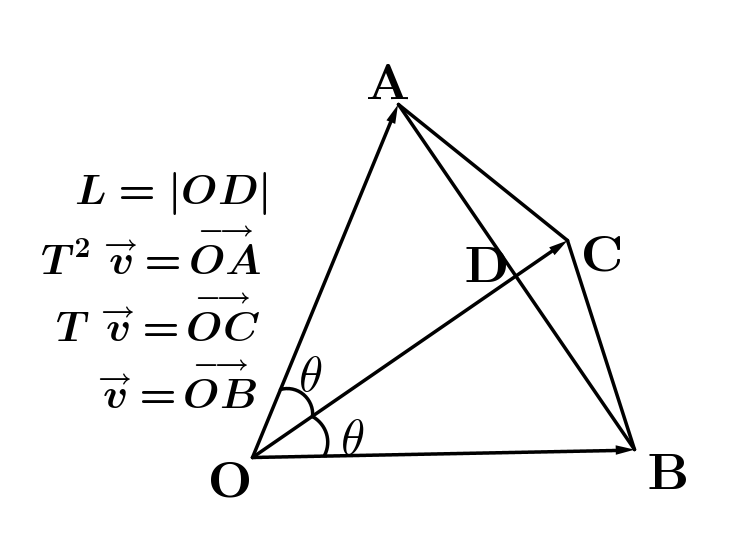
\includegraphics[scale=0.25]{./diagram.png} $\left\{\begin{array}{l}Tv=\displaystyle\frac{|\overset{\rightarrow}{v}|}{2L}(T^2 v+v)\Rightarrow T=\frac{|\overset{\rightarrow}{v}|}{2L}(T^2+I)\\\\ \displaystyle L=|\overset{\rightarrow}{v}|\cos\theta\Rightarrow\frac{|\overset{\rightarrow}{v}|}{2L}=\frac{1}{2\cos\theta}\end{array}\right.$\par{\tiny\,\par}\quad
Hence $p(T)=T^2-2\cos\theta T+I=0.$ $z^2-2\cos\theta z+1$ is the mini poly of $T.\quad\square$\par
{\tiny \_\,\_\,\_\,\_\,\_\,\_\,\_\,\_\,\_\,\_\,\_\,\_\,\_\,\_\,\_\,\_\,\_\,\_\,\_\,\_\,\_\,\_\,\_\,\_\,\_\,\_\,\_\,\_\,\_\,\_\,\_\,\_\,\_\,\_\,\_\,\_\,\_\,\_\,\_\,\_\,\_\,\_\,\_\,\_\,\_\,\_\,\_\,\_\,\_\,\_\,\_\,\_\,\_\,\_\,\_\,\_\,\_\,\_\,\_\,\_\,\_\,\_\,\_\,\_\,\_\,\_\,\_\,\_\,\_\,\_\,\_\_\,\_\,\_\,\_\,\_\,\_\,\_\,\_\,\_\,\_\,\_\,\_\,\_\,\_\,\_\,\_\,\_\,\_\,\_\,\_\,\_\,\_\,\_\,\_\,\_\,\_\,\_\,\_\,\_\,\_\,\_\,\_\,\_\,\_\,\_\,\_\,\_\,\_\,\_\,\_\,\_\,\_\,\_\,\_\,\_\,\_\,\_\,\_\,\_\,\_\,\_\,\_\,\_\,\_\,\_\,\_\,\_\,\_\,\_\,\_\,\_\,\_\,\_\,\_\,\_\,\_\,\_\,\_\,\_\,\_\,\_}\par{\tiny\,\par}

{\small $\bullet$} ({\normalsize 4E 5.B.11})\par\,\, {\timessl\Large Suppose $V$ is a two-dim vecsp, $T\in\Lm(V)$, and the matrix of $T$}\par\,\,
{\timessl\Large with respect to some basis of \,$V$ is {\large$\begin{pmatrix} a & c\\ b & d\end{pmatrix}.$
}}\par\,\,
(a) {\timessl\Large Show that $T^2 - (a + d)T + (ad - bc)I = 0.$}\par\,\,
(b) {\timessl\Large Show that the mini poly of $T$ equals}\par{\tiny\,\par}\qquad
\centerline{\timessl$\left\{\begin{array}{l}$
$z-a\qquad\qquad\qquad\qquad\qquad$ if $b=c=0$ and $a=d$,$\\ $
$z^2-(a+d)z+(ad-bc)\quad$ \,\,otherwise.
$\end{array}\right.$}
\par
{\timesbf S\footnotesize{OLUTION:}}\par\quad
(a) Suppose the basis is $(v,w)$. Because $\left\{\begin{array}{l}\displaystyle Tv=av+bw\Rightarrow (T-aI)v=bw,$ then apply $(T-dI)$ to both sides. $\\ Tw=cv+dw\Rightarrow (T-dI)w=cv,$ then apply $(T-aI)$ to both sides. $\end{array}\right.$\par{\tiny\,\par}\qquad\,
Hence $(T-aI)(T-dI)=bc I\Rightarrow T^2 - (a + d)T + (ad - bc)I = 0.$\par\quad
(b) If $b=c=0$ and $a=d.$ Then $\Mt(T)=${\small$\begin{pmatrix}a & 0\\ 0 & a\end{pmatrix}$}$=a\Mt(I)$. Thus $T=aI.$ Hence the mini poly is $z-a.$\par\qquad\,
Otherwise, by (a), $z^2-(a+d)z+(ad-bc)$ is a polynomial multiple of the mini poly.\par\qquad\,
Now we prove that $T\not\in\Spn(I),$ so that then the mini poly of $T$ has exactly degree $2.$\par\qquad\,
$($ At least one of the assumption of (I),(II) below is true. $)$\par\qquad\,
(I) Suppose $a=d,$ then $Tv=av+bw\not\in\Spn(v),Tw=cv+aw\not\in\Spn(w).$\par\qquad
(II) Suppose at most one of $b,c$ is not $0.$ If $b=0,$ then $Tw\not\in\Spn(w);$ If $c=0,$ then $Tv\not\in\Spn(v).\quad\square$\par
{\tiny \_\,\_\,\_\,\_\,\_\,\_\,\_\,\_\,\_\,\_\,\_\,\_\,\_\,\_\,\_\,\_\,\_\,\_\,\_\,\_\,\_\,\_\,\_\,\_\,\_\,\_\,\_\,\_\,\_\,\_\,\_\,\_\,\_\,\_\,\_\,\_\,\_\,\_\,\_\,\_\,\_\,\_\,\_\,\_\,\_\,\_\,\_\,\_\,\_\,\_\,\_\,\_\,\_\,\_\,\_\,\_\,\_\,\_\,\_\,\_\,\_\,\_\,\_\,\_\,\_\,\_\,\_\,\_\,\_\,\_\,\_\_\,\_\,\_\,\_\,\_\,\_\,\_\,\_\,\_\,\_\,\_\,\_\,\_\,\_\,\_\,\_\,\_\,\_\,\_\,\_\,\_\,\_\,\_\,\_\,\_\,\_\,\_\,\_\,\_\,\_\,\_\,\_\,\_\,\_\,\_\,\_\,\_\,\_\,\_\,\_\,\_\,\_\,\_\,\_\,\_\,\_\,\_\,\_\,\_\,\_\,\_\,\_\,\_\,\_\,\_\,\_\,\_\,\_\,\_\,\_\,\_\,\_\,\_\,\_\,\_\,\_\,\_\,\_\,\_\,\_\,\_}\par

{\timesbf\Large 5} {\timessl\Large 
Suppose $S,T\in\Lm(V),S$ is invertible, and $p\in\Po(${\timesbf F}$)$. Prove that $p(TS) = S^{-1} p(ST)S.$
}\par
{\timesbf S\footnotesize{OLUTION:}}\,\,\,We prove $(TS)^m=S^{-1}(ST)^m S$ for each $m\in\Nbfc\,$ by induction.\par\quad
(i) $m=0,1.$ $TS^{0}=I=S^{-1}(ST)^{0}S;\,\,\,TS=S^{-1}(ST)S.$\par\,\,\,
(ii) $m>1.$ Assume that $(TS)^{m}=S^{-1}(ST)^{m} S.$\par\qquad\qquad\quad\,
Then $(TS)^{m+1}=(TS)^{m}(TS)=S^{-1}(ST)^{m} STS=S^{-1}(ST)^{m+1} S.$\par\quad
Hence $\forall p\in\Po(${\timesbf F}$),p(TS)=a_0 (TS)^0+a_1 (TS)+\dots+a_m (TS)^m$\par\qquad\qquad\qquad\qquad\qquad\quad\,
$=a_0 [S^{-1}(ST)^0 S] +a_1 [S^{-1}(ST)S]+\dots+a_m [S^{-1}(ST)^{m} S]$\par\qquad\qquad\qquad\qquad\qquad\quad\,
$=S^{-1}[a_0 (ST)^0+a_1 (ST)+\dots+a_m (ST)^m]S=S^{-1}p(ST)S.\quad\square$\par
{\tiny \_\,\_\,\_\,\_\,\_\,\_\,\_\,\_\,\_\,\_\,\_\,\_\,\_\,\_\,\_\,\_\,\_\,\_\,\_\,\_\,\_\,\_\,\_\,\_\,\_\,\_\,\_\,\_\,\_\,\_\,\_\,\_\,\_\,\_\,\_\,\_\,\_\,\_\,\_\,\_\,\_\,\_\,\_\,\_\,\_\,\_\,\_\,\_\,\_\,\_\,\_\,\_\,\_\,\_\,\_\,\_\,\_\,\_\,\_\,\_\,\_\,\_\,\_\,\_\,\_\,\_\,\_\,\_\,\_\,\_\,\_\_\,\_\,\_\,\_\,\_\,\_\,\_\,\_\,\_\,\_\,\_\,\_\,\_\,\_\,\_\,\_\,\_\,\_\,\_\,\_\,\_\,\_\,\_\,\_\,\_\,\_\,\_\,\_\,\_\,\_\,\_\,\_\,\_\,\_\,\_\,\_\,\_\,\_\,\_\,\_\,\_\,\_\,\_\,\_\,\_\,\_\,\_\,\_\,\_\,\_\,\_\,\_\,\_\,\_\,\_\,\_\,\_\,\_\,\_\,\_\,\_\,\_\,\_\,\_\,\_\,\_\,\_\,\_\,\_\,\_\,\_\par}

{\small $\bullet$} ({\normalsize 4E 5.B.7})\par\,\,
(a) {\timessl\Large Give an example of $S, T\in\Lm(${\timesbf F}$^2)$ such that}\par\qquad
{\timessl\Large the mini poly of
$ST$ does not equal the mini poly of $TS$.}\par\,\,
(b) {\timessl\Large Suppose $V$ is finite-dim and $S, T\in\Lm(V)$. Prove that if $S$ or $T$ is invertible,}\par\qquad
{\timessl\Large then the mini poly of $ST$ equals the mini poly of $TS$.
}\par
{\timesbf S\footnotesize{OLUTION:}}\par\quad
(a) %Let $V=\Fbfc^{\infty},$ $S\in\Lm(${\timesbf F}$^\infty)$ is the forward shift operator, $T\in\Lm(${\timesbf F}$^\infty)$ is the backward shift operator.\par\qquad\,
%Then $ST(x_1,x_2,x_3,\dots)=(0,x_2,x_3,\dots)\Rightarrow 0,1$ are all the eigvals of $ST,$ $(ST)^2-(ST)=0.$\par\qquad\,
%$TS(x_1,x_2,\dots)=(x_1,x_2,\dots)\Rightarrow 1$ is the only eigval of $TS,$ $TS=I.$\par\qquad\,
Define $S$ by $S(x,y)=(x,x).$ Define $T$ by $T(x,y)=(0,y).$\par\qquad\,
Then $ST(x,y)=0,\,\,TS(x,y)=(0,x)$ for all $(x,y)\in\Fbfc^2.$\par\qquad\,
Thus $ST=0\neq TS$ and $(TS)^2=0.$\par\qquad\,
Hence the mini poly of $ST$ does not equal to the mini poly of $TS.$\par\quad
(b) Denote the mini poly of $ST$ by $p,$ and the mini poly $TS$ by $q.$\par\qquad\,
Suppose $S$ is invertible.\par\quad\,\,
$\left.\begin{array}{l}$
$p(ST)=0=S p(TS)S^{-1}\Rightarrow p(TS)=0,p$ is a polynomial multiple of $q.\\ $
$q(TS)=0=S^{-1} q(ST)S\Rightarrow q(ST)=0,q$ is a polynomial multiple of $p.$
$\end{array}\right\}\Rightarrow p=q.$\par{\tiny\,\par}\qquad\,
Reversing the roles of $S$ and $T$, we conclude that if $T$ is invertible, then $p=q$ as well.\quad$\square$\par
{\tiny \_\,\_\,\_\,\_\,\_\,\_\,\_\,\_\,\_\,\_\,\_\,\_\,\_\,\_\,\_\,\_\,\_\,\_\,\_\,\_\,\_\,\_\,\_\,\_\,\_\,\_\,\_\,\_\,\_\,\_\,\_\,\_\,\_\,\_\,\_\,\_\,\_\,\_\,\_\,\_\,\_\,\_\,\_\,\_\,\_\,\_\,\_\,\_\,\_\,\_\,\_\,\_\,\_\,\_\,\_\,\_\,\_\,\_\,\_\,\_\,\_\,\_\,\_\,\_\,\_\,\_\,\_\,\_\,\_\,\_\,\_\_\,\_\,\_\,\_\,\_\,\_\,\_\,\_\,\_\,\_\,\_\,\_\,\_\,\_\,\_\,\_\,\_\,\_\,\_\,\_\,\_\,\_\,\_\,\_\,\_\,\_\,\_\,\_\,\_\,\_\,\_\,\_\,\_\,\_\,\_\,\_\,\_\,\_\,\_\,\_\,\_\,\_\,\_\,\_\,\_\,\_\,\_\,\_\,\_\,\_\,\_\,\_\,\_\,\_\,\_\,\_\,\_\,\_\,\_\,\_\,\_\,\_\,\_\,\_\,\_\,\_\,\_\,\_\,\_\,\_\,\_}\par

{\small $\bullet$} ({\normalsize 4E 5.B.9})\par\,\, {\timessl\Large 
Suppose $T\in\Lm(V)$ is such that with respect to some basis of \,$V$,}\par\,\,
{\timessl\Large all entries of the matrix of $T$ are rational numbers.}\par\,\,
{\timessl\Large Explain why all coefficients of the mini poly of $T$ are rational numbers.
}\par
{\timesbf S\footnotesize{OLUTION:}}\par\quad
Let $(v_1,\dots,v_n)$ denote the basis such that $\Mt(T,(v_1,\dots,v_n))_{j,k}=A_{j,k}\in$ {\timesbf Q} for all $j,k=1,\dots,n$.\par\quad
Denote $\Mt(v_j,(v_1,\dots,v_n))$ by $x_j$ for each $v_j.$\par\quad
Suppose $p$ is the mini poly of $T$ and $p(z)=z^m+\dots+c_1 z+c_0.$ Now we show that each $c_j\in$ {\timesbf Q}.\par\quad
Note that $\forall s\in\Nbp,\Mt(T^s)=\Mt(T)^s=A^s\in$ {\timesbf Q}$^{n,n}$ and $T^s v_k=A^s_{1,k} v_1+\dots+A^s_{n,k}v_n$ for all $k\in\{1,\dots,n\}.$\par{\tiny\,\par}\quad
Thus $\left\{\begin{array}{l}
\Mt(p(T)v_1)=(A^m+\dots+c_1 A+c_0 I)x_1=\sum\limits_{j=1}^n(A^m+\dots+c_1 A+c_0 I)_{j,1}x_j=0;\\ \qquad\qquad\vdots \\
\Mt(p(T)v_n)=(A^m+\dots+c_1 A+c_0 I)x_n=\sum\limits_{j=1}^n(A^m+\dots+c_1 A+c_0 I)_{j,n}x_j=0;
\end{array}\right.$\par\quad
More clearly, $\left\{\begin{array}{l}
(A^m+\dots+c_1 A+c_0 I)_{1,1}=\cdots=(A^m+\dots+c_1 A+c_0 I)_{n,1}=0;\\ \qquad\qquad\qquad\qquad\qquad\,\,\,\vdots\quad\,\ddots\qquad\qquad\qquad\qquad\qquad\quad\,\,\,\,\,\vdots \\
(A^m+\dots+c_1 A+c_0 I)_{1,n}=\cdots=(A^m+\dots+c_1 A+c_0 I)_{n,n}=0;
\end{array}\right.$\par\quad
Hence we get a system of $n^2$ linear equations in $m$ unknowns $c_0,c_1,\dots,c_{m-1}.$\par\quad
We conclude that $c_0,c_1,\dots,c_{m-1}\in$ {\timesbf Q}.\quad$\square$\par
{\tiny \_\,\_\,\_\,\_\,\_\,\_\,\_\,\_\,\_\,\_\,\_\,\_\,\_\,\_\,\_\,\_\,\_\,\_\,\_\,\_\,\_\,\_\,\_\,\_\,\_\,\_\,\_\,\_\,\_\,\_\,\_\,\_\,\_\,\_\,\_\,\_\,\_\,\_\,\_\,\_\,\_\,\_\,\_\,\_\,\_\,\_\,\_\,\_\,\_\,\_\,\_\,\_\,\_\,\_\,\_\,\_\,\_\,\_\,\_\,\_\,\_\,\_\,\_\,\_\,\_\,\_\,\_\,\_\,\_\,\_\,\_\_\,\_\,\_\,\_\,\_\,\_\,\_\,\_\,\_\,\_\,\_\,\_\,\_\,\_\,\_\,\_\,\_\,\_\,\_\,\_\,\_\,\_\,\_\,\_\,\_\,\_\,\_\,\_\,\_\,\_\,\_\,\_\,\_\,\_\,\_\,\_\,\_\,\_\,\_\,\_\,\_\,\_\,\_\,\_\,\_\,\_\,\_\,\_\,\_\,\_\,\_\,\_\,\_\,\_\,\_\,\_\,\_\,\_\,\_\,\_\,\_\,\_\,\_\,\_\,\_\,\_\,\_\,\_\,\_\,\_\,\_}\par

{\timesbf\Large 11} {\timessl\Large 
Suppose $\Fbf = \Cbfc,$ $T\in\Lm(V), p\in\Po(${\timesbf C}$)$, and $\alpha\in\Cbfc.$
}\par\quad\,
{\timessl\Large Prove that $\alpha$ is an eigval of $p(T)$ $\Longleftrightarrow$ $\alpha = p(\lambda)$ for some eigval $\lambda$ of $T$.
}\par
{\timesbf S\footnotesize{OLUTION:}}\par\quad
(a) Suppose $\alpha$ is an eigval of $p(T)\Rightarrow (p(T)-\alpha I)$ is not injective.\par\qquad\,
Write $p(z)-\alpha=c(z-\lambda_1)\cdots(z-\lambda_m)\Rightarrow p(T)-\alpha I=c(T-\lambda_1 I)\cdots(T-\lambda_m I).$\par\qquad\,
By T{\small IPS,} $\,\exists\,(T-\lambda_j I)$ not injective. Thus $p(\lambda_j)-\alpha=0.\quad\square$\par\quad
(b) Suppose $\alpha=p(\lambda)$ and $\lambda$ is an eigval of $T$.\par\qquad\,
Define $q$ by $q(z)=p(z)-\alpha=c(z-\lambda_1)\cdots(z-\lambda_m).$ Then $\lambda$ is a zero of $q.$\par\qquad\,
Thus $q(T)=p(T)-\alpha I$ is not injective.
\par
{\tiny \_\,\_\,\_\,\_\,\_\,\_\,\_\,\_\,\_\,\_\,\_\,\_\,\_\,\_\,\_\,\_\,\_\,\_\,\_\,\_\,\_\,\_\,\_\,\_\,\_\,\_\,\_\,\_\,\_\,\_\,\_\,\_\,\_\,\_\,\_\,\_\,\_\,\_\,\_\,\_\,\_\,\_\,\_\,\_\,\_\,\_\,\_\,\_\,\_\,\_\,\_\,\_\,\_\,\_\,\_\,\_\,\_\,\_\,\_\,\_\,\_\,\_\,\_\,\_\,\_\,\_\,\_\,\_\,\_\,\_\,\_\_\,\_\,\_\,\_\,\_\,\_\,\_\,\_\,\_\,\_\,\_\,\_\,\_\,\_\,\_\,\_\,\_\,\_\,\_\,\_\,\_\,\_\,\_\,\_\,\_\,\_\,\_\,\_\,\_\,\_\,\_\,\_\,\_\,\_\,\_\,\_\,\_\,\_\,\_\,\_\,\_\,\_\,\_\,\_\,\_\,\_\,\_\,\_\,\_\,\_\,\_\,\_\,\_\,\_\,\_\,\_\,\_\,\_\,\_\,\_\,\_\,\_\,\_\,\_\,\_\,\_\,\_\,\_\,\_\,\_\,\_}\par

{\timesbf\Large 12} {\timessl\Large 
Give an example of an operator on $\Rbfc^2$
}\par\quad\,
{\timessl\Large that shows the result above does not hold if {\timesbf C} is replaced with {\timesbf R}.
}\par
{\timesbf S\footnotesize{OLUTION:}}\par\quad

\par
{\tiny \_\,\_\,\_\,\_\,\_\,\_\,\_\,\_\,\_\,\_\,\_\,\_\,\_\,\_\,\_\,\_\,\_\,\_\,\_\,\_\,\_\,\_\,\_\,\_\,\_\,\_\,\_\,\_\,\_\,\_\,\_\,\_\,\_\,\_\,\_\,\_\,\_\,\_\,\_\,\_\,\_\,\_\,\_\,\_\,\_\,\_\,\_\,\_\,\_\,\_\,\_\,\_\,\_\,\_\,\_\,\_\,\_\,\_\,\_\,\_\,\_\,\_\,\_\,\_\,\_\,\_\,\_\,\_\,\_\,\_\,\_\_\,\_\,\_\,\_\,\_\,\_\,\_\,\_\,\_\,\_\,\_\,\_\,\_\,\_\,\_\,\_\,\_\,\_\,\_\,\_\,\_\,\_\,\_\,\_\,\_\,\_\,\_\,\_\,\_\,\_\,\_\,\_\,\_\,\_\,\_\,\_\,\_\,\_\,\_\,\_\,\_\,\_\,\_\,\_\,\_\,\_\,\_\,\_\,\_\,\_\,\_\,\_\,\_\,\_\,\_\,\_\,\_\,\_\,\_\,\_\,\_\,\_\,\_\,\_\,\_\,\_\,\_\,\_\,\_\,\_\,\_}\par

{\small $\bullet$} ({\normalsize4E 5.B.17})\par\,\, {\timessl\Large 
Suppose $V$ is finite-dim, $T\in \Lm(V)$, and $p$ is the mini poly of $T$. Suppose $\lambda \in\Fbfc.$}\par\,\,
{\timessl\Large Show that the mini poly of $(T - \lambda I)$ is the polynomial $q$ defined by $q(z) = p(z + \lambda).$
}\par
{\timesbf S\footnotesize{OLUTION:}}\par\quad

\par
{\tiny \_\,\_\,\_\,\_\,\_\,\_\,\_\,\_\,\_\,\_\,\_\,\_\,\_\,\_\,\_\,\_\,\_\,\_\,\_\,\_\,\_\,\_\,\_\,\_\,\_\,\_\,\_\,\_\,\_\,\_\,\_\,\_\,\_\,\_\,\_\,\_\,\_\,\_\,\_\,\_\,\_\,\_\,\_\,\_\,\_\,\_\,\_\,\_\,\_\,\_\,\_\,\_\,\_\,\_\,\_\,\_\,\_\,\_\,\_\,\_\,\_\,\_\,\_\,\_\,\_\,\_\,\_\,\_\,\_\,\_\,\_\_\,\_\,\_\,\_\,\_\,\_\,\_\,\_\,\_\,\_\,\_\,\_\,\_\,\_\,\_\,\_\,\_\,\_\,\_\,\_\,\_\,\_\,\_\,\_\,\_\,\_\,\_\,\_\,\_\,\_\,\_\,\_\,\_\,\_\,\_\,\_\,\_\,\_\,\_\,\_\,\_\,\_\,\_\,\_\,\_\,\_\,\_\,\_\,\_\,\_\,\_\,\_\,\_\,\_\,\_\,\_\,\_\,\_\,\_\,\_\,\_\,\_\,\_\,\_\,\_\,\_\,\_\,\_\,\_\,\_\,\_}\par

{\small $\bullet$} ({\normalsize4E 5.B.18})\par\,\, {\timessl\Large 
Suppose $V$ is finite-dim, $T\in \Lm(V)$, and $p$ is the mini poly of $T$. Suppose $\lambda \in\Fbfc\backslash\{0\}$.}\par\,\,
{\timessl\Large Show that the mini poly of $\lambda T$ is the polynomial q defined by $q(z) = \lambda^{\deg p} p(\frac{z}{\lambda})$.
}\par
{\timesbf S\footnotesize{OLUTION:}}\par\quad

\par
{\tiny \_\,\_\,\_\,\_\,\_\,\_\,\_\,\_\,\_\,\_\,\_\,\_\,\_\,\_\,\_\,\_\,\_\,\_\,\_\,\_\,\_\,\_\,\_\,\_\,\_\,\_\,\_\,\_\,\_\,\_\,\_\,\_\,\_\,\_\,\_\,\_\,\_\,\_\,\_\,\_\,\_\,\_\,\_\,\_\,\_\,\_\,\_\,\_\,\_\,\_\,\_\,\_\,\_\,\_\,\_\,\_\,\_\,\_\,\_\,\_\,\_\,\_\,\_\,\_\,\_\,\_\,\_\,\_\,\_\,\_\,\_\_\,\_\,\_\,\_\,\_\,\_\,\_\,\_\,\_\,\_\,\_\,\_\,\_\,\_\,\_\,\_\,\_\,\_\,\_\,\_\,\_\,\_\,\_\,\_\,\_\,\_\,\_\,\_\,\_\,\_\,\_\,\_\,\_\,\_\,\_\,\_\,\_\,\_\,\_\,\_\,\_\,\_\,\_\,\_\,\_\,\_\,\_\,\_\,\_\,\_\,\_\,\_\,\_\,\_\,\_\,\_\,\_\,\_\,\_\,\_\,\_\,\_\,\_\,\_\,\_\,\_\,\_\,\_\,\_\,\_\,\_}\par

{\timesbf\Large 18} ({\normalsize O{\small R} 4E 5.B.15})\par\quad\, {\timessl\Large 
Suppose $V$ is a finite-dim complex vector space with $\dim V > 0$ and $T\in\Lm(V)$.}\par\quad\,
{\timessl\Large Define $f:\Cbf\rightarrow\Rbf\,$by $f(\lambda) = \dim \range(T-\lambda I)$.
Prove that $f$ is not a continuous function.
}\par
{\timesbf S\footnotesize{OLUTION:}}\par\quad

\par
{\tiny \_\,\_\,\_\,\_\,\_\,\_\,\_\,\_\,\_\,\_\,\_\,\_\,\_\,\_\,\_\,\_\,\_\,\_\,\_\,\_\,\_\,\_\,\_\,\_\,\_\,\_\,\_\,\_\,\_\,\_\,\_\,\_\,\_\,\_\,\_\,\_\,\_\,\_\,\_\,\_\,\_\,\_\,\_\,\_\,\_\,\_\,\_\,\_\,\_\,\_\,\_\,\_\,\_\,\_\,\_\,\_\,\_\,\_\,\_\,\_\,\_\,\_\,\_\,\_\,\_\,\_\,\_\,\_\,\_\,\_\,\_\_\,\_\,\_\,\_\,\_\,\_\,\_\,\_\,\_\,\_\,\_\,\_\,\_\,\_\,\_\,\_\,\_\,\_\,\_\,\_\,\_\,\_\,\_\,\_\,\_\,\_\,\_\,\_\,\_\,\_\,\_\,\_\,\_\,\_\,\_\,\_\,\_\,\_\,\_\,\_\,\_\,\_\,\_\,\_\,\_\,\_\,\_\,\_\,\_\,\_\,\_\,\_\,\_\,\_\,\_\,\_\,\_\,\_\,\_\,\_\,\_\,\_\,\_\,\_\,\_\,\_\,\_\,\_\,\_\,\_\,\_}\par

{\small $\bullet$} {\normalsize O{\small R} (4E 5.B.16), O{\small R} (8.C.18})\par\,\, {\timessl\Large 
Suppose $a_0 ,\dots, a_{n-1}\in\Fbfc.$ Let $T$ be the operator on $\Fbfc^n$ such that}\par{\tiny\,\par}\,\,
{\timessl\Large $\Mt(T)=\,${\normalsize$\begin{pmatrix}
0 &     &       &       &   &   -a_0\\
1 &  0  &       &       &   &   -a_1\\
  &  1  & \ddots&       &   & \vdots\\
  &     & \ddots&       & 0 &   -a_{n-2}\\
0 &     &       &       & 1 &   -a_{n-1}
\end{pmatrix} $}, with respect to the standard basis.
}\par{\tiny\,\par}\,\,
{\timessl\Large Show that the mini poly of $T$ is $a_0 + a_1 z + \dots + a_{n-1} z^{n-1} + z^n$.
}\par\,\,
{\timessl\small
$\Mt(T)$ is called the {\timessc companion matrix} of the poly above. This exercise shows that every monic poly is the mini poly of some operator.}{\par}\,\,
{\timessl\small Hence a formula or an algorithm that could produce exact eigvals for each operator on each $\Fbfc^n$ could then produce exact zeros for}{\footnotesize\par}\,\,
{\timessl\small each poly  $[$ by 8.36(b) $]$. Thus there is no such formula or algorithm. However, efficient numeric methods exist for obtaining very good}{\footnotesize\par}\,\,
{\timessl\small approximations for the eigvals of an operator.}{\footnotesize\par}
{\timesbf S\footnotesize{OLUTION:}}\par\quad

\par
{\tiny \_\,\_\,\_\,\_\,\_\,\_\,\_\,\_\,\_\,\_\,\_\,\_\,\_\,\_\,\_\,\_\,\_\,\_\,\_\,\_\,\_\,\_\,\_\,\_\,\_\,\_\,\_\,\_\,\_\,\_\,\_\,\_\,\_\,\_\,\_\,\_\,\_\,\_\,\_\,\_\,\_\,\_\,\_\,\_\,\_\,\_\,\_\,\_\,\_\,\_\,\_\,\_\,\_\,\_\,\_\,\_\,\_\,\_\,\_\,\_\,\_\,\_\,\_\,\_\,\_\,\_\,\_\,\_\,\_\,\_\,\_\_\,\_\,\_\,\_\,\_\,\_\,\_\,\_\,\_\,\_\,\_\,\_\,\_\,\_\,\_\,\_\,\_\,\_\,\_\,\_\,\_\,\_\,\_\,\_\,\_\,\_\,\_\,\_\,\_\,\_\,\_\,\_\,\_\,\_\,\_\,\_\,\_\,\_\,\_\,\_\,\_\,\_\,\_\,\_\,\_\,\_\,\_\,\_\,\_\,\_\,\_\,\_\,\_\,\_\,\_\,\_\,\_\,\_\,\_\,\_\,\_\,\_\,\_\,\_\,\_\,\_\,\_\,\_\,\_\,\_\,\_}\par

{\small $\bullet$} {\Large E{\normalsize IGENVALUES ON}  O{\normalsize DD}-D{\normalsize IMENSIONAL} R{\normalsize EAL} V{\normalsize ECTOR} S{\normalsize PACES}}\qquad (Eigvals on Odd-dim Real Vecsps)\par
{\small $\bullet$} {E{\small VEN}-D{\small IMENSIONAL} N{\small ULL} S{\small PACE}}\par\,\,
{\timessl\Large Suppose $\Fbf=\Rbfc,$ $V$ is finite-dim, $T\in\Lm(V)$ and $b, c\in\Rbf\,$with $b^2 < 4c$.}\par\,\,
{\timessl\Large Prove that $\dim\null(T^2 + bT + cI)$ is an even number.}\par
{\timesbf S\footnotesize{OLUTION:}}\par\quad
Denote $\null(T^2 + bT + cI)$ by $R.$ Then $T|_R+bT|_R+cI_R=(T+bT+cI)|_R=0\in\Lm(R).$\par\quad
Suppose $\lambda$ is an eigval of $T_R$ with an eigvec $v\in R.$\par\quad
Then $\displaystyle 0=(T|_R^2+bT|_R+cI_R)(v)=(\lambda^2+\lambda b+c)v=\left((\lambda+b)^2+c-\frac{b^2}{4}\right)v.$\par\quad
Because $\displaystyle c-\frac{b^2}{4}>0$ and we have $v=0.$ Thus $T_R$ has no eigvals.\par\quad
Let $U$ be an invariant subspace of $R$ that has the largest, even dim among all invariant subspaces.\par\quad
Assume that $U\neq R.$ Then $\,\exists\,w\in R$ but $w\not\in U.$ Let $W$ be such that $(w,T|_R w)$ is a basis of $W.$\par\quad
Because $T|_R^2 w=-bT|_R w-cw\in W.$ Hence $W$ is an invariant subspace of dim $2.$\par\quad
Thus $\dim (U+W)=\dim U+2-\dim(U\cap W),$ where $U\cap W=\{0\},$\par\qquad\qquad
for if not, because $w\not\in U,T|_R w\in U,$\par\qquad\qquad $U\cap W$ is invariant under $T|_R$ of one dim ( impossible because $T|_R$ has no eigvecs ).\par\quad
Hence $U+W$ is even-dim invariant subspace under $T|_R$, contradicting the maximality of $\dim U.$\par\quad
Thus the assumption was incorrect. Hence $R=\null(T^2+bT+cI)=U$ has even dim.\quad$\square$\par
{\tiny \_\,\_\,\_\,\_\,\_\,\_\,\_\,\_\,\_\,\_\,\_\,\_\,\_\,\_\,\_\,\_\,\_\,\_\,\_\,\_\,\_\,\_\,\_\,\_\,\_\,\_\,\_\,\_\,\_\,\_\,\_\,\_\,\_\,\_\,\_\,\_\,\_\,\_\,\_\,\_\,\_\,\_\,\_\,\_\,\_\,\_\,\_\,\_\,\_\,\_\,\_\,\_\,\_\,\_\,\_\,\_\,\_\,\_\,\_\,\_\,\_\,\_\,\_\,\_\,\_\,\_\,\_\,\_\,\_\,\_\,\_\_\,\_\,\_\,\_\,\_\,\_\,\_\,\_\,\_\,\_\,\_\,\_\,\_\,\_\,\_\,\_\,\_\,\_\,\_\,\_\,\_\,\_\,\_\,\_\,\_\,\_\,\_\,\_\,\_\,\_\,\_\,\_\,\_\,\_\,\_\,\_\,\_\,\_\,\_\,\_\,\_\,\_\,\_\,\_\,\_\,\_\,\_\,\_\,\_\,\_\,\_\,\_\,\_\,\_\,\_\,\_\,\_\,\_\,\_\,\_\,\_\,\_\,\_\,\_\,\_\,\_\,\_\,\_\,\_\,\_\,\_}{\tiny\,\par}
{\small $\bullet$} {O{\small PERATORS} O{\small N} O{\small DD}-D{\small IMENSIONAL} V{\small ECTOR} S{\small PACES} H{\small AVE} E{\small IGENVALUES}}\par\,\,
(a) Suppose $\Fbf=\Cbfc.$ Then by [5.21], we are done.\par\,\,
(b) {\timessl\Large Suppose $\Fbf=\Rbfc,$ $V$ is finite-dim, and $\dim V=n\neq 0$ is an odd number.\par\qquad
Let $T\in\Lm(V)$ and the mini poly is $p$. Prove that $T$ has an eigval.}\par
{\timesbf S\footnotesize{OLUTION:}}\par\quad
(i) If $n=1,$ then we are done.\par\,\,\,
(ii) $\,$Suppose $n\geq 3.$ Assume that every operator, on odd-dim vecsps of dim less than $n,$ has an eigval.\par\qquad\,
If $p$ is a polynomial multiple of $(x - \lambda)$ for some $\lambda\in\Rbfc,$ then by [8.49] $\lambda$ is an eigval of $T$ and we are done.\par\qquad\,
Now suppose $b, c\in\Rbf\,$such that $b^2 < 4c$ and $p$ is a polynomial multiple of $x^2 + bx + c$ (see [4.17]).\par\qquad\,
Then $\,\exists\,q\in\Po(${\timesbf R}$)$ such that $p(x) = q(x)(x^2 + bx + c)$ for all $x\in\Rbfc.$\par\qquad\,
Now $0 = p(T) = (q(T))(T^2 + bT + cI),$ which means that $q(T)|_{\range(T^2+bT+cI)}=0.$\par\qquad\,
Because $\deg q < \deg p$ and $p$ is the mini poly of $T$, hence $\range(T^2 + bT + cI)\neq V$.\par\qquad\,
又 $\dim V$ is odd and $\dim\null(T^2 +bT+cI)$ is even ( by our previous result ).\par\qquad\,
Thus $\dim V - \dim \null(T^2 + bT + cI)=\dim \range(T^2 + bT + cI)$ is odd.\par\qquad\,
By [5.18], $\range(T^2 + bT + cI)$ is an invariant subspace of $V$ under $T$ that has odd dim less than $n.$\par\qquad\,
Our induction hypothesis now implies that $T|_{\range(T^2 + bT + cI)}$ has an eigenvalue.\par\quad
By mathematical induction.\quad$\square$\par
{\tiny \_\,\_\,\_\,\_\,\_\,\_\,\_\,\_\,\_\,\_\,\_\,\_\,\_\,\_\,\_\,\_\,\_\,\_\,\_\,\_\,\_\,\_\,\_\,\_\,\_\,\_\,\_\,\_\,\_\,\_\,\_\,\_\,\_\,\_\,\_\,\_\,\_\,\_\,\_\,\_\,\_\,\_\,\_\,\_\,\_\,\_\,\_\,\_\,\_\,\_\,\_\,\_\,\_\,\_\,\_\,\_\,\_\,\_\,\_\,\_\,\_\,\_\,\_\,\_\,\_\,\_\,\_\,\_\,\_\,\_\,\_\_\,\_\,\_\,\_\,\_\,\_\,\_\,\_\,\_\,\_\,\_\,\_\,\_\,\_\,\_\,\_\,\_\,\_\,\_\,\_\,\_\,\_\,\_\,\_\,\_\,\_\,\_\,\_\,\_\,\_\,\_\,\_\,\_\,\_\,\_\,\_\,\_\,\_\,\_\,\_\,\_\,\_\,\_\,\_\,\_\,\_\,\_\,\_\,\_\,\_\,\_\,\_\,\_\,\_\,\_\,\_\,\_\,\_\,\_\,\_\,\_\,\_\,\_\,\_\,\_\,\_\,\_\,\_\,\_\,\_\,\_}\par

{\small $\bullet$} {\timessl\Large 
Suppose $\Fbf=\Rbfc,T\in\Lm(V)$ has no eigvals.}\par\quad\,
{\timessl\Large Prove that every invariant subspace of \,$V$ under $T$ is even-dim.
}\par
{\timesbf S\footnotesize{OLUTION:}}\par\quad
Suppose $U$ is such a subspace. Then $T|_U\in\Lm(U).$
We prove by contradiction.\par\quad
If $\dim U$ is odd, then $T|_U$ has an eigval and so is $T,$ so that $\,\exists$ invariant subspace of $1$ dim, contradicts.\quad$\square$\par
{\tiny \_\,\_\,\_\,\_\,\_\,\_\,\_\,\_\,\_\,\_\,\_\,\_\,\_\,\_\,\_\,\_\,\_\,\_\,\_\,\_\,\_\,\_\,\_\,\_\,\_\,\_\,\_\,\_\,\_\,\_\,\_\,\_\,\_\,\_\,\_\,\_\,\_\,\_\,\_\,\_\,\_\,\_\,\_\,\_\,\_\,\_\,\_\,\_\,\_\,\_\,\_\,\_\,\_\,\_\,\_\,\_\,\_\,\_\,\_\,\_\,\_\,\_\,\_\,\_\,\_\,\_\,\_\,\_\,\_\,\_\,\_\_\,\_\,\_\,\_\,\_\,\_\,\_\,\_\,\_\,\_\,\_\,\_\,\_\,\_\,\_\,\_\,\_\,\_\,\_\,\_\,\_\,\_\,\_\,\_\,\_\,\_\,\_\,\_\,\_\,\_\,\_\,\_\,\_\,\_\,\_\,\_\,\_\,\_\,\_\,\_\,\_\,\_\,\_\,\_\,\_\,\_\,\_\,\_\,\_\,\_\,\_\,\_\,\_\,\_\,\_\,\_\,\_\,\_\,\_\,\_\,\_\,\_\,\_\,\_\,\_\,\_\,\_\,\_\,\_\,\_\,\_}\par

{\small $\bullet$} ({\normalsize4E 5.B.29})\par\,\, {\timessl\Large 
Show that every operator on a finite-dim vecsp of dim $\geq 2$}\par\,\,
{\timessl\Large has an invariant subspace of dim $2$.
}\par\,\,
{\timessl\small
Exercise $($4E 5.C.6$)$ will give an improvement of this result when $\Fbf=\Cbf.$
}\par
{\timesbf S\footnotesize{OLUTION:}}\par\quad
For any such vecsp $V$ and $T\in\Lm(V),$ then $\,\exists\,$ invariant $U_0$ of even-dim.\par\quad
Again for $T|_{U_0}\in\Lm(U_0),$ if $\dim U_0> 2,$ then $\,\exists\,$ invariant $U_1$ of even-dim;\par\qquad\qquad\qquad\qquad\qquad\quad\, otherwise, $\dim U_0=2$ and we are done.\par\quad
Thus after some steps, we get an invariant subspace $U$ of $V$ and $\dim U=2.\quad\square$\par
{\tiny \_\,\_\,\_\,\_\,\_\,\_\,\_\,\_\,\_\,\_\,\_\,\_\,\_\,\_\,\_\,\_\,\_\,\_\,\_\,\_\,\_\,\_\,\_\,\_\,\_\,\_\,\_\,\_\,\_\,\_\,\_\,\_\,\_\,\_\,\_\,\_\,\_\,\_\,\_\,\_\,\_\,\_\,\_\,\_\,\_\,\_\,\_\,\_\,\_\,\_\,\_\,\_\,\_\,\_\,\_\,\_\,\_\,\_\,\_\,\_\,\_\,\_\,\_\,\_\,\_\,\_\,\_\,\_\,\_\,\_\,\_\_\,\_\,\_\,\_\,\_\,\_\,\_\,\_\,\_\,\_\,\_\,\_\,\_\,\_\,\_\,\_\,\_\,\_\,\_\,\_\,\_\,\_\,\_\,\_\,\_\,\_\,\_\,\_\,\_\,\_\,\_\,\_\,\_\,\_\,\_\,\_\,\_\,\_\,\_\,\_\,\_\,\_\,\_\,\_\,\_\,\_\,\_\,\_\,\_\,\_\,\_\,\_\,\_\,\_\,\_\,\_\,\_\,\_\,\_\,\_\,\_\,\_\,\_\,\_\,\_\,\_\,\_\,\_\,\_\,\_\,\_}\par

\rightline{\timesbf\Large{E{\normalsize NDED}}}\par{\tiny\,\par}

{\huge\timesbf 5.B: II}

{\small $\bullet$} ({\normalsize4E 5.C.1})\par\,\, {\timessl\Large 
Prove or give a counterexample:}\par\,\,
{\timessl\Large If $T\in \Lm(V)$ and $T^2$ has an upper-trig matrix with respect to some basis of \,$V$,}\par\,\,
{\timessl\Large then $T$ has an upper-trig matrix with respect to some basis of \,$V$.
}\par
{\timesbf S\footnotesize{OLUTION:}}\par\quad

\par
{\tiny \_\,\_\,\_\,\_\,\_\,\_\,\_\,\_\,\_\,\_\,\_\,\_\,\_\,\_\,\_\,\_\,\_\,\_\,\_\,\_\,\_\,\_\,\_\,\_\,\_\,\_\,\_\,\_\,\_\,\_\,\_\,\_\,\_\,\_\,\_\,\_\,\_\,\_\,\_\,\_\,\_\,\_\,\_\,\_\,\_\,\_\,\_\,\_\,\_\,\_\,\_\,\_\,\_\,\_\,\_\,\_\,\_\,\_\,\_\,\_\,\_\,\_\,\_\,\_\,\_\,\_\,\_\,\_\,\_\,\_\,\_\_\,\_\,\_\,\_\,\_\,\_\,\_\,\_\,\_\,\_\,\_\,\_\,\_\,\_\,\_\,\_\,\_\,\_\,\_\,\_\,\_\,\_\,\_\,\_\,\_\,\_\,\_\,\_\,\_\,\_\,\_\,\_\,\_\,\_\,\_\,\_\,\_\,\_\,\_\,\_\,\_\,\_\,\_\,\_\,\_\,\_\,\_\,\_\,\_\,\_\,\_\,\_\,\_\,\_\,\_\,\_\,\_\,\_\,\_\,\_\,\_\,\_\,\_\,\_\,\_\,\_\,\_\,\_\,\_\,\_\,\_}\par

{\small $\bullet$} ({\normalsize4E 5.C.2})\par\,\, {\timessl\Large 
Suppose $A$ and $B$ are upper-trig matrices of the same size,}\par\,\,
{\timessl\Large with $\alpha_1 , \dots , \alpha_n$ on the diagonal of $A$ and $\beta_1 , \dots , \beta_n$ on the diagonal of $B$.
}\par\,\,
(a) {\timessl\Large Show that $A + B$ is an upper-trig matrix with $\alpha_1 + \beta_1 , \dots , \alpha_n + \beta_n$ on the diagonal.
}\par\,\,
(b) {\timessl\Large Show that $AB$ is an upper-trig matrix with $\alpha_1 \beta_1 , \dots , \alpha_n \beta_n$ on the diagonal.
}\par
{\timesbf S\footnotesize{OLUTION:}}\par\quad

\par
{\tiny \_\,\_\,\_\,\_\,\_\,\_\,\_\,\_\,\_\,\_\,\_\,\_\,\_\,\_\,\_\,\_\,\_\,\_\,\_\,\_\,\_\,\_\,\_\,\_\,\_\,\_\,\_\,\_\,\_\,\_\,\_\,\_\,\_\,\_\,\_\,\_\,\_\,\_\,\_\,\_\,\_\,\_\,\_\,\_\,\_\,\_\,\_\,\_\,\_\,\_\,\_\,\_\,\_\,\_\,\_\,\_\,\_\,\_\,\_\,\_\,\_\,\_\,\_\,\_\,\_\,\_\,\_\,\_\,\_\,\_\,\_\_\,\_\,\_\,\_\,\_\,\_\,\_\,\_\,\_\,\_\,\_\,\_\,\_\,\_\,\_\,\_\,\_\,\_\,\_\,\_\,\_\,\_\,\_\,\_\,\_\,\_\,\_\,\_\,\_\,\_\,\_\,\_\,\_\,\_\,\_\,\_\,\_\,\_\,\_\,\_\,\_\,\_\,\_\,\_\,\_\,\_\,\_\,\_\,\_\,\_\,\_\,\_\,\_\,\_\,\_\,\_\,\_\,\_\,\_\,\_\,\_\,\_\,\_\,\_\,\_\,\_\,\_\,\_\,\_\,\_\,\_}\par

{\small $\bullet$} ({\normalsize4E 5.C.3})\par\,\, {\timessl\Large 
Suppose $T\in \Lm(V)$ is invertible and $(v_1 , \dots , v_n)$ is a basis of \,$V$ with respect}\par\,\,
{\timessl\Large to which the matrix of $T$ is upper trig, with $\lambda_1 , \dots , \lambda_n$ on the diagonal.}\par\,\,
{\timessl\Large
Show that the matrix of $T^{-1}$ is also upper trig with respect to the same basis,}\par\,\,
{\timessl\Large with
{\normalsize$\displaystyle\frac{1}{\lambda_1},\dots,\frac{1}{\lambda_n}$} on the diagonal.
}\par
{\timesbf S\footnotesize{OLUTION:}}\par\quad

\par
{\tiny \_\,\_\,\_\,\_\,\_\,\_\,\_\,\_\,\_\,\_\,\_\,\_\,\_\,\_\,\_\,\_\,\_\,\_\,\_\,\_\,\_\,\_\,\_\,\_\,\_\,\_\,\_\,\_\,\_\,\_\,\_\,\_\,\_\,\_\,\_\,\_\,\_\,\_\,\_\,\_\,\_\,\_\,\_\,\_\,\_\,\_\,\_\,\_\,\_\,\_\,\_\,\_\,\_\,\_\,\_\,\_\,\_\,\_\,\_\,\_\,\_\,\_\,\_\,\_\,\_\,\_\,\_\,\_\,\_\,\_\,\_\_\,\_\,\_\,\_\,\_\,\_\,\_\,\_\,\_\,\_\,\_\,\_\,\_\,\_\,\_\,\_\,\_\,\_\,\_\,\_\,\_\,\_\,\_\,\_\,\_\,\_\,\_\,\_\,\_\,\_\,\_\,\_\,\_\,\_\,\_\,\_\,\_\,\_\,\_\,\_\,\_\,\_\,\_\,\_\,\_\,\_\,\_\,\_\,\_\,\_\,\_\,\_\,\_\,\_\,\_\,\_\,\_\,\_\,\_\,\_\,\_\,\_\,\_\,\_\,\_\,\_\,\_\,\_\,\_\,\_\,\_}\par

{\timesbf\Large 9} ({\normalsize4E 5.C.7})\par\,\, {\timessl\Large 
Suppose $V$ is finite-dim, $T\in \Lm(V)$, and $v \in V$.
}\par\,\,\,
(a) {\timessl\Large
Prove that $\,\exists\,!$ monic poly $p_v$ of smallest degree such that $p_v (T)v = 0$.
}\par\,\,\,
(b) {\timessl\Large
Prove that the mini poly of $T$ is a polynomial multiple of $p_v$.
}\par
{\timesbf S\footnotesize{OLUTION:}}\par\quad

\par
{\tiny \_\,\_\,\_\,\_\,\_\,\_\,\_\,\_\,\_\,\_\,\_\,\_\,\_\,\_\,\_\,\_\,\_\,\_\,\_\,\_\,\_\,\_\,\_\,\_\,\_\,\_\,\_\,\_\,\_\,\_\,\_\,\_\,\_\,\_\,\_\,\_\,\_\,\_\,\_\,\_\,\_\,\_\,\_\,\_\,\_\,\_\,\_\,\_\,\_\,\_\,\_\,\_\,\_\,\_\,\_\,\_\,\_\,\_\,\_\,\_\,\_\,\_\,\_\,\_\,\_\,\_\,\_\,\_\,\_\,\_\,\_\_\,\_\,\_\,\_\,\_\,\_\,\_\,\_\,\_\,\_\,\_\,\_\,\_\,\_\,\_\,\_\,\_\,\_\,\_\,\_\,\_\,\_\,\_\,\_\,\_\,\_\,\_\,\_\,\_\,\_\,\_\,\_\,\_\,\_\,\_\,\_\,\_\,\_\,\_\,\_\,\_\,\_\,\_\,\_\,\_\,\_\,\_\,\_\,\_\,\_\,\_\,\_\,\_\,\_\,\_\,\_\,\_\,\_\,\_\,\_\,\_\,\_\,\_\,\_\,\_\,\_\,\_\,\_\,\_\,\_\,\_}\par


{\timesbf\Large 14} ({\normalsize O{\small R} 4E 5.C.4})\par\quad\, {\timessl\Large 
Give an operator $T$ such that with respect to some basis, $\Mt(T)_{k,k}=0$ for each $k$,}\par\quad\,
{\timessl\Large while $T$ is invertible.
}\par
{\timesbf S\footnotesize{OLUTION:}}\par\quad

\par
{\tiny \_\,\_\,\_\,\_\,\_\,\_\,\_\,\_\,\_\,\_\,\_\,\_\,\_\,\_\,\_\,\_\,\_\,\_\,\_\,\_\,\_\,\_\,\_\,\_\,\_\,\_\,\_\,\_\,\_\,\_\,\_\,\_\,\_\,\_\,\_\,\_\,\_\,\_\,\_\,\_\,\_\,\_\,\_\,\_\,\_\,\_\,\_\,\_\,\_\,\_\,\_\,\_\,\_\,\_\,\_\,\_\,\_\,\_\,\_\,\_\,\_\,\_\,\_\,\_\,\_\,\_\,\_\,\_\,\_\,\_\,\_\_\,\_\,\_\,\_\,\_\,\_\,\_\,\_\,\_\,\_\,\_\,\_\,\_\,\_\,\_\,\_\,\_\,\_\,\_\,\_\,\_\,\_\,\_\,\_\,\_\,\_\,\_\,\_\,\_\,\_\,\_\,\_\,\_\,\_\,\_\,\_\,\_\,\_\,\_\,\_\,\_\,\_\,\_\,\_\,\_\,\_\,\_\,\_\,\_\,\_\,\_\,\_\,\_\,\_\,\_\,\_\,\_\,\_\,\_\,\_\,\_\,\_\,\_\,\_\,\_\,\_\,\_\,\_\,\_\,\_\,\_}\par

{\timesbf\Large 15} ({\normalsize O{\small R} 4E 5.C.5})\par\quad\, {\timessl\Large 
Give an operator $T$ such that with respect to some basis, $\Mt(T)_{k,k}\neq 0$ for each $k$,}\par\quad\,
{\timessl\Large while $T$ is not invertible.
}\par
{\timesbf S\footnotesize{OLUTION:}}\par\quad

\par
{\tiny \_\,\_\,\_\,\_\,\_\,\_\,\_\,\_\,\_\,\_\,\_\,\_\,\_\,\_\,\_\,\_\,\_\,\_\,\_\,\_\,\_\,\_\,\_\,\_\,\_\,\_\,\_\,\_\,\_\,\_\,\_\,\_\,\_\,\_\,\_\,\_\,\_\,\_\,\_\,\_\,\_\,\_\,\_\,\_\,\_\,\_\,\_\,\_\,\_\,\_\,\_\,\_\,\_\,\_\,\_\,\_\,\_\,\_\,\_\,\_\,\_\,\_\,\_\,\_\,\_\,\_\,\_\,\_\,\_\,\_\,\_\_\,\_\,\_\,\_\,\_\,\_\,\_\,\_\,\_\,\_\,\_\,\_\,\_\,\_\,\_\,\_\,\_\,\_\,\_\,\_\,\_\,\_\,\_\,\_\,\_\,\_\,\_\,\_\,\_\,\_\,\_\,\_\,\_\,\_\,\_\,\_\,\_\,\_\,\_\,\_\,\_\,\_\,\_\,\_\,\_\,\_\,\_\,\_\,\_\,\_\,\_\,\_\,\_\,\_\,\_\,\_\,\_\,\_\,\_\,\_\,\_\,\_\,\_\,\_\,\_\,\_\,\_\,\_\,\_\,\_\,\_}\par

{\timesbf\Large 20} ({\normalsize O{\small R} 4E 5.C.6})\par\quad\, {\timessl\Large 
Suppose $\Fbf=\Cbfc,$ $V$ is finite-dim, and $T\in\Lm(V)$.
}\par\quad\,
{\timessl\Large Prove that if $k\in\{1,\dots,\dim V\},$ then \,$V$ has a $k$ dim subspace invariant under $T$.
}\par
{\timesbf S\footnotesize{OLUTION:}}\par\quad

\par
{\tiny \_\,\_\,\_\,\_\,\_\,\_\,\_\,\_\,\_\,\_\,\_\,\_\,\_\,\_\,\_\,\_\,\_\,\_\,\_\,\_\,\_\,\_\,\_\,\_\,\_\,\_\,\_\,\_\,\_\,\_\,\_\,\_\,\_\,\_\,\_\,\_\,\_\,\_\,\_\,\_\,\_\,\_\,\_\,\_\,\_\,\_\,\_\,\_\,\_\,\_\,\_\,\_\,\_\,\_\,\_\,\_\,\_\,\_\,\_\,\_\,\_\,\_\,\_\,\_\,\_\,\_\,\_\,\_\,\_\,\_\,\_\_\,\_\,\_\,\_\,\_\,\_\,\_\,\_\,\_\,\_\,\_\,\_\,\_\,\_\,\_\,\_\,\_\,\_\,\_\,\_\,\_\,\_\,\_\,\_\,\_\,\_\,\_\,\_\,\_\,\_\,\_\,\_\,\_\,\_\,\_\,\_\,\_\,\_\,\_\,\_\,\_\,\_\,\_\,\_\,\_\,\_\,\_\,\_\,\_\,\_\,\_\,\_\,\_\,\_\,\_\,\_\,\_\,\_\,\_\,\_\,\_\,\_\,\_\,\_\,\_\,\_\,\_\,\_\,\_\,\_\,\_}\par


{\small $\bullet$} ({\normalsize 4E 5.C.8})\par\,\, {\timessl\Large 
Suppose $V$ is finite-dim, $T\in \Lm(V)$, and $\,\exists\,v \in V\backslash\{0\}$ such that $T^2 v + 2Tv = -2v$.
}\par\,\,
(a) {\timessl\Large
Prove that if $\Fbf=\Rbfc,$ then $\nexists$ a basis of \,$V$ with respect to which $T$ has an upper-trig matrix.
}\par\,\,
(b) {\timessl\Large
Prove that if $\Fbf=\Cbf\,$and $A$ is an upper-trig matrix that equals the matrix of $T$}\par\quad\,\,\,
{\timessl\Large with respect to some basis of \,$V$, then $-1 + \i$ or $-1 - \i$
appears on the diagonal of $A$.
}\par
{\timesbf S\footnotesize{OLUTION:}}\par\quad

\par
{\tiny \_\,\_\,\_\,\_\,\_\,\_\,\_\,\_\,\_\,\_\,\_\,\_\,\_\,\_\,\_\,\_\,\_\,\_\,\_\,\_\,\_\,\_\,\_\,\_\,\_\,\_\,\_\,\_\,\_\,\_\,\_\,\_\,\_\,\_\,\_\,\_\,\_\,\_\,\_\,\_\,\_\,\_\,\_\,\_\,\_\,\_\,\_\,\_\,\_\,\_\,\_\,\_\,\_\,\_\,\_\,\_\,\_\,\_\,\_\,\_\,\_\,\_\,\_\,\_\,\_\,\_\,\_\,\_\,\_\,\_\,\_\_\,\_\,\_\,\_\,\_\,\_\,\_\,\_\,\_\,\_\,\_\,\_\,\_\,\_\,\_\,\_\,\_\,\_\,\_\,\_\,\_\,\_\,\_\,\_\,\_\,\_\,\_\,\_\,\_\,\_\,\_\,\_\,\_\,\_\,\_\,\_\,\_\,\_\,\_\,\_\,\_\,\_\,\_\,\_\,\_\,\_\,\_\,\_\,\_\,\_\,\_\,\_\,\_\,\_\,\_\,\_\,\_\,\_\,\_\,\_\,\_\,\_\,\_\,\_\,\_\,\_\,\_\,\_\,\_\,\_\,\_}\par

{\small $\bullet$} ({\normalsize 4E 5.C.9})\par\,\, {\timessl\Large 
Suppose $B\in\Fbfc^{n,n}$ with complex entries.}\par\,\,
{\timessl\Large Prove that $\,\exists$ invertible $A\in\Fbfc^{n,n}$ with complex entries}\par\,\,
{\timessl\Large such that $A^{-1} BA$ is an upper-trig matrix.
}\par
{\timesbf S\footnotesize{OLUTION:}}\par\quad

\par
{\tiny \_\,\_\,\_\,\_\,\_\,\_\,\_\,\_\,\_\,\_\,\_\,\_\,\_\,\_\,\_\,\_\,\_\,\_\,\_\,\_\,\_\,\_\,\_\,\_\,\_\,\_\,\_\,\_\,\_\,\_\,\_\,\_\,\_\,\_\,\_\,\_\,\_\,\_\,\_\,\_\,\_\,\_\,\_\,\_\,\_\,\_\,\_\,\_\,\_\,\_\,\_\,\_\,\_\,\_\,\_\,\_\,\_\,\_\,\_\,\_\,\_\,\_\,\_\,\_\,\_\,\_\,\_\,\_\,\_\,\_\,\_\_\,\_\,\_\,\_\,\_\,\_\,\_\,\_\,\_\,\_\,\_\,\_\,\_\,\_\,\_\,\_\,\_\,\_\,\_\,\_\,\_\,\_\,\_\,\_\,\_\,\_\,\_\,\_\,\_\,\_\,\_\,\_\,\_\,\_\,\_\,\_\,\_\,\_\,\_\,\_\,\_\,\_\,\_\,\_\,\_\,\_\,\_\,\_\,\_\,\_\,\_\,\_\,\_\,\_\,\_\,\_\,\_\,\_\,\_\,\_\,\_\,\_\,\_\,\_\,\_\,\_\,\_\,\_\,\_\,\_\,\_}\par

{\small $\bullet$} ({\normalsize 4E 5.C.10})\par\,\,
 {\timessl\Large 
Suppose $T\in \Lm(V)$ and $(v_1 , \dots , v_n)$ is a basis of \,$V$.}\par\,\,
{\timessl\Large Show that the following are equivalent.
}\par\,\,
(a) {\timessl\Large
The matrix of $T$ with respect to $(v_1 , \dots , v_n)$ is lower trig.
}\par\,\,
(b) {\timessl\Large
$\Spn(v_k , \dots , v_n )$ is invariant under $T$ for each $k = 1, \dots , n$.
}\par\,\,
(c) {\timessl\Large
$Tv_k \in \Spn(v_k , \dots , v_n )$ for each $k = 1, \dots , n$.
}\par\,\,
{\timessl\small
A square matrix is called lower trig if all entries above the diagonal are $0$.}\par
{\timesbf S\footnotesize{OLUTION:}}\par\quad

\par
{\tiny \_\,\_\,\_\,\_\,\_\,\_\,\_\,\_\,\_\,\_\,\_\,\_\,\_\,\_\,\_\,\_\,\_\,\_\,\_\,\_\,\_\,\_\,\_\,\_\,\_\,\_\,\_\,\_\,\_\,\_\,\_\,\_\,\_\,\_\,\_\,\_\,\_\,\_\,\_\,\_\,\_\,\_\,\_\,\_\,\_\,\_\,\_\,\_\,\_\,\_\,\_\,\_\,\_\,\_\,\_\,\_\,\_\,\_\,\_\,\_\,\_\,\_\,\_\,\_\,\_\,\_\,\_\,\_\,\_\,\_\,\_\_\,\_\,\_\,\_\,\_\,\_\,\_\,\_\,\_\,\_\,\_\,\_\,\_\,\_\,\_\,\_\,\_\,\_\,\_\,\_\,\_\,\_\,\_\,\_\,\_\,\_\,\_\,\_\,\_\,\_\,\_\,\_\,\_\,\_\,\_\,\_\,\_\,\_\,\_\,\_\,\_\,\_\,\_\,\_\,\_\,\_\,\_\,\_\,\_\,\_\,\_\,\_\,\_\,\_\,\_\,\_\,\_\,\_\,\_\,\_\,\_\,\_\,\_\,\_\,\_\,\_\,\_\,\_\,\_\,\_\,\_}\par

{\small $\bullet$} ({\normalsize 4E 5.C.11})\par\,\, {\timessl\Large 
Suppose $\Fbf=\Cbf\,$and $V$ is finite-dim.}\par\,\,
{\timessl\Large Prove that if $T\in \Lm(V)$, then $T$ has a lower-trig matrix with respect to some basis.
}\par
{\timesbf S\footnotesize{OLUTION:}}\par\quad

\par
{\tiny \_\,\_\,\_\,\_\,\_\,\_\,\_\,\_\,\_\,\_\,\_\,\_\,\_\,\_\,\_\,\_\,\_\,\_\,\_\,\_\,\_\,\_\,\_\,\_\,\_\,\_\,\_\,\_\,\_\,\_\,\_\,\_\,\_\,\_\,\_\,\_\,\_\,\_\,\_\,\_\,\_\,\_\,\_\,\_\,\_\,\_\,\_\,\_\,\_\,\_\,\_\,\_\,\_\,\_\,\_\,\_\,\_\,\_\,\_\,\_\,\_\,\_\,\_\,\_\,\_\,\_\,\_\,\_\,\_\,\_\,\_\_\,\_\,\_\,\_\,\_\,\_\,\_\,\_\,\_\,\_\,\_\,\_\,\_\,\_\,\_\,\_\,\_\,\_\,\_\,\_\,\_\,\_\,\_\,\_\,\_\,\_\,\_\,\_\,\_\,\_\,\_\,\_\,\_\,\_\,\_\,\_\,\_\,\_\,\_\,\_\,\_\,\_\,\_\,\_\,\_\,\_\,\_\,\_\,\_\,\_\,\_\,\_\,\_\,\_\,\_\,\_\,\_\,\_\,\_\,\_\,\_\,\_\,\_\,\_\,\_\,\_\,\_\,\_\,\_\,\_\,\_}\par

{\small $\bullet$} ({\normalsize 4E 5.C.12})\par\,\, {\timessl\Large 
Suppose $V$ is finite-dim, $T\in \Lm(V)$ has an upper-trig matrix with respect to some basis,}\par\,\,
{\timessl\Large and $U$ is a subspace of \,$V$ that is invariant under $T$.
}\par\,\,
(a) {\timessl\Large
Prove that $T|_U$ has an upper-trig matrix with respect to some basis of $U$.}\par\,\,
(b) {\timessl\Large
Prove that $T/U$ has an upper-trig matrix with respect to some basis of \,$V/U$.
}\par
{\timesbf S\footnotesize{OLUTION:}}\par\quad

\par
{\tiny \_\,\_\,\_\,\_\,\_\,\_\,\_\,\_\,\_\,\_\,\_\,\_\,\_\,\_\,\_\,\_\,\_\,\_\,\_\,\_\,\_\,\_\,\_\,\_\,\_\,\_\,\_\,\_\,\_\,\_\,\_\,\_\,\_\,\_\,\_\,\_\,\_\,\_\,\_\,\_\,\_\,\_\,\_\,\_\,\_\,\_\,\_\,\_\,\_\,\_\,\_\,\_\,\_\,\_\,\_\,\_\,\_\,\_\,\_\,\_\,\_\,\_\,\_\,\_\,\_\,\_\,\_\,\_\,\_\,\_\,\_\_\,\_\,\_\,\_\,\_\,\_\,\_\,\_\,\_\,\_\,\_\,\_\,\_\,\_\,\_\,\_\,\_\,\_\,\_\,\_\,\_\,\_\,\_\,\_\,\_\,\_\,\_\,\_\,\_\,\_\,\_\,\_\,\_\,\_\,\_\,\_\,\_\,\_\,\_\,\_\,\_\,\_\,\_\,\_\,\_\,\_\,\_\,\_\,\_\,\_\,\_\,\_\,\_\,\_\,\_\,\_\,\_\,\_\,\_\,\_\,\_\,\_\,\_\,\_\,\_\,\_\,\_\,\_\,\_\,\_\,\_}\par

{\small $\bullet$} ({\normalsize 4E 5.C.13})\par\,\, {\timessl\Large 
Suppose $V$ is finite-dim and $T\in \Lm(V)$.}\par\,\,
{\timessl\Large Suppose $\,\exists\,U$ of \,$V$ that is invariant under $T$ such that}\par\,\,
{\timessl\Large $T|_U$ has an upper-trig matrix with respect to some basis of $U$}\par\,\,
{\timessl\Large and also $T/U$ has an upper-trig matrix with respect to some basis of \,$V/U$.}\par\,\,
{\timessl\Large Prove that $T$ has an upper-trig matrix with respect to some basis of \,$V$.
}\par
{\timesbf S\footnotesize{OLUTION:}}\par\quad

\par
{\tiny \_\,\_\,\_\,\_\,\_\,\_\,\_\,\_\,\_\,\_\,\_\,\_\,\_\,\_\,\_\,\_\,\_\,\_\,\_\,\_\,\_\,\_\,\_\,\_\,\_\,\_\,\_\,\_\,\_\,\_\,\_\,\_\,\_\,\_\,\_\,\_\,\_\,\_\,\_\,\_\,\_\,\_\,\_\,\_\,\_\,\_\,\_\,\_\,\_\,\_\,\_\,\_\,\_\,\_\,\_\,\_\,\_\,\_\,\_\,\_\,\_\,\_\,\_\,\_\,\_\,\_\,\_\,\_\,\_\,\_\,\_\_\,\_\,\_\,\_\,\_\,\_\,\_\,\_\,\_\,\_\,\_\,\_\,\_\,\_\,\_\,\_\,\_\,\_\,\_\,\_\,\_\,\_\,\_\,\_\,\_\,\_\,\_\,\_\,\_\,\_\,\_\,\_\,\_\,\_\,\_\,\_\,\_\,\_\,\_\,\_\,\_\,\_\,\_\,\_\,\_\,\_\,\_\,\_\,\_\,\_\,\_\,\_\,\_\,\_\,\_\,\_\,\_\,\_\,\_\,\_\,\_\,\_\,\_\,\_\,\_\,\_\,\_\,\_\,\_\,\_\,\_}\par

{\small $\bullet$} ({\normalsize 4E 5.C.14})\par\,\, {\timessl\Large 
Suppose $V$ is finite-dim and $T\in \Lm(V)$.}\par\,\,
{\timessl\Large Prove that $T$ has an upper-trig matrix with respect to some basis of \,$V$}\par\qquad\quad
{\timessl\Large $\Longleftrightarrow$ $T'$ has an upper-trig matrix with respect to some basis of \,$V'$.
}\par
{\timesbf S\footnotesize{OLUTION:}}\par\quad

\par
{\tiny \_\,\_\,\_\,\_\,\_\,\_\,\_\,\_\,\_\,\_\,\_\,\_\,\_\,\_\,\_\,\_\,\_\,\_\,\_\,\_\,\_\,\_\,\_\,\_\,\_\,\_\,\_\,\_\,\_\,\_\,\_\,\_\,\_\,\_\,\_\,\_\,\_\,\_\,\_\,\_\,\_\,\_\,\_\,\_\,\_\,\_\,\_\,\_\,\_\,\_\,\_\,\_\,\_\,\_\,\_\,\_\,\_\,\_\,\_\,\_\,\_\,\_\,\_\,\_\,\_\,\_\,\_\,\_\,\_\,\_\,\_\_\,\_\,\_\,\_\,\_\,\_\,\_\,\_\,\_\,\_\,\_\,\_\,\_\,\_\,\_\,\_\,\_\,\_\,\_\,\_\,\_\,\_\,\_\,\_\,\_\,\_\,\_\,\_\,\_\,\_\,\_\,\_\,\_\,\_\,\_\,\_\,\_\,\_\,\_\,\_\,\_\,\_\,\_\,\_\,\_\,\_\,\_\,\_\,\_\,\_\,\_\,\_\,\_\,\_\,\_\,\_\,\_\,\_\,\_\,\_\,\_\,\_\,\_\,\_\,\_\,\_\,\_\,\_\,\_\,\_\,\_}\par

\rightline{\timesbf\Large{E{\normalsize NDED}}}\par{\tiny\,\par}

{\huge\timesbf 5.C} % 10h


{\small $\bullet$}
{\timesbf\Large N} {\timessl\Large 
}\par\quad\,
{\timessl\Large
}\par
{\timesbf S\footnotesize{OLUTION:}}\par\quad

\par
{\tiny \_\,\_\,\_\,\_\,\_\,\_\,\_\,\_\,\_\,\_\,\_\,\_\,\_\,\_\,\_\,\_\,\_\,\_\,\_\,\_\,\_\,\_\,\_\,\_\,\_\,\_\,\_\,\_\,\_\,\_\,\_\,\_\,\_\,\_\,\_\,\_\,\_\,\_\,\_\,\_\,\_\,\_\,\_\,\_\,\_\,\_\,\_\,\_\,\_\,\_\,\_\,\_\,\_\,\_\,\_\,\_\,\_\,\_\,\_\,\_\,\_\,\_\,\_\,\_\,\_\,\_\,\_\,\_\,\_\,\_\,\_\_\,\_\,\_\,\_\,\_\,\_\,\_\,\_\,\_\,\_\,\_\,\_\,\_\,\_\,\_\,\_\,\_\,\_\,\_\,\_\,\_\,\_\,\_\,\_\,\_\,\_\,\_\,\_\,\_\,\_\,\_\,\_\,\_\,\_\,\_\,\_\,\_\,\_\,\_\,\_\,\_\,\_\,\_\,\_\,\_\,\_\,\_\,\_\,\_\,\_\,\_\,\_\,\_\,\_\,\_\,\_\,\_\,\_\,\_\,\_\,\_\,\_\,\_\,\_\,\_\,\_\,\_\,\_\,\_\,\_\,\_}\par

{\small $\bullet$}
{\timesbf\Large N} {\timessl\Large 
}\par\quad\,
{\timessl\Large
}\par
{\timesbf S\footnotesize{OLUTION:}}\par\quad

\par
{\tiny \_\,\_\,\_\,\_\,\_\,\_\,\_\,\_\,\_\,\_\,\_\,\_\,\_\,\_\,\_\,\_\,\_\,\_\,\_\,\_\,\_\,\_\,\_\,\_\,\_\,\_\,\_\,\_\,\_\,\_\,\_\,\_\,\_\,\_\,\_\,\_\,\_\,\_\,\_\,\_\,\_\,\_\,\_\,\_\,\_\,\_\,\_\,\_\,\_\,\_\,\_\,\_\,\_\,\_\,\_\,\_\,\_\,\_\,\_\,\_\,\_\,\_\,\_\,\_\,\_\,\_\,\_\,\_\,\_\,\_\,\_\_\,\_\,\_\,\_\,\_\,\_\,\_\,\_\,\_\,\_\,\_\,\_\,\_\,\_\,\_\,\_\,\_\,\_\,\_\,\_\,\_\,\_\,\_\,\_\,\_\,\_\,\_\,\_\,\_\,\_\,\_\,\_\,\_\,\_\,\_\,\_\,\_\,\_\,\_\,\_\,\_\,\_\,\_\,\_\,\_\,\_\,\_\,\_\,\_\,\_\,\_\,\_\,\_\,\_\,\_\,\_\,\_\,\_\,\_\,\_\,\_\,\_\,\_\,\_\,\_\,\_\,\_\,\_\,\_\,\_\,\_}\par

{\small $\bullet$}
{\timesbf\Large N} {\timessl\Large 
}\par\quad\,
{\timessl\Large
}\par
{\timesbf S\footnotesize{OLUTION:}}\par\quad

\par
{\tiny \_\,\_\,\_\,\_\,\_\,\_\,\_\,\_\,\_\,\_\,\_\,\_\,\_\,\_\,\_\,\_\,\_\,\_\,\_\,\_\,\_\,\_\,\_\,\_\,\_\,\_\,\_\,\_\,\_\,\_\,\_\,\_\,\_\,\_\,\_\,\_\,\_\,\_\,\_\,\_\,\_\,\_\,\_\,\_\,\_\,\_\,\_\,\_\,\_\,\_\,\_\,\_\,\_\,\_\,\_\,\_\,\_\,\_\,\_\,\_\,\_\,\_\,\_\,\_\,\_\,\_\,\_\,\_\,\_\,\_\,\_\_\,\_\,\_\,\_\,\_\,\_\,\_\,\_\,\_\,\_\,\_\,\_\,\_\,\_\,\_\,\_\,\_\,\_\,\_\,\_\,\_\,\_\,\_\,\_\,\_\,\_\,\_\,\_\,\_\,\_\,\_\,\_\,\_\,\_\,\_\,\_\,\_\,\_\,\_\,\_\,\_\,\_\,\_\,\_\,\_\,\_\,\_\,\_\,\_\,\_\,\_\,\_\,\_\,\_\,\_\,\_\,\_\,\_\,\_\,\_\,\_\,\_\,\_\,\_\,\_\,\_\,\_\,\_\,\_\,\_\,\_}\par

{\small $\bullet$}
{\timesbf\Large N} {\timessl\Large 
}\par\quad\,
{\timessl\Large
}\par
{\timesbf S\footnotesize{OLUTION:}}\par\quad

\par
{\tiny \_\,\_\,\_\,\_\,\_\,\_\,\_\,\_\,\_\,\_\,\_\,\_\,\_\,\_\,\_\,\_\,\_\,\_\,\_\,\_\,\_\,\_\,\_\,\_\,\_\,\_\,\_\,\_\,\_\,\_\,\_\,\_\,\_\,\_\,\_\,\_\,\_\,\_\,\_\,\_\,\_\,\_\,\_\,\_\,\_\,\_\,\_\,\_\,\_\,\_\,\_\,\_\,\_\,\_\,\_\,\_\,\_\,\_\,\_\,\_\,\_\,\_\,\_\,\_\,\_\,\_\,\_\,\_\,\_\,\_\,\_\_\,\_\,\_\,\_\,\_\,\_\,\_\,\_\,\_\,\_\,\_\,\_\,\_\,\_\,\_\,\_\,\_\,\_\,\_\,\_\,\_\,\_\,\_\,\_\,\_\,\_\,\_\,\_\,\_\,\_\,\_\,\_\,\_\,\_\,\_\,\_\,\_\,\_\,\_\,\_\,\_\,\_\,\_\,\_\,\_\,\_\,\_\,\_\,\_\,\_\,\_\,\_\,\_\,\_\,\_\,\_\,\_\,\_\,\_\,\_\,\_\,\_\,\_\,\_\,\_\,\_\,\_\,\_\,\_\,\_\,\_}\par

{\small $\bullet$}
{\timesbf\Large N} {\timessl\Large 
}\par\quad\,
{\timessl\Large
}\par
{\timesbf S\footnotesize{OLUTION:}}\par\quad

\par
{\tiny \_\,\_\,\_\,\_\,\_\,\_\,\_\,\_\,\_\,\_\,\_\,\_\,\_\,\_\,\_\,\_\,\_\,\_\,\_\,\_\,\_\,\_\,\_\,\_\,\_\,\_\,\_\,\_\,\_\,\_\,\_\,\_\,\_\,\_\,\_\,\_\,\_\,\_\,\_\,\_\,\_\,\_\,\_\,\_\,\_\,\_\,\_\,\_\,\_\,\_\,\_\,\_\,\_\,\_\,\_\,\_\,\_\,\_\,\_\,\_\,\_\,\_\,\_\,\_\,\_\,\_\,\_\,\_\,\_\,\_\,\_\_\,\_\,\_\,\_\,\_\,\_\,\_\,\_\,\_\,\_\,\_\,\_\,\_\,\_\,\_\,\_\,\_\,\_\,\_\,\_\,\_\,\_\,\_\,\_\,\_\,\_\,\_\,\_\,\_\,\_\,\_\,\_\,\_\,\_\,\_\,\_\,\_\,\_\,\_\,\_\,\_\,\_\,\_\,\_\,\_\,\_\,\_\,\_\,\_\,\_\,\_\,\_\,\_\,\_\,\_\,\_\,\_\,\_\,\_\,\_\,\_\,\_\,\_\,\_\,\_\,\_\,\_\,\_\,\_\,\_\,\_}\par

{\small $\bullet$}
{\timesbf\Large N} {\timessl\Large 
}\par\quad\,
{\timessl\Large
}\par
{\timesbf S\footnotesize{OLUTION:}}\par\quad

\par
{\tiny \_\,\_\,\_\,\_\,\_\,\_\,\_\,\_\,\_\,\_\,\_\,\_\,\_\,\_\,\_\,\_\,\_\,\_\,\_\,\_\,\_\,\_\,\_\,\_\,\_\,\_\,\_\,\_\,\_\,\_\,\_\,\_\,\_\,\_\,\_\,\_\,\_\,\_\,\_\,\_\,\_\,\_\,\_\,\_\,\_\,\_\,\_\,\_\,\_\,\_\,\_\,\_\,\_\,\_\,\_\,\_\,\_\,\_\,\_\,\_\,\_\,\_\,\_\,\_\,\_\,\_\,\_\,\_\,\_\,\_\,\_\_\,\_\,\_\,\_\,\_\,\_\,\_\,\_\,\_\,\_\,\_\,\_\,\_\,\_\,\_\,\_\,\_\,\_\,\_\,\_\,\_\,\_\,\_\,\_\,\_\,\_\,\_\,\_\,\_\,\_\,\_\,\_\,\_\,\_\,\_\,\_\,\_\,\_\,\_\,\_\,\_\,\_\,\_\,\_\,\_\,\_\,\_\,\_\,\_\,\_\,\_\,\_\,\_\,\_\,\_\,\_\,\_\,\_\,\_\,\_\,\_\,\_\,\_\,\_\,\_\,\_\,\_\,\_\,\_\,\_\,\_}\par

{\small $\bullet$}
{\timesbf\Large N} {\timessl\Large 
}\par\quad\,
{\timessl\Large
}\par
{\timesbf S\footnotesize{OLUTION:}}\par\quad

\par
{\tiny \_\,\_\,\_\,\_\,\_\,\_\,\_\,\_\,\_\,\_\,\_\,\_\,\_\,\_\,\_\,\_\,\_\,\_\,\_\,\_\,\_\,\_\,\_\,\_\,\_\,\_\,\_\,\_\,\_\,\_\,\_\,\_\,\_\,\_\,\_\,\_\,\_\,\_\,\_\,\_\,\_\,\_\,\_\,\_\,\_\,\_\,\_\,\_\,\_\,\_\,\_\,\_\,\_\,\_\,\_\,\_\,\_\,\_\,\_\,\_\,\_\,\_\,\_\,\_\,\_\,\_\,\_\,\_\,\_\,\_\,\_\_\,\_\,\_\,\_\,\_\,\_\,\_\,\_\,\_\,\_\,\_\,\_\,\_\,\_\,\_\,\_\,\_\,\_\,\_\,\_\,\_\,\_\,\_\,\_\,\_\,\_\,\_\,\_\,\_\,\_\,\_\,\_\,\_\,\_\,\_\,\_\,\_\,\_\,\_\,\_\,\_\,\_\,\_\,\_\,\_\,\_\,\_\,\_\,\_\,\_\,\_\,\_\,\_\,\_\,\_\,\_\,\_\,\_\,\_\,\_\,\_\,\_\,\_\,\_\,\_\,\_\,\_\,\_\,\_\,\_\,\_}\par

{\small $\bullet$}
{\timesbf\Large N} {\timessl\Large 
}\par\quad\,
{\timessl\Large
}\par
{\timesbf S\footnotesize{OLUTION:}}\par\quad

\par
{\tiny \_\,\_\,\_\,\_\,\_\,\_\,\_\,\_\,\_\,\_\,\_\,\_\,\_\,\_\,\_\,\_\,\_\,\_\,\_\,\_\,\_\,\_\,\_\,\_\,\_\,\_\,\_\,\_\,\_\,\_\,\_\,\_\,\_\,\_\,\_\,\_\,\_\,\_\,\_\,\_\,\_\,\_\,\_\,\_\,\_\,\_\,\_\,\_\,\_\,\_\,\_\,\_\,\_\,\_\,\_\,\_\,\_\,\_\,\_\,\_\,\_\,\_\,\_\,\_\,\_\,\_\,\_\,\_\,\_\,\_\,\_\_\,\_\,\_\,\_\,\_\,\_\,\_\,\_\,\_\,\_\,\_\,\_\,\_\,\_\,\_\,\_\,\_\,\_\,\_\,\_\,\_\,\_\,\_\,\_\,\_\,\_\,\_\,\_\,\_\,\_\,\_\,\_\,\_\,\_\,\_\,\_\,\_\,\_\,\_\,\_\,\_\,\_\,\_\,\_\,\_\,\_\,\_\,\_\,\_\,\_\,\_\,\_\,\_\,\_\,\_\,\_\,\_\,\_\,\_\,\_\,\_\,\_\,\_\,\_\,\_\,\_\,\_\,\_\,\_\,\_\,\_}\par

{\small $\bullet$}
{\timesbf\Large N} {\timessl\Large 
}\par\quad\,
{\timessl\Large
}\par
{\timesbf S\footnotesize{OLUTION:}}\par\quad

\par
{\tiny \_\,\_\,\_\,\_\,\_\,\_\,\_\,\_\,\_\,\_\,\_\,\_\,\_\,\_\,\_\,\_\,\_\,\_\,\_\,\_\,\_\,\_\,\_\,\_\,\_\,\_\,\_\,\_\,\_\,\_\,\_\,\_\,\_\,\_\,\_\,\_\,\_\,\_\,\_\,\_\,\_\,\_\,\_\,\_\,\_\,\_\,\_\,\_\,\_\,\_\,\_\,\_\,\_\,\_\,\_\,\_\,\_\,\_\,\_\,\_\,\_\,\_\,\_\,\_\,\_\,\_\,\_\,\_\,\_\,\_\,\_\_\,\_\,\_\,\_\,\_\,\_\,\_\,\_\,\_\,\_\,\_\,\_\,\_\,\_\,\_\,\_\,\_\,\_\,\_\,\_\,\_\,\_\,\_\,\_\,\_\,\_\,\_\,\_\,\_\,\_\,\_\,\_\,\_\,\_\,\_\,\_\,\_\,\_\,\_\,\_\,\_\,\_\,\_\,\_\,\_\,\_\,\_\,\_\,\_\,\_\,\_\,\_\,\_\,\_\,\_\,\_\,\_\,\_\,\_\,\_\,\_\,\_\,\_\,\_\,\_\,\_\,\_\,\_\,\_\,\_\,\_}\par

{\small $\bullet$}
{\timesbf\Large N} {\timessl\Large 
}\par\quad\,
{\timessl\Large
}\par
{\timesbf S\footnotesize{OLUTION:}}\par\quad

\par
{\tiny \_\,\_\,\_\,\_\,\_\,\_\,\_\,\_\,\_\,\_\,\_\,\_\,\_\,\_\,\_\,\_\,\_\,\_\,\_\,\_\,\_\,\_\,\_\,\_\,\_\,\_\,\_\,\_\,\_\,\_\,\_\,\_\,\_\,\_\,\_\,\_\,\_\,\_\,\_\,\_\,\_\,\_\,\_\,\_\,\_\,\_\,\_\,\_\,\_\,\_\,\_\,\_\,\_\,\_\,\_\,\_\,\_\,\_\,\_\,\_\,\_\,\_\,\_\,\_\,\_\,\_\,\_\,\_\,\_\,\_\,\_\_\,\_\,\_\,\_\,\_\,\_\,\_\,\_\,\_\,\_\,\_\,\_\,\_\,\_\,\_\,\_\,\_\,\_\,\_\,\_\,\_\,\_\,\_\,\_\,\_\,\_\,\_\,\_\,\_\,\_\,\_\,\_\,\_\,\_\,\_\,\_\,\_\,\_\,\_\,\_\,\_\,\_\,\_\,\_\,\_\,\_\,\_\,\_\,\_\,\_\,\_\,\_\,\_\,\_\,\_\,\_\,\_\,\_\,\_\,\_\,\_\,\_\,\_\,\_\,\_\,\_\,\_\,\_\,\_\,\_\,\_}\par

{\small $\bullet$}
{\timesbf\Large N} {\timessl\Large 
}\par\quad\,
{\timessl\Large
}\par
{\timesbf S\footnotesize{OLUTION:}}\par\quad

\par
{\tiny \_\,\_\,\_\,\_\,\_\,\_\,\_\,\_\,\_\,\_\,\_\,\_\,\_\,\_\,\_\,\_\,\_\,\_\,\_\,\_\,\_\,\_\,\_\,\_\,\_\,\_\,\_\,\_\,\_\,\_\,\_\,\_\,\_\,\_\,\_\,\_\,\_\,\_\,\_\,\_\,\_\,\_\,\_\,\_\,\_\,\_\,\_\,\_\,\_\,\_\,\_\,\_\,\_\,\_\,\_\,\_\,\_\,\_\,\_\,\_\,\_\,\_\,\_\,\_\,\_\,\_\,\_\,\_\,\_\,\_\,\_\_\,\_\,\_\,\_\,\_\,\_\,\_\,\_\,\_\,\_\,\_\,\_\,\_\,\_\,\_\,\_\,\_\,\_\,\_\,\_\,\_\,\_\,\_\,\_\,\_\,\_\,\_\,\_\,\_\,\_\,\_\,\_\,\_\,\_\,\_\,\_\,\_\,\_\,\_\,\_\,\_\,\_\,\_\,\_\,\_\,\_\,\_\,\_\,\_\,\_\,\_\,\_\,\_\,\_\,\_\,\_\,\_\,\_\,\_\,\_\,\_\,\_\,\_\,\_\,\_\,\_\,\_\,\_\,\_\,\_\,\_}\par

{\small $\bullet$}
{\timesbf\Large N} {\timessl\Large 
}\par\quad\,
{\timessl\Large
}\par
{\timesbf S\footnotesize{OLUTION:}}\par\quad

\par
{\tiny \_\,\_\,\_\,\_\,\_\,\_\,\_\,\_\,\_\,\_\,\_\,\_\,\_\,\_\,\_\,\_\,\_\,\_\,\_\,\_\,\_\,\_\,\_\,\_\,\_\,\_\,\_\,\_\,\_\,\_\,\_\,\_\,\_\,\_\,\_\,\_\,\_\,\_\,\_\,\_\,\_\,\_\,\_\,\_\,\_\,\_\,\_\,\_\,\_\,\_\,\_\,\_\,\_\,\_\,\_\,\_\,\_\,\_\,\_\,\_\,\_\,\_\,\_\,\_\,\_\,\_\,\_\,\_\,\_\,\_\,\_\_\,\_\,\_\,\_\,\_\,\_\,\_\,\_\,\_\,\_\,\_\,\_\,\_\,\_\,\_\,\_\,\_\,\_\,\_\,\_\,\_\,\_\,\_\,\_\,\_\,\_\,\_\,\_\,\_\,\_\,\_\,\_\,\_\,\_\,\_\,\_\,\_\,\_\,\_\,\_\,\_\,\_\,\_\,\_\,\_\,\_\,\_\,\_\,\_\,\_\,\_\,\_\,\_\,\_\,\_\,\_\,\_\,\_\,\_\,\_\,\_\,\_\,\_\,\_\,\_\,\_\,\_\,\_\,\_\,\_\,\_}\par

{\small $\bullet$}
{\timesbf\Large N} {\timessl\Large 
}\par\quad\,
{\timessl\Large
}\par
{\timesbf S\footnotesize{OLUTION:}}\par\quad

\par
{\tiny \_\,\_\,\_\,\_\,\_\,\_\,\_\,\_\,\_\,\_\,\_\,\_\,\_\,\_\,\_\,\_\,\_\,\_\,\_\,\_\,\_\,\_\,\_\,\_\,\_\,\_\,\_\,\_\,\_\,\_\,\_\,\_\,\_\,\_\,\_\,\_\,\_\,\_\,\_\,\_\,\_\,\_\,\_\,\_\,\_\,\_\,\_\,\_\,\_\,\_\,\_\,\_\,\_\,\_\,\_\,\_\,\_\,\_\,\_\,\_\,\_\,\_\,\_\,\_\,\_\,\_\,\_\,\_\,\_\,\_\,\_\_\,\_\,\_\,\_\,\_\,\_\,\_\,\_\,\_\,\_\,\_\,\_\,\_\,\_\,\_\,\_\,\_\,\_\,\_\,\_\,\_\,\_\,\_\,\_\,\_\,\_\,\_\,\_\,\_\,\_\,\_\,\_\,\_\,\_\,\_\,\_\,\_\,\_\,\_\,\_\,\_\,\_\,\_\,\_\,\_\,\_\,\_\,\_\,\_\,\_\,\_\,\_\,\_\,\_\,\_\,\_\,\_\,\_\,\_\,\_\,\_\,\_\,\_\,\_\,\_\,\_\,\_\,\_\,\_\,\_\,\_}\par

{\small $\bullet$}
{\timesbf\Large N} {\timessl\Large 
}\par\quad\,
{\timessl\Large
}\par
{\timesbf S\footnotesize{OLUTION:}}\par\quad

\par
{\tiny \_\,\_\,\_\,\_\,\_\,\_\,\_\,\_\,\_\,\_\,\_\,\_\,\_\,\_\,\_\,\_\,\_\,\_\,\_\,\_\,\_\,\_\,\_\,\_\,\_\,\_\,\_\,\_\,\_\,\_\,\_\,\_\,\_\,\_\,\_\,\_\,\_\,\_\,\_\,\_\,\_\,\_\,\_\,\_\,\_\,\_\,\_\,\_\,\_\,\_\,\_\,\_\,\_\,\_\,\_\,\_\,\_\,\_\,\_\,\_\,\_\,\_\,\_\,\_\,\_\,\_\,\_\,\_\,\_\,\_\,\_\_\,\_\,\_\,\_\,\_\,\_\,\_\,\_\,\_\,\_\,\_\,\_\,\_\,\_\,\_\,\_\,\_\,\_\,\_\,\_\,\_\,\_\,\_\,\_\,\_\,\_\,\_\,\_\,\_\,\_\,\_\,\_\,\_\,\_\,\_\,\_\,\_\,\_\,\_\,\_\,\_\,\_\,\_\,\_\,\_\,\_\,\_\,\_\,\_\,\_\,\_\,\_\,\_\,\_\,\_\,\_\,\_\,\_\,\_\,\_\,\_\,\_\,\_\,\_\,\_\,\_\,\_\,\_\,\_\,\_\,\_}\par

{\small $\bullet$}
{\timesbf\Large N} {\timessl\Large 
}\par\quad\,
{\timessl\Large
}\par
{\timesbf S\footnotesize{OLUTION:}}\par\quad

\par
{\tiny \_\,\_\,\_\,\_\,\_\,\_\,\_\,\_\,\_\,\_\,\_\,\_\,\_\,\_\,\_\,\_\,\_\,\_\,\_\,\_\,\_\,\_\,\_\,\_\,\_\,\_\,\_\,\_\,\_\,\_\,\_\,\_\,\_\,\_\,\_\,\_\,\_\,\_\,\_\,\_\,\_\,\_\,\_\,\_\,\_\,\_\,\_\,\_\,\_\,\_\,\_\,\_\,\_\,\_\,\_\,\_\,\_\,\_\,\_\,\_\,\_\,\_\,\_\,\_\,\_\,\_\,\_\,\_\,\_\,\_\,\_\_\,\_\,\_\,\_\,\_\,\_\,\_\,\_\,\_\,\_\,\_\,\_\,\_\,\_\,\_\,\_\,\_\,\_\,\_\,\_\,\_\,\_\,\_\,\_\,\_\,\_\,\_\,\_\,\_\,\_\,\_\,\_\,\_\,\_\,\_\,\_\,\_\,\_\,\_\,\_\,\_\,\_\,\_\,\_\,\_\,\_\,\_\,\_\,\_\,\_\,\_\,\_\,\_\,\_\,\_\,\_\,\_\,\_\,\_\,\_\,\_\,\_\,\_\,\_\,\_\,\_\,\_\,\_\,\_\,\_\,\_}\par

{\small $\bullet$}
{\timesbf\Large N} {\timessl\Large 
}\par\quad\,
{\timessl\Large
}\par
{\timesbf S\footnotesize{OLUTION:}}\par\quad

\par
{\tiny \_\,\_\,\_\,\_\,\_\,\_\,\_\,\_\,\_\,\_\,\_\,\_\,\_\,\_\,\_\,\_\,\_\,\_\,\_\,\_\,\_\,\_\,\_\,\_\,\_\,\_\,\_\,\_\,\_\,\_\,\_\,\_\,\_\,\_\,\_\,\_\,\_\,\_\,\_\,\_\,\_\,\_\,\_\,\_\,\_\,\_\,\_\,\_\,\_\,\_\,\_\,\_\,\_\,\_\,\_\,\_\,\_\,\_\,\_\,\_\,\_\,\_\,\_\,\_\,\_\,\_\,\_\,\_\,\_\,\_\,\_\_\,\_\,\_\,\_\,\_\,\_\,\_\,\_\,\_\,\_\,\_\,\_\,\_\,\_\,\_\,\_\,\_\,\_\,\_\,\_\,\_\,\_\,\_\,\_\,\_\,\_\,\_\,\_\,\_\,\_\,\_\,\_\,\_\,\_\,\_\,\_\,\_\,\_\,\_\,\_\,\_\,\_\,\_\,\_\,\_\,\_\,\_\,\_\,\_\,\_\,\_\,\_\,\_\,\_\,\_\,\_\,\_\,\_\,\_\,\_\,\_\,\_\,\_\,\_\,\_\,\_\,\_\,\_\,\_\,\_\,\_}\par

{\small $\bullet$}
{\timesbf\Large N} {\timessl\Large 
}\par\quad\,
{\timessl\Large
}\par
{\timesbf S\footnotesize{OLUTION:}}\par\quad

\par
{\tiny \_\,\_\,\_\,\_\,\_\,\_\,\_\,\_\,\_\,\_\,\_\,\_\,\_\,\_\,\_\,\_\,\_\,\_\,\_\,\_\,\_\,\_\,\_\,\_\,\_\,\_\,\_\,\_\,\_\,\_\,\_\,\_\,\_\,\_\,\_\,\_\,\_\,\_\,\_\,\_\,\_\,\_\,\_\,\_\,\_\,\_\,\_\,\_\,\_\,\_\,\_\,\_\,\_\,\_\,\_\,\_\,\_\,\_\,\_\,\_\,\_\,\_\,\_\,\_\,\_\,\_\,\_\,\_\,\_\,\_\,\_\_\,\_\,\_\,\_\,\_\,\_\,\_\,\_\,\_\,\_\,\_\,\_\,\_\,\_\,\_\,\_\,\_\,\_\,\_\,\_\,\_\,\_\,\_\,\_\,\_\,\_\,\_\,\_\,\_\,\_\,\_\,\_\,\_\,\_\,\_\,\_\,\_\,\_\,\_\,\_\,\_\,\_\,\_\,\_\,\_\,\_\,\_\,\_\,\_\,\_\,\_\,\_\,\_\,\_\,\_\,\_\,\_\,\_\,\_\,\_\,\_\,\_\,\_\,\_\,\_\,\_\,\_\,\_\,\_\,\_\,\_}\par

{\small $\bullet$}
{\timesbf\Large N} {\timessl\Large 
}\par\quad\,
{\timessl\Large
}\par
{\timesbf S\footnotesize{OLUTION:}}\par\quad

\par
{\tiny \_\,\_\,\_\,\_\,\_\,\_\,\_\,\_\,\_\,\_\,\_\,\_\,\_\,\_\,\_\,\_\,\_\,\_\,\_\,\_\,\_\,\_\,\_\,\_\,\_\,\_\,\_\,\_\,\_\,\_\,\_\,\_\,\_\,\_\,\_\,\_\,\_\,\_\,\_\,\_\,\_\,\_\,\_\,\_\,\_\,\_\,\_\,\_\,\_\,\_\,\_\,\_\,\_\,\_\,\_\,\_\,\_\,\_\,\_\,\_\,\_\,\_\,\_\,\_\,\_\,\_\,\_\,\_\,\_\,\_\,\_\_\,\_\,\_\,\_\,\_\,\_\,\_\,\_\,\_\,\_\,\_\,\_\,\_\,\_\,\_\,\_\,\_\,\_\,\_\,\_\,\_\,\_\,\_\,\_\,\_\,\_\,\_\,\_\,\_\,\_\,\_\,\_\,\_\,\_\,\_\,\_\,\_\,\_\,\_\,\_\,\_\,\_\,\_\,\_\,\_\,\_\,\_\,\_\,\_\,\_\,\_\,\_\,\_\,\_\,\_\,\_\,\_\,\_\,\_\,\_\,\_\,\_\,\_\,\_\,\_\,\_\,\_\,\_\,\_\,\_\,\_}\par

{\small $\bullet$}
{\timesbf\Large N} {\timessl\Large 
}\par\quad\,
{\timessl\Large
}\par
{\timesbf S\footnotesize{OLUTION:}}\par\quad

\par
{\tiny \_\,\_\,\_\,\_\,\_\,\_\,\_\,\_\,\_\,\_\,\_\,\_\,\_\,\_\,\_\,\_\,\_\,\_\,\_\,\_\,\_\,\_\,\_\,\_\,\_\,\_\,\_\,\_\,\_\,\_\,\_\,\_\,\_\,\_\,\_\,\_\,\_\,\_\,\_\,\_\,\_\,\_\,\_\,\_\,\_\,\_\,\_\,\_\,\_\,\_\,\_\,\_\,\_\,\_\,\_\,\_\,\_\,\_\,\_\,\_\,\_\,\_\,\_\,\_\,\_\,\_\,\_\,\_\,\_\,\_\,\_\_\,\_\,\_\,\_\,\_\,\_\,\_\,\_\,\_\,\_\,\_\,\_\,\_\,\_\,\_\,\_\,\_\,\_\,\_\,\_\,\_\,\_\,\_\,\_\,\_\,\_\,\_\,\_\,\_\,\_\,\_\,\_\,\_\,\_\,\_\,\_\,\_\,\_\,\_\,\_\,\_\,\_\,\_\,\_\,\_\,\_\,\_\,\_\,\_\,\_\,\_\,\_\,\_\,\_\,\_\,\_\,\_\,\_\,\_\,\_\,\_\,\_\,\_\,\_\,\_\,\_\,\_\,\_\,\_\,\_\,\_}\par

{\small $\bullet$}
{\timesbf\Large N} {\timessl\Large 
}\par\quad\,
{\timessl\Large
}\par
{\timesbf S\footnotesize{OLUTION:}}\par\quad

\par
{\tiny \_\,\_\,\_\,\_\,\_\,\_\,\_\,\_\,\_\,\_\,\_\,\_\,\_\,\_\,\_\,\_\,\_\,\_\,\_\,\_\,\_\,\_\,\_\,\_\,\_\,\_\,\_\,\_\,\_\,\_\,\_\,\_\,\_\,\_\,\_\,\_\,\_\,\_\,\_\,\_\,\_\,\_\,\_\,\_\,\_\,\_\,\_\,\_\,\_\,\_\,\_\,\_\,\_\,\_\,\_\,\_\,\_\,\_\,\_\,\_\,\_\,\_\,\_\,\_\,\_\,\_\,\_\,\_\,\_\,\_\,\_\_\,\_\,\_\,\_\,\_\,\_\,\_\,\_\,\_\,\_\,\_\,\_\,\_\,\_\,\_\,\_\,\_\,\_\,\_\,\_\,\_\,\_\,\_\,\_\,\_\,\_\,\_\,\_\,\_\,\_\,\_\,\_\,\_\,\_\,\_\,\_\,\_\,\_\,\_\,\_\,\_\,\_\,\_\,\_\,\_\,\_\,\_\,\_\,\_\,\_\,\_\,\_\,\_\,\_\,\_\,\_\,\_\,\_\,\_\,\_\,\_\,\_\,\_\,\_\,\_\,\_\,\_\,\_\,\_\,\_\,\_}\par

{\small $\bullet$}
{\timesbf\Large N} {\timessl\Large 
}\par\quad\,
{\timessl\Large
}\par
{\timesbf S\footnotesize{OLUTION:}}\par\quad

\par
{\tiny \_\,\_\,\_\,\_\,\_\,\_\,\_\,\_\,\_\,\_\,\_\,\_\,\_\,\_\,\_\,\_\,\_\,\_\,\_\,\_\,\_\,\_\,\_\,\_\,\_\,\_\,\_\,\_\,\_\,\_\,\_\,\_\,\_\,\_\,\_\,\_\,\_\,\_\,\_\,\_\,\_\,\_\,\_\,\_\,\_\,\_\,\_\,\_\,\_\,\_\,\_\,\_\,\_\,\_\,\_\,\_\,\_\,\_\,\_\,\_\,\_\,\_\,\_\,\_\,\_\,\_\,\_\,\_\,\_\,\_\,\_\_\,\_\,\_\,\_\,\_\,\_\,\_\,\_\,\_\,\_\,\_\,\_\,\_\,\_\,\_\,\_\,\_\,\_\,\_\,\_\,\_\,\_\,\_\,\_\,\_\,\_\,\_\,\_\,\_\,\_\,\_\,\_\,\_\,\_\,\_\,\_\,\_\,\_\,\_\,\_\,\_\,\_\,\_\,\_\,\_\,\_\,\_\,\_\,\_\,\_\,\_\,\_\,\_\,\_\,\_\,\_\,\_\,\_\,\_\,\_\,\_\,\_\,\_\,\_\,\_\,\_\,\_\,\_\,\_\,\_\,\_}\par

{\small $\bullet$}
{\timesbf\Large N} {\timessl\Large 
}\par\quad\,
{\timessl\Large
}\par
{\timesbf S\footnotesize{OLUTION:}}\par\quad

\par
{\tiny \_\,\_\,\_\,\_\,\_\,\_\,\_\,\_\,\_\,\_\,\_\,\_\,\_\,\_\,\_\,\_\,\_\,\_\,\_\,\_\,\_\,\_\,\_\,\_\,\_\,\_\,\_\,\_\,\_\,\_\,\_\,\_\,\_\,\_\,\_\,\_\,\_\,\_\,\_\,\_\,\_\,\_\,\_\,\_\,\_\,\_\,\_\,\_\,\_\,\_\,\_\,\_\,\_\,\_\,\_\,\_\,\_\,\_\,\_\,\_\,\_\,\_\,\_\,\_\,\_\,\_\,\_\,\_\,\_\,\_\,\_\_\,\_\,\_\,\_\,\_\,\_\,\_\,\_\,\_\,\_\,\_\,\_\,\_\,\_\,\_\,\_\,\_\,\_\,\_\,\_\,\_\,\_\,\_\,\_\,\_\,\_\,\_\,\_\,\_\,\_\,\_\,\_\,\_\,\_\,\_\,\_\,\_\,\_\,\_\,\_\,\_\,\_\,\_\,\_\,\_\,\_\,\_\,\_\,\_\,\_\,\_\,\_\,\_\,\_\,\_\,\_\,\_\,\_\,\_\,\_\,\_\,\_\,\_\,\_\,\_\,\_\,\_\,\_\,\_\,\_\,\_}\par

{\small $\bullet$}
{\timesbf\Large N} {\timessl\Large 
}\par\quad\,
{\timessl\Large
}\par
{\timesbf S\footnotesize{OLUTION:}}\par\quad

\par
{\tiny \_\,\_\,\_\,\_\,\_\,\_\,\_\,\_\,\_\,\_\,\_\,\_\,\_\,\_\,\_\,\_\,\_\,\_\,\_\,\_\,\_\,\_\,\_\,\_\,\_\,\_\,\_\,\_\,\_\,\_\,\_\,\_\,\_\,\_\,\_\,\_\,\_\,\_\,\_\,\_\,\_\,\_\,\_\,\_\,\_\,\_\,\_\,\_\,\_\,\_\,\_\,\_\,\_\,\_\,\_\,\_\,\_\,\_\,\_\,\_\,\_\,\_\,\_\,\_\,\_\,\_\,\_\,\_\,\_\,\_\,\_\_\,\_\,\_\,\_\,\_\,\_\,\_\,\_\,\_\,\_\,\_\,\_\,\_\,\_\,\_\,\_\,\_\,\_\,\_\,\_\,\_\,\_\,\_\,\_\,\_\,\_\,\_\,\_\,\_\,\_\,\_\,\_\,\_\,\_\,\_\,\_\,\_\,\_\,\_\,\_\,\_\,\_\,\_\,\_\,\_\,\_\,\_\,\_\,\_\,\_\,\_\,\_\,\_\,\_\,\_\,\_\,\_\,\_\,\_\,\_\,\_\,\_\,\_\,\_\,\_\,\_\,\_\,\_\,\_\,\_\,\_}\par

{\small $\bullet$}
{\timesbf\Large N} {\timessl\Large 
}\par\quad\,
{\timessl\Large
}\par
{\timesbf S\footnotesize{OLUTION:}}\par\quad

\par
{\tiny \_\,\_\,\_\,\_\,\_\,\_\,\_\,\_\,\_\,\_\,\_\,\_\,\_\,\_\,\_\,\_\,\_\,\_\,\_\,\_\,\_\,\_\,\_\,\_\,\_\,\_\,\_\,\_\,\_\,\_\,\_\,\_\,\_\,\_\,\_\,\_\,\_\,\_\,\_\,\_\,\_\,\_\,\_\,\_\,\_\,\_\,\_\,\_\,\_\,\_\,\_\,\_\,\_\,\_\,\_\,\_\,\_\,\_\,\_\,\_\,\_\,\_\,\_\,\_\,\_\,\_\,\_\,\_\,\_\,\_\,\_\_\,\_\,\_\,\_\,\_\,\_\,\_\,\_\,\_\,\_\,\_\,\_\,\_\,\_\,\_\,\_\,\_\,\_\,\_\,\_\,\_\,\_\,\_\,\_\,\_\,\_\,\_\,\_\,\_\,\_\,\_\,\_\,\_\,\_\,\_\,\_\,\_\,\_\,\_\,\_\,\_\,\_\,\_\,\_\,\_\,\_\,\_\,\_\,\_\,\_\,\_\,\_\,\_\,\_\,\_\,\_\,\_\,\_\,\_\,\_\,\_\,\_\,\_\,\_\,\_\,\_\,\_\,\_\,\_\,\_\,\_}\par

{\small $\bullet$}
{\timesbf\Large N} {\timessl\Large 
}\par\quad\,
{\timessl\Large
}\par
{\timesbf S\footnotesize{OLUTION:}}\par\quad

\par
{\tiny \_\,\_\,\_\,\_\,\_\,\_\,\_\,\_\,\_\,\_\,\_\,\_\,\_\,\_\,\_\,\_\,\_\,\_\,\_\,\_\,\_\,\_\,\_\,\_\,\_\,\_\,\_\,\_\,\_\,\_\,\_\,\_\,\_\,\_\,\_\,\_\,\_\,\_\,\_\,\_\,\_\,\_\,\_\,\_\,\_\,\_\,\_\,\_\,\_\,\_\,\_\,\_\,\_\,\_\,\_\,\_\,\_\,\_\,\_\,\_\,\_\,\_\,\_\,\_\,\_\,\_\,\_\,\_\,\_\,\_\,\_\_\,\_\,\_\,\_\,\_\,\_\,\_\,\_\,\_\,\_\,\_\,\_\,\_\,\_\,\_\,\_\,\_\,\_\,\_\,\_\,\_\,\_\,\_\,\_\,\_\,\_\,\_\,\_\,\_\,\_\,\_\,\_\,\_\,\_\,\_\,\_\,\_\,\_\,\_\,\_\,\_\,\_\,\_\,\_\,\_\,\_\,\_\,\_\,\_\,\_\,\_\,\_\,\_\,\_\,\_\,\_\,\_\,\_\,\_\,\_\,\_\,\_\,\_\,\_\,\_\,\_\,\_\,\_\,\_\,\_\,\_}\par

{\small $\bullet$}
{\timesbf\Large N} {\timessl\Large 
}\par\quad\,
{\timessl\Large
}\par
{\timesbf S\footnotesize{OLUTION:}}\par\quad

\par
{\tiny \_\,\_\,\_\,\_\,\_\,\_\,\_\,\_\,\_\,\_\,\_\,\_\,\_\,\_\,\_\,\_\,\_\,\_\,\_\,\_\,\_\,\_\,\_\,\_\,\_\,\_\,\_\,\_\,\_\,\_\,\_\,\_\,\_\,\_\,\_\,\_\,\_\,\_\,\_\,\_\,\_\,\_\,\_\,\_\,\_\,\_\,\_\,\_\,\_\,\_\,\_\,\_\,\_\,\_\,\_\,\_\,\_\,\_\,\_\,\_\,\_\,\_\,\_\,\_\,\_\,\_\,\_\,\_\,\_\,\_\,\_\_\,\_\,\_\,\_\,\_\,\_\,\_\,\_\,\_\,\_\,\_\,\_\,\_\,\_\,\_\,\_\,\_\,\_\,\_\,\_\,\_\,\_\,\_\,\_\,\_\,\_\,\_\,\_\,\_\,\_\,\_\,\_\,\_\,\_\,\_\,\_\,\_\,\_\,\_\,\_\,\_\,\_\,\_\,\_\,\_\,\_\,\_\,\_\,\_\,\_\,\_\,\_\,\_\,\_\,\_\,\_\,\_\,\_\,\_\,\_\,\_\,\_\,\_\,\_\,\_\,\_\,\_\,\_\,\_\,\_\,\_}\par

{\small $\bullet$}
{\timesbf\Large N} {\timessl\Large 
}\par\quad\,
{\timessl\Large
}\par
{\timesbf S\footnotesize{OLUTION:}}\par\quad

\par
{\tiny \_\,\_\,\_\,\_\,\_\,\_\,\_\,\_\,\_\,\_\,\_\,\_\,\_\,\_\,\_\,\_\,\_\,\_\,\_\,\_\,\_\,\_\,\_\,\_\,\_\,\_\,\_\,\_\,\_\,\_\,\_\,\_\,\_\,\_\,\_\,\_\,\_\,\_\,\_\,\_\,\_\,\_\,\_\,\_\,\_\,\_\,\_\,\_\,\_\,\_\,\_\,\_\,\_\,\_\,\_\,\_\,\_\,\_\,\_\,\_\,\_\,\_\,\_\,\_\,\_\,\_\,\_\,\_\,\_\,\_\,\_\_\,\_\,\_\,\_\,\_\,\_\,\_\,\_\,\_\,\_\,\_\,\_\,\_\,\_\,\_\,\_\,\_\,\_\,\_\,\_\,\_\,\_\,\_\,\_\,\_\,\_\,\_\,\_\,\_\,\_\,\_\,\_\,\_\,\_\,\_\,\_\,\_\,\_\,\_\,\_\,\_\,\_\,\_\,\_\,\_\,\_\,\_\,\_\,\_\,\_\,\_\,\_\,\_\,\_\,\_\,\_\,\_\,\_\,\_\,\_\,\_\,\_\,\_\,\_\,\_\,\_\,\_\,\_\,\_\,\_\,\_}\par

{\small $\bullet$}
{\timesbf\Large N} {\timessl\Large 
}\par\quad\,
{\timessl\Large
}\par
{\timesbf S\footnotesize{OLUTION:}}\par\quad

\par
{\tiny \_\,\_\,\_\,\_\,\_\,\_\,\_\,\_\,\_\,\_\,\_\,\_\,\_\,\_\,\_\,\_\,\_\,\_\,\_\,\_\,\_\,\_\,\_\,\_\,\_\,\_\,\_\,\_\,\_\,\_\,\_\,\_\,\_\,\_\,\_\,\_\,\_\,\_\,\_\,\_\,\_\,\_\,\_\,\_\,\_\,\_\,\_\,\_\,\_\,\_\,\_\,\_\,\_\,\_\,\_\,\_\,\_\,\_\,\_\,\_\,\_\,\_\,\_\,\_\,\_\,\_\,\_\,\_\,\_\,\_\,\_\_\,\_\,\_\,\_\,\_\,\_\,\_\,\_\,\_\,\_\,\_\,\_\,\_\,\_\,\_\,\_\,\_\,\_\,\_\,\_\,\_\,\_\,\_\,\_\,\_\,\_\,\_\,\_\,\_\,\_\,\_\,\_\,\_\,\_\,\_\,\_\,\_\,\_\,\_\,\_\,\_\,\_\,\_\,\_\,\_\,\_\,\_\,\_\,\_\,\_\,\_\,\_\,\_\,\_\,\_\,\_\,\_\,\_\,\_\,\_\,\_\,\_\,\_\,\_\,\_\,\_\,\_\,\_\,\_\,\_\,\_}\par

{\small $\bullet$}
{\timesbf\Large N} {\timessl\Large 
}\par\quad\,
{\timessl\Large
}\par
{\timesbf S\footnotesize{OLUTION:}}\par\quad

\par
{\tiny \_\,\_\,\_\,\_\,\_\,\_\,\_\,\_\,\_\,\_\,\_\,\_\,\_\,\_\,\_\,\_\,\_\,\_\,\_\,\_\,\_\,\_\,\_\,\_\,\_\,\_\,\_\,\_\,\_\,\_\,\_\,\_\,\_\,\_\,\_\,\_\,\_\,\_\,\_\,\_\,\_\,\_\,\_\,\_\,\_\,\_\,\_\,\_\,\_\,\_\,\_\,\_\,\_\,\_\,\_\,\_\,\_\,\_\,\_\,\_\,\_\,\_\,\_\,\_\,\_\,\_\,\_\,\_\,\_\,\_\,\_\_\,\_\,\_\,\_\,\_\,\_\,\_\,\_\,\_\,\_\,\_\,\_\,\_\,\_\,\_\,\_\,\_\,\_\,\_\,\_\,\_\,\_\,\_\,\_\,\_\,\_\,\_\,\_\,\_\,\_\,\_\,\_\,\_\,\_\,\_\,\_\,\_\,\_\,\_\,\_\,\_\,\_\,\_\,\_\,\_\,\_\,\_\,\_\,\_\,\_\,\_\,\_\,\_\,\_\,\_\,\_\,\_\,\_\,\_\,\_\,\_\,\_\,\_\,\_\,\_\,\_\,\_\,\_\,\_\,\_\,\_}\par

{\small $\bullet$}
{\timesbf\Large N} {\timessl\Large 
}\par\quad\,
{\timessl\Large
}\par
{\timesbf S\footnotesize{OLUTION:}}\par\quad

\par
{\tiny \_\,\_\,\_\,\_\,\_\,\_\,\_\,\_\,\_\,\_\,\_\,\_\,\_\,\_\,\_\,\_\,\_\,\_\,\_\,\_\,\_\,\_\,\_\,\_\,\_\,\_\,\_\,\_\,\_\,\_\,\_\,\_\,\_\,\_\,\_\,\_\,\_\,\_\,\_\,\_\,\_\,\_\,\_\,\_\,\_\,\_\,\_\,\_\,\_\,\_\,\_\,\_\,\_\,\_\,\_\,\_\,\_\,\_\,\_\,\_\,\_\,\_\,\_\,\_\,\_\,\_\,\_\,\_\,\_\,\_\,\_\_\,\_\,\_\,\_\,\_\,\_\,\_\,\_\,\_\,\_\,\_\,\_\,\_\,\_\,\_\,\_\,\_\,\_\,\_\,\_\,\_\,\_\,\_\,\_\,\_\,\_\,\_\,\_\,\_\,\_\,\_\,\_\,\_\,\_\,\_\,\_\,\_\,\_\,\_\,\_\,\_\,\_\,\_\,\_\,\_\,\_\,\_\,\_\,\_\,\_\,\_\,\_\,\_\,\_\,\_\,\_\,\_\,\_\,\_\,\_\,\_\,\_\,\_\,\_\,\_\,\_\,\_\,\_\,\_\,\_\,\_}\par

{\small $\bullet$}
{\timesbf\Large N} {\timessl\Large 
}\par\quad\,
{\timessl\Large
}\par
{\timesbf S\footnotesize{OLUTION:}}\par\quad

\par
{\tiny \_\,\_\,\_\,\_\,\_\,\_\,\_\,\_\,\_\,\_\,\_\,\_\,\_\,\_\,\_\,\_\,\_\,\_\,\_\,\_\,\_\,\_\,\_\,\_\,\_\,\_\,\_\,\_\,\_\,\_\,\_\,\_\,\_\,\_\,\_\,\_\,\_\,\_\,\_\,\_\,\_\,\_\,\_\,\_\,\_\,\_\,\_\,\_\,\_\,\_\,\_\,\_\,\_\,\_\,\_\,\_\,\_\,\_\,\_\,\_\,\_\,\_\,\_\,\_\,\_\,\_\,\_\,\_\,\_\,\_\,\_\_\,\_\,\_\,\_\,\_\,\_\,\_\,\_\,\_\,\_\,\_\,\_\,\_\,\_\,\_\,\_\,\_\,\_\,\_\,\_\,\_\,\_\,\_\,\_\,\_\,\_\,\_\,\_\,\_\,\_\,\_\,\_\,\_\,\_\,\_\,\_\,\_\,\_\,\_\,\_\,\_\,\_\,\_\,\_\,\_\,\_\,\_\,\_\,\_\,\_\,\_\,\_\,\_\,\_\,\_\,\_\,\_\,\_\,\_\,\_\,\_\,\_\,\_\,\_\,\_\,\_\,\_\,\_\,\_\,\_\,\_}\par

{\small $\bullet$}
{\timesbf\Large N} {\timessl\Large 
}\par\quad\,
{\timessl\Large
}\par
{\timesbf S\footnotesize{OLUTION:}}\par\quad

\par
{\tiny \_\,\_\,\_\,\_\,\_\,\_\,\_\,\_\,\_\,\_\,\_\,\_\,\_\,\_\,\_\,\_\,\_\,\_\,\_\,\_\,\_\,\_\,\_\,\_\,\_\,\_\,\_\,\_\,\_\,\_\,\_\,\_\,\_\,\_\,\_\,\_\,\_\,\_\,\_\,\_\,\_\,\_\,\_\,\_\,\_\,\_\,\_\,\_\,\_\,\_\,\_\,\_\,\_\,\_\,\_\,\_\,\_\,\_\,\_\,\_\,\_\,\_\,\_\,\_\,\_\,\_\,\_\,\_\,\_\,\_\,\_\_\,\_\,\_\,\_\,\_\,\_\,\_\,\_\,\_\,\_\,\_\,\_\,\_\,\_\,\_\,\_\,\_\,\_\,\_\,\_\,\_\,\_\,\_\,\_\,\_\,\_\,\_\,\_\,\_\,\_\,\_\,\_\,\_\,\_\,\_\,\_\,\_\,\_\,\_\,\_\,\_\,\_\,\_\,\_\,\_\,\_\,\_\,\_\,\_\,\_\,\_\,\_\,\_\,\_\,\_\,\_\,\_\,\_\,\_\,\_\,\_\,\_\,\_\,\_\,\_\,\_\,\_\,\_\,\_\,\_\,\_}\par

{\small $\bullet$}
{\timesbf\Large N} {\timessl\Large 
}\par\quad\,
{\timessl\Large
}\par
{\timesbf S\footnotesize{OLUTION:}}\par\quad

\par
{\tiny \_\,\_\,\_\,\_\,\_\,\_\,\_\,\_\,\_\,\_\,\_\,\_\,\_\,\_\,\_\,\_\,\_\,\_\,\_\,\_\,\_\,\_\,\_\,\_\,\_\,\_\,\_\,\_\,\_\,\_\,\_\,\_\,\_\,\_\,\_\,\_\,\_\,\_\,\_\,\_\,\_\,\_\,\_\,\_\,\_\,\_\,\_\,\_\,\_\,\_\,\_\,\_\,\_\,\_\,\_\,\_\,\_\,\_\,\_\,\_\,\_\,\_\,\_\,\_\,\_\,\_\,\_\,\_\,\_\,\_\,\_\_\,\_\,\_\,\_\,\_\,\_\,\_\,\_\,\_\,\_\,\_\,\_\,\_\,\_\,\_\,\_\,\_\,\_\,\_\,\_\,\_\,\_\,\_\,\_\,\_\,\_\,\_\,\_\,\_\,\_\,\_\,\_\,\_\,\_\,\_\,\_\,\_\,\_\,\_\,\_\,\_\,\_\,\_\,\_\,\_\,\_\,\_\,\_\,\_\,\_\,\_\,\_\,\_\,\_\,\_\,\_\,\_\,\_\,\_\,\_\,\_\,\_\,\_\,\_\,\_\,\_\,\_\,\_\,\_\,\_\,\_}\par

\rightline{\timesbf\Large{E{\normalsize NDED}}}\par{\tiny\,\par}
{\huge\timesbf 5.E* (4E)} % 0.5h/4h

{\timesbf\Large 1} {\timessl\Large 
Give an example of two commuting operators $S, T\in\Fbfc^4$ such that there is a subspace of $\Fbfc^4$}\par\,\,\,
{\timessl\Large that is invariant under $S$ but not under $T$ and there is a subspace of $\Fbfc^4$}\par\,\,\,
{\timessl\Large that is invariant under $T$ but not under $S$.
}\par\,\,\,
{\timessl\Large
}\par
{\timesbf S\footnotesize{OLUTION:}}\par\quad

\par
{\tiny \_\,\_\,\_\,\_\,\_\,\_\,\_\,\_\,\_\,\_\,\_\,\_\,\_\,\_\,\_\,\_\,\_\,\_\,\_\,\_\,\_\,\_\,\_\,\_\,\_\,\_\,\_\,\_\,\_\,\_\,\_\,\_\,\_\,\_\,\_\,\_\,\_\,\_\,\_\,\_\,\_\,\_\,\_\,\_\,\_\,\_\,\_\,\_\,\_\,\_\,\_\,\_\,\_\,\_\,\_\,\_\,\_\,\_\,\_\,\_\,\_\,\_\,\_\,\_\,\_\,\_\,\_\,\_\,\_\,\_\,\_\_\,\_\,\_\,\_\,\_\,\_\,\_\,\_\,\_\,\_\,\_\,\_\,\_\,\_\,\_\,\_\,\_\,\_\,\_\,\_\,\_\,\_\,\_\,\_\,\_\,\_\,\_\,\_\,\_\,\_\,\_\,\_\,\_\,\_\,\_\,\_\,\_\,\_\,\_\,\_\,\_\,\_\,\_\,\_\,\_\,\_\,\_\,\_\,\_\,\_\,\_\,\_\,\_\,\_\,\_\,\_\,\_\,\_\,\_\,\_\,\_\,\_\,\_\,\_\,\_\,\_\,\_\,\_\,\_\,\_\,\_}\par

{\timesbf\Large 2} {\timessl\Large 
Suppose $\mathcal{E}$ is a subset of $\Lm(V)$ and every element of $\mathcal{E}$ is diagonalizable.}\par\,\,\,
{\timessl\Large
Prove that $\,\exists$ a basis of \,$V$ with respect to which}\par\,\,\,
{\timessl\Large every element of $\mathcal{E}$ has a diagonal matrix $\Longleftrightarrow$ every pair of elements of $\mathcal{E}$ commutes.
}\par\,\,\,
{\timessl\small
This exercise extends [5.76], which considers the case in which $\mathcal{E}$ contains only two elements.}\par\,\,\,
{\timessl\small For this exercise, $\mathcal{E}$ may contain any number of elements,
and $\mathcal{E}$ may even be an infinite set.
}\par
{\timesbf S\footnotesize{OLUTION:}}\par\quad

\par
{\tiny \_\,\_\,\_\,\_\,\_\,\_\,\_\,\_\,\_\,\_\,\_\,\_\,\_\,\_\,\_\,\_\,\_\,\_\,\_\,\_\,\_\,\_\,\_\,\_\,\_\,\_\,\_\,\_\,\_\,\_\,\_\,\_\,\_\,\_\,\_\,\_\,\_\,\_\,\_\,\_\,\_\,\_\,\_\,\_\,\_\,\_\,\_\,\_\,\_\,\_\,\_\,\_\,\_\,\_\,\_\,\_\,\_\,\_\,\_\,\_\,\_\,\_\,\_\,\_\,\_\,\_\,\_\,\_\,\_\,\_\,\_\_\,\_\,\_\,\_\,\_\,\_\,\_\,\_\,\_\,\_\,\_\,\_\,\_\,\_\,\_\,\_\,\_\,\_\,\_\,\_\,\_\,\_\,\_\,\_\,\_\,\_\,\_\,\_\,\_\,\_\,\_\,\_\,\_\,\_\,\_\,\_\,\_\,\_\,\_\,\_\,\_\,\_\,\_\,\_\,\_\,\_\,\_\,\_\,\_\,\_\,\_\,\_\,\_\,\_\,\_\,\_\,\_\,\_\,\_\,\_\,\_\,\_\,\_\,\_\,\_\,\_\,\_\,\_\,\_\,\_\,\_}\par

{\timesbf\Large 3} {\timessl\Large 
Suppose $S, T\in\Lm(V)$ are such that $ST = TS$. Suppose $p\in\Po(${\timesbf F}$)$.
}\par\,\,\,
(a) {\timessl\Large
Prove that $\null p(S)$ is invariant under $T$.
}\par\,\,\,
(b) {\timessl\Large
Prove that $\range p(S)$ is invariant under $T$.
}\par\,\,\,
{\timessl\Large See N{\normalsize OTE} F{\normalsize OR} [5.17] for the special case $S = T$.}\par
{\timesbf S\footnotesize{OLUTION:}}\par\quad

\par
{\tiny \_\,\_\,\_\,\_\,\_\,\_\,\_\,\_\,\_\,\_\,\_\,\_\,\_\,\_\,\_\,\_\,\_\,\_\,\_\,\_\,\_\,\_\,\_\,\_\,\_\,\_\,\_\,\_\,\_\,\_\,\_\,\_\,\_\,\_\,\_\,\_\,\_\,\_\,\_\,\_\,\_\,\_\,\_\,\_\,\_\,\_\,\_\,\_\,\_\,\_\,\_\,\_\,\_\,\_\,\_\,\_\,\_\,\_\,\_\,\_\,\_\,\_\,\_\,\_\,\_\,\_\,\_\,\_\,\_\,\_\,\_\_\,\_\,\_\,\_\,\_\,\_\,\_\,\_\,\_\,\_\,\_\,\_\,\_\,\_\,\_\,\_\,\_\,\_\,\_\,\_\,\_\,\_\,\_\,\_\,\_\,\_\,\_\,\_\,\_\,\_\,\_\,\_\,\_\,\_\,\_\,\_\,\_\,\_\,\_\,\_\,\_\,\_\,\_\,\_\,\_\,\_\,\_\,\_\,\_\,\_\,\_\,\_\,\_\,\_\,\_\,\_\,\_\,\_\,\_\,\_\,\_\,\_\,\_\,\_\,\_\,\_\,\_\,\_\,\_\,\_\,\_}\par

{\timesbf\Large 4} {\timessl\Large 
Prove or give a counterexample:}\par\,\,\,
{\timessl\Large If $A$ is a diagonal matrix and $B$ is an upper-trig matrix}\par\,\,\,
{\timessl\Large of the same size as $A$, then $A$ and $B$ commute.
}\par
{\timesbf S\footnotesize{OLUTION:}}\par\quad

\par
{\tiny \_\,\_\,\_\,\_\,\_\,\_\,\_\,\_\,\_\,\_\,\_\,\_\,\_\,\_\,\_\,\_\,\_\,\_\,\_\,\_\,\_\,\_\,\_\,\_\,\_\,\_\,\_\,\_\,\_\,\_\,\_\,\_\,\_\,\_\,\_\,\_\,\_\,\_\,\_\,\_\,\_\,\_\,\_\,\_\,\_\,\_\,\_\,\_\,\_\,\_\,\_\,\_\,\_\,\_\,\_\,\_\,\_\,\_\,\_\,\_\,\_\,\_\,\_\,\_\,\_\,\_\,\_\,\_\,\_\,\_\,\_\_\,\_\,\_\,\_\,\_\,\_\,\_\,\_\,\_\,\_\,\_\,\_\,\_\,\_\,\_\,\_\,\_\,\_\,\_\,\_\,\_\,\_\,\_\,\_\,\_\,\_\,\_\,\_\,\_\,\_\,\_\,\_\,\_\,\_\,\_\,\_\,\_\,\_\,\_\,\_\,\_\,\_\,\_\,\_\,\_\,\_\,\_\,\_\,\_\,\_\,\_\,\_\,\_\,\_\,\_\,\_\,\_\,\_\,\_\,\_\,\_\,\_\,\_\,\_\,\_\,\_\,\_\,\_\,\_\,\_\,\_}\par

{\timesbf\Large 5} {\timessl\Large 
Prove that a pair of operators on a finite-dim vecsp commute}\par\qquad\quad\,
{\timessl\Large $\Longleftrightarrow$ their dual operators commute.
}\par
{\timesbf S\footnotesize{OLUTION:}}\par\quad

\par
{\tiny \_\,\_\,\_\,\_\,\_\,\_\,\_\,\_\,\_\,\_\,\_\,\_\,\_\,\_\,\_\,\_\,\_\,\_\,\_\,\_\,\_\,\_\,\_\,\_\,\_\,\_\,\_\,\_\,\_\,\_\,\_\,\_\,\_\,\_\,\_\,\_\,\_\,\_\,\_\,\_\,\_\,\_\,\_\,\_\,\_\,\_\,\_\,\_\,\_\,\_\,\_\,\_\,\_\,\_\,\_\,\_\,\_\,\_\,\_\,\_\,\_\,\_\,\_\,\_\,\_\,\_\,\_\,\_\,\_\,\_\,\_\_\,\_\,\_\,\_\,\_\,\_\,\_\,\_\,\_\,\_\,\_\,\_\,\_\,\_\,\_\,\_\,\_\,\_\,\_\,\_\,\_\,\_\,\_\,\_\,\_\,\_\,\_\,\_\,\_\,\_\,\_\,\_\,\_\,\_\,\_\,\_\,\_\,\_\,\_\,\_\,\_\,\_\,\_\,\_\,\_\,\_\,\_\,\_\,\_\,\_\,\_\,\_\,\_\,\_\,\_\,\_\,\_\,\_\,\_\,\_\,\_\,\_\,\_\,\_\,\_\,\_\,\_\,\_\,\_\,\_\,\_}\par

{\timesbf\Large 6} {\timessl\Large 
Suppose $V$ is a finite-dim complex vecsp and $S, T\in\Lm(V)$ commute.}\par\,\,\,
{\timessl\Large Prove that $\,\exists\,\alpha,\lambda\in\Cbf\,$such that $\range(S -\alpha I) + \range(T -\lambda I)\neq V$.
}\par
{\timesbf S\footnotesize{OLUTION:}}\par\quad

\par
{\tiny \_\,\_\,\_\,\_\,\_\,\_\,\_\,\_\,\_\,\_\,\_\,\_\,\_\,\_\,\_\,\_\,\_\,\_\,\_\,\_\,\_\,\_\,\_\,\_\,\_\,\_\,\_\,\_\,\_\,\_\,\_\,\_\,\_\,\_\,\_\,\_\,\_\,\_\,\_\,\_\,\_\,\_\,\_\,\_\,\_\,\_\,\_\,\_\,\_\,\_\,\_\,\_\,\_\,\_\,\_\,\_\,\_\,\_\,\_\,\_\,\_\,\_\,\_\,\_\,\_\,\_\,\_\,\_\,\_\,\_\,\_\_\,\_\,\_\,\_\,\_\,\_\,\_\,\_\,\_\,\_\,\_\,\_\,\_\,\_\,\_\,\_\,\_\,\_\,\_\,\_\,\_\,\_\,\_\,\_\,\_\,\_\,\_\,\_\,\_\,\_\,\_\,\_\,\_\,\_\,\_\,\_\,\_\,\_\,\_\,\_\,\_\,\_\,\_\,\_\,\_\,\_\,\_\,\_\,\_\,\_\,\_\,\_\,\_\,\_\,\_\,\_\,\_\,\_\,\_\,\_\,\_\,\_\,\_\,\_\,\_\,\_\,\_\,\_\,\_\,\_\,\_}\par

{\timesbf\Large 7} {\timessl\Large 
Suppose $V$ is a complex vecsp, $S\in\Lm(V)$ is diagonalizable, and $T$ commutes with $S$.}\par\,\,\,
{\timessl\Large Prove that $\,\exists$ basis $B$ of $V$ such that $S$ has a diagonal matrix with respect to $B$}\par\,\,\,
{\timessl\Large and T has an upper-trig matrix with respect to $B$.
}\par
{\timesbf S\footnotesize{OLUTION:}}\par\quad

\par
{\tiny \_\,\_\,\_\,\_\,\_\,\_\,\_\,\_\,\_\,\_\,\_\,\_\,\_\,\_\,\_\,\_\,\_\,\_\,\_\,\_\,\_\,\_\,\_\,\_\,\_\,\_\,\_\,\_\,\_\,\_\,\_\,\_\,\_\,\_\,\_\,\_\,\_\,\_\,\_\,\_\,\_\,\_\,\_\,\_\,\_\,\_\,\_\,\_\,\_\,\_\,\_\,\_\,\_\,\_\,\_\,\_\,\_\,\_\,\_\,\_\,\_\,\_\,\_\,\_\,\_\,\_\,\_\,\_\,\_\,\_\,\_\_\,\_\,\_\,\_\,\_\,\_\,\_\,\_\,\_\,\_\,\_\,\_\,\_\,\_\,\_\,\_\,\_\,\_\,\_\,\_\,\_\,\_\,\_\,\_\,\_\,\_\,\_\,\_\,\_\,\_\,\_\,\_\,\_\,\_\,\_\,\_\,\_\,\_\,\_\,\_\,\_\,\_\,\_\,\_\,\_\,\_\,\_\,\_\,\_\,\_\,\_\,\_\,\_\,\_\,\_\,\_\,\_\,\_\,\_\,\_\,\_\,\_\,\_\,\_\,\_\,\_\,\_\,\_\,\_\,\_\,\_}\par

{\timesbf\Large 8} {\timessl\Large 
Suppose $m = 3$ in Example [5.72]}\par\,\,\,
{\timessl\Large and $D_x , D_y$ are the commuting partial differentiation operators on $\Po_3(${\timesbf R}$^2)$ from that example.}\par\,\,\,
{\timessl\Large Find a basis of $\Po_3(${\timesbf R}$^2)$ with respect to which $D_x$ and $D_y$ each have an upper-trig matrix.
}\par
{\timesbf S\footnotesize{OLUTION:}}\par\quad

\par
{\tiny \_\,\_\,\_\,\_\,\_\,\_\,\_\,\_\,\_\,\_\,\_\,\_\,\_\,\_\,\_\,\_\,\_\,\_\,\_\,\_\,\_\,\_\,\_\,\_\,\_\,\_\,\_\,\_\,\_\,\_\,\_\,\_\,\_\,\_\,\_\,\_\,\_\,\_\,\_\,\_\,\_\,\_\,\_\,\_\,\_\,\_\,\_\,\_\,\_\,\_\,\_\,\_\,\_\,\_\,\_\,\_\,\_\,\_\,\_\,\_\,\_\,\_\,\_\,\_\,\_\,\_\,\_\,\_\,\_\,\_\,\_\_\,\_\,\_\,\_\,\_\,\_\,\_\,\_\,\_\,\_\,\_\,\_\,\_\,\_\,\_\,\_\,\_\,\_\,\_\,\_\,\_\,\_\,\_\,\_\,\_\,\_\,\_\,\_\,\_\,\_\,\_\,\_\,\_\,\_\,\_\,\_\,\_\,\_\,\_\,\_\,\_\,\_\,\_\,\_\,\_\,\_\,\_\,\_\,\_\,\_\,\_\,\_\,\_\,\_\,\_\,\_\,\_\,\_\,\_\,\_\,\_\,\_\,\_\,\_\,\_\,\_\,\_\,\_\,\_\,\_\,\_}\par

{\timesbf\Large 9} {\timessl\Large 
Suppose $V$ is a finite-dim nonzero complex vecsp.}\par\,\,\,
{\timessl\Large Suppose that $\mathcal{E}\subseteq\Lm(V)$ is such that $S$ and $T$ commute for all $S, T\in\mathcal{E}$.
}\par\,\,\,
(a) {\timessl\Large Prove that $\,\exists\,v\in V$ is an eigvec for every element of $\mathcal{E}$.}\par\,\,\,
(b) {\timessl\Large Prove that $\,\exists$ a basis of \,$V$ with respect to which every element of $\mathcal{E}$ has an upper-trig matrix.}\par
{\timesbf S\footnotesize{OLUTION:}}\par\quad

\par
{\tiny \_\,\_\,\_\,\_\,\_\,\_\,\_\,\_\,\_\,\_\,\_\,\_\,\_\,\_\,\_\,\_\,\_\,\_\,\_\,\_\,\_\,\_\,\_\,\_\,\_\,\_\,\_\,\_\,\_\,\_\,\_\,\_\,\_\,\_\,\_\,\_\,\_\,\_\,\_\,\_\,\_\,\_\,\_\,\_\,\_\,\_\,\_\,\_\,\_\,\_\,\_\,\_\,\_\,\_\,\_\,\_\,\_\,\_\,\_\,\_\,\_\,\_\,\_\,\_\,\_\,\_\,\_\,\_\,\_\,\_\,\_\_\,\_\,\_\,\_\,\_\,\_\,\_\,\_\,\_\,\_\,\_\,\_\,\_\,\_\,\_\,\_\,\_\,\_\,\_\,\_\,\_\,\_\,\_\,\_\,\_\,\_\,\_\,\_\,\_\,\_\,\_\,\_\,\_\,\_\,\_\,\_\,\_\,\_\,\_\,\_\,\_\,\_\,\_\,\_\,\_\,\_\,\_\,\_\,\_\,\_\,\_\,\_\,\_\,\_\,\_\,\_\,\_\,\_\,\_\,\_\,\_\,\_\,\_\,\_\,\_\,\_\,\_\,\_\,\_\,\_\,\_}\par

{\timesbf\Large 10} {\timessl\Large 
Give an example of two commuting operators $S, T$ on a finite-dim real vecsp such that}\par\quad\,
{\timessl\Large $S + T$ has a eigval that does not equal an eigval of $S$ plus an eigval of $T$}\par\quad\,
{\timessl\Large and $ST$ has a eigval that does not equal an eigval of $S$ times an eigval of $T$.
}\par
{\timesbf S\footnotesize{OLUTION:}}\par\quad

\par
{\tiny \_\,\_\,\_\,\_\,\_\,\_\,\_\,\_\,\_\,\_\,\_\,\_\,\_\,\_\,\_\,\_\,\_\,\_\,\_\,\_\,\_\,\_\,\_\,\_\,\_\,\_\,\_\,\_\,\_\,\_\,\_\,\_\,\_\,\_\,\_\,\_\,\_\,\_\,\_\,\_\,\_\,\_\,\_\,\_\,\_\,\_\,\_\,\_\,\_\,\_\,\_\,\_\,\_\,\_\,\_\,\_\,\_\,\_\,\_\,\_\,\_\,\_\,\_\,\_\,\_\,\_\,\_\,\_\,\_\,\_\,\_\_\,\_\,\_\,\_\,\_\,\_\,\_\,\_\,\_\,\_\,\_\,\_\,\_\,\_\,\_\,\_\,\_\,\_\,\_\,\_\,\_\,\_\,\_\,\_\,\_\,\_\,\_\,\_\,\_\,\_\,\_\,\_\,\_\,\_\,\_\,\_\,\_\,\_\,\_\,\_\,\_\,\_\,\_\,\_\,\_\,\_\,\_\,\_\,\_\,\_\,\_\,\_\,\_\,\_\,\_\,\_\,\_\,\_\,\_\,\_\,\_\,\_\,\_\,\_\,\_\,\_\,\_\,\_\,\_\,\_\,\_}\par

\rightline{\timesbf\Large{E{\normalsize NDED}}}\par{\tiny\,\par}

{\small $\bullet$}
{\timesbf\Large N} {\timessl\Large 
}\par\quad\,
{\timessl\Large
}\par
{\timesbf S\footnotesize{OLUTION:}}\par\quad

\par
{\tiny \_\,\_\,\_\,\_\,\_\,\_\,\_\,\_\,\_\,\_\,\_\,\_\,\_\,\_\,\_\,\_\,\_\,\_\,\_\,\_\,\_\,\_\,\_\,\_\,\_\,\_\,\_\,\_\,\_\,\_\,\_\,\_\,\_\,\_\,\_\,\_\,\_\,\_\,\_\,\_\,\_\,\_\,\_\,\_\,\_\,\_\,\_\,\_\,\_\,\_\,\_\,\_\,\_\,\_\,\_\,\_\,\_\,\_\,\_\,\_\,\_\,\_\,\_\,\_\,\_\,\_\,\_\,\_\,\_\,\_\,\_\_\,\_\,\_\,\_\,\_\,\_\,\_\,\_\,\_\,\_\,\_\,\_\,\_\,\_\,\_\,\_\,\_\,\_\,\_\,\_\,\_\,\_\,\_\,\_\,\_\,\_\,\_\,\_\,\_\,\_\,\_\,\_\,\_\,\_\,\_\,\_\,\_\,\_\,\_\,\_\,\_\,\_\,\_\,\_\,\_\,\_\,\_\,\_\,\_\,\_\,\_\,\_\,\_\,\_\,\_\,\_\,\_\,\_\,\_\,\_\,\_\,\_\,\_\,\_\,\_\,\_\,\_\,\_\,\_\,\_\,\_}\par

{\small $\bullet$} {\timesbf\Large N{\normalsize OTE} F{\normalsize OR} []:}
%{\normalsize }
%{\timessl\Large  }\par\quad\,
%{\timesbf S\footnotesize{OLUTION:}}\par\quad
\par
{\tiny \_\,\_\,\_\,\_\,\_\,\_\,\_\,\_\,\_\,\_\,\_\,\_\,\_\,\_\,\_\,\_\,\_\,\_\,\_\,\_\,\_\,\_\,\_\,\_\,\_\,\_\,\_\,\_\,\_\,\_\,\_\,\_\,\_\,\_\,\_\,\_\,\_\,\_\,\_\,\_\,\_\,\_\,\_\,\_\,\_\,\_\,\_\,\_\,\_\,\_\,\_\,\_\,\_\,\_\,\_\,\_\,\_\,\_\,\_\,\_\,\_\,\_\,\_\,\_\,\_\,\_\,\_\,\_\,\_\,\_\,\_\_\,\_\,\_\,\_\,\_\,\_\,\_\,\_\,\_\,\_\,\_\,\_\,\_\,\_\,\_\,\_\,\_\,\_\,\_\,\_\,\_\,\_\,\_\,\_\,\_\,\_\,\_\,\_\,\_\,\_\,\_\,\_\,\_\,\_\,\_\,\_\,\_\,\_\,\_\,\_\,\_\,\_\,\_\,\_\,\_\,\_\,\_\,\_\,\_\,\_\,\_\,\_\,\_\,\_\,\_\,\_\,\_\,\_\,\_\,\_\,\_\,\_\,\_\,\_\,\_\,\_\,\_\,\_\,\_\,\_\,\_}\par


\end{large}
\end{document}
